\documentclass[11pt,oneside]{book}
\usepackage[margin=1in]{geometry}
\usepackage[T1]{fontenc}
\usepackage[utf8]{inputenc}
\usepackage{lmodern}
\usepackage{amsmath,amssymb,amsthm,mathtools}
\usepackage{booktabs,longtable,array,graphicx,microtype,enumitem}
\usepackage{xcolor}
\usepackage[colorlinks=true,linkcolor=blue!45!black,citecolor=blue!45!black,urlcolor=blue!45!black]{hyperref}
\usepackage{bookmark}
\newtheorem{theorem}{Theorem}[chapter]
\newtheorem{proposition}[theorem]{Proposition}
\newtheorem{lemma}[theorem]{Lemma}
\newtheorem{corollary}[theorem]{Corollary}
\theoremstyle{definition}
\newtheorem{definition}[theorem]{Definition}
\theoremstyle{remark}
\newtheorem{remark}[theorem]{Remark}
\newtheorem{example}[theorem]{Example}
\setlength{\emergencystretch}{2em}
\setcounter{tocdepth}{1}
\hypersetup{pdftitle={Constructive Access: A Unified Reference for Inference under Restricted Physical Access},pdfauthor={Abdinoor, 2D Labs},pdfsubject={Identifiability, interventions, calibrated inference, physical resources and reproducible scientific software}}
\begin{document}
\pagestyle{plain}
\frontmatter
\begin{titlepage}
\centering
\vspace*{1.2in}
{\Huge\bfseries Constructive Access\par}
\vspace{0.4in}
{\Large A Unified Reference for Inference\\under Restricted Physical Access\par}
\vspace{0.6in}
{\Large Abdinoor\par}
\vspace{0.12in}
{\large 2D Labs\par}
\vfill
{\large 13 October 2026\par}
\vspace{0.25in}
{\normalsize First public release 1.0\quad\textbullet\quad Research toolkit 0.10.0\par}
\end{titlepage}
% First-public-launch fragment. Replace only the Purpose and use block
% after the title page and before \tableofcontents. Retain the surrounding
% title page, contents, notation, conventions and scientific chapters.
\chapter*{Purpose and use}
\addcontentsline{toc}{chapter}{Purpose and use}

Scientific evidence limits the explanations a system can have. Those limits
depend on how the system is prepared, which interventions are possible, what
the detector retains, and how accurately the experiment is calibrated.
\emph{Constructive Access} develops a common framework for turning these
conditions into a checkable conclusion: a property that the evidence
identifies, an experiment that separates alternatives, a resource that every
compatible explanation requires, or a precise reason to withhold judgment.

The central mathematical object is the probability law of the complete
accessible record under a permitted experiment. An \emph{access contract}
specifies the target, candidate physical models, preparation, controls,
detector, timing, calibration, error objective and resource accounting.
Models that give the same accessible laws cannot be separated within that
contract. This familiar identification principle becomes constructive when
one can compute an obstruction, synthesize an informative protocol, or bound
the target over all compatible models.

This is a unified monograph and accompanying research toolkit. It starts
with a two-state example and develops the mathematical machinery, physical
models, finite-data procedures and reproducible applications needed to use
that principle. Three questions remain distinct throughout: whether a
distinction exists in ideal evidence, whether a finite experiment can resolve
it reliably, and what physical resources the experiment requires. Exact
identification alone does not imply an efficient or realizable measurement.

\section*{The main contributions}

The general foundations draw on established system identification, automata
and realization theory, quantum instruments, statistical decision theory,
stochastic thermodynamics and concentration inequalities. Their attribution
is part of the reference. The contributions developed here are particular
proofs, constructions and their operational connection, with a claim ledger
that separates these from the inherited mathematics.

For finite classical and quantum instruments, accessible linear spaces
support exact equivalence certificates and finite distinguishing sequences.
Exported certificates permit a separate checker to verify the claimed
obstruction or additive witness charge. Calibrated testing and bounded
decision design then address the different problem of obtaining reliable
evidence. Worked intervention models distinguish current magnitude from
orientation, hidden states from hidden reaction channels, and a missing
measurement from a missing physical assumption.

The physical-resource results ask what every compatible explanation must
contain. Finite temporal observations can impose classical state requirements
under declared preparation and detector rules. Correlation evidence can
require preparation resources or sustained dissipation under different
contracts. Explicit equilibrium realizations and sampling aliases identify
where those conclusions cease to follow. A state-count obstruction is
therefore presented with its comparison class, rather than as a general
test of quantumness.

A central diffusion result goes further than detecting irreversibility in
the recorded signal. Within a specified class of ordinary smooth compact
hidden diffusions, some completely time-reversible scalar process laws have
an attained positive minimum entropy production over every compatible
realization, allowing arbitrary finite hidden dimension. For the family
\[
 L=\gamma\partial_\phi^2+c(z)\partial_\phi+L_Z,
 \qquad Y=\cos\phi,
\]
where $Z$ is a reversible compact diffusion, that minimum is
$\mathbb E[c(Z)^2]/\gamma$. It can remain positive when the mean angular
current is zero. The claim concerns the complete ideal observation law and
ordinary reversal of all hidden coordinates. Changing the admissible dynamics
or the physical reversal convention changes the question.

The detector and calibration results connect such population statements to
finite observations. A replicated polynomial construction supplies an entropy
lower confidence bound when the bounded observable has the pointwise geometry
$\Gamma_f=\gamma(1-f^2)$ with an unknown scale $\gamma$. Temporal moments,
constant references and timed-step references cover the scale, a common
detector gain and a uniform exposure width. The geometric relation and the
required generator bounds are explicit premises. A complementary rare-region
theorem proves why finite passive records cannot uniformly establish
unrestricted global bounds merely from individual-model smoothness, favorable
ellipticity or a mixing gap.

The sharp polynomial limit is constructive but requires increasing access,
shrinking exposure and increasingly accurate arithmetic. Finite performance
is reported separately. In the frozen calibration experiment, each dataset
uses $13{,}333{,}333$ independent target trials and $200{,}000$ reference
readings, totaling $80{,}199{,}998$ detector readings. Positive geometry
certificates occur in the stronger-drive cases; the weak-drive case remains
inconclusive, and the higher polynomial prefix never wins at that budget.
The broader-class endpoint comparator performs better in some detection
comparisons. These outcomes expose remaining acquisition costs rather than
establishing universal efficiency. Detector counts and elapsed time are
reported separately from energy whenever apparatus energy has not been
calibrated.

\section*{Reading and using the reference}

The chapters are arranged by dependency, with several entry routes:
\begin{itemize}[leftmargin=1.5em]
\item \textbf{First reading.}
Chapter~\ref{entry:start} introduces the access contract through a complete
example. Chapters~\ref{foundations:chapter}, \ref{finite:chapter} and
\ref{precision:chapter} develop identification, constructive certificates
and finite-error inference. Chapter~\ref{workflow:suite} assembles these
into an experimental workflow.
\item \textbf{Controlled classical and quantum experiments.}
Begin with Chapter~\ref{finite:chapter}, then use the response, preparation,
dimension and application chapters for the appropriate physical contract.
Check which controls and retained outcomes a proposed instrument permits
before applying its certificate.
\item \textbf{Dissipation and hidden diffusion.}
Chapter~\ref{pa:entry} introduces correlation evidence for necessary
dissipation. Chapters~\ref{og:entry}, \ref{ch:dg-entry} and
\ref{ch:dc-entry} connect observed diffusion geometry to physical detectors
and uncertain calibration. Read each constructive result together with its
countermodels and acquisition assumptions.
\item \textbf{Implementation and reproduction.}
Chapter~\ref{toolkit:chapter} gives installation instructions and examples
for the \texttt{constructive\_access} package. The archive provides
proof sources, frozen designs, retained statistics, provenance and verification
drivers. The calibration tutorial replays a retained simulated dataset through
the public exact-arithmetic API. Chapter~\ref{vl:entry} explains what the
virtual experiments establish.
\end{itemize}

A practical application begins by matching an apparatus to a contract, then
choosing the target and the corresponding certificate. Inconclusive output is
an informative outcome when the remaining models disagree or the confidence
region is too wide. Additional sensing, intervention, preparation or calibration
may resolve it; additional processing of the same indistinguishable evidence
cannot. The software checks the stated calculation. Physical calibration and
model adequacy must be justified in the application.

\section*{Evidence and review}

The evidential basis comprises mathematical arguments, internally checked
software, synthetic experiments and an explicitly exploratory reanalysis of
previously published optical-tweezer measurements. The latter identifies a
calibration gap and supplies no empirical entropy certificate. This work
reports no newly measured apparatus or experimental verification of a new
physical law. The claim ledger records assumptions and evidence status, and
the literature chapters distinguish established methods from the specific
results presented here. Historical priority has not been established.

The monograph has not undergone external peer review. The
released proofs, sources and reproduction records are provided so that readers
can inspect, challenge and extend the results under their stated assumptions.

\section*{Availability and reuse}

Project information and correspondence:
\url{https://2dlabs.org} and
\href{mailto:helloworld@2dai.org}{\nolinkurl{helloworld@2dai.org}}.
Copyright \textcopyright{} 2026 Abdinoor (2D Labs), to the extent of rights
owned or controlled by the licensor. The covered research text and software
use the \emph{Constructive Access Research and Revenue-Threshold License},
version~1.0. Its controlling terms accompany the research package as
\texttt{LICENSE}, with a \texttt{COMMERCIAL\_USE.txt} guide; copies and
commercial terms may be requested at the address above.

Personal noncommercial use and qualifying academic research and teaching are
free. Business use is free while worldwide Group Revenue, including controlled
and common-control affiliates, is at or below US\$10 million over the preceding
12 months, subject to the license's eligibility conditions. Above that
threshold, covered business use outside the universally permitted scholarly
activities requires a separate written commercial license. Reading, scientific
review, reproduction of the published demonstrations and scholarly quotation
remain permitted under the stated terms regardless of revenue. The license
does not reserve mathematical truths, scientific ideas or independent
implementations that copy no protected expression. Third-party material
retains its own licenses.

\tableofcontents
\chapter*{Notation and conventions}
\addcontentsline{toc}{chapter}{Notation and conventions}
\begin{longtable}{p{0.19\textwidth}p{0.74\textwidth}}
\toprule
Symbol & Meaning\\
\midrule
$\theta$, $h$ & A fixed candidate physical mechanism; $h$ indexes a finite family.\\
$g(\theta)$ & The scientific target: a label, parameter, current or other specified property.\\
$\pi$, $\Pi_C$ & A permitted experimental policy; policies within a declared resource budget.\\
$P_\theta^\pi$ & Law of the complete accessible record, including observed action outcomes.\\
$\varpi$ & A stationary distribution in physical network calculations. Local chapter definitions take precedence when an inherited conventional symbol is retained.\\
$K^{a,y}$ & Classical kernel for action $a$, recorded outcome $y$, and the next hidden state.\\
$\mathcal E^{a,y}$ & Completely positive quantum instrument component, including its outcome probability and state change.\\
$\alpha M_w\beta$ & A finite linear representation of a probability difference for a chronological word $w$.\\
$V$, $d$ & Accessible effect span and paired representation dimension.\\
$C_t$, $g(C_t)$ & Retained model set and the corresponding set of possible target values.\\
$\operatorname{TV}(P,Q)$ & Total variation, with convention $\frac12\int|p-q|$.\\
$\eta$, $\varepsilon$ & Declared calibration radius or measurement error, defined for each use.\\
$\alpha$, $\beta$, $\delta$ & Error budgets in statistical/resource theorems; distinguished locally from linear representation vectors.\\
$Q$, $G$, $R$ & Continuous-time Markov generators; their roles are specified in each model.\\
$J_{ij}$ & Stationary probability current, with a stated edge orientation.\\
$W$, $\Sigma$ & A declared work/expenditure variable and entropy production; never interchangeable without physical assumptions.\\
\bottomrule
\end{longtable}
Classical probability distributions are row vectors and Markov generators have zero row sums. Quantum states are density operators; the finite linear representation uses an explicitly chosen real Hermitian basis. A word is chronological: its leftmost action occurs first. Exact software inputs are integers or rational strings. Floating-point approximations are labeled as numerical checks, not exact certificates.
\mainmatter
\chapter{From a scientific question to an access contract}\label{entry:start}

A scientist sees records, intervenes on a system, and tries to infer a property that is not directly visible. The property might be the direction of a microscopic current, an error mechanism in a quantum device, a biochemical turnover rate, or the power consumed by an inaccessible process. The same difficulty appears in each case: different underlying mechanisms can generate the same accessible evidence.

This reference develops a common way to reason about that difficulty. Its subject is \emph{constructive access}: the relation between a specified scientific target, the physical experiments permitted by an apparatus, the distinctions those experiments preserve, and the precision and resources needed to resolve them. ``Constructive'' means that a positive result should provide a usable experiment or decision procedure, and a negative result should identify a reproducible obstruction. The name describes the synthesis developed here. It does not assert that a separate academic field has already been established.

The organizing question is simple:
\begin{quote}
Given these candidate mechanisms and this apparatus, what can we infer about the property we care about, and what would change that answer?
\end{quote}
An answer requires more than a mechanism model. It requires the preparation, controls, recorded outcomes, allowed order of operations, calibration uncertainty, decision objective, and physical resource ledger. Together these form an \emph{access contract}. Every guarantee in the reference is conditional on an explicit contract.

\section{The outcome scientists should expect}
The framework supports four useful outcomes. An \emph{obstruction} proves that a specified distinction is absent from every experiment in the stated access class. A \emph{witness} supplies an experiment whose possible records have different probabilities under the proposed mechanisms. A \emph{precision certificate} establishes how calibration and sampling affect a target estimate or decision. A \emph{resource certificate} bounds a specifically defined expenditure under a justified physical model. These outcomes fit together, but none substitutes for the others.

For example, a nonzero probability contrast proves that information exists in principle. It does not mean a single record determines the answer. A protocol that uses the fewest control actions may require many repetitions. A low dissipation estimate for a visible subsystem does not bound an unobserved fuel-consuming subsystem. A confidence set that retains one target does not establish that the proposed model family includes the real apparatus.

These distinctions make the framework useful across fields: the logical guarantees transfer, while the physical assumptions remain visible.

\section{A first complete example}
The initial example below introduces the access contract with two finite
candidate mechanisms. Later, Chapter~\ref{sec:physical-pulse} moves beyond
that finite dictionary: its response-sign theorem covers every finite
classical network satisfying a local physical intervention contract.
Chapter~\ref{sec:quantum-pulse} derives a quantum response boundary, and
Chapter~\ref{completion:statistics} makes it a finite-data test.
Chapters~\ref{ch:graph-access}--\ref{completion:composition} address the
additional sensors, precision, energy and interfaces needed for broader use.
Chapters~\ref{rr:reset-boundary} and~\ref{rr:explanation} quantify how imperfect resetting and hidden crossing rates can explain a response, including a complete counts-to-confidence calculation. These are different layers of one inference argument. No layer infers the
physical validity of another layer's assumptions merely from a matrix input.

Consider a system with two hidden states, $0$ and $1$. Each experiment starts with probabilities $(1/2,1/2)$. A read operation reports the current state without changing it. Under either candidate mechanism, repeated reads alone produce the same records: all zeros with probability $1/2$, or all ones with probability $1/2$. The mechanisms cannot be distinguished through this access.

Now permit a drive operation. Under mechanism A it replaces the hidden distribution by $(3/4,1/4)$; under mechanism B it replaces it by $(1/4,3/4)$. The drive records only a completion flag. A drive followed by a read gives
\[
 P_A(Y=0)=\frac34,\qquad P_B(Y=0)=\frac14.
\]
The observation has become informative because the permitted experiment changed. No additional processing of the earlier passive records could have produced this distinction.

The complete contract appears in \texttt{examples/active.json}; removing the drive gives \texttt{examples/passive.json}. The two read kernels are
\[
 K^{\mathrm{read},0}=\begin{pmatrix}1&0\\0&0\end{pmatrix},\qquad
 K^{\mathrm{read},1}=\begin{pmatrix}0&0\\0&1\end{pmatrix}.
\]
The drive kernels have identical rows, $(3/4,1/4)$ for A and $(1/4,3/4)$ for B. Kernel entries jointly describe the outcome and the resulting state. This records measurement disturbance whenever it is present; it never discards an inconvenient outcome.

With a read charge of one and drive charge of two, the least action charge of a distinguishing word is three. An independent algebraic checker verifies this claim. Fresh preparation costs an additional modeled unit per record. The complete record distributions have affinity
\[
 \sum_y\sqrt{P_A(y)P_B(y)}=\frac{\sqrt3}{2}.
\]
For equal priors and independent repetitions, the optimal average error is at most half the affinity raised to the record count. Twelve records suffice for the declared $0.1$ average-error target. This is a sufficient count under the specified models; the example does not claim it is the smallest possible count. Its full modeled charge includes twelve preparations as well as twelve drive--read sequences. The unit here is a counted operation, not a joule.

The example already contains the whole research problem: define the distinction, prove why the original access fails, add an allowed intervention, find a witness, compute its actual record law, and account for uncertainty and expenditure. Later chapters replace this small model by continuous-time networks, quantum instruments, and calibrated families of mechanisms.

\begin{figure}[htbp]
\centering
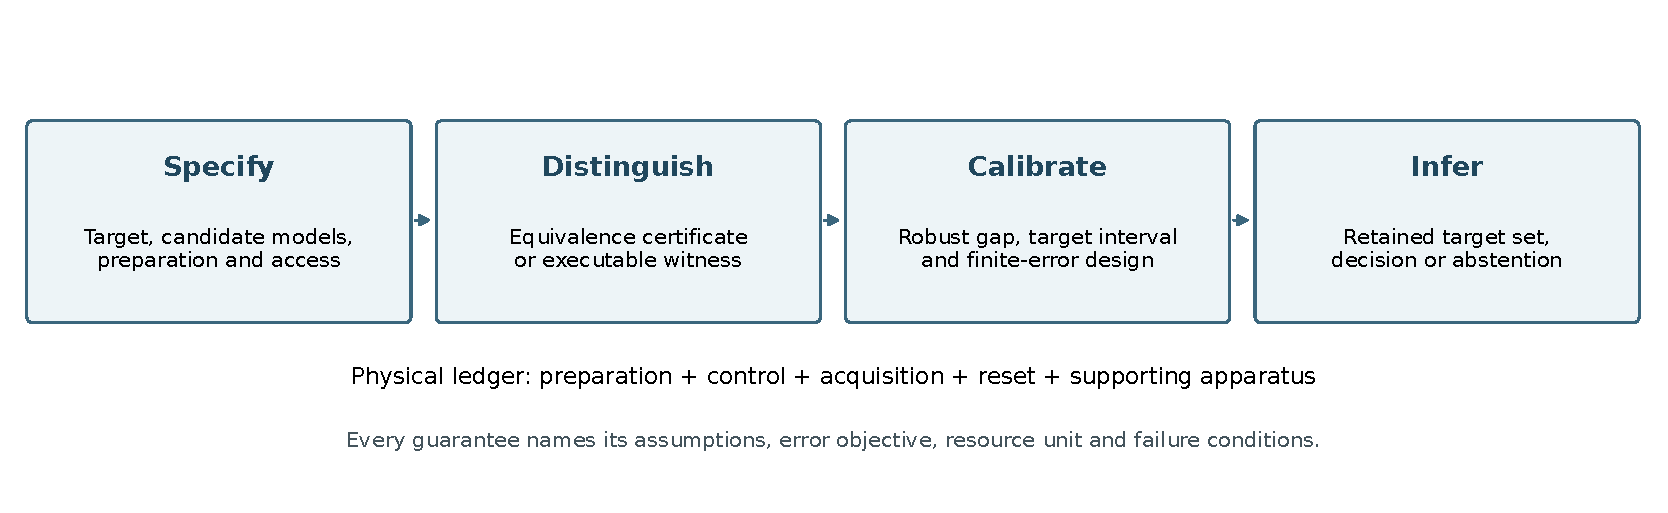
\includegraphics[width=\textwidth]{access_map.pdf}
\caption{The common workflow. Physical assumptions and resource accounting accompany the entire chain, rather than being inferred from a successful algebraic test.}
\label{entry:map}
\end{figure}

\section{A target beyond a supplied list of mechanisms}
The two-state example compares known alternatives. The physical results later
in the reference also bound entire model classes. One example asks how many
hidden classical states are needed to explain two preparation experiments.
Measure their contrast $C_0$ at a common reference time, then measure the same
contrast $C_T$ at a uniformly randomized later time. Under common homogeneous
Markov dynamics and a fixed binary detector, every classical model with at most
three states satisfies $|C_0-C_T|\leq1$, regardless of its unknown rates,
preparation distributions or detector noise. The proof and failure controls
appear in Proposition~\ref{rr:dimension-robust}.

A violation therefore supplies a lower bound on classical realization size.
It does not select a unique replacement model: four classical states can explain
some violating integrated records. This example illustrates the broader
purpose of constructive access. A useful observation can constrain what any
explanation must contain, even when reconstructing the mechanism is impossible.

The extension in Chapter~\ref{rf:entry} asks the same question about larger
classical explanations and physical resources. A finite-data hierarchy forces
at least five classical states in one worked design. A constructive approximation
theorem explains why finite reset records cannot uniformly exclude classical
models of unrestricted size and preparation cost. Stationary correlation
experiments can instead impose dissipation requirements without selecting a
hidden architecture. Together these results identify which added access or
resource premise supports the desired conclusion.

\section{Writing a contract before fitting data}
The following questions specify the experiment rather than merely its interpretation.
\begin{enumerate}
\item \textbf{Target.} What quantity or decision matters? A current's sign, its magnitude, a heat rate, and the full microscopic mechanism are different targets.
\item \textbf{Candidate family.} Which systems remain possible, including nuisance parameters, unknown preparations and detector effects? A nuisance parameter fixed for an entire experiment must stay fixed when calculating its joint record law.
\item \textbf{Preparation.} What can be reset, sampled or conditioned on? A stationary initial distribution is a substantive premise. Independent repetitions require a justified reset or sampling mechanism.
\item \textbf{Operations.} Which controls and measurements can actually be performed, in what order, with what feedback and stopping rules? Unavailable controls do not belong in the witness search.
\item \textbf{Record.} What is retained, including time stamps, failed detections, aborts, and control outcomes? Postselection needs its own success probability and resource accounting.
\item \textbf{Calibration.} Which complete instrument or record laws are bounded, with what joint confidence? Matching one output marginal does not calibrate hidden-state updates.
\item \textbf{Error objective.} Is the goal a worst-case interval, an equal-prior decision error, a posterior risk, or an anytime error guarantee? These objectives need different proofs.
\item \textbf{Resources.} Which contributions to time, gross work, net dissipation, calls or storage are included? State the budget and its units, together with excluded apparatus contributions.
\end{enumerate}
A useful contract also names a negative control and a condition that would cause the inference to be withheld. The software provides such outcomes directly.

\section{The mathematical structure}
The framework has one common object: the map from a hidden mechanism and a permitted protocol to a probability law of accessible records,
\[
 (\theta,\pi)\longmapsto P_\theta^\pi.
\]
The parameter $\theta$ need not be a scalar. It may represent an entire classical or quantum model. A protocol $\pi$ includes the permitted sequence of preparations, actions, observations and decisions. A target $g(\theta)$ states what the scientist wants to learn.

The questions then have a natural order. First, do two mechanisms generate identical accessible laws? Second, is the target constant across those indistinguishable mechanisms? Third, can a finite experiment reveal a relevant difference? Fourth, does the difference survive calibration and sampling? Finally, can the experiment be executed within the stated physical constraints?

The first two questions make sense for very general systems. Finite constructive algorithms require additional structure. The exact algebraic engine in this reference handles finite-dimensional linear representations, including finite classical instruments and finite quantum instruments. Continuous-time approximations, uncertainty sets, and fixed resource budgets add further assumptions. A general definition is not a universal finite algorithm.

\section{How the reference is organized}
The foundations chapter defines targets, accessible laws and equivalence. Finite access turns these definitions into certificates and witness searches. Precision and design link exact differences to robust intervals, statistical error and bounded policies. Model adequacy and physical expenditure explain how conclusions can be withheld and how resource guarantees can be composed. Continuous thermodynamics connects the abstract language to actual transition channels, current measurements and boundaries. The application chapter works through chemistry, quantum diagnostics, sensing and hidden power.

The workflow chapter adds a finite-family procedure that identifies a shared target even when several mechanisms remain indistinguishable. The toolkit chapter documents installation, contracts and independently checked outputs. The closing research map records where the results came from, their relation to established work, and the measurements needed for adoption.

A reader applying the framework can begin with this chapter, run the small example, then use the relevant physical chapter. A reader evaluating the theory should follow the proofs and the assumption tables before interpreting the numerical results. The packaged source and reproducibility driver make both paths checkable.

\section{Scope and scientific status}
The reference integrates proved finite-model results, established mathematical tools, new software interfaces, exact worked examples and internal adversarial checks. It contains no newly measured biological, materials or hardware dataset. It does not establish a physical law governing arbitrary matter, unrestricted total energy, universal quantum characterization, or autonomous improvement of arbitrary computation.

Its foundational contribution is a disciplined interface between questions that are often treated separately: access, identifiability, intervention, calibration, decisions and physical resources. The interface is useful precisely because a limitation or failure in one layer remains visible in the next. Acceptance as a scientific subject depends on independent use, criticism and successful experiments; those cannot be supplied by a manuscript alone.

\chapter{Scientific questions as access problems}
\label{foundations:chapter}

\section{Start with a quantity, a system, and an experiment}

A scientist rarely needs every microscopic parameter of a system. A useful
question is usually narrower: which direction does a current flow, how much
fuel does a process consume, does a particular error mechanism occur, or which
of several interventions changes a reaction pathway? The framework begins
with that quantity and asks whether the available experiments can determine
it. This order matters. A model can contain invisible parameters while the
quantity of interest remains identifiable.

Here is a small example that will recur in more detailed physical form.
Suppose two parallel channels contribute positive rates $a$ and $c$ to the
same observed transition. A detector identifies only the total rate
$k=a+c$. Replacing $(a,c)$ by $(a+h,c-h)$, while keeping both positive,
preserves every observation whose law depends only on $k$. The total rate
is identifiable; the individual rates are not. If a calibrated intervention
multiplies the first channel by a known $r\ne1$, a second observed total
$k_r=ra+c$ gives
\begin{equation}\label{foundations:twochannel}
 a=\frac{k-k_r}{1-r},\qquad c=\frac{k_r-rk}{1-r}.
\end{equation}
The intervention changes what can be identified. When $r$ is close to one,
the same formulas amplify measurement and calibration error. If $r$ is
unknown, the new observation need not remove the ambiguity. Thus an
experimental design requires both a model of intervention and a statement
of its accuracy.

The general object is an \emph{access specification}. It contains:
\begin{enumerate}
\item a candidate family $\Theta$, including nuisance parameters and the
      assumptions that make it a physically admissible family;
\item a target $g:\Theta\to\mathcal G$, with the units and required
      precision or decision loss stated;
\item available preparations, controls, measurements, retained records,
      and the rules governing their histories;
\item a calibration model and a resource account, including preparation,
      reset, sensing, control, and acquisition where these are used.
\end{enumerate}
This specification is a scientific input. Algebra can test its consequences;
it cannot establish from notation alone that an apparatus realizes it.
In particular, knowledge of the transition probabilities does not determine
the energy used by an unobserved subsystem.

Preparation belongs to access. A system that starts in an unknown state can
be observationally equivalent to a different system with another preparation.
A known reset, an independently calibrated stationary preparation, or a
recorded preparation outcome can change that conclusion. If preparation
depends on an unknown physical parameter, that dependence belongs in the
candidate model. It is not information available to the experimenter for
free.

\section{Transcript laws and targets}

Let $\mathcal A$ denote an access specification and $\Pi_{\mathcal A}$ its
permitted protocols. A protocol $\pi$ selects actions causally from retained
observations and any recorded or modeled randomization; it specifies when
to stop. Its complete accessible transcript has probability law
$P_\theta^\pi$ under candidate $\theta$. A transcript may contain action
choices, timestamps, detector outputs, preparation outcomes, and stopping
information. Omitting one of these changes the law being compared.
The same protocol is used under every candidate. A policy that secretly
knows the true candidate is not an experiment for distinguishing candidates.

\begin{definition}[Operational equivalence]\label{foundations:equivalence}
For a fixed access specification, write
\begin{equation}
 \theta\sim_{\mathcal A}\theta'
 \quad\Longleftrightarrow\quad
 P_\theta^\pi=P_{\theta'}^\pi
 \quad\text{for every }\pi\in\Pi_{\mathcal A}.
\end{equation}
The complete law profile is
$\Phi_{\mathcal A}(\theta)=(P_\theta^\pi)_{\pi\in\Pi_{\mathcal A}}$.
A target is \emph{structurally identifiable under $\mathcal A$} when
equality of these profiles implies equality of the target.
\end{definition}

This is identifiability from ideal experiment laws. It does not mean that
a finite noisy record determines a real parameter exactly. The distinction
is standard in statistical and dynamical-system identification
\cite{f_nemcova,f_thon}. It remains essential when the word ``observable''
is used with different conventions in different fields.

\begin{theorem}[Target factorization]\label{foundations:factorization}
A target $g$ is structurally identifiable under $\mathcal A$ if and only if
it is constant on each equivalence class of $\sim_{\mathcal A}$. Equivalently,
there is a unique map $\bar g$ on the attained profiles
$\Phi_{\mathcal A}(\Theta)$ such that
\begin{equation}
 g=\bar g\circ\Phi_{\mathcal A}.
\end{equation}
\end{theorem}
\begin{proof}
If a factorization exists, equal profiles have equal images under
$\bar g$ and hence equal targets. Conversely, define
$\bar g(\Phi_{\mathcal A}(\theta))=g(\theta)$. Constancy on each class
makes this definition independent of the representative. Every element
of the attained profile space has such a representative, proving uniqueness.
\end{proof}

The theorem is a set-theoretic quotient statement, not a claim that the
factor map is measurable, continuous, numerically stable, or efficiently
computable. Those properties need additional structure. Its practical use
is to separate an experimental obstruction from a difficult calculation.
An algorithm cannot reconstruct a target that takes two values on the
same attained profile without using further assumptions or further access.

For example, a hidden-state model may have several coordinate descriptions
related by a relabeling of latent states. Individual coordinates need not be
identifiable, while predictions and invariant target quantities are. The
quotient treats such representational ambiguity and physically different
but observationally equivalent mechanisms by the same mathematical rule.
Their scientific interpretations still differ.

\section{Processing, comparison, and the value of additional access}

For probability laws on a common measurable space define
\begin{equation}
 \operatorname{TV}(P,Q)=\sup_B|P(B)-Q(B)|.
\end{equation}
For a finite record alphabet this equals
$\frac12\sum_y|P(y)-Q(y)|$. A randomized processing rule is a Markov
kernel $K$: it maps a complete record to a reported statistic or decision
without knowing the true candidate.

\begin{proposition}[Data processing and access refinement]
\label{foundations:processing}
For any Markov kernel $K$,
\begin{equation}
 \operatorname{TV}(KP,KQ)\leq\operatorname{TV}(P,Q).
\end{equation}
Suppose every protocol $\pi$ available under $\mathcal A$ can be simulated
by some protocol $\rho$ under $\mathcal B$, followed by a
candidate-independent kernel $K$, so that
$P_\theta^\pi=K P_\theta^\rho$ for all $\theta$. Then
$\theta\sim_{\mathcal B}\theta'$ implies
$\theta\sim_{\mathcal A}\theta'$. Every target identifiable under
$\mathcal A$ is therefore identifiable under $\mathcal B$.
\end{proposition}
\begin{proof}
For any output event $B$, the function $z\mapsto K(z,B)$ takes values in
$[0,1]$. Integrating this function against $P-Q$ has absolute value at most
$\operatorname{TV}(P,Q)$, by the layer-cake representation as an integral
of indicator functions. Taking the supremum over $B$ proves contraction.
If the two $\mathcal B$ laws coincide, applying their common kernel gives
equal $\mathcal A$ laws for every $\pi$. Target identifiability then follows
from Theorem~\ref{foundations:factorization}.
\end{proof}

This is the familiar comparison-of-experiments principle
\cite{f_blackwell}, used here to compare experimental capabilities. A more
accurate detector, a new control, a retained controller record, or an allowed
reset can refine the equivalence classes. Conversely, discarding the action
history or averaging away a temporal correlation can merge classes.
The comparison needs a real simulation relation: two devices with
different resolution or resource requirements are not ordered merely
because one has more components.

For two fixed candidates and a declared resource budget $C$, let
\begin{equation}\label{foundations:frontier}
 D_{\mathcal A}(C;\theta_0,\theta_1)
 =\sup_{\pi\in\Pi_{\mathcal A}(C)}
   \operatorname{TV}(P_{\theta_0}^\pi,P_{\theta_1}^\pi).
\end{equation}
Here $\Pi_{\mathcal A}(C)$ must specify whether $C$ bounds elapsed time,
gross supplied energy, expected energy, operation count, or another
quantity. These constraints define different feasible sets. If a simulation
preserves the stated budget, Proposition~\ref{foundations:processing}
also orders the corresponding discrimination frontiers.

For known equally likely alternatives, the infimum average error over
protocols and tests is
\begin{equation}\label{foundations:bayes}
 \varepsilon^*(C)=\frac{1-D_{\mathcal A}(C;\theta_0,\theta_1)}{2}.
\end{equation}
Indeed, for a fixed protocol the likelihood comparison selects the larger
of the two probabilities or densities at each record, giving error
$(1-\operatorname{TV})/2$. Optimizing over protocols proves the expression.
Suprema and infima need not be attained. In particular, $D=1$ can describe
a limiting sequence of improving experiments without any single finite
experiment having zero error.

If two candidates with different targets are equivalent, every randomized
decision has the same distribution under both. A binary decision between
the two has average success at most $1/2$ under equal priors. For a real
target, every estimate $\widehat g$ satisfies
\begin{equation}\label{foundations:losslower}
 \max_{i=0,1}\mathbb E_{\theta_i}
       |\widehat g-g(\theta_i)|
 \geq \frac{|g(\theta_0)-g(\theta_1)|}{2}.
\end{equation}
The expectations use the same law for $\widehat g$; the triangle
inequality bounds the sum of the two risks below by the target separation.
Unlimited reprocessing of the same accessible evidence cannot remove this
obstruction. Additional physical access or a justified restriction of the
candidate family can.

\section{A common geometry for uncertainty and abstention}

Exact equality is only one source of ambiguity. Calibration bounds and
finite records also leave sets of compatible candidates. Let $z$ be reported
evidence and let a specified relation $\mathcal R\subseteq\Theta\times
\mathcal Z$ describe what that evidence permits. Define
\begin{equation}
 \Theta(z)=\{\theta:(\theta,z)\in\mathcal R\},\qquad
 G(z)=\{g(\theta):\theta\in\Theta(z)\}.
\end{equation}
For example, the relation may be exact equality of an observable profile,
a deterministic measurement enclosure, or a confidence construction with
a separately proved coverage guarantee. These interpretations should be
recorded, because they support different conclusions.

\begin{proposition}[Compatible-target radius]\label{foundations:radius}
Suppose $g$ is real valued, $\Theta(z)$ is nonempty, and estimates may take
any value in $\mathbb R$. If $G(z)$ is bounded, write
$a=\inf G(z)$ and $b=\sup G(z)$. Then
\begin{equation}
 \inf_{t\in\mathbb R}\sup_{\theta\in\Theta(z)}|t-g(\theta)|
 =\frac{b-a}{2},
\end{equation}
attained at $t=(a+b)/2$. If $G(z)$ is unbounded, every finite estimate has
infinite worst-case absolute error.
\end{proposition}
\begin{proof}
For bounded $G(z)$, the supremum loss is
$\max\{|t-a|,|t-b|\}$, whether or not the endpoints are attained. Its
minimum is the half-width, attained at the midpoint. If $G(z)$ is unbounded,
there are target values arbitrarily far from each fixed $t$.
\end{proof}

An empty compatible set is an inconsistency between evidence and the
declared model/calibration contract, rather than a uniquely identified
mechanism. A nonempty set on which $g$ is constant supports an exact target
within that contract even when several mechanisms survive. A wide target
set supports an interval or abstention. If $\Theta(Z)$ covers the true
candidate with probability at least $1-\delta$, the target set $G(Z)$
inherits that same coverage; the geometric proposition does not create the
coverage guarantee. For categorical targets or another loss function, the
appropriate decision problem replaces the real-valued midpoint.

This elementary geometry gives the common meaning of several later outputs:
an exact obstruction, a calibrated target interval, and a refusal to make an
unsupported decision. The linear intervention theorem specializes it to a
computable global worst-case radius. Sequential model checking supplies
coverage under adaptive actions and stopping. Neither step assumes that
surviving candidates are the whole of nature.

\section{When pairwise certificates give a finite scientific program}

\begin{theorem}[Finite target-separating suite]
\label{foundations:suite}
Let $\Theta=\{\theta_1,\ldots,\theta_K\}$ be a finite family. Suppose
the permitted elementary experiments have finite transcript alphabets and
any selected finite list can be executed on fresh preparations, independently
conditional on the same fixed candidate. Assume structural target
identifiability relative to these experiments. Then at most
$K(K-1)/2$ experiments suffice to form a suite whose joint law separates
every pair with different target values. If the individual models have
finite linear representations, witnesses can be synthesized with the finite
bound of Theorem~\ref{finite:span}.
\end{theorem}
\begin{proof}
For each unordered pair with distinct targets, identifiability supplies an
experiment with unequal laws. On a finite alphabet, some transcript event
has unequal probability. Choose one such experiment for each pair, dropping
duplicates. Fresh preparation gives a product joint law for the suite under
each fixed candidate. Its marginal for the chosen pair's experiment differs,
so the joint laws differ for that pair. There are at most $K(K-1)/2$ pairs.
The finite-representation assertion follows by applying
Theorem~\ref{finite:span} to each pair.
\end{proof}

The fresh-preparation assumption is consequential: concatenating probes on
one uncontrolled evolving specimen need not preserve their earlier
discriminating laws. The fixed-candidate qualification prevents a nuisance
parameter from being redrawn between trials merely to simplify a likelihood.
The theorem gives a finite separation program, not a finite-sample accuracy
claim or an efficient selection algorithm. Positive gaps can be small.
Section~\ref{workflow:suite} turns this existence result into a
calibration-aware experiment-cover workflow with explicit sample bounds.

\section{What is universal here}

The law-profile, comparison, and compatible-target constructions apply to
any well-defined family of experiments and targets. They are universal in
that mathematical sense. Finite-dimensional algorithms, Markovian dynamics,
quantum instruments, calibrated interventions, and energy envelopes impose
additional assumptions to make particular questions constructive.

The broad scientific contribution is an explicit chain from a question to
an admissible experiment and a checked conclusion. Its components connect
established statistical decision theory, system identification, control,
and physical modeling. This volume does not infer new conservation laws
from the shared formalism, and it does not equate an access limitation with
a general limit on computation. It provides a way to locate the unresolved
distinction, state the extra access that would remove it, and test whether
that access is practical.

The original boundary-and-arrow question is one instance: fix the allowed
local record, compare candidate dynamics with different time orientations,
and ask whether orientation is constant on the resulting equivalence
classes. A geometric boundary must be modeled as a physical restriction on
preparation, dynamics, coupling, or measurement. It cannot be silently
replaced by an unspecified loss of information. This operational entry point
preserves the physical question while allowing the same tools to address
reaction channels, sensor design, and quantum error hypotheses.

\chapter{Finite instruments and independently checkable access}
\label{finite:chapter}

\section{Representing an experiment without discarding its disturbance}

This chapter makes the abstract law profile constructive for finite
classical and quantum models. The algebraic representation is shared; the
conditions that make a representation physically valid differ. Throughout,
states are row vectors and effects are columns. A chronological product
$M_{s_1}M_{s_2}$ means that operation $s_1$ occurs first.

For candidate $h\in\{0,1\}$, a classical action $a$ has a finite recorded
outcome set $\mathcal Y_a$ and matrices $K_h^{a,y}$ on $n_h$ hidden states.
The entry $K_h^{a,y}(x,x')$ is the joint probability of recording $y$ and
ending at $x'$ conditional on starting at $x$. Physical validity requires
\begin{equation}\label{finite:classical}
 K_h^{a,y}\geq0\quad\hbox{entrywise},\qquad
 \sum_{y\in\mathcal Y_a}K_h^{a,y}\mathbf1=\mathbf1.
\end{equation}
The initial distribution $x_h$ is nonnegative and satisfies $x_h\mathbf1=1$.
An abort or failed preparation is a possible recorded outcome when it can
occur. Deleting its probability and renormalizing would define a different
experiment, usually with an unaccounted selection and preparation cost.

For a word of action/outcome pairs
$w=((a_1,y_1),\ldots,(a_m,y_m))$, the joint event probability is
\begin{equation}\label{finite:probability}
 p_h(w)=x_hK_h^{a_1,y_1}\cdots K_h^{a_m,y_m}\mathbf1.
\end{equation}
This expression retains both measurement probabilities and the change of
hidden state caused by measurement. An outcome-only noise model generally
cannot replace it when the detector disturbs subsequent dynamics.

For a quantum system of Hilbert dimension $q_h$, an action instead consists
of completely positive trace-nonincreasing maps
$\mathcal E_h^{a,y}$ whose sum is trace preserving. From density operator
$\rho_h$, the probability is
\begin{equation}
 p_h(w)=\operatorname{tr}\!\left[
 \mathcal E_h^{a_m,y_m}\circ\cdots\circ
 \mathcal E_h^{a_1,y_1}(\rho_h)\right].
\end{equation}
Expressing Hermitian operators in a real basis gives a row-state linear
representation with dimension $n_h=q_h^2$ and a terminal column $\tau_h$
representing trace. Transfer matrices can have negative entries in that
basis. Entrywise stochastic positivity is not a quantum validity test;
complete positivity and trace preservation must be established from the
instrument, for example through its Kraus operators.

Both cases therefore have the form
\begin{equation}\label{finite:linear}
 p_h(w)=x_hM_h^w\tau_h,\qquad
 M_h^w=M_h^{a_1,y_1}\cdots M_h^{a_m,y_m},
\end{equation}
on the common finite alphabet
$\Sigma=\{(a,y):y\in\mathcal Y_a\}$. A generic signed linear
representation is an algebraic input; it does not automatically define
probabilities. The exact software uses rational entries and recomputes
identities with rational arithmetic. The finite-dimensional theorems also
hold over the reals, but floating-point near-equality is not an exact
equivalence certificate.

\section{Finite closure decides equality of every finite record}

Pair two representations by setting
\begin{equation}\label{finite:paired}
 \alpha=(x_0,-x_1),\qquad
 \beta=\begin{pmatrix}\tau_0\\\tau_1\end{pmatrix},\qquad
 M_s=\begin{pmatrix}M_0^s&0\\0&M_1^s\end{pmatrix},\qquad
 d=n_0+n_1.
\end{equation}
Their contrast is $f(w)=\alpha M_w\beta=p_0(w)-p_1(w)$.
Let
\begin{equation}\label{finite:space}
 V=\operatorname{span}\{M_w\beta:w\in\Sigma^*\}.
\end{equation}
The generating columns are actual event effects; arbitrary linear
combinations in $V$ need not be effects of implementable measurements.
The span is a computational device for proving statements about the
generating experiments.

\begin{theorem}[Finite effect-space criterion]\label{finite:span}
For a finite alphabet and finite-dimensional representation, all contrasts
vanish if and only if $\alpha V=0$. If $\beta\ne0$ and some contrast is
nonzero, there is a distinguishing word of length at most $d-1$.
For valid instrument models this is equivalent to equality of the complete
laws of every fixed finite action sequence. Such equality also implies
equality under every common causal classical policy with almost surely
finite stopping under both models.
\end{theorem}
\begin{proof}
Let $V_k$ span effects of length at most $k$. Then
\begin{equation}
 V_0=\operatorname{span}\{\beta\},\qquad
 V_{k+1}=V_k+\sum_{s\in\Sigma}M_sV_k.
\end{equation}
If $V_{k+1}=V_k$, the space is invariant under all letters and contains
every word effect. Otherwise its dimension strictly increases. Starting
from dimension one, at most $d-1$ increases are possible. Hence
$V_{d-1}=V$, proving both the criterion and the witness bound. The case
$\beta=0$ has zero contrast for every word.

For valid instruments, words with a prescribed action sequence are the
atoms of its complete outcome law, so equality of all their probabilities
is precisely equality of that law. Under a causal randomized policy, a
complete action/outcome history has its instrument word probability
multiplied by the common probabilities with which the policy chooses its
actions and stopping along that history. These factors are identical under
both candidates. Equality therefore holds at each finite terminal history;
summing over the countable terminal histories proves equality for almost
surely finite stopping. Conversely, fixed action sequences are policies.
\end{proof}

Finite-span equivalence and short counterexample words are established
results for weighted and probabilistic automata
\cite{f_tzeng,f_kiefer,f_notes}. Observable operator models and predictive
state representations supply closely related descriptions of controlled
hidden dynamics \cite{f_thon,f_jaeger,f_littman}. Quantum equivalence also
has established finite-dimensional formulations \cite{f_wang}. The
framework uses these results as its exact algebraic foundation.

The allowed memory and control architecture must be represented. Arbitrary
unmodeled ancillas, coherent feedback, or additional continuous control
values are not included by calling the protocol ``adaptive.'' A specified
finite quantum memory can be included in the state dimension. Enlarging
that architecture changes the access problem.

\subsection{A certificate another implementation can check}

An equivalence certificate supplies columns $b_1,\ldots,b_r$, together with
coefficients establishing
\begin{equation}\label{finite:closure}
 \beta\in\operatorname{span}\{b_i\},\qquad
 M_s b_i\in\operatorname{span}\{b_j\}\quad\text{for all }s,i,
 \qquad \alpha b_i=0.
\end{equation}
Induction on word length places every $M_w\beta$ in the supplied span,
so every contrast vanishes. Linear independence of the columns is useful
for compact generation but unnecessary for sound checking. A non-equivalence
certificate supplies an actual word and its nonzero exact contrast. Neither
certificate requires the reviewer to trust the search execution.

For a minimal entry example, a one-state instrument emits a bit with
probability $p_h$ under action $a$. Its scalar kernels are $M_h^{a,1}=p_h$
and $M_h^{a,0}=1-p_h$. With $p_0=1/2$, $p_1=3/5$, the word $(a,1)$
has contrast $-1/10$, and the bound $d-1=1$ is attained. Both outcomes
remain possible under both hypotheses, so this exact witness is not a
perfect discriminator. Repeated sampling belongs to the statistical layer.

\section{Constraints on experiment histories}

Apparatus rules can prohibit particular action orders or require a
preparation and final readout. For an action-only deterministic finite
automaton, let $q_0$ be its initial state, $F$ its accepting states, and
$\delta(q,a)$ its possibly undefined transition. The matrix $A_a$ has entry
one at $(q,\delta(q,a))$ when that transition is defined and zero otherwise.
Let $v_F$ indicate accepting states. With $S$ automaton states, replace
\begin{equation}\label{finite:grammar}
 x_h\mapsto e_{q_0}^{\mathsf T}\otimes x_h,\qquad
 M_h^{a,y}\mapsto A_a\otimes M_h^{a,y},\qquad
 \tau_h\mapsto v_F\otimes\tau_h.
\end{equation}
The resulting series is the physical word probability on accepted complete
action sequences and zero elsewhere. It is a masked algebraic series,
not itself a normalized physical instrument on all strings. Applying
Theorem~\ref{finite:span} in paired dimension $Sd$ proves equality on
accepted experiments or produces an accepted witness of length at most
$Sd-1$. The lift is a standard finite-language construction, consistent
with constrained switching realization theory
\cite{f_petreczky,f_bastug}.

Nonaccepting intermediate grammar states are allowed. A protocol can pass
through one while continuing toward a legal completed experiment. Stopping
there is inadmissible. An empty accepted language gives a vacuous equality
certificate. For adaptive policies the supported terminal action sequences
must satisfy the grammar almost surely under both candidates.

Outcome-dependent restrictions require further care. A language that
retains only selected successful outcomes can describe postselection rather
than executable access. A physical specification must say what happens on
the excluded outcomes and how their probability and cost are retained.
The implemented grammar here is action-only; it does not silently solve
that more general policy-feasibility problem.

\section{The cheapest nonzero witness}

Give every action a nonnegative rational charge $c(a)$, independent of its
outcome and prior history, and define the lexicographic weight
\begin{equation}\label{finite:weight}
 \omega(w)=\left(c(w),|w|\right),\qquad
 c(w)=\sum_{j=1}^{|w|}c(a_j).
\end{equation}
The length component selects the shortest among equal-charge witnesses.
An action charge may be a calibrated upper bound on gross energy, a
specified duration, or a count. The theorem optimizes the supplied
additive quantity. A mean physical cost depending on the hidden state or
realized path generally does not have this form.

Use a priority queue ordered by $\omega$, with a deterministic final tie
breaker. Initially it contains $(\beta,\varnothing)$. Remove the least
candidate $(v,w)$. If $v$ is in the span of previously retained columns,
discard it. Otherwise retain the column and its actual word. Return $w$
if $\alpha v\ne0$. If the contrast is zero, insert every
$(M_s v,sw)$, where $sw$ prepends the letter $s$ to the chronological
word. This backward construction of effects does not reverse the
chronology of the resulting physical protocol.

\begin{theorem}[Cost-priority closure]\label{finite:cost}
The search accepts at most $d$ columns and removes at most
$1+|\Sigma|d$ candidates. It returns either an equivalence certificate or
a minimum-charge nonzero word, shortest among all minimum-charge nonzero
words. Zero-charge actions are allowed. The same result applies after
the grammar lift with its enlarged dimension.
\end{theorem}
\begin{proof}
Each retained column increases rank and only retained zero-contrast columns
generate candidates. This gives both finite bounds. In particular, the
search cannot loop through infinitely many zero-charge words.

A discarded candidate is a linear combination of earlier retained
columns. Since prepending increases length by one and adds a nonnegative
charge, queue removal weights never decrease. Every column in that
combination has weight no larger than the discarded candidate. Prepending
the same letter to the combination preserves the identity and the weight
ordering.

For completeness of this pruning rule, fix a weight threshold $T$ and
consider the state after all generated candidates of weight below $T$
have been processed, assuming none has nonzero contrast. Induct on word
length. The empty effect has been retained or expressed in retained
columns whenever its weight is below $T$. For $w=sv$ below $T$, the
inductive representation of $M_v\beta$ uses columns of weight at most
$\omega(v)$. Each of their $s$ prefixes was generated and has weight at
most $\omega(w)<T$. On processing, it was either retained or replaced by
earlier columns of no greater weight. Thus every below-threshold word
effect lies in the retained span, with no greater representative weight.

Before the returned witness, all retained effects have zero contrast. A
cheaper, or equal-charge shorter, nonzero word would have an effect in
their span, a contradiction. If the queue empties, the retained span
contains $\beta$ and every prefixed retained effect, and is annihilated
by $\alpha$. Equation~\eqref{finite:closure} then certifies equivalence.
\end{proof}

The returned word also gives a minimum-charge fixed action sequence whose
complete outcome laws differ: every outcome word for the same sequence has
the same action charge. It is an event to count while executing that action
sequence and retaining all outcomes. The witness does not confer a right
to postselect its outcomes without accounting for the failures.

This specialization is built on established finite-rank search. Its
historical priority is not established by this volume. It is useful because
it aligns a qualitative witness with a declared physical protocol charge.
It does not minimize repetitions, finite-error risk, total energy, or the
expected cost of adaptive stopping. A cheaper tiny gap can require much
greater total acquisition than a more expensive strong measurement.

\section{Certifying optimality without trusting the optimizer}

A reviewer should be able to verify more than the fact that a supplied
word distinguishes the candidates. The following certificate also proves
the declared minimum charge. Let $w_*$ be the proposed witness and
$T=\omega(w_*)$. Supply a finite list of actual-word effects
\begin{equation}
 b_i=M_{u_i}\beta,\qquad t_i=\omega(u_i)<T,
 \qquad\alpha b_i=0,
\end{equation}
and exact expansion coefficients with the following conditions:
\begin{align}
 \beta&=\sum_i r_i b_i,
 &r_i\ne0&\ \Longrightarrow\ t_i\leq(0,0),
 \label{finite:filteredbeta}\\
 M_s b_i&=\sum_j q_{sij}b_j,
 &q_{sij}\ne0&\ \Longrightarrow\
 t_j\leq t_i+(c(s),1).
 \label{finite:filteredclosure}
\end{align}
Require the initial expansion when $(0,0)<T$. Require the prefix expansion
for every $(s,i)$ with $t_i+(c(s),1)<T$. Recompute each effect, weight, and
contrast from the declared model and word. In particular, verify
$\alpha M_{w_*}\beta\ne0$.

\begin{theorem}[Filtered optimality certificate]
\label{finite:filtered}
A proposed nonzero word is minimum-charge and shortest among
minimum-charge nonzero words if and only if a finite certificate satisfying
these conditions exists. The certificate is sound with redundant columns,
signed matrices, and zero-charge actions.
\end{theorem}
\begin{proof}
For soundness, consider $w$ with $\omega(w)<T$. Induct on its length to
express $M_w\beta$ using only $b_i$ with $t_i\leq\omega(w)$. The empty
word uses Eq.~\eqref{finite:filteredbeta}. For $w=sv$, nonnegative
charges and the length tie-break give
$\omega(v)<\omega(sv)<T$. Every effect used for $v$ satisfies
\begin{equation}
 t_i+(c(s),1)\leq\omega(sv)<T.
\end{equation}
The corresponding required identity
\eqref{finite:filteredclosure} propagates the representation and its
weight bound. Since $\alpha b_i=0$, all below-threshold contrasts vanish.
The supplied nonzero witness therefore has the claimed optimum. When
$T=(0,0)$ there are no smaller words and no initial expansion is needed.

For completeness, run the cost-priority construction through all generated
candidates below $T$. If $w_*$ is optimal, every retained effect there
has zero contrast. Each processed discarded effect has an expansion in
earlier columns of no greater weight. The initial effect and every required
prefix were processed, giving the displayed identities. At most $d$
independent columns are needed, so this construction terminates even when
some actions have zero charge.
\end{proof}

For full equivalence, omit the threshold, require an expansion of $\beta$
and every prefix, and require zero contrast on all supplied columns.
This is both sound and complete by finite closure. The checker needs only
matrix multiplication, rational arithmetic, and the explicit expansion
identities; it need not calculate a basis or call an optimizer.

The weight restriction in the expansion is essential. Replacing a cheap
effect by an expensive representative without tracking its weight can
remove a required cheap prefix from the certificate and hide a cheaper
witness. Exact closure alone proves equivalence when imposed globally;
partial closure proves an optimum only when its filtration is respected.
The software tests deliberately forged word costs, missing prefixes,
model substitutions, and genuine but nonminimal witnesses.

A certificate must be bound to the model the reviewer intends to check.
A digest of an embedded model establishes internal consistency, but an
adversary could replace both model and digest. The checker therefore accepts
an independently selected expected model or digest. A digest is neither a
signature nor a calibration measurement. Physical validity and empirical
model adequacy remain separate requirements.

\section{What finite dimension does and does not make easy}

The dimension bound concerns the supplied representation. For two generic
$n$-qubit instruments, each real operator space has dimension $4^n$ and
the paired dimension is $2\cdot4^n$. Finite linear algebra therefore does
not imply a polynomial algorithm in qubit count, constant-shot process
characterization, or elimination of fault-tolerance overhead. Known
structure and a narrow target can reduce the represented problem, but
those are additional assumptions.

The number of rank operations is finite and polynomial in the explicit
matrix dimension for standard implementations. Exact arithmetic also incurs
bit complexity, and certificate size includes its rational coefficients.
A short word need not have a large probability contrast. Consequently a
bound on witness length is not a bound on the records required for reliable
inference. The statistical chapter keeps these quantities distinct.

\subsection{Parameterized families and an algebraic route}

Suppose every model has fixed representation dimension $n$, matrix entries
are rational functions of parameters $\theta$ on a semialgebraic domain,
and all denominators are nonzero there. Suppose the domain and functions
are effectively given over the rationals or algebraic numbers. For a
parameter pair $(\theta,\theta')$, Theorem~\ref{finite:span} makes
equivalence a finite collection of word-probability equalities for lengths
at most $2n-1$. Clearing nonvanishing denominators gives polynomial
conditions. For a rational target $g$, structural identifiability is the
validity of
\begin{equation}
 \forall\theta,\theta'\in\Theta:\quad
 \left(\bigwedge_{|w|\leq2n-1}p_\theta(w)=p_{\theta'}(w)\right)
 \Longrightarrow g(\theta)=g(\theta').
\end{equation}
Real quantifier elimination decides this statement in principle
\cite{f_basu,f_nemcova}. The finite conjunction can be enormous and the
decision can be computationally expensive. The observation is a route for
appropriately structured symbolic problems, not an implemented solver for
arbitrary continuous families. It also explains where algebraic geometry
enters naturally: the fibers of the observable map are polynomial or
rational constraint sets in such a model.

\section{An exact boundary for unbounded positive-gap search}

Deciding whether any word has a nonzero contrast is easier than deciding
whether some arbitrarily long experiment exceeds a fixed positive
discrimination threshold.

\begin{theorem}[Strict-cutpoint boundary in instrument form]
\label{finite:undecidable}
Fix a rational $\delta\in(0,1)$. There is no algorithm that, for every
pair of finite rational classical instruments with the following grammar,
decides whether some admissible finite protocol has transcript total
variation greater than $\delta$: any finite sequence of unobserved
stochastic actions, followed by exactly one terminal binary readout.
The horizon is unbounded and no repeated independent preparation is
available within a protocol.
\end{theorem}
\begin{proof}
Use the established undecidability of strict cutpoint emptiness for
rational probabilistic finite automata, in particular the fixed cutpoint
$1/7$ result described and proved in Ref.~\cite{f_rote}. Such an automaton
has initial distribution $\mu$, stochastic letter matrices $T_a$, and
binary acceptance column $v$. Its acceptance probability for word $w$ is
$p(w)=\mu T_wv$. The undecidable question is whether $p(w)>1/7$ for some
finite word.

Turn each letter into a single-outcome unobserved action. After these
actions allow one terminal readout with success effect
$D=aI+b\operatorname{diag}(v)$ and failure effect $I-D$. Choose rational
$b>0$ small enough that $a=\delta-b/7\geq0$ and $a+b\leq1$. These
diagonal readout kernels are physically valid classical instruments.
Compare against a one-state model that always reports zero. The only
informative observation is Bernoulli success with probability
$a+bp(w)$ versus certain failure; its total variation is $a+bp(w)$.
It exceeds $\delta$ exactly when $p(w)>1/7$.

All outcomes preceding the readout are deterministic, so feedback supplies
no information for choosing the word. If the chosen word is recorded,
randomization gives the average of its total variations, since the word
distribution is common to both models. If that average exceeds the
threshold, some deterministic word exceeds it. Thus an algorithm for
the stated instrument problem would decide strict cutpoint emptiness.
\end{proof}

This is a translation of an established computability result, historically
traced to Nasu and Honda, rather than a new impossibility theorem for
physics. The reduction does not show that its stochastic matrices are
embeddable continuous-time propagators, thermodynamically reversible, or
available in any particular laboratory. Allowing unlimited independent
resets and repeated measurements changes the problem: a nonzero single-run
gap can then be amplified statistically.

A finite horizon makes the specified finite-alphabet design problem
finite. A finite additive budget does so only when every repeatable action
has a strictly positive minimum charge, or a separate horizon is imposed.
Zero declared entropy production does not imply zero laboratory energy,
and a budget on one accounting channel need not bound the number of
possible operations. Bounded design, calibrated statistics, and physical
accounting are therefore required layers of the constructive framework.

\chapter{Precision, calibration, and experimental design}
\label{precision:chapter}

Exact identifiability asks whether some accessible record law changes when the
scientific target changes. Precision asks how much evidence is needed to resolve
that change. These questions have different answers. A nonzero rational contrast
can be arbitrarily small, an invertible response matrix can be arbitrarily poorly
conditioned, and a short distinguishing experiment can require many repetitions.
This chapter supplies upper and lower guarantees that connect the exact access
layer to decisions a scientist can use.

Throughout, $\theta$ denotes a fixed physical model, $g(\theta)$ the target, and
$P_\theta^\pi$ the law of the complete accessible record under a common permitted
protocol $\pi$. A resource contract specifies preparation, actions, stopping,
and the meaning of every budget. The general statistical ingredients below are
established: binary testing, optimal recovery, concentration, and belief-state
dynamic programming. Their role here is to make the interfaces explicit.

\section{What the best possible precision means}

For probability laws $P,Q$ on a common record space, use the convention
\[
 \operatorname{TV}(P,Q)=\sup_A|P(A)-Q(A)|
 =\tfrac12\int|p-q|\,d\mu,
\]
where $\mu$ dominates both laws. If the two models are known and equally likely,
the smallest average probability of choosing the wrong model is
\begin{equation}
 r^*(P,Q)=\frac{1-\operatorname{TV}(P,Q)}2.
 \label{precision:tv-risk}
\end{equation}
Indeed, choose the first model on $\{p\geq q\}$; the resulting error is
$\frac12\int\min(p,q)\,d\mu$, and pointwise minimization shows that no other
decision rule has smaller error. This is an average error for specified priors.
It is not automatically a bound on each of the two conditional errors.

Let $\Pi_C$ be the declared class of protocols admissible at resource budget $C$.
With the access setting fixed, abbreviate the frontier of
Equation~\eqref{foundations:frontier} by
\begin{equation}
 D_C(\theta_0,\theta_1)=
 \sup_{\pi\in\Pi_C}\operatorname{TV}(P_{\theta_0}^\pi,P_{\theta_1}^\pi).
 \label{precision:resource-discrimination}
\end{equation}
For known equal-prior alternatives, the infimum achievable average error is
$(1-D_C)/2$. A supremum need not be attained by a protocol. If the budget classes
are nested, $D_C$ is nondecreasing. No shape, universal energy scale, or efficient
algorithm for this function follows from its definition.

\begin{proposition}[A resource-dependent lower bound for real targets]
\label{precision:two-point}
Let $g$ be real valued, and let an estimator $T$ use the record of any
$\pi\in\Pi_C$. The policy, its randomization rule, and the estimator must be the
same under both alternatives. Then
\begin{equation}
 \max_{j=0,1}\mathbb E_{\theta_j}^{\pi}|T-g(\theta_j)|
 \geq \frac{|g(\theta_0)-g(\theta_1)|}{2}
 \bigl[1-\operatorname{TV}(P_{\theta_0}^\pi,P_{\theta_1}^\pi)\bigr].
 \label{precision:two-point-fixed}
\end{equation}
Consequently, for any parameter family $\Theta$,
\begin{equation}
 \inf_{\pi\in\Pi_C,\,T}\sup_{\theta\in\Theta}
 \mathbb E_\theta^\pi|T-g(\theta)|
 \geq \sup_{\theta_0,\theta_1\in\Theta}
 \frac{|g(\theta_0)-g(\theta_1)|}{2}
 [1-D_C(\theta_0,\theta_1)].
 \label{precision:two-point-resource}
\end{equation}
Expectations may be infinite. The bound is not asserted to be attainable.
\end{proposition}
\begin{proof}
Write $g_j=g(\theta_j)$ and $p_j=dP_{\theta_j}^\pi/d\mu$. The triangle inequality
gives, pointwise,
\[
 p_0|T-g_0|+p_1|T-g_1|
 \geq\min(p_0,p_1)(|T-g_0|+|T-g_1|)
 \geq |g_0-g_1|\min(p_0,p_1).
\]
Integration and $\int\min(p_0,p_1)=1-\operatorname{TV}(P_0,P_1)$ prove
\eqref{precision:two-point-fixed}. Independent estimator randomization is a
common probability kernel and the same argument applies after adjoining its
random seed. For every fixed pair, replacing the policy's total variation by
its supremum over $\Pi_C$ weakens the bound uniformly in $\pi$. Taking the
infimum on the left and then the supremum over pairs proves
\eqref{precision:two-point-resource}; no minimax interchange is used.
\end{proof}

This is the standard two-point method associated with Le Cam
\cite{caLeCamYang2000}. It identifies an important failure case: an invisible
target difference has $D_C=0$ at every allowed budget, so more computation on
the same records cannot remove its ambiguity. If invisible pairs have arbitrarily
large finite target separation, the worst absolute-error risk is infinite.
The conclusion follows by taking those finite pairs, without undefined products
involving infinity. A lower bound caused by restricted access is different from
a claim that all information about the system has a universal cap.

\section{Linear intervention responses: from rank to stable recovery}

Suppose $\theta\in\Theta\subset\mathbb R^p$ and a known matrix
$F\in\mathbb R^{m\times p}$ represents intervention responses. Two physical
assumptions are needed before its algebra describes the apparatus:
\begin{enumerate}
 \item If $F\theta=F\theta'$, every permitted complete record law agrees.
 \item If every permitted complete record law agrees, then $F\theta=F\theta'$.
\end{enumerate}
The first is law factorization; the second is access sufficiency. A hidden
generator's dependence on $F\theta$ may establish the first while leaving the
second unproved for a coarse detector. Unknown preparation or a
parameter-dependent detector can invalidate either identification argument.

For example, controlled continuous-time generators with known entries
$q_0+F\theta$ give factorization when preparations and readout are known and
parameter independent. Access sufficiency follows in an idealized setting where
every state is preparable and resolved, and transition laws are accessible at
arbitrarily short times: the derivative at zero identifies each generator entry.
Finite bandwidth and finite data require additional bounds; that idealization
does not provide them.

\begin{proposition}[A target-specific row-space criterion]
\label{precision:row-space}
Assume both conditions above and a nonempty open domain $\Theta$. The linear
target $g(\theta)=b^{\mathsf T}\theta$ is identifiable if and only if
$b\in\operatorname{row}(F)$, equivalently $F^{\mathsf T}w=b$ for some $w$.
\end{proposition}
\begin{proof}
Such a $w$ yields $g(\theta)=w^{\mathsf T}F\theta$, so access sufficiency proves
the claim. Conversely, if $b$ is outside the row space, there is
$h\in\ker(F)$ with $b^{\mathsf T}h\ne0$. At an interior point $\theta_*$,
both $\theta_*+th$ and $\theta_*-th$ are allowed for sufficiently small $t>0$.
Factorization makes their laws identical, while their targets differ.
\end{proof}

On a relatively open affine parameter domain $\theta_*+V$, the correct condition
is that $b$ annihilate $V\cap\ker F$. Known constraints can therefore resolve
ambiguities that remain on the full open domain. Full parameter reconstruction
requires more than reconstruction of a particular scientific target.

Now suppose the measured or statistically estimated response satisfies
\begin{equation}
 \widehat y=F\theta+e,\qquad |e_i|\leq\epsilon_i,
 \label{precision:response-error}
\end{equation}
where every $\epsilon_i$ is known and nonnegative. Any $F^{\mathsf T}w=b$ gives
\begin{equation}
 |w^{\mathsf T}\widehat y-b^{\mathsf T}\theta|
 \leq \sum_i\epsilon_i|w_i|.
 \label{precision:linear-upper}
\end{equation}
No independence of coordinate errors is needed. If the entire box is certified
with probability at least $1-\delta$, this deterministic conclusion has at least
that coverage. How the box is obtained remains a separate experimental question.

\begin{theorem}[Global deterministic minimax recovery]
\label{precision:linear-minimax}
Assume the parameter domain is the entire positive orthant
$\mathbb R^p_{>0}$, $F$ is known, and every error vector in the full Cartesian
box $[-\epsilon,\epsilon]$ is admissible. If $b\in\operatorname{row}(F)$, then
\begin{align}
 &\inf_T\sup_{\theta>0,\,|e|\leq\epsilon}
       |T(F\theta+e)-b^{\mathsf T}\theta| \nonumber\\
 &\hspace{8mm}=\min_{F^{\mathsf T}w=b}\sum_i\epsilon_i|w_i|
   =\max_{|Fh|\leq\epsilon}b^{\mathsf T}h.
 \label{precision:linear-duality}
\end{align}
The extrema on the right exist, including when some error radii vanish.
If $b\notin\operatorname{row}(F)$, the recovery risk is infinite, the middle
problem is infeasible, and the dual supremum is unbounded.
\end{theorem}
\begin{proof}
Equation~\eqref{precision:linear-upper} proves the upper bound. For any dual-feasible
$h$, choose a componentwise center $\theta_*>|h|$. The two positive parameters
$\theta_*\pm h$, with errors $\mp Fh$, produce the same observation
$\widehat y=F\theta_*$. Their target separation is $2|b^{\mathsf T}h|$.
Every estimate at that common observation errs by at least $|b^{\mathsf T}h|$
on one of them. The feasible set for $h$ is symmetric, giving the displayed
dual lower bound.

Write $w=u-v$, $u,v\geq0$. The middle value equals the linear program
\[
 \min_{u,v\geq0}\epsilon^{\mathsf T}(u+v)
 \quad\hbox{subject to }F^{\mathsf T}u-F^{\mathsf T}v=b.
\]
Its dual is exactly $\max b^{\mathsf T}h$ subject to
$Fh\leq\epsilon$ and $-Fh\leq\epsilon$. The primal is feasible with a finite
nonnegative infimum, and the dual is feasible at zero. Finite-dimensional linear
programming duality supplies attainment and equality \cite{caBoyd2004}.
If $b$ is outside the row space, scale an $h\in\ker F$ with
$b^{\mathsf T}h>0$ and repeat the common-observation construction to obtain
arbitrarily large error lower bounds.
\end{proof}

An independently checkable certificate consists of $w,h$ satisfying
$F^{\mathsf T}w=b$, $|Fh|\leq\epsilon$, and
$\sum_i\epsilon_i|w_i|=b^{\mathsf T}h$. The checker need not trust the optimizer.
This is a structured, globally worst-case specialization of the compatible-set
geometry in Proposition~\ref{foundations:radius}. A particular observed
$\widehat y$ may give a smaller feasible target interval. Bounded parameter
domains or correlated error constraints can also lower the minimax value;
their replacement by the full positive orthant or full error box changes the
problem being solved.

\subsection{A calibrated intervention example}

Two unresolved positive channel rates have baseline response
$y_0=\theta_1+\theta_2$. A calibrated intervention produces
$y_1=r\theta_1+\theta_2$, with known $r\geq0$. Thus
\[
 F_r=\begin{pmatrix}1&1\\r&1\end{pmatrix},\qquad
 \theta_1=\frac{y_1-y_0}{r-1}\quad(r\ne1).
\]
At equal response-error radius $\epsilon$, the exact global minimax error for
$\theta_1$ is $2\epsilon/|r-1|$. For the primal choose
$w=(-1,1)/(r-1)$; a matching dual is
$h=\epsilon(2,-r-1)/|r-1|$. Its two response coordinates have magnitudes
$\epsilon$, and its first component equals the claimed error.
At $\epsilon=0.01$, responses $r=1/2,0.9,0.99,0.999$ give errors
$0.04,0.2,2,20$. At $r=1$ the channel is unidentifiable. Exact full rank near
$r=1$ does not establish useful precision.

Adding a third response with $r=2$ to the baseline and $r=1/2$ gives, at the
same three error radii $0.01$, optimal weights $(0,-2/3,2/3)$ and error $1/75$.
The dual $h=(1/75,-1/60)$ proves optimality. This improvement presumes that
the extra measurement does not worsen the existing error bounds; a fixed
physical budget may require a different comparison.

Unknown selectivity is a decisive control: $(\theta_1,\theta_2,r)=(3,1,1/2)$
and $(2,2,1/4)$ both give $(y_0,y_1)=(4,5/2)$. Inserting a nominal $r$ into a
known-matrix certificate does not validate it when $r$ is unknown.

\section{From one record to a finite-error experiment}

\subsection{Known laws and affinity}

For known finite record laws define their Bhattacharyya affinity
\cite{caBhattacharyya1943}
\[
 \rho(P_0,P_1)=\sum_z\sqrt{P_0(z)P_1(z)}.
\]
Cauchy--Schwarz gives $0\leq\rho\leq1$, with equality at one exactly when the
two laws agree. For $M$ independent records under the same fixed model,
the likelihood-ratio decision rule has equal-prior average error at most
\begin{equation}
 r_M^*\leq\tfrac12\rho(P_0,P_1)^M.
 \label{precision:affinity}
\end{equation}
To prove this, use $\min(p,q)\leq\sqrt{pq}$ in
Equation~\eqref{precision:tv-risk}; affinity multiplies over product laws.
An outward rational upper bound $\overline\rho<1$ therefore certifies a
sufficient record count. An upper enclosure at least one certifies no such
count at that precision. It need not mean that the actual laws are equal.

The product-law premise requires independent preparations or a justified
independent-record construction. If a nuisance parameter is fixed but unknown,
it stays fixed in every factor. Averaging its law independently at every record
models a different experiment. Full common support also prevents perfect
finite-record classification, even when the affinity bound becomes very small.

\subsection{A robust bounded-score witness}

Let $f(z)\in[0,1]$ be chosen before acquisition. It may be an event indicator.
Suppose all nominal models in target class $+$ satisfy
$\mathbb E f\geq a_0$, and all in class $-$ satisfy $\mathbb E f\leq b_0$.
Suppose actual one-record laws are within total variation $\eta_+$ or $\eta_-$
of their respective nominal laws. Since bounded-score expectations change by
at most total variation, define
\begin{equation}
 a=\max(0,a_0-\eta_+),\quad
 b=\min(1,b_0+\eta_-),\quad \gamma=a-b.
 \label{precision:robust-gap}
\end{equation}

\begin{proposition}[A uniform finite-record guarantee]
\label{precision:score-test}
If $\gamma>0$, classify as $+$ when the mean of $M$ scores exceeds
$(a+b)/2$, and as $-$ otherwise. For independent records under each fixed
actual model, each conditional error probability is at most
\[
 \exp(-M\gamma^2/2).
\]
In particular, $M\geq2\log(1/\alpha)/\gamma^2$ gives each error at most
$\alpha$. The same bound holds for a dependent sequence of scores in $[0,1]$
if every full-history conditional mean is at least $a$ under class $+$ or at
most $b$ under class $-$.
\end{proposition}
\begin{proof}
Under $+$, the rejection threshold is at least $\gamma/2$ below the mean.
Hoeffding's inequality gives the result, and the argument for $-$ is symmetric
\cite{caHoeffding1963}. For the conditional version, Hoeffding's bounded-variable
moment-generating-function lemma gives, under $+$,
\[
 \mathbb E[\exp(-t(X_i-a))\mid\mathcal F_{i-1}]
 \leq\exp(t^2/8),\qquad t\geq0.
\]
Iterate conditional expectations, apply Markov's inequality to the sum, and
minimize
\[
 \exp(-tM\gamma/2+Mt^2/8)
\]
at $t=2\gamma$.
\end{proof}

A nonpositive robust gap means that this certificate fails. It does not prove
that every possible protocol fails. A one-record separating score can also fail
for composite hypotheses even when repeated records identify them: a fixed
Bernoulli parameter in $\{0.2,0.8\}$ cannot be separated by a single bounded
score from parameter $0.5$, because the latter law is the average of the first
two. Repeated independent observations of the same fixed parameter separate
the classes through the sample mean.

The inverse-square bound is sufficient, not a universal sample-complexity law.
For Bernoulli probabilities $0$ and $\varepsilon$, deciding for the second
model after the first success has zero error under the first and error
$(1-\varepsilon)^M$ under the second. A fixed error then needs order
$\varepsilon^{-1}$ records. Interior alternatives such as
$1/2\pm\varepsilon$ behave differently.

\section{Calibration must cover the experiment that is executed}

For a classical hidden-state instrument, calibration concerns the joint
distribution of the next hidden state and observed outcome. Suppose the initial
state laws differ by at most $\eta_0$ in total variation and, at step $k$, every
admissible state, retained history and selected action has joint-kernel error
at most $\eta_k$. Require $0\leq\eta_k\leq1$, including $k=0$; any looser
total-variation bound can first be truncated at one. Under a common causal policy,
\begin{equation}
 \operatorname{TV}(P_{\mathrm{actual}}^\pi,P_{\mathrm{nominal}}^\pi)
 \leq 1-(1-\eta_0)\prod_{k=1}^H(1-\eta_k)
 \leq\eta_0+\sum_{k=1}^H\eta_k.
 \label{precision:kernel-calibration}
\end{equation}
Couple the initial states maximally and use the same policy randomization. As
long as the histories and hidden states agree, the next coupled state/outcome
agrees with conditional probability at least $1-\eta_k$. Multiplication gives
the first bound; a union bound gives the second. Stopping can be padded with an
identical absorbing action. Bounds on detector marginals alone are insufficient:
two instruments can give the same immediate output while placing the hidden
state in different conditions for the next experiment.

For quantum instruments, represent each entire outcome-retaining operation as a
completely positive trace-preserving map to a classical--quantum output. An
initial trace-distance bound $\eta_0$ and half-diamond-norm bounds $\eta_k$
give the additive analogue of \eqref{precision:kernel-calibration}. A telescoping
hybrid argument inserts one actual operation at a time; trace-distance
contractivity, including ancillas and later feedback channels, bounds its
contribution by $\eta_k$ \cite{caWatrous2018}. The classical multiplicative
coupling bound is not asserted for arbitrary quantum channels. A norm on an
unconstrained signed matrix representation is not by itself a physical channel
calibration certificate.

There are two distinct routes for propagating repeated-record errors. A uniform
one-record radius can be incorporated into the score gap before amplification.
Alternatively, an independently justified whole-dataset total-variation bound
$\Delta$ changes any nominal decision error by at most $\Delta$.
It is incorrect to add a one-record radius only once to a many-record decision
error. Under independent product-law models a radius $\eta$ yields the dataset
bound $1-(1-\eta)^M\leq M\eta$, which may be too loose to be useful.

\section{Choosing a protocol for the stated decision}

The shortest or lowest-charge exact witness minimizes a qualitative objective:
it obtains any nonzero distinction. It need not minimize the resources needed
for a prescribed error. A deeper single record may improve its contrast enough
to reduce total repetitions, or its extra control and reset costs may outweigh
that improvement. An experiment report should compare the full decision at
matched resource budgets.

For a finite candidate family $j=1,\ldots,K$, let $x_j$ be the unnormalized
hidden-state row vector whose mass $m_j=x_j\mathbf1$ includes the candidate's
prior and the probability of the observed history. Each candidate has a target
label $g_j$. If an action $a$ yields outcome $y$, the update is
$x_j'=x_jM_{j,a,y}$. A fixed nuisance value is represented within the index $j$;
it is never resampled between updates. Let
\[
 L(x)=\sum_jm_j-\max_v\sum_{j:g_j=v}m_j
\]
be the Bayes error mass incurred by stopping and choosing a target label. For
two single-model target classes this is $\min(m_0,m_1)$.

\begin{proposition}[Finite-horizon Bayes design]
\label{precision:bellman}
Fix finite classical instruments with nonnegative kernels satisfying
$\sum_y M_{j,a,y}\mathbf1=\mathbf1$, a common finite action/outcome library,
nonnegative integer charges $c(a)$, remaining budget $B$, and a finite remaining
action horizon $h$. A finite grammar state
$q$ determines legal actions, a transition $q'=\Phi(q,a)$, and whether stopping
is permitted. Assign every candidate a strictly positive prior, so zero-mass
branches are impossible under every candidate and may safely be ignored when
enforcing feasibility. The minimum Bayes error mass satisfies
\begin{equation}
 V_{h,B,q}(x)=\min\left\{
 \begin{array}{l}
 L(x)\quad\hbox{if stopping is permitted},\\[1mm]
 \displaystyle\min_{\substack{a\ \mathrm{legal},\ c(a)\leq B\\h>0}}
       \sum_y V_{h-1,B-c(a),\Phi(q,a)}
       ((x_jM_{j,a,y})_{j=1}^K)
 \end{array}\right\}.
 \label{precision:bellman-equation}
\end{equation}
An unavailable alternative has value $+\infty$; a zero-mass branch has value
zero. The initial vectors are the supplied prior-weighted initial states.
\end{proposition}
\begin{proof}
At horizon zero only permitted stopping is possible. At a positive horizon, a
causal policy first stops or selects an available action. Conditional histories
of distinct outcomes are disjoint, so their unnormalized error masses add.
By induction, each continuation has risk at least the corresponding displayed
value. Selecting minimizing continuations attains that value. Randomizing the
first action forms a convex combination and cannot lower the minimum.
\end{proof}

This is standard belief-state dynamic programming \cite{caBellman1957}.
Rational probabilities and charges allow exact finite arithmetic. Finite horizon
is essential even with zero-charge actions. Search can still grow exponentially;
an implementation reaching its declared state limit has not certified an
optimum. This result optimizes the given priors, model library, target loss,
grammar and budget. Robust minimax design, unknown nuisance priors, new physical
controls and different energy accounting are different optimization problems.
An unmodeled candidate is not repaired by solving this recurrence more exactly.

\subsection{Fisher information answers a different question}

For a regular scalar Bernoulli model, local Fisher information is
$I(\theta)=[p'(\theta)]^2/[p(\theta)(1-p(\theta))]$. Consider two equally costly
probes, $p_A(\theta)=\theta^2$ and $p_B(\theta)=(1+\theta/2)/2$, at the target
alternatives $\theta=\pm1/2$. Probe $A$ has Fisher information $16/3$ at either
point, while probe $B$ has $4/15$. Yet $A$ is exactly blind to the sign, whereas
$B$ distinguishes it. Probe $A$ resolves a local change of magnitude, so there
is no contradiction. The example explains why maximizing local information,
minimizing Bayes classification risk, and minimizing energy for target precision
must be stated as separate objectives.

The next chapter adds two requirements for use outside a closed model exercise:
the option to withhold a target when the candidate predictions fail, and a
physical resource ledger whose uncertainty composes with the inference guarantee.

\chapter[Model adequacy and physical resources]{Model adequacy, abstention, and physical resource guarantees}
\label{adequacy:chapter}

A decision rule that must choose between two mechanisms will still choose one
when both mechanisms are wrong. A scientific workflow therefore needs an
adequacy layer and an explicit abstention output. It also needs a resource ledger:
knowing how many operations are executed does not determine how much energy the
apparatus supplies. This chapter gives contracts under which these two layers
combine with the precision results of Chapter~\ref{precision:chapter}.

The probability bounds are mathematical guarantees about the stated predictive
and physical premises. They do not validate a detector, establish local detailed
balance, measure a fuel channel, or prove that the candidate family contains the
true system. Those premises must be independently justified for an application.

\section{Conditional predictions are the adequacy contract}

At round $t$, let $\mathcal F_{t-1}$ contain the full retained past, calibration
information used for this prediction, the next action, and any controller
randomization used to choose it. This is pre-observation information; one may
formally enlarge the filtration immediately before each outcome. A binary
statistic $Y_t$ is then revealed. The statistic and event being recorded must
also be chosen before seeing that outcome.

A candidate $j$ supplies predictable envelopes
$[\ell_{j,t},u_{j,t}]\subset[0,1]$. Under a fixed true model, conditional validity
means
\begin{equation}
 \ell_{j,t}\leq p_t:=\mathbb E[Y_t\mid\mathcal F_{t-1}]
       \leq u_{j,t}\quad\hbox{for every }t.
 \label{adequacy:conditional}
\end{equation}
For a composite candidate, the contract must hold under each fixed member for
which the candidate is asserted valid. Maximizing and minimizing correct
conditional forecasts over nuisance values can produce valid but conservative
envelopes. A fixed nuisance does not become independently redrawn at every round.

This contract allows dependent records, feedback and optional stopping. Its
strength is also its principal burden: a stationary marginal probability or
an unconditional error bound is not generally a conditional forecast. For a
simple failure control, let one fair coin $U$ be drawn and set $Y_t=U$ forever.
Every marginal is Bernoulli$(1/2)$. After the first observation, however, the
next conditional probability is zero or one. Treating these outcomes as fresh
fair coins can generate overwhelming, invalid rejection evidence against the
true marginal description.

\section{A sequential adequacy certificate}

Before $Y_t$ is revealed, choose a finite predictable stake $\lambda_{j,t}$.
For a nonnegative stake use $b_{j,t}=u_{j,t}$, and for a negative stake use
$b_{j,t}=\ell_{j,t}$. Define
\begin{equation}
 f_{j,t}(Y_t)=1+\lambda_{j,t}(Y_t-b_{j,t}),
 \qquad M_{j,n}=\prod_{t=1}^n f_{j,t}(Y_t).
 \label{adequacy:bet}
\end{equation}
Require the two factors at $Y_t=0$ and $Y_t=1$ to be nonnegative. For interior
endpoints this is $\lambda\leq1/u$ for positive stakes and
$\lambda\geq-1/(1-\ell)$ for negative stakes; checking both factors directly
handles zero and one endpoints without dividing by zero.

\begin{proposition}[Anytime exclusion]
\label{adequacy:anytime}
Under \eqref{adequacy:conditional}, $M_{j,n}$ is a nonnegative test
supermartingale starting at one. A fixed convex mixture $E_{j,n}$ of such
strategies has the same property. For any $0<\alpha_j<1$,
\begin{equation}
 \Pr\{\text{some }n:\ E_{j,n}\geq1/\alpha_j\}\leq\alpha_j.
 \label{adequacy:ville}
\end{equation}
\end{proposition}
\begin{proof}
The signed endpoint choice gives
\[
 \mathbb E[f_{j,t}(Y_t)\mid\mathcal F_{t-1}]
 =1+\lambda_{j,t}(p_t-b_{j,t})\leq1.
\]
Multiplying by past nonnegative wealth gives the supermartingale property;
fixed convex combinations preserve it. For completeness, stop at the first
threshold crossing or a deterministic horizon $n$. Optional stopping for this
bounded stopping time bounds expected stopped wealth by one. On a crossing,
wealth is at least $1/\alpha_j$, so its probability is at most $\alpha_j$.
Letting the horizon increase proves \eqref{adequacy:ville}.
\end{proof}

This is Ville's maximal inequality and bounded betting
\cite{caVille1939,caWaudbySmithRamdas2024}. Component stakes may depend on the
past. Fixed mixture weights are chosen before the tested record; replacing them
after seeing the current outcome requires a separate wealth-accounting argument.
The test is valid with any permitted predictable intervention policy satisfying
the envelopes. Validity alone says nothing about power or acquisition efficiency.

Exclude a candidate permanently once its threshold is crossed. Denote the
surviving set by $S_n$. Permanent exclusion records an ever-crossing event;
instantaneous wealth can fall again and does not undo that event.

\begin{theorem}[Target commitment with abstention]
\label{adequacy:commit}
Suppose one fixed candidate $j_*$ is valid throughout the run, contains the true
physical model, and has the true target label $g_*$. Each candidate is
target-homogeneous, with declared label $g_j$. Use level $\alpha_j=\alpha$
for every candidate. Return:
\begin{enumerate}
 \item \texttt{abstain\_all\_rejected} if $S_n$ is empty;
 \item \texttt{abstain\_ambiguous} if survivors assert different targets;
 \item \texttt{commit}$(v)$ if $S_n$ is nonempty and every survivor asserts $v$.
\end{enumerate}
The probability of ever returning an empty survivor set or ever committing an
incorrect target is at most $\alpha$.
\end{theorem}
\begin{proof}
If $j_*$ has not been excluded, the survivor set is nonempty and any unanimous
target equals $g_*$. Thus either unsafe event entails exclusion of $j_*$.
Proposition~\ref{adequacy:anytime} bounds that ever-exclusion probability.
\end{proof}

There is no factor equal to the number of candidates in this statement: it
protects one fixed valid and correctly targeted candidate and the resulting
decision. To protect every valid candidate simultaneously, use levels with
$\sum_j\alpha_j\leq\alpha$ and apply a union bound. These are different
questions. A different candidate fitting each successive prediction is not a
single candidate valid throughout the run.

If a candidate has unresolved internal target values, retain its target set
and return the union over survivors. Commitment to one value is justified only
when that union is a singleton. Observable agreement alone does not validate an
asserted hidden target: the theorem needs the true model to belong to a
correctly specified candidate. If truth is outside the declared family, both
wrong commitment and total rejection can occur without this guarantee.
Nonrejection is not evidence that all omitted mechanisms have been ruled out.
There is no general termination theorem; opposite-target models with identical
accessible laws may remain ambiguous indefinitely.

\section{Calibration uncertainty without invalid conditioning}

A joint calibration statement may guarantee that all conditional prediction
envelopes used during acquisition are valid with probability at least
$1-\delta$. One cannot usually prove an anytime guarantee by conditioning on
this eventual good event: that conditioning can change the conditional outcome
laws on which the betting calculation depends.

\begin{proposition}[Calibration composition]
\label{adequacy:calibration}
Let $G$ be any event on which all envelopes of the designated true candidate
are conditionally valid. If $\Pr(G^c)\leq\delta$, the unsafe-output probability
in Theorem~\ref{adequacy:commit} is at most $\alpha+\delta$, capped by one.
Moreover the probability of unsafe output intersected with $G$ is at most
$\alpha$.
\end{proposition}
\begin{proof}
The actual conditional mean $p_t$ and the supplied endpoints are predictable,
even if $p_t$ is unknown to the scientist. Stop the designated candidate's
wealth before the first round at which its envelope fails, replacing that and
all later factors by one. The stopped wealth is a nonnegative test
supermartingale. On $G$ it equals the original wealth throughout the run.
Unsafe output on $G$ therefore entails a crossing by this valid stopped wealth,
which has probability at most $\alpha$. Add $\Pr(G^c)$.
\end{proof}

A separate 95\% interval at every round does not provide one 5\% failure budget
for the experiment. Calibration must cover every conditional prediction used,
including drift, filtering, actions and detector behavior. An interface that
requires \texttt{prepare()} before \texttt{observe()} helps enforce chronology
but cannot prove that its caller did not inspect future data. Scientific record
retention remains part of the contract. Adding candidates invented after seeing
the tested data also requires new valid tests or a justified data-reuse scheme.

\section{What a physical energy budget must cover}

An additive action charge is a bookkeeping variable until calibrated to a
physical quantity. Time, supplied work, dissipated heat, net free-energy change,
and operation count are different quantities. Their units and scope must be
specified. In particular, a reversible added transition channel at a stationary
distribution does not make the apparatus or its controller free of energy cost.

For a complete experiment, the ledger must cover preparation, acquisition,
interventions, sensing and readout, controller operation, reset, intervening
gaps, and calibration. Shared support can be reported separately or amortized
over a declared number of experiments. Any omitted contribution prevents a
claim about total energy. A detector-law error bound does not bound energy in
unobserved physical channels.

Two meanings of a budget are particularly different. A pathwise bound is never
exceeded within its assumptions. An expected expenditure permits arbitrarily
large realized expenditure. A finite-time continuous-time Markov process can
make arbitrarily many jumps, so multiplying an expected event count by an
event energy does not produce a pathwise cap. The next theorem supplies a
probabilistic cap under a channel-level physical contract.

\section{A counting-channel acquisition cap}

Let $N_t$ count supplied-energy events, starting at zero. Assume it is a simple,
unit-jump, nonexplosive counting process with predictable intensity $\lambda_t$
and compensator
$A_t=\int_0^t\lambda_s\,ds$. Let $\tau$ be a bounded stopping time for a
filtration in which this intensity statement is valid. These are assumptions
on the actual process; observing $N_t$ or knowing its exact intensity online is
not required for the probability argument. A calibrated predictable intensity
upper bound may replace $\lambda_t$ and yields the corresponding
supermartingale bound.

\begin{theorem}[A cap valid at adaptive stopping]
\label{adequacy:count-tail}
For $\mu>0$ and an integer $n>\mu$,
\begin{equation}
 \Pr\{N_\tau\geq n,\ A_\tau\leq\mu\}
 \leq \exp\{-n\log(n/\mu)+n-\mu\}.
 \label{adequacy:count-tail-equation}
\end{equation}
In particular this bounds $\Pr(N_\tau\geq n)$ whenever
$A_\tau\leq\mu$ almost surely. If $A_\tau=0$ almost surely, then
$N_\tau=0$ almost surely.
\end{theorem}
\begin{proof}
For $s>0$, the counting-process stochastic exponential
\[
 Z_t=\exp\{sN_t-(e^s-1)A_t\}
\]
is a nonnegative local martingale and hence a supermartingale. This follows,
for instance, by applying the jump product rule to obtain
$dZ_t=Z_{t-}(e^s-1)(dN_t-\lambda_t\,dt)$ and then localizing
\cite{caBremaud1981}. At the bounded stopping time,
$\mathbb E Z_\tau\leq1$. On the event in
\eqref{adequacy:count-tail-equation},
$Z_\tau\geq\exp\{sn-(e^s-1)\mu\}$. Markov's inequality bounds its
probability by $\exp\{-sn+(e^s-1)\mu\}$. Minimize at
$s=\log(n/\mu)>0$. When $\mu=0$, use the same event bound for each $s>0$
and let $s$ increase to infinity for every positive integer $n$.
\end{proof}

The argument does not assume independent event increments or a Poisson count.
It does require the counting-process contract. A signed transfer matrix used
to compute output probabilities does not automatically supply such a physical
counting instrument.

Choose $n$ so that the right side of
\eqref{adequacy:count-tail-equation} is at most $\beta$. Suppose the gross work
per counted event is at most $w_{\max}\geq0$, and a separately justified bound
$W_{\rm app}$ covers all other supplied energy. On the event where this ledger
is valid,
\begin{equation}
 W_{\rm gross}\leq w_{\max}N_\tau+W_{\rm app}.
 \label{adequacy:energy-ledger}
\end{equation}
Consequently $W_{\rm cap}=nw_{\max}+W_{\rm app}$ is a conservative
$1-\beta$ energy cap when the compensator and ledger premises hold surely.
It is deliberately conservative by one count and is neither an exact count
quantile nor a hard pathwise cap. Signed net work must not replace gross
supplied work in \eqref{adequacy:energy-ledger} without an appropriate new model.

For rational $\mu$, $\beta$ and a proposed $n$, the cap can be checked without
trusting floating-point logarithms. For rational $x\geq1$, write
$z=(x-1)/(x+1)$ and use
\[
 L_K(x)=2\sum_{k=0}^{K-1}\frac{z^{2k+1}}{2k+1},\qquad
 L_K(x)\leq\log x\leq L_K(x)+
 \frac{2z^{2K+1}}{(2K+1)(1-z^2)}=:U_K(x).
\]
The positive series for $\log((1+z)/(1-z))$ proves the lower bound; replacing
each remaining denominator by $2K+1$ gives the geometric upper tail. Range
reduction by powers of two improves convergence. A rational certificate is
\[
 nL_K(n/\mu)-n+\mu\geq U_K(1/\beta).
\]
An independent checker recomputes these inequalities. Their truth validates the
probability calculation, while the laboratory remains responsible for the
physical intensity, event energy and apparatus bounds.

\section{A joint inference and energy guarantee}

\begin{theorem}[Composition without independence]
\label{adequacy:joint}
Assume one fixed correctly targeted candidate is present. Let $G$ be a joint
good event of probability at least $1-\delta$ on which:
\begin{enumerate}
 \item its full-history conditional prediction envelopes are valid throughout;
 \item $A_\tau\leq\mu$ for the actual counting process;
 \item the gross-energy ledger \eqref{adequacy:energy-ledger} holds.
\end{enumerate}
Run the target-commitment rule at level $\alpha$, and choose $n$ in
Theorem~\ref{adequacy:count-tail} at level $\beta$. Then
\begin{equation}
 \Pr\{\text{ever incorrect commitment, ever all-candidate rejection,
       or }W_{\rm gross}>W_{\rm cap}\}
 \leq\alpha+\beta+\delta,
 \label{adequacy:joint-equation}
\end{equation}
where inference outputs are considered through the bounded experimental stopping
time. No independence of calibration, inference and energy is required.
\end{theorem}
\begin{proof}
Unsafe inference intersected with $G$ has probability at most $\alpha$ by the
stopped-before-invalid-forecast argument in
Proposition~\ref{adequacy:calibration}. Energy overrun intersected with $G$
implies $N_\tau\geq n$ and $A_\tau\leq\mu$, unless $w_{\max}=0$, in which case
it is impossible on $G$. Theorem~\ref{adequacy:count-tail} bounds that event by
$\beta$. Add the two events and $G^c$ by the union bound.
\end{proof}

The compensator or energy-ledger failure need not be predictable: their terminal
joint events are used directly. In contrast, conditional forecasts are stopped
before their first invalid factor to preserve the supermartingale. This
distinction avoids an unjustified application of optional stopping or
conditioning. A single joint calibration failure budget is counted once.

\section{An end-to-end handoff from a witness to a physical guarantee}

The following result gives a common handoff between the algebraic, statistical
and physical layers. It uses a certified score gap; the exact witness that
motivated that score need not itself optimize the final energy cost.

\begin{corollary}[Robust score, record count, and energy cap]
\label{adequacy:handoff}
Fix target classes $+$ and $-$, a predeclared protocol and bounded record score,
and choose constants $0\leq b<a\leq1$ with $\gamma=a-b>0$.
Let $M$ be a fixed integer with
$M\gamma^2/2\geq\log(1/\alpha)$. Assume an event $G$ of probability at least
$1-\delta$ simultaneously ensures:
\begin{enumerate}
 \item under the true fixed target class, every actual score's conditional
 mean is at least $a$ for $+$ or at most $b$ for $-$;
 \item the complete bounded acquisition has $A_\tau\leq\mu$ and satisfies
 the gross-energy ledger \eqref{adequacy:energy-ledger}.
\end{enumerate}
The midpoint score decision after $M$ records, with any count cap $n$ certified
at level $\beta$, obeys
\begin{equation}
 \Pr\{\text{wrong target or }W_{\rm gross}>nw_{\max}+W_{\rm app}\}
 \leq\alpha+\beta+\delta
 \label{adequacy:handoff-equation}
\end{equation}
under every fixed model satisfying those contracts.
\end{corollary}
\begin{proof}
On $G$, the conditional score means obey the required one-sided bound. To avoid
conditioning on $G$, stop at the first predictable violation of that bound and
replace that and all subsequent scores by $a$ under $+$, or by $b$ under $-$.
The modified sequence has the required conditional means everywhere and agrees
with the executed sequence on $G$. The conditional version of
Proposition~\ref{precision:score-test} therefore bounds wrong decision
intersected with $G$ by $\alpha$. Bound energy overrun intersected with $G$
by Theorem~\ref{adequacy:count-tail}, and add $\Pr(G^c)$.
\end{proof}

Independent identically prepared records from a fixed actual model are a
sufficient way to obtain the score contract. The conditional formulation also
states precisely what would justify using dependent records. If nominal
expectation bounds and total-variation calibration produce the gap, use
Equation~\eqref{precision:robust-gap}; do not amplify an uncalibrated nominal
contrast and add one-record error only at the end. If fresh reset fails or an
intervention changes the nuisance between records, the model must be rebuilt.

For a simple synthetic calculation, let $a=3/5$, $b=2/5$, and $\alpha=1/20$.
Then $\gamma=1/5$ and $M=150$ certifies each conditional decision error because
$M\gamma^2/2=3>\log20$. Suppose the separately specified complete physical
contract has compensator cap $\mu=150$. The rational counting checker certifies
$n=189$ at $\beta=1/100$. With joint calibration failure $\delta=1/100$,
the probability of a wrong decision or exceeding
$189w_{\max}+W_{\rm app}$ is at most $7/100$.
These numbers are an arithmetic demonstration, not measured performance.
If native fuel use continues during preparation or gaps, that exposure must be
included in $\mu$ or bounded separately in the ledger. The declaration
$\mu=150$ is insufficient until all relevant physical time has been accounted for.

\section{What a scientist should retain}

A usable result consists of the target and candidate definition; the actual
observation, preparation and intervention contract; an exact obstruction or
witness where available; quantitative calibration and sampling bounds; the
executed policy and complete records; and the physical resource ledger with
its coverage statement. The inference should return ambiguity or failed model
adequacy when those are the supported conclusions. A finite certificate is
portable because another scientist can check its mathematical content. Its
application becomes credible when another apparatus independently verifies
the physical premises and reproduces the predicted distinction.

\chapter{Continuous dynamics, physical interfaces, and energy}
\label{ch:continuous}

The finite-instrument description is an interface to physical models. A waiting
operation, a controlled transition channel, and a detector can be converted
into instruments, but that conversion must preserve the distinction being
tested and carry its approximation error. This chapter develops the conversion
for finite continuous-time Markov chains. It then follows the original physical
question from a driven interface to an observable arrow, showing exactly where
preparation, observation, and control enter.

\section{A source, a record, and a preparation are different objects}

Let $Q$ be an irreducible finite row generator: $Q_{ij}\geq0$ for $i\ne j$,
$Q\mathbf1=0$, and $\dot p=pQ$. Its unique positive stationary row distribution
is denoted by $\varpi$. Assume bidirectional support and states even under
physical time reversal. The stationary reverse is
\begin{equation}
 Q^\dagger=\operatorname{diag}(\varpi)^{-1}Q^{\mathsf T}
                         \operatorname{diag}(\varpi).
 \label{eq:continuous-reverse}
\end{equation}
This notation denotes a stationary reversal of a stochastic generator, not
its Euclidean adjoint. Detailed balance means $Q=Q^\dagger$.

For a deterministic detector with diagonal outcome projectors $D_y$, an
observed word has probability
\begin{equation}
 \varpi D_{y_0}e^{t_1Q}D_{y_1}\cdots e^{t_mQ}D_{y_m}\mathbf1.
 \label{eq:continuous-record}
\end{equation}
Physical reversal reverses both the labels and the gaps. Reversing labels alone
on an unequal grid generally compares different experiments. An operational
stationary arrow is a difference between the record law and its physical
reverse. It can coexist with constant one-time Shannon entropy. Unitary quantum
evolution likewise need not increase von Neumann entropy; the existence of time
is not the proposition under study.

The original interface question has an elementary source criterion. Let $G$
be the connected undirected support graph. Partition its edges into bulk and
interface edges, and suppose a positive reference weight $\rho$ balances every
bulk edge. Write
\begin{equation}
 \mathcal A_{ij}=\log\frac{\rho_iQ_{ij}}{\rho_jQ_{ji}}.
\end{equation}
This antisymmetric edge function vanishes in the bulk. Its sum around a cycle
is the corresponding affinity. The usual cycle criterion
\cite{physics-schnakenberg,physics-polettini} states that $Q$ is reversible
exactly when every such sum vanishes.

\begin{proposition}[Interface source capacity]
\label{prop:continuous-source}
If the bulk graph, including all vertices, has $c$ connected components and
there are $m$ interface edges, the space of independent interface-supported
cycle affinities has dimension $m-c+1$. An interface-supported edge function
has zero cycle affinities exactly when it is $df$, with
$(df)_{ij}=f_j-f_i$ and $f$ constant on each bulk component.
\end{proposition}
\begin{proof}
On a connected graph, zero cycle sums imply that the integral of $\mathcal A$
along a path from a fixed root is path independent. It defines $f$ and gives
$\mathcal A=df$. Vanishing bulk values force $f$ to be constant on each bulk
component. The $m$ interface edge values form $\mathbb R^m$; gradients of those
component constants have rank $c-1$, because an overall constant has zero
gradient and the contracted graph is connected. The quotient has dimension
$m-c+1$. If $\mathcal A=df$, then $\varpi_i\propto\rho_i e^{f_i}$ satisfies
detailed balance; the converse follows by taking $f=\log(\varpi/\rho)$.
\end{proof}

This is a concrete use of graph cohomology: the relevant quotient is the
interface contribution to $H^1(G;\mathbb R)$. It establishes where a stationary
source can occur. It does not determine whether a particular detector sees
it. If all bulk edges are balanced and the interface is the only possible
drive, an observed stationary arrow requires an interface-supported cycle
affinity. The converse can fail because observation discards distinctions.
A driven seam on a ring is an interface in this sense; it is not a geometric
outer boundary or a higher-dimensional manifold assumption.

Preparation gives a separate failure mode. Consider a reversible $Q$ and
state-dependent killing rates $k_i\geq0$. Conditioning a path on survival to
$T$ multiplies its density by
$w_T=\exp[-\int_0^T k_{X_s}\,ds]$, a reversal-invariant functional. With
stationary preparation, the surviving-path law remains reversible. With a
full-support initial law $\rho$, put $f_i=\rho_i/\varpi_i$. Its surviving law
$P^{\rm surv}_{\rho,T}$ instead satisfies
\begin{equation}
 \log\frac{dP^{\rm surv}_{\rho,T}}
               {d(\mathcal R_*P^{\rm surv}_{\rho,T})}
   =\log\frac{f(X_0)}{f(X_T)},\qquad
 D_{\rm KL}(P^{\rm surv}_{\rho,T}\Vert
             \mathcal R_*P^{\rm surv}_{\rho,T})
 \leq\log\frac{f_{\max}}{f_{\min}},
 \label{eq:continuous-survival}
\end{equation}
where $\mathcal R$ reverses a path. Both expressions follow by comparing
densities $f(X_0)w_T$ and $f(X_T)w_T$ relative to the reversible stationary
path law; their normalization constants coincide. Any reversal information
is then confined to the endpoints and its rate per unit time tends to zero.
A finite-window arrow caused by selected preparation need not be sustained
entropy production. Trials discarded during survival selection still count
toward preparation and physical expenditure.

\section{Certified finite-time instruments}

For a rational generator $Q$, rational $t\geq0$, and rational
$\lambda\geq\max_i(-Q_{ii})$, define $P=I+Q/\lambda$. If $\lambda>0$, $P$
is stochastic and uniformization gives
\begin{equation}
 e^{tQ}=e^{-x}\sum_{k=0}^{\infty}\frac{x^k}{k!}P^k,
 \qquad x=\lambda t.
 \label{eq:continuous-uniformization}
\end{equation}
This established construction represents the waiting operation as a Poisson
number of stochastic updates \cite{physics-uniformization}. To avoid replacing
an irrational exponential by an untracked floating-point number, let
\begin{equation}
 S_N=\sum_{k=0}^N\frac{x^k}{k!},\qquad
 \widehat E_N=S_N^{-1}\sum_{k=0}^N\frac{x^k}{k!}P^k.
\end{equation}
$\widehat E_N$ is an exactly rational stochastic matrix. If $x<N+2$, the
omitted scalar series has the geometric bound
\begin{equation}
 B_N=\frac{x^{N+1}}{(N+1)!}\frac1{1-x/(N+2)},\qquad
 \epsilon_N=\frac{B_N}{S_N+B_N}.
 \label{eq:continuous-radius}
\end{equation}
The exact transition is a mixture of $\widehat E_N$ and a stochastic tail
matrix. Its tail weight is at most $\epsilon_N$, so every row differs from
the corresponding row of $\widehat E_N$ by total variation at most
$\epsilon_N$. If $\lambda t=0$, use the identity matrix and zero error.

For a fixed sequence of waiting operations, a coupling or telescoping argument
adds their row errors; intervening stochastic observations and controls
contract total variation. Thus, with preparation error $\epsilon_0$,
\begin{equation}
 \operatorname{TV}(P_{\rm actual},P_{\rm rational})
 \leq \min\{1,\epsilon_0+\textstyle\sum_j\epsilon_j\}.
 \label{eq:continuous-composition}
\end{equation}
Calibration errors in controls and detection require additional terms.
For adaptive experiments the bound must hold conditionally for each history,
including the updated hidden state; agreement of a single unconditional
output marginal is insufficient.

If a rational event witness has gap $g$ between two candidate laws and the
two complete-record error radii are $e_0,e_1$, the physical gap is at least
$\max(0,g-e_0-e_1)$. A positive lower bound certifies continuous-time
non-equivalence. Equality of rational approximations does \emph{not} certify
equality of the underlying continuous-time models. Exact symmetries or
generator-level algebra are needed for that conclusion. Uniformization here
is a classical CTMC construction; an arbitrary Lindblad generator cannot be
treated as a nonnegative stochastic matrix in a Hermitian operator basis.

\section{What a singleton detector hides}

\begin{theorem}[Stationary singleton reversal obstruction]
\label{thm:continuous-singleton}
For an irreducible finite $Q$ started in $\varpi$, the complete path law of
$Y_t=\mathbf1_{\{X_t=i\}}$ is identical under $Q$ and $Q^\dagger$.
\end{theorem}
\begin{proof}
The one-state case has a constant detector and is immediate. Otherwise the
escape rate from $i$ is positive by irreducibility.
At every return to $i$, the strong Markov property restarts the process.
The sojourn at $i$ is exponential. Its duration is independent of the
departure destination, and therefore of the following excursion duration.
Successive sojourns and excursions are independent draws from their respective
laws. A stationary alternating renewal process with these independent
durations is unchanged by reversal, including its stationary age distribution.
The stationary reverse of $X$ is generated by $Q^\dagger$; applying the same
detector therefore gives the same $Y$ law. Equivalently, partition
$Q=\left(\begin{smallmatrix}-\lambda&a\\b&B\end{smallmatrix}\right)$ around
$i$. The sojourn rate $\lambda$ and excursion-return density
$a e^{tB}b/\lambda$ agree under stationary reversal. These quantities and
stationary ages determine the binary law.
\end{proof}

This standard renewal obstruction concerns orientation
\cite{physics-lucente}. Waiting-time distributions may still identify a drive
magnitude or rule out some equilibrium models. Nor does a single scalar
detector necessarily satisfy this theorem: a scalar count can distinguish
several microscopic states. A binary aggregate containing multiple states in
each block need not regenerate at an observed return.

For an explicit failure of a broader ``all binary records are reversible''
claim, take
\begin{equation}
 Q=\begin{pmatrix}-2&1&0&1\\1&-3&2&0\\0&1&-4&3\\4&0&1&-5\end{pmatrix},
 \quad \varpi=\tfrac1{88}(41,18,13,16),\quad
 D=\operatorname{diag}(1,0,1,0).
\end{equation}
For $H(t,s)=\varpi D e^{tQ}D e^{sQ}D\mathbf1$, direct multiplication gives
\begin{equation}
 H(t,s)-H(s,t)=-\frac{23}{44}ts(s-t)+O((t+s)^4).
 \label{eq:continuous-aggregate}
\end{equation}
Thus the two-versus-two detector sees an arrow although every singleton
detector in the same stationary chain obeys the theorem.

\section{A switched reversible channel exposes a current}

Let $L$ be a second generator reversible with respect to the \emph{same}
$\varpi$. For a nonnegative control amplitude $\eta$,
\begin{equation}
 (Q+\eta L)^\dagger=Q^\dagger+\eta L,\qquad
 \varpi_i(Q_{ij}+\eta L_{ij})-\varpi_j(Q_{ji}+\eta L_{ji})
 =J_{ij},
\end{equation}
where $J_{ij}=\varpi_iQ_{ij}-\varpi_jQ_{ji}$. All settings preserve the
stationary probabilities and net currents. Every frozen setting therefore
retains singleton reversal blindness. Different independently prepared
records can select frozen amplitudes adaptively without removing the
obstruction: equal conditional record laws imply equal transcript laws.

Within a record, apply $Q+\eta L$ for time $t$ followed by $Q$ for time $s$.
Read the singleton only at the endpoints. Let $p_{AB}$ be the joint return
probability, and let $p_{BA}$ reverse the order of these same two stages.

\begin{proposition}[Protocol-order current witness]
\label{prop:continuous-switch}
With the common stationary preparation,
\begin{align}
 p_Q^{AB}-p_{Q^\dagger}^{AB}
 &=p_Q^{AB}-p_Q^{BA}\nonumber\\
 &=\varpi_i[e^{t(Q+\eta L)}e^{sQ}
                    -e^{sQ}e^{t(Q+\eta L)}]_{ii}.
 \label{eq:continuous-switch}
\end{align}
If $L$ acts only on $i\leftrightarrow j$, then
\begin{equation}
 \left.\partial_t\partial_s(p_{AB}-p_{BA})\right|_{0,0}
       =-\eta L_{ji}J_{ij}.
 \label{eq:continuous-current}
\end{equation}
\end{proposition}
\begin{proof}
The $\varpi$-adjoint reverses product order and preserves diagonal entries.
This proves the first identity. The mixed coefficient of the commutator is
$\eta[L,Q]$. Detailed balance for $L$ then gives
\[
 \varpi_i[L,Q]_{ii}
  =\varpi_i(L_{ij}Q_{ji}-Q_{ij}L_{ji})=-L_{ji}J_{ij}.
\]
\end{proof}

Comparing protocol orders can be performed on one physical system; no
apparatus that reverses its hidden drive is required. This is a specific way
in which histories enlarge access. The observable diagonal commutator is
essential: noncommutativity elsewhere need not reach the detector.
Common stationarity is also essential. Two individually reversible generators
with different equilibria may show an order contrast from preparation and
relaxation alone. Adding a balanced \emph{parallel} channel is generally
different from multiplying the rates of a driven channel by a common factor.

The smallest driven cycle gives a reproducible example:
\begin{equation}
 Q_F=\begin{pmatrix}-2&1+F&1-F\\1-F&-2&1+F\\1+F&1-F&-2\end{pmatrix},
 \quad L=\begin{pmatrix}-1&1&0\\1&-1&0\\0&0&0\end{pmatrix},
 \quad |F|<1.
 \label{eq:continuous-triangle}
\end{equation}
Here $\varpi=(1,1,1)/3$, $Q_F^\dagger=Q_{-F}$ and $J_{01}=2F/3$.
For the detector at state zero, the exact contrast is
\begin{equation}
 \Delta=-\frac{2\eta}{3\sqrt3}e^{-3(t+s)-\eta t}
    \frac{\sinh(\kappa t)}{\kappa}\sin(\sqrt3Fs),
 \qquad \kappa^2=\eta^2-3F^2.
 \label{eq:continuous-exact}
\end{equation}
The quotient has its entire continuation when $\kappa=0$ or is imaginary.
To derive it, write $P=\mathbf1\mathbf1^{\mathsf T}/3$, $R_0=I-P$ and
$C=(Q_F+3R_0)/F$, defined by continuation at $F=0$.
On the zero-sum subspace, $C^2=-3R_0$, $(L+R_0)^2=R_0$, and
$C(L+R_0)+(L+R_0)C=0$. Expanding the two matrix exponentials into their even
and odd parts and using $[L,C]_{00}=-2$ gives
Eq.~\eqref{eq:continuous-exact}. At fixed positive lags, jointly as
$(F,\eta)\to(0,0)$,
$\Delta=-(2/3)ts e^{-3(t+s)}F\eta+o(F\eta)$.
Full-support endpoint probabilities in this local regime then yield divergence
$\Theta(F^2\eta^2)$ and simple-hypothesis fixed-error record cost
$\Theta((F\eta)^{-2})$.

\section{An autonomous equilibrium gate}

An external switch is not the only source of a history. Let a finite controller
have reversible generator $R$, positive stationary distribution $\nu$, and
nonnegative amplitude profile $u_c$. On joint states $(c,x)$ set
\begin{equation}
 G_Q=R\otimes I+I\otimes Q+U\otimes L,\qquad
 U=\operatorname{diag}(u),\qquad
 \Pi=\nu\otimes\varpi.
 \label{eq:continuous-gate}
\end{equation}
Then $\Pi G_Q=0$ and $G_Q^\dagger=G_{Q^\dagger}$. The controller evolves
independently of $x$, but its history modulates the system kinetics. Retaining
or discarding the controller record gives different access contracts.

Suppose $L$ acts on $i\leftrightarrow j$ with
$p=L_{ij}>0$, $q=L_{ji}>0$, $\varpi_i p=\varpi_jq$. Define
\begin{equation}
 \mathcal D_R(u)=-\sum_c\nu_cu_c(Ru)_c
 =\frac12\sum_{c,d}\nu_cR_{cd}(u_d-u_c)^2.
 \label{eq:continuous-dirichlet}
\end{equation}
This nonnegative kinetic Dirichlet form has inverse-time units when $u$ is
dimensionless. It is not an energy in joules. It vanishes exactly when $u$
is constant on each communicating component with positive stationary weight.

\begin{theorem}[Hidden-gate current coefficient]
\label{thm:continuous-gate}
For $Y=\mathbf1_{\{X=i\}}$ in the stationary joint process, let
$H_Q(t,s)=\Pr(Y_0=Y_t=Y_{t+s}=1)$. Then
\begin{equation}
 H_Q(t,s)-H_Q(s,t)
 =\frac{pqJ_{ij}}6\mathcal D_R(u)\,ts(s^2-t^2)+O((t+s)^5).
 \label{eq:continuous-gate-coefficient}
\end{equation}
Consequently $J_{ij}\ne0$ and $\mathcal D_R(u)>0$ suffice for the hidden-gate
binary record to distinguish $Q$ from its stationary reverse.
\end{theorem}
\begin{proof}
Let $E_n(Q)$ be the controller matrix with entries
$(G_Q^n)_{(c,i),(d,i)}$, and put $M=R+Q_{ii}I-pU$.
Block multiplication gives $E_0=I$, $E_1=M$, and
\begin{equation}
 E_2(Q)=E_2(Q^\dagger),\qquad
 E_3(Q)-E_3(Q^\dagger)=K:=\frac{qJ_{ij}}{\varpi_i}[R,U].
\end{equation}
For completeness, $E_2=M^2+\operatorname{diag}_c
\sum_{k\ne i}(Q_{ik}+u_cL_{ik})(Q_{ki}+u_cL_{ki})$; each scalar product is
unchanged by reversal. In the cubic expression, terms with no controller
transition are diagonal entries of $(Q+u_cL)^3$ and agree under reversal.
Terms with two or three controller factors depend only on the system
diagonal. The remaining contrast comes from a controller transition between
two system factors; its $cd$ entry is
\[
 R_{cd}[(Q+u_cL)(Q+u_dL)-(Q+u_dL)(Q+u_cL)]_{ii}
 =\frac{qJ_{ij}}{\varpi_i}R_{cd}(u_d-u_c).
\]
Writing $E_Q(t)=\sum_n E_n(Q)t^n/n!$ gives
$H_Q(t,s)=\varpi_i\nu E_Q(t)E_Q(s)\mathbf1$.
Stationary reversal makes $H_{Q^\dagger}(t,s)=H_Q(s,t)$.
Terms with one zero lag degree reduce to reversible stationary binary pairs;
all other terms below total degree four vanish, as does the $(2,2)$ term.
Finally, $R\mathbf1=0$, $\nu R=0$ and Eq.~\eqref{eq:continuous-dirichlet}
imply
\[
 \varpi_i\nu MK\mathbf1=pqJ_{ij}\mathcal D_R(u),\qquad
 \varpi_i\nu KM\mathbf1=-pqJ_{ij}\mathcal D_R(u).
\]
The $(1,3)$ and $(3,1)$ Taylor factors are $1/6$, proving the result.
\end{proof}

For the triangle in Eq.~\eqref{eq:continuous-triangle}, hidden-gate
orientation is identifiable if and only if $F\ne0$ and
$\mathcal D_R(u)>0$. Sufficiency follows from the theorem; if the form
vanishes, conditioning on a stationary controller component reduces the
system to a frozen setting, which is reversal blind. In a general network,
the theorem is only a sufficient condition. A zero current on the controlled
edge can coexist with higher-order signals from other cycles. With several
controlled edges, different current contributions can also cancel.

For $\mathcal D_R(u)>0$, the coefficient supplies a finite-lag estimator.
With four readings separated
by $\tau$, define $Z_\tau=Y_0Y_{3\tau}(Y_\tau-Y_{2\tau})\in[-1,1]$.
For any $\Lambda\geq\|G_Q\|_\infty$, the induced matrix norm, Taylor's theorem
and stochastic contraction give
\begin{equation}
 \left|\frac{\mathbb E Z_\tau}{pq\mathcal D_R(u)\tau^4}-J_{ij}\right|
 \leq\frac{\varpi_i(3\Lambda)^5\tau}{60pq\mathcal D_R(u)}=:B_\tau.
 \label{eq:continuous-gate-bias}
\end{equation}
Indeed each fifth derivative of a triple probability, viewed along
$(t,s)=(\lambda\tau,2\lambda\tau)$, is at most
$\varpi_i(3\Lambda\tau)^5$; the two Taylor remainders contribute a factor
$2/5!$. For $M$ independent preparations, Hoeffding gives a valid radius
\begin{equation}
 B_\tau+\frac{\sqrt{2\log(2/\alpha)/M}}
                   {pq\mathcal D_R(u)\tau^4}
 \label{eq:continuous-gate-ci}
\end{equation}
at confidence $1-\alpha$. The coefficients, escape bound, and balance
assumptions need calibration. Small lag reduces bias but sharply amplifies
sampling noise. This conservative guarantee is not a claim of practical
precision or minimax optimality; the archived benchmark's bias constant is
$88473.6\tau$. Correlated windows from one trajectory need mixing or
conditional-martingale bounds rather than the independent-record formula.
Third-order time asymmetry itself has established spectroscopy precedents
\cite{physics-qian}; the specific content here is the edge-current coefficient
and its access conditions.

\section{Assigning physical expenditure}

An action charge becomes an energy only through an implementation. Preserve
distinct physical reaction channels $r$ even if they connect the same states.
Under channel-resolved local detailed balance, stationary entropy production
is
\begin{equation}
 \frac{\dot S_{\rm tot}}{k_B}
  =\sum_{i<j,r}(\varpi_iq^r_{ij}-\varpi_jq^r_{ji})
       \log\frac{\varpi_iq^r_{ij}}{\varpi_jq^r_{ji}}.
 \label{eq:continuous-entropy}
\end{equation}
Merging parallel channels can erase chemical cycles and lower this expression.
Thermodynamic meaning requires specified reservoirs and local detailed
balance; a statistically reversible fitted transition is not automatically a
passive thermal device \cite{physics-rao}.

For the triangle, one realization uses degenerate molecular conformations
and fueled clockwise reactions with forward/backward rates $1+F$ and $1-F$.
The chemical affinity per net forward event is
$A_F=\log[(1+F)/(1-F)]$, and the added channel is a separate unfueled
balanced pathway. A reversible autonomous gate can have energies
$E_c=-k_BT_b\log\nu_c+\mathrm{constant}$ in a bath at $T_b$. In this channel
assignment,
\begin{equation}
 \frac{\dot S_{\rm drive}}{k_B}=2F\log\frac{1+F}{1-F},\qquad
 \dot S_{\rm gate}=\dot S_{\rm added}=0.
 \label{eq:continuous-energy}
\end{equation}
The gate preserves the native mean drive entropy-production rate. This does
not supply free preparation, detection, clocking, control, or memory reset.
Nor do chemical rate ratios alone determine literal heat rather than chemical
free-energy expenditure.

For $M$ independently prepared stationary records of duration $T$, the mean
drive free-energy loss is
$E_{\rm drive}=Mk_BT_bT\,2F A_F$. In this particular model, the KL divergence
between opposite-drive laws of the full channel-labelled trajectories is
exactly $E_{\rm drive}/(k_BT_b)$. The log likelihood ratio is
$A_F(N_{\rm cw}-N_{\rm ccw})$: initial laws and escape rates agree, while
passive-channel jumps contribute zero. Its mean signed jump count is $2FMT$.
Data processing and Pinsker consequently imply
\begin{equation}
 \operatorname{TV}(P_{\rm observed},P_{\rm reversed\ drive})
 \leq\min\left\{1,\sqrt{\frac{E_{\rm drive}}{2k_BT_b}}\right\}.
\end{equation}
This is a model-specific inference--expenditure relation, not a universal
replacement for Landauer's erasure bound or a guarantee that observed
irreversibility equals total dissipation.

Mean expenditure and a physical safety cap also differ. If fueled events form
a nonexplosive simple counting process $N_t$, $N_0=0$, with actual predictable
intensity $\lambda_t$ and compensator $A_t=\int_0^t\lambda_s\,ds$, then
\begin{equation}
 Z_t(\theta)=\exp\{\theta N_t-(e^\theta-1)A_t\},\qquad\theta>0,
\end{equation}
is a nonnegative local martingale and hence a supermartingale. For a bounded
stopping time $\tau$,
\begin{equation}
 \Pr(N_\tau\geq n,\ A_\tau\leq\mu)
 \leq\exp[-n\log(n/\mu)+n-\mu],\qquad n>\mu>0.
 \label{eq:continuous-energy-tail}
\end{equation}
On the event in question, $Z_\tau$ is at least
$\exp[\theta n-(e^\theta-1)\mu]$; optional stopping, Markov's inequality and
$\theta=\log(n/\mu)$ prove the bound. If each supplied event costs at most
$w_{\max}$, a gross-expenditure envelope
$W\leq w_{\max}N_\tau+W_{\rm apparatus}$ converts it to an energy statement.
The intensity bound and apparatus term must describe the actual experiment.
A net dissipation formula cannot silently replace gross fuel supplied.

\section{From a mathematical channel to an apparatus}

The direct physical test of the gate construction has four requirements.
First, measure the native and added channels separately, including their
rate ratios, rather than fit only their sum. Second, verify that all gate
settings share the required stationary distribution to within a declared
calibration envelope. Third, measure the gate rates and profile, and test
frozen-gate, constant-profile, and zero-current controls. Fourth, vary lag and
controlled edge to test the predicted current coefficient and its remainder.
Full expenditure must include rejected preparations, gaps between records,
sensing, control, and data storage under the chosen resource boundary.

Fast hidden intermediates introduce a measurement-resolution issue. An
effective added edge can be obtained by eliminating short-lived states, but
agreement on a fixed finite sampling grid does not automatically imply
agreement of complete, arbitrarily high-bandwidth paths. The intervention
and detector bandwidth must be calibrated together. These requirements are
the bridge from a usable theorem to a physical claim; the present examples
provide no new measured apparatus data.

\chapter{A finite-time physical access theorem}
\label{sec:physical-pulse}

An intervention library is scientifically useful only when its operations have
a physical realization.  The following result gives one such realization:
native probability current becomes an endpoint population response under a
selective kinetic intervention.  The result concerns finite-state classical
Markov dynamics.  It does not require reconstruction of the surrounding
network, infinitesimal perturbations, or an infinitesimal observation time.

Throughout this section, distributions are row vectors.  A finite row
generator $Q$ has nonnegative off-diagonal entries and $Q\mathbf 1=0$.
Let $\pi Q=0$, with $\pi$ a probability distribution, and let $i\ne j$.
Write $P'(t)=e^{tQ'}$ for the semigroup after a fixed intervention.  The
intervention remains in place until readout at the predetermined time $t$.

\begin{theorem}[Finite-amplitude endpoint response]
\label{thm:physical-endpoint-response}
Suppose $Q'$ is another valid finite generator and differs from $Q$ only in
the directed rates $i\to j$, $j\to i$, and their compensating diagonal
entries.  Define
\[
 \gamma=\pi_i(Q'_{ij}-Q_{ij})-\pi_j(Q'_{ji}-Q_{ji}).
\]
For every finite $t>0$,
\begin{align}
 [\pi P'(t)]_j-\pi_j&=\gamma H_{ij}'(t),\label{eq:physical-response}\\
 H_{ij}'(t)&=\int_0^t\bigl(P'_{jj}(s)-P'_{ij}(s)\bigr)\,ds\nonumber\\
 &=\int_0^t P'_{jj}(s)\,
       \Pr_i^{Q'}(\tau_j>t-s)\,ds>0,\label{eq:physical-hitting}
\end{align}
where $\tau_j$ is the first hitting time of $j$, starting at $i$.
Consequently the endpoint displacement has the sign of $\gamma$ for
every positive time, and vanishes at one such time if and only if
$\gamma=0$.  Irreducibility of either generator is unnecessary.
\end{theorem}

\begin{proof}
The assumptions give $\pi Q'=\gamma(e_j-e_i)$, where $e_k$ denotes the
row point mass at $k$.  Integrating
$\frac{d}{ds}\pi P'(s)=\pi Q'P'(s)$ proves
\eqref{eq:physical-response} and the first expression for $H$.
Let $F_j(t)=\int_0^tP'_{jj}(s)\,ds$.  Before $\tau_j$, a path starting
at $i$ spends no time in $j$.  The strong Markov property gives
\[
 \int_0^tP'_{ij}(s)\,ds
 =\mathbb E_i\!\left[
       \mathbf 1_{\{\tau_j\le t\}}F_j(t-\tau_j)\right].
\]
Interchanging nonnegative integrals yields
\eqref{eq:physical-hitting}.  Set $\lambda_k=-Q'_{kk}$.  A path
remaining in its initial state gives
$P'_{jj}(s)\ge e^{-\lambda_j s}$ and
$\Pr_i(\tau_j>u)\ge e^{-\lambda_i u}$.
Both factors are strictly positive at finite times, including when
$\tau_j=\infty$ has positive probability.  Their integral is positive.
\end{proof}

The integrand $P'_{jj}(s)-P'_{ij}(s)$ in the first line need not be
positive.  For example, a directed three-cycle has negative instantaneous
contrast at some times.  The sign theorem follows from the integrated
first-hitting representation, not from pointwise transition ordering.
It forbids crossing the \emph{native baseline}; it does not assert that
the displacement magnitude is monotone or cannot overshoot its eventual
stationary value.

\begin{corollary}[Local quantitative bounds]
\label{cor:physical-local-bounds}
If the perturbed exit rates of $i,j$ have upper bounds
$\Lambda_i,\Lambda_j$, then
\[
 0<L(t):=\int_0^t
 e^{-\Lambda_j s-\Lambda_i(t-s)}\,ds
 \le H'_{ij}(t)\le t.
\]
For a common upper bound $\Lambda$, this gives
$t e^{-\Lambda t}\le H'_{ij}(t)\le t$.
For unequal bounds,
$L(t)=(e^{-\Lambda_i t}-e^{-\Lambda_j t})/(\Lambda_j-\Lambda_i)$.
No rate bound on other states appears.
\end{corollary}

\section{Selective channels and native current}

A physical channel $e$ between $i$ and $j$ has forward and reverse rates
$a_e,b_e$.  Several physical channels may share the same state pair.
The native channel current is
$J_e=\pi_i a_e-\pi_j b_e$.  Suppose a calibrated intervention multiplies
\emph{both} rates of this channel by $r\in(0,1)$, leaving all other
channels unchanged.  Then $\gamma=-(1-r)J_e$, so that
\begin{equation}
 D_e(t):=\mathbb E_\pi[
 \mathbf 1_{\{X_0=j\}}-\mathbf 1_{\{X_t=j\}}]
 =(1-r)J_e H'_{ij}(t).
 \label{eq:physical-current-response}
\end{equation}
Thus one resolved endpoint population, compared before and after a
fixed kinetic step, identifies the orientation of the native channel
current in the ideal exact-law limit.  The stationary distribution
\emph{after} intervention generally changes and must not be substituted
for $\pi$ when defining that native current.

This access genuinely separates some passively indistinguishable
mechanisms.  On two observed states, the two-channel rate assignments
$(a_1,b_1,a_2,b_2)=(3,1,1,3)$, $(2,2,2,2)$, and $(1,3,3,1)$ all give
the same aggregate generator with rates $4$ in each direction.  Their
first-channel native currents are $1,0,-1$.  A factor-$1/2$ selective
intervention produces negative, zero, and positive endpoint displacements
according to \eqref{eq:physical-current-response}.  A common additive
state-level control applied to their identical aggregate generators
cannot make that distinction.

In an Arrhenius model a barrier increase can scale the two rates by
the same factor while preserving their ratio.  Whether a particular
chemical, transport, or electronic device provides this selective
control is an empirical calibration question.  A binding reporter,
an arbitrary inhibitor, or a change of a shared reservoir does not
automatically implement the required operation.

\section{Which coarse detectors preserve the theorem?}

\begin{corollary}[A sufficient entrance-gateway condition]
\label{cor:physical-gateway}
Let $B$ contain $j$ but not $i$.  If every directed path from $i$ into
$B$ under $Q'$ first visits $j$, then
\[
 H'_{i,j;B}(t):=\int_0^t
     \bigl(P'_j(X_s\in B)-P'_i(X_s\in B)\bigr)\,ds
 =\int_0^tP'_j(X_s\in B)\Pr_i(\tau_j>t-s)\,ds>0.
\]
Theorem~\ref{thm:physical-endpoint-response} therefore also holds for
the $B$-occupancy displacement, with this kernel.  The same local
lower bound applies since $P'_j(X_s\in B)\ge P'_{jj}(s)$.
\end{corollary}

The proof is the same first-hitting decomposition: occupation in $B$
before $\tau_j$ is zero.  The gateway property is checkable by removing
$j$ and testing whether $i$ can still reach any state in $B$.

A more general sufficient condition is a regenerative entrance law.
Let $\nu_A$ be supported outside $B$, let $\nu_B$ be supported inside
$B$, and suppose
$\pi Q'=\gamma(\nu_B-\nu_A)$.
If, starting from $\nu_A$, the entrance state at $\tau_B$ has law
$\nu_B$ independent of the entrance time, then the response of
$B$-occupancy is $\gamma$ times
\[
 \int_0^t\Pr_{\nu_B}^{Q'}(X_s\in B)
             \Pr_{\nu_A}^{Q'}(\tau_B>t-s)\,ds>0.
\]
Independence here means the joint entrance law factors, including
conditioning on any set of finite entrance times.  It does not follow
from generic coarse graining.  The strong Markov property after
entrance and this stated factorization prove the claim.

Without such an interface condition the sign can reverse classically.
Consider the four bidirectional channels
\[
 (i,j,a,b)=(0,1,2,1),\ (0,2,10,1),\ (1,3,10,1),\ (2,3,1,3).
\]
The native law is $(7,4,80,30)/121$.  Suppressing channel $0\leftrightarrow1$
by $1/2$ gives stationary law $(13,6,140,50)/209$.
For the coarse detector $B=\{1,2\}$, the initial displacement derivative
is $-5/121$ but the stationary displacement is $10/2299>0$.
Continuity therefore forces a finite-time crossing.  The resolved
singleton $\{1\}$ retains the sign theorem.  A measured crossing alone
is consequently not a device-independent witness of quantum dynamics.

\section{Calibration and finite independent records}

For classical noninvasive paired readout, define
$Z=\mathbf 1_{\{X_0=j\}}-\mathbf 1_{\{X_t=j\}}\in[-1,1]$.
From $N$ independently prepared records, Hoeffding's inequality gives
\[
 \Pr(|\overline Z-\mathbb EZ|\ge s)\le
           2\exp(-Ns^2/2).
\]
This classical paired observation is an additional access assumption;
an initial quantum measurement can disturb the prepared state.

Suppose the inferred response lies in $[d_-,d_+]$, a calibrated factor
lies in $[r_-,r_+]\subset(0,1)$, and both endpoint exit rates are at most
$\Lambda$.  If preparation is within total variation $\eta$ of native
stationarity, its contribution to paired-response bias is at most
$2\eta$.  Let $b$ bound this and all other propagated response biases.
Set
\[
 I_D=[d_--b,d_++b]\cap[-1,1],\qquad
 I_G=[(1-r_+)t e^{-\Lambda t},\ (1-r_-)t].
\]
An enclosing native-current interval is
\begin{equation}
 I_J=\left[
 \min_{d\in\partial I_D,\ g\in\partial I_G}\frac d g,
 \max_{d\in\partial I_D,\ g\in\partial I_G}\frac d g
 \right].\label{eq:physical-current-interval}
\end{equation}
The denominator is strictly positive.  The implementation replaces
the exponential by a rational Taylor-series enclosure.  If $I_J$
contains zero, the orientation is unresolved.  A joint calibration
failure allowance is added to the sampling allowance once; calibration
and sampling need not be independent for that union bound.

The fixed-pulse kernel interval generally leaves a nonzero magnitude
uncertainty even with infinitely many records.  One can calibrate the
kernel separately or shorten the pulse while increasing sample size.
The next bound makes the latter option explicit.

\begin{proposition}[A constructive magnitude-precision bound]
\label{prop:physical-magnitude}
Assume exact native-stationary preparation, an exactly calibrated
$a=1-r>0$, endpoint exit bound $\Lambda>0$, and
$|J_e|\le J_{\max}>0$.  If $\pi_j\le p_{\max}\le1$, then
\[
 \left|\frac{\mathbb EZ}{at}-J_e\right|
 \le J_{\max}\Lambda t,\qquad
 \operatorname{Var}(Z)\le
 V(t):=\min\{1,(2p_{\max}\Lambda+aJ_{\max})t\}.
\]
For target absolute error $\varepsilon>0$, choose
$t=\varepsilon/(2J_{\max}\Lambda)$ and
$s=at\varepsilon/2$.  The estimator $\overline Z/(at)$ has error at
most $\varepsilon$ with probability at least $1-\alpha$ whenever
\[
 N\ge\frac{2\log(2/\alpha)}{s^2}
       \left(V(t)+\frac{2s}{3}\right).
\]
For fixed nonzero model bounds this is a sufficient
$N=O(\varepsilon^{-3})$ record count.  It is not a minimax lower bound.
\end{proposition}

\begin{proof}
The response identity and $e^{-\Lambda t}\le H(t)/t\le1$ give the
bias bound, using $1-e^{-x}\le x$.  Since
$Z^2=\mathbf 1_{\{X_0=j\}}+\mathbf 1_{\{X_t=j\}}
       -2\mathbf 1_{\{X_0=j,X_t=j\}}$,
\[
 \mathbb EZ^2=2\pi_j(1-P'_{jj}(t))-D_e(t)
 \le2p_{\max}\Lambda t+aJ_{\max}t.
\]
Also $Z^2\le1$ and $|Z-\mathbb EZ|\le2$.
Bernstein's inequality bounds the sampling error by $s$ at the stated
count.  Dividing by $at$ contributes $\varepsilon/2$, and the
deterministic bias contributes the remaining $\varepsilon/2$.
\end{proof}

The precision bound is conditional.  A fixed unmodeled response bias
is amplified by $1/(at)$ as pulses shorten.  The appropriate finite
error method must retain this bias or abstain.  No rate of convergence
is claimed for arbitrary imperfect hardware.
If no tighter current cap is available, the same local calibration
supplies $J_{\max}=\Lambda/r$: the perturbed exit rates bound
$ra_e$ and $rb_e$, and
$|\pi_i a_e-\pi_j b_e|\le\max(a_e,b_e)$.  This bound can be
conservative but requires no reconstruction of the surrounding network.

\section{Physical resources and experimental acceptance}

Neither a kinetic suppression factor nor an equilibrium-preserving
rate ratio is a complete energy account.  An applied experiment must
include native fuel consumption, stationary preparation, resets,
selective control, detector operation, recording, and calibration.
If independent calibration supplies a per-record upper energy bound
$E_0+P_{\max}t$, Proposition~\ref{prop:physical-magnitude} implies
the corresponding \emph{sufficient} bound
$N(E_0+P_{\max}t)$.  For small $\varepsilon$, its preparation term
scales as $O(\varepsilon^{-3})$ and its active-pulse term as
$O(\varepsilon^{-2})$.  These conditional engineering bounds are not
universal thermodynamic precision laws.

The physical acceptance conditions are native stationary preparation;
a stable, time-homogeneous generator during each record; selective
two-endpoint control with independently bounded cross-effects; a
resolved endpoint or certified gateway detector; predetermined pulse
duration; and readout while the perturbed generator is still applied.
State-dependent stopping, feedback, releasing the perturbation before
readout, uncalibrated detector latency, and arbitrary hidden-state
aggregation require their own analysis.  Violating any of these
conditions can explain an observed failure of the sign law.

The implementation also supplies a stronger-access route based on
local transition counts.  Stopping at a fixed accumulated source-state
exposure makes a specified transition count Poisson with parameter
equal to rate times exposure.  It does not make counts conditionally
Poisson at fixed elapsed time.  Source exposure can take arbitrarily
long wall time; a deadline-limited acquisition must report incomplete
exposure rather than silently condition its statistical guarantee on
completion.

\chapter{Current measurements with imperfect physical access}
\label{robustphysics:chapter}

The selective-channel current assay can tolerate quantified preparation,
control, and readout imperfections. Its useful extension is a matched native
control: preparing both arms from the same ensemble cancels a preparation
penalty that otherwise grows when the pulse is shortened. Common generator
drift also cancels to first order. Readout delay admits a conservative safe
window expressed through local endpoint hazards.

These results concern a declared finite classical Markov model and calibrated
error envelopes. They do not certify those envelopes from the response data,
and do not turn a sign crossing into an unconditional quantum witness. The
mathematical ingredients are standard semigroup perturbation, coupling, and
oscillation contraction; the contribution here is their explicit assembly into
a checkable physical current assay.

\section{The reference experiment}

Use row generators and row probability distributions. Let $Q$ be a finite
generator with stationary distribution $\pi$, and let a separately selectable
bidirectional physical channel between $i\ne j$ have rates $a,b\ge0$.
Its generator $L$ has $L_{ij}=a$, $L_{ji}=b$, $L_{ii}=-a$, $L_{jj}=-b$,
with all other entries zero. Set
\[
 s=1-r\in(0,1],\qquad Q_r=Q-sL,\qquad
 P(t)=e^{tQ},\quad P_r(t)=e^{tQ_r},\quad f=\mathbf1_j.
\]
Both $Q,Q_r$ must be valid generators. The native selected-channel current is
$J=\pi_i a-\pi_j b$. Multiple physical channels may connect the same states;
selectivity refers to the specified physical channel, not an unobserved choice
of algebraic decomposition.

For a stationary preparation, the native-minus-controlled contrast obeys
\begin{equation}\label{robustphysics:ideal}
 D_\pi(t)=\pi[P(t)-P_r(t)]f=sJH(t),\qquad
 t e^{-\Lambda_p t}\le H(t)\le t,
\end{equation}
where $\Lambda_p$ bounds the controlled exit rates of both endpoints. The
positive kernel is
$H(t)=\int_0^t(P_{r,jj}(u)-P_{r,ij}(u))\,du$. Its positivity follows from
the first-hitting argument in the finite-pulse theorem; its integrand need not
be positive. Thus the reference experiment does not require the surrounding
network to be reconstructed. Current and rates have units of inverse time;
$H$ and all pulse or delay durations have units of time. A response contrast
and all probability-error bounds are dimensionless.

\section{Generator error as a coupling certificate}

For a matrix $E$ with zero row sums define
\[
 \|E\|_{\mathrm{rowTV}}=\max_x\frac12\sum_y|E_{xy}|.
\]
The diagonal is included. For $E=A-B$, where $A,B$ are generators, this is
\[
 \max_x\max\left\{
  \sum_{y\ne x}(A_{xy}-B_{xy})_+,
  \sum_{y\ne x}(B_{xy}-A_{xy})_+\right\}.
\]

\begin{theorem}[Dimension-independent generator error]
\label{robustphysics:coupling}
Let $A(u),B(u)$ be bounded measurable finite generators on a common state
space, and start their processes from the same distribution. If
$\|A(u)-B(u)\|_{\mathrm{rowTV}}\le\kappa(u)$, then
\[
 \operatorname{TV}(\mathcal L(X_t),\mathcal L(Y_t))
 \le 1-\exp\left[-\int_0^t\kappa(u)\,du\right].
\]
\end{theorem}

\begin{proof}
While both processes are at $x$, couple their equal transitions to $y$ at
rate $\min(A_{xy},B_{xy})$. Let $U,V$ be the total remaining jump rates
of the two processes. Their remaining destinations are disjoint. Synchronize
remaining jumps to distinct destinations at rate $\min(U,V)$; run the excess
$|U-V|$ unilaterally. The total separation hazard is $\max(U,V)$, bounded
by $\kappa(u)$. The integrated hazard bounds the probability of ever separating
before $t$. Terminal disagreement and total variation are no larger. Complete
the coupling arbitrarily after separation.
\end{proof}

This rate can be half the looser sum of absolute off-diagonal discrepancies.
Rows $(-3,2,1)$ and $(-3,1,2)$ have row-TV discrepancy $1$, while that
off-diagonal sum is $2$. A one-way jump against a frozen process attains
$1-e^{-\kappa t}$, so no universally smaller bound follows from $\kappa$
alone. The certificate can cover a full piecewise intervention and readout
history, provided its integral covers that entire history.

\section{Matched preparation}

For a real column $g$, write
$\operatorname{osc}(g)=\max g-\min g$. A stochastic matrix contracts
oscillation, and a zero-mass signed row $v$ satisfies
$|vg|\le\operatorname{TV}(v)\operatorname{osc}(g)$, where
$\operatorname{TV}(v)=\tfrac12\sum_x|v_x|$.

\begin{theorem}[Preparation cancellation]
\label{robustphysics:preparation}
Suppose both arms use the same preparation $\rho$, with
$\operatorname{TV}(\rho,\pi)\le\eta$. Then
\begin{align}
 |D_\rho(t)-D_\pi(t)|
 &\le\min\left\{
 \eta s(a+b)t,
 2\eta\bigl(1-e^{-s\max(a,b)t}\bigr),2\eta\right\}.
 \label{robustphysics:preparationbound}
\end{align}
The same statement holds after any common stochastic terminal operation $R$,
with $f$ replaced by $Rf$.
\end{theorem}

\begin{proof}
Duhamel's identity gives
\[
 P(t)-P_r(t)=s\int_0^tP_r(u)L P(t-u)\,du.
\]
The only nonzero entries of $Lg$ are $a(g_j-g_i)$ at $i$ and
$-b(g_j-g_i)$ at $j$. Consequently
$\operatorname{osc}(Lg)=(a+b)|g_j-g_i|\le(a+b)\operatorname{osc}(g)$.
Oscillation contraction bounds that of $[P(t)-P_r(t)]f$ by $s(a+b)t$.
Apply the signed-row inequality to $\rho-\pi$. Alternatively, the coupling
rate for $Q,Q_r$ is $s\max(a,b)$, so each entry of this column has absolute
value at most $1-e^{-s\max(a,b)t}$. Its oscillation is at most twice that
quantity, and is always at most $2$. Finally $Rf$ remains in $[0,1]$.
\end{proof}

The coefficient $\eta s(a+b)$ is attained at first order when
$\rho-\pi=(\eta,-\eta)$ on the two endpoints. Dividing by $st$ to
estimate current gives a bounded preparation error $\eta(a+b)$ as $t$ tends
to zero. Using the older response bound $2\eta$ would instead produce
$2\eta/(st)$. The improvement requires actual matching of the preparation
distributions, not merely the same stated preparation method.

If the controlled and native arms use $\rho_c,\rho_n$, one may apply the
matched bound to $\rho_n$ and add
$\zeta=\operatorname{TV}(\rho_c,\rho_n)$ to the response error. That
unmatched term can again be amplified by $1/t$. Random assignment to a common
ensemble supports matching; it does not establish stationarity or independent
records under uncontrolled drift. A steady observed mean cannot by itself
calibrate the TV distance to a hidden stationary distribution.

\section{A safe window for readout delay}

After the pulse, suppose both arms evolve under the native generator for
delay $d$, so $R(d)=e^{dQ}$. Let $\lambda_j$ bound the native exit rate from
$j$, and let $\beta_j$ bound $\max_{x\ne j}Q_{xj}$. Define
\begin{equation}\label{robustphysics:omega}
 \omega(d)=\operatorname{osc}((R(d)-I)f)
 \le\bar\omega(d):=(1-e^{-\lambda_j d})+(1-e^{-\beta_j d}).
\end{equation}
Indeed, the $j$ entry is $P_{jj}(d)-1\le0$, with magnitude at most the
probability of a departure. Every other entry is $P_{xj}(d)\ge0$, bounded
by the probability of entrance to $j$. Before that entrance its hazard is
at most $\beta_j$. Their range gives \eqref{robustphysics:omega}.

\begin{theorem}[Delayed sign protection]
\label{robustphysics:delay}
The stationary delayed contrast is $D_\pi(t,d)=sJK(t,d)$, where
\[
 K(t,d)=\int_0^t(e_j-e_i)P_r(u)R(d)f\,du,
\]
and
\[
 \max\{-t,t(e^{-\Lambda_p t}-\bar\omega(d))\}
 \le K(t,d)\le t.
\]
In particular, $\bar\omega(d)<e^{-\Lambda_p t}$ guarantees the native
current sign despite the delay.
\end{theorem}

\begin{proof}
Multiplying the stationary response identity by $R(d)$ gives the expression
for $K$. Each integrand is a difference of probabilities, so $|K|\le t$.
Furthermore
\[
 |K-H|\le\int_0^t
 |(e_j-e_i)P_r(u)(R(d)-I)f|\,du\le t\omega(d).
\]
Combine this with \eqref{robustphysics:ideal}.
\end{proof}

This is a sufficient safe window. Failure of its inequality means that the
certificate abstains; it does not establish a reversal. Unrestricted readout
delay can reverse a classical response, as the earlier counterexample shows.

Now let a clock select a duration $T\in[t_-,t_+]$, $t_->0$, independently
of the hidden state and preparation, with the same law in both arms. Its
distribution need not be known. For a valid uniform delay bound $\bar\omega$,
the averaged kernel satisfies
\begin{equation}\label{robustphysics:jitter}
 L:=\max\left\{-t_+,\min_{u\in\{t_-,t_+\}}
 u(e^{-\Lambda_pu}-\bar\omega)\right\}
 \le\mathbb E K(T,d)\le t_+.
\end{equation}
To see why endpoints suffice, the derivative of
$u(e^{-\Lambda_pu}-\bar\omega)$ is
$e^{-\Lambda_pu}(1-\Lambda_pu)-\bar\omega$. Before $1/\Lambda_p$ its
positive part decreases strictly, and afterwards it is nonpositive. Thus its
only possible interior extremum is a maximum; for $\Lambda_p=0$ the function
is linear. With no delay, every positive duration has a positive kernel.
State-dependent stopping is a different experiment and is not covered.

\section{An exact current interval}

A common fixed binary detector has mean $o+gp_j$. The offset $o$ cancels
in contrasts. Assume $0<g_-\le g\le g_+\le1$; a known negative gain can
instead be handled by relabeling detector outputs. Arbitrary coarse partitions
are not affine singleton detectors. Setting-dependent detector changes require
their own contrast error bound $\epsilon_{\rm det}$.

Let $\eta$ bound common preparation error, $\zeta$ its mismatch between
arms, and $K_n,K_c$ the calibrated integrated row-TV generator errors of the
full native and controlled histories. With rate caps $a\le a_+$,
$b\le b_+$, put
\begin{align*}
 b_p&=\min\{\eta s(a_++b_+)t_+,
 2\eta(1-e^{-s\max(a_+,b_+)t_+}),2\eta\},\\
 b&=g_+\{b_p+\zeta+(1-e^{-K_n})+(1-e^{-K_c})\}
       +\epsilon_{\rm det}.
\end{align*}
If a sampling procedure supplies an interval $[D_-,D_+]$ for the actual
native-minus-controlled recorded mean, widen it by $b$ and intersect with
$[-g_+,g_+]$. If the lower kernel bound $L$ in
\eqref{robustphysics:jitter} is positive, the ideal mean is $cJ$ for some
\[
 c\in[g_-sL,g_+st_+].
\]
The four endpoint ratios enclose $J$. Intersect also with the physical cap
$[-b_+,a_+]$. An interval excluding zero certifies current orientation;
an empty interval indicates inconsistent data and calibration inputs. If
$L\le0$, this certificate does not establish a sign. Joint calibration
failure probability adds once to the sampling failure probability.

The implementation uses exact rational arithmetic and positive Taylor
remainder bounds for exponentials. It cannot verify an apparatus merely by
receiving its asserted calibration numbers. Systematic errors do not disappear
with additional records, and preparation, clocks, or generator errors cannot
be treated as common unless that premise is justified.

\section{Current measurement without stationary preparation}

When stationarity cannot be established, the prepared ensemble's instantaneous
current can still be a useful physical target. For an arbitrary common
preparation $\rho$, put $J_\rho=\rho_i a-\rho_j b$.

\begin{theorem}[Stationarity-free short-pulse assay]
\label{robustphysics:nonstationary}
Let $k_i',k_j'$ each bound both departure from and maximal entrance to the
corresponding endpoint under $Q_r$. Let $\lambda_j,\beta_j$ bound native
departure and entrance as above, and suppose $|J_\rho|\le J_+$.
Then
\begin{equation}\label{robustphysics:nonstationarybound}
 \left|\frac{D_\rho(t)}{st}-J_\rho\right|
 \le\frac t2\{a k_i'+b k_j'+J_+(\lambda_j+\beta_j)\}.
\end{equation}
No stationary distribution is required.
\end{theorem}

\begin{proof}
Duhamel gives the exact identity
\[
 D_\rho(t)=s\int_0^t J_{\rho P_r(u)}
                [P_{jj}(t-u)-P_{ij}(t-u)]\,du.
\]
State $x$ membership can change only by departing from or entering $x$.
The probability of such a change before $u$ is at most
$1-e^{-k_x'u}\le k_x'u$, from any starting distribution. Consequently
$|J_{\rho P_r(u)}-J_\rho|\le a k_i'u+b k_j'u$.
For $h(v)=P_{jj}(v)-P_{ij}(v)$, one has $|h(v)|\le1$ and
\[
 |h(v)-1|\le(1-e^{-\lambda_jv})+(1-e^{-\beta_jv})
             \le(\lambda_j+\beta_j)v.
\]
Subtract $J_\rho$ inside the integral and integrate the two bounds.
\end{proof}

Without a sharper input, $J_+=\max(a,b)$ is valid. This theorem targets
the instantaneous current of the prepared ensemble. It does not identify an
unspecified steady-state flux or extend the all-time sign theorem to arbitrary
preparations. It is a finite-difference assay with an explicit bias bound.

\section{Shared drift cancels to first order}

The generic error certificate treats the arms separately. A genuinely shared
additive generator error supports a stronger conclusion.

\begin{theorem}[Common generator drift]
\label{robustphysics:shareddrift}
Suppose the actual pulse generators are $Q+E$ and $Q_r+E$, all four
generators being valid, and $\|E\|_{\mathrm{rowTV}}\le\kappa$. With the
same arbitrary initial distribution and terminal effect $f\in[0,1]$, let
$D^E,D$ denote actual and reference matched contrasts. Then, with
$M=\max(a,b)$,
\begin{align*}
 |D^E-D|&\le s(a+b+2M)\int_0^t(1-e^{-\kappa u})\,du\\
         &\le \tfrac12 s(a+b+2M)\kappa t^2.
\end{align*}
\end{theorem}

\begin{proof}
Mark actual semigroups by a superscript $E$. Subtract the two Duhamel
response expressions to obtain
\begin{align*}
 D^E-D=s\int_0^t\rho\big[&
 (P_r^E(u)-P_r(u))L P^E(t-u)\\
 &+P_r(u)L(P^E(t-u)-P(t-u))\big]f\,du.
\end{align*}
The first row difference has TV at most $1-e^{-\kappa u}$ and the column
$LP^Ef$ has oscillation at most $a+b$. For the second term,
$\rho P_r(u)L$ is its instantaneous channel current, of absolute value at
most $M$, times $e_j-e_i$. The remaining column has oscillation at most
$2(1-e^{-\kappa(t-u)})$. Integration proves the first inequality and
$1-e^{-\kappa u}\le\kappa u$ proves the second.
\end{proof}

For $\kappa>0$ the exact integral is
$t-(1-e^{-\kappa t})/\kappa$; it is zero at $\kappa=0$. After division
by $st$, shared drift contributes at most
$(a+b+2M)\kappa t/2$ to current error, which vanishes as the pulse shrinks.
The same norm bound for two different errors is insufficient: their matrices
must be the same. A common terminal operation is allowed, but an actual versus
reference change of the postpulse delay semigroup needs its own bound. This
pulse-only improvement is provided as a separate helper so that it cannot be
silently substituted into the complete independent-arm certificate.

\section{Evidence and operational limits}

The exact module \texttt{robust\_physics.py} implements generator discrepancy,
matched preparation, delayed kernels, current intervals, short-pulse bias, and
shared-drift bounds. Fourteen tests cover the arithmetic and stated contracts.
An additional seeded numerical sweep checks all five principal bounds on
$180$ constructed positive networks with two through eight states; matrix
exponentials are numerical checks, not the proofs. The fixed seed is $71293$.
All generated records and models are synthetic. No empirical physical
validation is reported.

The main experimental improvement is a choice between two explicit targets:
native stationary current with a calibrated preparation envelope, or
instantaneous prepared-ensemble current with a short-pulse bias bound. Both
need matched preparation, selective control or a calibrated spillover bound,
and a justified singleton or protected detector. The delayed safe window and
shared-error cancellation are useful only with their corresponding physical
rate and matching certificates. The formulas identify the missing calibration
when inference fails; they do not replace that calibration.

\chapter{A driven-qubit boundary for the classical pulse law}
\label{sec:quantum-pulse}

The classical sign restriction concerns a stationary preparation, a calibrated
change to one physical edge channel, and observation of a single endpoint
state. A driven qubit violates this restriction while retaining positive jump
rates. The comparison is conditional on that physical contract. A coarse
classical detector or a control that changes additional channels can also
produce sign reversals; the result is not a device-independent test of
quantumness.

The symbol $\gamma$ in this chapter denotes positive damping; it is distinct
from the signed forcing coefficient called $\gamma$ in the classical proof.

Write $\mathcal D[L](\rho)=L\rho L^\dagger-
\{L^\dagger L,\rho\}/2$, use $\hbar=1$, and let
$\sigma_+=|1\rangle\langle0|$, $\sigma_-=|0\rangle\langle1|$.
Consider the native generator
\begin{equation}
 \mathcal L\rho=-i[gX,\rho]+
 \sum_e\bigl(a_e\mathcal D[\sigma_+]+b_e\mathcal D[\sigma_-]\bigr)\rho,
 \qquad \sum_ea_e=\sum_eb_e=K>0.
\end{equation}
Take $g\geq0$ without loss of generality: conjugation by $Z$ reverses the
sign of $X$ while leaving the populations and jump dissipators unchanged.
The stationary preparation is $\rho_*=I/2$. A selected channel has rates
$(a,b)$ and native directed current $J=(a-b)/2$. Retain a fraction
$r\in[0,1)$ of its two rates, set $\eta=1-r$, and leave all other terms
unchanged. Assume $\Gamma=2K-\eta(a+b)>0$ and define $\gamma=\Gamma/4$.
The generator is of GKSL form. These driven jump channels need not be thermal
reservoirs in the Hamiltonian energy basis; no heat interpretation is needed.

With $z=\operatorname{Tr}(Z\rho)$ and $y=\operatorname{Tr}(Y\rho)$,
\begin{equation}
 \frac{d}{dt}\begin{pmatrix}z\\y\end{pmatrix}
 =A\begin{pmatrix}z\\y\end{pmatrix}
   +\begin{pmatrix}2\eta J\\0\end{pmatrix},
 \qquad A=\begin{pmatrix}-4\gamma&2g\\-2g&-2\gamma\end{pmatrix},
 \qquad z(0)=y(0)=0.
\end{equation}
Thus the endpoint response is
\begin{equation}
 \Delta_B(t)=\operatorname{Tr}(|1\rangle\langle1|\rho(t))-\tfrac12
 =-\eta J I(t),\qquad
 I(t)=\int_0^t(e^{Au})_{11}\,du,
 \qquad \Delta_B'(0)=-\eta J.
 \label{eq:quantum-pulse-integral}
\end{equation}

\begin{theorem}[Exact reversal threshold]
\label{thm:quantum-pulse-threshold}
For $J\ne0$, the response in \eqref{eq:quantum-pulse-integral} has the
opposite sign to its initial derivative at some positive time if and only if
$q=g/\gamma>q_c$, where $q_c>1$ is the unique solution of
\begin{equation}
 \log q_c=\frac{3\{\pi+\arctan\sqrt{4q_c^2-1}\}}
                         {\sqrt{4q_c^2-1}}.
 \label{eq:quantum-critical-ratio}
\end{equation}
Exact rational bounds give
$4.57066453253<q_c<4.57066453254$.
For $g>\gamma/2$, put $\Omega=\sqrt{4g^2-\gamma^2}$ and
\begin{equation}
 t_*={\pi+\arctan(\Omega/\gamma)\over\Omega}.
\end{equation}
When reversal occurs, $t_*$ gives the largest reversal amplitude for these
fixed physical parameters.
\end{theorem}

\begin{proof}
Writing $A=-3\gamma I+B$ gives $B^2=(\gamma^2-4g^2)I$. In the
underdamped case,
\begin{align}
 I'(t)&=e^{-3\gamma t}
   \left[\cos(\Omega t)-{\gamma\over\Omega}\sin(\Omega t)\right],\\
 I(t)&={2\gamma+e^{-3\gamma t}
  [-2\gamma\cos(\Omega t)
     +(\Omega+3\gamma^2/\Omega)\sin(\Omega t)]
       \over4g^2+8\gamma^2}.
 \label{eq:quantum-pulse-closed}
\end{align}
Critical points satisfy
$\Omega t=\arctan(\Omega/\gamma)+n\pi$, $n\ge0$. The odd $n$ points
are minima. Their values are
\begin{equation}
 {2\gamma-2g e^{-3\gamma t}\over4g^2+8\gamma^2},
\end{equation}
so successive minima strictly increase. Since $I(0)=0$ and
$I(\infty)=2\gamma/(4g^2+8\gamma^2)>0$, a negative value exists exactly
when $g e^{-3\gamma t_*}>\gamma$.

If $0<g<\gamma/2$, set $h=\sqrt{\gamma^2-4g^2}$. Then
$I'(t)=e^{-3\gamma t}[\cosh(ht)-(\gamma/h)\sinh(ht)]$ has exactly
one zero, from positive to negative. The integral rises from zero and then
decreases to a positive limit. At $g=\gamma/2$, replace the bracket by
$1-\gamma t$ and use the same argument. At $g=0$,
$I(t)=(1-e^{-4\gamma t})/(4\gamma)>0$.

For $q>1/2$, the negative-minimum condition is
$\log q>3(\pi+\arctan w)/w$, where $w=\sqrt{4q^2-1}$.
It cannot hold for $q\le1$. For $q>1$, the left side increases strictly
and the right side decreases strictly because
\begin{equation}
 {d\over dw}{\pi+\arctan w\over w}
 ={w/(1+w^2)-\pi-\arctan w\over w^2}<0.
\end{equation}
Their difference is negative at $q=1$ and tends to infinity, proving the
unique threshold. Equality merely touches zero. The numerical bracket in the
statement is certified using rational enclosures of logarithm, arctangent,
square root, and Machin's identity for $\pi$.
\end{proof}

\paragraph{A finite protocol with positive rates.}
Choose channels $(3\kappa,\kappa)$ and $(\kappa,3\kappa)$, with
$\kappa=1/10$, $g=1$, and $r=1/10$. Then $J=1/10$,
$\gamma=11/100$, and $q=100/11>q_c$. All channel rates remain positive.
Exact Taylor enclosures yield
\begin{align}
 \Delta_B(1/2)&=-0.03416833483914909\ldots,\\
 \Delta_B(9/4)&=+0.01523153262660271\ldots.
\end{align}
For a common affine detector with gain $9/10$, the corresponding absolute
short-pulse response is strictly greater than $3/100$, and the positive
late-pulse response is strictly greater than $13/1000$. These conservative
inequalities are checked with rational arithmetic. Offsets, drift,
preparation error, and uncertainty in the intervention require their separate
calibration bounds.

For a rational matrix $A$, the implementation evaluates
$S_N=\sum_{k=0}^N(A^k)_{11}t^{k+1}/(k+1)!$. With
$s=t\|A\|_\infty$ and $N+3>s$,
\begin{equation}
 |I(t)-S_N|\le
 {t s^{N+1}\over(N+2)!}\,{1\over1-s/(N+3)}.
\end{equation}
This is the geometric bound on the omitted matrix-norm series. At $t=9/4$
and $N=80$, its radius is below $4.1\times10^{-63}$. The incoherent control
$g=0$ has the same native stationary population and channel currents and no
sign reversal. It does not have the same full temporal record law.

The time $9/4$ also maximizes the positive response and its square divided by
pulse duration within the explicitly tested menu $t=j/4$, $1\le j\le16$.
This finite-menu acquisition-time comparison omits apparatus overhead and is
not a claim of a global energy optimum.

\paragraph{Calibrated pure dephasing.}
Adding $d\mathcal D[Z]$ changes the lower diagonal element of $A$ to
$-2\gamma-2d$. Put $\alpha=3\gamma+d$, $\beta=\gamma-d$. If
$\Omega=\sqrt{4g^2-\beta^2}>0$, the same proof gives the exact reversal
criterion
\begin{equation}
 2g\exp\!\left[-{\alpha\{\pi+\operatorname{atan2}(\Omega,\beta)\}
                         \over\Omega}\right]>\alpha-\beta.
\end{equation}
The angle is in $(0,\pi)$. If $2g\le|\beta|$, reversal is absent by
the hyperbolic version of the preceding proof. This extension describes a
specified Markovian dephasing channel, not arbitrary noise or memory.

\chapter{A calibrated finite-record response test}
\label{completion:statistics}

An exact response difference becomes an experiment only after preparation,
control, detection and sampling have been specified. This chapter turns the
preceding classical response constraint into a conservative finite-record test.
The conclusion is rejection of a declared classical model class. It is not a
device-independent certification of quantum behavior.

\section{Three settings and one predeclared direction}
Use independent fresh preparations in three settings: an unperturbed baseline,
a selective pulse held through readout at time $t_1$, and the same pulse held
through readout at time $t_2$. Each record is a binary detector outcome.
Let $p_0,p_1,p_2$ denote nominal outcome probabilities. The protected classical
contract implies
\begin{equation}\label{completion:samesign}
 (p_1-p_0)(p_2-p_0)\geq0.
\end{equation}
This follows for a singleton endpoint or a validated entrance-gateway region,
with native stationary preparation and a constant selective channel change.
The two pulse times are fixed in advance. The condition also survives
independent positive timing jitter when the same control remains applied.
A useful robustness is that the two arms need not have exactly the same
retention factor. Each may have its own constant $0\leq r_s<1$, provided it
suppresses the same native channel and leaves the other dynamics unchanged.
Each endpoint population displacement is a positive multiple of the same
signed quantity $-J_e$.
Exact retention calibration is needed for quantitative power and current
estimation, rather than for this qualitative same-sign consequence.
A delay after releasing the control requires a new calculation.

A common binary detector with false-positive rate $d_0$ and gain $k$ maps
population $p$ to $d_0+kp$. It preserves~\eqref{completion:samesign}, even if
$k<0$; $k=0$ removes the contrast. The known lower contrast used for power
must include this gain. A fixed shared offset cancels from both contrasts.
Setting-dependent offsets, preparation errors, control cross-talk and
unmodeled readout delays do not automatically cancel.

Let actual fixed Bernoulli probabilities $\widetilde p_s$ obey
$|\widetilde p_s-p_s|\leq\eta_s$, $s=0,1,2$. These are independently
justified complete-setting envelopes. Take $n$ independent records per arm,
also independent across arms, and form empirical frequencies $\widehat p_s$.
Predeclare the alternative orientation $p_1<p_0<p_2$. Write
\[
 \widehat d_1=\widehat p_0-\widehat p_1,
 \qquad\widehat d_2=\widehat p_2-\widehat p_0.
\]
Reject the protected classical contract only when both
\begin{equation}\label{completion:reject}
 \widehat d_1>\eta_0+\eta_1+h_\alpha,
 \qquad
 \widehat d_2>\eta_0+\eta_2+h_\alpha.
\end{equation}
Otherwise report an inconclusive result. Do not switch the orientation after
examining the data without a corresponding multiple-testing adjustment.

\begin{theorem}[False rejection and power]
Suppose the stated preparation, intervention, detector, independence and
calibration contract holds. If
\[
 n h_\alpha^2\geq\log(1/\alpha),
\]
the test~\eqref{completion:reject} has false-rejection probability at most
$\alpha$ uniformly over the protected classical class.
If a specified alternative has certified nominal gaps
$p_0-p_1\geq g_1>0$, $p_2-p_0\geq g_2>0$, and
\[
 h_\alpha+h_\beta\leq
 m:=\min\{g_1-2(\eta_0+\eta_1),\ g_2-2(\eta_0+\eta_2)\},
 \qquad n h_\beta^2\geq\log(2/\beta),
\]
then its probability of rejection is at least $1-\beta$.
\end{theorem}
\begin{proof}
A difference of independent empirical Bernoulli frequencies, each based on
$n$ records, is a sum of $2n$ bounded terms with squared range sum $2/n$.
Hoeffding's inequality therefore gives each one-sided deviation bound
$\exp(-nh^2)$. Under~\eqref{completion:samesign}, at least one of the two
nominal directed contrasts is nonpositive. Its actual mean is at most its
two calibration radii. Rejecting both inequalities implies an upper-tail
deviation of this particular contrast, hence the bound $\alpha$. This is an
intersection--union test; sharing the baseline creates no extra union factor
for false rejection.

Under the alternative, the actual mean of contrast $i$ is at least its
nominal gap minus its two calibration radii. Its rejection threshold contains
the same radii once more. Thus failing that threshold requires a downward
deviation of at least $h_\beta$. A union bound over the two possible failures
gives $2\exp(-nh_\beta^2)\leq\beta$. Independence between the contrasts
is not required.
\end{proof}

If calibration is itself random, these statements apply conditional on a
fixed calibration result whose envelopes hold and for which the stated
independence remains valid. A valid joint calibration failure probability
$\delta$ is added once to an unconditional error bound. A stationary average
envelope is insufficient for arbitrarily dependent or drifting records.

\section{Exact design and the quantum benchmark}
When $m>0$, a sufficient real-valued choice has
\[
 n\geq\frac{(\sqrt{\log(1/\alpha)}+
                  \sqrt{\log(2/\beta)})^2}{m^2}.
\]
The implementation replaces both logarithms and square roots by rigorous
rational upper bounds and rounds $n$ upward. It exports $h_\alpha,h_\beta$
and checks the inequalities against a separately supplied contract. If
$m\leq0$, this particular design reports a calibration limitation; it does
not claim that every possible experiment must fail.

For the driven-qubit benchmark, use $\kappa=1/10$, $g=1$, $r=1/10$,
$t_1=1/2$, $t_2=9/4$ and common detector gain $9/10$, with false-positive
offset $1/20$ in the synthetic count example. Exact Taylor enclosures
certify conservative detected gaps
\[
 g_1=3/100,\qquad g_2=13/1000.
\]
With $\eta_0=\eta_1=\eta_2=1/2000$ and $\alpha=\beta=1/20$,
$m=11/1000$. The exact record count and proof inequalities are exported in
\path{completion/results/pulse_test.json}. The deliberately conservative
design needs $110192$ records per setting, $330576$ in total. This quantifies a
practical constraint: a clean algebraic effect can still require substantial
data once detector gain and calibration are included. No optimal sample
complexity is claimed.

\begin{verbatim}
from fractions import Fraction as F
from constructive_access.completion import pulse_test

contract = dict(gap_early=F(3,100), gap_late=F(13,1000),
                eta_baseline=F(1,2000), eta_early=F(1,2000),
                eta_late=F(1,2000))
design = pulse_test.plan(**contract)
assert pulse_test.verify_plan(design, **contract)
\end{verbatim}

The decision routine accepts measured success counts. Its outputs are
\begin{verbatim}
reject_declared_classical_contract
inconclusive
\end{verbatim}
The packaged count example uses rounded model means
and is explicitly synthetic. It is a software demonstration, not a physical
experiment or a sampled estimate of power.

\section{Physical expenditure and model checks}
In the benchmark, total pulse exposure is $n(t_1+t_2)=11n/4$ in the declared
time unit. All $3n$ records also require preparation and readout. If validated
apparatus bounds are $E_{\rm reset+read}$ per record and $P_{\max}$ during
the pulse, a corresponding upper bound includes
\[
 3n E_{\rm reset+read}+P_{\max}n(t_1+t_2)
\]
and any remaining control, baseline-wait or calibration expenditure. This
expression is an accounting rule, not a Landauer lower bound. Pulse duration
alone is not an energy measurement.

Before interpreting a rejection, the relevant physical checks are native
stationary preparation, a detector resolving a protected state or gateway,
selectivity of the changed channel, and control persistence through readout.
The classical coarse-region and delayed-readout counterexamples show why
these checks matter. If they fail, a rejection can diagnose the access model
rather than quantum dynamics. Conversely, no rejection does not establish
classicality: coherent models below the response threshold provide explicit
negative controls.

\begin{figure}[p]
\centering
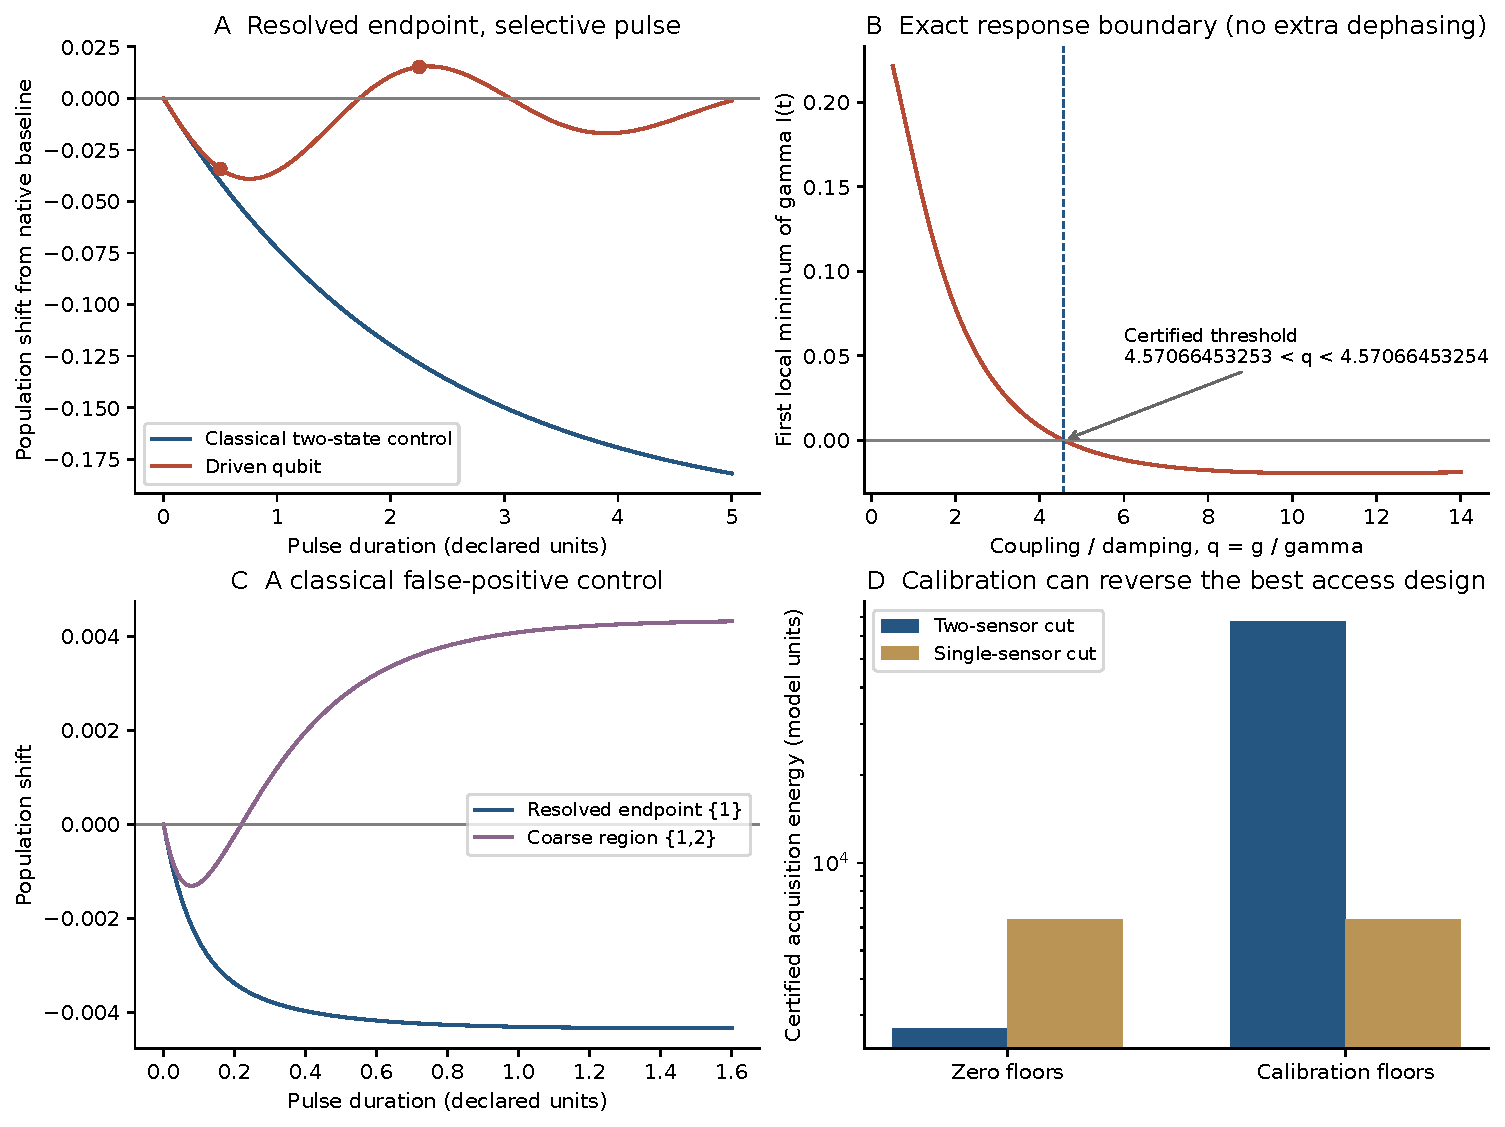
\includegraphics[width=\textwidth]{completion_results.pdf}
\caption{Four consequences of the declared access contracts. A: a driven qubit
crosses its native endpoint baseline, whereas its incoherent control does not.
B: the exact no-extra-dephasing response threshold separates the two regimes.
C: a coarse detector also crosses in a fully classical network; its resolved
endpoint remains protected. D: calibrated floors reverse the preferred current
sensor design at fixed certified accuracy. Curves illustrate proved models;
exact rational certificates, proofs and scope conditions accompany the release.
No panel represents measured experimental data.}
\label{completion:overview}
\end{figure}

\chapter{A preparation and randomized-readout assay}
\label{ch:rr-preparation}

The previous finite-pulse result used a stationary preparation and a selective
change to one physical transition channel.  Its positive first-hitting kernel
also supports a different experiment: prepare a detected state, compare it with
another preparation, and randomize the time of a single endpoint reading.  This
removes the stationary-preparation and selective-control requirements.  It
replaces them with a trusted reset and a common, time-homogeneous evolution.
Neither access contract is automatically easier to establish in an apparatus.

The mathematical result below is a Markov occupation maximum principle.
Converting it into an operational assay is useful, but it does not establish the
first test of arbitrary-size classical dynamics.  Established survival
inequalities already address closely related questions
\cite{rrLambert2010,rrLi2012,rrZhou2015}.  Section~\ref{sec:rr-comparison} compares
the present assay with those alternatives and records a baseline that outperforms
its simplest version.

\section{The classical preparation inequality}
\label{sec:rr-preparation-theorem}

Let $Q$ be a finite, time-homogeneous row generator and $P(t)=e^{tQ}$.
A reference arm prepares state $j$ exactly.  A comparison arm prepares a fixed
probability distribution $\rho$ over the same states.  Both arms evolve under
$Q$.  Independently of the trajectory and preparation arm, draw a readout time
uniformly from $[0,T]$, measured from preparation.  Record whether the system
occupies the singleton state $j$.

\begin{theorem}[Integrated return maximum]
\label{thm:rr-return}
For $i\ne j$ and $T>0$,
\begin{align}
 K_{ij}(T)
 &=\int_0^T\bigl(P_{jj}(t)-P_{ij}(t)\bigr)\,dt\nonumber\\
 &=\int_0^T P_{jj}(s)\Pr_i(\tau_j>T-s)\,ds>0,
 \label{eq:rr-hitting}
\end{align}
where $\tau_j$ is the first hitting time of $j$ from $i$.
Consequently, for every initial distribution $\rho$,
\begin{equation}
 C_{\rho,j}(T)
 =\frac1T\int_0^T\left(P_{jj}(t)-[\rho P(t)]_j\right)\,dt
 \ge0.
 \label{eq:rr-classical-null}
\end{equation}
The inequality is strict if $\rho_j<1$.  Irreducibility and a stationary
preparation are unnecessary.  If the exit rates from $i,j$ are at most
$\Lambda$, then $K_{ij}(T)/T\ge e^{-\Lambda T}$.
\end{theorem}

\begin{proof}
The strong Markov property at $\tau_j$ gives
\[
 P_{ij}(t)=\int_{[0,t]}P_{jj}(t-u)\Pr_i(\tau_j\in du).
\]
Integrating this identity and interchanging nonnegative integrals gives
\eqref{eq:rr-hitting}.  No departure from $j$ for $s$ time units has probability
at least $e^{-\Lambda s}$, and no departure from $i$ for $T-s$ units has
probability at least $e^{-\Lambda(T-s)}$.  These events give the claimed lower
bound and strict positivity.  Finally,
$T C_{\rho,j}=\sum_i\rho_iK_{ij}$, with $K_{jj}=0$.
\end{proof}

Only the reference preparation must be a trusted singleton.  The comparison
preparation may be an unknown fixed distribution.  This distinction matters for
calibration: uncertainty about that comparison distribution need not enlarge
the classical null, although it affects predicted power against a specified
alternative.  A computational-basis label in a quantum experiment does not by
itself establish a singleton classical hidden state.

A sufficient coarse-target extension is a genuine reset interface.  Let $B$ be
the detected set, with reference preparation $\nu_B$ supported in $B$ and a
comparison preparation outside $B$.  Suppose the conditional state at first
entry into $B$ is $\nu_B$, independently of the entry time and previous history.
The strong Markov argument then replaces $P_{jj}(s)$ by
$\Pr_{\nu_B}(X_s\in B)$ and proves the same inequality.  Mixtures of an outside
preparation with $\nu_B$ are also allowed.  Arbitrary states initially inside
$B$ are not covered by this sufficient condition.

\section{Protected clocks and failure controls}
\label{sec:rr-clocks}

\begin{theorem}[Decreasing readout densities]
\label{thm:rr-decreasing}
Let $w$ be a nonnegative, normalized, nonincreasing readout-time density on
$[0,\infty)$, shared by both preparations and independent of the dynamics.
Under Theorem~\ref{thm:rr-return},
\[
 \int_0^\infty w(t)
 \left(P_{jj}(t)-[\rho P(t)]_j\right)\,dt\ge0.
\]
Every such density is, up to null sets, a mixture of uniform densities:
\begin{equation}
 w(t)=\int_{[t,\infty)}\frac{\mu(dT)}{T},
 \qquad \mu(dT)=-T\,dw(T),
 \label{eq:rr-mixture}
\end{equation}
where $\mu$ is a probability measure.
\end{theorem}

\begin{proof}
For a decreasing integrable density, $t w(t)\to0$ at both endpoints.
Stieltjes integration by parts therefore gives
$\int\mu=\int_0^\infty w(t)\,dt=1$ and
$\int_{[t,\infty)}\mu(dT)/T=w(t)$, with endpoint conventions irrelevant to
probability densities.  Tonelli's theorem expresses the asserted contrast as
$\int C_{\rho,j}(T)\mu(dT)$, which is nonnegative by
Theorem~\ref{thm:rr-return}.  Equivalently, integration by parts against the
nonnegative cumulative kernel $K$ proves the sign directly.
\end{proof}

The mixture representation is established mathematics
\cite{rrPavlides2012}; its role here is to expose experimental timing choices.
Randomizing a cutoff $T$ and then drawing time uniformly in $[0,T]$ preserves
the inequality exactly.  For a specified alternative, no decreasing-density
clock can beat the best uniform horizon unless an additional constraint changes
the optimization problem.  Mean-time constraints, for example, lead to a
standard convex design problem.

The following controls show why the assumptions cannot be omitted.

\begin{enumerate}
\item \emph{A fixed or delayed readout can reverse the classical contrast.}
A directed three-cycle has $P_{jj}(t)<P_{ij}(t)$ at some times.  Its uniform
average over a delayed interval can also be negative.  Uniform sampling must
start at preparation.  Increasing time densities have no general guarantee.
\item \emph{A coarse detector can reverse the contrast.}
Take four states $j,i,k,a$, with rates $j\to a$ and $i\to k$ both equal to $2$,
and $a,k$ absorbing.  Detect $B=\{j,k\}$, prepare $j$ or $i$, and average over
$[0,1]$.  The contrast is
\[
 \int_0^1\bigl(2e^{-2t}-1\bigr)\,dt=-e^{-2}<0.
\]
This wholly classical model violates the singleton conclusion because entry
into $B$ does not reset to the reference state.
\item \emph{Scheduled dynamics can reverse the contrast.}
During $[0,1]$ allow only $j\to a$ at rate $4$; during $[1,2]$ allow only
$i\to j$ at rate $4$.  Preparing $j$ or $i$ and averaging the singleton-$j$
readout over $[0,2]$ gives
\[
 \frac12\left[\frac{2(1-e^{-4})}{4}+e^{-4}-1\right]<0.
\]
The generator is time dependent.  Augmenting the system with an internal clock
does not restore the required singleton or reset observation contract.
\end{enumerate}

Nonincreasing density is a sufficient condition, not a necessary
characterization of all safe clocks.  For example, placing at least half of the
readout probability at time zero protects the sign against any remaining
stochastic transition kernel.  The general clock cone is not characterized by
this work.  A rejection of the declared classical contract is not a
device-independent identification of quantum dynamics.

\section{A damped quantum model and an exact threshold}
\label{sec:rr-quantum}

Consider the valid qubit Lindblad generator
\begin{equation}
 \mathcal L(\rho)=-i\frac{\omega}{2}[X,\rho]
  +\gamma\left(\operatorname{Tr}(\rho)\frac I2-\rho\right),
 \qquad \omega>0,\quad\gamma\ge0.
 \label{eq:rr-qubit}
\end{equation}
The depolarizing term has Pauli jump operators
$\sqrt{\gamma/4}\,X$, $\sqrt{\gamma/4}\,Y$, and
$\sqrt{\gamma/4}\,Z$.
Prepare $j=|0\rangle$ or $i=|1\rangle$ and detect
$\Pi_j=|0\rangle\langle0|$.  The instantaneous contrast is
$e^{-\gamma t}\cos(\omega t)$, so uniform timing yields
\begin{equation}
 C(T)=\frac{\gamma+e^{-\gamma T}
       [-\gamma\cos(\omega T)+\omega\sin(\omega T)]}
       {(\gamma^2+\omega^2)T}.
 \label{eq:rr-qubit-contrast}
\end{equation}
For $\gamma=0$, this is $\sin(\omega T)/(\omega T)$.

\begin{theorem}[Orthogonal-preparation damping threshold]
\label{thm:rr-threshold}
For $\gamma>0$, a horizon with $C(T)<0$ exists if and only if
\begin{equation}
 \frac{\omega}{\gamma}\log\frac{\omega}{\gamma}>\frac{3\pi}{2},
 \quad\text{equivalently}\quad
 \frac{\omega}{\gamma}>e^{W(3\pi/2)}
 =3.644173671645632\ldots .
 \label{eq:rr-threshold}
\end{equation}
Here $W$ is the principal real Lambert function.  This threshold concerns
\eqref{eq:rr-qubit}, the stated orthogonal preparations, and the decreasing-clock
class.  It is not a universal coherence threshold.
\end{theorem}

\begin{proof}
Write $I(T)=T C(T)$.  Then $I'(T)=e^{-\gamma T}\cos(\omega T)$.
Its first local minimum following the initial maximum occurs at
$T_*=3\pi/(2\omega)$; subsequent minima occur one full period apart and have
values
\[
 I(T_n)=\frac{\gamma-\omega
 e^{-\gamma(3\pi/2+2\pi n)/\omega}}{\gamma^2+\omega^2},
 \qquad n=0,1,\ldots .
\]
These values increase with $n$.  Since $I(0)=0$, a negative value exists exactly
when $\omega e^{-3\pi\gamma/(2\omega)}>\gamma$.
Setting $r=\omega/\gamma$ gives $r\log r>3\pi/2$, whose unique root above one
is $e^{W(3\pi/2)}$.  The mixture theorem proves that decreasing clocks cannot
produce a reversal when every uniform horizon is nonnegative.
\end{proof}

When reversal exists, the most negative uniform contrast occurs within
$(\pi/\omega,3\pi/(2\omega))$.  Indeed
$C'(T)=[T I'(T)-I(T)]/T^2$, and the numerator is strictly increasing throughout
that interval because its derivative is $T I''(T)>0$.  It changes sign between
the first zero of $I$ and its first negative minimum.  Later periods increase
a negative numerator $I$ toward its positive limiting value while also increasing
$T$, so they cannot improve the negative average.

With $\gamma=1/10$, $\omega=2$, $T=9/4$, and a common affine detector of gain
$9/10$, the observed contrast is
\[
 C_{\rm obs}=-0.1440713137250376\ldots<-\frac{18}{125}.
\]
The strict rational inequality is certified by an $80$-degree Taylor enclosure,
independent of floating-point agreement.  Mean evolution time is $9/8$ per
record.  Preparation, readout, reset, and control energy remain separate costs.
An exponentially distributed readout with rate $\lambda$, by contrast, yields
\[
 C_{\exp}=\frac{\lambda(\lambda+\gamma)}
                 {(\lambda+\gamma)^2+\omega^2}>0.
\]
It respects the classical protection but has no power against this alternative.

\section{The best comparison preparation}
\label{sec:rr-spectral-preparation}

For a quantum channel semigroup $\Phi_t$ and a trusted reference state $|j\rangle$,
define the averaged accessible effect
\[
 A_T=\frac1T\int_0^T\Phi_t^\dagger(\Pi_j)\,dt.
\]
The reference score is $\langle j|A_T|j\rangle$; arbitrary quantum state
preparation attains the maximal score $\lambda_{\max}(A_T)$.  The Rayleigh
variational principle therefore gives the optimal reversal gap
\begin{equation}
 V_T=\lambda_{\max}(A_T)-\langle j|A_T|j\rangle.
 \label{eq:rr-spectral-gap}
\end{equation}
This is established spectral optimization applied to experimental design, not a
new eigenvalue theorem.  A nonzero matrix element connecting $j$ to its
orthogonal subspace guarantees $V_T>0$.

For \eqref{eq:rr-qubit}, write
\begin{align*}
 C&=\frac1T\int_0^T e^{-\gamma t}\cos(\omega t)\,dt,\\
 S&=\frac1T\int_0^T e^{-\gamma t}\sin(\omega t)\,dt
 =\frac{\omega-e^{-\gamma T}
 [\omega\cos(\omega T)+\gamma\sin(\omega T)]}
 {(\gamma^2+\omega^2)T}.
\end{align*}
Then $A_T=(I+C Z+S Y)/2$ for the Hamiltonian convention in
\eqref{eq:rr-qubit}, and
\[
 V_T=\frac{\sqrt{C^2+S^2}-C}{2}.
\]
For $\gamma>0$, the integrated sine $S$ is positive at every $T>0$: successive
positive sine lobes precede their negative partners and carry larger exponential
weight.  Within a negative lobe the smallest accumulated value is its endpoint,
where that paired contribution remains positive.  Thus $V_T>0$ for every
$\gamma,\omega,T>0$ when the comparison state can be coherently optimized.
This does not promise useful precision under arbitrarily strong damping;
for fixed $T$ and $\gamma\gg\omega$, the gap scales approximately as
$\omega^2/(4\gamma^3T)$.

A fixed $+Y$ eigenstate is often nearly optimal and avoids a model-dependent
preparation angle.  Its gap is $(S-C)/2$.  At $\gamma=1/10$, $\omega=2$,
$T=7/4$, and detector gain $9/10$, exact rational enclosures give
\[
 V_{+Y,\rm obs}=0.257271133487835\ldots>\frac{257}{1000}.
\]
Mean evolution time is $7/8$.  Coherent comparison preparation is an additional
physical resource, and already presumes the relevant coherent controls; this
example is not evidence for device-independent quantum certification.

\section{Calibration and established experimental baselines}
\label{sec:rr-comparison}

A common fixed binary detector with response $m(p)=d_0+k p$, $k>0$, preserves
the classical sign and cancels its offset.  Reference-preparation total-variation
error $\epsilon_j$ weakens the classical null by at most $\epsilon_j$.
Comparison-preparation error is unnecessary for that null when any initial
distribution is allowed, but contributes to predicted alternative power.
A common readout-law discrepancy of total variation $\delta$ changes a contrast
by at most $2\delta$.  Separate detector probability errors add their two radii.
A joint calibrated record-law bound should replace, rather than duplicate,
errors already accounted for individually.  Statistical confidence cannot
establish the reset or clock assumptions from the same test records.

A close prior comparator is the survival inequality
\cite{rrLambert2010}
\[
 |2P_{jj}(t)-P_{jj}(2t)|\le1.
\]
The classical semigroup actually gives the stronger relation
\begin{equation}
 P_{jj}(2t)=\sum_kP_{jk}(t)P_{kj}(t)\ge P_{jj}(t)^2.
 \label{eq:rr-survival-product}
\end{equation}
The usual upper inequality follows from $2p-p^2\le1$.  To estimate
\eqref{eq:rr-survival-product} directly, multiply the binary outcomes of two
independent length-$t$ records and compare that product with a length-$2t$
record.  The product is Bernoulli with mean $P_{jj}(t)^2$ and consumes two
physical preparations.

For a linear contrast $\sum_k a_k p_k$ with positive alternative gap $g$, a
common sufficient Hoeffding design has resource proxy
\begin{equation}
 \mathcal B=\frac{\left(\sum_k |a_k|\sqrt{c_k}\right)^2}{g^2},
 \label{eq:rr-hoeffding-proxy}
\end{equation}
where $c_k$ is the resource cost of one independent observation of arm $k$.
The same confidence factor multiplies this proxy for all methods.  This is a
comparison of sufficient concentration-bound designs, not their exact minimum
sample complexities.  For randomized clocks, evolution-time cost below means
\emph{expected} evolution time; it is not a hard bound on elapsed laboratory
time or a measurement of energy.

Table~\ref{tab:rr-baselines} fixes $\gamma=0.1$, $\omega=2$, ideal known readout,
independent records, and zero preparation overhead.  Each column optimizes its
own time parameter numerically on $[0.001,5]$.  Physical record costs for the
product arm include both preparations.  The coherent-preparation variants use
an additional control resource.

\begin{table}[htbp]
\centering
\begin{tabular}{lrr}
\hline
Method & Record proxy & Expected-time proxy\\
\hline
Uniform clock, orthogonal preparation &156.08&174.02\\
Established linear survival inequality &219.68&133.64\\
Classical survival-product inequality &75.84&58.02\\
Uniform clock, fixed quadrature preparation &48.81&40.15\\
Uniform clock, optimized preparation &48.39&40.02\\
\hline
\end{tabular}
\caption{Matched sufficient-bound comparisons.  Lower is better.  These are
numerical design results, not physical measurements or certified global
statistical optima.  The survival-product baseline beats the simplest new
assay; extra coherent preparation changes the available operations.}
\label{tab:rr-baselines}
\end{table}

The comparison rejects a claim of universal superiority for the randomized
assay.  Its contribution is a different exact access contract, protected timing
families, and a route to calibrated design.  Which method is experimentally
preferable depends on preparation access, detector errors, timing, and actual
apparatus costs.  A framework becomes more useful when it selects among these
methods and records their failure cases, not when it relabels every modeled
quantum signal as a breakthrough.

\section{Preparation design for a baseline-subtracted dimension witness}
\label{sec:rr-baseline-preparation}

The dimension result developed later, Proposition~\ref{rr:dimension-robust},
changes the null assumptions again.  For a homogeneous CTMC with at most three
hidden states, it permits arbitrary fixed preparations $\mu,\nu$ and an
arbitrary fixed stochastic detector $f\in[0,1]$.  Writing
\[
 C_0=(\mu-\nu)f,\qquad
 C_T=(\mu-\nu)\frac1T\int_0^T e^{tQ}f\,dt,
\]
its bound is $|C_0-C_T|\le1$.  Separately measuring the two preparations at
baseline and at randomized time therefore removes the exact hidden-reset
assumption of the earlier assay, at the price of a restriction on classical
hidden-state dimension.  Section~\ref{rr:four-states} exhibits the importance
of that restriction.  The quantum design calculation is independent of the
proof of the classical bound.

\begin{lemma}[Quantum preparation design for the dimension witness]
\label{lem:rr-dimension-preparation}
For a quantum averaged effect $A_T$ and the same baseline effect $\Pi_j$, let
$D_T=\Pi_j-A_T$.  The largest value of
\[
 W=\operatorname{Tr}\!\left[D_T(\rho_+-\rho_-)\right]
\]
over two arbitrary quantum preparations is the spectral diameter
$\lambda_{\max}(D_T)-\lambda_{\min}(D_T)$.
For the qubit model \eqref{eq:rr-qubit}, it is
\begin{equation}
 W_{\max}(T)=\sqrt{(1-C)^2+S^2},
 \label{eq:rr-dimension-optimum}
\end{equation}
attained by antipodal pure Bloch vectors parallel to $(0,-S,1-C)$.
\end{lemma}

\begin{proof}
The maximum and minimum expectations of a Hermitian matrix are its largest and
smallest eigenvalues, independently attainable by the two preparations.
Here $D_T=[(1-C)Z-SY]/2$, whose eigenvalues are
$\pm\sqrt{(1-C)^2+S^2}/2$.
\end{proof}

This is a standard spectral variational calculation used for experimental
selection.  Orthogonal $Z$ preparations instead give $W=1-C$, whose optimal
horizon is exactly the most negative uniform contrast studied above.  A common
affine detector of gain $k$ multiplies these modeled quantum contrasts by $k$.
For those orthogonal preparations, a predicted violation requires
$k>1/(1-C)$.  The classical dimension bound itself does \emph{not} require this
affine detector model or a known positive gain: it already permits any fixed
stochastic $f$.  Gain enters prediction of experimental power, not validity
of that null.

A simple rational preparation gives a larger certified margin than the
orthogonal pair.  Set
\[
 \gamma=\frac1{10},\quad\omega=2,\quad T=2,\quad k=\frac9{10},
 \qquad n=\left(0,-\frac{12}{37},\frac{35}{37}\right).
\]
The vectors $n$ and $-n$ are pure because $12^2+35^2=37^2$.  Exact rational
Taylor enclosures certify
\begin{equation}
 W=k\left[\frac{35}{37}(1-C)+\frac{12}{37}S\right]
 =1.0806050936582667\ldots>\frac{27}{25}.
 \label{eq:rr-rational-dimension-witness}
\end{equation}
Each randomized-time arm has mean evolution time $1$; each baseline arm has
zero evolution time in the ideal timing convention.  Four equally sampled
arms therefore have mean evolution time $1/2$ per physical record.  All four
arms still incur preparation, measurement, and reset costs.  A common
uncontrolled readout delay must be included consistently in the baseline and
random-time effects; it is not automatically covered by the zero-delay
alternative prediction above.

Numerical optimization gives an ideal-state value about $1.20123$ at
$T\simeq2.04524$ for this damping and frequency, or $1.08111$ after gain $0.9$.
The rational design is close to that numerical value, but the reported search
is not a certificate of a global optimum.  Established dimension witnesses and
survival tests remain relevant comparators.  The present result is an explicit
physical alternative and a reproducible preparation choice for the stated
finite-dimension null, not an unrestricted exclusion of classical hidden
mechanisms.

\chapter{A sharp boundary for hidden classical explanations}
\label{rr:reset-boundary}

A response reversal can establish that a declared experimental model is
inadequate without identifying its replacement. Hidden detector states,
imperfect preparation, and uncharacterized crossing rates can all matter.
This chapter turns two of those alternatives into quantitative requirements.
Its main result interpolates sharply between a protected regenerative interface
and unrestricted coarse observation. It is a theorem about specified stochastic
models, with no assumption of historical priority or empirical confirmation.

\section{The measured quantity and the physical assumptions}

Let $R$ be a finite continuous-time Markov generator and $B$ a detector region.
An initial distribution $\nu_A$ is supported outside $B$ and $\nu_B$ inside $B$.
For any initial distribution $\nu$, define
\[
 U_\nu(T)=\int_0^T\Pr_\nu(X_s\in B)\,ds,
 \qquad H(T)=U_{\nu_B}(T)-U_{\nu_A}(T).
\]
The normalized contrast $H(T)/T$ is directly observable by preparing either
initial distribution and reading the same binary detector at an independently
chosen uniform time in $[0,T]$. This formulation requires neither stationary
preparation nor a current measurement. Preparation errors and detector errors
must still be propagated into the contrast interval.

In the stationary selective-channel experiment developed earlier, the same
quantity enters through
\[
 D_B(T)=[\pi e^{TR}](B)-\pi(B)=\gamma H(T),
 \qquad \pi R=\gamma(\nu_B-\nu_A).
\]
Thus the present result can also interpret a finite-pulse response, provided the
forcing identity and any division by $\gamma$ have been separately justified.
The direct preparation experiment and this response-based experiment are
separate access contracts.

We assume uniform \emph{crossing-hazard} bounds
\begin{equation}
 \sum_{y\in B}R_{xy}\leq a\quad(x\notin B),\qquad
 \sum_{y\notin B}R_{xy}\leq b\quad(x\in B).
 \label{rr:hazards}
\end{equation}
These are bounds on every relevant hidden state, not averages inferred from
steady occupancy. Rates of motion within either detector region need not be
bounded. In particular, a proposed classical hidden-state model is not entitled
to use only the dissipative jump rates of a Lindblad description as its hazard
caps: that substitution would itself need physical justification.

Let $\tau$ be the first entrance into $B$ starting from $\nu_A$. Write $\mu$ for
the possibly defective distribution of $\tau$ and $\zeta_u$ for the entrance
state distribution conditional on $\tau=u$. A reset-defect bound $\eta$ means
\begin{equation}
 \operatorname{TV}(\zeta_u,\nu_B)\leq\eta,
 \qquad \mu\text{-almost every }u\leq T,
 \qquad 0\leq\eta\leq1.
 \label{rr:reset-defect}
\end{equation}
The conditioning on entrance time is substantive. An unconditional average
entrance distribution does not establish this condition. When $\nu_B$ is the
single state $j$, the defect at time $u$ is precisely the conditional probability
of entering through a different hidden state. A nonzero defect can arise in a
perfectly Markovian classical model; it is not synonymous with non-Markovianity.

\section{A sharp hazard--reset tradeoff}

For $c\geq0$ set
\[
 A_c(T)=\begin{cases}(1-e^{-cT})/c,&c>0,\\T,&c=0,\end{cases}
\]
and define
\begin{align}
 G_{a,b}(T)&=\int_0^T e^{-bs-a(T-s)}\,ds,\label{rr:G}\\
 K_{a,b}(T)&=T-A_a(T)-A_b(T)+G_{a,b}(T).\label{rr:K}
\end{align}
Here $G_{a,a}(T)=Te^{-aT}$ and, for $a\ne b$,
$G_{a,b}(T)=(e^{-aT}-e^{-bT})/(b-a)$.

\begin{theorem}[Sharp coarse-detector response bound]
\label{rr:sharp-reset}
Under \eqref{rr:hazards} and \eqref{rr:reset-defect},
\begin{equation}
 H(T)\ \geq\ G_{a,b}(T)-\eta K_{a,b}(T)
 =(1-\eta)G_{a,b}(T)+\eta\{A_a(T)+A_b(T)-T\}.
 \label{rr:sharp-bound}
\end{equation}
The lower bound is attained by a finite classical Markov model for every
$a,b>0$, $T>0$, and $\eta\in[0,1]$.
\end{theorem}

\begin{proof}
Write $p_B(s)=\Pr_{\nu_B}(X_s\in B)$ and
$S(u)=\Pr_{\nu_A}(\tau>u)$. The strong Markov property gives
\[
 U_{\nu_A}(T)=\int_{[0,T]}U_{\zeta_u}(T-u)\,\mu(du).
\]
Adding and subtracting the same expression with $\zeta_u$ replaced by $\nu_B$
yields the exact decomposition
\begin{align*}
 H(T)&=G_{\rm actual}(T)-\mathcal R(T),\\
 G_{\rm actual}(T)&=\int_0^T p_B(s)S(T-s)\,ds,\\
 \mathcal R(T)&=\int_{[0,T]}
       [U_{\zeta_u}(T-u)-U_{\nu_B}(T-u)]\,\mu(du).
\end{align*}
The hazard caps imply $p_B(s)\geq e^{-bs}$ and $S(u)\geq e^{-au}$ by
considering trajectories that have not yet left their initial region.
Consequently $G_{\rm actual}(T)\geq G_{a,b}(T)$.

For every initial state $x\in B$,
$A_b(v)\leq U_x(v)\leq v$. Total variation therefore bounds the reset term by
\[
 \mathcal R(T)\leq
 \eta\,\mathbb E[(T-\tau)_+-A_b((T-\tau)_+)].
\]
The function $v-A_b(v)$ is nonnegative and increasing. Since the entrance
hazard is at most $a$, $\tau$ stochastically dominates an exponential variable
of rate $a$; mass at $\tau=\infty$ contributes zero. For $a>0$, the last
expectation is at most
\begin{align*}
 \int_0^T ae^{-au}[T-u-A_b(T-u)]\,du
 &=\int_0^T[1-e^{-a(T-s)}][1-e^{-bs}]\,ds\\
 &=K_{a,b}(T).
\end{align*}
The formula extends continuously to $a=0$ or $b=0$, when $K=0$.
These estimates prove the inequality.

For attainment, use four states $i,j,k,\ell$, detector $B=\{j,k\}$,
$\nu_A=\delta_i$, $\nu_B=\delta_j$, and the only transitions
\[
 i\longrightarrow j:\ a(1-\eta),\qquad
 i\longrightarrow k:\ a\eta,\qquad
 j\longrightarrow\ell:\ b.
\]
States $k$ and $\ell$ are absorbing. The entrance time is exponential with
rate $a$ and its independent entrance law is
$(1-\eta)\delta_j+\eta\delta_k$. Moreover,
$U_j(v)=A_b(v)$ and $U_k(v)=v$. Every inequality above is an equality.
\end{proof}

The small-time defect penalty is
$K_{a,b}(T)=abT^3/6+O(T^4)$, whereas
$G_{a,b}(T)=T-(a+b)T^2/2+O(T^3)$.
The bounds are therefore sensitive to the time available for both entrance and
exit. The sharpness claim concerns the stated class, not the precision attainable
at fixed energy on an unspecified apparatus.

For $0<\eta<1$, the same bound is the infimum within irreducible models
compatible with the stationary selective-channel experiment. To see this,
add $j\to i$, $k\to j$, and $\ell\to i$ at rate $\varepsilon$, and replace
$j\to\ell$ by $b-\varepsilon$. For sufficiently small positive $\varepsilon$,
the chain is irreducible, both hazard caps and the entrance-reset law remain
unchanged, and its kernel tends to the attaining kernel. Double the two
$i\leftrightarrow j$ rates to define the native generator $Q$. It has a positive
stationary law $\pi$, and suppressing that channel by one half returns $R$.
The response identity is then exact. The native current tends to zero in this
limit; approximate sharpness does not confer a finite-sample advantage for
measuring a shrinking current.

\section{Comparison preparations that already occupy the detector}

The outside-support condition cannot be inferred from a preparation's name or
from an analogy with a qubit basis. Suppose instead that the comparison state is
\[
 \rho=p\nu_{\rm in}+(1-p)\nu_{\rm out},\quad
 \operatorname{supp}\nu_{\rm in}\subseteq B,\quad
 \operatorname{supp}\nu_{\rm out}\subseteq B^c,
\]
with $\operatorname{TV}(\nu_{\rm in},\nu_B)\leq\eta_0$. Let the first-entrance
reset defect from $\nu_{\rm out}$ be bounded by $\eta_1$.
\begin{proposition}[Sharp mixed-preparation extension]
Under the same hazard caps,
\[
 U_{\nu_B}(T)-U_\rho(T)\geq
 (1-p)\{G_{a,b}(T)-\eta_1 K_{a,b}(T)\}
 -p\eta_0\{T-A_b(T)\}.
\]
\end{proposition}
\begin{proof}
Decompose the contrast into its inside and outside contributions. Apply the
previous theorem to the outside contribution and
$U_{\nu_B}-U_{\nu_{\rm in}}\geq-\eta_0(T-A_b)$ to the inside contribution.
The same four-state extremizer, with entrance mixture parameter $\eta_1$ and
$\nu_{\rm in}=(1-\eta_0)\delta_j+\eta_0\delta_k$, attains the result.
\end{proof}
With no reset assumptions, $\eta_0=\eta_1=1$, the sharp bound simplifies to
\[
 U_{\nu_B}(T)-U_\rho(T)\geq A_b(T)+(1-p)A_a(T)-T.
\]
This expression also follows directly from conditional crossing-hazard survival
and therefore has the broader classical-process scope described next. If only
an upper bound on $p$ is known, use that upper bound. For $p=1$ there need not be
any positive protection interval. A preparation with one-half detector
occupancy must not be analyzed using the $p=0$ formula.

\section{An explanation bound without a protected reset assumption}

Setting $\eta=1$ removes the reset assumption entirely:
\begin{equation}
 H(T)\geq A_a(T)+A_b(T)-T.
 \label{rr:unrestricted-coarse}
\end{equation}
This special case has a still broader interpretation. Consider any classical
binary process with the stated initial detector value and with uniformly bounded
conditional crossing intensities: at most $a$ from outside to inside and at most
$b$ in the reverse direction, under every admissible history. Survival before
the first crossing obeys the same exponential bounds. At each time $s$,
\[
 \Pr_{\nu_B}(B,s)\geq e^{-bs},\qquad
 \Pr_{\nu_A}(B,s)\leq1-e^{-as}.
\]
Integration proves \eqref{rr:unrestricted-coarse}. No finite hidden dimension,
Markov property, stationarity, or specified first-entrance reset is needed for
this case. The hypothesis of finite uniformly bounded crossing intensities
remains essential; deterministic jumps and unbounded boundary chatter do not
satisfy it.

With a common cap $a,b\leq\lambda$, define
\[
 F(z)=\frac{2(1-e^{-z})}{z}-1,\qquad F(0)=1.
\]
Then $H(T)/T\geq F(\lambda T)$. The function $F$ decreases strictly from $1$
to $-1$. Its zero is $z_0=1.593624260\ldots$, defined exactly by
$z_0=2(1-e^{-z_0})$. Hence an integrated contrast cannot become negative before
$T=z_0/\lambda$, regardless of the number of hidden classical states. The
supplied rational certificates place $z_0$ strictly between $1.593$ and $1.594$.

This result can be used without pretending that a classical hazard cap has
already been experimentally certified. If $c_U\in(-1,1)$ is a calibrated upper
confidence bound on $H(T)/T$, every classical explanation with finite conditional
crossing intensities must have
\begin{equation}
 \lambda\geq\frac{F^{-1}(c_U)}{T}.
 \label{rr:activity-inverse}
\end{equation}
This is a lower bound on the peak crossing intensity required of that explanation.
It becomes a rejection test only when an independently justified upper cap is
smaller. Observing a negative contrast by itself neither excludes all classical
models nor establishes a thermodynamic energy cost for their activity.

\section{What finite data can establish}

Under calibrated caps $a,b$ with $K_{a,b}(T)>0$, an upper confidence bound $H_U$
on $H(T)$ implies
\begin{equation}
 \eta\geq\max\left\{0,
       \frac{G_{a,b}(T)-H_U}{K_{a,b}(T)}\right\}.
 \label{rr:defect-inverse}
\end{equation}
A value exceeding one is inconsistent with the declared bounded-hazard
classical contract. A positive value below one states a minimum required reset
defect. It does not identify which microscopic state or physical mechanism
caused that defect. If $K=0$, the response bound is independent of $\eta$ and
one must test that bound directly instead of dividing by zero.

For a simple direct protocol, collect $N$ independent binary observations from
each initial preparation, choosing the observation time independently and
uniformly in $[0,T]$ for every record. Let $\widehat c$ be the difference of the
two empirical means in the order $B$ minus $A$. Weighted Hoeffding gives
\[
 \Pr\{H(T)/T>\widehat c+u\}\leq e^{-Nu^2}
\]
under the ideal model. If separately calibrated per-arm record laws differ in
total variation by at most $\epsilon_B$ and $\epsilon_A$, use
$c_U=\widehat c+u+\epsilon_B+\epsilon_A$. A joint calibration failure allowance
is added once. The bound assumes independent records and predetermined sample
counts; adaptive stopping requires a valid sequential procedure. The exact
binomial procedure in the statistical chapter offers a complementary encoded
single-bit implementation.

The software implements the sharp bound and its inversions with rational
exponential enclosures. An output certificate establishes a conditional
mathematical statement, not the correctness of the supplied hardware
calibration. The hazard-inversion helper gives both endpoints of a certified
root bracket. It does not report the numerical root as an exact physical rate.

\section{A sharp four-state requirement without a hazard calibration}
\label{rr:four-states}

The geometry of a binary detector gives an additional explanation bound that
does not require a kinetic cap or a protected reset interface.
\begin{theorem}[Minimum classical state count for a negative integrated contrast]
\label{rr:dimension}
Consider a common finite, time-homogeneous classical Markov generator, a fixed
binary detector region $B$, and initial distributions supported respectively
inside and outside $B$. If the hidden state space has at most three states,
then $H(T)>0$ for every finite $T>0$. Thus $H(T)<0$ requires at least four
classical Markov states. Four states suffice to realize any prescribed value
$H(T)/T\in(-1,0)$ at a prescribed positive $T$.
\end{theorem}
\begin{proof}
Both detector regions are nonempty. With at most three states, one of them is a
singleton. If $B=\{j\}$, the first-hitting return argument gives
\[
 U_j(T)-U_{\nu_A}(T)
 =\int_0^T P_j(X_s=j)\Pr_{\nu_A}(\tau_j>T-s)\,ds>0.
\]
The inequality is strict because a finite generator permits positive no-jump
probabilities at every finite time. If instead $B^c=\{i\}$, complement the
detector:
\[
 U^B_{\nu_B}(T)-U^B_i(T)
 =U^{B^c}_i(T)-U^{B^c}_{\nu_B}(T)>0,
\]
and apply the same argument. This covers arbitrary mixtures within the allowed
initial supports.

For sufficiency, use the four-state attaining model with $\eta=1$ and
$a=b=\lambda$. Its contrast is $F(\lambda T)$, which decreases continuously
from $1$ to $-1$. Every specified contrast in $(-1,0)$ therefore determines a
unique positive $\lambda$ and is attained exactly.
\end{proof}

The matching claim concerns one integrated contrast. Four states need not
reproduce the full time-resolved record, multiple intervention responses, or
a complete quantum process. State count also does not determine stationary
Shannon entropy, physical memory cost, or thermodynamic dissipation.

A qubit supplies a direct mathematical comparison. Under unitary evolution
with Hamiltonian $gX$, initial states $|1\rangle$ and $|0\rangle$, and detector
$|1\rangle\langle1|$, the contrast is
\[
 \frac{H(T)}{T}=\frac{\sin(2gT)}{2gT}.
\]
At $T=3\pi/(4g)$ it equals $-2/(3\pi)$. A two-dimensional quantum system can
therefore produce a contrast that requires at least four states in the stated
classical Markov representation. This is a conditional state-count separation,
not a device-independent proof of quantumness or a claim that classical
four-state models are inadequate for that scalar observation.

\begin{proposition}[A conservative preparation-robust state-count witness]
\label{rr:dimension-robust}
Allow a fixed stochastic binary detector with response $f(x)\in[0,1]$ and
arbitrary initial preparations $\nu_B,\nu_A$. Write
\[
 m_B=\nu_B f,\quad m_A=\nu_A f,\quad
 C_f(T)=\frac1T\int_0^T(\nu_B-\nu_A)e^{sR}f\,ds.
\]
Write $C_0=m_B-m_A$. Every homogeneous classical model with at most three
states satisfies the directly observable bound
\begin{equation}
 \boxed{\left|C_0-C_f(T)\right|\leq1.}
 \label{rr:dimension-drop}
\end{equation}
In particular,
\begin{equation}
 C_f(T)\geq m_B-m_A-1.
 \label{rr:dimension-noise}
\end{equation}
\end{proposition}
\begin{proof}
First consider a deterministic detector region $D$. Conditional preparations
inside and outside $D$ have nonnegative integrated contrast by the preceding
theorem. Replacing the actual preparations by these conditional preparations
changes a normalized occupation expectation by at most
$\nu_B(D^c)+\nu_A(D)$ in total. If a conditional preparation is undefined, this
sum is at least one and the bound follows from the range $[-1,1]$.
Thus the normalized contrast for $D$ is at least
$-\nu_B(D^c)-\nu_A(D)$.

Use the layer-cake representation
$f(x)=\int_0^1\mathbf1_{\{f(x)>u\}}\,du$ and integrate that bound over the
threshold detector regions. The two integrated impurity terms are
$1-\nu_B f$ and $\nu_A f$, proving \eqref{rr:dimension-noise}. Swapping the
two preparations proves the opposite bound and hence
\eqref{rr:dimension-drop}.
\end{proof}

The bound in \eqref{rr:dimension-drop} is sharp as a supremum for the
three-state class. Let a reference state be absorbing with detector response
$c\in[0,1]$. Let the comparison state have detector response zero and jump at
rate $\lambda$ to a third absorbing state with detector response one. Then
$C_0=c$, $C_f(T)=c-1+A_\lambda(T)/T$, and
$C_0-C_f(T)=1-A_\lambda(T)/T\to1$ as $\lambda\to\infty$.
The more specific impurity form is not claimed optimal for every separately
specified pair of initial means.

With simultaneous confidence
bounds $C_U$, $m_{B,L}$, and $m_{A,U}$, the condition
\[
 C_U<m_{B,L}-m_{A,U}-1
\]
excludes every classical model with at most three homogeneous Markov states
under the fixed-detector contract. It requires no statement that either
preparation has exactly zero hidden impurity. The same observable bound applies to every independent nonincreasing
observation-clock density starting at zero. The clock chapter represents such
a density as a mixture of uniform clocks, so
\[
 C_w=\int C_f(T)\,\mu(dT),\qquad
 |C_0-C_w|\leq\int|C_0-C_f(T)|\,\mu(dT)\leq1.
\]
A clock chosen using the evolving hidden trajectory is not covered by this
argument.

The directly observable score $C_0-C_f(T)$ needs no assumption of exactly
pure hidden preparations. It requires the same detector response function at
baseline and at the random observation time, and the same preparations in the
corresponding arms. Common fixed readout noise is already covered by
$f\in[0,1]$. If a detector is permitted to reverse its labels between baseline
and readout, a motionless two-state system can give $C_0=1$ and $C_f(T)=-1$;
readout stability is therefore essential.

A common known delay $d$ before both baseline and random-time observations does
not invalidate \eqref{rr:dimension-drop}. Replace the preparations by
$\nu_B e^{dR}$ and $\nu_A e^{dR}$, which are allowed to be arbitrary. The same
argument covers an independent common delay distribution used in every arm,
by averaging these effective preparations; the delay must also be independent
of the observation-clock draw. Different delay distributions,
changed generators, or different detector calibrations require separate error
bounds.

The four-state equal-hazard construction can match both averaged arm
probabilities of a unital qubit with orthogonal preparations and a projective
binary detector: they are $A_\lambda(T)/T$ and $1-A_\lambda(T)/T$, equivalently
$(1+C)/2$ and $(1-C)/2$ once $F(\lambda T)=C$. This statement applies when the
random timestamps are discarded. Keeping the timestamp, intervening within
records, or comparing several clocks yields additional data that the scalar
matching argument does not reproduce.

Time homogeneity is essential. A three-state classical counterexample starts
in $j$ or $i$ with detector $\{j\}$. First allow $j\to k$ at rate ten for time
$1/10$; next allow $i\to j$ at rate ten for time $1/10$; then freeze all rates
for time one. The integrated contrast over the whole interval is
\[
 H(6/5)=\frac{19}{10e}-\frac9{10}<0.
\]
Thus an external control clock, unmodeled memory, or preparation-dependent
kinetics can invalidate the state-count conclusion. The theorem compares
common autonomous Markov representations; these restrictions must be checked
before interpreting the result as a hidden-state requirement.

\section{Protected graph interfaces beyond one entrance gateway}

For a known directed support graph, additional protections are available without
numerical rate identification. Write $U_x(T)$ for the occupation integral from
state $x$. Two elementary first-hitting comparisons hold for every rate choice:
\begin{enumerate}
\item If $x\in B$ and every directed path from $x$ to $B^c$ visits $y$, then
      $U_x(T)\geq U_y(T)$.
\item If $y\notin B$ and every directed path from $y$ to $B$ visits $x$, then
      $U_x(T)\geq U_y(T)$.
\end{enumerate}
For the first, all time before hitting $y$ is spent in $B$, and
$U_y(T)-U_y(T-s)\leq s$. For the second, no time before hitting $x$ is spent in
$B$, and $U_x$ is increasing. The strong Markov property gives each comparison,
including trajectories that never reach the gateway.

These inequalities compose transitively. A reachability test after deleting a
candidate gateway checks every primitive, and transitive closure supplies a
verifiable chain of comparisons. For example, on the graph
$i\to k$, $k\to\ell$, $j\to k$, $\ell\to k$ with $B=\{j,k\}$,
neither $j$ as the entrance gateway from $i$ nor $i$ as the exit gateway from
$j$ is valid. Nevertheless $U_j\geq U_k\geq U_i$. A closed detector region is
also protected by the exit condition. The implemented preorder is a sufficient
certificate. A complete graph characterization of universal occupation order
is not claimed, and failure to find a certificate is not evidence of a
counterexample.

\section{Why exact hidden structure cannot be certified by finite records}

A finite calibration experiment cannot uniformly rule out arbitrarily weak
unmodeled transitions. Suppose extra transitions have total intensity at most
$\delta$ at every state and under every allowed control. Coupling the original
and perturbed processes until the first extra jump gives, for records with total
pathwise horizon at most $L$,
\[
 \operatorname{TV}(P_{\rm original},P_{\rm perturbed})
 \leq1-e^{-\delta L}\leq\delta L.
\]
This statement includes adapted controls that obey the same intensity bound;
any detector or downstream processing preserves the inequality. Consequently,
a finite-record rule that accepts the original structural explanation with
probability $p$ accepts a sufficiently small perturbation with probability at
least $p-\delta L$.

The issue can affect all-time protection, not merely exact graph labels. Take
$i\to k$ at rate one and $j\to\ell$ at rate $\delta$, with
$B=\{j,k\}$ and $k,\ell$ absorbing. At $\delta=0$,
$H(T)=1-e^{-T}>0$ for every positive $T$. At every $\delta>0$,
\[
 H(T)=A_\delta(T)+A_1(T)-T
\]
eventually becomes negative, while finite-horizon records approach those of
the protected model as $\delta\downarrow0$. Structural physical knowledge,
a quantitative tolerance, or a positive separation assumption is therefore
needed. Taking additional finite records alone cannot establish exact absence
of all arbitrarily weak hidden alternatives.

The practical output is an explicit choice: certify a physical interface,
report a quantitative minimum reset defect, or report the hidden peak crossing
intensity any competing classical explanation would require. Each result says
what the evidence establishes and what remains open.

\chapter{Designing a protected random observation clock}
\label{rr:clock}

Timing is part of experimental access. A fixed-time population comparison can
have either sign in a classical network, while its uniform average starting at
preparation has a protected sign. This chapter describes clocks that retain
that guarantee and makes a limited resource-design problem exactly solvable.
The mixture representation and linear-programming geometry are established
mathematical tools; their use here does not assert new generic optimization
theory.

\section{Decreasing densities are mixtures of uniform clocks}
For a protected classical reset state $j$ and any other initial distribution
$\rho$, write
\[
 f(t)=P_j(X_t=j)-P_\rho(X_t=j),\qquad
 H(T)=\int_0^T f(t)\,dt\geq0.
\]
The same statement applies to a region with the required regenerative reset
property. A clock is drawn independently of the physical trajectory, with a
common probability density $w$ for both preparations. Its contrast is
$C_w=\int_0^\infty w(t)f(t)\,dt$.

\begin{proposition}[A constructive protected clock class]
Every nonincreasing probability density on $[0,\infty)$ is, up to changes on
a set of measure zero, a mixture of uniform densities starting at zero:
\[
 w(t)=\int_{(t,\infty)}\frac{1}{T}\,\mu(dT),\qquad
 \mu\ \hbox{a probability measure on }(0,\infty).
\]
Consequently $C_w=\int H(T)/T\,\mu(dT)\geq0$. When the expected duration
exists, $\mathbb E_w t=\frac12\int T\,\mu(dT)$.
\end{proposition}
\begin{proof}
Take a right-continuous nonincreasing representative and its nonnegative
Stieltjes measure $-dw$. Set $\mu(dT)=-T\,dw(T)$. Integrability and
monotonicity imply $T w(T)\to0$ at both endpoints. Integration by parts gives
$\int\mu(dT)=\int_0^\infty w(t)\,dt=1$, and Stieltjes integration gives
the displayed representation. Since $|f|\leq1$, Fubini applies to the contrast;
each mixture component contributes $H(T)/T$. The duration formula follows
from the mean of a uniform distribution.
\end{proof}

The construction gives a direct implementation: choose a horizon $T$ using
$\mu$, then draw the actual readout time uniformly from $[0,T]$. The horizon
mixture and readout time are chosen independently of the current system
trajectory. A common exponential clock belongs to this class, but some clocks
erase a particular quantum signal. Classical validity and signal strength
are separate design questions.

This is a sufficient clock class, not a characterization of every density
valid for every classical model. A shifted uniform window or an increasing
density need not preserve the guarantee. The independent tests supply fully
classical counterexamples for both.

\section{Exact design on a finite menu}
For each available uniform horizon $T_k$, suppose a model calculation supplies
an enclosing signed-contrast interval $[l_k,u_k]$. The desired reversal
advantage is $v_k=-C_k$. Let $c_k\geq0$ be a calibrated expected acquisition
cost and $B$ an expected-cost budget. A randomized horizon choice has weights
$p_k\geq0$, $\sum_kp_k=1$. Its guaranteed advantage is at least
$\sum_kp_k(-u_k)$. The finite design problem is
\begin{equation}\label{rr:clock-lp}
 \max_p\sum_kp_k v_k\quad\hbox{subject to}\quad
 \sum_kp_kc_k\leq B,\quad \sum_kp_k=1,\quad p_k\geq0,
\end{equation}
first with $v_k=-u_k$ and then with $v_k=-l_k$.

\begin{proposition}[Two horizons and a checkable global certificate]
If the menu is finite and feasible, problem~\eqref{rr:clock-lp} has an optimum
supported on at most two horizons. An admissible $p$, a slope $a\geq0$ and an
intercept $b$ certify global optimality if
\[
 b+a c_k\geq v_k\quad\hbox{for every }k,
 \qquad\sum_kp_kv_k=b+aB.
\]
\end{proposition}
\begin{proof}
An extreme feasible point has at most two positive coordinates: with three,
a nonzero supported perturbation can preserve both total probability and
total cost, giving a feasible line segment through the point. If the cost
constraint is slack, an extreme point has one positive coordinate. A linear
objective attains an optimum at an extreme point of this compact polytope.
For any feasible $p'$, the supporting inequalities give
$\sum_kp'_kv_k\leq b+a\sum_kp'_kc_k\leq b+aB$. Equality at $p$ proves
optimality without repeating the optimization.
\end{proof}

The implementation enumerates feasible singletons and pairs, then exports
the supporting line. A separate checker verifies feasibility and the dual
inequalities using exact rational arithmetic. Solving with $-u_k$ gives an
achievable guaranteed advantage; solving with $-l_k$ gives an upper bound on
the unknown true optimum. Their difference is an explicit numerical-enclosure
gap. An interval covering negative advantage is not declared a successful
reversal experiment.

The quantum example uses sixteen horizons $T=k/4$, $k=1,\ldots,16$,
depolarization rate $1/10$, rotation frequency $2$, and detector gain $9/10$.
Exact enclosures are rounded outward, never to the nearest favorable value.
The supplied budgets constrain mean active evolution time $T/2$. A physical
energy model must additionally account for preparation, control, measurement
and any duration-dependent supplied power. The code accepts such calibrated
costs but does not infer them from the horizon labels.

\section{When mixing does not improve an energy objective}
A timing mixture can improve a constrained tradeoff while providing no gain
for a different objective. Suppose $c_k>0$ and the chosen sufficient precision
bound depends on advantage squared per expected energy. For any mixture with
positive average advantage,
\[
 \frac{(\sum_kp_kv_k)_+^2}{\sum_kp_kc_k}
 \leq\sum_kp_k\frac{(v_k)_+^2}{c_k}
 \leq\max_k\frac{(v_k)_+^2}{c_k}.
\]
Here $x_+=\max\{0,x\}$. Replace $v_k$ by its positive part and apply
Cauchy--Schwarz to $\sqrt{p_kc_k}$ and
$\sqrt{p_k}(v_k)_+/\sqrt{c_k}$. Thus a mixture cannot beat the best single
horizon for this particular proxy. Exact binomial power, preparation-dependent
overheads, simultaneous objectives or additional constraints require their
own calculation. Neither this proxy nor the mean-cost budget supplies a
pathwise expenditure guarantee for a stopped sequential experiment.

\section{Clock calibration and adaptive use}
If the actual common clock law differs from its declared protected law by
total variation at most $\zeta$, then its contrast can change by at most
$2\zeta$, because $f\in[-1,1]$. If each arm has its own discrepancy radius
$\zeta_j,\zeta_\rho$, a bound is $\zeta_j+\zeta_\rho$, since each
population lies in $[0,1]$. A fixed nonnegative readout delay $d$ shifts a
uniform $[0,T]$ clock; the total variation from the original law is
$\min\{1,d/T\}$. Delay therefore belongs in the physical model or the
calibration budget. It cannot be dismissed as an innocuous change of origin.

For sequential testing, select the horizon mixture and betting rule using
completed earlier trials. The current arm and readout time must then be
drawn without allowing those fresh values to select the bet. The classical
null is valid after averaging the clock; it need not be valid conditional on
its realized time. Later trials may use all earlier timing records. This
distinction permits adaptive design while preventing selection of the very
time intervals in which a classical instantaneous contrast is negative.

\begin{verbatim}
from constructive_access.robust import clock_design

certificate = clock_design.design(menu, budget)
assert clock_design.verify(menu, budget, certificate)
\end{verbatim}
The menu is a supplied physical-model and calibration contract. The checker
certifies the declared design problem, not the truth of the apparatus model.

\chapter{A calibrated experiment with optional stopping}
\label{rr:statistics}

The occupation inequality becomes experimentally useful when a measured
reversal can be separated from calibration error at a feasible record
count. This chapter supplies fixed-record and sequential procedures that
use one preparation and one endpoint readout per record. Binomial testing,
likelihood-ratio betting, and confidence inversion are established
statistical methods. The contribution here is their explicit connection
to the protected physical contrast, with an exact computational certificate.

\section{Randomizing preparations removes a baseline nuisance parameter}
Let $p_i$ and $p_j$ be endpoint detection probabilities averaged over the
same protected observation clock. The ideal classical contract implies
$p_i-p_j\leq0$. A record begins by drawing a fresh fair preparation arm:
$A=0$ prepares $i$, and $A=1$ prepares $j$. After evolution and binary
readout $Y$, retain the encoded bit
\[
 R=\begin{cases}Y,&A=0,\\1-Y,&A=1.\end{cases}
 \qquad \Pr(R=1)=\frac{1+p_i-p_j}{2}.
\]
Thus a population difference becomes a one-sided Bernoulli experiment
without estimating either population separately. This does not supply a
physical reset, a trusted detector, or the required clock; these remain
independent experimental assumptions.

Let $\mathcal F_{n-1}$ contain completed records and controller decisions
before the current arm and clock draws. A contrast error envelope $b_n$
gives the statistical null
\begin{equation}\label{rr:conditional-null}
 \mathbb E(R_n\mid\mathcal F_{n-1})
 \leq\theta_{0,n}:=\frac{1+b_n}{2},\qquad 0\leq b_n<1.
\end{equation}
The next horizon, admissible generator, and calibration bound may depend
on completed records if each chosen experiment preserves this conditional
inequality. Marginal validity alone is insufficient under shared hidden
drift.

For a declared ideal reversal $p_i-p_j\geq g$ and a constant absolute
contrast error radius $b$, the alternative has
\[
 \mathbb E(R_n\mid\mathcal F_{n-1})\geq
 \theta_1:=\frac{1+g-b}{2},\qquad
 \theta_0:=\frac{1+b}{2}.
\]
The sufficient separation condition is $g>2b$. A common positive affine
detector gain belongs in $g$ and its common offset cancels. Setting-dependent
detector changes and imperfect common control belong in the error envelope.
A comparison preparation allowed to be arbitrary by the physical theorem
need not contribute to the null error, although it can weaken predicted
power. The implementation uses the same conservative envelope for null
and alternative; this is sufficient rather than universally optimal.

\section{An exact fixed-record certificate}
Write
\[
 B(N,k,p)=\sum_{s=k}^N {N\choose s}p^s(1-p)^{N-s}.
\]
\begin{proposition}[Fixed-record validity and power]
Choose $N$ in advance and reject when $S_N=\sum_{n=1}^N R_n\geq k$.
Under the conditional null with constant $\theta_0$,
\[
 \Pr(\mathrm{reject})\leq B(N,k,\theta_0).
\]
If every conditional success probability is at least $\theta_1$, then
\[
 \Pr(\mathrm{no\ rejection})\leq1-B(N,k,\theta_1).
\]
\end{proposition}
\begin{proof}
For an adapted Bernoulli sequence with conditional probabilities $q_n$,
use independent uniforms $U_n$ to represent recursively
$R_n=\mathbf1\{U_n\leq q_n(\text{past})\}$. If $q_n\leq\theta_0$,
then $R_n\leq\mathbf1\{U_n\leq\theta_0\}$ coordinate by coordinate.
The sum on the right is binomial. The reverse coupling with
$q_n\geq\theta_1$ proves the power bound. Identically distributed and
independent records are sufficient, but the stated conditional bounds
are enough.
\end{proof}

For rational $p=a/d$, the certificate evaluates the binomial polynomial
using integers
\[
 T_s={N\choose s}a^s(d-a)^{N-s},\qquad
 T_{s+1}=T_s\frac{(N-s)a}{(s+1)(d-a)}.
\]
The division is exact. Summing and dividing by $d^N$, followed by outward
rational rounding, encloses the tail without a floating-point probability
library. The verifier recomputes both tails against an independently
supplied contract; changing a threshold, record count, or calibration
bound requires a new certificate.

The qubit example with $\gamma=1/10$, $\omega=2$, a uniform clock on
$[0,9/4]$, and detector gain $9/10$ has independently certified reversal
$g\geq18/125$. With contrast radius $b=1/1000$, take
\[
 \theta_0=\frac{1001}{2000},\qquad
 \theta_1=\frac{1143}{2000},\qquad N=600,\qquad k=321.
\]
The exact rational tails imply
\[
 \Pr_{H_0}(\mathrm{reject})<0.049498,\qquad
 \Pr_{H_1}(\mathrm{no\ rejection})<0.032603.
\]
These are prospective guarantees, not an experimental result. No physical
data are supplied in this release. The design uses 600 endpoint records;
it does not claim that 600 is globally minimal.

A simpler Chernoff design chooses $\theta_0<c<\theta_1$ and verifies
\[
 N D_{\rm KL}(c\Vert\theta_0)\geq\log(1/\alpha),\qquad
 N D_{\rm KL}(c\Vert\theta_1)\geq\log(1/\beta).
\]
Rational logarithm bounds certify both inequalities. At the same physical
gap, radius, and $\alpha=\beta=1/20$, this sufficient design uses 1181
records. Exact binomial evaluation reduces this requirement to 600.
That is a comparison at matched inputs. The much larger reduction from
the preceding three-arm pulse experiment comes principally from a stronger
physical contrast and different preparation access, not from a comparable
improvement in statistical methodology.

\section{Safe optional stopping}
For a previsible betting fraction $0<f<1$, put
\[
 q_n=\theta_{0,n}+f(1-\theta_{0,n}),\qquad
 L_n=\left(\frac{q_n}{\theta_{0,n}}\right)^{R_n}
     \left(\frac{1-q_n}{1-\theta_{0,n}}\right)^{1-R_n},
 \qquad M_N=\prod_{n=1}^N L_n.
\]
\begin{proposition}[Anytime-valid rejection]
Under~\eqref{rr:conditional-null}, $M_N$ is a nonnegative supermartingale
starting at one. So is any fixed convex mixture of such processes.
Rejecting on the first crossing of $1/\alpha$ has false-rejection
probability at most $\alpha$, over all record counts.
\end{proposition}
\begin{proof}
For a conditional success probability $p\leq\theta_{0,n}$,
\[
 \mathbb E(L_n\mid\mathcal F_{n-1})
 =p\frac{q_n}{\theta_{0,n}}+
 (1-p)\frac{1-q_n}{1-\theta_{0,n}}\leq1.
\]
The affine expression increases with $p$ and equals one at the null
boundary. Products are therefore nonnegative supermartingales, and fixed
convex mixing preserves this property. Ville's maximal inequality yields
the crossing bound \cite{caVille1939,caWaudbySmithRamdas2024}.
\end{proof}

This construction permits optional stopping, continued acquisition after
inconclusive results, and predictable adaptation of future valid protocols.
It does not allow retrospective selection of the most favorable mixture
component without its predeclared weight. The implementation maintains
capital with exact rational arithmetic.

\subsection{The current random clock cannot choose the current bet}
For this experiment the null is protected after averaging the observation
clock. A fixed-time contrast can reverse in a classical model. Betting
parameters must therefore be chosen before the current arm \emph{and}
current clock are drawn. The realized clock may be stored and may inform
future experimental choices; it cannot select the current bet under the
proof above.

For example, two equally likely clock strata with encoded success
probabilities one and zero have average success probability $1/2$.
A likelihood bet with factors $3/2$ and $1/2$ is fair beforehand. Betting
only in the current success-one stratum gives mean factor
$(3/2+1)/2=5/4>1$. This negative control identifies a practical failure
mode that a generic optional-stopping recipe would otherwise miss.
Likewise, dynamics responding to the selected readout time within the
record can violate the common physical evolution assumption.

\section{A guaranteed stopping horizon}
With constant $\theta_0$ and a single fixed alternative $q>\theta_0$,
terminal capital is
\[
 M_N(q)=\left(\frac q{\theta_0}\right)^{S_N}
        \left(\frac{1-q}{1-\theta_0}\right)^{N-S_N}.
\]
It increases with $S_N$. If this component has mixture weight $w$, find
the least $k$ for which $wM_N(q)\geq1/\alpha$. Under the conditional
alternative, the probability of failing to cross by $N$ is at most
$1-B(N,k,\theta_1)$. Earlier crossing can only increase power.

For the same calibrated qubit example, choose the single component
$q=\theta_1$, $w=1$. At $N=1100$, $S_N\geq601$ suffices, and the exact
miss probability is below $0.043395$. This is a sufficient horizon with
anytime false-rejection control $0.05$; it is not an expected stopping
time, and some paths stop earlier.

For a less costly arithmetic certificate at large horizons, let
\[
 \ell_1=\log(q/\theta_0),\quad
 \ell_0=\log((1-q)/(1-\theta_0)),\quad
 K=\theta_1\ell_1+(1-\theta_1)\ell_0,\quad D=\ell_1-\ell_0.
\]
If $K>0$, conditional Hoeffding gives power at least $1-\beta$ whenever
\[
 NK-D\sqrt{\tfrac N2\log(1/\beta)}\geq\log[1/(\alpha w)].
\]
Rational lower bounds on $K$ and upper bounds on $D$ and the logarithms
turn this into a checkable squared inequality, including its positive-sign
condition. The example gives the more conservative horizon 1739.

\section{From rejection to a bound on hidden classical explanations}
At a fixed record count and observed successes $s$, choose a rational
$\theta_L$ with $B(N,s,\theta_L)\leq\alpha$. Monotone binomial-tail
inversion gives a conservative lower confidence bound on a stable common
success probability. For nonidentical adapted trials, the exact statement
is exclusion of models whose every conditional success probability lies
below that bound. It is not automatically a confidence interval for an
unspecified average of changing probabilities.

A time-uniform version fixes $f$ before the experiment and inverts
\[
 M_N(\theta)=
 \left[1+f\frac{1-\theta}{\theta}\right]^{S_N}
 (1-f)^{N-S_N}\geq\frac1\alpha.
\]
This capital decreases with $\theta$. For a true stable mean, or any
uniform conditional upper bound $\theta_*$, Ville's inequality controls
the probability that an inverted lower bound ever exceeds $\theta_*$.
Selecting $f$ after seeing the current counts is not covered. The module
implements both inversions using rational bisection.

Set $d_{{\rm det},L}=2\theta_L-1$. For known common positive detector
gain $\kappa$ and contrast drift at most $e$, the physical reversal has
lower bound
\[
 d_L=\frac{d_{{\rm det},L}-e}{\kappa},\qquad d=-H/T.
\]
Suppose the separately calibrated entrance and exit hazard caps are $a,b$,
and the detector-boundary theorem gives
\[
 H\geq G-\eta K,\quad
 G=\int_0^T e^{-bs-a(T-s)}ds,\quad
 K=T-A_a-A_b+G,\quad
 A_c=\frac{1-e^{-cT}}c,\quad A_0=T.
\]
For $K>0$, every compatible classical explanation must satisfy
\begin{equation}\label{rr:defect-confidence}
 \eta\geq\frac{G+Td_L}{K}.
\end{equation}
A negative lower bound is replaced by zero. A lower bound greater than
one excludes the declared bounded-hazard class. When $K=0$, use the
original inequality instead of dividing.

With common cap $\lambda$ and unrestricted reset defect, write
$F(z)=2(1-e^{-z})/z-1$. The classical bound $H/T\geq F(\lambda T)$
implies, within the inverse's physical range,
\[
 \lambda\geq F^{-1}(-d_L)/T.
\]
Thus a contrast confidence bound can quantify the minimum hidden classical
peak crossing intensity or reset defect needed to explain the record. This is a bound on
a declared model class, not a device-independent proof of quantumness.
Adaptive protocols need a common declared apparatus constraint for a
single-parameter interpretation of these bounds.

\section{Resource accounting and reproducibility}
For the uniform clock on $[0,9/4]$, expected evolution time is $9/8$ per
record and worst-case time is $9/4$. The 600-record design therefore has
expected evolution time 675 and deterministic upper bound 1350 in model
time units. Preparation, reset, readout, controller, and calibration costs
must be added. Converting time into energy requires an apparatus model.

Statistical validity is conditional on the calibration and physical
contract. If an independently justified joint calibration event fails
with probability at most $\delta$, add $\delta$ once. Conditioning on an
event selected from the same outcomes must not destroy the conditional
trial law; an unsupported high-probability calibration statement does
not resolve this issue.

The module \texttt{statistics\_design.py} exports exact design certificates,
independent checkers, encoded-record handling, rational sequential capital,
and fixed or time-uniform confidence inversion. Tests include independent
small binomial sums, adapted conditional-null policies, exhaustive
finite-path optional-stopping controls, calibration and certificate
tampering, and the invalid clock-dependent-betting example. The evidence
file records prospective mathematical guarantees; it contains no claimed
empirical detection.

\section{A four-arm test without trusted preparation support}
The dimension theorem supplies a different physical null. For any common
homogeneous CTMC with at most three states, arbitrary two fixed initial
distributions $\mu,\nu$, and any fixed stochastic binary detector $f$,
write
\[
 C_0=\mu f-\nu f,\qquad
 C_T=\frac1T\int_0^T(\mu P_t f-\nu P_t f)\,dt,
 \qquad W=C_0-C_T.
\]
The proved inequality is $|W|\leq1$. It imposes no exact initial support
and no extremal detector calibration. Common homogeneous dynamics,
preparation repeatability, and a fixed detector remain necessary. Rejection
excludes this declared three-state class; it does not exclude arbitrary
classical models with additional states or time-dependent dynamics.

Choose each record's arm uniformly from
\[
  (\mu,0),\quad(\nu,0),\quad(\mu,U),\quad(\nu,U),
  \qquad U\sim\operatorname{Unif}[0,T],
\]
independently of the current apparatus state. Encode $R=Y$ in the first
and fourth arms, and $R=1-Y$ in the second and third. Then
\[
 \mathbb E R=\frac14
 \left[\mu f+(1-\nu f)+(1-\overline{\mu P f})
                   +\overline{\nu P f}\right]
 =\frac{2+W}{4}.
\]
Consequently an absolute systematic error radius $e$ on the complete
four-term witness gives
\[
 \theta_0=\frac{3+e}{4},\qquad
 \theta_1=\frac{2+w-e}{4}
\]
when the ideal alternative is certified to have $W\geq w>1$.
The same exact-binomial proposition applies, including its conditional
version when the common arm-independent model changes across completed
trials. The radius $e$ is the total error in $W$; it must not be mistaken
for one arm's probability uncertainty. Fixed imperfections already covered
by the theorem's arbitrary detector do not themselves violate the null.

For the improved qubit design, take $\gamma=1/10$, $\omega=2$, $T=2$,
gain $9/10$, and antipodal pure preparations along the Bloch direction
\[
 \boldsymbol n=(0,-12/37,35/37).
\]
An independent rational quantum certificate gives $W>27/25=1.08$.
With full-witness radius $e=1/500$, the exact design is
\[
 \theta_0=\frac{1501}{2000},\qquad
 \theta_1=\frac{1539}{2000},\qquad
 N=6000,\qquad k=4560.
\]
Reject when at least 4560 of the 6000 encoded bits are successes. Integer
binomial-tail evaluation certifies
\[
 \Pr_{H_0}(\mathrm{reject})<0.045483,\qquad
 \Pr_{H_1}(\mathrm{no\ rejection})<0.039465.
\]
Four setting-specific probability errors bounded by $1/2000$ each suffice
for this full-witness radius, matching the per-setting error scale of the
earlier two-arm design. This four-arm experiment pays a larger record
cost for a null that allows arbitrary preparations and a fixed imperfect
detector.

Half of the records have zero evolution duration and half have mean
duration $T/2$. Expected evolution time is therefore $T/4=1/2$ per
record, or 3000 for this design. Preparation and readout costs still apply
to all 6000 records. There is no claim that total physical energy is less
than the 600-record experiment, whose protected preparation requirements
are stronger.

The original untilted $T=9/4$ model remains a comparison: $w=261/250$,
$e=1/1000$, $N=20000$, and $k=15107$ give false-rejection probability
below $0.048412$ and miss probability below $0.036316$. The improvement
to 6000 records comes from choosing preparations that expose a larger
dimension-witness contrast, not from changing the exact-binomial method.

The four-arm experiment uses the same statistical precautions as the
two-arm experiment: current arm and clock randomization must precede the
outcome, betting cannot depend on the current realized clock, and a fixed
record certificate cannot be reused as an uncorrected stopping rule.
The generic exact-binomial API verifies supplied thresholds and budgets;
neither the 6000 nor 20000 record choice is asserted to be globally minimal.

\chapter{From recorded counts to a classical explanation bound}
\label{rr:explanation}

An observed failure of a model should say more than ``the model is wrong.''
The sharp reset bound provides a quantitative alternative: a classical
explanation must permit a certain reset mismatch or a sufficiently large
peak rate of crossing the observed boundary. This chapter connects that
statement to finite data. It does not infer entropy production, total jump
activity or quantumness from a binary record.

\section{The contract for inference}
The reference preparation is supported inside an observed region $B$ and
the comparison preparation outside $B$. Both use the same independent
uniform readout clock on $[0,T]$. A fresh fair coin selects the arm on each
trial. Encode success as $Y$ in the comparison arm and $1-Y$ in the reference
arm. With observed contrast
$C_{\rm obs}=p_B^{\rm reference}-p_B^{\rm comparison}$, the encoded success
probability is $\theta=(1-C_{\rm obs})/2$.

The common detector gain $g\in(0,1]$ is calibrated. Let $\delta\geq0$ bound
the remaining discrepancy of the observed contrast from $gH/T$, including
any propagated preparation, clock and setting-dependent detector errors.
Thus $C_{\rm obs}\geq gH/T-\delta$. A shared fixed detector offset cancels.
For reset inference assume uniform entrance and exit caps $a,b$ and the
Markov or regenerative entrance assumptions of the sharp reset theorem.
These caps concern every relevant hidden state or history; observed average
rates do not establish them.

The outside-$B$ condition matters. A coherent quadrature comparison
preparation generally has nonzero initial occupancy of $B$ and needs the
partially occupied preparation version of the bound. It cannot be inserted
into the outside-$B$ formula solely because it gives a larger signal.

\section{A fixed-horizon confidence statement}
Fix $n$ before data collection and let $S$ be the encoded success count.
Compute a rational lower confidence endpoint $q(S)$ by inverting the upper
binomial tail. The implementation returns a conservative dyadic endpoint
with
\[
 \Pr_{\operatorname{Bin}(n,q(S))}(S'\geq S)\leq\alpha
\]
whenever the endpoint is positive. For a stable Bernoulli mean, standard
one-sided test inversion gives $\Pr\{q(S)>\theta\}\leq\alpha$.
More generally, a candidate uniform conditional upper bound
$\Pr(R_k=1\mid\mathcal F_{k-1})\leq\theta_0$ is stochastically dominated
by $\operatorname{Bin}(n,\theta_0)$. The same procedure therefore excludes
such upper bounds with type-I error at most $\alpha$, without claiming that
an arbitrary time-varying process has a single unknown mean.

On the corresponding confidence event,
\[
 C_{\rm obs}\leq1-2q(S),\qquad
 H\leq H_+:=\frac{T[1-2q(S)+\delta]}{g}.
\]
Let $G$ and $K$ have the meanings established in the sharp reset theorem,
so that $H\geq G-\eta K$. If $K>0$, every compatible explanation must obey
\begin{equation}\label{rr:eta-inference}
 \eta\geq\max\left\{0,\frac{G-H_+}{K}\right\}.
\end{equation}
The software uses a rational lower enclosure $G_-$ and an upper enclosure
$K_+$, giving the conservative numerator $(G_--H_+)_+$ divided by $K_+$.
If the resulting lower bound exceeds one, the declared bounded-hazard
classical class is incompatible at the stated error level. A zero result
is inconclusive. When $K=0$, a strictly positive numerator already contradicts
the contract.

This remains an exclusion of nested physical model classes when conditional
probabilities vary between trials: a proposed common defect cap $\eta_0$
implies a uniform bound on each encoded success probability, to which the
binomial domination argument applies. Calibration envelopes must hold in the
conditional form needed for that argument. A separately justified joint
calibration failure probability is added once.

\section{A required peak intensity without assuming a reset law}
Dropping the reset condition gives the sharp inequality
\[
 \frac HT\geq\frac{A_a(T)+A_b(T)}T-1,
 \qquad A_c(T)=\int_0^T e^{-cs}\,ds.
\]
If both macro-crossing intensities are at most $\lambda$, then
\[
 \frac HT\geq f(\lambda T),\qquad
 f(z)=\frac{2(1-e^{-z})}{z}-1,
 \qquad f(0)=1.
\]
The function decreases strictly from one to minus one. Indeed its derivative
has the sign of $(z+1)e^{-z}-1<0$ for $z>0$. Hence a calibrated upper
contrast $C_+=H_+/T\in(-1,1)$ forces
\[
 \lambda\geq f^{-1}(C_+)/T.
\]
The implementation brackets this root using rational exponential bounds.
This is a necessary peak macro-crossing intensity for a classical explanation.
It is not a bound on average total dynamical activity, power or dissipation.
This unrestricted-reset inequality also holds for time-dependent and
history-dependent classical processes with the specified conditional
crossing-hazard bounds. Memory alone does not evade a valid hazard cap.

\section{A fully reproducible count example}
Take the explicitly synthetic count $S=343$ out of $n=600$ records, with
$T=9/4$, $g=9/10$, $\delta=1/1000$ and $\alpha=1/20$. The count was chosen
as an illustrative rounded model mean; it is not a physical measurement.
The exported exact certificates imply the following conservative consequences:
\begin{center}
\begin{tabular}{ll}
\toprule
Supplied classical contract & Consequence of these synthetic counts\\
\midrule
$a=b=1/2$ & No compatible reset defect in $[0,1]$\\
$a=b=1$ & Reset defect at least $0.604$\\
$a=b=2$ & Reset defect at least $0.162$\\
No supplied cap; unrestricted reset & Required peak intensity above $0.812$\\
\bottomrule
\end{tabular}
\end{center}
Rates use the reciprocal of the declared time unit. Rounded numbers here are
weaker than the rational certified bounds. They demonstrate how a single
record can constrain competing explanations, rather than assigning an
unconditional physical interpretation to a rejected ideal model.

\begin{verbatim}
from fractions import Fraction as F
from constructive_access.robust import explanation

result = explanation.from_counts(
    records=600, successes=343,
    entrance_cap=1, exit_cap=1, time=F(9,4),
    gain=F(9,10), radius=F(1,1000), alpha=F(1,20))
\end{verbatim}
The record count must be fixed in advance for this routine. The sequential
statistics module supplies separate time-uniform procedures; repeatedly
inspecting the fixed-horizon endpoint and stopping opportunistically is not
covered. Physical assumptions and the provenance of actual counts remain
the user's responsibility at the apparatus boundary.

\begin{figure}[p]
\centering
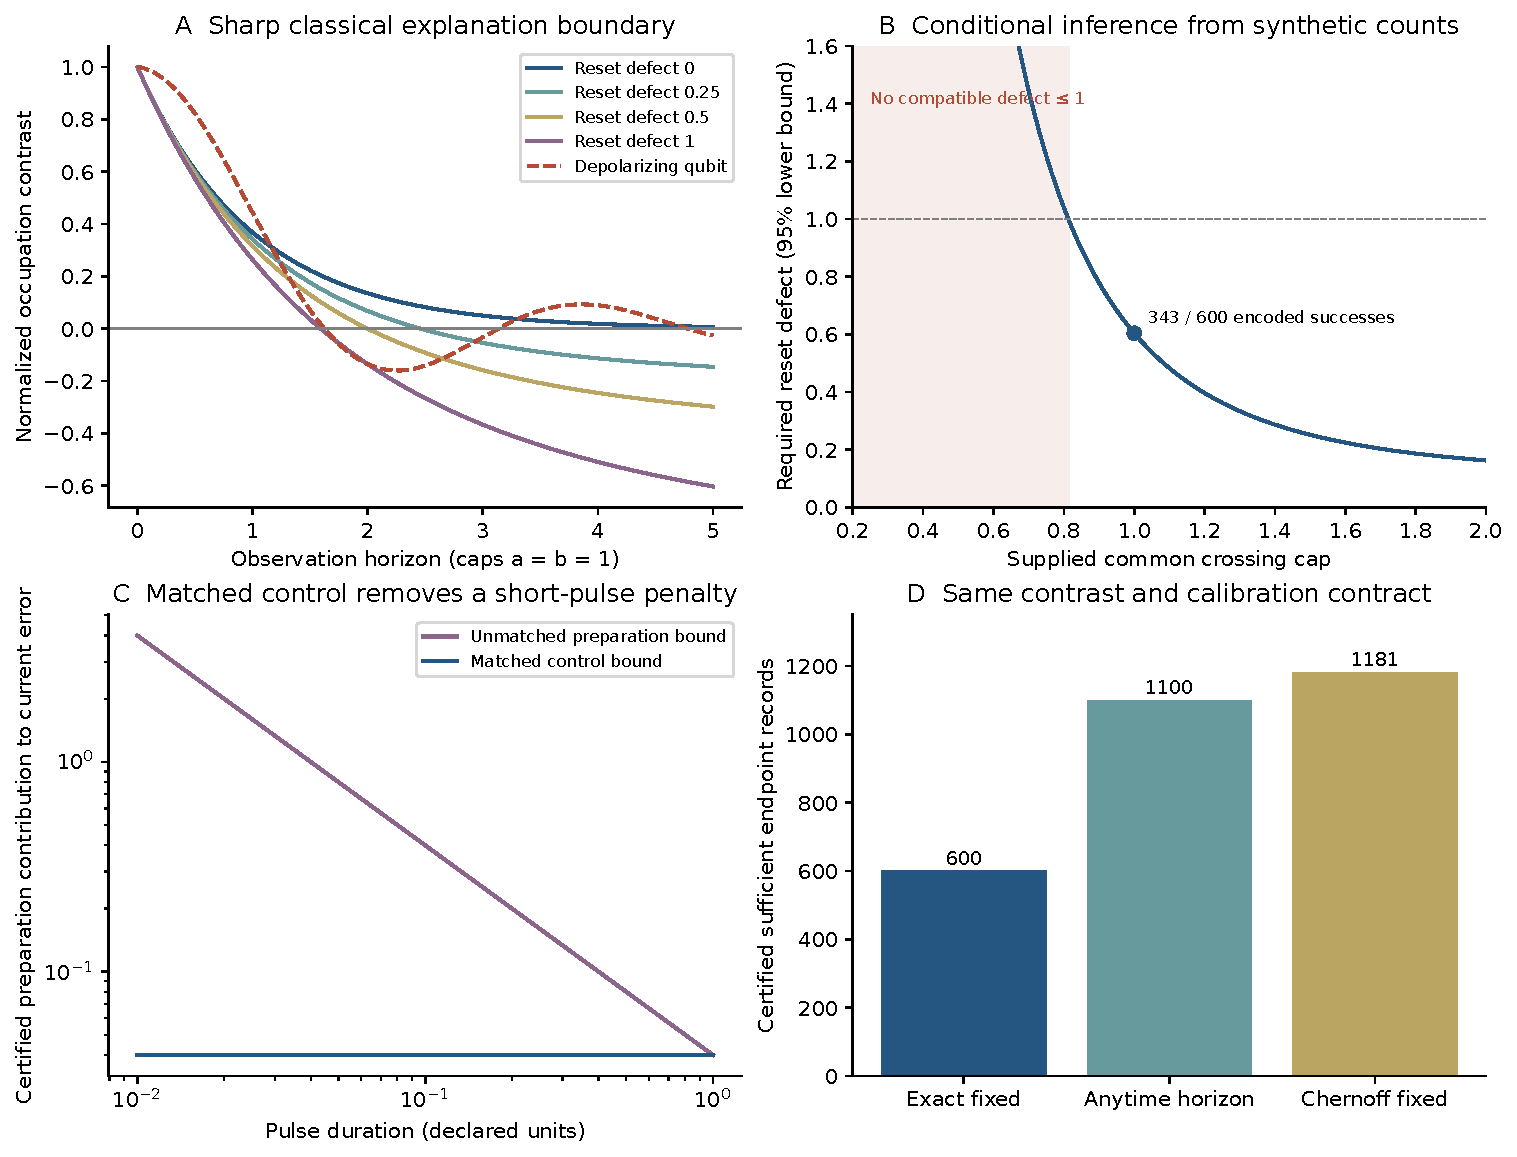
\includegraphics[width=\textwidth]{robust_results.pdf}
\caption{A: the sharp classical lower envelopes for several reset-defect caps,
with a depolarizing-qubit contrast as a model illustration. B: the required
reset defect from explicitly synthetic counts, conditional on the supplied
common crossing cap; values above one exclude that cap. C: preparation-error
contributions alone, for discrepancy $0.01$, channel rates $3,1$ and retention
$1/2$; matching the native control removes the $1/t$ penalty in this bound.
D: sufficient fixed and anytime record budgets for the same declared contrast,
calibration and 5\% error targets. The anytime bar is a guaranteed horizon,
not an expected stopping time. No panel contains physical measurements.}
\label{rr:overview}
\end{figure}

\section{A laboratory route that does not assume hidden reset purity}
The realization-size test asks a different question from reset-defect inversion.
Its target is whether a single homogeneous classical Markov description with
at most three states can explain the records. It needs two repeatable
preparation commands, one fixed binary readout, a common evolution setting,
and an independent clock. The preparations may be mixed and the readout may be
noisy. Hidden environmental and controller states that affect the dynamics
belong to the realization being bounded.

There are four equally randomized arms: each preparation is measured either
at the common reference time or after an independent uniform hold in $[0,T]$.
Use fresh trials and perform only the terminal measurement. The immediate and
delayed observations come from different trials; a baseline measurement must
not be inserted into the delayed evolution. Common latency is allowed when it
is shared by all arms and independent of the hold-time draw. Calibration must
bound changes between the arms, including preparation drift, detector drift,
and arm-dependent dynamics. A fixed detector's intrinsic noise is already
covered by the theorem.

The statistical chapter gives a complete four-arm encoding and a predeclared
record-count certificate. Its exact qubit alternative is a feasibility
prediction. The laboratory decision is a rejection of the calibrated
three-state description, not confirmation of a unique quantum mechanism.
A classical four-state control and a time-dependent three-state control test
how the interpretation fails when the relevant model assumptions change.
Time stamps should be retained for diagnostics, even when the stated decision
uses only the integrated statistic; no time-bin postselection belongs in that
decision rule.

\begin{figure}[htbp]
\centering
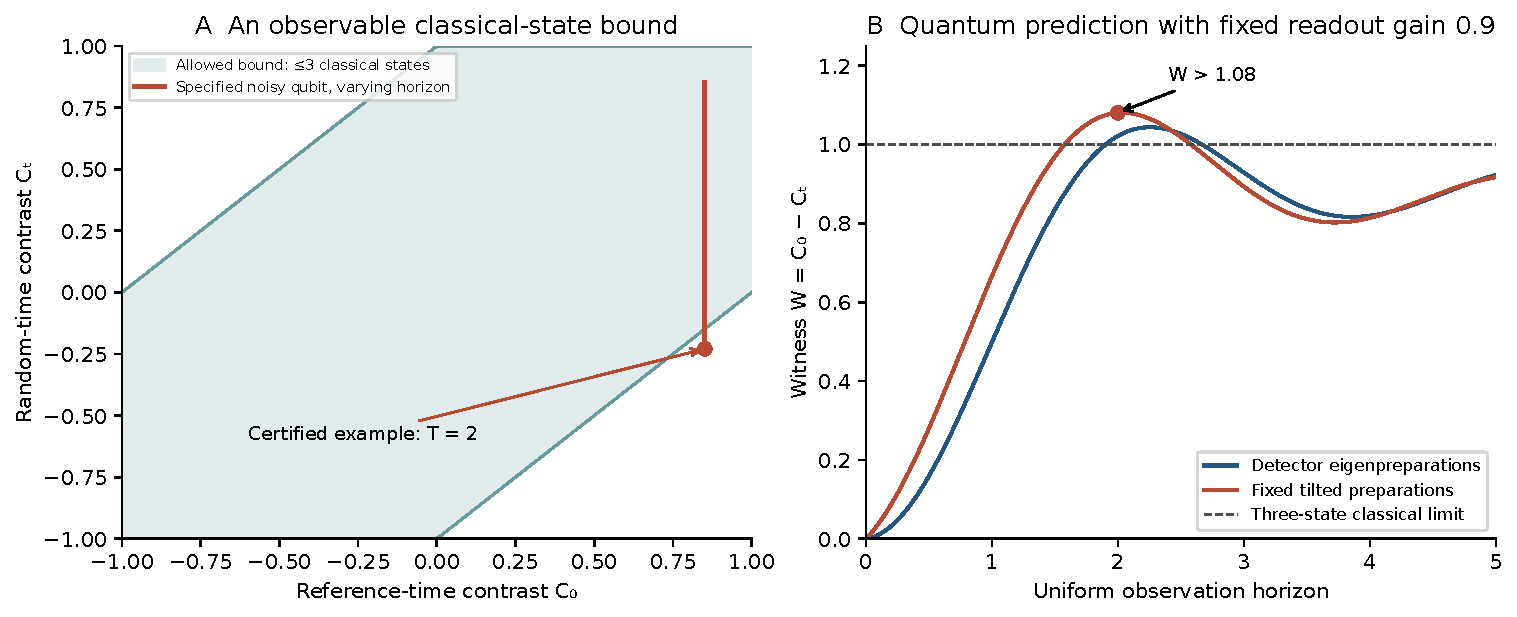
\includegraphics[width=\textwidth]{dimension_witness.pdf}
\caption{The integrated realization-size witness. The shaded strip contains
all common homogeneous classical models with at most three states, arbitrary
preparations and a fixed stochastic binary detector. The displayed qubit model
leaves this strip. The two quantum curves use different fixed preparation
pairs; neither is an experimental dataset or a claim of global optimality.}
\label{rr:dimension-figure}
\end{figure}

\section{From required records to a physical energy budget}
Record count, elapsed evolution, and energy answer different questions. Suppose
an independently calibrated apparatus contract supplies a gross preparation
and readout energy cap $E_0$ per trial and a gross holding-power cap $P_{\max}$.
Include any clock or controller expenditure covered by these caps, and write
$E_{\rm cal}$ for separate calibration and setup expenditure. A fixed $N$-record
uniform-hold protocol then satisfies the deterministic bound
\[
 E_{\rm total}\leq E_{\rm cal}+NE_0+NP_{\max}T.
\]
For the four-arm realization-size protocol, half the trials have no additional
hold and half have mean hold $T/2$. Therefore
\[
 \mathbb E E_{\rm total}
 \leq E_{\rm cal}+NE_0+NP_{\max}T/4.
\]
The expectation is not a pathwise guarantee. Common latency and other overhead
must be added if they are absent from $E_0$.

The 600-record protected-preparation example has expected additional evolution
675 in its declared time unit. The 6000-record four-arm example at $T=2$ has
expected additional evolution 3000. The latter purchases freedom from exact
hidden preparation assumptions at a measurable acquisition cost. Neither
number is a joule value until the apparatus caps and time unit are calibrated.
No thermodynamic minimum or energy advantage over other dimension witnesses
is implied by these conditional accounting formulas.

\chapter{What a compatible explanation must contain}
\label{rf:entry}

The access problem has a useful next form. Instead of asking only whether two
known mechanisms can be distinguished, ask what \emph{every} compatible
explanation must contain. The answer may be a minimum number of classical
states, a sufficiently large preparation resource, or sustained dissipation.
These are different physical quantities. Their inference requires different
experimental access, and they must not be collapsed into a universal scalar
``information cap.''

The following chapters establish complementary boundaries of this question.
A robust nonnegative-factorization argument turns one preparation and one
repeated channel into a finite-data hierarchy of classical state requirements.
Erlang observation clocks give another route: finite measured probabilities
certify a spectral obstruction without estimating exact hidden poles or
bounding unseen transition rates. This certificate works at lower coherence
than the explicit hierarchy example, but its sufficient record bound is much
larger.

A constructive converse prevents overinterpretation. Finite fresh-reset
prepare--wait--read records with continuous target probabilities can be approximated arbitrarily well by finite,
irreducible, detailed-balance classical models when hidden dimension, rates and
preparation resources are unrestricted. The construction retains timestamps
and accommodates adaptive choices between reset trials. It does not reproduce
arbitrary interventions within a persistent trajectory. Its explicit state and
preparation requirements explain why an unrestricted classical null cannot be
rejected uniformly from that restricted access.

Stationary pair observations impose additional structure. Reversible Markov
autocorrelations are nonnegative mixtures of decaying exponentials. A measured
departure from this class yields a quantitative preparation--housekeeping
requirement; stationary preparation strengthens it to a sustained entropy-rate
bound. Exact dual certificates turn uncertain finite observations into such
requirements without selecting a hidden network architecture.

\begin{center}
\begin{tabular}{p{0.29\textwidth}p{0.30\textwidth}p{0.30\textwidth}}
\toprule
Access and premise & Certified conclusion & Essential qualification\\
\midrule
Repeated common channel, fixed preparation and readout & Minimum classical state count & Hidden control and detector memory count as states\\
Finite reset records, unrestricted hidden resources & Constructive classical approximation & No nontrivial uniform test against the full null\\
Stationary noninvasive binary pairs & Entropy-production lower bound & Ordinary reversal and thermodynamic embedding required\\
Nonstationary pairs and a preparation budget & Preparation--housekeeping tradeoff & Reference mean cannot be inferred from transient mean\\
\bottomrule
\end{tabular}
\end{center}

This is an extension of the common access contract, not a replacement for
established system identification, positive realization or stochastic
thermodynamics. The useful contribution is an explicit chain from observations
to requirements on all members of a declared explanatory class, with exact
countermodels where that chain cannot proceed. Candidate historical novelty,
mathematical verification and laboratory validation remain separate questions.


\begin{figure}[ht]
\centering
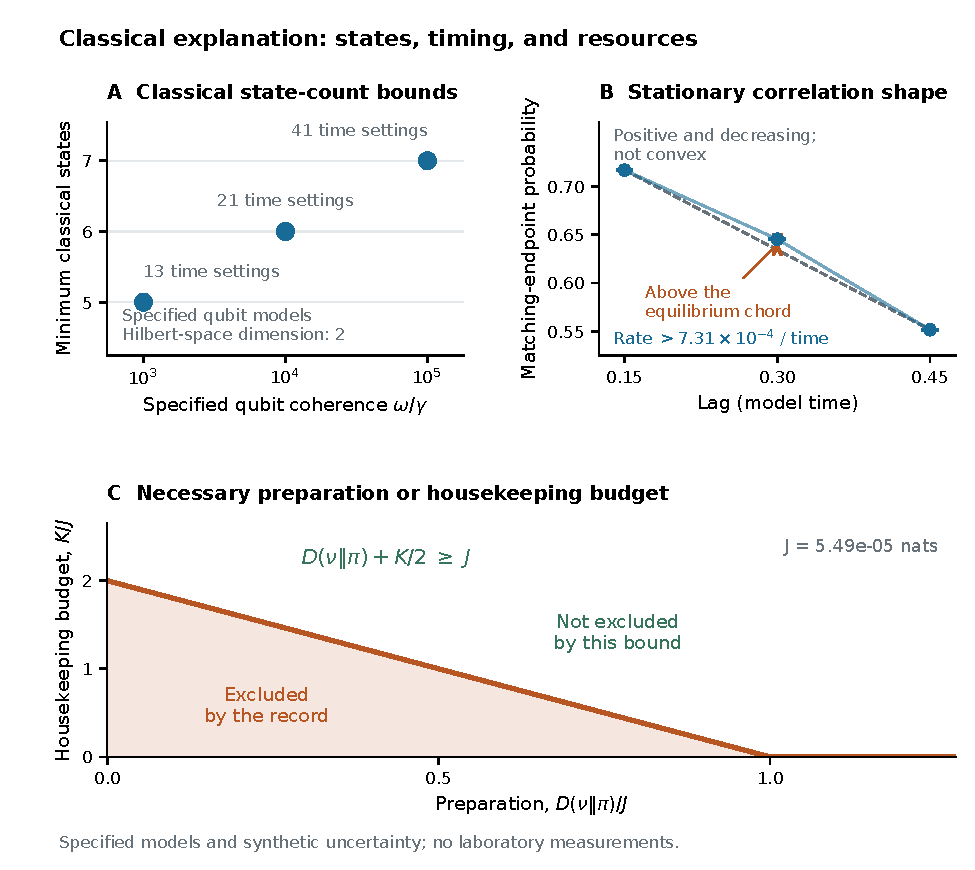
\includegraphics[width=\textwidth]{figures/realization_frontier.pdf}
\caption{Three types of requirements on a classical explanation.
(A) Specified finite-noise qubit examples force increasing classical state
counts under one repeated-channel contract; these points are not an optimized
coherence threshold. (B) The stationary ring example has positive decreasing
agreement probabilities but violates reversible convex decay. Error bars show
a synthetic uncertainty box. (C) A certified record separation $J$ excludes
preparation--housekeeping budgets below $D+K/2=J$. The region above the line
is merely not excluded by this bound; attainability is not asserted.
All panels are model-based and require their respective access assumptions.}
\label{rf:overview-figure}
\end{figure}

\chapter{A finite-record hierarchy of classical realization size}
\label{ch:finite-hierarchy}

The three-state occupation bound can exclude a small classical explanation,
but one scalar contrast cannot establish an unbounded hierarchy. Retaining
several observation times changes the mathematical object. A single prepared
state, a single binary detector, and a common repeated evolution produce a
matrix with a positive factorization through the hidden state space. This
chapter turns a robust obstruction to that factorization into a finite-record
experiment. The dimension is the total number of states of the proposed
classical Markov explanation, including any hidden controller or clock.

The foundations are established: positive realization and nonnegative-rank
bounds, Sperner's antichain theorem, and quantum dimension witnesses already
connect small quantum systems to larger classical realizations~\cite{rfGillis2020,rfShahandeh2024}. In particular,
the zero-noise sine matrix used below has appeared in prior work, including a
stronger six-factor lower bound for its seven-by-seven instance~\cite{rfHeinosaari2024}. The scoped
addition developed here is a nonzero-noise certificate, its realization through
one repeated channel and finitely many observation times, and an exactly checked
finite-record statistical protocol. Historical priority of that combination is
not established by this internal derivation.

\section{The operational model}
Let $P$ be any $n\times n$ stochastic matrix, $\alpha$ a probability row, and
$f\in[0,1]^n$ a fixed stochastic binary readout. Independent reset experiments
observe a binary outcome after $k$ applications of the same channel, with mean
\begin{equation}
 p_k=\alpha P^k f.                                      \label{eq:hier-pk}
\end{equation}
A continuous-time homogeneous chain is included by $P=e^{\Delta Q}$. The
result also covers repeated stochastic interventions, and independent,
identically distributed nonnegative timing increments with
$P=\mathbb E[e^{QZ}]$. It does not require a generator, stationarity, reversibility,
known rates, pure preparations, or a noiseless detector.

Fix $N\ge2$ and measure $p_1,\ldots,p_{2N-1}$. Form the matrix
\begin{equation}
 M_{ij}=p_{N+i-j},\qquad 0\le i,j<N.
                                                        \label{eq:hier-matrix}
\end{equation}
It factors as $M=AB$, where $A_i=\alpha P^i$ and $B_j=P^{N-j}f$.
Every row of $A$ is a probability vector and every entry of $B$ lies in $[0,1]$.
The reversal of the column index is only a permutation of a finite Hankel
matrix. There are $2N-1$ distinct measurement settings, not $N^2$ distinct
experiments. The diagonal entries all equal $p_N$.

\section{A robust antichain certificate}
\begin{theorem}[Finite-noise positive-factorization obstruction]
\label{thm:robust-antichain}
Suppose an $N\times N$ matrix admits $M=AB$ with $n$ columns in $A$,
probability rows in $A$, and $0\le B_{kj}\le1$. If
\begin{equation}
 M_{ii}\le\epsilon,\qquad M_{ij}\ge\beta\quad(i\ne j),
 \qquad
 \beta>\tau+(1-\tau)\frac{\epsilon}{\tau}
                                                        \label{eq:hier-margin}
\end{equation}
for some $0<\tau<1$, then
\begin{equation}
 N\le {n\choose\lfloor n/2\rfloor}.                     \label{eq:hier-sperner}
\end{equation}
For $0<\epsilon<1$, minimizing the right side of
\eqref{eq:hier-margin} over $\tau$ gives the sufficient condition
$\beta>2\sqrt\epsilon-\epsilon$. For $\epsilon=0$, any $\beta>0$
suffices.
\end{theorem}
\begin{proof}
Write $a_i$ for row $i$ of $A$, and define
$S_i=\{k:B_{ki}<\tau\}$. The diagonal bound gives
$a_i(S_i^c)\le\epsilon/\tau$. If $S_i\subseteq S_j$, then
\[
 M_{ij}\le\tau a_i(S_j)+a_i(S_j^c)
 \le\tau+(1-\tau)\epsilon/\tau,
\]
contradicting \eqref{eq:hier-margin}. Thus the $N$ subsets $S_i$ are pairwise
incomparable. Sperner's theorem bounds their number by the largest binomial
coefficient. The minimum of $\tau+\epsilon/\tau-\epsilon$ is obtained at
$\tau=\sqrt\epsilon$. When $\epsilon=0$, take $S_i=\{k:B_{ki}=0\}$.
The diagonal condition puts all of $a_i$ on $S_i$, and inclusion
$S_i\subseteq S_j$ would give $M_{ij}=0$.
\end{proof}

This certificate supplies a sufficient lower bound, not the nonnegative rank
itself and not the minimum dimension of a positive dynamical realization.
Those quantities need not coincide. The antichain cardinality bound is sharp
for unrestricted stochastic factors: use all subsets of size $\lfloor n/2\rfloor$,
let $a_i$ be uniform on subset $S_i$, and let $B_{kj}$ indicate $k\notin S_j$.
The diagonal is zero and every off-diagonal entry is positive. This construction
does not establish sharpness for a single-channel Hankel matrix.

\begin{corollary}[One-channel finite-time dimension hierarchy]
\label{cor:hierarchy}
If the records \eqref{eq:hier-pk} satisfy $p_N\le\epsilon$ and
$p_k\ge\beta$ for every $1\le k\le2N-1$, $k\ne N$, with
\eqref{eq:hier-margin}, their classical homogeneous Markov realization requires
at least
\[
 d_*(N)=\min\left\{n:{n\choose\lfloor n/2\rfloor}\ge N\right\}
\]
hidden states. In particular $N=7,11,21,71$ require respectively at least
$5,6,7,9$ states.
\end{corollary}

\section{An explicit qubit family}
Prepare a qubit in $|0\rangle$, use a fixed $|1\rangle$ detector, and evolve
with
\[
 \mathcal L(\rho)=-i\frac{\omega}{2}[X,\rho]
 +\gamma\bigl(\operatorname{tr}(\rho)I/2-\rho\bigr).
\]
Set $r=\omega/\gamma$ and $\Delta=2\pi/(N\omega)$. The measured means are
\begin{equation}
 p_k=\frac{1-e^{-2\pi k/(rN)}\cos(2\pi k/N)}2.
                                                        \label{eq:hier-qubit}
\end{equation}
For $N\ge4$, their diagonal value is
$\epsilon_r=(1-e^{-2\pi/r})/2$, and all the off-diagonal values are at least
$\sin^2(\pi/N)$. If the cosine is nonnegative, damping increases the probability
above its unitary value; if it is negative, the probability remains at least
$1/2\ge\sin^2(\pi/N)$. It follows that any fixed desired finite state lower
bound can be reached at a sufficiently large, but finite, coherence ratio.
This is a hierarchy of finite-resource experiments, not one finite experiment
that excludes all finite classical models.

The sufficient coherence condition can be written
\begin{equation}
 \epsilon_r < \bigl(1-\cos(\pi/N)\bigr)^2.
                                                        \label{eq:hier-coherence}
\end{equation}
For large $N$ its right side is of order $N^{-4}$. Since $N$ itself grows
roughly exponentially in the desired state count, this certificate is not an
efficient route to arbitrarily large dimension exclusions. Its transparent
finite-noise guarantee is the benefit; efficiency and optimality remain
separate questions. No relation between $r$ and thermodynamic energy is assumed.

The exact-arithmetic implementation gives the following demonstrations:
\begin{center}
\begin{tabular}{rrrr}
$N$ & observation settings & $\omega/\gamma$ & certified states\\
\hline
7 & 13 & $10^3$ & at least 5\\
11 & 21 & $10^4$ & at least 6\\
21 & 41 & $10^5$ & at least 7
\end{tabular}
\end{center}
They are calculated qubit probabilities. None is a laboratory observation.

\section{A finite-record test without a multiplicity penalty on type I error}
Choose a forbidden rectangular probability region
$p_N\le\epsilon_0$ and $p_k\ge\beta_0$ for $k\ne N$, satisfying
\eqref{eq:hier-margin}. For each setting collect an independent fixed number
$n_k$ of reset records, and let $S_k$ be the success count. Reject the proposed
classical dimension only when
\begin{equation}
 S_N\le c_N\quad\hbox{and}\quad S_k\ge c_k\quad(k\ne N).
                                                        \label{eq:hier-test}
\end{equation}
Calibrate each individual tail at its boundary to be at most $\alpha$.
Every model in the excluded classical class violates at least one of the
probability constraints. The probability of passing every count criterion is
therefore at most the rejection probability for that one violated constraint,
which is at most $\alpha$. A Bonferroni division of $\alpha$ among settings is
unnecessary. This is an intersection--union test, an established statistical
construction. For a specified alternative, the probability of failing any
criterion is bounded by the sum of its individual miss probabilities.

Here is a fully specified example. Set $N=7$, $r=1000$,
$\epsilon_0=3/500$, $\beta_0=3/20$, and $\tau=2/25$.
The classical comparison bound is $149/1000<\beta_0$.
Use the following counts and acceptance conditions:
\begin{center}
\begin{tabular}{rrrr}
Step $k$ & Records $n_k$ & Critical count $c_k$ & Requirement\\
\hline
1 &1900&313&$S_1\ge313$\\
2--5 &100 each&22&$S_k\ge22$\\
6 &1800&297&$S_6\ge297$\\
7 &10300&48&$S_7\le48$\\
8 &1800&297&$S_8\ge297$\\
9--12 &100 each&22&$S_k\ge22$\\
13 &1700&282&$S_{13}\ge282$
\end{tabular}
\end{center}
At $k=7$ require $S_7\le48$; elsewhere require $S_k\ge c_k$.
The total is $18\,300$ binary records and $126\,900$ channel applications.
The exact certificates imply
\begin{equation}
 \Pr_{n\le4}(\text{reject})<0.049048,
 \qquad
 \Pr_{\text{specified qubit}}(\text{do not reject})<0.015708.
                                                        \label{eq:hier-errors}
\end{equation}
The elapsed evolution time is $126900\Delta$, excluding preparation,
reset, readout, and controller overhead. An energy cost cannot be inferred
from this operation count without a physical implementation and calibration.
The record count is a checked sufficient design; no global optimality is claimed.

The probability intervals are certified with rational Machin-formula bounds
on $\pi$ and Taylor remainders. A binomial tail is bounded using its boundary
mass and a geometric series whose ratio bounds all successive masses in the
tail. All reported error comparisons use integer or rational arithmetic.
Floating-point quantiles only propose critical counts; they do not certify them.

\section{Calibration, timing and failure cases}
If recorded means differ from a common-model mean by at most a known absolute
amount $\delta$, use null boundaries $\epsilon_0-\delta$ and
$\beta_0+\delta$ in the two count tails. For a predicted alternative with the
same uncertainty, its adverse bounds become $p_N+\delta$ and
$p_k-\delta$. Calibration failure probability, if any, is added separately.
The supplied routine implements this conservative extension, although the
numerical design \eqref{eq:hier-errors} uses $\delta=0$.

No hidden-state preparation purity or rate bound is required. What must be
stable is the preparation distribution, repeated channel, and readout across
settings. A one-state device with a readout chosen according to $k$ can fake
any sequence $p_k$; a time-dependent or history-dependent classical process
can also invalidate the factorization. Controller state must either be reset
or included in the count. Arbitrary independent jitter at each total wait time
need not preserve the additive grid when hidden rates are unbounded; a common
random preparation latency, or independent identical increments composing each
step, does preserve the repeated-channel model. General timing uncertainty
requires a separate calibrated record-probability bound.

For context, an $N$-state deterministic discrete cycle with detector values
$\sin^2(\pi j/N)$ reproduces the ideal unitary sequence exactly. Thus the
certificate demonstrably excludes small classical models while allowing a
larger classical explanation. It is neither a proof of nonclassicality against
all models nor a new universal physical law.

\chapter{Finite random-clock certificates for classical realization size}
\label{ch:finite-erlang}

An observed damped oscillation can require a large classical realization even
when a qubit produces it. This fact and the relevant spectral obstruction are
established \cite{rrWolf2009}. The practical difficulty is different: finite,
noisy observations do not determine an exact pole. We therefore measure a finite
list of bounded probabilities whose distance from every small classical model
can be certified directly. The resulting tolerance is conservative; at high
dimension it is much too small for a practical experiment.

\section{The operational contract}
Let $Q$ be a conservative, homogeneous generator with at most $n$ hidden states,
$\rho$ an unknown but fixed initial probability row, and $f\in[0,1]^n$ an unknown
but fixed binary response vector. The detector may be probabilistic. Neither
stationarity, reversibility nor a bound on the exit rates is assumed. Each trial
starts from $\rho$ and measures $f$ at a time chosen independently of the physical
process. The clock does not change the generator, preparation or detector.

Fix a rate $s>0$. For $k\geq1$, choose an Erlang clock $T_k$ with shape $k$ and
rate $s$; set $T_0=0$. Resolvent integration gives
\begin{equation}
 m_k=\mathbb E[\rho e^{QT_k}f]=\rho R^k f,
 \qquad R=s(sI-Q)^{-1}.
 \label{eq:erlang-resolvent}
\end{equation}
The matrix $R$ is stochastic. Thus independently randomized observation times
convert a continuous-time record into finitely many powers of one stochastic
matrix, without estimating derivatives or the hidden exit rates.

The comparison signal is the $+Z$ occupation probability of a qubit prepared
in $+Z$, rotating under $\omega X/2$ with isotropic depolarization rate $\gamma$:
\begin{equation}
 p_*(t)=\frac{1+e^{-\gamma t}\cos(\omega t)}2,
 \qquad
 m_k^*=\frac{1+\operatorname{Re}\mu^k}2,
 \qquad \mu=\frac{s}{s+\gamma-i\omega}=u+iv.
 \label{eq:erlang-qubit}
\end{equation}
Here $\omega,s>0$, $\gamma\geq0$, and $v>0$. Rational rates give rational
probabilities $m_k^*$, even though the observation times are continuous.

\section{A finite robustness theorem}
The established generator spectral bound is
\begin{equation}
 |\operatorname{Im}\lambda|
 \leq-\operatorname{Re}\lambda\cot(\pi/n).
 \label{eq:generator-sector-rf}
\end{equation}
Writing $t_n=\tan(\pi/n)$ shows that every eigenvalue $z$ of $R$ lies in the lens
\begin{equation}
 |z|^2-\operatorname{Re}z+t_n|\operatorname{Im}z|\leq0.
 \label{eq:resolvent-lens}
\end{equation}
In particular, for any certified $0<t_0\leq t_n$, the lens is contained
in both reflected disks with centers $1/2\pm it_0/2$ and radius
$\sqrt{1+t_0^2}/2$.

For the sharper bound it is useful to normalize the characteristic polynomial.
Define
\[
 \nu=\frac{1-\mu}{1+\mu}=a-ib,\qquad b>0,\qquad
 K=\sqrt{1+(1+u)^2/v^2},\qquad q=\lfloor(n-1)/2\rfloor.
\]
If $\gamma/\omega<t_0$, then $\nu$ is outside the upper-centered bounding disk.
Choose
\[
 0<d\leq\min\left\{b,
 \left|\nu-\left(\tfrac12+\tfrac{it_0}{2}\right)\right|
 -\frac{\sqrt{1+t_0^2}}2\right\},\qquad
 r_0=\frac{v}{|1+\mu|},\qquad
 h=\frac{|1+\mu|^2}{4}d(2b-d).
\]
Notice that $h\leq r_0^2$.

\begin{theorem}[Finite Erlang exclusion]
\label{thm:finite-erlang}
Under the preceding assumptions, every classical model with at most $n\geq3$
states satisfies
\begin{equation}
 \max_{0\leq k\leq n+1}|m_k-m_k^*|
 \geq\Delta_n,
 \qquad
 \Delta_n=\frac{|1-\mu|\,r_0^{n-1-2q}h^q}{4K}>0.
 \label{eq:finite-erlang-gap}
\end{equation}
Only $n+2$ observation settings enter this inequality. No fitted pole, exact
rank determination, spectral visibility assumption, or exit-rate bound is used.
\end{theorem}

\begin{proof}
Pad a smaller model by unreachable absorbing states. Let $P$ be the real monic
characteristic polynomial of its $n\times n$ stochastic resolvent $R$, and let
$C$ be the sum of the absolute values of its coefficients. The resolvent roots
have positive real parts. Each real-linear and conjugate-quadratic factor has
alternating coefficients, and products preserve those signs. Hence
$C=|P(-1)|$. Also $P(1)=0$ and $P(R)=0$.

If the maximum moment error is $\varepsilon$, Cayley--Hamilton applied at shifts
zero and one gives
\[
 |\operatorname{Re}P(\mu)|\leq2\varepsilon C,
 \qquad
 |\operatorname{Re}(\mu P(\mu))|\leq2\varepsilon C.
\]
The constant half of~\eqref{eq:erlang-qubit} cancels because $P(1)=0$.
Writing $P(\mu)=A+iB$ yields
$|B|\leq2\varepsilon C(1+u)/v$ and therefore
$|P(\mu)|/C\leq2\varepsilon K$.

For any root $z=s/(s-\lambda)$, put
\[
 w=\frac{1-z}{1+z}=1-\frac{2s}{2s-\lambda}.
\]
The lens~\eqref{eq:resolvent-lens} is invariant under $z\mapsto1-z$, so $w$ lies
in the same lens. Direct algebra gives
\[
 \frac{|\mu-z|}{|1+z|}=\frac{|1+\mu|}{2}|\nu-w|.
\]
A real root therefore contributes at least $r_0$. For a conjugate pair write
$y=|\operatorname{Im}w|$. If $y\geq b-d$, the near factor is at least $d$ and
the far factor at least $b+y\geq2b-d$. If $y\leq b-d$, their product is at least
$(b-y)(b+y)\geq d(2b-d)$. Thus each normalized conjugate pair contributes at
least $h$. One root $z=1$ contributes $|1-\mu|/2$. Because $h\leq r_0^2$,
the most conservative product uses the maximum number $q$ of pairs:
\[
 \frac{|P(\mu)|}{|P(-1)|}
 \geq\frac{|1-\mu|}{2}r_0^{n-1-2q}h^q.
\]
Combining the two inequalities proves the result. Defective matrices cause no
problem because the argument uses the characteristic polynomial, not an
eigenvector decomposition.
\end{proof}

The distance calculation is entirely reproducible with rational interval
arithmetic. If $F=|\nu-c|^2-r^2>0$, then
\[
 |\nu-c|-r=\frac{F}{|\nu-c|+r}.
\]
Rational upper bounds on the denominator give a lower bound on the distance.
The implementation obtains $t_0$ from Machin's formula for $\pi$, alternating
arctangent bounds and $\tan x\geq x+x^3/3$; for $n=4$ it uses $t_0=1$ exactly.
Integer square roots give directed dyadic bounds for the remaining radicals.

\section{Finite duration, calibration and sampling}
The ideal Erlang clock is unbounded. A laboratory implementation can return an
artificial zero when $T_k>L$, without waiting beyond $L$. Its moment changes by
at most
\begin{equation}
 \tau_k(L)=\Pr(T_k>L)
 =e^{-sL}\sum_{j=0}^{k-1}\frac{(sL)^j}{j!}.
 \label{eq:erlang-tail}
\end{equation}
This tail is bounded above by replacing $e^{-sL}$ with the reciprocal of a
positive partial sum for $e^{sL}$. No hidden dynamical rate appears in the bound.

Let $\widehat m_k$ be sample means from $N$ independent trials per setting,
$r_N$ a simultaneous confidence radius, $b$ a calibrated probability error, and
$\tau\geq\max_k\tau_k(L)$. A valid rejection rule is
\begin{equation}
 \max_k|\widehat m_k-m_k^*|+r_N+b+\tau<\Delta_n.
 \label{eq:erlang-statistical-test}
\end{equation}
Hoeffding and a union bound give confidence at least
$1-2(n+2)e^{-2Nr_N^2}$. The same data cannot first select an unrestricted target
and then use a confidence guarantee proved only for a predeclared target.

The supplied design takes $r_N=\Delta_n/4$ and $\tau\leq\Delta_n/8$. With $b=0$,
both false rejection of the classical class and missed detection of the nominal
qubit target are at most the declared $\alpha$. Under the target, the confidence
event gives total distance at most $2r_N+2\tau<\Delta_n$. For an additional
calibration radius, the corresponding power guarantee requires
$2r_N+2\tau+2b<\Delta_n$.

\section{What the certificate achieves, and its cost}
For $\gamma=1/10$, $\omega=2$ and $s=13/10$, exact arithmetic certifies
\[
 n=4:\qquad\Delta_4>0.0016816962795.
\]
There are six clock settings. A fully bounded design with duration at most
$320/13$ and $\alpha=0.05$ uses a conservative total of $135{,}780{,}096$
records. This large count is a limitation of the current sufficient bound, not
a claim of practical superiority. The result closes a qualitative gap: a
strictly positive finite-data exclusion exists without assuming an exact pole
or bounding the rates of invisible modes.

\begin{center}
\begin{tabular}{r r l}
Excluded state count $n$ & Clock settings & Certified uniform gap\\\hline
4 & 6 & $1.6816962795\times10^{-3}$\\
5 & 7 & $3.2905352735\times10^{-4}$\\
6 & 8 & $8.2677897333\times10^{-5}$\\
8 & 10 & $2.7407114770\times10^{-6}$\\
16 & 18 & $1.5863939618\times10^{-13}$\\
62 & 64 & $1.1657896420\times10^{-117}$
\end{tabular}
\end{center}
All entries concern the same damped qubit; the Erlang rate is chosen separately
for each declared $n$ and recorded in the reproducibility data. The last entries
are constructive mathematical bounds, not recommended experimental plans.

A four-state directed cycle of rate $2$, with fixed response probabilities
$(1,1/2,0,1/2)$, exactly produces
$(1+e^{-2t}\cos2t)/2$. The certificate correctly stops separating at
$\gamma=\omega$ for $n=4$. Larger cyclic classical realizations exist for every
strictly damped sinusoid when sufficiently many states are allowed. Thus the
witness bounds classical realization size; it does not exclude every classical
explanation or convert a state count into a thermodynamic energy cost.

The spectral obstruction, resolvent representation and linear recurrence
machinery are established ingredients. The contribution investigated here is
the explicit finite-setting, bounded-duration robustness certificate and its
checkable error accounting. Historical priority remains open. Improving its
sample complexity is a separate research problem; the finite probability-table
witness elsewhere in this reference supplies a substantially stronger practical
comparison in its effective regime.

\chapter{What finite reset experiments cannot exclude}
\label{rf:limits}

An observable that excludes a three-state classical model does not exclude
classical models with unrestricted hidden resources. This distinction survives
precise timestamps, adaptive scheduling, and arbitrarily accurate finite
records. This chapter constructs the alternative models explicitly. It also
shows that a transient coherent-looking signal need not identify nonzero
\emph{stationary} dissipation: a classical model satisfying detailed balance
can approximate the same records by starting far from equilibrium.

The approximation machinery is established. In particular, the Poisson
operator used below is the Sz\'asz--Mirakjan operator, introduced in the
classical approximation literature\cite{rfSzasz1950}. The role of the result
here is to locate the operational boundary of inference and count the hidden
resources needed by a sufficient countermodel. It is not a claim of a new
universal approximation principle.

\section{The access contract}

Let $a\in\{1,\ldots,m\}$ label finitely many preparations, and let
$p_a(t)\in[0,1]$ be the probability of a fixed binary detector outcome after
waiting for time $t$. Each record begins with a fresh preparation. Its arm and
waiting time may depend on earlier records, but are chosen independently of
the subsequent hidden noise in that record. The apparatus retains the arm,
waiting time, and outcome. The initial theorem concerns $t\in[0,T]$.

The classical comparison class has one common homogeneous finite Markov
generator, one fixed detector, and a distribution for each preparation. All
hidden clock and preparation-label states count toward its dimension. No
intermediate measurement or control during the wait is included. The theorem
does not reconstruct joint laws of repeated nondestructive measurements on a
single persistent system, nor does it match independently measured energy or
preparation-resource observables.

\section{A finite homogeneous classical realization}

\begin{theorem}[Explicit finite-window approximation]
\label{rf:poisson-realization}
Suppose all $p_a:[0,T]\to[0,1]$ have Lipschitz constant at most $L>0$.
For every $r>0$, there is a common homogeneous finite Markov generator with
deterministic binary readout, at most
\[
 n=2m(\lceil rT\rceil+1)
\]
states, and peak exit rate at most $r$, whose output probabilities satisfy
\begin{equation}
 \sup_{a,\,0\le t\le T}|q_a(t)-p_a(t)|
 \le L\sqrt{T/r}.
 \label{rf:lipschitz-realization}
\end{equation}
Thus $r=L^2T/\varepsilon^2$ is sufficient for error $\varepsilon$.
\end{theorem}

\begin{proof}
Set $K=\lceil rT\rceil$ and $f_a(k)=p_a(\min(k/r,T))$. A pure-birth clock
$k=0,\ldots,K$ starts at zero, jumps forward at rate $r$, and stays at $K$
thereafter. Introduce states $(a,k,y)$ with $y\in\{0,1\}$ and detector value
$y$. On moving to phase $k+1$, choose the new bit according to
$\operatorname{Bernoulli}(f_a(k+1))$. Initially choose the bit according to
$\operatorname{Bernoulli}(f_a(0))$. This is a homogeneous Markov model; the
label $a$ selects an initial component of its common generator.

If $N_{rt}$ is Poisson with mean $rt$, its detector probability is
\[
 q_a(t)=\mathbb E\,p_a\bigl(\min(N_{rt}/r,T)\bigr).
\]
Projection onto $[0,T]$ cannot increase distance from $t$. The Lipschitz
bound and Cauchy--Schwarz therefore give
\[
 |q_a(t)-p_a(t)|\le L\mathbb E|N_{rt}/r-t|
 \le L\sqrt{\operatorname{Var}(N_{rt}/r)}
 =L\sqrt{t/r}.
\]
The claimed state and rate bounds follow directly from the construction.
\end{proof}

Zero-probability bit states may be deleted. Uniform error $\eta$ in tabulating
the phase probabilities adds at most $\eta$ to the output bound. Preparations
with $p_a(0)=0$ or $1$ remain supported entirely on the appropriate detector
region: the construction does not rely on disguising an error at time zero.

\begin{proposition}[Smooth approximation and finite truncation]
\label{rf:smooth-realization}
Suppose $p_a:[0,\infty)\to[0,1]$ is twice differentiable and
$|p_a''(t)|\le M$ for every $a,t$. A clock frozen at phase $K$, tabulated using
$f_a(k)=p_a(k/r)$, satisfies
\begin{equation}
 \sup_{a,\,0\le t\le T}|q_a(t)-p_a(t)|
 \le \frac{MT}{2r}+\Pr\{\operatorname{Poisson}(rT)\ge K\}.
 \label{rf:smooth-clock-bound}
\end{equation}
\end{proposition}

\begin{proof}
For the untruncated clock, Taylor's linear term averages to zero because
$\mathbb E(N_{rt}/r)=t$. The second-order remainder is at most
$M\mathbb E(N_{rt}/r-t)^2/2=Mt/(2r)$. Freezing changes a bounded detector
mean by at most the probability of reaching the truncation region. Poisson
tail monotonicity in $t$ gives the stated bound.
\end{proof}

The global derivative assumption matters: the untruncated clock can query
times beyond $T$. For rational $\mu=rT$, an exact finite tail certificate is
\begin{equation}
 \Pr\{N\ge K\}\le
 \min_{0\le s\le K}\frac{\mu^s}{(K)_s},
 \qquad N\sim\operatorname{Poisson}(\mu),
 \label{rf:factorial-tail}
\end{equation}
where $(K)_s=K(K-1)\cdots(K-s+1)$ and the $s=0$ term is one.
It follows from the factorial moment $\mathbb E(N)_s=\mu^s$.
For very large state bounds the implementation also uses the simpler Cantelli
certificate
\[
 \Pr\{N\ge K\}\le \frac{\mu}{\mu+(K-\mu)^2},\qquad K>\mu.
\]
These are sufficient bounds, without an optimality claim.

For a finite-dimensional Lindblad generator $\mathcal L$ and fixed binary
effect $E$, all preparations satisfy usable global bounds
\[
 L=\|\mathcal L^*(E)\|_\infty,\qquad
 M=\|(\mathcal L^*)^2(E)\|_\infty,
\]
as chosen Lipschitz and curvature constants. Indeed the derivatives are expectations of these Hermitian
operators in the evolved density matrix. Thus every finite set of
preparations of a finite-dimensional Lindblad semigroup fits the construction.
The constructed classical clock rates need not equal the Lindblad damping
rates and are not inferred physical parameters.

\section{A detailed-balance countermodel with a preparation cost}

\begin{theorem}[Reversible realization]
\label{rf:reversible-realization}
Replace the clock's forward rate $r$ by forward and backward rates $r,d>0$,
with reflecting endpoints. Keep the destination-phase bit sampling used
above. The resulting classical model satisfies detailed balance and has zero
stationary entropy production. Its output probabilities differ from those of
the one-way clock by at most
\begin{equation}
 1-e^{-dT}\le dT
 \label{rf:backward-coupling}
\end{equation}
uniformly on $[0,T]$. Let $R=r/d$ and $Z=\sum_{k=0}^{K}R^k$. Relative to the
stationary law with equally weighted preparation components, the prescribed
initial state has relative entropy
\begin{equation}
 D(\nu_a\Vert\pi)=\log(mZ).
 \label{rf:preparation-cost}
\end{equation}
\end{theorem}

\begin{proof}
The phase chain has stationary weights $R^k/Z$. Write
$b_a(k,y)=f_a(k)^y[1-f_a(k)]^{1-y}$, with its usual Bernoulli interpretation
at endpoints. The lifted stationary law is
\[
 \pi(a,k,y)=\frac{R^k}{mZ}b_a(k,y).
\]
For neighboring phases $k,\ell$, the jump rate is $q_{k\ell}b_a(\ell,z)$.
The two stationary edge flows agree because
\[
 R^k b_a(k,y)q_{k\ell}b_a(\ell,z)
 =R^\ell b_a(\ell,z)q_{\ell k}b_a(k,y).
\]
Delete zero-weight bit states. Every retained state has positive stationary
weight within its component. Couple the forward jumps and sampled bits with
the one-way process until a backward jump occurs. The backward-jump counting
process is dominated by a rate-$d$ Poisson process, which proves
\eqref{rf:backward-coupling}. Finally,
$\nu_a(a,0,y)=b_a(0,y)$, so its likelihood ratio relative to $\pi$ equals
$mZ$ on its support. This proves \eqref{rf:preparation-cost}.
\end{proof}

If a single irreducible generator is required, add
$c(\mathbf 1\pi-I)$ for any $c>0$ on the retained states. This introduces
rare resets to $\pi$, connects all components, and preserves detailed balance.
A reset-event coupling adds at most $cT$ to the approximation error. Thus
arbitrarily accurate reversible approximations do not depend on reducibility
or absorbing states.

Zero \emph{stationary} entropy production does not imply zero transient
entropy production, zero reset cost, or free hardware. For an isothermal
detailed-balance realization at temperature $\Theta$,
$k_{\mathrm B}\Theta\log(mZ)$ is the nonequilibrium free-energy difference
from the specified equilibrium reference. It provides the corresponding
preparation-work lower bound from equilibrium when suitable reversible
controls are available. If the component label is conditioned on, the
within-component divergence is $\log Z$. The result assigns no universal
preparation charge to an arbitrary initial state supplied without a preparation
model. It does expose where a reversible classical imitation stores its
resource: highly nonequilibrium initialization of a large hidden clock.

\section{Retained timestamps, adaptive experiments, and a testing limit}

\begin{theorem}[Transcript approximation]
\label{rf:transcript-approximation}
Suppose the one-record output probabilities of the target and classical model
differ by at most $\varepsilon$ for every allowed preparation and waiting time.
For any fresh-reset protocol using at most $N$ records, including adaptive
choices and bounded stopping, their complete retained transcript laws obey
\begin{equation}
 \operatorname{TV}(P,Q)\le 1-(1-\varepsilon)^N\le N\varepsilon.
 \label{rf:transcript-tv}
\end{equation}
\end{theorem}

\begin{proof}
While the histories agree, share the random choices of next preparation and
waiting time. Conditional on those choices, couple the two Bernoulli outputs
maximally. The mismatch probability is at most $\varepsilon$ at every step.
Thus all records agree with probability at least $(1-\varepsilon)^N$.
The coupling inequality proves the result, including the retained timestamps.
\end{proof}

\begin{corollary}[No uniform quantum test against an unrestricted reset class]
\label{rf:closure-nogo}
Let $\mathcal C$ include every finite detailed-balance classical Markov model
with the access contract above and no bound on hidden dimension, rates, or
preparation resources. For a finite-record test $0\le\phi\le1$, suppose
\[
 \sup_{Q\in\mathcal C}\mathbb E_Q\phi\le\alpha.
\]
Then every smooth quantum prepare--wait--read law $P$ in the same contract
satisfies $\mathbb E_P\phi\le\alpha$.
\end{corollary}

\begin{proof}
For every $\varepsilon>0$, the preceding construction gives a classical
$Q_\varepsilon\in\mathcal C$ whose finite transcript law is within
$N\varepsilon$ of $P$. Expectations of a test valued in $[0,1]$ differ by at
most total variation. Therefore
$\mathbb E_P\phi\le\alpha+N\varepsilon$; let $\varepsilon$ tend to zero.
\end{proof}

The same statement applies to eventual finite rejection by a sequential test.
First restrict to rejection within $N$ records with every wait at most $T$;
then let $N,T$ increase. Every finite rejection is included, assuming each
chosen wait is finite and the target functions are regular on compact windows.
This argument permits the approximating classical model to grow. It does not
claim that a single fixed finite model matches infinitely many records.

The conclusion is a boundary on the null class, not a rejection of quantum
experiments. State-size, rate, preparation, energy, or intervention restrictions
can make a meaningful witness possible. Without such a restriction, the
unrestricted classical class is dense in the observed experiment. Increasing
the sample count alone cannot produce a test with controlled error and
nontrivial power against that entire class.

\section{A checked coherent-signal example}

For the damped qubit
\[
 p_0(t)=\frac{1+e^{-0.1t}\cos(2t)}2,\qquad p_1(t)=1-p_0(t),
 \qquad T=\frac94,
\]
a global curvature bound is $M=401/200$. The reproducible reversible
construction for error $1/20$ uses
\[
 r=\frac{10827}{80},\qquad d=\frac1{135},\qquad K=356.
\]
Its deterministic lift has 1,426 retained states, below the certified bound
1,428. The exact uniform error certificate is below $0.048250$; a numerical
101-point check finds maximum error approximately $0.009875$. The latter is
an illustration, while the former controls the full continuum of times.
The code checks 2,848 exact detailed-balance flow identities. Its preparation
relative entropy is approximately $3494.14$ nats, and its stationary entropy
production is zero.

For 6,000 records, a conservative Cantelli construction at per-record error
$1/120000$ gives a complete-transcript total-variation bound of $0.05$.
It uses $r=812025$, $d=1/810000$, and $K=2638068$, with a sufficient upper
bound of 10,552,276 deterministic hidden states. These are sufficient
resources, without a minimality or practical-hardware claim. They explain
precisely how a finite experiment can exclude a small classical model while
remaining compatible with a much larger equilibrium model supplied with a
nonequilibrium preparation. All of these checks concern synthetic models;
no laboratory measurements enter this example.

\section{A smaller exact realization and the discontinuity of exact inference}

The reversible approximation is a sufficient countermodel with a particular
thermodynamic property. It is not a minimum-state realization. For the damped
cosine, an exact and much smaller classical construction is available.
Consider a biased cycle with $n\ge3$ phases and $\theta=2\pi/n$. Choose forward
and backward rates $r,d$ by
\begin{equation}
 r+d=\frac{\gamma}{1-\cos\theta},\qquad
 r-d=\frac{\omega}{\sin\theta}.
 \label{rf:cyclic-rates}
\end{equation}
Its first Fourier mode has eigenvalue $-\gamma+i\omega$. From phase zero,
the fixed stochastic binary detector
\[
 f(k)=\frac{1+\cos(k\theta)}2
\]
therefore gives exactly
$[1+e^{-\gamma t}\cos(\omega t)]/2$ for every $t\ge0$. When $n$ is even,
preparation in phase $n/2$ gives the complementary trace.
Both rates are nonnegative precisely when
\begin{equation}
 n\arctan(\gamma/\omega)\ge\pi.
 \label{rf:cycle-size}
\end{equation}
These facts follow by applying the cycle generator to $e^{ik\theta}$.

For $\gamma=0.1$ and $\omega=2$, rational arctangent and Machin-formula bounds
certify that 62 fails \eqref{rf:cycle-size} and 63 satisfies it. Together with
the classical generator-sector lower bound, this gives an exact continuum
minimum of 63 states for the single trace when a fixed stochastic detector
is allowed. The 63-state rates are approximately $20.10533$ and $0.018529$.
A 64-state cycle realizes both complementary preparations; no minimality of
64 for that pair is asserted. If the detector must be deterministic within
the counted state space, destination-bit resampling supplies a lift with
125 states for the 63-cycle and 126 for the 64-cycle.

This model has stationary entropy production
$(r-d)\log(r/d)$ in units of $k_{\mathrm B}$ per unit time, and preparation
relative entropy $\log n$ from its uniform stationary phase
distribution. This law does not satisfy
detailed balance when $r\ne d$; no equilibrium thermodynamic interpretation
of that reference is implied here. The small exact cycle and the large
reversible approximation make different resource commitments.

Every finite detailed-balance generator has only real eigenvalues. It cannot
exactly produce the nonzero complex poles of the damped cosine. Exact agreement
on an open time interval would extend by analyticity. Nevertheless, the
reversible construction approximates this same signal arbitrarily closely on
every finite interval. Exact continuum exclusion and robust finite-precision
exclusion are therefore different inference problems. The latter requires
additional resource or access restrictions.

\chapter{Dissipation and preparation from temporal records}
\label{ch:rf-thermodynamic}

The size of a classical explanation and its energy expenditure are different
resources. A detailed-balanced network can produce a complicated transient
after a costly preparation while producing no entropy in its stationary
state. The next result identifies a stronger experimental contract under which
a temporal record does constrain dissipation. Its measured input is a set of
binary correlation probabilities, rather than a reconstructed generator.
When initial stationarity is not guaranteed, the same construction yields a
quantitative alternative: a compatible classical explanation must supply
either a minimum departure from stationary preparation or a minimum
housekeeping entropy budget. No hidden-state count needs to be specified.

\section{Physical contract and normalization}

Let $Q$ be a finite, homogeneous, row-generator Markov chain with stationary
law $\pi_i>0$. States are even under physical time reversal. Observations are
noninvasive: conditional on the physical states, the same fixed detector
channel is applied at the beginning and end of each record, with independent
readout noise. Write its binary output as $Y\in\{-1,1\}$ and its conditional
mean as $f_i=\mathbb E[Y\mid X=i]\in[-1,1]$. Each record starts in $\pi$.
Its independently selected lag $U$ equals $t_k>0$ with probability $w_k>0$,
where $\sum_k w_k=1$. These choices are fixed before seeing the record.

Define the dimensionless stationary entropy-production rate
\begin{equation}
 \sigma=\sum_{i<j}(a_{ij}-a_{ji})\log\frac{a_{ij}}{a_{ji}},
 \qquad a_{ij}=\pi_iQ_{ij}.
 \label{eq:rf-sigma}
\end{equation}
Zero fluxes are treated by limits; an unpaired positive flux gives infinite
$\sigma$. With local detailed balance this is physical entropy production in
units of $k_B$. For an isothermal stationary realization whose dissipated
free energy is converted to heat at temperature $T_{\rm bath}$, the
corresponding dissipated power is $k_BT_{\rm bath}\sigma$. A conversion to
watts therefore needs a calibrated time unit and an appropriate thermal model.

This is not a physical entropy formula for arbitrary hidden dynamics.
In particular, equilibrium underdamped oscillators have odd momentum variables
and can exhibit oscillating position correlations with zero physical entropy
production. Quantum measurement backaction also lies outside this contract.

\section{Comparison with a reversible process}

The stationary adjoint and additive reversibilization are
\begin{equation}
 Q^*_{ij}=\frac{\pi_jQ_{ji}}{\pi_i},\qquad S=\frac{Q+Q^*}{2}.
\end{equation}
$S$ is a generator, has stationary law $\pi$, and obeys detailed balance.
Both processes start in $\pi$. Their trajectory relative entropy on a
fixed interval is
\begin{align}
 D(\mathbb P_Q^{[0,t]}\Vert\mathbb P_S^{[0,t]})
 &=t\,d(Q,S),\\
 d(Q,S)&=\sum_{i<j}\left[
 a_{ij}\log\frac{2a_{ij}}{a_{ij}+a_{ji}}
 +a_{ji}\log\frac{2a_{ji}}{a_{ij}+a_{ji}}\right]
 \le \frac{\sigma}{4}.
 \label{eq:rf-path-quarter}
\end{align}
The escape-rate terms cancel pointwise because stationarity implies
$Q_{ii}=Q^*_{ii}=S_{ii}$. The last inequality is the standard Jensen--Shannon versus
Jeffreys divergence comparison \cite{rfCrooks2011}; the reversible
information projection is established prior work \cite{rfChoi2024}.

For completeness, set $x=(a-b)/(a+b)$ for one unordered edge. The difference
between one quarter of its entropy-production term and its contribution to
$d$ is $(a+b)/2$ times
\[
 F(x)=x\operatorname{atanh}x
 -(1+x)\log(1+x)-(1-x)\log(1-x).
\]
This function is even, $F(0)=0$, and
$F'(x)=x/(1-x^2)-\operatorname{atanh}x\ge0$ for $0\le x<1$.
The constant $1/4$ cannot be reduced uniformly: their ratio tends to $1/4$
as $a/b\to1$. This does not imply that the final observed-data bound is tight.

\section{A finite-lag entropy certificate}

Let
\begin{equation}
 C_Q(t)=\mathbb E_Q[Y_0Y_t],\qquad
 p_k=\Pr_Q(Y_0=Y_{t_k})=\frac{1+C_Q(t_k)}{2}.
\end{equation}
For $S$, the spectral theorem in $L^2(\pi)$ gives
\begin{equation}
 C_S(t)=m^2+\sum_\ell b_\ell e^{-\lambda_\ell t},\qquad
 m=\sum_i\pi_if_i,\quad b_\ell\ge0,\quad \lambda_\ell\ge0,
 \quad \sum_\ell b_\ell\le1-m^2.
 \label{eq:rf-positive-spectrum}
\end{equation}
The inequality in the total mass allows a noisy detector. It follows that
$q_k=\Pr_S(Y_0=Y_{t_k})$ is nonincreasing with lag and is at least
$(1+m^2)/2$. At commensurate positive lags $t_k=n_k\Delta$, these
probabilities lie in the closed moment set
\begin{equation}
 \mathcal M_m=\left\{
 q_k=\frac{1+m^2}{2}+\frac{1-m^2}{2}
 \int_0^1 x^{n_k}\,\mu(dx):\ \mu\text{ a probability measure}\right\}.
 \label{eq:rf-moment-set}
\end{equation}
Unused spectral mass can be placed at $x=0$ because all $n_k$ are positive.
This is a closure: an atom at $0$ can require an unbounded relaxation rate.

Recording only $(U,\mathbf1\{Y_0=Y_U\})$ and applying data processing to
\eqref{eq:rf-path-quarter} gives the inference theorem
\begin{equation}
 \boxed{\quad
 \sigma\ge\frac{4}{\bar t}
 \inf_{q\in\mathcal M_m}\sum_k w_k\,
 d_{\rm B}(p_k\Vert q_k),\qquad
 \bar t=\sum_kw_kt_k.
 \quad}
 \label{eq:rf-energy-cone}
\end{equation}
Here $d_{\rm B}$ is Bernoulli relative entropy in natural logarithms.
The same conclusion holds with any certified outer approximation of
$\mathcal M_m$. The proof uses a joint record with a common lag distribution;
it does not assume that all lag experiments last $\bar t$ individually.

If $m$ is unknown, $q_k\ge1/2$ remains valid. If the measured $p_k$ are
known only through a simultaneous confidence region, minimize over that
region as well. Choosing a best fitting curve without a certified lower
bound on this minimization does not certify dissipation.

\section{Preparation or sustained irreversibility}

Initial stationarity can be removed if preparation is included as a resource.
Let the same homogeneous $Q$ now start in an arbitrary distribution $\nu$,
while the reference process $S$ starts in $\pi$. Define
\begin{equation}
 h_i=\sum_{j\ne i}Q_{ij}\log\frac{Q_{ij}}{Q^*_{ij}},\qquad
 \sigma_{\rm hk}(\nu_s)=\sum_i(\nu e^{sQ})_i h_i.
\end{equation}
Because the exit rates of $Q$ and $Q^*$ agree for each state, $h_i$ is a
nonnegative rate multiplied by a relative entropy of jump-destination
distributions. This is the standard adiabatic or housekeeping
entropy-production rate \cite{rfEsposito2010}. It is not the total transient
entropy-production rate.

The path relative-entropy chain rule and concavity of the logarithm give
\begin{align}
 D(\mathbb P_{Q,\nu}^{[0,t]}\Vert\mathbb P_{S,\pi}^{[0,t]})
 &=D(\nu\Vert\pi)+\int_0^t\sum_i(\nu e^{sQ})_i
     \sum_{j\ne i}Q_{ij}\log\frac{Q_{ij}}{S_{ij}}\,ds\\
 &\le D(\nu\Vert\pi)+\frac12\int_0^t\sigma_{\rm hk}(\nu_s)\,ds.
 \label{eq:rf-transient-resource}
\end{align}
The pointwise bound follows from
$\log[(Q_{ij}+Q^*_{ij})/2]\ge
(\log Q_{ij}+\log Q^*_{ij})/2$. Therefore any certified record separation
$J$ from the stationary reversible reference set obeys
\begin{equation}
 \boxed{\quad D(\nu\Vert\pi)
 +\frac12\mathbb E\!\left[\int_0^U\sigma_{\rm hk}(\nu_s)\,ds\right]
 \ge J.\quad}
 \label{eq:rf-preparation-housekeeping}
\end{equation}
For the endpoint record, $J$ can be the confidence-corrected moment-set
separation in \eqref{eq:rf-energy-cone}. If the stationary detector mean has
not been independently calibrated, the reference set must include every
possible $m$; the measured transient mean cannot replace it. The monotonicity
relaxation with floor $1/2$ safely avoids this issue.

This is an explicit alternative between preparation and sustained
irreversibility. A calibrated preparation budget
$D(\nu\Vert\pi)\le D_{\max}$ implies
\begin{equation}
 \mathbb E\!\left[\int_0^U\sigma_{\rm hk}(\nu_s)\,ds\right]
 \ge 2\max\{0,J-D_{\max}\}.
\end{equation}
For detailed-balanced $Q$, the housekeeping term vanishes and
$D(\nu\Vert\pi)\ge J$. For stationary preparation $\nu=\pi$, the sharper
factor $1/4$ in \eqref{eq:rf-path-quarter} applies instead. If $\pi$ is a
calibrated isothermal Gibbs state, $k_BT_{\rm bath}D(\nu\Vert\pi)$ is
nonequilibrium free energy relative to that equilibrium. For a general
nonequilibrium stationary law it remains an information resource; no
unqualified conversion to preparation work is made.

The factor $1/2$ in the nonstationary path comparison is optimal uniformly.
For jump-destination laws
$p=(1-\varepsilon^2,\varepsilon^2)$ and
$q=(1-\varepsilon,\varepsilon)$,
$D(p\Vert(p+q)/2)/D(p\Vert q)\to1/2$ as $\varepsilon\downarrow0$.
These can be the outgoing laws of $Q$ and $Q^*$ at state $0$ in a positive
three-state generator: set
\[
 Q_{01}=1-\varepsilon^2,\quad Q_{02}=\varepsilon^2,\quad
 Q_{10}=1-\varepsilon,\quad Q_{20}=\varepsilon,\quad
 Q_{12}=1,\quad Q_{21}=1-\varepsilon+\varepsilon^2.
\]
Choose diagonal entries to give zero row sums. The stationary law is uniform.
Preparation at state $0$ and a sufficiently short observation interval
approach the rowwise ratio. This sharpness concerns the path comparison,
not every observed-data certificate.

\section{Two closed-form cases}

For one lag, an upper confidence bound $p\le p^+<r$, where
$r=(1+m^2)/2$, implies
\begin{equation}
 \sigma\ge \frac{4}{t}d_{\rm B}(p^+\Vert r).
 \label{eq:rf-single-energy}
\end{equation}
Taking $r=1/2$ avoids the need to know $m$.

Two lags reveal something this test can miss. Let $t_1<t_2$ and suppose
simultaneous bounds give $p_1\le u<v\le p_2$. Define
$\bar p=wu+(1-w)v$, with $0<w<1$. Then
\begin{equation}
 \sigma\ge
 \frac{4\{w d_{\rm B}(u\Vert\bar p)
 +(1-w)d_{\rm B}(v\Vert\bar p)\}}
 {wt_1+(1-w)t_2}.
 \label{eq:rf-revival-energy}
\end{equation}
Indeed, minimize the two Bernoulli divergences subject to the relaxed
reversible constraint $q_1\ge q_2$. When $p_1<p_2$, convexity forces the
optimum to $q_1=q_2=wp_1+(1-w)p_2$. The resulting weighted
Jensen--Shannon divergence decreases when the smaller probability is
increased, and increases when the larger is increased. Thus the least
favorable pair in the stated confidence region is $(u,v)$.

For more lags, the order relaxation
$q_1\ge\cdots\ge q_K\ge1/2$ is solved exactly by weighted binomial
isotonic regression: pool neighboring blocks whose weighted means increase,
then raise block means below $1/2$ to that floor. This is a convenient lower
bound. The full moment set can provide more information than monotonicity;
the independently checked dual certificates developed alongside this chapter
retain those constraints.

There is a useful distinction from observable time-reversal tests. Every
stationary binary process satisfies
$\Pr(Y_0=1,Y_t=-1)=\Pr(Y_0=-1,Y_t=1)$, because its endpoint marginals agree.
Consequently its binary two-time distribution equals its time reverse,
even when \eqref{eq:rf-revival-energy} is strictly positive. The inference
comes from the temporal restrictions on an even-state equilibrium Markov
explanation, not from an asymmetry in this particular observed pair record.

\section{A reproducible model and confidence calculation}

Consider a 40-state ring with forward rate $20$ and backward rate $1$ in
the stated time unit. Its stationary distribution is uniform. A deterministic
detector reports $+1$ on 20 consecutive states and $-1$ on the others.
At lags $t_1=8/5$ and $t_2=21/10$, rational uniformization certifies
\begin{align*}
 p_1&\in[0.511989466390,\ 0.511989466391],\\
 p_2&\in[0.736044845959,\ 0.736044845960].
\end{align*}
Both single-lag tests with floor $1/2$ return zero. Equal lag weights in
\eqref{eq:rf-revival-energy} certify
\[
 \sigma>0.058501035648.
\]
The model's true rate is $19\log20\simeq56.9189132$. The bound is therefore
informative but loose; this example establishes a detection capability,
not accurate reconstruction of the total dissipation.

For a finite-record illustration, take \emph{synthetic} counts
$2560/5000$ and $3680/5000$ of matching endpoints in two independent
stationary-pair experiments. A one-sided Hoeffding radius $0.02$ in each
group has combined failure probability at most
$2e^{-2(5000)(0.02)^2}<0.05$. Thus
$p_1\le0.532$ and $p_2\ge0.716$ simultaneously with confidence at least
$95\%$. Equation~\eqref{eq:rf-revival-energy} gives
\[
 \sigma>0.039302147509
\]
at that confidence level. This is a worked inference from declared counts;
no laboratory experiment generated them. Consecutive overlapping pairs
cannot be inserted into this independent-sample calculation without a
separate dependence analysis. A known bound on initial nonstationarity or
detector drift must enlarge the probability confidence intervals.

\section{What survives the counterexamples}

The test implementation includes an irreducible four-state detailed-balanced
chain whose two specially prepared transient populations reverse contrast.
Every stationary current is zero. Hence the earlier preparation witness
cannot be converted directly into a positive housekeeping-power bound.
The reversible clock construction elsewhere in this reference extends this
obstruction across arbitrary finite observation windows, while explicitly
accounting for nonequilibrium preparation.

An equilibrium underdamped oscillator provides a different control:
its position autocorrelation can be negative without dissipation. It fails
the even-state reversal assumption, not the spectral theorem for $S$.
These controls identify the physical access needed for the inference:
stationary records, a common noninvasive detector, independent clock choice,
and the appropriate class of microscopic time reversal.

Thermodynamic inference from time-symmetric fluctuations already has a
substantial literature, including correlation-time bounds
\cite{rfDechant2023}. Cross-correlation asymmetry bounds
\cite{rfRaux2026} provide a different data reduction. Recent counterexamples
to eigenvalue-only entropy bounds \cite{rfShiraishi2026} reinforce the need
to keep observable amplitudes and preparation contracts. An anonymous,
unrefereed October 2026 technical release \cite{rfHidden2026} also uses
reversibilization and separation from reversible spectral mixtures for
hidden-dissipation inference. The general bridge and its factor $4$ are
therefore not claimed here as first discoveries. The deliverable is an
explicit finite-lag endpoint-correlation inference procedure, with exact
certificates, confidence regions, counterexamples and runnable comparisons.

\chapter{Certified resource requirements from correlation data}
\label{rf:dual}

The preceding comparison theorem turns a departure from stationary reversible
behavior into a resource requirement. This chapter makes that statement usable
with a finite set of uncertain measurements. Its output is a checkable lower
bound, together with the assumptions needed to interpret it as sustained
entropy production or as a preparation--housekeeping tradeoff.

The method combines established variational relative entropy and polynomial
bounds with the reversible correlation representation. A numerical fit may
propose a useful test, but the exported certificate is checked over the entire
continuous comparison class. A finite spectral grid alone would not justify
that conclusion.

\section{The comparison class and observable records}
At positive integer multiples $k\Delta$ of a known time step, let $p_k$ be the
probability that two binary readouts agree. The readouts must use the same fixed
noninvasive detector. Conditional detector noise at the two times is independent;
its state-dependent mean may be any function $g\in[-1,1]$. Choose the lag with
known positive weights $w_k$ summing to one, independently of the trajectory.
The complete reduced record retains the lag and the agreement bit.

For a reversible process started in its stationary distribution $\pi$, write
$m=\pi g$. Spectral decomposition of its self-adjoint semigroup gives
\begin{equation}
 q_k=r+(1-r)\int_0^1 x^k\,\mu(dx),\qquad
 r=\frac{1+m^2}{2},\qquad \mu\text{ a probability measure}.
 \label{rf:moment-cone}
\end{equation}
This comparison set may include limits of finite-state models; enlarging the
set makes a lower bound conservative. For a stochastic detector the spectral
mass can be smaller than $1-m^2$. Missing mass is placed at $x=0$, which leaves
all positive-lag moments unchanged. This is why zero lag is excluded from the
software's moment menu. Additional mass at $x=1$ covers conserved components
and arbitrarily slow modes.

An independently valid interval for $m$ supplies an interval $[r_L,r_U]$.
Without such information, use $[1/2,1]$. In the nonstationary resource theorem,
$m$ is the \emph{stationary reference} mean, not the mean of the transient
preparation. Substituting the latter would invalidate the inference.

\section{An exact dual certificate}
Choose positive numbers $h_{k,0},h_{k,1}$, interpreted as test scores for the two
agreement outcomes. Define
\begin{align}
 B(r,x)&=\sum_k w_k\bigl[h_{k,0}
 +(h_{k,1}-h_{k,0})\{r+(1-r)x^k\}\bigr],\\
 U&\geq\sup_{r\in[r_L,r_U],\;0\leq x\leq1}B(r,x).
 \label{rf:normalizer}
\end{align}
Since $B$ is affine in $r$, it suffices to check the two endpoints. For each
endpoint it is a polynomial in $x$. The implementation converts its rational
power coefficients into Bernstein coefficients on $[0,1]$. Their maximum is
an upper bound; repeated exact subdivision tightens it. Thus $U$ can be
certified using rational arithmetic without discretizing away hidden rates.

Suppose simultaneous confidence bounds give $p_k\in[\ell_k,u_k]$. Set
\begin{equation}
 J=\max\left\{0,
 \sum_k w_k\min_{p\in[\ell_k,u_k]}
       [(1-p)\log h_{k,0}+p\log h_{k,1}]-\log U\right\}.
 \label{rf:dual-J}
\end{equation}
The inner minimum occurs at an interval endpoint. Rational logarithm
bounds make the numerical result a rigorous lower enclosure.

\begin{proposition}[Observable separation certificate]
For every record law $P$ in the supplied confidence box and every stationary
reversible comparison law $Q$ in \eqref{rf:moment-cone},
\[
 D(P\|Q)\geq J.
\]
\end{proposition}
\begin{proof}
The variational relative-entropy inequality gives
$D(P\|Q)\geq\mathbb E_P\log h-\log\mathbb E_Q h$.
Equation~\eqref{rf:moment-cone} expresses $\mathbb E_Qh$ as a mixture of
$B(r,x)$, so it is at most $U$. Minimize the first term over the entire
confidence box. Nonnegativity of relative entropy permits truncation at zero.
\end{proof}

Scores, and weights on a predeclared lag menu, may be chosen after a valid
simultaneous confidence box has been constructed. The bound holds for every
probability vector in that box. An interval valid only for a test chosen before
seeing the data does not justify unrestricted later selection. Undeclared
searches over additional lags need their own coverage guarantee.

\section{What the certificate requires of a physical explanation}
For a stationary ordinary-reversal Markov explanation, the preceding chapter's
path comparison implies
\begin{equation}
 \sigma\geq\frac{4J}{\mathbb E U_{\rm lag}},\qquad
 \mathbb E U_{\rm lag}=\Delta\sum_k w_k k.
 \label{rf:dual-rate}
\end{equation}
Here $\sigma$ is entropy production in natural units per model time. The lag
variable $U_{\rm lag}$ is distinct from the score normalizer $U$.

If the initial law is instead $\nu$, while the homogeneous generator has
positive stationary law $\pi$, the more general conclusion is
\begin{equation}
 D(\nu\|\pi)
 +\frac12\mathbb E\!\int_0^{U_{\rm lag}}\sigma_{\rm hk}(\nu_s)\,ds
 \geq J.
 \label{rf:dual-budget}
\end{equation}
Thus a separately calibrated upper preparation budget $B_0$ gives expected
integrated housekeeping entropy at least $2\max\{0,J-B_0\}$. A detailed-balance
explanation has zero housekeeping term and must instead supply preparation
divergence at least $J$. Neither interpretation assumes a known hidden-state
count. The code refuses to use a narrowed stationary-reference mean interval
for this general conclusion unless its separate calibration is declared.

These are model requirements. Physical heat interpretation additionally needs
ordinary even-variable reversal and a valid thermodynamic embedding. In an
isothermal stationary jump model with local detailed balance, $k_BT\sigma$ is
the dissipated power. If $\pi$ is a specified Gibbs law, $k_BT D(\nu\|\pi)$ is
excess nonequilibrium free energy. Those identifications are not implied by a
probability fit. Equilibrium systems with odd variables and invasive detector
backaction provide explicit alternatives outside the contract.

\section{Information beyond a reversal or monotonicity test}
A stationary binary two-time distribution is symmetric under exchanging its
times. Its forward--reverse relative entropy is therefore zero, even when the
underlying process dissipates. The comparison class in this chapter imposes
additional reversible Markov structure, so $J$ can nevertheless be positive.

The two-lag ring example in the preceding chapter has increasing agreement
probabilities, both above one half. A rational score certificate for a wider
synthetic uncertainty box gives an entropy-production rate above $0.0468$ in
model units. Its true model rate is approximately $56.9$: this is a valid but
loose lower bound, not a near-complete heat reconstruction.

A further example distinguishes the full moment constraint from monotonicity.
Take a 40-state ring with clockwise rate 20 and counterclockwise rate 1. Use a
fixed stochastic binary detector whose conditional mean at state $j$ is the
exact rational number
\[
 g_j=\frac{\operatorname{round}(10^6\cos(2\pi j/40))}{10^6}.
\]
The rounded values define the model; no exact sinusoidal identity is assumed.
The code exports all values and evaluates the three agreement probabilities at
lags $3/20,6/20,9/20$ by exact uniformization. All three probabilities exceed
one half and decrease with lag. They nevertheless violate convexity:
$p_1-2p_2+p_3<0$.

Choose $w_k=1/3$, $v=(-1,2,-1)$, $q=2/3$, and $a=1/200$, with scores
\[
 h_{k,0}=1-av_kq/w_k,\qquad
 h_{k,1}=1+av_k(1-q)/w_k.
\]
Their reversible normalizer is at most one because
$-x+2x^2-x^3=-x(1-x)^2\leq0$. Even after widening each exact model probability
interval by $1/5000$, the exported certificate gives a rate above $0.000731$.
Negative-correlation and monotonic-revival bounds are both zero for this box.
This is an exact model illustration of additional information in several lags;
it is not a laboratory result or a claim of competitive sample efficiency.

\section{Implementation and finite records}
The module \texttt{energy\_certificate.py} provides deterministic certificate
construction, binding to an independently supplied contract, a fixed-count
confidence interface, and a numerical score proposal followed by exact checking.
The proposal fits a finite mixture to nominal probabilities. Its grid and
optimizer status never certify the result: rational score rounding and the
continuous polynomial upper bound are authoritative.

For $M$ predeclared lag settings with $N_k$ independent pair records each,
a common radius $a$ satisfying
\[
 2\min_k N_k\,a^2\geq\log(2M/\alpha)
\]
gives simultaneous two-sided Hoeffding coverage at least $1-\alpha$.
Whole-record calibration radii enlarge the intervals. A calibration failure
allowance must be added separately; overlapping pairs from one trajectory are
not independent samples. Scores can then be selected using the entire box,
and the exported certificate remains valid on its joint coverage event.

The implementation currently accepts distinct positive integer lags up to 256
and bounded polynomial subdivision depth. These are declared computational
limits. A nonpositive result means that the supplied certificate finds no
positive bound, not that the mechanism is reversible. The historical status of
the specific calibrated construction remains open; its mathematical ingredients
and the closest prior comparisons are recorded in the positioning chapter.

\chapter{What a virtual laboratory can establish}
\label{vl:entry}

A proof identifies what follows from an experimental contract. A virtual
laboratory asks whether a proposed apparatus and analysis actually satisfy
that contract, whether the signal survives realistic forms of imperfection,
and what a failed experiment would look like. It cannot establish that an
unmeasured physical apparatus follows the simulated equations.

This extension supplies three connected laboratories. A driven-ring experiment
generates individual physical jump counts and noisy endpoint readings. A qubit
experiment propagates prepared states through independently implemented Bloch
and Lindblad dynamics, with preparation, control and detector errors. A
metastable classical experiment generates a chronological series of dependent
pairs, exposing the difference between stationary marginal probabilities and
independent records. The inference routines receive their declared counts and
calibrations, not the hidden generator used to score performance.

The simulations have already changed the theory and protocol design. Timing
noise sometimes preserves the exact comparison structure, while an apparently
innocent exposure convention can create false equilibrium violations. A
conditional-mean envelope corrects dependent sampling without an unjustified
effective sample size. A fixed polynomial contrast uses the sampling budget
more effectively for a known target, while the general simultaneous-box
procedure retains greater freedom to choose targets after acquisition.
A common clock correction repairs phase mismatch in the dimension experiment;
its calibration expense must be compared with simply collecting more records.

\section{The evidence contract}
Each study declares its data-generating model, target, acquisition procedure,
inference rule, cost accounting and simulation repetitions. Frozen JSON files
and seeded streams make the reported samples reproducible. Pilot and held-out
experiments use separate streams. Refinement loops are identified explicitly:
a revised protocol is frozen before its new evaluation data are generated.
The simulations retain unfavorable regimes and competing explanations.

The reported error guarantees and Monte Carlo intervals answer different
questions. A theorem may guarantee at most $5\%$ erroneous inference under its
premises. Repeated simulations estimate the actual operating probability in a
specified model, with finite Monte Carlo uncertainty. Zero errors among a
finite number of trials does not establish zero error probability. A numerical
solver agreement checks implementation, while a mathematical confidence bound
checks an inference rule; neither validates a real detector.

All time units and physical rates in this extension are illustrative. Entropy
rates are reported in natural units per model time. Converting them into watts
requires the thermodynamic embedding, temperature and time calibration specified
earlier. Evolution time, pilot measurements, reset and detector overhead are
reported separately. Unmodeled overhead is not assigned zero physical cost.

\section{How to use the extension}
Begin with the timing chapter before applying a correlation test to finite
exposures. Use the sampling chapter when records share a physical trajectory.
For a predeclared target, the contrast chapter provides a direct finite-record
certificate; for later exploratory selection, retain the simultaneous-box
workflow. The two apparatus chapters report complete simulation designs and
controls. The final comparison chapter separates practical gains from failures
and connects them to the next independent physical validation.

The software package includes exact certificates, numerical simulators,
retained records, analysis code, independent checks and reproduction commands.
It is intended to let another scientist replace a model or apparatus contract,
rerun the same falsification tests and determine whether a claimed conclusion
survives that change.

\chapter{When timing noise and finite exposure preserve an inference}
\label{ch:virtual-timing}

A timing error need not be a small perturbation, and a finite exposure need not
behave like an instantaneous detector. Some large timing fluctuations preserve
the inference exactly. Other schedules produce apparent equilibrium violations
even when their mean lags are perfectly calibrated. This chapter identifies the
relevant contracts and gives exact controls for their failure.

\section{A universal clock criterion}
For positive integer settings $k=1,\ldots,K$, let $T_k\geq0$ be a random
observation time independent of the physical process. Define
\[
 \mathcal H_K=\left\{\left(\int_0^1x^k\,\mu(dx)\right)_{k=1}^K:
 \mu\text{ is a probability measure}\right\}.
\]
The set is closed and convex. A reversible stationary process, observed through
a fixed binary endpoint detector, has a correlation which is a positive mixture
of decaying exponentials. This standard spectral fact underlies the following
apparatus criterion~\cite{vlAldousFill2002,vlSchilling2012}.

\begin{theorem}[Clock compatibility]
The clock family preserves $\mathcal H_K$ for every finite stationary reversible
Markov chain and every fixed, noninvasive binary endpoint detector with independent
readout noise if and only if
\begin{equation}
 \left(\mathbb E e^{-\lambda T_k}\right)_{k=1}^K\in\mathcal H_K
 \quad\text{for every }\lambda\geq0.
 \label{eq:clock-criterion}
\end{equation}
\end{theorem}
\begin{proof}
Write the reversible correlation as
$C(t)=\sum_\ell b_\ell e^{-\lambda_\ell t}$, where $b_\ell\geq0$ and
$\sum_\ell b_\ell\leq1$. If~\eqref{eq:clock-criterion} holds, combine the
representing measures with weights $b_\ell$ and place the unused mass at zero.
All indices are positive, so the resulting measure represents the sampled
correlations. Conversely, a symmetric two-state chain with rates $\lambda/2$
and detector values $\pm1$ has exactly $C(t)=e^{-\lambda t}$. It tests each
scalar condition in~\eqref{eq:clock-criterion}.
\end{proof}

The theorem concerns a known clock family, not a finite numerical test over a
few relaxation rates. For an endpoint detector with calibrated stationary mean
$m$, its spectral atom $m^2$ at one is retained and the earlier mean-conditioned
cone applies. Finite signed differences are useful necessary checks; they are
not a complete finite moment-membership algorithm.

\section{Two safe families with different dimension implications}
If $T_k=X_1+\cdots+X_k$ for independent, identically distributed nonnegative
increments, then
\[
 \mathbb E e^{-\lambda T_k}=\left(\mathbb E e^{-\lambda X}\right)^k,
 \qquad
 \mathbb E e^{QT_k}=P^k,
 \qquad P=\mathbb E e^{QX}.
\]
The stochastic matrix $P$ acts on the same hidden state space. Thus arbitrary
common increment noise preserves both the reversible moment cone and the
classical dimension factorization. Neither exponential increments nor a hidden
rate cap is required.

A common random scale $T_k=kV$ also satisfies the clock criterion, by the
pushforward $x=e^{-\lambda V}$. It need not produce a common channel on the
same state space. For example, a two-state chain with decay $2^{-t}$ and a fair
scale choice $V\in\{1,2\}$ gives prepared occupation probabilities
\[
 p_k=\frac12+\frac{2^{-k}+4^{-k}}4.
\]
The $3\times3$ Hankel matrix $(p_{i+j})_{i,j=0}^2$ has determinant
$9/32768>0$. A two-state common-channel representation is impossible. A
three-state representation exists: two transient states survive each step with
probabilities $1/2$ and $1/4$, then enter an absorbing state; use equal initial
weights on the transient states and detector values $(1,1,1/2)$.
The pooled record includes a persistent scale variable. Preserving a
thermodynamic null therefore does not automatically preserve a dimension null.

\section{The actual duration belongs in the entropy bound}
Keep the full joint record consisting of the setting, the realized clock and
the physical trajectory. Its clock law is common to the actual generator $Q$
and its additive reversibilization $S$. The stationary path comparison gives
\[
 D(\mathbb P_Q\Vert\mathbb P_S)
 =\mathbb E[T]\,d(Q,S)\leq\frac{\mathbb E[T]}4\sigma,
 \qquad
 \mathbb E[T]=\sum_k w_k\mathbb E[T_k].
\]
Discarding the realized time only decreases relative entropy. Consequently,
for a certified record divergence $J$ from the compatible reversible cone,
\begin{equation}
 \sigma\geq\frac{4J}{\sum_kw_k\mathbb E[T_k]}.
 \label{eq:random-clock-entropy}
\end{equation}
The mean duration must be finite and positive; a calibrated upper bound on it
can be used conservatively. For common increments it equals
$\mathbb E[X]\sum_kw_kk$, and for common scale it equals
$\mathbb E[V]\sum_kw_kk$. This remains a stationary even-state classical
inference with the physical assumptions of the earlier entropy chapter.

Mean timing alone is insufficient. In an equilibrium two-state process with
$C(t)=2^{-t}$, take $T_1=1$ and let $T_2$ be zero with probability $4/5$ and ten
otherwise. The mean lags are one and two, but the correlations increase from
$1/2$ to $4097/5120$. Even stochastic ordering is insufficient for the full
moment cone: the coupled schedules $(1,1,2)$ and $(1,11,12)$, chosen with
probabilities $9/10$ and $1/10$, have means $(1,2,3)$ and pointwise ordered
lags, yet their second correlation difference is $-7171/40960$.
Both examples have zero physical entropy production.

\section{Finite-duration symmetric detectors}
Let a block last $L$ and have a bounded conditional binary mean
$F(X_{[0,L]})\in[-1,1]$. Assume $F$ is invariant under reversing the path within
the block, the detector is noninvasive, and different block outputs have
independent noise conditional on the physical paths. Use identical blocks on
$[0,L]$ and $[L+T,2L+T]$, where $T\geq0$ is the independent gap.

\begin{theorem}[Disjoint symmetric exposure]
For the reversible reference process, put
$g(x)=\mathbb E_S[F(X_{[0,L]})\mid X_0=x]$. Then
\begin{equation}
 \mathbb E_S[Y_{\rm left}Y_{\rm right}\mid T]
 =\langle g,e^{ST}g\rangle_\pi.
 \label{eq:block-positive-spectrum}
\end{equation}
Thus a compatible gap clock preserves the reversible moment cone. The
corresponding stationary entropy bound is
\begin{equation}
 \sigma\geq\frac{4J}{2L+\mathbb E[T]}.
 \label{eq:block-entropy}
\end{equation}
\end{theorem}
\begin{proof}
Stationary path reversal and symmetry of $F$ imply that its conditional mean
given the final block state is also $g$. Conditioning on the state at the end
of the first block and the beginning of the second, the Markov property yields
\eqref{eq:block-positive-spectrum}. Since $|g|\leq1$, its spectral measure has
mass at most one. The observed record uses a path of length $2L+T$; applying
the same path divergence comparison gives~\eqref{eq:block-entropy}.
\end{proof}

For a nonlinear block functional, the mean under $S$ can differ from the mean
under $Q$. The mean-unrestricted outer cone is safe: its agreement baseline is $1/2$,
and any conserved spectral mass is included. This does not assume that the
physical mean is zero. Measured mean information cannot simply be transferred
between the models. A symmetric
linear exposure,
\[
 F=\int_0^Lw(u)f(X_u)\,du,
 \qquad w\geq0,\quad\int_0^Lw(u)\,du=1,\quad w(u)=w(L-u),
\]
has mean $\pi f$ under either generator, so the calibrated-mean refinement
is valid. Rectangular exposure is included at the level of this bounded
conditional mean. Invasiveness, additional detector memory and conditional
noise dependence still require separate treatment.

\section{Three exposure controls that prevent false discoveries}
All three controls use an equilibrium two-state process with $C(t)=2^{-t}$.
A symmetric block channel reports a fair random choice of its two endpoint
signs. For length $L$ and start separation $D$, its correlation is exactly
\[
 C_{L}(D)=\frac{2\,2^{-D}+2^{-(D+L)}+2^{-|D-L|}}4.
\]
For disjoint blocks, $D=L+T$, this is
$((1+2^{-L})/2)^2 2^{-T}$, confirming the gap formula.

First, overlap can create a false revival. For $L=4$, start separations two
and four give $49/256$ and $289/1024$, an increase of $93/1024$.

Second, even disjoint blocks require the correct time coordinate. For $L=2$,
start separations two and four give $C_1=25/64$ and $C_2=25/256$. Assigning them
to the first and second normalized moments yields
$C_2-C_1^2=-225/4096<0$. The actual gaps are zero and two. A gap-zero correlation
has unknown spectral mass at most one and must not be assigned the normalization
of an ideal noiseless instantaneous detector.

Third, reversing the detector can reverse the sign test. The antisymmetric
channel $F=(X_{\rm end}-X_{\rm start})/2$, implemented through an independent
binary encoding, gives correlation $-9/128$ at length two and gap one.
Its agreement probability is $119/256<1/2$ despite equilibrium. The required
time-reversal symmetry of the block channel is absent.

These examples are exact synthetic population calculations, not laboratory
measurements. They show why the apparatus contract is part of the theorem.
The clock criterion is a direct consequence of established positive spectral
calculus; the present contribution is its integration with the inference
contracts, complete duration accounting and explicit failure controls.

\chapter{Sampling dependent records without inventing independent trials}
\label{vl:sampling}

Stationary marginal probabilities do not justify treating consecutive records
as independent. This matters physically: an otherwise valid entropy-production
certificate can falsely reject an equilibrium process when its input probability
box has been computed from strongly dependent counts. The virtual laboratory
below exhibits that failure and tests a correction with an explicit time cost.
The concentration tools are established conditional Hoeffding and martingale
methods\cite{caHoeffding1963,vlHoward2021}; the work here connects their
assumptions to a usable sampling chronology and the continuous moment
certificate.

\section{A conditional-mean contract}

There are $m$ settings with deterministic record quotas $n_k>0$. Before each
outcome, choose a setting whose quota is unfinished. This choice may depend on
earlier records or fresh randomization, but precedes the current outcome.
After $N=\sum_k n_k$ records every quota is filled. Let $Z_i\in[0,1]$ denote
the whole-record statistic; for same-outcome pairs it is binary. Write $K_i$
for the selected setting and $\mu_i$ for its conditional mean given all
previous information and the selected setting.

\begin{theorem}[A simultaneous box for dependent records]
\label{vl:conditional-box}
Suppose fixed target probabilities $p_k$ satisfy
\begin{equation}
 |\mu_i-p_{K_i}|\le\delta_{K_i}
 \quad\text{almost surely}.
 \label{vl:conditional-bias}
\end{equation}
Let $\widehat p_k$ be the average of the $n_k$ records assigned to setting $k$.
For positive statistical radii $r_k$ satisfying
\begin{equation}
 2n_k r_k^2\ge\log\frac{2m}{\alpha},
 \label{vl:radius-check}
\end{equation}
the simultaneous coverage statement is
\begin{equation}
 \Pr\!\left\{\forall k:
 |\widehat p_k-p_k|\le r_k+\delta_k\right\}\ge1-\alpha.
 \label{vl:dependent-box}
\end{equation}
No independence between records or settings is required.
\end{theorem}

\begin{proof}
Conditional Hoeffding's lemma applies to $Z_i-\mu_i$, whose conditional range
has length one. For each setting $k$ and real $\lambda$, the process
\[
 \exp\!\left[
  \lambda\sum_{i\le j}\mathbf1_{\{K_i=k\}}(Z_i-\mu_i)
  -\frac{\lambda^2}{8}\sum_{i\le j}\mathbf1_{\{K_i=k\}}
 \right]
\]
is a nonnegative supermartingale. The setting indicator is known before its
outcome. At the final record its count equals the deterministic $n_k$.
Exponential Markov inequality, optimized at $\lambda=4r_k$, bounds either
centered tail by $e^{-2n_k r_k^2}$. The accumulated drift in
\eqref{vl:conditional-bias} is at most $n_k\delta_k$; dividing by $n_k$ adds
$\delta_k$ to the radius. A union bound over both tails and all settings proves
\eqref{vl:dependent-box}.
\end{proof}

The bias correction is $\delta_k$, not $n_k\delta_k$. This concerns an average
of bounded conditional means. It differs from a total-variation comparison of
entire transcripts, where per-record approximation errors can accumulate.
Merely knowing that each record has unconditional mean $p_k$ does not establish
\eqref{vl:conditional-bias}. Outcome-dependent acceptance of records and
stopping when significance first appears are outside this fixed-quota theorem.

A uniform whole-record calibration radius $\eta_k$ adds to the half-width.
If an external pretest contract for the required envelope has failure
probability at most $\beta$, a union bound gives total failure at most
$\alpha+\beta$. A fitted favorable model or postselected subset does not
establish that external guarantee.

The implementation encloses $\log(2m/\alpha)$ with rational arithmetic and
checks \eqref{vl:radius-check} exactly. A radius designer uses an outward
dyadic square root. The resulting probability box can be passed directly to
the continuous reversible-moment certificate. Its scores may be selected
after constructing the simultaneous box, because the certificate minimizes
over that entire box. A direct fixed-score test can be statistically tighter,
but its score must be fixed before the held-out observations.

\section{How a blind gap supplies the contract}

Consider the following sequential apparatus protocol. Finish the previous
pair; select the next setting and a blind gap from past information; evolve
without observing during that gap; then read the starting detector, wait the
selected lag, and read the ending detector. Retain the same/not-same pair
indicator. Current-pair readings are not part of the history on which its
pre-record conditional mean is conditioned.

Suppose the hidden dynamics has stationary distribution $\pi$ and satisfies
the uniform mixing envelope
\begin{equation}
 \sup_x\operatorname{TV}\!\left(\delta_x e^{GQ},\pi\right)\le\delta.
 \label{vl:uniform-mixing}
\end{equation}
Conditioning on any past history leaves an arbitrary initial hidden-state
distribution. After the blind gap it lies within $\delta$ of $\pi$. The
complete ensuing pair is a stochastic channel of that state, so data processing
for total variation bounds its probability shift by $\delta$. This proves the
needed conditional-mean contract. Detector and controller memory must be
included in the mixed state, reset, or separately bounded. Noninvasive readout
is still required for the declared generator interpretation.

Two established mixing forms give usable arithmetic certificates. A Doeblin
minorization $P_h(x,\cdot)\ge\varepsilon\nu(\cdot)$ for every hidden state
implies a $j$-block bound $(1-\varepsilon)^j$. Alternatively, let
$Q^\dagger$ denote the adjoint in $L^2(\pi)$ and set
$S=(Q+Q^\dagger)/2$. If its spectral gap is at least $\lambda>0$ and
$\pi_x\ge\pi_{\min}>0$, then
\begin{equation}
 \sup_x\operatorname{TV}\!\left(\delta_x e^{GQ},\pi\right)
 \le\min\!\left\{1,
 \frac12\sqrt{\frac{1-\pi_{\min}}{\pi_{\min}}}\,e^{-\lambda G}\right\}.
 \label{vl:spectral-mixing}
\end{equation}
This does not assume that $Q$ itself is reversible. Differentiating the squared
$L^2(\pi)$ norm of a mean-zero density perturbation yields the quadratic form
of $S$, hence exponential contraction at rate $\lambda$; Cauchy--Schwarz
converts it to total variation. A point mass has squared initial norm
$1/\pi_x-1$. General concentration methods for Markov chains provide other
possible designs\cite{vlPaulin2015}; the present blind-gap construction is
sufficient, without a time-optimality claim.

The code rounds the square root outward and bounds $e^{-\lambda G}$ by the
reciprocal of a positive Taylor lower bound for $e^{\lambda G}$. It checks
the stated numbers. It does not infer a uniform mixing rate for all hidden
models from a good fit to one favored model.

\section{An equilibrium apparatus that produces false discoveries}

The frozen virtual-laboratory model has four states $(s,b)$, where $s$ is a
slow hidden sector and $b$ is the observed bit. The sector flips at rate
$1/1000$. The bit flips at rate $1/50$ in sector zero and rate $2$ in sector
one. Every transition has the same rate as its reverse, so the uniform
distribution is stationary and detailed balance holds exactly. The detector
reads $b$ perfectly and noninvasively.

The true same-outcome probabilities are approximately $0.74465056$ at lag one
and $0.73051808$ at lag two. Shared-endpoint pairs initialized once in stationarity
have these correct marginal means. Their conditional agreement probabilities
remain strongly influenced by the slowly changing sector.

Before generating data, the contract fixed seed 918273, 4,000 independent
replicate trajectories, 600 records at each lag, the order of the settings,
$\alpha=1/20$, and statistical radius $61/1000$. Three sampling chronologies
were tested. The first reused each pair endpoint as the next pair start. The
second inserted a blind gap of 3,000 time units before every pair. The third
used ideal independent stationary preparations before each pair. No parameter
was retuned after production.

For the gap design, comparison of Dirichlet forms with independent bit flips
at the minimum rate and sector flips proves a gap lower bound $1/500$.
Equation~\eqref{vl:spectral-mixing}, with $\pi_{\min}=1/4$, gives a certified
conditional bias below $0.002146663$, so the declared correction $1/400$ is
valid. The unseparated records admit the much broader generic correction
$3/4$, since every hidden-state distribution is within $3/4$ of the uniform
four-state law.

\begin{center}
\begin{tabular}{lrr}
\hline
Sampling and analysis & Joint coverage & False equilibrium exclusion\\
\hline
Shared endpoints, unqualified iid box & $2.30\%$ & $24.70\%$\\
Same counts, honest $\delta=3/4$ & $100\%$ & $0/4000$\\
Blind gap, corrected $\delta=1/400$ & $99.90\%$ & $0/4000$\\
Independent stationary pairs & $99.875\%$ & $0/4000$\\
\hline
\end{tabular}
\end{center}

The false-exclusion rule is that the lower confidence bound at lag two exceeds
the upper bound at lag one. Such an increase is impossible for the complete
stationary reversible autocorrelation class. The rule is valid only when its
probability box has the advertised coverage. For the unqualified shared-endpoint
analysis, the approximate 95\% Wilson Monte Carlo interval for its false
exclusion rate is $[23.388\%,26.060\%]$. For zero exclusions in 4,000 replicates,
the corresponding approximate upper limit is $0.095945\%$. These Monte Carlo
intervals describe simulation uncertainty; the inference thresholds themselves
are checked with exact rational arithmetic.

The correction has a substantial time cost. Pair evolution takes 1,800 model
time units per replicate; adding the blind gaps raises this to 3,601,800.
The independent-preparation benchmark does not model the external reset's
duration or energy, so its pair-evolution time is not a complete hardware-cost
comparison. The broad no-gap correction is retained even though it is
uninformative: honest uncertainty need not yield a positive certificate.

Snapshot transitions were sampled from the CTMC transition semigroup. Pair
semigroups were independently checked by uniformization, with maximum
numerical discrepancy below $5.28\times10^{-15}$; the long-gap semigroup was
cross-checked by symmetric eigendecomposition to $1.19\times10^{-13}$.
The released results retain the frozen contract hash, count histograms with
exact multiplicities, seeds, solver checks, mixing certificate, and model
times. These are reproducible synthetic experiments, not measurements from a
physical apparatus.

\chapter{A direct contrast for finite-record energy inference}
\label{vl:contrast}

The virtual laboratory exposes a statistical cost in the earlier procedure.
A simultaneous interval for every measured probability supports arbitrary
later score selection, but it can be unnecessarily wide when the relevant
physical contrast is known before acquisition. This chapter supplies a direct
alternative. It uses the same observations and physical assumptions, and
credits its ingredients to standard concentration, Pinsker's inequality and
optimal allocation~\cite{caHoeffding1963,vlHoward2021,vlCochran1977}. The practical question is whether their combination
improves a complete inference procedure at matched acquisition cost.

\section{A contrast certified against every reversible explanation}
At positive integer gap indices $k$, let $p_k$ be the probability of matching
binary observations. The comparison set is the reversible moment class
\[
 q_k=r+(1-r)\int_0^1x^k\,\mu(dx),\qquad r\in[1/2,1].
\]
The timing and detector chapter gives physical implementations of this class.
Choose real coefficients $a_k$ before observing the test records. An exact
polynomial bound gives
\[
 b\geq\sup_{r\in[1/2,1],\,x\in[0,1]}
       \sum_k a_k\{r+(1-r)x^k\}.
\]
Then $a\cdot q\leq b$ for every comparison law, including limits of hidden
networks with unbounded rates. Rational Bernstein subdivision supplies a
checkable $b$. With $a=(-1,2,-1)$ at indices $(1,2,3)$, one can take $b=0$
because $-x+2x^2-x^3=-x(1-x)^2\leq0$.

A stronger predeclared family is
\[
 a_s=(-s^2,2s,-1),\qquad b_s=-\frac{(1-s)^2}{2},\qquad 0\leq s\leq1.
\]
The support is exact because the polynomial is $-x(x-s)^2\leq0$; the
largest baseline contribution occurs at $r=1/2$. In correlation coordinates
$C_k=2p_k-1$, the contrast is
$(-s^2C_1+2sC_2-C_3)/2$. When $C_1>0$, its unconstrained maximum is at
$s=C_2/C_1$, exposing the Hankel log-convexity condition
$C_2^2\leq C_1C_3$. A pilot may propose a rational $s$ and freeze it for later
data. The refinement study fixes $s=2/3$ before its independently seeded
production sample. This is an established moment inequality compiled into the
present apparatus and confidence contracts.

\section{From a contrast to a physical resource requirement}
Suppose the true probabilities satisfy $a\cdot p-b\geq C>0$. For positive
mixture weights $w_k$ summing to one, Bernoulli Pinsker and Cauchy--Schwarz give
\begin{align}
 \sum_k w_k d_{\rm B}(p_k\Vert q_k)
 &\geq2\sum_k w_k(p_k-q_k)^2\\
 &\geq\frac{2C^2}{\sum_k a_k^2/w_k}.
 \label{vl:contrast-kl}
\end{align}
All logarithms are natural. Settings with $a_k=0$ can be omitted. The
stationary path comparison from Chapter~\ref{ch:rf-thermodynamic} therefore
implies
\begin{equation}
 \sigma\geq
 \frac{8C^2}{(\sum_k w_k t_k)(\sum_k a_k^2/w_k)},
 \label{vl:contrast-rate}
\end{equation}
where $t_k>0$ is the expected full path duration for setting $k$, or a
calibrated upper bound on it. Finite exposure intervals must be included.

\begin{proposition}[Optimized comparison mixture]
Under the stationary ordinary-reversal Markov and noninvasive observation
contract, a contrast lower bound $C$ certifies
\begin{equation}
 \boxed{\quad \sigma\geq
 \frac{8C^2}{\left(\sum_k|a_k|\sqrt{t_k}\right)^2}.\quad}
 \label{vl:contrast-optimal-rate}
\end{equation}
\end{proposition}
\begin{proof}
Cauchy--Schwarz gives
$(\sum_k w_kt_k)(\sum_k a_k^2/w_k)
\geq(\sum_k|a_k|\sqrt{t_k})^2$.
Equality holds at $w_k$ proportional to $|a_k|/\sqrt{t_k}$. Insert this valid
choice into \eqref{vl:contrast-rate}. The weights describe a mixture of record
laws for the proof. They need not equal the proportions of samples collected
at each setting.
\end{proof}
This optimizes the stated lower-bound formula, not all experimental inference
procedures. For a preparation--housekeeping statement, the alternative rational
weights $w_k=|a_k|/\sum_j|a_j|$ maximize the bound
\eqref{vl:contrast-kl}, yielding
\[
 D(\nu\Vert\pi)+\frac12\mathbb E_w\Sigma_{\rm hk}
 \geq \frac{2C^2}{(\sum_k|a_k|)^2}.
\]
This expectation uses those stated weights. A narrowed stationary-reference
mean requires separate calibration and cannot be replaced by a transient mean.

\section{A confidence statement from complete records}
Collect fixed quotas $N_k$ of agreement bits at each setting. A record may
depend on earlier records, provided its conditional agreement probability is
within a declared $\delta_k$ of one fixed target probability $p_k$, conditional
on the full preceding history. Independent repetitions correspond to
$\delta_k=0$. Predictable routing between fixed quotas is allowed; stopping at
a favorable count is not.

Let $S_k$ be the number of agreements. Conditional Hoeffding's inequality
applied to the weighted increments $a_k Z/N_k$ gives, with probability at
least $1-\alpha$,
\begin{equation}
 a\cdot p-b\geq
 \sum_k a_k\frac{S_k}{N_k}-b
 -\sqrt{\frac{\log(1/\alpha)}2\sum_k\frac{a_k^2}{N_k}}
 -\sum_k|a_k|\delta_k.
 \label{vl:contrast-confidence}
\end{equation}
Each increment has conditional range length $|a_k|/N_k$; summing its squared
range over the fixed quotas proves the concentration term. The conditional
bias contributes at most the final term. No multiplication of $\delta_k$ by
the total number of records is required. Any failure probability of an
externally supplied calibration event must be added separately.

Truncate the right-hand side at zero and substitute it into
\eqref{vl:contrast-optimal-rate}. The software bounds logarithms and square
roots outward with rational arithmetic. The support, contrast and confidence
rule are fixed before the test sample, or chosen from an independent pilot.
Selecting an arbitrary contrast from these same counts would invalidate this
single-contrast guarantee. The older simultaneous-box method remains useful
when such post-acquisition exploration is needed.

\section{Acquisition allocation and the matched experiment}
For a fixed total record count, minimizing the concentration proxy
$\sum_k a_k^2/N_k$ gives $N_k$ proportional to $|a_k|$ in the continuous
relaxation. If record $k$ costs $c_k>0$ units of calibrated acquisition time,
then at fixed total time the relaxed optimum has
$N_k$ proportional to $|a_k|/\sqrt{c_k}$. This is standard cost-adjusted
allocation. The code proposes rounded integer quotas and checks their actual
cost; it does not claim a globally optimal integer design. Evolution time,
reset overhead, exposure and any independently calibrated energy charge must
be accounted for consistently.

The held-out virtual-laboratory comparison uses the fixed curvature contrast
$(-1,2,-1)$, the previous continuous-moment box certificate and the same
trajectory-generated datasets. Each receives identical settings, counts and
physical exposure. The inference method changes; the acquired data do not.
No detector model or hidden generator is supplied to either inference routine.
The generator is retained by the simulator solely to evaluate the known-truth
performance and failure controls. Results and Monte Carlo intervals appear in
the simulation chapter.

The API is \path{constructive_access.virtual.contrast.certify_counts}; its
inputs include quotas, counts, coefficients, conditional probability radii and
full expected path durations. A positive output is a model-bound confidence
statement. It does not validate the detector, the physical reversal convention,
or stationarity by calculation alone.


\section{An exact check on the confidence-region limitation}
The module also searches for a two-state equilibrium curve inside a supplied
probability box. For rational $0<x<1$ and $0\leq A\leq1$, set
\[
 q_k=\frac{1+A x^k}{2}.
\]
At deterministic times $k\Delta$, this is realized by a stationary symmetric
two-state chain with jump rate $-\log x/(2\Delta)$ and fixed detector means
$\pm\sqrt A$. For each trial $x$, the box inequalities are linear intervals
for $A$; a nonempty intersection gives an exact countermodel. A separate
checker verifies the probabilities directly. Failure of this limited search
proves no infeasibility.

If such a curve lies inside a rectangular confidence region, no strictly
positive dissipation bound can hold for every vector in that region. This does
not prevent another confidence procedure from using the empirical counts: the
direct contrast has a different coverage event. Nor is information necessarily
lost by storing the box, whose midpoint can retain the counts. The limitation
concerns treating the entire rectangle as the admissible set.

For a random-scale clock, the same curve is a point in the conservative moment
comparison class, but it need not be generated by a two-state chain under that
particular clock law. The benchmark distinguishes these claims. Independent
calibration of zero-lag detector variance would also narrow the comparison
class and can remove countermodels; that extra access is not assumed here.

\chapter{A stochastic laboratory for temporal entropy inference}
\label{ch:vl-thermodynamic}

This laboratory generates hidden trajectories, noisy detector outputs and
experimental timing before analyzing the observed counts. Its purpose is to
test the full inference chain under declared apparatus models. It supplies
simulation evidence; none of the following records came from a physical
laboratory. The time unit and transition rates are illustrative.

The experiment specification, independent pilot and held-out seeds,
record budgets, detector laws, confidence radii and original inference
scores were saved in \texttt{contracts/thermodynamic\_lab.json} before
production. Twenty pilot datasets and 200 held-out datasets per case use
disjoint random streams. Pilot outcomes remain in the release. The
subsequent comparison with a direct, predeclared curvature contrast uses
the same held-out records and is reported separately. This separation of
design, data generation and evaluation follows established simulation-study
practice \cite{vlMorris2019}.

\section{Trajectory and apparatus construction}

The main physical model is a ring with $N=40$ states and translation-invariant
forward and backward rates $a,b$. Each independent pair record begins with
$X_0$ uniform on the ring, which is its exact stationary distribution. For
the selected duration $U$, generate independent counts
\begin{equation}
 N_+\sim\operatorname{Poisson}(aU),\qquad
 N_-\sim\operatorname{Poisson}(bU),\qquad
 X_U=(X_0+N_+-N_-)\bmod40.
\end{equation}
This samples the continuous-time random walk exactly: independent forward
and backward Poisson clocks generate its jumps. The simulator does not draw
matching bits from an analytically supplied endpoint probability.

A fixed detector has conditional mean $f_j\in[-1,1]$. Independent readouts
are generated at both physical endpoints from
\[
 \Pr(Y=+1\mid X=j)=\frac{1+g f_j}{2},\qquad 0\le g\le1.
\]
Thus a gain $g$ multiplies the stationary two-time correlation by $g^2$.
The first menu uses a deterministic half-ring detector, $f_j=+1$ on 20
consecutive states and $-1$ on the others. The second uses the fixed rational
approximation to a cosine detector specified in the frozen contract.
These are declared detector models, not empirical calibrations.

The revival menu observes lags $1.6$ and $2.1$, with 5,000 independent
records per lag. The curvature menu observes $0.15$, $0.30$ and $0.45$,
with 50,000 records per lag. They are separate experiments with different
detectors and observation windows; their results are not presented as a
matched efficiency comparison. Within each menu, every inference procedure
receives exactly the same records.

The driven ring has $(a,b)=(20,1)$ and stationary entropy-production rate
$19\log20\simeq56.9189$ in natural entropy units per model time. The
equilibrium control has $(a,b)=(10.5,10.5)$, preserving total jump activity
while setting stationary entropy production to zero. A noisy detector
control uses $g=0.2$, equivalent to an independent bit flip with probability
$0.4$ after each ideal readout.

An independent timing control replaces each nominal lag $t_k$ by
$U_k=t_kV$, where $V$ is uniform on $[0.7,1.3]$ and independent of physical
paths and detector noise. The same scale law is used at every lag. For a
reversible process at $t_k=k\Delta$,
\[
 C(U_k)=m^2+\sum_\ell c_\ell\mathbb E
       [e^{-\lambda_\ell k\Delta V}],\qquad c_\ell\ge0.
\]
After averaging over $V$, this is still a nonnegative moment mixture with
$x=e^{-\lambda_\ell\Delta V}\in[0,1]$. Consequently the reversible
correlation cone is preserved, and the expected duration remains nominal
because $\mathbb E[V]=1$. Arbitrary setting-dependent timing errors do not
inherit this conclusion.

\section{Blind inference and matched accounting}

Inference receives the number of matching endpoint pairs at each lag,
not hidden states or jump counts. With $K$ settings, $n$ records at each,
and empirical matching probabilities $\widehat p_k$, the simultaneous box
\begin{equation}
 p_k\in[\max(0,\widehat p_k-r),\min(1,\widehat p_k+r)]
 \quad\text{for all }k
\end{equation}
has failure probability at most $2K e^{-2nr^2}$. The chosen radii are
$r=0.021$ for revival and $r=0.007$ for curvature. Rational logarithm
enclosures verify that both failure bounds are at most $0.05$.

Three original procedures use this identical simultaneous box. A
negative-correlation test rejects when an upper probability endpoint is
below $1/2$. A revival test rejects when the upper endpoint at an earlier
lag is below the lower endpoint at a later lag. A fixed dual witness
evaluates the previously specified positive likelihood scores against the
full reversible moment cone. Its exact polynomial normalizer is checked
once, and each dataset is evaluated using the same rational logarithm
enclosures as the original certificate. The latter is a fixed witness from
the full cone; it is not an optimization over every valid witness.

These tests need no correction merely because they are compared: each
rejection is impossible on the same joint confidence event under its
reversible null. Accordingly even the union of their null rejections is
bounded by the box failure probability. This does not extend to changes in
the measurement contract.

The revival menu uses 10,000 pair records and nominal observation exposure
$5000(1.6+2.1)=18,500$ per dataset. The curvature menu uses 150,000 pair
records and exposure $50,000(0.15+0.30+0.45)=45,000$. Actual elapsed exposure
is stored for every dataset, including jitter. Physical preparation,
stationary resetting, detector operation and data processing costs are not
calibrated or included in these exposure totals. The calculation does not
equate wall-clock runtime with thermodynamic energy.

\section{Held-out results and a useful failure}

Table~\ref{tab:vl-thermodynamic} gives rejection counts in 200 independently
generated held-out datasets per case. All entries are simulated outcomes.
The JSON report also gives exact-binomial Clopper--Pearson confidence
intervals for each Monte Carlo rejection probability
\cite{vlClopper1934}, evaluated numerically. For example, $0/200$ gives an
upper 95\% endpoint of approximately $0.0183$, while $200/200$ gives a lower
endpoint of approximately $0.9817$. Neither outcome establishes zero or
unit rejection probability.

\begin{table}[ht]
\centering
\small
\begin{tabular}{llrrr}
\hline
Menu & Simulated case & Negative & Revival & Fixed dual\\
\hline
Curvature & Driven & 0 & 0 & 1\\
 & Equilibrium & 0 & 0 & 0\\
 & High detector noise & 0 & 0 & 0\\
 & Independent scale jitter & 0 & 0 & 0\\
 & Detector memory$^*$ & 0 & 0 & 1\\
Revival & Driven & 0 & 200 & 200\\
 & Equilibrium & 0 & 0 & 0\\
 & High detector noise & 1 & 0 & 0\\
 & Independent scale jitter & 2 & 200 & 0\\
 & Detector memory$^*$ & 0 & 200 & 200\\
 & Prepared equilibrium$^*$ & 200 & 0 & 0\\
\hline
\end{tabular}
\caption{Rejections among 200 held-out simulated datasets, with matched
records and exposure within each menu. Asterisks identify controls outside
the stationary, independently read-out detector contract. Their rejections
must not be interpreted as dissipation of the simulated physical sample.
The fixed dual uses the original predeclared scores, not all possible
moment-cone witnesses.}
\label{tab:vl-thermodynamic}
\end{table}

The favorable revival experiment works with the planned record budget,
and equilibrium controls produce no rejections in these runs. Independent
readout noise substantially suppresses useful information although the
sample's hidden stationary entropy production is unchanged.

The curvature experiment exposes a practical limitation. Its model curve
has the required departure from convex equilibrium decay, but the
combination of coordinate confidence intervals and the original score
choice removes most of this witness's usable separation at this budget.
The fixed witness rejects only once in 200 held-out datasets.
This is not a successful practical detection design at that record count.
It does not establish that optimized moment-cone inference has low power.
The subsequent matched comparison includes both safely optimized box
witnesses and direct-contrast inference, which concentrates uncertainty
in a predeclared informative direction.

Timing jitter reveals a second distinction between validity and power.
Common random scaling preserves the reversible cone, yet the original
likelihood scores are poorly positioned for the shifted matching
probabilities: the fixed dual never rejects, while the broader revival
inequality rejects in all 200 datasets. A cone can remain the correct
null class while one selected witness becomes ineffective. Simultaneous
confidence boxes permit safe subsequent witness optimization, but these
frozen-score results are retained without replacing the failed regime.

\section{Controls that defeat an unqualified interpretation}

The memory control evolves the sample with the equilibrium ring generator,
but the detector stores its first bit and repeats it with a
setting-dependent probability specified in the contract. This deliberately
violates the assumption that each readout is a fixed channel of the current
physical state with independent noise. The resulting revival record
imitates the driven record and is rejected in all 200 datasets by both
revival and the fixed dual. Sampling confidence about those observed
probabilities cannot establish the missing detector contract. The
sample's generator has zero stationary entropy production; the separate
memory device's physical costs have not been modeled.

The preparation control is a detailed-balanced two-state process with
rates $0\to1$ equal to $9$ and $1\to0$ equal to $1$. Direct Gillespie
simulation starts every record in state $0$, rather than in its stationary
law $(0.1,0.9)$. The matching probability is
$0.1+0.9e^{-10t}$, and the negative-correlation test rejects every held-out
dataset. The stationary dissipation interpretation is inapplicable.
The preparation-relative entropy is $D(\delta_0\Vert\pi)=\log10$;
the earlier preparation-or-housekeeping theorem explicitly allows this
source of apparent temporal separation.

\section{Reproducibility and remaining physical work}

The release retains the full 150,000-record first held-out curvature dataset
in a compressed archive: initial and final hidden states, forward and
backward jump counts, elapsed times, both detector bits and setting labels.
These hidden arrays support auditing only. Separate compact archives retain
counts and exposure for every pilot and held-out dataset. The frozen
contract and deterministic archives have recorded SHA-256 digests.

An independent matrix-exponential calculation checks the mean matching
probabilities. For jitter, 32- and 64-node quadratures must agree within
$10^{-11}$. Reports include empirical joint confidence-box coverage against
these numerical oracles: all 11 cases cover the model probability vector
in between 198 and 200 of their 200 held-out datasets. This includes the
outside-contract controls, emphasizing that correct statistical coverage
does not establish the physical interpretation. Tests also compare the direct Gillespie control
with its independent analytic transition law and compare compiled inference
with the original exact certificate implementation.

This adds an executable apparatus stress test to existing thermodynamic
inference research. Finite resolution and finite statistics have already
been studied explicitly \cite{vlFritz2025}; entropy inference from
time-symmetric observations is also established \cite{vlSkinner2021}.
The comparison here is deliberately confined to the shared endpoint record.
Methods requiring transition labels, waiting times or resolved currents
have different access and are not ranked as inferior from this experiment.

Finite-duration detector integration, imperfect physical resets,
unmodeled sample drift and independently calibrated hardware energy remain
experimental dependencies. The point-readout simulator and independent
stationary preparation do not validate them.

\chapter{A virtual laboratory for the dimension witness}
\label{ch:dimension-lab}

The finite-record dimension test has a useful separation between validity and
power. Fixed preparation error, detector confusion, and independent noise on
each repeated step can substantially weaken a quantum signal while preserving
the classical null theorem. A small coherent frequency error is particularly
costly: it moves the recurrence away from the prescribed observation grid.
An independently calibrated \emph{common} clock correction repairs this failure
without changing the classical dimension bound. The following experiments
establish that statement within an independently implemented simulator. They
are not observations from a physical device.

\section{Physical simulation and frozen experiments}
The base system is a driven qubit with angular drive frequency $\omega=1$ and
isotropic depolarization rate $\gamma=10^{-3}$, in declared model time units.
The observation step is $\Delta=2\pi/7$. A fixed erroneous preparation places
probability $e_{\rm prep}$ on $|1\rangle$. A fixed binary detector has false-positive
and false-negative probabilities $e_0,e_1$. The drive can have a fixed amplitude
error, fixed detuning, and independent two-point amplitude and duration noise
refreshed on every step.

The primary simulator exponentiates the three-dimensional Bloch generator,
averages its four independently refreshed amplitude/duration channels, and
then propagates the state. It does not call the dimension certificate's
sinusoidal probability helper. A separate four-dimensional vectorized Lindblad
calculation reproduces the probabilities to within $1.45\times10^{-15}$ across
the initial 24 declared regimes. One additional record stream simulates the
preparation bit, every step's noise choice, final Born measurement, and detector
confusion explicitly. Its $18\,300$ records and noise history are retained in
\texttt{dimension\_lab\_shots.npz}.

The initial contract was saved before generating its pilot or production data.
It fixes all settings, seeds, noise regimes, and the original $18\,300$-record
critical-count test. Each power estimate uses $20\,000$ independently generated
pseudoexperiments. A pilot of $20\,000$ records at each of 13 settings selects
an alternative critical-count plan from a frozen candidate family. Its
$260\,000$ additional records are separate from the production data. Later
clock-repair and total-budget comparisons have separate frozen contracts and
new seeds. All declared cases, including failed regimes, are retained.

The saved shot ordering is a random permutation of independent simulated
records. It represents randomized acquisition under this simulator; it is not
evidence that an actual acquisition was stable or robust against drift.

\section{Which apparatus errors preserve the null}
Let $\alpha$, $P$, and $f$ denote the actual prepared distribution, repeated
classical channel, and stochastic binary detector. The null theorem concerns
$p_k=\alpha P^k f$, regardless of whether these quantities match nominal values.
Consequently a fixed imperfect preparation or readout is already covered.
Independent identical step errors replace $P$ by their average channel and
are also covered. No assumed qubit frequency, pure preparation, or detector
fidelity enters this classical argument.

An error drawn once and held for an entire run is different. Its record is
generally $\mathbb E[\alpha P(V)^k f]$, not
$\alpha(\mathbb E P(V))^k f$. The retained noise label carries memory and must
be included in a classical state count. In the declared quasi-static control,
these two probability sequences differ by as much as $0.20164$. Likewise,
allowing the detector response itself to depend on $k$ lets one frozen
classical state reproduce the full target sequence. The resulting rejection
rate is high, as intended for this outside-contract control. A dimension
claim therefore needs a common interface and channel, with any controller
memory included.

\section{Noise tolerance and a matched production comparison}
The original test's simulated power is $98.565\%$ in the nominal model.
Representative single-error regimes show the following behavior:
\begin{center}
\begin{tabular}{lr}
Illustrative error & Original-test power\\
\hline
Detector false-positive probability $0.0005$ & $95.245\%$\\
Detector false-positive probability $0.001$ & $81.260\%$\\
Detector false-positive probability $0.002$ & $28.050\%$\\
Preparation error probability $0.001$ & $81.330\%$\\
Independent step amplitude jitter $\pm1\%$ & $98.145\%$\\
Independent step duration jitter $\pm1\%$ & $98.190\%$\\
Fixed amplitude offset $+0.5\%$ & $63.920\%$\\
Fixed amplitude offset $+1\%$ & $1.595\%$
\end{tabular}
\end{center}
These are illustrative dimensionless settings, not a claim about the calibration
or feasibility of any particular hardware platform. Complete marginal
Clopper--Pearson intervals appear in the machine-readable results. Monte Carlo
uncertainty and unknown real-device systematics are separate matters.

The combined design regime has preparation error $0.0005$, detector errors
$(e_0,e_1)=(0.0005,0.003)$, amplitude offset $0.003$, detuning $0.02$, independent
amplitude jitter $\pm0.005$, and duration jitter $\pm0.002$. Its original-test
power is $67.66\%$, with a $95\%$ Monte Carlo interval
$[67.01\%,68.31\%]$. The independent pilot selects
\[
 \epsilon_0=61/10000,\qquad \beta_0=1503/10000,
 \qquad \tau=781/10000.
\]
The resulting critical counts are
\[
 (314,22,22,22,22,298,49,298,22,22,22,22,282),
\]
with the low-count inequality at setting seven and high-count inequalities
elsewhere. Exact rational tail checks give a type-I bound below $0.049144$.
At the unchanged production allocation it obtains $71.28\%$ power, with
interval $[70.65\%,71.91\%]$. The paired improvement is $3.62$ percentage
points; a conservative Hoeffding interval is $[1.70,5.54]$ points.
This is a production-budget comparison conditional on an additional pilot,
not a total-cost superiority claim.

A library of 400 homogeneous classical models, spanning one through four
states and both continuous-time and discrete stochastic channels, supplies
12 adversarially selected null examples. None rejects in $20\,000$ repetitions
per selected example. A zero count has marginal upper $95\%$ limit
$0.018443\%$. These finite checks are supplementary: the exact type-I
certificate, rather than this library, establishes validity over the full null
class.

\section{Repairing coherent calibration error with one common clock}
The fixed-amplitude failure is not merely a larger diagonal leakage. At a
$1\%$ amplitude error the last setting has mean probability approximately
$0.148983$, below the original required off-diagonal boundary $0.15$.
Averaging this particular criterion more accurately will not repair that
mismatch. The observation grid itself needs attention.

In a second independently frozen loop, a $260\,000$-record pilot fits one drive
amplitude offset with the nominal Bloch model. The production step is then
multiplied by $1/(1+\widehat a)$. All 13 observation times use this \emph{same}
step; none is individually corrected. The fit proposes a design and can be
wrong. It does not supply a premise for the null theorem.

\begin{proposition}[Independent common-clock calibration preserves validity]
Condition on arbitrary pilot data $D$, and choose a positive common step
$\Delta(D)$ and a production plan whose fixed-design null error is at most
$\alpha$. If the independent production records share one actual preparation,
channel, and detector, and every production setting repeats that chosen step,
then their unconditional null error is at most $\alpha$.
\end{proposition}
\begin{proof}
For each fixed pilot outcome, the production means factor through one actual
channel $P_D$ as $p_k=\alpha_D P_D^k f_D$. Apply the fixed-design dimension
certificate and count-tail guarantee conditionally on $D$, and average the
resulting bound over $D$. No accuracy condition on the frequency fit is used.
\end{proof}

The second holdout uses the original $18\,300$ record quotas and original
critical counts. Its outcomes are:
\begin{center}
\begin{tabular}{lrrr}
Regime & Original clock & Common-clock repair & Repair's $95\%$ interval\\
\hline
Amplitude $+0.5\%$ & $63.740\%$ & $98.610\%$ & $[98.44,98.77]\%$\\
Amplitude $+1\%$ & $1.575\%$ & $98.720\%$ & $[98.55,98.87]\%$\\
Amplitude $+2\%$ & $0\%$ & $98.595\%$ & $[98.42,98.75]\%$\\
Combined design noise & $67.855\%$ & $80.380\%$ & $[79.82,80.93]\%$
\end{tabular}
\end{center}
The four positive fitted offsets shorten the production evolution time by
approximately $0.30\%$ to $1.99\%$. The shot count and $126\,900$ repeated
channel applications remain identical. Reset, readout, and controller overhead
are not included in this evolution-time accounting.

\section{Calibration is a resource, and sometimes more averaging wins}
Each frequency pilot costs $260\,000$ records and $1\,820\,000$ channel
applications. Combined with one production experiment, its total is
$278\,300$ records. If one calibration remains valid for 100 later production
experiments, its record overhead amortizes to about $14.21\%$ per experiment;
for 1000 uses, about $1.42\%$. Such reuse assumes drive stability and is not
established by the simulator.

An additional frozen comparison spends all $278\,300$ records on the original
clock, proportionally enlarges the original quotas, and recalibrates the
original forbidden-region test at the same $5\%$ type-I level. Its measured
powers are $100\%$, $1.31\%$, $0\%$, and $100\%$ for the four respective
regimes in the preceding table. Thus extra averaging wins the mild-offset and
combined-noise cases at this total record budget. Common retiming repairs the
two severe phase failures. The equal-record baseline retains the original
probability region and is not an oracle or an optimal competing protocol.
The total evolution durations differ and are included in the result files.
These comparisons support choosing an intervention according to the actual
failure mechanism; they do not establish universal cost superiority.

\section{Reproduction and interpretation}
The module \texttt{dimension\_lab.py} exposes the physical channel simulators,
exact plan checks, pilot design, record generation, and three frozen runs.
The contracts, selected thresholds, all noise-regime results, count intervals,
raw shot stream, and seeds are retained. Twelve producer tests include an
independent density-matrix solver, direct measurement-noise checks, timing-memory
counterexamples, exact null checks, malformed-plan rejection, reproducible shot
streams, and common-clock repair.

The concrete result is an experimentally relevant failure and repair:
coherent grid error can dominate the power of a valid dimension witness,
and independent calibration of one shared clock can restore power while
preserving its target-independent null guarantee. Physical device validation,
external review, and any claim of historical originality remain separate work.

\chapter{What the matched simulations changed}
\label{vl:benchmark}

The virtual laboratory produced useful gains and useful failures. The important
comparison holds observations and acquisition cost fixed while changing the
inference or control design. The reported improvements apply to the specified
models and regimes; the controls prevent extrapolation to arbitrary hardware
or universally optimal experimental design.

\section{The first contrast loses to a stronger baseline}
The original curvature score and simultaneous probability box detect the
40-state driven-ring effect in only one of 200 held-out datasets, each with
50,000 records at each of three lags. A direct convexity contrast
$(-1,2,-1)$ detects it in 189 of the same datasets. This alone would be an
incomplete comparison: the fourth-edition numerical proposal routine can
optimize its scores and then check them over the entire continuous moment
class. That stronger box-based procedure detects all 200 datasets.

The result is retained. A more targeted confidence calculation does not
compensate for every weak choice of physical contrast. The simultaneous box
also permits score selection after acquisition, a flexibility the direct
single-contrast test does not share.

\section{A revised contrast succeeds at a smaller matched budget}
The second loop fixes the shifted-cubic contrast
$(-4/9,4/3,-1)$ before generating a newly seeded evaluation sample. It uses
5,000 independently simulated trajectory pairs per lag: 15,000 records and
4,500 units of expected evolution time per complete experiment. Both methods
receive exactly the same counts and settings. No pilot records are added for
this analytically chosen second-loop contrast.

\begin{center}
\begin{tabular}{lrr}
\toprule
Simulated case & Direct fixed contrast & Optimized moment-box method\\
\midrule
Driven ring & $367/400$ & $0/400$\\
Equilibrium ring & $0/400$ & $0/400$\\
Strong independent readout noise & $6/400$ & $0/400$\\
Common random-scale clock noise & $370/400$ & $0/400$\\
\bottomrule
\end{tabular}
\end{center}
The driven-case detection probability estimate is $91.75\%$, with a pointwise
95\% Clopper--Pearson Monte Carlo interval of $88.61$--$94.25\%$. Zero detections
in 400 equilibrium runs gives a corresponding upper interval endpoint of
$0.918\%$, not a proof of zero error probability. The theoretical false-positive
guarantee remains $5\%$ under the declared contract. Strong readout noise
remains a failure regime for useful power.

The revised certificate's mean entropy-rate lower bound in the driven case is
about $0.00115$, whereas the model's true rate is about $56.9$. The improvement
is in detecting a positive requirement at a finite budget, not accurately
recovering total dissipation. Neither reset energy nor detector/controller
energy is calibrated by this numerical model.

The comparison uses the implemented optimized-box procedure, whose numerical
search proposes scores and whose rational polynomial calculation verifies them.
A zero result alone does not prove that every possible score fails. We therefore
also construct exact equilibrium points inside the boxes. In 329 of the 400
driven datasets, a symmetric two-state model with a suitable fixed stochastic
detector lies inside the whole rectangular confidence region. In 296 of those
same datasets the direct-contrast certificate is positive.

There is no contradiction. A lower bound valid uniformly over each such
rectangle must allow its equilibrium point; the direct test uses a different,
predeclared confidence region. The countermodels establish a limitation of
that rectangular admissible set, rather than a universal limit on processing
the original counts. They rely on the stated unknown-detector-variance contract.
Independent zero-lag readout calibration could remove some of these alternatives.

\section{Sampling and calibration costs determine the recommendation}
For the original convexity contrast, reallocating the same 150,000 records from
$(50{,}000,50{,}000,50{,}000)$ to $(37{,}500,75{,}000,37{,}500)$ reduces the
concentration proxy. Expected evolution time remains 45,000 units. An
independent 200-dataset cohort gives 195 detections, compared with 189 in the
original cohort. Their Monte Carlo intervals overlap; this small difference is
not presented as a precisely established performance gain. The exact reduction
in the confidence proxy is the supported design statement.

The dependent-record experiment shows why favorable power is insufficient.
A stationary equilibrium model yields $24.7\%$ false equilibrium exclusions
under an unjustified independent-record calculation. A known mixing envelope
repairs coverage, but the supplied blind-gap design increases evolution time
from 1,800 to 3,601,800 units for the same record count. That large cost is part
of the result. An actual apparatus would need a justified faster reset, a
sharper dependence analysis, or a different observation protocol.

The dimension laboratory finds a complementary limitation. A coherent one
percent frequency error moves an intended oscillation minimum off the sampling
grid, reducing the old production protocol's power to $1.575\%$. One common
clock correction selected from an independent calibration sample restores
$98.72\%$ conditional production power. It preserves the classical common-
channel guarantee, but uses 260,000 additional pilot records. At an equal total
record budget, simple extra averaging beats the repair in some mild-noise
regimes; it fails to repair the larger phase offsets. Repeated use can amortize
calibration only while the apparatus remains stable.

\begin{figure}[p]
\centering
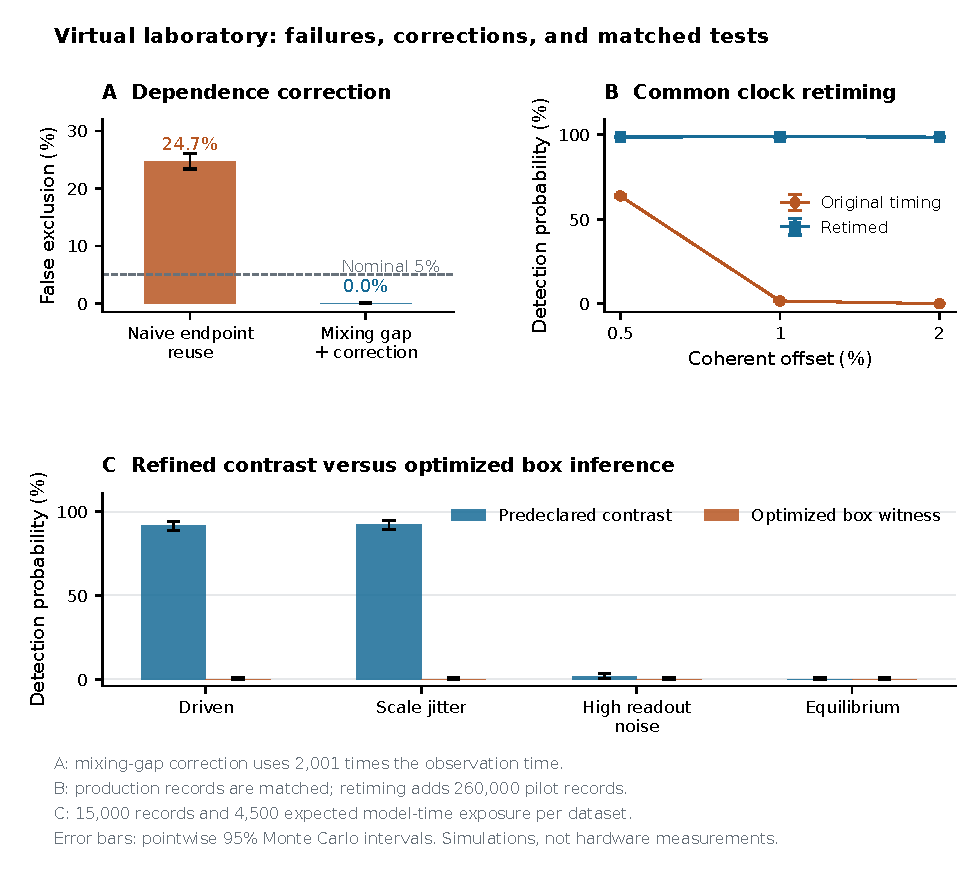
\includegraphics[width=\textwidth]{figures/virtual_laboratory.pdf}
\caption{Virtual-laboratory hardening under declared model and apparatus
contracts. Dependence corrections reduce false exclusions while increasing
sampling time. A common clock calibration repairs selected coherent-control
errors with an explicitly charged pilot. The lower panel compares the revised
fixed contrast and optimized moment-box procedure on identical 15,000-record
datasets. Error bars are pointwise Monte Carlo intervals. These are simulated
experiments; the panels have different access and cost contracts.}
\label{vl:summary-figure}
\end{figure}

\section{What is ready for physical transfer}
The transferable output is a procedure: specify the physical record, check
clock and exposure compatibility, justify conditional sampling envelopes,
freeze a targeted contrast or retain an exploratory joint region, and report
a certificate with its cost and failure controls. Exact simulator checks,
retained synthetic records and independent implementations make that procedure
inspectable by another researcher.

The next physical test should measure detector memory and exposure behavior,
validate stationarity or a preparation budget, and establish a time and energy
calibration before interpreting a positive bound. Matched comparisons should
include existing thermodynamic estimators when their required records are
actually available. The present endpoint-only experiments cannot establish
superiority over methods supplied with richer transition or waiting-time data.
Historical priority of the particular operational synthesis and physical
confirmation remain open.

\chapter{What additional calibration can buy}
\label{ci:entry}

Detecting a departure from equilibrium and measuring total dissipation are
different tasks. The previous virtual laboratories made detection more
reliable. The next question is which further observations make a physical
requirement stronger, and which missing information remains inaccessible even
after the statistics improve.

This development follows that question through a complete chain. A calibrated
detector variance shrinks the family of reversible explanations. A nonlinear
information projection measures separation from that smaller family, with
independently checked upper and lower bounds on the numerical relaxation.
A separately calibrated transition-activity cap strengthens the conversion
from record information to required entropy production. Sequential learning
and dependent-record methods address the cost of collecting the evidence.
Explicit countermodels identify the conclusions these improvements cannot buy.

The record-information argument also transfers to a stated class of stationary
overdamped diffusions. Its path-probability identity follows from established
stochastic calculus, while the reversible comparison retains the same positive
spectral structure. This extends the applicable dynamics beyond finite jump
networks. The additional finite-jump activity bound has a narrower domain and
is not transferred to a diffusion by renaming its parameters.

\section{Three boundaries that should not be conflated}
The first boundary is observational. Two physical mechanisms may produce
identical accessible records. More samples cannot distinguish those exact
alternatives. The second is statistical: different record laws may be too
close at the available precision or acquisition budget. The third is a
physical inverse problem: a sharp information certificate need not equal the
smallest entropy production compatible with every dynamical constraint.
Improving an optimization algorithm addresses none of these boundaries by
itself.

The new calibration results supply a concrete example of the first boundary.
Finite positive-lag binary pairs can agree exactly while the detector's
conditional second moment differs. Genuine additional calibration can
therefore change which explanation is admissible. A noisy analog record can
sometimes provide a useful upper variance bound without being a perfect
measurement of the hidden state.

The upper-dissipation obstruction is stronger. A connected four-state cycle
can expose every jump time while concealing the directional marks carrying
its entropy. Even complete microscopic records of bounded duration cannot
uniformly furnish finite upper entropy bounds over models with arbitrarily
rare reverse transitions. This is not a universal cap on scientific data.
It is a target-specific limitation with explicit access and calibration
repairs.

\section{From proofs to acquisition choices}
Calibrated comparison methods, longer observation windows, more readouts and
additional control information have different physical costs. The experiments
therefore report time and readout counts separately. A hypothetical conversion
between these resources is labeled as such; unmeasured hardware expenditure
is not assigned zero cost. Failed regimes and stronger comparators remain in
the evaluation.

The last step moves beyond simulated data. Publicly released optical-tweezer
trajectories are loaded with verified provenance and analyzed using the same
access questions. Their descriptive correlations and detector comparisons
are genuine reanalyses of existing measurements. The available metadata do
not establish all premises of a thermodynamic confidence certificate, so the
analysis records that limitation instead of manufacturing a dissipation claim.
The result is a precise account of what the next laboratory calibration must
supply.

The broad contribution remains operational: connect accessible evidence to
what every admissible physical explanation requires, expose the assumptions
that make the connection valid, and construct the next measurement when those
assumptions are insufficient. Established probability, spectral and
thermodynamic ingredients are credited throughout. Historical priority of the
specific synthesis and independent physical confirmation remain open.

\section{Choosing the next observation}
The most useful next step depends on the obstruction already established.
The following sequence makes that diagnosis explicit.
\begin{enumerate}
\item Specify the target. Detecting departure from detailed balance, lower
bounding entropy production, and upper bounding total entropy are distinct
inverse problems. A method adequate for the first can fail at the other two.
\item Validate the observation contract. Establish how the detector responds,
whether readings disturb the state, how time is recorded, and which source
of independence or dependence control justifies the statistical calculation.
If those conditions are missing, collect calibration evidence before
interpreting a positive contrast physically.
\item Test whether additional access removes an exact ambiguity. Same-state
twins, bounded analog values, directional transition marks and controlled
interventions reveal different information. More repetitions of an exactly
uninformative record cannot substitute for the missing observation.
\item Use all the retained evidence under a valid confidence construction.
A predeclared joint contrast can combine calibration and dynamics. A
nonlinear projection can extract a stronger bound from a covered region.
Predictable sequential tests can stop when sufficient evidence accumulates.
Their conclusions remain limited by the physical comparison theorem.
\item Compare acquisition designs using the resources the apparatus actually
consumes. Report evolution time and readout count before converting to
energy. A microscopic activity cap can sharpen a bound on dissipation; it
does not measure detector power, laser expenditure or initialization work.
\end{enumerate}

This is also a way to decide when a branch is finished. An exact compatible
countermodel settles an impossibility claim for its stated record class.
A covered positive certificate settles a conditional lower-bound claim.
Neither establishes the complete hidden dynamics. A physical application is
complete only when the apparatus supports the premises and the result answers
the stated target at the required precision.

\begin{figure}[p]
\centering
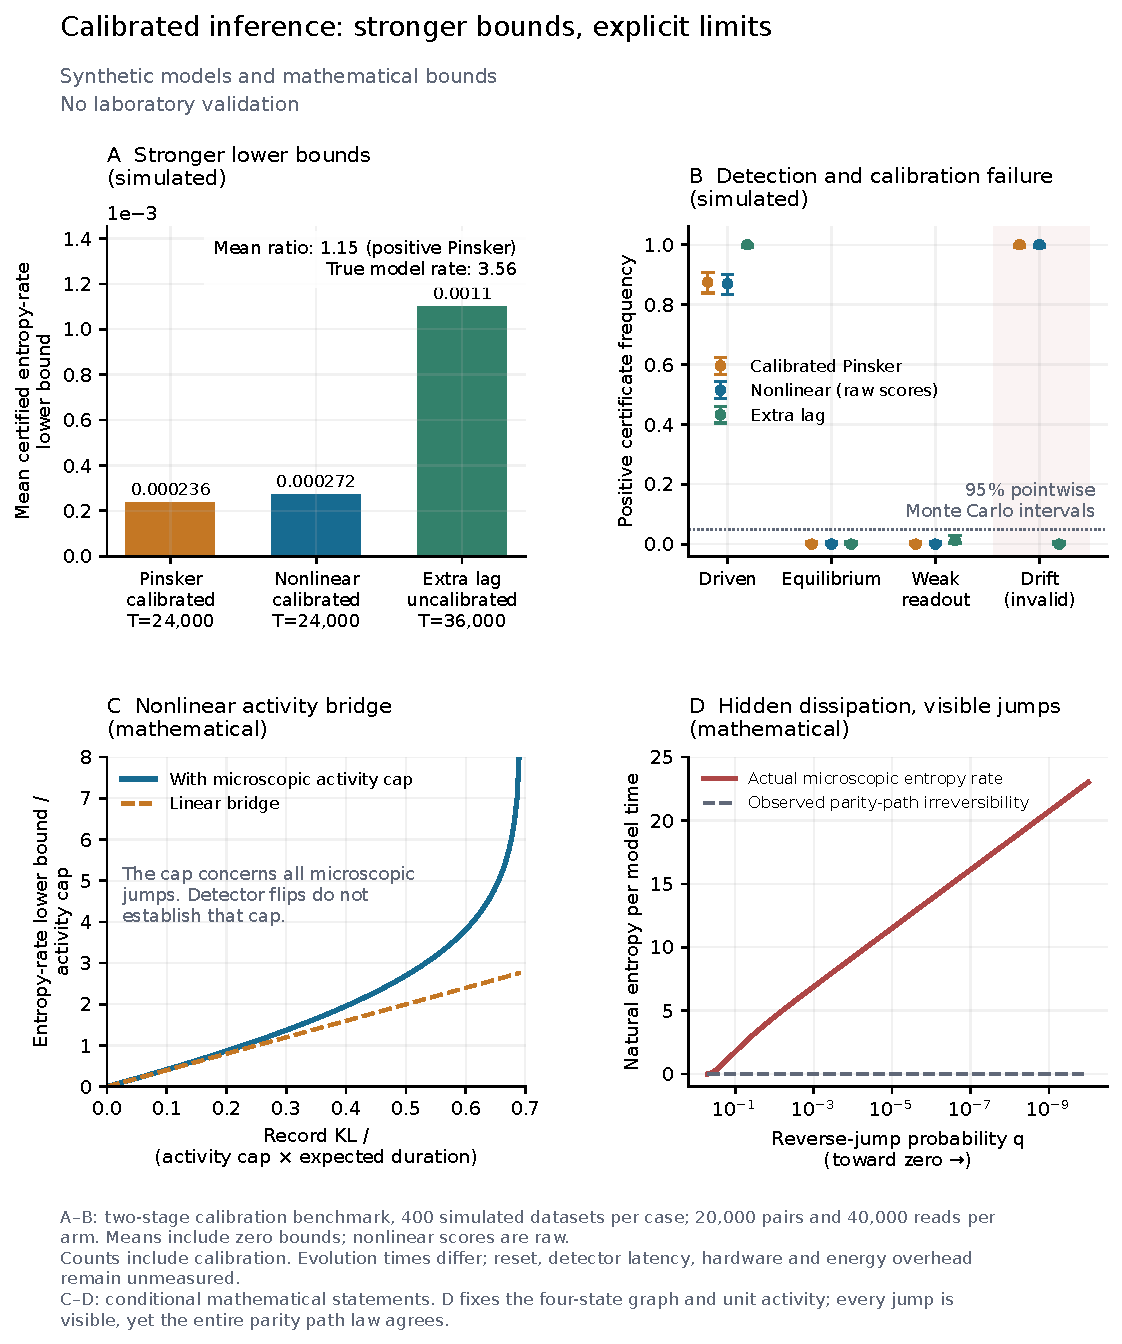
\includegraphics[width=\textwidth]{figures/calibrated_inference.pdf}
\caption{Calibrated inference and its limitations. The panels distinguish
an exact physical boundary, numerical information bounds and finite simulated
comparisons. The underlying records, equations and uncertainty calculations
are supplied in the following chapters and the release.}
\end{figure}
\begin{figure}[p]
\centering
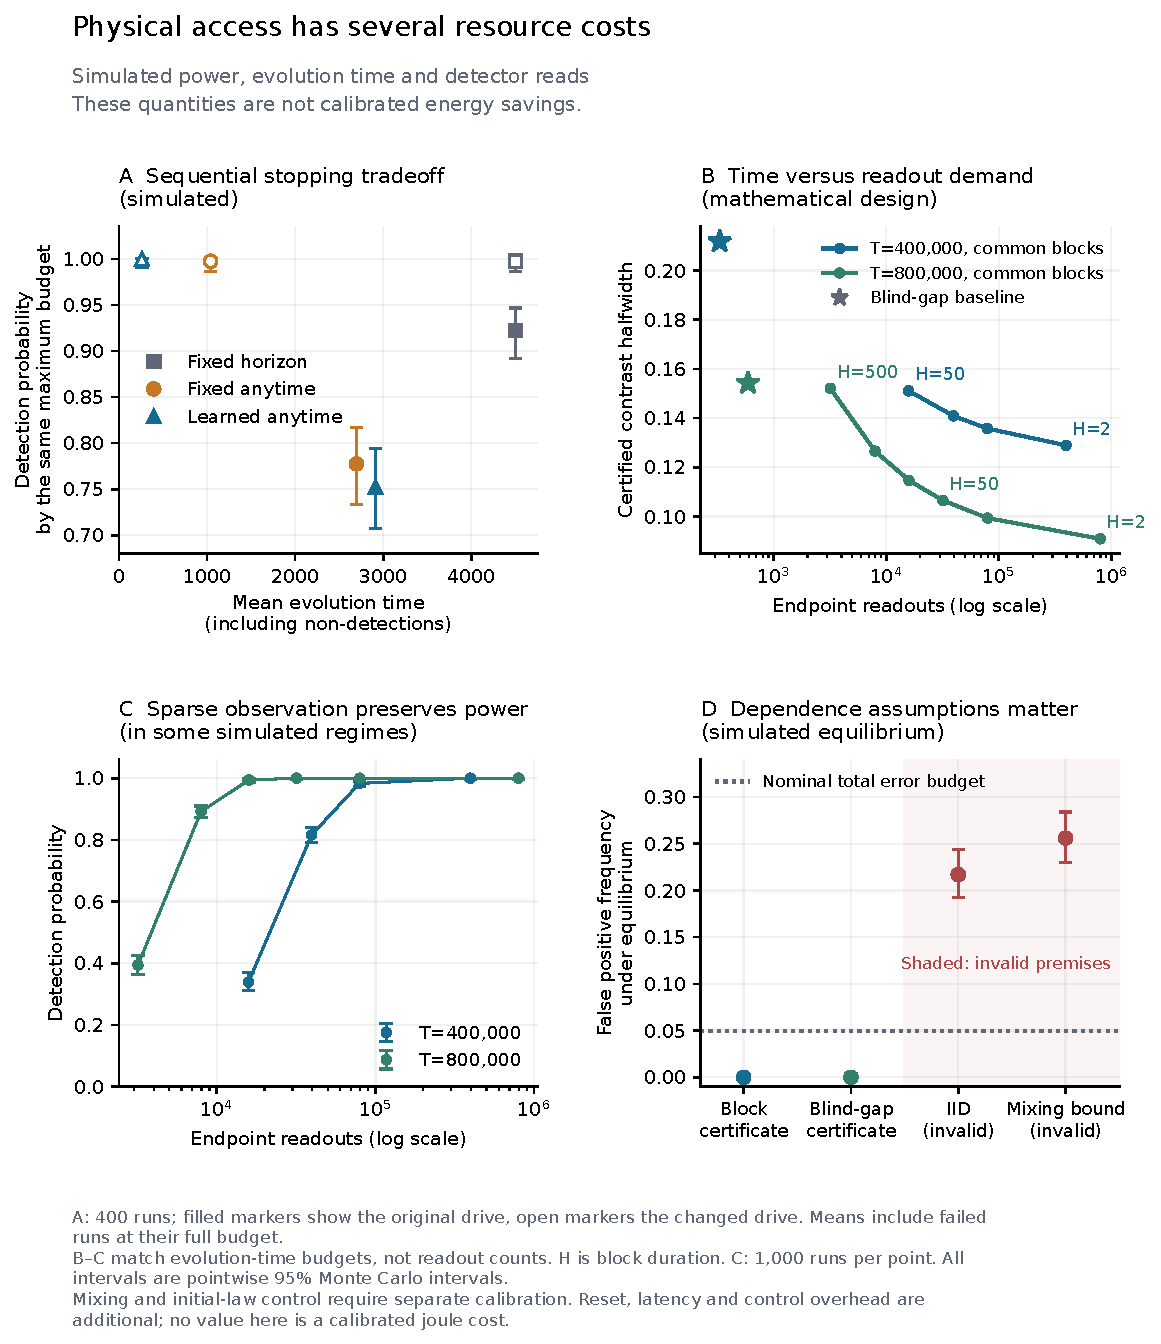
\includegraphics[width=\textwidth]{figures/calibrated_resources.pdf}
\caption{Acquisition choices at declared time and readout budgets. Each
simulated comparison is restricted to its frozen design. Faster stopping or
fewer readings does not imply a measured energy saving, and deliberately
invalid calibration controls remain part of the evaluation.}
\end{figure}

\chapter{Detector calibration and the zero-lag access boundary}
\label{ch:ci-calibration}

The size of an observed fluctuation depends on the detector as well as on the
physical process. Calibrating that dependence can reveal irreversibility in a
positive, monotonically decreasing correlation, before a negative correlation
or revival appears. The same analysis also identifies a limit: arbitrarily
precise measurements at a fixed positive-lag pair menu need not determine the
calibration quantity itself.

\section{The conditional second moment}
Let a fixed, noninvasive binary detector have conditional mean
$f_i=\mathbb E[Y\mid X=i]\in[-1,1]$. Under the stationary law $\pi$, define
\begin{equation}
 m=\sum_i\pi_i f_i,\qquad A=\sum_i\pi_i f_i^2,
 \qquad u=m^2,\qquad0\leq u\leq A\leq1.
 \label{eq:ci-mA}
\end{equation}
Two readings with conditionally independent noise at the same unchanged hidden
state obey
\begin{equation}
 \mathbb E[Y^{(1)}Y^{(2)}]=A,
 \qquad\Pr(Y^{(1)}=Y^{(2)})=\frac{1+A}{2}.
 \label{eq:ci-zero-lag}
\end{equation}
Squaring one binary reading instead gives $Y^2=1$ and does not measure $A$.
The two readings are generally dependent through their common hidden state.

For an instantaneous detector, $m$ and $A$ agree under $Q$ and its additive
reversibilization because $\pi$ and $f$ are unchanged. This transfer need not
hold for nonlinear finite-exposure path functionals. A deterministic binary
state detector already has $A=1$. If $f(X)$ itself is reliably observed, its
square directly measures $A$; this is additional access, outside the binary-only
obstruction proved below.

\section{Bounded analog observations supply an upper calibration}
A trusted instantaneous analog record can improve the comparison class even
without a same-state replicate. Let $Z\in[-1,1]$ be the output of a fixed,
noninvasive memoryless channel, and write $f_i=\mathbb E[Z\mid X=i]$. Then
\begin{equation}
 m=\mathbb E Z,\qquad
 A=\mathbb E f(X)^2\leq B:=\mathbb E Z^2,
 \qquad B-A=\mathbb E\operatorname{Var}(Z\mid X).
 \label{eq:ci-analog-upper}
\end{equation}
At distinct times, conditionally independent readout noise gives
$\mathbb E[Z_0Z_t]=\langle f,e^{Qt}f\rangle_\pi$. Thus a valid upper confidence
bound on $B$ is also an upper bound on $A$. A lower bound on $B$ does not transfer.
Both $m$ and $B$ are unchanged under the additive reversible reference because
its stationary law and instantaneous detector channel are the same.

For example, let $Z=X/4+\epsilon/2$, with independent fair signs $X,\epsilon$.
Then $A=1/16$ while $B=5/16$. The observable second moment gives a useful upper
bound, but it is not the latent conditional second moment. Randomizing two
binary encodings from the same noisy $Z$ gives product mean $B$, not $A$, because
they share the analog measurement noise. Independently encoding readings at
distinct times is compatible with the correlation model.

The API accepts any valid simultaneous bounds on $m$ and $B$ and sets
$A\in[0,B_U]$. Its optional iid summary helper uses a two-sided Hoeffding bound
for the mean and a one-sided bound for the squared observation. A dependent
trajectory requires a separate valid calibration procedure; the iid helper
cannot be applied to every raw sample merely because the detector noise is
memoryless. Neither this upper-bound transfer nor the earlier exact transfer
is automatic for nonlinear finite-exposure functionals.

\section{A sharp calibrated reversible class}
For commensurate positive lags $k\Delta$, define
\begin{equation}
 \mathcal M_{m,A}=\left\{
 q_k=\frac{1+u+(A-u)\int_0^1x^k\,\mu(dx)}2:
 \mu\text{ a probability measure}\right\}.
 \label{eq:ci-calibrated-cone}
\end{equation}

\begin{theorem}[Sharp calibrated comparison class]
For a finite menu of positive integer lag indices, the closure of the agreement
vectors of finite stationary reversible chains with detector mean $m$ and
conditional second moment $A$ is exactly $\mathcal M_{m,A}$. The closure is
unchanged if the approximating chains must be irreducible.
\end{theorem}
\begin{proof}
Necessity follows from the established reversible spectral representation:
$C(t)=m^2+\sum_\ell b_\ell e^{-\lambda_\ell t}$, with
$b_\ell\geq0$ and $\sum_\ell b_\ell=A-m^2$~\cite{vlAldousFill2002}.
Additional conserved modes can be included at $\lambda=0$.

For sufficiency, a finite moment vector has an atomic representing measure
with at most $K+1$ atoms, where $K$ is the number of measured coordinates. If
$A=m^2$, use a constant detector. Otherwise put
\[
 a=\frac{m-A}{1-m},\qquad r=\frac{m-a}{1-a}.
\]
Then $-1\leq a<m<1$ and $0<r<1$. A two-state block with stationary law
$(r,1-r)$, detector values $(1,a)$, and generator
\[
 Q_x=\frac{-\log x}{\Delta}(\boldsymbol1\pi-I)
\]
has mean $m$, second moment $A$, and correlation
$m^2+(A-m^2)x^k$. Mix such blocks with the desired atomic weights. Replace any
atom $x=0$ by positive atoms approaching zero. Finally add
$\varepsilon(\boldsymbol1\pi-I)$ to the full generator. This preserves
$\pi,m,A$, makes the model irreducible and converges to the required moments as
$\varepsilon\downarrow0$.
\end{proof}

The sharpness statement concerns deterministic commensurate lags. A compatible
random-clock family preserves this calibrated set as an outer comparison class,
but its particular clock law can impose further restrictions.

\section{Calibration uncertainty and exact support}
A simultaneous interval for $m$ maps to an interval $[u_L,u_U]$ for $m^2$.
Its lower endpoint is zero if the mean interval crosses zero; otherwise use the
smaller squared endpoint. Together with $A\in[A_L,A_U]$, this produces the
exact polygon
\[
 \mathcal P=([u_L,u_U]\times[A_L,A_U])\cap\{0\leq u\leq A\leq1\}.
\]
For a contrast $c=(c_k)$, write $S_c=\sum_kc_k$ and
$p_c(x)=\sum_kc_kx^k$. Its reversible support is
\begin{equation}
 \sup_{q\in\mathcal M_{\mathcal P}}\sum_kc_kq_k
 =\frac12\max_{(u,A)\in\operatorname{vert}\mathcal P}
 \left[(1+u)S_c+(A-u)\max_{0\leq x\leq1}p_c(x)\right].
 \label{eq:ci-support}
\end{equation}
The full class is the convex hull of the vertex curves. A mixture has effective
parameters in $\mathcal P$, and reweighting its atomic measures by $A-u$ gives
another admissible measure. The implementation uses exact rational Bernstein
bounds for the continuous polynomial maximum; a numerical grid is only a lower
comparison.

For fixed $m$, these closed positive-lag classes are nested in $A$: extra
variance can be placed at $x=0$. Thus an upper calibration of $A$ sharpens the
comparison set. A lower calibration alone does not force visible variance when
arbitrarily fast hidden modes are allowed.

For $N$ independent same-state pair records, the count table gives
\[
 \widehat m=\frac{n_{++}-n_{--}}N,\qquad
 \widehat A=\frac{n_{++}+n_{--}-n_{+-}-n_{-+}}N.
\]
Both are averages of $N$ variables in $[-1,1]$. Hoeffding and a union bound give
a simultaneous radius
$\sqrt{2\log(4/\alpha)/N}$~\cite{caHoeffding1963}. This does not treat the
$2N$ readings as independent. Calibration error probability must be combined
with the subsequent inference guarantee. An empty physical calibration region
is reported explicitly rather than converted into an entropy estimate.

\section{Detecting excessively steep positive decay}
Since $x-x^2\leq1/4$, every calibrated reversible model satisfies the sharp bound
\begin{equation}
 q(t)-q(2t)\leq\frac{A-m^2}{8}.
 \label{eq:ci-steep-decay}
\end{equation}
A two-state block with $x=1/2$ attains it. This is a restriction on the rate of
change relative to the calibrated fluctuation amplitude, not merely on whether
the correlation is positive or decreasing.

Consider a synthetic four-state cycle with clockwise rate three, reverse rate
one and conditional detector means $(1/2,1/2,-1/2,-1/2)$. Its stationary law is
uniform, $m=0$, $A=1/4$, and
\[
 C(t)=\frac14 e^{-4t}\cos(2t).
\]
At $t=7/40$, exact series enclosures certify
\[
 q(t)-q(2t)>0.03473386533798
 >\frac1{32}=0.03125.
\]
Both correlations are positive and decrease. The uncalibrated support ceiling
$1/8$ does not detect this example. Its true generator entropy rate is
$2\log3$; that known model value is distinct from any lower bound inferred from
its restricted records. This is a population certificate, not sampled
experimental evidence.

\section{Exact positive-lag ambiguity}
\begin{theorem}[Finite pair menus do not identify the missing spectral mass]
For every integer $K\geq1$, there are finite irreducible reversible models with
zero detector mean, identical stationary binary-pair laws at each lag
$1,\ldots,K$, and different values of $A$.
\end{theorem}
\begin{proof}
Choose $x_j=j/(K+2)$ and $v_j=(-1)^j{K+1\choose j}$ for
$j=1,\ldots,K+1$. Finite differences give
\[
 \sum_{j=1}^{K+1}v_jx_j^k=0\quad(1\leq k\leq K),
 \qquad \sum_{j=1}^{K+1}v_j=-1.
\]
Split positive and negative coefficients and scale their magnitudes by
$s=(2^{K+1}-1)^{-2}$. The two positive spectral measures have equal measured
moments and unequal total mass.

For either measure, use independent symmetric telegraph coordinates $Z_j$ with
correlation $x_j^t$, and detector mean
$f(Z)=\sum_j\sqrt{s|v_j|}\,Z_j$. Its absolute value is at most one because the nonzero $|v_j|$ are integers,
so $\sqrt{s}\sum_j\sqrt{|v_j|}\leq\sqrt{s}\sum_j|v_j|\leq1$. The product chain is finite and irreducible, and its
correlation is exactly the desired spectral sum. Its mean is zero. The binary
pair law is $(1+abC(t))/4$ for outputs $a,b\in\{-1,1\}$, so the measured laws
agree exactly while $A=C(0)$ differs.
\end{proof}

For a small explicit example, compare spectral weights $3/16$ at $x=1/4$ and
$1/16$ at $x=3/4$ with weight $3/16$ at $x=1/2$. Their second moments are
$1/4$ and $3/16$, but both give $C(1)=3/32$ and $C(2)=3/64$. They have
irreducible four-state and two-state realizations, respectively, with exit rates
below one. Even a finite rate cap therefore does not imply exact identification
from an unchanged finite pair menu.

The result does not equate their full time-resolved trajectories or all
higher-order temporal records. Those observations, a known detector law or
true same-state calibration supply additional access. Repeating the unchanged
pair measurements cannot remove their exact ambiguity.

\section{Fast modes and the quantitative kinetic repair}
A second obstruction concerns uniform precision over unknown rates. Compare
independent fair binary outputs with a reversible two-state model having
correlation $Ae^{-\lambda t}$. Their pair total variation distance is
$Ae^{-\lambda t}/2$. For $N$ independent records at lags at least $t_{\min}>0$,
\begin{equation}
 \operatorname{TV}(P_0^{(N)},P_\lambda^{(N)})
 \leq\frac{NA}{2}e^{-\lambda t_{\min}}.
 \label{eq:ci-fast-mode}
\end{equation}
An order-one difference in $A$ can therefore be hidden at any finite precision
by a sufficiently fast reversible mode. Every model in this comparison has
zero stationary entropy production. For any finite independent clock menu with
no atom at zero, dominated convergence gives the same conclusion using
$\mathbb E e^{-\lambda T}$. Exact continuum data with unlimited precision are
a different observation contract.

A calibrated kinetic bound permits a controlled approximation. For any stationary
finite Markov chain, including a nonreversible one,
\begin{equation}
 A-C(t)=\frac12\mathbb E[(f(X_t)-f(X_0))^2].
\end{equation}
If every exit rate is at most $\Lambda$, then
\begin{equation}
 0\leq A-C(t)\leq2(1-e^{-\Lambda t}).
 \label{eq:ci-rate-repair}
\end{equation}
Indeed the integrand is at most four and vanishes when no jump occurs.
A bound $J$ on stationary jump activity similarly gives $A-C(t)\leq2Jt$.
These bounds make delayed calibration uniformly accurate as the accessible
delay approaches zero. They do not promise exact identification at fixed
positive lags. An energy-dissipation bound alone cannot supply either kinetic
bound: arbitrarily fast reversible chains dissipate no stationary heat.

Finally, the same-state noise premise is testable only with additional apparatus
knowledge. Conditionally anti-correlated readouts can each have means
$\pm1/2$ while their product has mean zero, although $A=1/4$. For example use
conditional count proportions $(1/2,1/4,1/4,0)$ and
$(0,1/4,1/4,1/2)$. An apparently feasible calibration can then be too small and
falsely reject an equilibrium record. Marginal counts alone do not establish
conditional independence or absence of measurement backaction.

The ingredients of this chapter---reversible spectral mixtures, truncated
moments, replicate covariance and concentration---are established. The scoped
advance is their integration into a sharp calibrated comparison class, an
executable confidence contract and explicit physical countermodels marking the
remaining access boundary. Historical originality and empirical validation
remain separate questions.

\chapter{Quantitative inference with certified nonlinear bounds}
\label{chap:ci-nonlinear}

A positive contrast answers whether the specified equilibrium comparison class
can explain the observations. Its quadratic entropy bound can discard much of
the available probability information. This chapter gives a nonlinear replacement
and an independently checkable bracket on the resulting optimization problem.
It also identifies a second source of looseness: even an exact observational
KL projection need not determine physical dissipation. An additional calibration
of microscopic jump activity can sharpen that separate physical step.

The variational representation of relative entropy, convex information
projection and likelihood-score testing are established ingredients. The
modern composite-null testing literature gives closely related log-optimal
score constructions\cite{ciLarsson2025,ciGrunwald2024,ciLarsson2026}. The
contribution here is their explicitly certified use with a calibrated continuous
moment class, a nonrectangular finite-data confidence region, and a separate
physical-resource calculation. Simulations and numerical optimization do not
establish the physical premises.

\section{The comparison problem and its scope}
Let $k_1,\ldots,k_m$ be positive integer lag indices, $w_i>0$ sum to one, and
$t_i>0$ bound the full expected path duration associated with each target
record. Write $p_i$ for the probability that the two binary readings agree.
Suppose a valid joint confidence event places the target vector in
\[
 {\cal P}=\{p\in\textstyle\prod_i[\ell_i,h_i]:a\cdot p\ge b\}.
\]
The contrast $a$ must have been declared before its test records, or selected
using independent pilot data. The halfspace can use the one-sided conditional
Hoeffding bound proved in the preceding work; the default box is $[0,1]^m$.
An empty region is rejected as an inconsistent input, not interpreted as a
scientific certificate.

Let $V$ be rational vertices of a calibrated polygon in
$\{(u,A):0\le u\le A\le1\}$. Here $u$ bounds the square of the stationary
detector mean and $A$ bounds the stationary second moment of its conditional
mean. Define the closed reversible comparison class
\[
 {\cal K}_V=\operatorname{conv}\left\{
  q_i={1+u+(A-u)x^{k_i}\over2}:(u,A)\in V,\ 0\le x\le1\right\}.
\]
The preceding calibration chapter explains the access needed to measure $A$.
The convex-hull representation allows distinct spectral atoms and arbitrary
calibration points inside the polygon. Indeed, a convex combination has
effective $u=\sum_j\theta_j u_j$, $A=\sum_j\theta_j A_j$, and spectral weights
proportional to $\theta_j(A_j-u_j)$. Conversely, decomposing $(u,A)$ into
vertices gives such a convex mixture. The atom $x=0$ is part of the closed
comparison class and may represent an infinite-rate limit; it need not be
an exact finite-rate physical realization.

The quantity to bracket is
\begin{equation}
 B({\cal P},{\cal K}_V;w)=
 \inf_{p\in{\cal P},q\in{\cal K}_V}
       \sum_i w_i\,\operatorname{kl}(p_i\Vert q_i),
 \label{eq:ci-nonlinear-projection}
\end{equation}
where $\operatorname{kl}$ is Bernoulli relative entropy in nats. For a
stationary ordinary-reversal CTMC, the earlier additive-reversibilization
bridge gives
\[
 \sigma\ge {4B\over\sum_iw_it_i}.
\]
This comparison class generally contains reference models that cannot be the
additive reversibilization of the same hidden generator producing $p$.
Consequently, $B$ is an observational relaxation. A feasible upper bound on
$B$ is not an upper bound on physical entropy production, or proof that its
lower bound is physically attainable. Odd-variable physical reversal,
measurement disturbance and an uncalibrated initial transient remain outside
this stationary interpretation.

\section{An exact dual certificate and a primal bracket}
Choose arbitrary positive rational scores $h_{i0},h_{i1}$. Let
\begin{align*}
 L(h)&=\inf_{p\in{\cal P}}\sum_iw_i
       [(1-p_i)\log h_{i0}+p_i\log h_{i1}],\\
 U(h)&=\sup_{q\in{\cal K}_V}\sum_iw_i
       [(1-q_i)h_{i0}+q_i h_{i1}].
\end{align*}
Then
\begin{equation}
 B\ge\max\{0,L(h)-\log U(h)\}.
 \label{eq:ci-nonlinear-dual}
\end{equation}
For each fixed pair $(p,q)$, regard $(i,y)$ as a joint record with probabilities
$w_i\operatorname{Ber}(p_i)_y$ and $w_i\operatorname{Ber}(q_i)_y$.
The relative-entropy variational inequality gives
$D(P\Vert Q)\ge E_P\log h-\log E_Qh$.
Taking the worst cases over the two convex sets proves
\eqref{eq:ci-nonlinear-dual}.

Both optimization steps in a supplied certificate are checked on their whole
domains. For a calibration vertex $(u,A)$, the normalization is the maximum on
$[0,1]$ of the rational polynomial
\[
 \sum_iw_i\left[h_{i0}+(h_{i1}-h_{i0})
       {1+u+(A-u)x^{k_i}\over2}\right].
\]
Rational Bernstein coefficients after interval subdivision give a rigorous
upper bound. No sampling grid is used as a proof of this maximum.
The logarithms are enclosed by the inherited rational atanh-series routine.
Substituting their lower endpoints gives a linear lower objective on
${\cal P}$. Its minimum is an exact fractional-knapsack calculation: begin
at a box minimizer, and if the contrast constraint fails, move coordinates in
the direction increasing $a\cdot p$, ordered by objective cost per unit
increase. These rational moves attain the minimum of the enclosed linear
objective. The continuous normalization and outward logarithm enclosures then
give a rational lower bound on $B$.

Conversely, supply rational $p\in{\cal P}$ and finitely many rational atoms
$(v_j,x_j,\theta_j)$ with $v_j\in V$, $x_j\in[0,1]$, $\theta_j\ge0$ and
$\sum_j\theta_j=1$. They produce an exactly feasible $q\in{\cal K}_V$.
Upper logarithm enclosures give
\[
 B\le\sum_iw_i\operatorname{kl}(p_i\Vert q_i)\le B_{\rm upper}.
\]
Thus the reported gap $B_{\rm upper}-B_{\rm lower}$ measures the remaining
uncertainty of the relaxation calculation. The numerical optimizer proposes
scores and mixtures; the rational checks retain their validity even when it
fails to converge or uses a coarse proposal grid.

For an interior minimizing pair $(p^*,q^*)$, the dual has no gap. Set
$h_{i1}=p_i^*/q_i^*$ and
$h_{i0}=(1-p_i^*)/(1-q_i^*)$. First-order optimality in $q$ implies
$E_Qh\le1$ for all comparison vectors, with equality at $q^*$.
First-order optimality in $p$ implies
$E_P\log h\ge E_{P^*}\log h$ throughout ${\cal P}$. Substitution gives
equality in \eqref{eq:ci-nonlinear-dual}. Boundary minimizers can require
limiting scores; the implementation claims only the brackets it actually
checks, not attainment at finite scores in every case.

For a fixed alternative, normalizing $h$ by $U(h)$ gives a nonnegative score
with expectation at most one throughout the composite equilibrium null.
Its expected logarithm is the familiar information-projection testing
objective. This connection does not make a score fitted to its own data an
automatically valid significance test. Here data-dependent scores are safe
because they are minimized over a previously valid confidence region that
contains the entire true probability vector on the same event. Calibration
failure probabilities must be included in that event separately.

\section{A realizable calibration example}
Consider a stationary twenty-state ring with conditional detector mean
$f_j=\cos(2\pi j/20)$. Its uniform stationary law gives $m=0$, $A=1/2$.
Put $r=\sqrt{497}/25$, $\omega=\arccos(19/\sqrt{497})$,
$\gamma=-\log r$, and $\phi=2\pi/20$. Choose clockwise and anticlockwise
rates
\[
 a={1\over2}\left({\gamma\over1-\cos\phi}
                   +{\omega\over\sin\phi}\right),\qquad
 b={1\over2}\left({\gamma\over1-\cos\phi}
                   -{\omega\over\sin\phi}\right).
\]
Both are positive: numerically $a\simeq2.06125923$ and $b\simeq0.27982488$.
Independent binary readings with means $f_j$ have agreement probability
$p(t)=1/2+e^{-\gamma t}\cos(\omega t)/4$. The specified constants give
$p(1)=0.69$, $p(2)=0.59$ exactly. The predeclared contrast
$(38/25,-1)$ therefore takes the value $1147/2500=0.4588$.
Its calibrated reversible support is
$19/25-1/2+(19/25)^2/4=0.4044$; allowing $A$ to rise to one raises
that support to $0.5488$. Positive and decreasing correlations alone do not
expose the discrepancy; their scale relative to calibrated detector variance
does.

Using the idealized confidence halfspace with threshold $0.4588$, equal
mixture weights and durations $(1,2)$, the saved deterministic calculation
brackets the calibrated record-KL relaxation between
$0.0010251000031$ and $0.0010265638733$. The uncalibrated bracket is
$[0,6.43\times10^{-14}]$. These are model calculations, not finite-record
experimental confidence statements. The true model entropy rate is about
$3.55736$, whereas the certified lower rate is about $0.002734$.
The narrow optimization bracket therefore reveals a substantial evidential
and physical-bridge limitation, not an unresolved numerical calculation.

\section{The physical bridge has its own limit}
For an unordered edge, put
$a=\pi_iq_{ij}$, $b=\pi_jq_{ji}$, $c=a+b$, and
$x=|a-b|/(a+b)$. Edges with zero traffic contribute zero. For finite entropy
assume positive reverse flux whenever forward flux is positive. Define
\[
 j(x)={ (1+x)\log(1+x)+(1-x)\log(1-x)\over2},
 \qquad e(x)=x\log{1+x\over1-x}.
\]
The path-KL rate from $Q$ to $S=(Q+Q^*)/2$ and the entropy-production rate are
exactly
\[
 d=\sum_{\{i,j\}}c_{ij}j(x_{ij}),\qquad
 \sigma=\sum_{\{i,j\}}c_{ij}e(x_{ij}).
\]
The escape rates of $Q$ and $S$ agree pointwise, so there is no omitted
waiting-time term in $d$. Total stationary microscopic jump activity is
$K_0=\sum c_{ij}$.

As $x\to1$, $j(x)\to\log2$ while $e(x)\to\infty$. A fixed-activity driven
ring therefore has bounded path-KL rate but unbounded entropy production.
An arbitrarily accurate endpoint projection cannot eliminate this physical
loss of information. The data do not determine a finite upper bound on total
dissipation without further assumptions.

There is, however, a sharper lower bridge if a separate physical calibration
gives $K_0\le K$. Write $G=e\circ j^{-1}$ on $[0,\log2)$. Then
\begin{equation}
 \sigma\ge K\,G\left({B\over K\bar t}\right),
 \qquad \bar t=\sum_iw_it_i,
 \quad 0\le {B\over K\bar t}<\log2.
 \label{eq:ci-activity-bridge}
\end{equation}
To prove it, $j'(x)=\operatorname{atanh}x$ and
\[
 {e'(x)\over j'(x)}
 =2+{2x\over(1-x^2)\operatorname{atanh}x}
\]
increase strictly for $0<x<1$. The derivative of the second term has the
sign of $(1+x^2)\operatorname{atanh}x-x$, which is positive because its
value at zero is zero and its derivative is
$2x\operatorname{atanh}x+2x^2/(1-x^2)>0$.
Thus $G$ is increasing and convex, with $G(0)=0$ and $G'(0)=4$.
Jensen's inequality gives $\sigma\ge K_0G(d/K_0)$.
The perspective $K\mapsto KG(d/K)$ is nonincreasing: convexity gives
$G(z)-zG'(z)\le0$. Finally data processing gives $d\ge B/\bar t$.
These three inequalities prove \eqref{eq:ci-activity-bridge}.
It improves $\sigma\ge4B/\bar t$, with strict improvement for nonzero
evidence and finite activity cap except for numerical rounding.

The activity-calibrated envelope is sharp for full-path observations of a
uniform ring with clockwise and anticlockwise rates
$K(1+x)/2$ and $K(1-x)/2$: every edge has the same bias, the stationary law is
uniform, total activity equals $K$, and Jensen is an equality. This is a
sharpness statement about the full-path physical bridge. Restricted endpoint
observations usually lose information, and the moment relaxation can lose
more; no endpoint sharpness follows from the ring example.

After normalization by activity, $d/K_0$ is the Jensen--Shannon divergence
between the stationary directed-flux distribution and its transpose, while
$\sigma/K_0$ is half their Jeffreys divergence when Jeffreys is defined as
the sum of the two directed KL divergences. Bounds between these divergences
and general finite-support optimization methods are established
\cite{ciCrooks2008,ciFalasco2022,ciGuntuboyina2014}. The explicit envelope
above is proved here for this inference contract; historical priority of the
scalar divergence inequality is not claimed.

The implementation inverts $j$ by rational bisection. If an upper logarithm
enclosure proves $j(x_-)\le B/(K\bar t)$, then
$Ke(x_-)$ with a lower logarithm enclosure is a certified lower entropy
bound. The previous linear bound is retained if it is numerically larger.
If the supplied evidence exceeds $K\bar t\log2$, the routine reports an
incompatible joint contract rather than an entropy estimate. The microscopic
activity cap cannot be inferred from a count of coarse detector changes:
unobserved jumps still contribute activity. Its measurement cost, preparation
cost and timing calibration belong in the experimental resource account.

\section{A scoped transfer to overdamped diffusions}
The observational certificate is not restricted to a finite state space.
Consider the stationary diffusion
\[
 dX_t=b(X_t)\,dt+\sqrt{2D}\,dW_t
\]
on a connected compact periodic domain, with smooth drift, constant symmetric
positive-definite $D$, and smooth strictly positive stationary density $\pi$.
All state coordinates have even physical time-reversal parity. Define
\[
 b_s=D\nabla\log\pi,\qquad v=b-b_s,\qquad
 \sigma=\int v^TD^{-1}v\,\pi\,dx.
\]
This is the standard steady current expression for overdamped entropy
production under the stated physical convention\cite{ciSeifert2012}.
The reversible comparison diffusion has drift $b_s$ and the same diffusion
matrix and initial law $\pi$.

The drift likelihood formula\cite{ciGirsanov1960} gives
\begin{equation}
 D(\mathbb P_b^{[0,t]}\Vert\mathbb P_{b_s}^{[0,t]})
   ={1\over4}E_b\int_0^t v(X_s)^TD^{-1}v(X_s)\,ds
   ={t\sigma\over4}.
 \label{eq:ci-diffusion-bridge}
\end{equation}
The factor follows from the noise covariance $2D$: the control in the
Brownian likelihood is $(\sqrt{2D})^{-1}v$, and relative entropy is one half
its expected squared norm. On the compact periodic domain the drift
difference is bounded, so Novikov's condition and finite energy hold.
On a noncompact domain the conclusion instead requires nonexplosion,
the appropriate boundary or decay conditions, a valid true likelihood
martingale and finite expected energy. Novikov is a sufficient condition,
not a claim automatically valid for every linear example and every horizon.

The reference generator is
$L_s=\pi^{-1}\nabla\!\cdot(\pi D\nabla)$.
Periodic integration by parts makes it self-adjoint and nonpositive in
$L^2(\pi)$. For a fixed bounded detector conditional mean $f$, the spectral
theorem therefore gives
\[
 E_s[f(X_0)f(X_t)]
   =m^2+\int_{[0,\infty)} e^{-\lambda t}\,d\nu(\lambda),
 \quad \nu\ge0,\quad\nu([0,\infty))=A-m^2,
\]
where $m=E_\pi f$ and $A=E_\pi f^2$.
Independent noninvasive binary readout noise at the two endpoints has the
same correlation. At times $k\Delta$, putting $x=e^{-\lambda\Delta}$ yields
the calibrated moment comparison class already used above. Data processing
of \eqref{eq:ci-diffusion-bridge} proves the same record-KL lower certificate
$\sigma\ge4B/\bar t$.

This corollary composes established likelihood and spectral theory. It is not
a new physical law. It supplies a legitimate mathematical route to suitable
overdamped position measurements, including model classes used for optical
traps; it does not certify that any particular experimental dataset satisfies
the assumptions. Sharpness or finite realization within the CTMC comparison
class does not establish sharpness in a diffusion-only class. The optional
finite-jump activity envelope does not transfer to continuous diffusions.

For an independently computable check, take a two-dimensional rotational
Ornstein--Uhlenbeck process
\[
 dX_t=(-I+\omega J)X_t\,dt+\sqrt2\,dW_t,
 \qquad J=\begin{pmatrix}0&-1\\1&0\end{pmatrix}.
\]
Its stationary covariance is $I$, the reversible drift is $-x$, and
$v=\omega Jx$. Hence $\sigma=2\omega^2$ and the full-path relative entropy
to the reversible reference is $t\omega^2/2$. This unbounded linear drift
does not need a global Novikov assertion: smooth radial cutoffs of the
rotational drift have bounded likelihood controls and preserve the Gaussian
stationary density, since the rotation is orthogonal to radial gradients.
Their expected control energies are uniformly bounded by the Gaussian second
moment. The resulting likelihoods have uniformly bounded relative entropy
and are uniformly integrable. Localization, nonexplosion and uniqueness of
the linear diffusion identify the limiting true likelihood; its finite-energy
Girsanov expression gives the identity above.

Choose the bounded detector mean $f(x)=\sin(x_1)$ and independent binary
readout noise. The stationary mean is zero and
$A=(1-e^{-2})/2$. Since the two scalar Gaussian coordinates at times zero and
$t$ have correlation $\rho=e^{-t}\cos(\omega t)$,
\[
 C(t)=E[f(X_0)f(X_t)]
 =\tfrac12\{e^{-(1-\rho)}-e^{-(1+\rho)}\}
 =e^{-1}\sinh\rho.
\]
The first equality follows directly from the Gaussian characteristic function
and $2\sin x\sin y=\cos(x-y)-\cos(x+y)$.
For $\omega=2$, $t=1$, existing rational exponential and cosine enclosures
certify $C(t)<0$, hence a positive entropy lower certificate, while the same
detector and score yield zero in the $\omega=0$ equilibrium control.
The model entropy rate is exactly eight and the full-path KL is exactly two.
This is an exact Gaussian-model calculation with certified transcendental
enclosures, not a new trajectory experiment or an empirical measurement.

\section{Implementation and checks}
The API \path{constructive_access.calibrated.nonlinear.design} returns the
exact dual lower certificate, a feasible primal upper bracket, and their gap.
The faster \path{certify} accepts supplied rational scores and may reuse them
across independently constructed confidence regions.
\path{confidence_region} constructs the fixed-contrast halfspace and
\path{activity_bridge} supplies the optional activity-calibrated physical step.
All four routines distinguish an assumed observation contract from evidence
that a physical apparatus satisfies it.

The tests compare the rational linear-program solver with an independent
linear optimizer, recover an analytic Bernoulli KL projection, exercise an
equilibrium control, check off-grid normalization and reject malformed primal
points. A positive, decreasing two-lag signal is accepted by the uncalibrated
class but separated after second-moment calibration. Independent scalar root
finding checks the activity inversion, including the equal-bias ring equality
case. Deterministic example outputs are mathematical checks, not measured
laboratory data. Matched held-out performance comparisons are reported in the
integrated benchmark chapter.

\chapter{What restricted access cannot upper-bound}
\label{ch:dissipation-limits}

Sharper lower certificates do not automatically make total dissipation
identifiable. This chapter separates three obstructions: an exactly hidden
current, an identifiable parameter with a singular thermodynamic dependence,
and incomplete physical channel resolution. Its main construction uses one
connected four-state cycle. Every microscopic jump changes the detector output.
There is no independent hidden subsystem, no parallel microscopic edge, and no
unobserved transition time.

Strong lumpability and loss of entropy production under coarse-graining are
established results~\cite{ac_buchholz,ciBusiello2019}. Optimizing over compatible
hidden mechanisms is also an established approach to sharp lower
bounds~\cite{ciEhrich2021,ciNitzan2023}. The contribution developed here is the
explicit obstruction-and-repair chain: complete observed path equivalence at
fixed dimension and activity, a quantitative finite-exposure impossibility that
survives full microscopic observation, and calibrated routes to usable upper
intervals. These proofs do not establish historical priority or a new physical
law.

\section{Four states, visible jumps, unbounded hidden dissipation}
Number the states $0,1,2,3$ around a simple cycle. Let $r_i>0$ be known exit
rates and $0<q\le1/2$ an unknown reverse probability. Set
\begin{equation}
 Q_{i,i+1}=r_i(1-q),\qquad Q_{i,i-1}=r_iq,\qquad Q_{ii}=-r_i,
                                                        \label{eq:dl-cycle}
\end{equation}
with indices modulo four. The stationary law, mean jump activity, and total
stationary entropy-production rate are
\begin{align}
 \pi_i&=\frac{r_i^{-1}}{\sum_j r_j^{-1}},\qquad
 K=\frac4{\sum_j r_j^{-1}},\\
 \sigma(q)&=K(1-2q)\log\frac{1-q}{q}.                    \label{eq:dl-entropy}
\end{align}
Indeed the stationary clockwise and counterclockwise fluxes across each
undirected edge are respectively $(1-q)/\sum_jr_j^{-1}$ and
$q/\sum_jr_j^{-1}$. Summing their current times flux affinity gives
\eqref{eq:dl-entropy}. The chain is irreducible for every allowed $q$, and all
four states participate in the observed dynamics.

Let the detector report only the parity $Z=i\bmod2$. Every microscopic jump
flips $Z$. If all $r_i=s$, the full observed process is exactly the symmetric
two-state chain with jump rate $s$, independently of $q$. Its waiting times are
independent exponentials of rate $s$, including the entire timed jump record.
At stationarity its binary autocorrelation is $e^{-2st}$ and its zero-lag
amplitude is exactly one. Thus even perfect calibration of that amplitude,
activity, state count, and graph does not distinguish the models.

Meanwhile $\sigma(1/2)=0$, and $\sigma(q)\to\infty$ as $q\downarrow0$.
Every intermediate nonnegative entropy rate occurs. The obstruction persists
under arbitrary feedback that multiplies both outgoing rates by a bounded
factor chosen from the observed parity history: the observed jump intensity
remains $s$ times that factor and still contains no $q$.

This is an ordinary lumping obstruction, made explicit in a case where all
jumps are visible. It does not say that the microscopic rates are all known:
the exit rates are known, while their division between clockwise and
counterclockwise motion is not. A known exit-rate floor is not a known
reverse-transition floor.

\section{Breaking exact blindness by kinetic tags}
Distinct exit rates can encode microscopic state information in the waiting
times without changing the binary detector. Write
$f_i(t)=r_i e^{-r_i t}$. At a typical stationary jump into even parity, the
microscopic entry state is uniform on $\{0,2\}$ because stationary jump fluxes
are uniform. The next two holding times have joint density
\begin{equation}
 g_q(u,v)=\frac{(f_0+f_2)(u)(f_1+f_3)(v)}4
       +\frac{1-2q}{4}(f_0-f_2)(u)(f_1-f_3)(v).
                                                        \label{eq:dl-pair}
\end{equation}
Consequently
\begin{equation}
 \operatorname{TV}(g_q,g_{q'})
 =|q-q'|\operatorname{TV}(\operatorname{Exp}r_0,\operatorname{Exp}r_2)
          \operatorname{TV}(\operatorname{Exp}r_1,\operatorname{Exp}r_3).
                                                        \label{eq:dl-pair-tv}
\end{equation}
This follows directly by subtracting the densities and factoring the absolute
integral. The bias is therefore identifiable within this calibrated four-state
family whenever both parity classes have distinct exit rates.

The distribution in \eqref{eq:dl-pair} is a Palm distribution: a typical event
sampled from the stationary jump process. It need not be the distribution of
the first even entry after an arbitrary clock-time origin. Successive pairs
in one trajectory are dependent. Neither event selection nor independence is
silently granted by this identity.

The repair has a quantitative weakness. For tags
\[
 (r_0,r_1,r_2,r_3)=(1+\eta,1+2\eta,1-\eta,1-2\eta),
 \qquad0<\eta<1/2,
\]
both exponential-law distances are of order $\eta$, so pair-law separation is
of order $\eta^2$. For the event $u\le1,v\le1$, the absolute derivative of its
probability with respect to $q$ is exactly
\begin{equation}
 2e^{-2}\sinh\eta\sinh(2\eta)
   =4e^{-2}\eta^2+O(\eta^4).                            \label{eq:dl-tag-signal}
\end{equation}
An independently sampled binary-window experiment based on that difference
would have a conservative Hoeffding record requirement of order $\eta^{-4}$
at fixed parameter separation. Obtaining independent Palm pairs is an additional
experimental requirement. No free reset or independent sampling assumption is
included in this scaling statement.

More generally, the conditional parity jump intensity always lies between the
two exit rates of the current parity class. For any two biases with the same
$r_i$, the entire coarse record over total exposure at most $L$ obeys
\begin{equation}
 \operatorname{TV}(P_q^Z,P_{q'}^Z)
 \le\min\{1,L\max(|r_0-r_2|,|r_1-r_3|)\}.              \label{eq:dl-coarse-coupling}
\end{equation}
Couple the two predictable jump intensities while their observed histories
agree. Their difference is bounded by the displayed rate spread; the probability
of any unmatched jump is at most its integrated bound. Initial parity laws
agree because $\pi$ does not depend on $q$. This shows explicitly how nearly
lumpable connected models can remain close over a fixed experimental budget.

\section{Full microscopic access does not remove a finite-budget singularity}
Even after kinetic tags make the parameter identifiable, the entropy function
is singular near a vanishing reverse rate. The following result concerns the
\emph{complete microscopic record}, so every coarser observation inherits it.

\begin{theorem}[Finite-exposure dissipation ambiguity]
\label{thm:dl-budget}
Fix any four positive exit rates $r_i$, a total pathwise exposure budget $L>0$,
a tolerance $0<\varepsilon<1$, and any desired entropy gap $M>0$. There are two
strictly positive reverse probabilities $q_0,q_1$ in \eqref{eq:dl-cycle}, with
the same state count, graph, stationary law, exit rates, and activity, such that
\[
 |\sigma(q_1)-\sigma(q_0)|>M,
 \qquad \operatorname{TV}(P_{q_0},P_{q_1})\le\varepsilon.
\]
The record may contain all microscopic states, directions and jump times,
including multiple independent resets with the common initial law and total
exposure at most $L$.
\end{theorem}
\begin{proof}
Use one common uniformization clock of rate $R=\max_i r_i$. While the two
microscopic paths agree, their holding and acceptance decisions can be identical.
An accepted jump has different direction with probability $|q_0-q_1|$ under
a common uniform direction draw. Hence
\begin{equation}
 \operatorname{TV}(P_q,P_{q'})\le\min\{1,RL|q-q'|\}.
                                                        \label{eq:dl-full-coupling}
\end{equation}
Take $q_0=\min\{1/4,\varepsilon/(2RL)\}$ and then let $q_1>0$ approach zero.
The record bound remains at most $\varepsilon/2$, whereas
$\sigma(q_1)\to\infty$. All chosen finite models retain strictly positive
reverse rates. Bounded controls that preserve this common direction parameter
and a common total exit-rate cap admit the same coupling argument.
\end{proof}

A standard two-point testing argument now gives a minimax consequence. For any
estimator and either member of a pair separated by $M$, at least one error
probability for absolute error at least $M/2$ is at least
$(1-\varepsilon)/2$. Finite dimension, a known graph, bounded activity and a
positive exit-rate floor do not provide a uniform additive-error estimate of
total dissipation.

The exact executable example fixes
\[
 (r_0,r_1,r_2,r_3)=(1.02,1.04,0.98,0.96),\qquad L=10.
\]
Two finite models have a certified entropy-rate gap exceeding $209.8058$
while their full-record total variation is at most $0.005$. The units are
natural entropy per declared model time. Large entropy differences arise from
an uncalibrated large affinity, not from a larger state space, faster activity,
or an appended hidden subsystem.

\section{Why a valid upper confidence bound must sometimes be infinite}
\begin{theorem}[Unavoidable unbounded upper intervals]
Suppose $U$ is an extended-real upper confidence bound computed from an allowed
record with exposure at most $L$, and
$\Pr_q[U\ge\sigma(q)]\ge1-\alpha$ for every $0<q\le1/2$.
Then, for each such finite model,
\begin{equation}
 \Pr_q[U=\infty]\ge\max\{0,1-\alpha-RLq\}.            \label{eq:dl-infinity}
\end{equation}
\end{theorem}
\begin{proof}
Introduce only as a mathematical limit the clockwise process at $q=0$.
Equation~\eqref{eq:dl-full-coupling} gives
$\operatorname{TV}(P_q,P_0)\le RLq$. Along $q_j\downarrow0$, coverage implies
$\Pr_0[U\ge\sigma(q_j)]\ge1-\alpha-RLq_j$. Since
$\sigma(q_j)\uparrow\infty$, continuity from above gives
$\Pr_0[U=\infty]\ge1-\alpha$. Transfer this event back to a finite $q$ with
the same total-variation bound.
\end{proof}

For the finite reference model in the example, every uniformly valid $95\%$
upper-bound procedure must return infinity with probability at least $94.5\%$.
This does \emph{not} mean that every data-dependent upper bound must always be
infinite. Enough resolved reverse events can exclude very small $q$ and produce
a finite upper interval. The obstruction is to uniformly finite guarantees
without further restrictions on the admissible reverse rates.

\section{Small access repairs and calibrated physical caps}
One additional binary tag identifying a single physical edge already repairs
structural identifiability within this ring. The existing parity before and
after that tagged edge determines its direction. Its stationary fluxes
$F_+,F_-$ give
\begin{equation}
 \sigma=4(F_+-F_-)\log(F_+/F_-).                        \label{eq:dl-one-edge}
\end{equation}
Every edge has the same stationary cycle current and flux ratio. This is an
instance of established unicyclic inference from a resolved edge, closely related
to visible-transition methods~\cite{ciHarunari2022}. Finite-time edge events
remain dependent, and \eqref{eq:dl-one-edge} does not itself supply an independent
binomial sampling law.

A calibrated affinity cap provides a different repair. If every stationary
undirected edge flux pair $F_e,B_e$ obeys
$|\log(F_e/B_e)|\le A$, then
\begin{equation}
 \sigma\le K A\tanh(A/2).                              \label{eq:dl-affinity-cap}
\end{equation}
Indeed its contribution is
$(F_e+B_e)a_e\tanh(a_e/2)$, where $a_e=\log(F_e/B_e)$, and this even function
increases with $|a_e|$. Sum over edges. The four-cycle attains equality when
all edge flux affinities have magnitude $A$, so this bound is sharp under the
stated information.

A stationary \emph{flux} affinity includes the stationary population ratio;
it is not automatically a calibrated bound on $\log(Q_{ij}/Q_{ji})$.
If instead the latter bare rate ratios have a known bound $B$, stationarity
cancels the population-potential term and gives the safe, generally looser
bound $\sigma\le KB$. In particular, known bounds on \emph{every individual
forward and reverse rate}, $m\le Q_{ij}\le M$, imply
$\sigma\le K\log(M/m)$. Merely knowing the exit rates $r_i$ does not supply
such a reverse-rate floor.

\section{A finite confidence interval with declared observation time}
For an executable finite-count repair, suppose the direction of every jump is
resolved. Collect a predetermined quota of $n$ jumps. Their reverse indicators
are independent Bernoulli($q$) draws, even with unequal exit rates. This statement
must not be transferred to the number of directions observed by a fixed time:
conditioning on that random jump count can bias directions because rates depend
on the visited states.

Exact binomial inversion produces simultaneous bounds $q\in[q_-,q_+]$.
Intersect these with any independently calibrated floor $q\ge\delta$ and with
$q\le1/2$, giving $q_L=\max\{q_-,\delta\}$ and
$q_U=\min\{q_+,1/2\}$. An empty intersection flags incompatibility of the
record and the declared parameter class. Otherwise, since
\eqref{eq:dl-entropy} decreases on $(0,1/2]$, the entropy interval is
\[
 [\sigma(q_U),\sigma(q_L)].
\]
If the lower endpoint for $q$ is zero, the upper entropy endpoint is infinity.
With a positive floor it is finite for every dataset compatible with the model;
without a floor, positive reverse evidence can still make it finite.

For the tagged rates above, $n=1000$, ten reverse observations, and a calibrated
floor $\delta=0.001$, exact rational binomial and logarithm bounds give a $95\%$
interval contained in
\[
 [3.83196,\;5.27668]
\]
natural entropy units per model time. The prior floor alone only supplies the
upper bound $6.88605$. These counts are an explicitly synthetic worked input.
With the same positive reverse evidence the interval is also finite without a
prior floor; with zero reverse counts and no floor it is unbounded above.

Observation duration is a separate resource. If $r_{\min}=\min_i r_i$, the
$n$ holding times are dominated by independent exponentials of rate
$r_{\min}$, so $\mathbb E T_n\le n/r_{\min}$. A timeout at
$2n/r_{\min}$ has failure probability at most
\[
 (2/e)^n\le(3/4)^n.
\]
For this example the expected-time bound is $1041.67$, the timeout is
$2083.33$, and the timeout bound is below $1.16\times10^{-125}$. A timeout
returns the full prior interval. Selecting only completed runs and calling the
result an unbiased conditional binomial interval is not justified. Preparation,
reset, detector and control overheads remain additional unmeasured costs.

\section{Scope and reproducibility}
The exact generator identities, entropy intervals, finite-budget pairs,
count inversion, and timing bounds are reproduced by
\texttt{dissipation\_limits.py}. Frozen-seed uniformization simulations check
complete and parity record couplings. Their mismatch frequencies are properties
of the chosen coupling, not estimates of total variation. Thirteen producer
tests check exact stationarity, full parity-path likelihoods, independent
waiting-density integrals, weak-tag scaling, finite-budget ambiguity, and
resolved-count inference.

The thermodynamic interpretation concerns a specified finite Markov jump
network with physically resolved reverse transitions and the appropriate local
detailed-balance accounting. A compatible embedding takes state-energy
differences proportional to $\log r_i$ and a uniform clockwise driving work
proportional to $\log[(1-q)/q]$. If additional channels or unresolved physical
states exist, they introduce further ambiguities already discussed elsewhere
in the reference. The present obstruction occurs before those complications
are added.

\chapter{Learning an experiment without discarding its past}
\label{ci:sequential}

A fixed contrast is valid when selected before its evaluation records. An
independent pilot permits selection, but its measurements have a physical cost.
There is a third option: use past records to choose the next contrast and bet,
and charge every choice to a single sequential evidence process. This chapter
applies established predictable betting and conditional Hoeffding concentration
to the thermodynamic contrast \cite{caHoeffding1963,caVille1939,vlHoward2021}.
It does not claim a new concentration inequality.

\section{The acquisition contract}
At batch $j$, select coefficients $a_{jk}$, a valid reversible support $b_j$,
nonnegative bet $\lambda_j$, and positive full-path duration bounds $t_{jk}$,
using only completed past batches. Collect one binary agreement record $Y_{jk}$
at each selected setting. Given all earlier readouts, including those already
collected in the same batch, its conditional mean lies within $\delta_{jk}$ of
the corresponding target law $p_{jk}$. All target laws concern the same
stationary physical mechanism and entropy rate $\sigma$. Each menu satisfies
the earlier clock and detector contract.

This conditional-mean premise permits the exponential bound below; stationary
marginals alone do not. Independent stationary preparations are one way to
satisfy it. The coefficients, support, bet and radii are held fixed throughout
the current batch. Physical calibration is independently justified before the
run; uncertainty in that justification adds its failure allowance. Selecting
favorable calibration after observing the current data is unsupported.

Write
\[
 K_j=\sum_k |a_{jk}|\sqrt{t_{jk}},\qquad
 B_j=\sum_k |a_{jk}|\delta_{jk}.
\]
The physical contrast bound gives
$a_j\cdot p_j-b_j\le K_j\sqrt{\sigma/8}$. Define
\[
 S_n=\sum_{j\le n}\lambda_j(a_j\cdot Y_j-b_j-B_j)
       -\frac18\sum_{j\le n}\lambda_j^2\|a_j\|_2^2,
 \qquad H_n=\sum_{j\le n}\lambda_jK_j.
\]

\begin{theorem}[Anytime physical lower bound]
Under this contract, for $0<\alpha<1$, with probability at least $1-\alpha$,
simultaneously at every completed batch with $H_n>0$,
\[
 \sigma\ge L_n:=8\left(
 \frac{[S_n-\log(1/\alpha)]_+}{H_n}\right)^2.
\]
When $H_n=0$, set $L_n=0$. Stopping at a data-dependent completed batch
preserves the statement. The theorem does not make an arbitrary learned
contrast or stopping rule valid outside the specified evidence process.
\end{theorem}
\begin{proof}
For a candidate upper entropy value $s$, consider
$M_n(s)=\exp\{S_n-H_n\sqrt{s/8}\}$. Conditional Hoeffding bounds can be
applied successively to the bounded binary readouts of a batch. Their variance
proxies add because each centered increment obeys its own conditional
moment-generating bound; unconditional independence is not invoked.
The conditional bias costs at most $B_j$. If the physical entropy is at most
$s$, the contrast bridge bounds the remaining conditional drift by
$K_j\sqrt{s/8}$. Thus $M_n(s)$ is a nonnegative supermartingale starting at
one. Apply Ville's inequality at the true value $s=\sigma$ and rearrange its
simultaneous upper bound $M_n(\sigma)<1/\alpha$. No union bound over candidate
$s$ is needed: coverage is proved at the single true physical value.
If all bets vanish, the convention returns no positive information.
\end{proof}

The denominator is a mathematical comparison-weight quantity, not the total
experimental expenditure. Actual observation time sums every acquired path;
preparation, calibration and detector costs remain additional. The same applies
when a stopping rule reduces the number of records acquired.

\section{A replayable policy}
For three lag indices, the implementation uses
$a_s=(-s^2,2s,-1)$ and $b_s=-(1-s)^2/2$. It estimates the useful location
$s\simeq C_2/C_1$ from completed past counts, rounds to a fixed rational grid
and clips to $[0,1]$. A nonnegative, bounded plug-in bet uses those same past
counts. The first batch has zero bet. This is one transparent policy, not an
optimal adaptive controller. A fixed-$s$ policy supplies a matched sequential
comparison, and the earlier fixed-horizon contrast remains another baseline.

The exact replay checker recomputes every decision before reading the current
batch. Exported lower bounds use outward rational logarithm and square-root
enclosures. Replaying the code checks arithmetic and decision dependence; it
does not verify the provenance or physical timing of an externally supplied
record. Those belong to the acquisition contract.

\section{A held-out test of adaptation and stopping}
The frozen experiment uses 400 independent datasets in each of four specified
40-state ring scenarios. A batch acquires three independent stationary pairs,
at times $0.15,0.30,0.45$. Each method receives the same bank, but sequential
decisions can access only completed prefixes. The maximum is 5,000 batches,
or 15,000 pairs and 4,500 units of evolution time. No separate pilot is used.
Preparation and readout energy remain uncalibrated.

\begin{center}\small
\begin{tabular}{lrrr}
\toprule
Scenario & Learned sequential & Fixed sequential & Fixed horizon\\
\midrule
Original drive & $301/400$ & $311/400$ & $369/400$\\
Changed drive & $400/400$ & $399/400$ & $399/400$\\
Equilibrium & $4/400$ & $0/400$ & $0/400$\\
High readout noise & $10/400$ & $17/400$ & $5/400$\\
\bottomrule
\end{tabular}\end{center}

In the changed-drive model, the learned policy uses a mean of 869.175 pairs,
including the full cost of any non-detection. The fixed sequential policy uses
3,471.3525 pairs and the fixed-horizon test 15,000. Their corresponding mean
evolution times are 260.7525, 1,041.40575 and 4,500. The pointwise 95\%
Monte Carlo interval for the learned detection probability is
$[99.082\%,100\%]$; 400 successes do not prove certain detection.

The fixed contrast is the previously selected $s=2/3$, and the fixed sequential
policy learns only its bet. This comparison demonstrates adaptation to the
changed mechanism without receiving its parameters. It does not compare
against every possible fixed contrast or an oracle supplied with the true
mechanism. In the original drive regime the fixed-horizon method has higher
power. The adaptive equilibrium false-exclusion estimate is $1\%$, with a
pointwise 95\% interval of approximately $[0.273\%,2.540\%]$, consistent with
the $5\%$ guarantee. Strong readout noise remains a low-power regime.

The retained bank and exported prefix certificates bind every reported stopping
decision to its preceding observations. Independent checks compare vectorized
integer scores with exact rational replay. These numerical results establish
neither universal policy optimality nor an empirical hardware advantage.

\chapter{Continuous records without repeated long reset gaps}
\label{ch:ci-dependence}

A long blind interval before every measurement makes conditional means nearly
stationary, but can waste most of the physical evolution time. We replace that
acquisition rule by equally spaced blocks and use a calibrated mixing envelope
to control their dependence. The improvement concerns declared evolution time;
it does not make readout energy or mixing calibration free. The concentration
ingredient is established Markov-chain theory, combined here with a whole-record
martingale bound and the continuous reversible comparison class.

\section{An apparatus contract for a dependent record}
Let $X_t$ be a finite stationary continuous-time Markov chain with law $\pi$ and
generator $Q$. Write $Q^\dagger$ for its adjoint in $L^2(\pi)$. Suppose an
\emph{externally justified} lower bound $\lambda>0$ on the spectral gap of
$-(Q+Q^\dagger)/2$ is available. No complete generator need be supplied.
The bound is required for every model to which the confidence claim applies;
fitting it to the same coarse record does not establish this contract.

Divide acquisition into deterministic blocks of duration $H$. The hidden
block starts $X_i=X_{(i-1)H}$ have transition $P=e^{HQ}$. In block $i$, a fixed
setting produces a statistic $Z_i\in[0,1]$ from a noninvasive record contained
in that block. Unobserved padding is physical evolution and counts in $H$.
The record kernel depends on the current hidden start and its predetermined
setting, with fresh conditional detector noise. A detector with memory must
instead be included in the state for which the mixing guarantee holds.

For an agreement pair at lag $t_i\leq H$, two fresh detector readings may occur
at a shared boundary between blocks. Reusing the same noisy detector bit as
both the previous terminal and next initial reading generally violates the
contract. A deterministic state readout has no such extra random memory.
Settings, quotas and contrast coefficients are fixed before the inference
data, or using an independent pilot. The result below does not cover adaptive
routing of settings based on earlier outcomes.

\begin{theorem}[Whole-block concentration under calibrated contraction]
Define
\begin{equation}
 \rho=e^{-\lambda H},\qquad
 A_H=\frac{1+\rho}{1-\rho},\qquad
 K_H=(\sqrt{A_H}+1)^2.
 \label{eq:ci-dependent-proxy}
\end{equation}
For deterministic real weights $c_i$, let
$\mu_i=\mathbb E_\pi Z_i$. Then
\begin{equation}
 \mathbb E_\pi\exp\!\left(\theta\sum_i c_i(Z_i-\mu_i)\right)
 \leq\exp\!\left(\frac{\theta^2K_H}{8}\sum_i c_i^2\right).
 \label{eq:ci-dependent-mgf}
\end{equation}
Consequently, for $\alpha\in(0,1)$,
\begin{equation}
 \Pr_\pi\!\left\{\sum_i c_i(Z_i-\mu_i)>
 \sqrt{\frac{K_H\log(1/\alpha)}2\sum_i c_i^2}\right\}
 \leq\alpha.
 \label{eq:ci-dependent-tail}
\end{equation}
If the initial hidden law has total variation distance at most $\beta$ from
$\pi$, the same tail event has probability at most $\alpha+\beta$.
\end{theorem}
\begin{proof}
For centered $f$, dissipativity gives
\[
 \frac{d}{dt}\|e^{tQ}f\|_\pi^2
 =2\langle e^{tQ}f,\tfrac12(Q+Q^\dagger)e^{tQ}f\rangle_\pi
 \leq-2\lambda\|e^{tQ}f\|_\pi^2.
\]
Thus $\|P-\Pi\|_{L^2(\pi)}\leq\rho$, also for nonreversible $Q$.
Set $g_i(x)=\mathbb E[Z_i\mid X_i=x]$ and
$D_i=Z_i-g_i(X_i)$. Relative to the filtration containing the past blocks and
the current hidden start, $D_i$ is conditionally centered with range length
at most one. Conditional Hoeffding therefore bounds the moment generating
function of $\sum c_iD_i$ by $\exp(\theta^2\sum c_i^2/8)$.

The stationary absolute-contraction result of Fan, Jiang and Sun,
Theorem~1~\cite{ciFan2021}, applies to the deterministic, possibly
time-dependent state functions $c_i g_i$. It bounds the moment generating
function of $\sum c_i(g_i(X_i)-\pi g_i)$ by
$\exp(\theta^2 A_H\sum c_i^2/8)$. The two sums need not be independent.
Apply H\"older with conjugate exponents
$p=1+A_H^{-1/2}$ and $q=1+A_H^{1/2}$. The resulting coefficient is
$pA_H+q=(\sqrt{A_H}+1)^2$, proving the moment bound. Chernoff optimization
gives the one-sided tail.

Finally, the entire future observed path is a Markov kernel of the initial
state. Total variation contraction transfers initial distance $\beta$ to
the full path law. It is paid once, not once per record.
\end{proof}

This is a conservative bound for a statistic of an entire block. In particular,
$K_H\to4$ as $\rho\to0$; it does not recover the sharp independent-record
constant. Shared hidden endpoints can create dependence even with fresh
detector noise. Exact independent preparations retain their separate,
stronger concentration guarantee.

\section{From counts to physical inference}
For $m$ fixed settings with quotas $n_k$, probabilities $p_k$ and coefficients
$a_k$, apply the theorem with $c_i=a_k/n_k$ in setting $k$. If
$\widehat p_k=S_k/n_k$, a valid stationary contrast lower bound is
\begin{equation}
 L_a=\sum_k a_k\widehat p_k-
 \sqrt{\frac{K_H\log(1/\alpha)}2\sum_k\frac{a_k^2}{n_k}}
 -\sum_k|a_k|\delta_k,
 \label{eq:ci-dependent-contrast}
\end{equation}
where $\delta_k$ are separately valid whole-record calibration radii.
Subtracting the continuous reversible support $h_{\mathcal M}(a)$ gives
$g=[L_a-h_{\mathcal M}(a)]_+$. Under the stationary ordinary-time-reversal
and physical entropy assumptions of the preceding construction, this yields
\begin{equation}
 \sigma\geq\frac{8g^2}{(\sum_k|a_k|\sqrt{t_k})^2}.
 \label{eq:ci-dependent-entropy}
\end{equation}
Here $t_k$ is the observed path duration; the sampling cost uses the complete
block duration $H$, including padding. The mixing assumption licenses a
confidence calculation. It does not itself establish the thermodynamic
interpretation or local detailed balance.

Alternatively, a simultaneous probability box uses radii
$\sqrt{K_H\log(2m/\alpha)/(2n_k)}+\delta_k$. A score or contrast may be
selected after seeing that jointly valid box. The smaller fixed-contrast
radius in~\eqref{eq:ci-dependent-contrast} does not permit such reuse.
The code evaluates exponentials, logarithms and square roots with outward
rational bounds inherited from the certified arithmetic layer.

A single initial blind interval $G$ suffices if a stationary mass lower bound
$\pi_{\min}\geq p_*>0$ is available. The contraction estimate implies
\begin{equation}
 \sup_x\|\delta_xe^{GQ}-\pi\|_{\mathrm{TV}}
 \leq\min\left\{1,\frac12\sqrt{\frac{1-p_*}{p_*}}e^{-\lambda G}\right\}.
 \label{eq:ci-one-burn}
\end{equation}
This is an initial-law distance, not a record-by-record conditional bias and
not an observed event that a reset succeeded. A separate, externally valid
calibration failure allowance $\gamma$ increases total failure to
$\alpha+\beta+\gamma$. A postselected claim that calibration looked adequate
cannot replace this requirement.

\section{A frozen comparison at equal evolution time}
The initial evaluation fixes $\lambda=1/500$, $p_*=1/8$, lags $1,2$,
$a=(-1,1)$, and $H=2$. New acquisition pays $G=4000$ once, with
$\alpha=0.049$ and $\beta=0.001$. Its total failure allowance is $0.05$.
The old conditional-mean method pays a blind gap before every pair. To avoid
a weak baseline, its gap is optimized before any data over
$\{0,50,\ldots,10000\}$, minimizing its certified contrast halfwidth at the
same total evolution time. Both methods count padding and every blind gap.

The valid equilibrium model has four states $(s,b)$. The sector flips at
$10^{-3}$; the observed bit flips at rates $0.02$ and $2$ in the two sectors.
Its uniform stationary law is reversible and its additive gap is $0.002$.
The driven alternative is an eight-state ring with clockwise rate $4$,
counterclockwise rate $0.1$, and a detector separating the two half-rings.
Its true agreement contrast is $0.1469539766$. Both start at a fixed hidden
state before acquisition. A third equilibrium model has a sector rate
$10^{-5}$, violating the advertised gap by a factor of $100$; it starts
stationary to isolate the incorrect mixing calibration.

\begin{center}
\begin{tabular}{r|rr|rr|rr}
Evolution & \multicolumn{2}{c|}{Halfwidth} &
\multicolumn{2}{c|}{Endpoint readouts} &
\multicolumn{2}{c}{Driven exclusions /1000}\\
budget & New & Old & New & Old & New & Old\\\hline
$200000$ & $.18327$ & $.29032$ & $196000$ & $176$ & $0$ & $84$\\
$400000$ & $.12894$ & $.21176$ & $396000$ & $332$ & $1000$ & $212$\\
$800000$ & $.09094$ & $.15422$ & $796000$ & $592$ & $1000$ & $465$
\end{tabular}
\end{center}

The new method gains substantial power at the two larger budgets but does
not dominate every operating point: at the smallest budget its certified
threshold exceeds the true contrast and all runs fail to certify. On the
valid equilibrium model, new false exclusions are $0/1000$ at each budget;
the old counts are $1,0,1$. Treating exactly the same new dependent counts
as independent gives $271,217,131$ false exclusions. Correct stationary
marginals alone therefore do not justify the independent analysis.

The wrong-envelope control produces $173,256,258$ false exclusions under the
new calculation, and $97,131,132$ under the old one. Neither method repairs
an invalid external mixing guarantee. These controls are outside the theorem,
not failures of its stated guarantee.

Reported Monte Carlo intervals are approximate 95\% Wilson intervals,
separate from the rigorous statistical confidence guarantee. For example,
$1000/1000$ corresponds to $[0.99617,1]$ and $0/1000$ to $[0,0.00383]$.
The old driven powers at the larger budgets are $0.212$ and $0.465$, with
intervals $[0.18779,0.23841]$ and $[0.43428,0.49599]$.
These simulations are not physical experimental validation.

\section{Trading readouts against waiting}
The dense-block improvement requires many more readouts. A second evaluation,
frozen separately after the first and using independent seeds, varies $H$
while leaving the observed lags and confidence contract unchanged. For total
evolution budget $T$, equal quotas are
\[
 n=\left\lfloor\frac{T-G}{2H}\right\rfloor,
 \qquad r_H=\sqrt{K_H\log(1/\alpha)/n}.
\]
Increasing $H$ reduces the retained data and weakens this bound, but can leave
enough margin for a useful test. It also reduces the number of detector
operations. All settings in the frozen menu are retained, including
underpowered choices; no score is selected using its own inference data.

\begin{center}
\begin{tabular}{r|r|r|r|r}
Evolution budget & $H$ & Endpoint readouts & Halfwidth & Driven exclusions /1000\\\hline
$400000$ & $10$ & $79200$ & $.13576$ & $983$\\
$400000$ & $20$ & $39600$ & $.14088$ & $816$\\
$400000$ & $50$ & $15840$ & $.15107$ & $339$\\
$800000$ & $20$ & $79600$ & $.09937$ & $1000$\\
$800000$ & $50$ & $31840$ & $.10655$ & $1000$\\
$800000$ & $100$ & $15920$ & $.11472$ & $994$\\
$800000$ & $200$ & $7960$ & $.12656$ & $892$\\
$800000$ & $500$ & $3184$ & $.15210$ & $394$
\end{tabular}
\end{center}

At budget $400000$, $H=10$ retains $98.3\%$ observed power with five times
fewer endpoint readouts than the original $H=2$ acquisition. At budget
$800000$, $H=100$ retains $99.4\%$ with fifty times fewer readouts. Their
approximate Wilson intervals are $[0.97294,0.98936]$ and
$[0.98697,0.99725]$. Every valid equilibrium refinement row has zero false
exclusions in $1000$ trials. The wrong-mixing control still fails; for example,
$H=100$ at budget $800000$ produces $198/1000$ false exclusions. Sparse
acquisition reduces detector operations without eliminating the external
mixing assumption. Nor does it guarantee high power: the last row retains
only $39.4\%$ observed power.

For apparatus design, suppose a constant waiting power $P_{\rm wait}$ and
energy per endpoint readout $E_{\rm read}$ have been measured. Relative to
one lag-unit $t_0$, define
$\zeta=E_{\rm read}/(P_{\rm wait}t_0)$. In units of $P_{\rm wait}t_0$,
the accounting model is
\begin{equation}
 C=T+\zeta R,\qquad
 n=\left\lfloor\frac{C-G}{2(H+2\zeta)}\right\rfloor,
 \qquad R=4n.
 \label{eq:ci-readout-cost}
\end{equation}
The code minimizes the outward-certified radius over the predeclared finite
grid $H=2,3,\ldots,1000$. Without integer quotas the objective is proportional
to $(H+2\zeta)K_H$. This supplies a reproducible tradeoff once costs are
calibrated, not a globally optimal protocol or a measured energy advantage.
Detector duration, preparation overhead and external calibration must also
be included when they are material. The current simulation records those
quantities as unmeasured rather than zero.

For example, at normalized budget $800000$, the finite-grid choices for
$\zeta=0,1,10,100$ are respectively $H=2,16,74,307$, with certified
halfwidths $0.09094,0.10401,0.12489,0.17558$. The $\zeta=10$ plan uses
$16936$ endpoint readouts and evolution time $630632$, consuming normalized
cost $799992$. These are prospective design calculations, not additional
held-out power estimates at those settings.

\section{Why some mixing cost cannot be removed}
A simple experiment-independent obstruction complements the usable bound.
Consider two fully observed stationary two-state chains. Both have rate
$0\to1$ equal to $\kappa$; their rates $1\to0$ are $3\kappa$ and
$\kappa/3$. Their stationary probabilities of state $1$ are $1/4$ and $3/4$.
Even a detector retaining every transition for duration $T$ sees the identical
constant-zero path under both models with common mass
$\tfrac14 e^{-\kappa T}$, and the identical constant-one path with common
mass $\tfrac14 e^{-3\kappa T}$. Hence equal-prior classification error obeys
\begin{equation}
 \varepsilon^*(T)\geq\frac18
 \left(e^{-\kappa T}+e^{-3\kappa T}\right).
 \label{eq:ci-slow-mixing-lower}
\end{equation}
An estimator of stationary occupation with error strictly below $1/4$ under
both hypotheses would also classify them by thresholding at $1/2$. Thus
uniformly small failure requires time of order $1/\kappa$ in this class, even
with full continuous observation. This overlap argument does not prove the
present bound optimal, but rules out a universal removal of slow-mixing cost
by simply sampling one trajectory more frequently.

The contribution of this chapter is the integrated acquisition and inference
contract: whole-record dependence, one initial calibration payment, exact
continuous-class support, explicit physical time, and a readout-cost design
frontier. Markov concentration, conditional Hoeffding and the overlap argument
are established tools rather than new physical laws.

\chapter{Direct inference from bounded analog observations}
\label{ch:ci-analog}

An analog detector need not discard its amplitude information before the
binary-observation certificates can be used. A conceptual randomization proves
the physical comparison; the acquired analog values can estimate its probability
directly. This removes avoidable encoding noise without changing the physical
observation model or claiming that every statistical test becomes more powerful.

\section{A virtual binary channel and a directly measured mean}
Let $Z\in[-1,1]$ be the output of the instantaneous, noninvasive memoryless
detector of Chapter~\ref{ch:ci-calibration}. Conditional endpoint noise is
independent, and its conditional mean is $f_i=\mathbb E[Z\mid X=i]$. For one
stationary pair record define
\begin{equation}
 W_t=\frac{1+Z_0Z_t}{2},\qquad
 p_t=\mathbb E W_t=\frac{1+\langle f,e^{Qt}f\rangle_\pi}{2}.
 \label{eq:ci-analog-score}
\end{equation}
The score $W_t$ belongs to $[0,1]$ but need not be an integer. Given the complete
analog pair, introduce a virtual bit $B_t\sim\operatorname{Bernoulli}(W_t)$.
Equivalently, encode each endpoint $z$ independently as a sign with mean $z$
and retain their agreement. The bit has marginal success probability $p_t$.

\begin{proposition}[The physical binary comparison needs no generated bits]
Under the same stationary Markov, reversal and detector assumptions as the
earlier entropy-production comparison, the Bernoulli relative entropy between
the analog-score means is bounded by the relative entropy of the full physical
path. Every previous lower bound depending only on these means remains valid
when the means are inferred directly from $W_t$.
\end{proposition}
\begin{proof}
Use the same virtual randomization kernel under $Q$ and its additive reversible
reference $S$. Data processing gives
\[
 d_{\rm B}(p_t^Q\Vert p_t^S)
 \leq D(P_{\rm analog}^Q\Vert P_{\rm analog}^S)
 \leq D(P_{\rm path}^Q\Vert P_{\rm path}^S).
\]
The last inequality includes the common detector channel. No virtual bit must
actually be drawn to estimate its marginal mean. The reference retains the
same stationary law and detector, so the calibrated moment comparison from
Chapter~\ref{ch:ci-calibration} applies.
\end{proof}
This is a conditional statement for the stated physical model, not a way to
validate a detector or a reversal convention from analog data alone. Bounded
analog readouts also supply $A\leq\mathbb E Z^2$; equating these quantities
would discard the conditional measurement-noise variance.

\section{A certificate for rational sums and means}
Fix lag indices $k$, coefficients $a_k$, quotas $N_k$, and full physical path
durations $t_k$. Let $b$ be a certified upper bound on the calibrated reversible
support $\sup_q a\cdot q$. Suppose score $k$ lies in a trusted interval of width
$r_k\leq1$. Its conditional mean, given preceding records, differs from the
fixed target $p_k$ by at most $\delta_k$. Let $\widehat p_k$ be the supplied
empirical mean, with numerical error at most $\epsilon_k$. Conditional
Hoeffding concentration~\cite{caHoeffding1963} yields, with failure probability
at most $\alpha$,
\begin{equation}
 C=\left[\sum_k a_k\widehat p_k-b
 -\sqrt{\frac{\log(1/\alpha)}2\sum_k\frac{a_k^2r_k^2}{N_k}}
 -\sum_k|a_k|(\delta_k+\epsilon_k)\right]_+
 \leq [a\cdot p-b]_+.
 \label{eq:ci-analog-confidence}
\end{equation}
Add the failure probability of the calibration region by a union bound; its
data need not be independent of the science sample for that union bound.
The contrast and valid concentration contract must still be fixed beforehand
or selected on an independent pilot. The inherited physical consequence is
\begin{equation}
 \sigma\geq\frac{8C^2}{(\sum_k|a_k|\sqrt{t_k})^2}.
 \label{eq:ci-analog-rate}
\end{equation}
The full durations include every exposure interval needed by the comparison.
Acquisition resets and detector operations require separate resource accounting.

The implementations \texttt{certify\_means} and \texttt{certify\_sums} accept
exact rational inputs; $N_k\widehat p_k$ is not required to be an integer.
Outward rational bounds cover the polynomial support, logarithms and square
roots. The descriptive helper \texttt{quantized\_pair\_summary} first interprets
stored numeric readings exactly, forms each score, and rounds it to the nearest
multiple of $1/M$. Its mean error is at most $1/(2M)$, regardless of record
count. This is an arithmetic guarantee about the stored data. An unknown sensor
error is a different quantity and is not covered by that rounding radius.
If both true and quantized endpoint values are in $[-1,1]$, endpoint errors
$\eta_0,\eta_t$ instead imply score error at most $(\eta_0+\eta_t)/2$.

\section{What avoiding randomization improves}
For a fixed signed contrast of a complete analog bank, let $D$ use its direct
scores and $H$ use independently encoded bits. Conditional on the analog bank,
\[
 D=\mathbb E[H\mid\text{analog bank}].
\]
Conditional Jensen therefore gives $\mathbb E\phi(D)\leq\mathbb E\phi(H)$ for
every convex $\phi$ for which the expectations exist. This is the established
Rao--Blackwell conditional-expectation principle~\cite{ciBlackwell1947}. In particular it reduces
variance and the corresponding exponential moments. With independent records,
\begin{align}
 \operatorname{Var}(D)&=\sum_k\frac{a_k^2}{N_k}
       \{\mathbb E W_k^2-p_k^2\},\\
 \operatorname{Var}(H)-\operatorname{Var}(D)
 &=\sum_k\frac{a_k^2}{N_k}\mathbb E[W_k(1-W_k)]\geq0.
 \label{eq:ci-analog-variance}
\end{align}
The conditional-expectation statement itself does not require independent
physical records. A confidence statement still needs its declared dependence
contract. A rejection indicator is not generally convex, so this argument does
not establish universal power dominance. Nor does the universal $[0,1]$
Hoeffding radius shrink merely because the actual variance decreases.

\section{A frozen comparison at the same physical access}
The benchmark fixes a twenty-state stationary cycle, two lags $0.1$ and $0.2$,
$3{,}000$ independently prepared pair records per lag, and $4{,}000$ independent
single-reading calibration records. The detector is a cosine rounded to a grid
of denominator $4096$. The driven rates are $20$ and $1$; the equilibrium
control has both rates $10.5$. A second driven control reports half the cosine
plus independent fair noise of amplitude one half. These choices, seed, sample
sizes and contrast $(1,-1)$ were frozen before generating $400$ replicates per
case.

Each comparison uses exactly the same analog bank, calibration region, $[0,1]$
Hoeffding radius, and confidence allocation $0.025+0.025$. Only the extra
independent encoding coins differ. The calibration uses the upper bound on
$\mathbb E Z^2$, not access to latent detector means.
\begin{center}
\begin{tabular}{lrrr}
\hline
Case & Direct certificates & Encoded certificates & MSE ratio\\
 & (out of 400) & (out of 400) & encoded/direct\\
\hline
Driven & 380 & 311 & 6.04\\
Equilibrium & 0 & 0 & 5.87\\
Noisy driven & 0 & 0 & 7.06\\
\hline
\end{tabular}
\end{center}
For the driven case, the direct certificate fraction is $95.0\%$ with nominal
Wilson $95\%$ interval $[92.4,96.7]\%$; the encoded fraction is $77.75\%$ with
interval $[73.4,81.6]\%$. The theoretical contrast-variance ratio is $5.45$;
the finite-replicate squared-error ratio is $6.04$. The two quantities differ
because the latter is estimated from a finite simulation ensemble.

The noisy driven case is a useful limitation. It has conditional second moment
$A\simeq0.1250$ but observable second moment $B\simeq0.3750$. The observed
contrast is about $0.0273$, below the relaxed reversible support $B/8\simeq
0.0469$ even before adding statistical error. Removing encoding noise does not
repair this calibration obstruction. Neither zero observed rejection fraction
establishes a zero population rejection probability.

Each replicate comprises $10{,}000$ acquisition records of two different types:
$6{,}000$ endpoint pairs plus $4{,}000$ calibration singles. It uses $16{,}000$
detector readouts and $900$ units of declared science evolution time. Preparation,
detector and calibration overhead are unmeasured, not zero. Results retain all
replicates, exact sufficient statistics for every certificate and the first raw
bank from each case. Adding those audit fields after review did not change any
data-generation or decision choices. These are synthetic demonstrations of
statistical efficiency; no laboratory performance claim follows.

\chapter{A matched virtual laboratory for calibrated inference}
\label{chap:ci-calibrated-benchmark}

This study asks two separate questions. Does genuine detector calibration
expose a distinction hidden from a specified positive-lag menu? Once the same
finite-data confidence region is available, does nonlinear inference give a
stronger quantitative lower bound than the optimized quadratic calculation?
A third-lag alternative tests whether calibration is the best use of the same
number of additional pair records. Its result is retained even if it outperforms
the calibrated arm. All evidence here comes from simulated trajectories and
readouts, not a physical experiment.

\section{Frozen model, records and comparisons}
The model is the twenty-state ring from Chapter~\ref{chap:ci-nonlinear}, with
$p(1)=0.69$, $p(2)=0.59$, $p(3)=0.485712$, mean zero and conditional detector
second moment $A=1/2$. A record starts at an independently sampled uniform
state. Independent Poisson forward and backward counts give its exact
continuous-time random-walk displacement at the declared duration. The two
binary readings are then drawn independently from their state-dependent
probabilities. Thus the simulator generates hidden paths and detector outputs;
it does not sample agreement bits from the analytic endpoint formula.
Floating-point rates and random-number generation define the numerical
simulation. An independent matrix-exponential calculation checks its endpoint
laws and supplies known-truth coverage diagnostics; it is not supplied to
inference as a measured calibration.

The contract was frozen before production under seed $73024119$. It specifies
$400$ independent datasets in each of four cases: the driven ring; a reversible
ring with the same total jump activity; the driven ring with detector gain
$0.2$; and a reversible ring whose calibration readouts have gain $0.2$ while
its science readouts have gain one. The last case deliberately violates the
fixed-detector contract. It tests whether an incorrect calibration premise can
produce an apparently convincing certificate, not the advertised statistical
coverage under valid premises.

Each calibrated dataset contains $8000$ pairs at lag one, $8000$ at lag two,
and $4000$ same-state calibration pairs. A calibration pair uses two genuinely
independent noise draws conditioned on the same unchanged hidden state.
The mean and second-moment intervals jointly fail with probability at most
$0.025$; the predeclared science contrast $(38/25,-1)$ has one-sided failure
probability $0.025$. Their union therefore gives a $0.05$ total bound.
The nonlinear certificate and the optimized Pinsker certificate use the same
covered halfspace, calibration polygon, counts and path durations. Nonlinear
mixture weights are fixed rational approximations to the quadratic method's
optimal time weights. Its continuous-domain dual check and feasible primal
bracket remain authoritative if numerical score optimization is imperfect.

The alternative arm keeps the same first two settings and spends its $4000$
additional pair records at lag three. It receives the same analytical prior
model knowledge used to choose the calibrated contrast. Before any production
sample, the fixed grid $s=j/100$, $j=1,\ldots,99$ selected the contrast
\[
 a_s=(-s^2,2s,-1)
\]
maximizing its model-centered finite-data Pinsker lower rate at the actual
quotas and durations. The support follows from
$-x(x-s)^2\le0$, giving $-(1-s)^2/2$ for the uncalibrated class.
The selected value is $s=17/50$, with coefficients
$(-289/2500,17/25,-1)$. The inherited $s=2/3$ comparison is also reported.
These are separate predeclared tests at level $0.05$, not an uncorrected
data-selected union test.

\section{Additional access and its cost}
Both arms use $20000$ endpoint pairs and $40000$ readings. The calibrated
arm's declared evolution time is $24000$ model units; the extra-lag arm's is
$36000$. This matches pair/readout counts, not total experimental time.
Ideal same-state calibration has zero intervening evolution in this simulator;
its detector exposure, reset time, two-channel hardware and energy are not
calibrated and cannot be treated as zero physical cost. Conversely, the
extra-lag arm requires a longer evolution window. A hardware conclusion would
require these overheads and access constraints to be measured.

The missing distinction in the original two-lag menu is exact, independent of
Monte Carlo power. A stationary symmetric two-state chain with jump rate
$-\log(9/19)/2$ and detector means $\pm\sqrt{361/450}$ has zero entropy
production and agreement probabilities
\[
 q_k={1+(361/450)(9/19)^k\over2}.
\]
It gives $q_1=0.69$, $q_2=0.59$, exactly matching both joint binary-pair laws
because their means are zero. Its detector second moment is $361/450$, which
differs from the driven model's $1/2$. Genuine same-state calibration can
exclude it. A third positive lag can also distinguish these examples, so this
construction proves a limitation of the stated two-lag access, not of every
uncalibrated experiment.

\section{Held-out findings, including the failed comparison}
The following counts are positive certificates among $400$ independently
generated datasets per case. ``Nonlinear'' means the raw frozen numerical
proposal and exact dual checker, before any fallback to the quadratic result.
\begin{center}
\begin{tabular}{lrrrr}
\hline
Case & Cal. Pinsker & Cal. nonlinear & Extra lag & Legacy extra lag\\
\hline
Driven &350&348&400&392\\
Equilibrium &0&0&0&0\\
Readout gain $0.2$ &0&0&5&5\\
Changed calibration channel &400&400&0&0\\
\hline
\end{tabular}
\end{center}
The last row is outside the fixed-detector contract: those calibrated outputs
are apparent dissipation in a system whose true entropy rate is zero.
They are not successful physical detections. The calibration region contains
the science detector's true moments in none of those $400$ datasets. In the
three valid cases it contains them in all $400$, and the joint science and
calibration event covers in $399/400$ per case. Such Monte Carlo coverage is
a check of these specified simulation laws, not validation of a laboratory's
detector stability or the Markov assumption.

For the driven case, Pinsker's detection rate is $87.5\%$ with pointwise
$95\%$ Clopper--Pearson interval $[83.85\%,90.58\%]$; the raw nonlinear
method gives $87.0\%$ with interval $[83.30\%,90.14\%]$.
The designed extra-lag method detects in all $400$ datasets, with interval
$[99.08\%,100\%]$, and the legacy version in $392/400$.
A zero count in $400$ has upper interval endpoint $0.918\%$; it is not proof
of zero false-positive probability. The comparison demonstrates that this
two-stage calibration protocol is not the best of the tested uses of a fixed
pair budget. The stronger extra-lag arm also consumes $50\%$ more declared
evolution time. Neither comparison determines total energy or hardware cost.

Despite losing two marginal positive decisions through numerical approximation,
the raw nonlinear method raises the all-dataset mean entropy lower bound from
$0.0002355009853$ to $0.0002716097823$, a $15.33\%$ increase in the ratio
of means. This is a same-record quantitative improvement, not improved
detection power in the frozen implementation. All $350$ driven numerical
proposals report solver success, but success is not a proof of zero
optimization error. Their certified relaxation-gap mean is
$1.15\times10^{-7}$, with maximum $2.40\times10^{-6}$.
When the conservative support check yields no positive gap, the implementation
returns no certificate without solving the projection; such skipped cases are
not reported as exact zero KL projections.

The true driven entropy rate is approximately $3.55736$. The mean nonlinear
bound certifies only $0.007635\%$ of that value. The designed extra-lag mean
bound is larger, $0.0010998649243$, but still only about $0.03092\%$ of the
true rate. Thus the study improves quantitative inference while exposing a
substantial remaining loss of information. It does not reconstruct hidden
dissipation.

Because the calibrated quadratic and nonlinear bounds hold on the same
covered event, their maximum is also a valid lower bound without another
failure-probability allocation. A separately labeled audit supplement reports
this practical fallback while preserving every frozen raw result. It replays
the retained counts, stores each computed primal--dual gap, and uses a finer
proposal grid only to diagnose the marginal numerical sign losses. These
post-production diagnostics are not substituted into the frozen comparison.

\section{Reproducibility and limits}
The contract and seed are recorded in
\path{contracts/calibrated_benchmark.json}. The count archive retains every
dataset's science and calibration counts and every method's rate estimate.
The first driven dataset additionally retains hidden endpoints, forward and
backward Poisson counts, elapsed durations and both raw detector readings.
The JSON report gives pointwise $95\%$ Clopper--Pearson Monte Carlo intervals
for detection and coverage, representative exact certificates, all optimized
relaxation gaps, and the simulator's true entropy rate.

A confidence region that covers the observations under an assumed detector
does not validate that detector contract. The gain-mismatch control makes this
distinction explicit. Even a positive, accurately optimized nonlinear lower
bound does not reconstruct the total dissipation of the driven ring. The
quantitative report compares its magnitude with known simulated entropy and
retains the gap. No result here establishes a new universal physical law,
empirical heat dissipation, or a ranking across all sensing instruments.

\chapter{Calibrating and testing in one contrast}
\label{ch:ci-joint-calibration}

The same-state measurement supplies information about the detector, but it
does not have to be converted into a separate calibration interval before
testing dynamics. A predetermined linear contrast can combine its raw
agreement count with the positive-lag counts under one confidence allowance.
This avoids paying separate worst-case statistical margins for an intermediate
quantity that the final decision does not need on its own. Its proof uses the
same established reversible moment inequality and Hoeffding bound as the
earlier construction; the change is how the available records are used.

\section{The lag-zero quadratic inequality}
Let a stationary hidden CTMC have a fixed noninvasive binary detector with
conditional mean $f(x)\in[-1,1]$. At each setting, the two detector draws have
independent noise conditional on their hidden states. At lag zero they are
fresh readings of \emph{one unchanged hidden state}. They use the same detector
channel as the positive-lag settings. Write
\[
 C_k=\langle f,e^{k\Delta Q}f\rangle_\pi,\qquad
 q_k=\frac{1+C_k}{2},\qquad C_0=A=\langle f,f\rangle_\pi.
\]
These definitions do not replace the twin reading by the square of one noisy
bit, whose value would always be one.

\begin{proposition}[Joint reversible support]
For $0\leq s\leq1$, define
\begin{equation}
 a_s=(-s^2,2s,-1),\qquad b_s=-\frac{(1-s)^2}{2}.
 \label{eq:ci-joint-support}
\end{equation}
Every stationary reversible explanation with this access contract obeys
$a_s\cdot(q_0,q_1,q_2)\leq b_s$. The support $b_s$ is exact even when the
hidden dimension, rates, detector mean and $A$ are unknown.
\end{proposition}
\begin{proof}
For reversible $Q$, $P=e^{\Delta Q}$ is self-adjoint in $L^2(\pi)$. Thus
\[
 -s^2 C_0+2s C_1-C_2=-\|(P-sI)f\|_\pi^2\leq0.
\]
The constant part of $a_s\cdot q$ is $b_s$. A fair state-independent detector
has $f=0$ and attains equality, so the support is exact. For $0<s<1$, a
mean-zero reversible one-mode detector with decay $s$ and nonzero $A$ also
attains equality. Equivalently, the reversible spectral measure satisfies
$2sC_1-C_2-s^2C_0=-\int(x-s)^2\,\mu(dx)$.
\end{proof}

This is a quadratic moment inequality, equivalently a $2\times2$ Hankel
positivity condition. It is not a new law of reversibility or a new
concentration theorem~\cite{vlAldousFill2002,caHoeffding1963}.
With $C_0>0$, the population gap is largest at $s=C_1/C_0$ when that ratio is
in $[0,1]$, and a positive optimized gap means $C_1^2>C_0C_2$.
For finite data, $s$ must be fixed in advance or selected using independent
pilot records; optimizing it on the inference data requires a different,
simultaneously valid confidence procedure.

\section{One confidence budget, with lag-zero uncertainty retained}
Collect independent stationary agreement records with fixed counts
$n_0,n_1,n_2$ and success fractions $\widehat p_k$. At level $1-\alpha$, a
valid lower bound on the population contrast is
\begin{equation}
 L_s=-s^2\widehat p_0+2s\widehat p_1-\widehat p_2
 -\sqrt{\frac{\log(1/\alpha)}2
       \left(\frac{s^4}{n_0}+\frac{4s^2}{n_1}+\frac1{n_2}\right)}.
 \label{eq:ci-joint-confidence}
\end{equation}
This follows directly from Hoeffding for the weighted sum of all independent
bounded observations. A declared probability error $\delta_k$ between the
observed and ideal target law subtracts a further
$s^2\delta_0+2s\delta_1+\delta_2$. An externally valid calibration-contract
failure probability $\gamma$ adds to statistical failure, giving
$\alpha+\gamma$. Setting $\gamma=0$ in a mathematical model does not verify
the corresponding hardware assumptions.

The statistical saving can be isolated without any physical approximation.
Put $v_0=s^4/n_0$ and $v_+=4s^2/n_1+1/n_2$. If two linear parts of the same
contrast are bounded separately at failures $\alpha_0,\alpha_+$ with
$\alpha_0+\alpha_+=\alpha$, their combined Hoeffding penalty is
\[
 \sqrt{v_0\log(1/\alpha_0)/2}
 +\sqrt{v_+\log(1/\alpha_+)/2}
 \ \geq\ \sqrt{(v_0+v_+)\log(1/\alpha)/2}.
\]
The right side is the joint penalty. This comparison concerns that fixed
linear target; it does not order a richer calibration region and every
possible subsequent test.

The zero-lag term remains in the variance. An exact counterexample shows why.
Take a reversible mean-zero one-mode detector with
$A=1/2$, decay $x=1/2$, and $s=1/2$. Then
$(p_0,p_1,p_2)=(3/4,5/8,9/16)$ saturates the support. If only one zero-lag
pair is collected, its agreement is zero with probability $1/4$. Treating
that empirical value as exact, even with perfectly known positive-lag means,
creates a false gap $3/16$. The correct radius in
\eqref{eq:ci-joint-confidence} prevents that error. Zero lag is a statement
about the ideal physical evolution interval, not zero measurement uncertainty
or zero apparatus cost.

\section{Why the physical comparison omits lag zero}
Let $p$ be generated by a stationary, possibly irreversible $Q$, and let
$q$ be generated by $S=(Q+Q^\dagger)/2$ using the same stationary law and
detector. Then $q$ is reversible and \emph{exactly} $p_0=q_0$. Hence
\begin{equation}
 a_s\cdot p-b_s\leq a_s\cdot(p-q)
 =2s(p_1-q_1)-(p_2-q_2).
 \label{eq:ci-joint-zero-cancels}
\end{equation}
Under the previously established ordinary-time-reversal stationary Markov
entropy bridge,
$D(P_Q^t\Vert P_S^t)\leq\sigma t/4$. Data processing and Pinsker imply
$|p_k-q_k|\leq\sqrt{\sigma k\Delta/8}$. Thus a confidence-certified
$g=[L_s-b_s]_+$ yields
\begin{equation}
 \boxed{\quad
 \sigma\geq\frac{8g^2}{(2s\sqrt{\Delta}+\sqrt{2\Delta})^2}.
 \quad}
 \label{eq:ci-joint-rate}
\end{equation}
The cancellation uses a common ideal twin law. If the detector changes
between settings, or finite exposure changes the state between the alleged
twins, it requires an explicit error bound before the cancellation can be
used. The zero-lag count still contributes two endpoint readings, a stationary
preparation and its uncertainty. Odd-variable physical reversal, invasive
readout and uncalibrated transients remain outside this interpretation.

The cancellation has a general form. Suppose a comparison construction gives
$a\cdot q\leq b$, and a set of measured coordinates $I$ satisfies
$p_j=q_j$ exactly for every allowed original/reference pair. If the remaining
coordinates obey $|p_j-q_j|\leq\sqrt{\sigma t_j/8}$ and their weighted
duration denominator below is positive, then any joint confidence gap $g$ implies
\[
 \sigma\geq\frac{8g^2}{(\sum_{j\notin I}|a_j|\sqrt{t_j})^2}.
\]
All coordinates still enter the statistical variance and acquisition cost.
This is a bookkeeping rule for physically invariant measurements, not a new
divergence inequality. For example, a fixed instantaneous detector's mean
and second moment are unchanged by additive reversibilization because its
stationary law and detector channel are unchanged. Whether a particular
apparatus measures such an invariant must be established independently.

For the fixed example $s=19/25$, the coefficients are
$(-361/625,38/25,-1)$ and $b_s=-18/625$. At population probabilities
$(3/4,69/100,59/100)$, the exact reversible gap is $34/625=0.0544$.
Illustrative mean-centered counts $(3000,5520,4720)$ out of
$(4000,8000,8000)$ at $\alpha=0.05$ give a sampling radius $0.02729006$,
gap $0.02710994$, and entropy-rate lower bound $0.00068291$. These
illustrative counts are deterministic arithmetic examples, not an additional
simulation or physical measurement.

The extra measurement addresses a real ambiguity in this example. The
positive-lag pair $(p_1,p_2)=(0.69,0.59)$ also has an exactly reversible
two-state explanation with $A=361/450$ and decay $x=9/19$. That explanation
predicts $p_0=811/900$, whereas the driven example predicts $p_0=3/4$.
The joint contrast uses this additional observable to exclude the hidden
reversible explanation. It does not reconstruct all hidden currents or
determine total dissipation.

\section{A paired, independently seeded evaluation}
The evaluation contract was frozen before new data generation. It uses
$400$ datasets for each of the four previous cases: the driven twenty-state
ring, its reversible same-activity counterpart, a driven low-gain detector,
and a deliberately invalid calibration in which the detector gain changes
between the twin and positive-lag measurements. The new seed is independent
of all earlier evaluations. The parameter $s=0.76$ is inherited from the
prior model and fixed before these records.

The joint method and actual two-stage implementations use the identical
$4000$ twin pairs and $8000$ pairs at each of lags $1$ and $2$. The latter
retain their original separate $0.025$ calibration and $0.025$ science
allowances, calibrated polygon, Pinsker bound and certified nonlinear
projection. The optimized and legacy extra-lag implementations use the same
lag-$1/2$ data, replacing the twins by $4000$ independent lag-$3$ pairs.
The optimized extra-lag parameter remains the earlier fixed $0.34$; neither
method is redesigned using these held-out observations.

Each arm has $20000$ pair records and $40000$ detector readings. The joint
and two-stage arms use $24000$ declared evolution units; the extra-lag arm
uses $36000$. Generating all menus for the paired simulation requires
$24000$ distinct pairs and $48000$ readings, with the shared records reused
only for comparison of methods. Preparation energy, detector duration,
finite exposure and hardware verification of the twin contract remain
unmeasured. Equal record counts do not imply equal total physical energy.

Full sufficient counts, an illustrative full record dataset, exact certificate
examples and pointwise 95\% Clopper--Pearson Monte Carlo intervals are
retained. The actual earlier inference functions are called unchanged, and
their specification is checked against its saved frozen contract before
sampling. The result records hashes of both contracts and the count archives.
The computation uses outward rational bounds for certificate arithmetic;
floating-point simulation is separately identified.

\begin{center}
\begin{tabular}{l|r|r|r}
Method & Driven detections /400 & Mean entropy lower & Evolution time\\\hline
Joint calibration & $399$ & $0.000800513$ & $24000$\\
Two-stage Pinsker & $353$ & $0.000244061$ & $24000$\\
Two-stage nonlinear & $352$ & $0.000281353$ & $24000$\\
Optimized extra lag & $400$ & $0.001122925$ & $36000$\\
Legacy extra lag & $393$ & $0.000302670$ & $36000$
\end{tabular}
\end{center}

Joint detection is $99.75\%$, with pointwise 95\% Clopper--Pearson interval
$[0.98615,0.99994]$. The two-stage Pinsker and nonlinear rates are
$88.25\%$ and $88\%$, with intervals $[0.84683,0.91238]$ and
$[0.84406,0.91018]$. The joint method adds $46$ and $47$ paired detections,
respectively, with no paired losses on these driven datasets. Its mean lower
bound is $3.28$ times the two-stage Pinsker mean and $2.85$ times the
two-stage nonlinear mean. These are ratios of dataset means, not guaranteed
improvement factors for an arbitrary model.

The optimized extra-lag method remains stronger on mean certified rate and
detects all $400$ datasets; its additional evolution time is explicitly
reported. The true simulated entropy rate is about $3.55736$, so even the
joint lower-bound mean recovers only about $0.023\%$ of it. Improving
statistical use of the records does not remove the observational and physical
bridge limitations on quantitative dissipation inference.

Every method produces zero exclusions among the $400$ valid equilibrium
datasets. With high readout noise, the joint, two-stage Pinsker, two-stage
nonlinear, optimized extra-lag and legacy methods detect respectively
$6,0,0,8,6$ of $400$ driven datasets. This remains a low-power regime.
Joint-contrast coverage is $397/400$, $399/400$ and $396/400$ in the driven,
equilibrium and high-noise cases; the nominal guarantee is at least $95\%$.
These empirical coverage frequencies are simulation diagnostics, separate
from the theorem.

In the deliberately invalid detector-change control, all three
calibration-dependent methods falsely exclude equilibrium in $400/400$
datasets. Both extra-lag methods, which do not use the changed calibration
channel, give zero exclusions. The control is outside the stated twin
contract and demonstrates that increased statistical precision cannot repair
a systematically wrong calibration channel. It is not omitted from the
reported comparison.

The methods are not universally ordered. A two-stage confidence region can
support many later scientific questions and exploit a tightly calibrated
nonzero detector mean; the predetermined scalar contrast addresses one
specific question. Additional lags can expose failures that this quadratic
cannot see. The joint method's intended advantage is avoiding unnecessary
statistical separation when the final contrast is already fixed.

\chapter[Published optical-trap measurements]{An exploratory analysis of published optical-trap measurements}
\label{ch:ci-empirical}

\section{The experimental question}

Published measurements allow a practical test of the distinction between
observing correlations and having enough calibration to certify dissipation.
We analyze three records from Bryan and colleagues' optical-trap study
\cite{ciBryan2022,ciBryanData2022}. Two records measure the same particle
simultaneously through detectors with different noise levels. The third is
a separate harmonic-well record. The source describes harmonic confinement
without feedback, while feedback creates other potentials in the study.

The useful result is a detector-calibration diagnostic. The simultaneous
records support a conditional decomposition of position and measurement
variance, and show why the lower-noise channel cannot simply be treated as
exact position. They also provide an empirical example in which small
correlation-moment departures do not justify a thermodynamic certificate.
No entropy-production confidence bound is issued for these data.

The repository is distributed under CC-BY-4.0 and credits J.~S.~Bryan~IV,
P.~Basak, J.~Bechhoefer and S.~Press\'e. We preserve the original files and
verify their published checksums. The source filename
\texttt{harmwell\_n1\_groundtruth.h5} denotes the simultaneous lower-noise
measurement. It does not provide exact latent positions. Serialized force
functions in that file are also distinct from measured force trajectories;
the loader never executes them.

\section{Fixed processing and its limits}

Each file contains $49\,999$ positions. The authors' code documents a nominal
sampling interval of $10\,\mu\mathrm{s}$. Individual timestamps are absent.
We use the first $10\,000$ points for centering, scale selection and a simple
covariance fit, and the remaining $39\,999$ for evaluation. The fixed lag menu,
in sample intervals, is
\[
  0,1,2,4,8,16,32,64,128,256.
\]
These choices preceded the new correlation calculations, but an earlier audit
had inspected the sources and whole-file descriptive statistics. This is an
exploratory reanalysis, not a prospectively blinded experiment.

For the simultaneous detectors, each training mean supplies its center and
twice the square root of the average training variance supplies a common
scale. For the separate record, we use its own training mean and twice its
training standard deviation. The bounded observation is
\[
  Z_i=\tanh\!\left(\frac{X_i-c_{\mathrm{train}}}
                                  {s_{\mathrm{train}}}\right).
\]
Neither center nor scale is refitted on the evaluation segment. The common
scale for the simultaneous detectors is $29.0285\,\mathrm{nm}$; the scale for
the separate record is $30.9707\,\mathrm{nm}$.

Every reported covariance uses the mean of its complete evaluation segment
and averages the $N-k$ available ordered pairs at lag $k$. We repeat the
calculation in eight contiguous blocks, using each block's own mean and
excluding pairs that cross a block boundary. These block ranges measure
sensitivity to the selected segment. They are not confidence intervals,
independent replications, or a calibration of hidden-state mixing. Mean
estimation itself can bias finite-trajectory covariances.

The evaluation span is nominally $0.39998\,\mathrm{s}$ per record, with an
additional $0.09999\,\mathrm{s}$ training span. The two simultaneous detectors
share the same physical exposure. Adding their sample counts would not double
that exposure. Overlapping lag pairs share observations and remain dependent;
the separate record's alignment relative to the first experiment is unknown.

\section{What two detectors can and cannot calibrate}

Consider the explicitly conditional model
\[
 X_t=S_t+\epsilon_t,\qquad Y_t=S_t+\eta_t,
\]
with unit gains and zero-mean errors independent of each other and of the
particle. Under these assumptions,
\begin{align}
 \operatorname{Var}(S)&=\operatorname{Cov}(X,Y),\\
 \operatorname{Var}(\epsilon)&=\operatorname{Var}(X)-\operatorname{Cov}(X,Y),\\
 \operatorname{Var}(\eta)&=\operatorname{Var}(Y)-\operatorname{Cov}(X,Y).
\end{align}
The evaluation data give the following plug-in decomposition. These values
are conditional model diagnostics, not independently calibrated variances.

\begin{center}
\begin{tabular}{lr}
\hline
Quantity & Estimate ($\mathrm{nm}^2$)\\
\hline
Variance of detector $X$ &234.411\\
Variance of lower-noise detector $Y$ &226.424\\
Same-time covariance &218.387\\
Candidate noise variance of $X$ &16.024\\
Candidate noise variance of $Y$ &8.037\\
Variance of $X-Y$ &24.061\\
\hline
\end{tabular}
\end{center}

Treating $Y$ as exact position would assign the entire difference variance
$24.061$ to the first detector. Under the stated independent-error model,
that is about $50.2\%$ larger than its candidate variance $16.024$. The
repository's distinction between a lower-noise reference and latent truth
therefore has a measurable consequence for this analysis. Correlated errors,
unequal gains or detector memory could change the interpretation; the
decomposition does not establish their absence.

Adding temporal whiteness to the model predicts zero positive-lag covariance
of $X-Y$ and equality of the two auto-covariances and two ordered
cross-covariances. The table reports the difference-record autocorrelation
and the difference of ordered cross-covariances at every declared positive
lag. The latter is $\widehat{\operatorname{Cov}}(X_t,Y_{t+k})-
\widehat{\operatorname{Cov}}(Y_t,X_{t+k})$.

\begin{center}
\begin{tabular}{rrrr}
\hline
Lag ($\mu\mathrm{s}$)&Difference correlation&Block range&Cross difference ($\mathrm{nm}^2$)\\
\hline
10   &0.0092&$[-0.0151,\phantom{-}0.0259]$& 0.195\\
20   &0.0214&$[-0.0064,\phantom{-}0.0541]$& 0.096\\
40   &0.0101&$[-0.0162,\phantom{-}0.0288]$& 0.160\\
80   &0.0150&$[-0.0063,\phantom{-}0.0319]$&-0.052\\
160  &0.0190&$[\phantom{-}0.0030,\phantom{-}0.0364]$&-0.168\\
320  &0.0076&$[-0.0147,\phantom{-}0.0270]$& 0.174\\
640  &0.0010&$[-0.0295,\phantom{-}0.0310]$& 0.146\\
1280 &0.0127&$[-0.0115,\phantom{-}0.0401]$&-0.155\\
2560 &-0.0009&$[-0.0105,\phantom{-}0.0078]$&0.410\\
\hline
\end{tabular}
\end{center}

The residual correlation at $160\,\mu\mathrm{s}$ is positive in all eight
blocks, so exact white measurement error should remain an assumption to
check. These descriptive signs do not constitute a statistical rejection:
block dependence and selection across the lag menu are uncalibrated. The
auto-covariance difference at the shortest lag is $3.881\,\mathrm{nm}^2$,
with a block range $[-0.692,7.712]$. Ordered cross-covariance differences
also have block ranges spanning zero at each tested positive lag.

There is a separate limitation for bounded observations. Even conditional
independence of the two channels would make their same-time product estimate
$\mathbb E[f_X(S)f_Y(S)]$, where $f_X,f_Y$ are their conditional means.
Different noise levels generally make these functions different after the
nonlinear transform. Consequently, this product is not automatically the
replicate calibration $A=\mathbb E[f_X(S)^2]$ used elsewhere in this work.
Matching detector responses is an additional requirement.

\section{A relaxation model and reversible moment checks}

A naive Ornstein--Uhlenbeck covariance model,
$C(t)=a\exp(-\lambda t)$, was fitted only to the symmetrized training
cross-covariances at lags $1,2,4,8,16$, using least squares on their logarithms.
It gives $a=198.967\,\mathrm{nm}^2$ and
$\lambda=1536.63\,\mathrm{s}^{-1}$, a relaxation time of
$0.6508\,\mathrm{ms}$. On evaluation data its shortest-lag prediction is
$195.933\,\mathrm{nm}^2$, compared with $215.798\,\mathrm{nm}^2$ observed.
The discrepancy is $9.10\%$ of the evaluation zero-lag cross-covariance.
This out-of-segment discrepancy matters if a fitted relaxation model is used
as calibration. It can reflect finite-trajectory fluctuation, drift or model
mismatch; these records alone do not distinguish them. In particular, the
fitted relaxation rate is not a bound on all hidden modes.

For each bounded detector, let $g(t)$ denote its centered positive-lag
covariance and $v$ its observed variance. A stationary reversible Markov
model with a memoryless detector gives a positive spectral mixture for $g$.
The detector's conditional variance contribution is at most $v$. The tested
necessary population inequalities are
\begin{align}
 g(t)&\geq0, & g(t)-g(2t)&\geq0,\\
 g(t)-g(2t)&\leq v/4, & g(2t)^3&\leq g(t)^2g(4t).
\end{align}
The last inequality uses the weights $2/3$ and $1/3$ in H\"older's
inequality, because $2t=(2/3)t+(1/3)4t$. It is not the equal-weight
midpoint inequality. The pure-exponential and spectral-mixture tests check
this convention explicitly.

All three full evaluation segments satisfy the first three checks at every
applicable declared lag. The smallest upper-drop margins are $0.00466$,
$0.00119$ and $0.00293$ for the first detector, reference and separate record,
respectively. Some empirical weighted log-convexity margins are negative,
but every such negative full-segment margin has a block range spanning zero.
Individual blocks also give negative values for some of the simpler checks.
These small-sample sensitivity results provide no certified violation of
the reversible class. Passing a finite menu would not establish equilibrium
or identify total dissipation either.

\section{What would enable a physical certificate}

The executable analysis returns \texttt{abstain} for thermodynamic inference.
Converting this workflow into a valid lower bound requires a physical and
statistical contract beyond a good fitted covariance:
\begin{enumerate}
\item Calibrate detector gain, temporal response and error uniformly over the
      working position range. For same-state replicate calibration, match
      conditional mean responses and justify conditional independence.
\item Supply actual timestamps or a verified timing-error bound, including
      channel synchronization and exposure averaging.
\item Establish stationary preparation and an independently justified
      dependence bound, or collect genuinely independent reset trials with
      their preparation cost included. Fitting the observed correlation does
      not establish hidden-state contraction.
\item Specify the physical state, time-reversal parity and relevant dynamical
      approximation. For a driven comparison, separate particle-bath entropy
      from the unrecorded energy of the detector, laser and controller.
\item Freeze the calibrated lag menu and statistical procedure before the
      next evaluation record. Then apply the dependence-aware finite-record
      confidence procedure to the bounded outputs.
\end{enumerate}

These requirements specify measurements that would make the theoretical
certificate usable. The present reanalysis already prevents two concrete
errors: treating a measured reference as exact latent position, and treating
small empirical moment departures as thermodynamic discoveries.

\chapter{From an observable correlation to necessary dissipation}
\label{pa:entry}
A stationary scalar autocorrelation looks the same when time is reversed.
It can nevertheless rule out every reversible hidden Markov explanation
within a declared physical class. The reason is that reversible semigroups
impose relations between correlations at different lags. This chapter develops
a direct quantitative use of that constraint.

Let $f$ be a bounded instantaneous observable of a stationary Markov process,
$C(t)=\mathbb E[f(X_0)f(X_t)]$, and let $R$ bound the range of $f$.
For a chosen real $s$, define
\[
 \Delta_s=-s^2 C(0)+2s C(t)-C(2t).
\]
The following chapter proves that, under ordinary reversal of the full hidden
state and the stated path-entropy contract,
\[
 \sigma\geq\frac{1}{t}\,
 \phi\!\left(\frac{4[\Delta_s]_+}{R^2}\right),
 \qquad \phi(u)=2\sqrt u\operatorname{artanh}\sqrt u\geq2u.
\]
The finite expression applies for $0\leq u<1$. Its linear consequence is
$\sigma\geq8[\Delta_s]_+/(R^2t)$. No hidden-state reconstruction is required
for this implication. The assumptions still concern the hidden process:
an even recorded observable does not establish the required reversal rule.

This result improves the conversion of a covered correlation contrast into a
physical lower bound. It does not increase the statistical evidence in the
record. Replaying the sixth edition's frozen driven example, with no change to
its records or confidence event, raises the mean certified rate from
$0.0008005133$ to $0.11224493$, a factor of $140.216$. The actual simulated
rate is $3.55736$, so the remaining gap is substantial. Detection remains
$399/400$: the improvement is quantitative, not a larger number of discoveries.

The next chapters supply a usable acquisition scheme. Bounded analog readings
provide both lagged products and a conservative zero-lag calibration from
squared readings. One joint confidence contrast accounts for their sampling
uncertainty. In a separate frozen simulated experiment at identical data and
resources, this joint method produces $399/400$ positive certificates versus
$377/400$ for the earlier split-calibration analog method. The experiment uses
$16{,}000$ scalar detector readings and $900$ units of evolution time per
replicate. Preparation and detector energy need additional calibration.

The noisy failure then motivates a new experiment. Exact calculation shows
that the earlier two-lag family has no positive population witness, while a
predeclared later lag does. On fresh noisy records, retiming restores
$386/400$ positive certificates versus $0/400$ for both earlier fixed
contrasts. It uses the same $900$ units of evolution time and $3{,}600$
readings instead of $16{,}000$. This changes experimental access; it is not
a reanalysis of the same acquired records or a universal timing prescription.

There are three different optimization problems here:
\begin{enumerate}
\item Optimize a lower bound on a discrepancy between observed laws.
\item Minimize physical entropy over all hidden models compatible with those laws.
\item Minimize it within a specified physical architecture.
\end{enumerate}
The first does not automatically solve the second. An exact finite-size
circulant calculation solves a version of the third and supplies realizable
comparison systems. A sampling theorem also shows why, even with perfect
spatial resolution, a finite menu of time gaps cannot generally provide a
finite upper bound on dissipation without further restrictions.

\begin{figure}[ht]
\centering
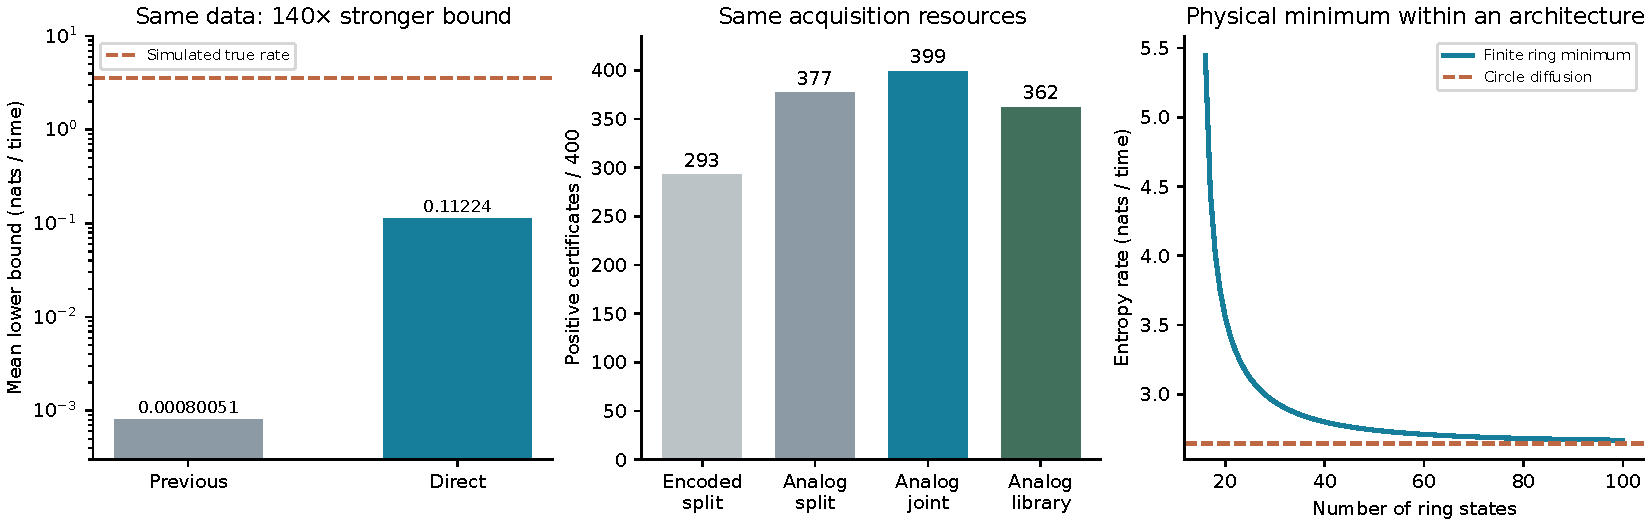
\includegraphics[width=\textwidth]{figures/attainability.pdf}
\caption{Distinct meanings of improvement. Left: the new physical bridge
strengthens a lower bound using the same frozen observations. Middle: joint
analog confidence increases detection at matched acquisition cost; selecting
from a library pays an explicit statistical penalty. Right: physically
realizable ring minima approach the known circle value inside a specified
architecture. All numerical panels describe mathematical models and simulated
records, not new laboratory measurements.}
\label{fig:pa-overview}
\end{figure}

For practical use, start with the acquisition contract in the joint analog
chapter and the executable \texttt{attainability\_tutorial.py}. The proofs,
negative controls, retained records and independent internal review then make
each assumption and comparison inspectable. The direct scalar inequality is
distinguished from the closest existing correlation-based inference results
in the final positioning section. Historical priority and empirical validation
remain open.

\chapter{Dissipation from a finite-lag correlation defect}
\label{ch:pa-spectral-dynamics}

A positive departure from a reversible correlation inequality contains more
information than a generic distance-to-equilibrium argument retains. The
operator identity below turns that departure directly into a lower bound on
stationary entropy production. The improvement is linear in a small positive
correlation defect; the previous comparison followed by Pinsker's inequality
was quadratic in its confidence gap. Both statements remain valid under their
respective contracts.

This is a theorem for a specified stochastic model class. It does not identify
the hidden generator, establish the exact minimum dissipation over all
compatible continuous-time models, or infer physical entropy from an arbitrary
oscillatory record. The distinction between ordinary and generalized time
reversal is essential.

\section{Population theorem and its operational assumptions}

Let $X_t$ be a stationary, time-homogeneous Markov process with invariant law
$\pi$ and transition semigroup $P_t$. Initially consider a finite irreducible
CTMC with positive stationary probabilities. Its physical time reversal must
be the \emph{ordinary reversal of the complete hidden state}, so that its
reverse generator is the $L^2(\pi)$ adjoint $Q^\dagger$. Define
\[
 \sigma=\sum_{x\ne y}\pi_x Q_{xy}
       \log\frac{\pi_xQ_{xy}}{\pi_yQ_{yx}}.
\]
The usual conventions give infinite entropy production for an unpaired
positive transition. The finite-entropy case is the informative one below.
Physical heat or power additionally requires a thermodynamic embedding; all
rates here are dimensionless entropy per unit physical time.

Let $f$ be a real bounded function with a valid range bound
$\sup f-\inf f\leq R$, $R>0$. This may be the conditional mean of a
noninvasive memoryless detector. Detector noise must be conditionally
independent between retained readings. Its range bound concerns the whole
admissible channel, not the largest and smallest values in a finite sample.
Set
\[
 C(t)=\langle f,P_t f\rangle_\pi,
 \qquad
 \Delta_s(t)=-s^2 C(0)+2sC(t)-C(2t),\quad t>0.
\]
The population identity allows any real $s$. Selecting $s$ from inference
data requires a simultaneous confidence argument or an independent pilot.

\begin{theorem}[Finite-lag dissipation bound]
\label{thm:pa-finite-lag}
Put $d=[\Delta_s(t)]_+$ and $u=4d/R^2$. Then $0\leq u\leq1$.
If $\sigma$ is finite, $u<1$ whenever $d>0$, and
\begin{equation}
 \boxed{\displaystyle
 \sigma\ \geq\ \frac{\Phi(u)}{t}\ \geq\
 \frac{8[\Delta_s(t)]_+}{R^2 t},
 \qquad
 \Phi(u)=2\sqrt{u}\,\operatorname{atanh}\sqrt{u}.}
 \label{eq:pa-direct-bound}
\end{equation}
Here $\Phi(0)=0$ and $\Phi(1)=+\infty$. The theorem requires no bound on
the number of hidden states or transition rates.
\end{theorem}

\begin{proof}
Write $P=P_t$, $H=(P+P^\dagger)/2$ and $B=(P-P^\dagger)/2$.
These are the self-adjoint and skew-adjoint parts of the transition operator,
not of the generator. In a real Hilbert space,
\begin{align}
 C(2t)&=\langle P^\dagger f,Pf\rangle_\pi
       =\|Hf\|_\pi^2-\|Bf\|_\pi^2,\\
 \Delta_s(t)&=\|Bf\|_\pi^2-\|(H-sI)f\|_\pi^2
              \leq\|Bf\|_\pi^2.
 \label{eq:pa-defect-identity}
\end{align}
In particular a reversible process, for which $B=0$, has no positive defect.

For each state $x$, let $v_x$ be the total variation between the probability
rows $P(x,\cdot)$ and $P^\dagger(x,\cdot)$. The bounded-expectation
inequality gives
\[
 |Bf(x)|\leq\frac{R}{2}v_x,
 \qquad u\leq\sum_x\pi_x v_x^2\leq1.
\]
Let $\mu(x,y)=\pi_xP(x,y)$ and $\mu^\leftarrow(x,y)=\mu(y,x)$ be
the forward and reverse stationary endpoint laws. Transposition exchanges the
two laws, so their relative entropies in opposite directions are equal. Since
both first marginals are $\pi$,
\begin{align}
 D(\mu\Vert\mu^\leftarrow)
 &=\frac12\sum_x\pi_x\bigl\{
       D(P_x\Vert P_x^\dagger)+D(P_x^\dagger\Vert P_x)\bigr\}\\
 &\geq\sum_x\pi_x\,2v_x\operatorname{atanh}v_x.
\end{align}
The last inequality is the established sharp Jeffreys--total-variation
inequality \cite{paSason2015}. The power series
\[
 \Phi(u)=2\sum_{k=1}^\infty\frac{u^k}{2k-1}
\]
shows that $\Phi$ is increasing and convex on $[0,1)$, with
$\Phi(u)\geq2u$. Jensen's inequality therefore gives
\[
 D(\mu\Vert\mu^\leftarrow)
 \geq\Phi\!\left(\sum_x\pi_xv_x^2\right)\geq\Phi(u).
\]
Finally, retaining only the endpoints cannot increase relative entropy.
The forward and ordinarily reversed stationary CTMC path laws over $[0,t]$
have relative entropy $t\sigma$. Consequently
$t\sigma\geq D(\mu\Vert\mu^\leftarrow)\geq\Phi(u)$.
\end{proof}

The elementary linear version follows already from conditional Pinsker and
the same identity. The nonlinear version retains the sharp symmetric
divergence ingredient. Neither version assumes that the observed scalar
record is itself Markovian: the semigroup acts on the full hidden state.

\section{What is sharp, and what remains a realization problem}

The endpoint bound is sharp over stationary discrete-time Markov kernels.
To see this, take a four-state cycle with uniform stationary law and
\[
 P_{i,i+1}=\frac{1+z}{2},\qquad
 P_{i,i-1}=\frac{1-z}{2},\qquad 0<z<1,
\]
with indices modulo four. For $f=(1,1,-1,-1)$ and $s=0$,
\[
 C_0=1,\quad C_1=0,\quad C_2=-z^2,\quad
 \Delta_0=z^2,\quad R=2.
\]
Every row has total variation $z$ from its reverse, and
\[
 D(\mu\Vert\mu^\leftarrow)
 =z\log\frac{1+z}{1-z}=\Phi(z^2).
\]
Thus equality holds throughout the endpoint argument.

This example does \emph{not} establish sharpness among finite CTMCs:
$\det P=-z^2<0$, whereas $\det e^{tQ}=e^{t\operatorname{tr}Q}>0$.
The sharp kernel cannot be the finite-time transition matrix of a finite
CTMC. The contraction from a full continuous path to its endpoints can lose
further information. Determining the best CTMC-compatible rate from a given
finite correlation record remains a separate physical realization problem.

For a nearest-neighbor ring with uniform stationary law and the cosine
detector, write its Fourier eigenvalue as $-\gamma+i\omega$. Then
\[
 C(t)=\tfrac12 e^{-\gamma t}\cos(\omega t),\qquad
 s=e^{-\gamma t}\cos(\omega t),\qquad
 \Delta_s(t)=\tfrac12e^{-2\gamma t}\sin^2(\omega t).
\]
The nonnegative residual in \eqref{eq:pa-defect-identity} vanishes for this
mode, but the subsequent information inequalities need not be saturated.
This avoids interpreting a convenient exact spectral example as a universal
minimum-dissipation model.

\section{Use with finite-confidence calibration}

Suppose an existing confidence construction returns $g\geq0$ such that,
on an event of probability at least $1-\alpha$,
\[
 2g\leq[\Delta_s(t)]_+.
\]
Both the same-state binary-twin construction and the bounded analog joint
construction provide such a gap. For the analog detector, writing
$f(x)=\mathbb E[Z\mid X=x]$ gives
\[
 B_{\rm obs}=\mathbb E Z^2\geq\mathbb E f(X)^2=C(0).
\]
The coefficient of the diagonal moment is $-s^2$, so its excess measurement
noise makes the contrast conservative. With
$q_0=(1+B_{\rm obs})/2$, $q_1=(1+C(t))/2$, $q_2=(1+C(2t))/2$,
\[
 a_s=(-s^2,2s,-1),\qquad b_s=-\frac{(1-s)^2}{2},
 \qquad 2(a_s\cdot q-b_s)\leq\Delta_s(t).
\]
Consequently the same confidence event yields
\begin{equation}
 \sigma\geq\frac{1}{t}\Phi\!\left(\frac{8g}{R^2}\right)
 \geq\frac{16g}{R^2t}.
 \label{eq:pa-statistical-direct}
\end{equation}
For a detector mean in $[-1,1]$, $R=2$ gives the particularly simple
lower bound $4g/t$. There is no new statistical failure allowance for replacing
the old physical implication by this stronger one. Taking a maximum with
another bound is justified without an extra penalty only when both follow
on the same already-covered event, or have separate simultaneous coverage.

The implementation returns exact rational bounds. For $0\leq u<1$ and
an integer $K\geq1$,
\[
 2\sum_{k=1}^K\frac{u^k}{2k-1}
 \leq\Phi(u)\leq
 2\sum_{k=1}^K\frac{u^k}{2k-1}
 +\frac{2u^{K+1}}{(2K+1)(1-u)}.
\]
The upper endpoint encloses the \emph{lower-bound formula}, not the actual
entropy production. If a confidence gap implies $u\geq1$, the API flags
incompatibility with finite entropy \emph{on the coverage event}; it retains
the valid linear inequality and does not silently clip $u$ or treat a possible
confidence failure as an empirical refutation of the model.

\section{Reanalysis of the frozen joint-calibration experiment}

The sixth-edition joint-calibration count archive contains 400 independent
simulated datasets in each of four declared cases. Its contrast, confidence
level, counts, and acquisition resources were fixed before those datasets
were generated. Recomputing the old certificates reproduces all saved rates
exactly. Applying \eqref{eq:pa-statistical-direct} then changes only the
mathematical physical bound, without collecting data or selecting a new
contrast.

\begin{center}
\begin{tabular}{lrrr}
Case & Positive datasets & Previous mean bound & New nonlinear mean bound\\
\hline
Driven ring & $399/400$ & $0.0008005133$ & $0.1122449304$\\
Equilibrium & $0/400$ & $0$ & $0$\\
High readout noise & $6/400$ & $0.0000002836$ & $0.0002243291$\\
Invalid calibration & $400/400$ & $0.0105740727$ & $0.4597513517$\\
\end{tabular}
\end{center}

The driven mean is $140.216$ times the former mean, while its actual model
entropy production is about $3.55736$. The new mean is about $3.16\%$ of
that value: the improved inference still leaves a substantial gap. Positive
detection counts are unchanged because the same positive confidence gap is
used. Each dataset still has 20,000 pair acquisitions, 40,000 endpoint
readouts and 24,000 units of declared evolution time; preparation and detector
overheads require their existing separate calibration.

The invalid-calibration row is a failure control, not a successful inference.
Changing the detector between calibration and science measurements violates
the shared-channel premise and produces false positive certificates even
for equilibrium. A stronger valid inequality cannot repair an invalid
measurement contract. The archived reanalysis is retrospective simulated-data
evidence, not new physical experimental validation.

\section{Vector observations and diffusion processes}

The same proof holds for a bounded detector map $F$ into a real Hilbert space,
with image diameter at most $R$, if
\[
 C(t)=\mathbb E\langle F(X_0),F(X_t)\rangle.
\]
For each row, the difference between the two vector expectations is total
variation times the difference of two barycenters of the detector image.
Its norm is at most $R v_x$, since taking the convex hull does not enlarge
diameter. The operator identity holds componentwise, or directly in the
corresponding Hilbert-valued $L^2$ space. All remaining inequalities are
unchanged. This proves a joint-diameter bound, rather than adding scalar
entropy lower bounds, an addition which would generally be invalid.

For example, replacing the cosine channel by
$F(\theta)=(\cos\theta,\sin\theta)$ doubles the ring correlation and
its defect while retaining diameter two. The linear population bound doubles;
the nonlinear one improves further. This is a changed observation channel,
whose full vector acquisition and readout costs must be recorded. It is not
additional information obtained by processing the original cosine alone.
For a noisy vector detector $Z$ confined to the unit ball,
$\mathbb E\|Z\|^2\geq\mathbb E\|\mathbb E(Z\mid X)\|^2$, and the
scores $(1+\|Z\|^2)/2$ and $(1+\langle Z_0,Z_t\rangle)/2$ have ranges
$[1/2,1]$ and $[0,1]$. This supplies the analogous joint-score construction;
the executable scalar benchmark does not claim a measured vector advantage.

The result also transfers to a stationary ordinary-even overdamped diffusion
whenever the forward and reversed path laws exist with
$D(\mathbb P_{[0,t]}\Vert\mathbb P^\leftarrow_{[0,t]})=t\sigma$.
For the smooth, compact, uniformly elliptic setting, or the separately
justified absolute-continuity setting of the diffusion chapter, the proof
uses the same transition-kernel identity and conditional divergences.
Here the reverse comparison is $Q^\dagger$, and its path divergence is
$t\sigma$, rather than the earlier reversible comparison's $t\sigma/4$.
Those constants belong to different comparisons and cannot be interchanged.

\section{Counterexamples that delimit the inference}

Stationarity cannot be replaced by a reversible generator alone. Take
$Q=\left(\begin{smallmatrix}-1&1\\1&-1\end{smallmatrix}\right)$,
$f=(1/2,1)$ and initialize the process in state zero. Its nonstationary
products obey $C(t)=3/8-e^{-2t}/8$, so
\[
 -C(0)+2C(t)-C(2t)=\tfrac18(1-e^{-2t})^2>0.
\]
The generator's stationary entropy production is zero. The positive record
defect therefore does not imply a positive stationary entropy rate without
the stationary-preparation assumption.

Likewise, observing an even physical quantity is insufficient to establish
ordinary time reversal for the hidden state. An equilibrium inertial
oscillator has an even position and odd velocity; its bounded position
readouts can have oscillatory correlations and a positive defect while its
physical entropy production is zero. Another explicit model is circle
drift--diffusion with the physical involution $\theta\mapsto-\theta$.
Its generator $Q=\omega\partial_\theta+D\partial_\theta^2$ obeys
$\Theta Q\Theta=Q^\dagger$ and is generalized reversible under that
involution. The even observable $\cos\theta$ has
$C(t)=e^{-Dt}\cos(\omega t)/2$; at $\omega t=\pi/2$ and $s=0$,
$\Delta_s=e^{-2Dt}/2>0$. Its ordinary-reversal mathematical entropy and
its generalized-reversal physical entropy are different quantities. The
theorem applies to the former unless ordinary full-state reversal has been
physically justified.

Finally, related spectral, cross-correlation and variance-sum-rule
dissipation bounds are established prior work. The specific contribution
tested here is the finite-lag scalar-defect implication, its sharp endpoint
envelope with explicit nonembedding caveat, and its integration with the
already-covered calibration record. The adjacent literature assessment
identifies the closest results and does not claim historical priority.

\chapter{Joint inference with one-reading analog calibration}
\label{ch:pa-joint-analog}

A bounded analog detector can supply its calibration coordinate with a single
reading. No unchanged-state twin is needed for the conservative construction
below. Combining that coordinate with the two dynamical scores gives a single
confidence bound. The direct semigroup dissipation inequality then converts
the same covered contrast into a substantially stronger physical certificate.
The statistical construction extends the joint-calibration and direct-analog
chapters; its ingredients remain the reversible quadratic moment inequality,
conditional Jensen, and Hoeffding concentration.

\section{The observable second moment has the useful inequality sign}
Let $Z\in[-1,1]$ be the output of a fixed noninvasive memoryless detector, with
conditional mean $f(x)=\mathbb E[Z\mid X=x]$. Use the stationary notation
\[
 A=\mathbb E_\pi f^2,\qquad B=\mathbb E_\pi Z^2,
 \qquad C_k=\langle f,P^k f\rangle_\pi,
 \qquad P=e^{\Delta Q}.
\]
Conditional detector noise at the two endpoints of a positive-lag pair is
independent. Consequently
\[
 B=A+\mathbb E_\pi\operatorname{Var}(Z\mid X)\geq A.
\]
\[
 W_0=\frac{1+Z^2}{2}\in[1/2,1],\qquad
 W_k=\frac{1+Z_0Z_{k\Delta}}2\in[0,1]\quad(k=1,2),
\]
and their means are $p_0=(1+B)/2$ and $p_k=(1+C_k)/2$.
Here $C_0=A$; the observable squared reading estimates $B$, not $A$.

\begin{proposition}[One-reading analog reversible support]
For fixed $0\leq s\leq1$, let $a_s=(-s^2,2s,-1)$ and
$b_s=-(1-s)^2/2$. Every reversible model satisfying this detector contract obeys
\begin{equation}
 a_s\cdot p-b_s
 =\frac{-s^2B+2sC_1-C_2}{2}
 =-\frac{\|(P-sI)f\|_\pi^2+s^2(B-A)}2\leq0.
 \label{eq:pa-analog-support}
\end{equation}
The support $b_s$ is sharp across the allowed detector class.
\end{proposition}
\begin{proof}
For reversible $Q$, the operator $P$ is self-adjoint, so
$\|(P-sI)f\|_\pi^2=C_2-2sC_1+s^2A$.
The additional conditional-variance term is nonnegative. The deterministic
zero-output detector attains equality for every $s$.
\end{proof}

The detector's noise costs population signal:
\[
 g_s^{\rm analog}=g_s^{\rm ideal\ twins}-\frac{s^2}{2}(B-A).
\]
Avoiding twins therefore does not guarantee better power. When the detector
noise dominates its state-dependent signal, the conservative square may erase
the violation entirely. For a state-independent fair detector with outputs
$\pm1$, $A=0$, $B=1$, and the analog gap is $-s^2/2$, even though its true
conditional mean contains no state information. This example also shows why
one cannot silently reinterpret a squared noisy reading as $A$.

\section{One confidence event, with every acquisition counted}
Take $n_0$ independent stationary single readings and $n_1,n_2$ independent
stationary pairs at the two lags. Let $\widehat p_k$ denote their score means.
For a fixed or independently piloted $s$, define
\begin{align}
 r_s&=\sqrt{\frac{\log(1/\alpha)}2
       \left(\frac{s^4}{4n_0}+\frac{4s^2}{n_1}+\frac1{n_2}\right)},
       \label{eq:pa-analog-radius}\\
 \underline g_s&=\left[
   -s^2\widehat p_0+2s\widehat p_1-\widehat p_2-b_s-r_s
   -\sum_{k=0}^2|a_{s,k}|(e_k+\delta_k)
 \right]_+.
 \label{eq:pa-analog-gap}
\end{align}
Here $e_k$ bounds numerical error in an empirical mean, and $\delta_k$ bounds
the conditional mean discrepancy from its ideal target given the entire past.
Independent stationary acquisitions have $\delta_k=0$. The conditional version
requires a valid external bound, not merely marginal stationarity. Hoeffding's
bound, or its conditional exponential-moment proof, gives the stated event
with failure at most $\alpha$. Independently established contract failure can
be added by a union bound. The API records these premises without verifying
them from the score summaries.

The factor $1/4$ in the first variance term is the square of the score's range
length $1/2$. It does not eliminate that term. For example, use a reversible
reset generator with stationary distribution $(1/2,1/4,1/4)$, detector values
$(0,1,-1)$, decay $1/2$, and $s=1/2$. Then $A=1/2$ and the ideal score means
are $(3/4,5/8,9/16)$, exactly on the support. One calibration reading is zero
with probability $1/2$, giving $\widehat p_0=1/2$. Even if the two dynamical
means were known exactly, treating that calibration reading as exact would
create a false gap $1/16$. Equation~\eqref{eq:pa-analog-radius} retains the
uncertainty and prevents this example from giving a positive certificate.

This design uses
\[
 N_{\rm acquisitions}=n_0+n_1+n_2,\qquad
 N_{\rm readouts}=n_0+2n_1+2n_2,\qquad
 T_{\rm evolution}=\Delta n_1+2\Delta n_2.
\]
Preparation, reset, sensor and calibration overhead must also be counted when
known. None is assigned zero physical energy here. The exact square-summary
helper rounds the score with a declared numerical radius; it bounds the
rounding error of stored digital readings, not unknown sensor calibration
error.

\section{A direct physical conversion on the same event}
Under the stationary even-variable Markov assumptions of the direct spectral
dissipation theorem, the detector mean has range at most two and
\[
 -s^2B+2sC_1-C_2\leq -s^2A+2sC_1-C_2.
\]
Thus the covered gap in~\eqref{eq:pa-analog-gap} supplies
\begin{equation}
 \sigma\geq\frac{4\underline g_s}{\Delta},\qquad
 \sigma\geq\frac{\phi(2\underline g_s)}{\Delta},\qquad
 \phi(u)=2\sqrt u\,\operatorname{atanh}\sqrt u,
 \quad 0\leq u<1.
 \label{eq:pa-analog-direct-bridge}
\end{equation}
The implementation encloses $\phi$ with a positive rational series. The
interval is an enclosure of this lower-bound formula, not an interval for
the true entropy production. An incompatible normalized defect is flagged
on the coverage event; it is not silently clipped or presented as empirical
falsification.

For comparison, the earlier additive-reversible record argument gives
\begin{equation}
 \sigma\geq
 \frac{8\underline g_s^2}{(2s\sqrt\Delta+\sqrt{2\Delta})^2}.
 \label{eq:pa-analog-old-bridge}
\end{equation}
The zero-lag squared-reading law is unchanged by additive reversibilization
because the stationary law and detector channel are unchanged. It therefore
contributes sampling uncertainty and apparatus expenditure but no comparison
divergence in~\eqref{eq:pa-analog-old-bridge}. The stronger direct argument
uses the semigroup identity and forward/reverse comparison instead. Both
physical conversions reuse the same confidence event; they spend no additional
$\alpha$. Different choices of $s$ still require independent selection or a
simultaneously valid procedure.

\section{Frozen comparison on the same analog data}
The benchmark fixes all models, parameters, counts, rules and random seed
before drawing its 1,600 held-out synthetic datasets. Each of four cases has
400 independent datasets. A 20-state circulant CTMC is observed through a
cosine detector rounded to denominator 4096. Each dataset contains 4,000
single-reading calibration acquisitions and 3,000 pairs at each of lags
$1/10$ and $1/5$. Every compared method therefore receives the same
10,000 acquisitions, 16,000 detector readings and 900 declared units of
evolution time.
These comparisons match acquisition resources. Their analysis-computation
time and energy are unmeasured and are not asserted equal.

The base contrast has $s=1/2$, reproducing the earlier difference of positive-lag
scores. A second contrast fixes $s=3/4$ before production; ``tuned'' refers to
this predetermined design, not a fit to the held-out records. The split methods
call the sixth edition's actual analog calibration and score APIs, with
$\alpha/2=1/40$ for each stage. The joint methods use $\alpha=1/20$. Virtual
coin methods retain a draw from $\operatorname{Bernoulli}(W_k)$ for each same
analog pair. The calibration singles are common to every method.

\begin{center}
\begin{tabular}{lrrr}
\toprule
Method & Driven & Equilibrium & Noisy driven\\
\midrule
Joint analog, $s=1/2$ &399/400&0/400&0/400\\
Joint analog, $s=3/4$ &399/400&0/400&0/400\\
Joint coin, $s=3/4$ &361/400&1/400&0/400\\
Split analog, $s=1/2$ &377/400&0/400&0/400\\
Split analog, $s=3/4$ &379/400&0/400&0/400\\
Split coin, $s=1/2$ &293/400&0/400&0/400\\
\bottomrule
\end{tabular}
\end{center}

The driven rates are 20 forward and 1 backward; equilibrium rates are both
$21/2$. The noisy detector outputs half the rounded cosine plus an independent
fair noise of amplitude $1/2$. Its squared-reading calibration is too
conservative here, and every method returns zero in all 400 datasets.
An exact population audit explains this failure. For $B>0$, completing the
square gives
\[
 \sup_{s\in\mathbb R}g_s^{\rm analog}
 =\frac12\left(\frac{C_1^2}{B}-C_2\right).
\]
Rational uniformization of this fixed noisy ring encloses both correlations
and certifies that the right side is below $-0.007$. Its numerical value is
approximately $-0.00789686$. The entire two-lag quadratic family therefore
lacks a positive population gap here. More samples at these same settings
cannot repair this obstruction; different lags, additional noise calibration
or different observables remain possible. This retrospective exact audit does
not change the frozen inference design or any reported decisions.
The single equilibrium rejection by the joint coin method is reported rather
than removed; the methods have individual 5\% failure allowances.

Keeping the older quadratic physical conversion isolates the statistical
improvement. At $s=1/2$, the driven mean lower bound rises from $0.00145847$
for split analog to $0.00351542$ for joint analog. At $s=3/4$, it rises from
$0.00164098$ to $0.00494257$. Applying the new direct bridge to that same
joint $s=3/4$ event gives a mean linear bound $0.870376$ and a mean nonlinear
bound $0.884824$: the latter is about 179 times the older quadratic mean.
The simulated model's actual rate is $56.9189$, so even the improved mean is
only 1.55\% of the microscopic value. This large remaining gap is explicit.

The virtual coin's greater variance can increase the average of a clipped
quadratic lower bound even while reducing detection probability. Indeed its
joint $s=3/4$ quadratic mean is $0.00639217$, above the analog value, despite
361 rather than 399 detections. This is why an average positive-part bound
alone does not establish estimator quality or universal statistical dominance.
The matched table reports detection counts, means, medians and Monte Carlo
intervals in the accompanying results.

\section{A detector change remains a physical failure}
The fourth case uses an equilibrium ring with rates 70 in both directions,
but replaces the calibration detector by zero gain while retaining the cosine
science detector. This deliberately violates the common-channel contract.
Both joint analog methods and both split analog methods falsely return positive
values in all 400 datasets. The split coin returns 395 positives and the joint
coin 400. Correcting the zero-lag conditional-mean discrepancy by the general
bound $\delta_0=1/2$ makes the reported repair return zero in all datasets.
This repair is deliberately conservative; obtaining a useful smaller bound
requires actual detector calibration.

The archive retains every dataset's exact integer sufficient statistics and
the first raw analog bank in each case. Rational score means can be replayed
without drawing new coins or trajectories. The six methods are separate
predeclared analyses; their unadjusted maximum is not advertised as a 95\%
certificate. These are reproducible simulations, not new measured physical
data or a universal noise-removal procedure. Physical use requires stationary
preparation, the appropriate reversal convention, detector independence and
memory control, time calibration, and a justified thermodynamic embedding for
conversion from entropy rate to dissipated power.

\chapter{Repairing a noise obstruction by changing the measurement lag}
\label{ch:pa-retiming}

The noisy example in Chapter~\ref{ch:pa-joint-analog} cannot produce a
positive population gap anywhere in its chosen two-lag quadratic family.
That obstruction concerns a specific set of observation times. Retaining the
same detector and changing those times exposes a negative correlation, which
does admit a dissipation certificate. The new experiment below recovers
386 positive certificates in 400 fresh noisy datasets, compared with zero
for either former fixed contrast, at the same declared evolution time and
with substantially fewer detector readings.

This is a complete example of the research loop: certify why the present
protocol fails, change an identifiable feature of physical access, and test
the resulting prediction on new data. Negative-correlation constraints and
the use of temporal correlations to study irreversibility have established
antecedents~\cite{vlAldousFill2002,ciVSR2024,ciVSRProofs2024}. The contribution
here is the explicit repair, its direct finite-data dissipation bound and its
frozen comparison. It is not a claim that useful timing is new or that every
unknown system has a similarly favorable lag.

\section{One observed lag is sufficient}
Assume the stationary homogeneous Markov and ordinary even-variable reversal
conditions of Theorem~\ref{thm:pa-finite-lag}. Let $Z\in[-1,1]$ be the same
noninvasive memoryless analog detector, with conditional mean $f$ and
independent endpoint noise. Write
\[
 C(\tau)=\mathbb E[Z_0Z_\tau]=\langle f,e^{\tau Q}f\rangle_\pi.
\]
Under a reversible explanation,
\[
 C(\tau)=\|e^{\tau Q/2}f\|_\pi^2\geq0.
\]
This condition includes a nonzero detector mean; no mean subtraction or
zero-lag second-moment estimate is needed for this particular test.

\begin{corollary}[Negative-correlation dissipation certificate]
Set $t=\tau/2$ and $s=0$ in the direct finite-lag theorem. If an already
covered lower bound $g\geq0$ obeys $2g\leq[-C(\tau)]_+$, then
\begin{equation}
 \sigma\geq\frac{2\Phi(2g)}{\tau}\geq\frac{8g}{\tau},\qquad
 \Phi(u)=2\sqrt u\,\operatorname{atanh}\sqrt u,
 \quad 0\leq u<1.
 \label{eq:pa-retiming-bridge}
\end{equation}
The conclusion concerns the same physical model and confidence event.
\end{corollary}
\begin{proof}
The semigroup defect becomes
$-s^2C(0)+2sC(t)-C(2t)=-C(\tau)$.
The two unused coordinates have zero coefficients, so they need not be
measured. The detector mean has range at most two. Substituting $t=\tau/2$
and normalized covered defect $2g$ into the direct theorem gives the result.
\end{proof}

The hidden semigroup identity uses $\tau/2$, but the instrument does not
perform a half-lag measurement. It records only the two endpoints separated
by $\tau$. There are no dedicated zero-lag calibration acquisitions. Bounds
on the detector, its channel stability and memory, the clock and stationary
preparation remain physical calibration requirements.

For $n$ independent stationary pairs, let
$W_i=(1+Z_{i,0}Z_{i,\tau})/2\in[0,1]$. At failure probability $\alpha$,
\begin{equation}
 g_n=\left[\frac12-\overline W
   -\sqrt{\frac{\log(1/\alpha)}{2n}}-e-\delta\right]_+
 \label{eq:pa-retiming-confidence}
\end{equation}
is valid. The quantity $e$ bounds numerical mean error, and $\delta$ bounds
a declared conditional mean discrepancy given the complete preceding record.
The independent stationary-pair design has $\delta=0$. This is Hoeffding's
one-sided bound; it does not assume that an analog score is a Bernoulli
count. The implementation accepts exact product sums, propagates the declared
errors, and applies the same rational enclosure of $\Phi$ as the preceding
chapter. A lag chosen on these same inference records requires a separate
selection correction.

\section{An exact reason to move the lag}
The earlier ring has 20 states, clockwise rate 20 and counterclockwise rate 1.
For an ideal cosine detector, its fundamental-mode correlation has the form
\[
 C(\tau)=A e^{-\gamma\tau}\cos(\omega\tau),\qquad
 \gamma=21\bigl(1-\cos(2\pi/20)\bigr),\quad
 \omega=19\sin(2\pi/20).
\]
The implemented detector is rounded to denominator 4096; the noisy channel
adds an independent fair noise of amplitude $1/2$ to half that cosine.
The exact audit therefore uses the actual rational detector and generator,
not the ideal single-mode approximation.

At the former lags $0.1$ and $0.2$, completing the square and exact
uniformization showed that the greatest analog quadratic gap over every real
$s$ is below $-0.007$. At the newly fixed lag $\tau=0.5$, exact uniformization
instead encloses
\[
 C(0.5)\simeq-0.0732037920< -0.07.
\]
Its population linear dissipation bound is approximately $0.585630$; the
nonlinear bound is $0.600583$. Both remain far below the actual microscopic
rate $19\log20\simeq56.9189$.

The rational calculation expands $e^{\tau Q}$ by uniformization with rate 21.
Each discrete-step correlation has absolute value at most $A$, by stationary
Markov contraction in $L^2(\pi)$. A geometric bound on the positive exponential
tail therefore encloses the omitted correlation contribution, including either
sign. Eighty terms give the reported rigorous interval. An independent
100-digit Fourier calculation checks that interval. This calculation and the
choice of the new lag use the known model after the earlier failed protocol;
the subsequent evaluation uses a new random seed and new held-out records.

\section{Fresh evaluation with equal evolution time}
Before generating the new evaluation bank, the design fixes
$\tau=1/2$, $n=1800$ and $\alpha=1/20$. The new method uses 1,800 stationary
pair preparations, 3,600 detector readings and 900 units of evolution time.
The comparison retains both former fixed values $s=1/2$ and $s=3/4$, each
using the actual joint-analog API and its stronger direct dissipation bridge.
Those methods receive fresh banks of 4,000 stationary single readings and
3,000 pairs at each of lags $0.1$ and $0.2$: 10,000 acquisitions, 16,000
readings and the same 900 units of evolution time.

Thus the retimed design uses 22.5\% as many readings, a factor $40/9$
reduction. Its preparation count also changes. Preparation, reset, detector
operation and processing overhead are unmeasured and are not assigned zero.
The comparison matches declared evolution time; it does not claim equal
total wall time, equal processing energy or a calibrated joule saving.

Four cases each receive 400 new datasets. The driven rates are 20 and 1;
the equilibrium rates are $21/2$ in each direction. Both clean and noisy
versions use the same channels defined above.
\begin{center}
\begin{tabular}{lrrr}
\toprule
Case & Old $s=1/2$ & Old $s=3/4$ & Retimed\\
\midrule
Driven &400/400&400/400&400/400\\
Equilibrium &0/400&0/400&0/400\\
Noisy driven &0/400&0/400&386/400\\
Noisy equilibrium &0/400&0/400&0/400\\
\bottomrule
\end{tabular}
\end{center}
The noisy detection fraction is 96.5\%, with a nominal Wilson 95\% Monte
Carlo interval of 94.21--97.90\%. Its mean nonlinear lower bound is
$0.124947$, only 0.2195\% of the actual rate. Retiming restores a usable
certificate in this example; it does not reconstruct the microscopic
dissipation accurately. For the clean driven case, the mean bound is
$2.05450$, compared with $0.621640$ and $0.900411$ for the two earlier fixed
designs. None of the 1,600 datasets produces a bound above its model's true
rate. That simulation observation is additional checking, not a replacement
for the confidence proof.

All three methods have individual 95\% certificates. Their unadjusted maximum
is not advertised as another 95\% certificate. The archive preserves every
dataset's exact sufficient statistics and the first raw bank of each case.
Independent code reconstructs every reported rate and checks the raw-bank
summaries, physical counts and population intervals.

\section{What this repair does and does not identify}
The timing change avoids the conservative $B-A$ calibration penalty because
the zero-lag coefficient is zero. Independent detector noise still reduces
the conditional mean signal and hence the accessible correlation. It does
not vanish from the experiment, and many driven systems or available lag
ranges may have no statistically useful negative correlation.

The ordinary-reversal and detector assumptions also remain necessary. An
equilibrium one-state target coupled to an unobserved driven sensor ring can
produce exactly the same recorded law as the noisy driven example. The full
target-plus-sensor system dissipates, while the target alone need not.
Assigning the inferred lower bound to the target requires excluding such
sensor memory or including it in the physical system being bounded.
Equilibrium systems with odd hidden variables, such as inertial dynamics,
likewise require the correct reversal operation and a separate argument.

The result establishes a concrete change in experimental access: one protocol
family provably has no positive population gap, while a redesigned timing
choice provides a finite-data dissipation certificate with fewer readings at
the same evolution budget. It is a model-assisted, reproducible repair under
stated assumptions, rather than a universal rule for selecting lags without
prior information about a system.

\chapter{Choosing a contrast from the observations}
\label{pa:design}
The direct bound needs a correlation contrast parameter $s$. A model can suggest
one, but requiring the correct hidden rates would undermine its practical use.
A finite predeclared library provides a simple alternative with explicit coverage.
This is an application of simultaneous confidence bounds, not a new statistical
principle.

Let $\mathcal S\subset[0,1]$ contain $M$ distinct rational values chosen before
collecting the inference records (an independent pilot is also allowed).
For each $s$, compute the joint analog lower gap $g_s$ with statistical failure
budget $\alpha/M$. The same calibration and pair records can be reused in every
contrast. The union bound gives
\[
 \Pr\{\text{all }g_s\leq\tfrac12[\Delta_s]_+\}\geq1-\alpha.
\]
Thus selecting the largest nonnegative gap after observing the data is valid:
\[
 \sigma\geq \frac{4}{t}\max_{s\in\mathcal S}g_s
\]
for a detector conditional mean of range at most two and the physical contract
of the direct semigroup theorem. The nonlinear bridge may likewise be applied
to this selected gap. An external calibration-contract failure $\eta$ is added
once, giving total failure at most $\alpha+\eta$. Independence between candidate
estimates is unnecessary. Acquisition costs count the shared records once.

The price is a larger confidence radius, with $\log(M/\alpha)$ in place of
$\log(1/\alpha)$. A correctly chosen fixed contrast can outperform the library.
A library picked or enlarged using these inference data does not satisfy the
proof; it requires a new coverage argument. Likewise, reporting the maximum of
several methods that each individually use all of $\alpha$ is invalid without
simultaneous coverage.

The executable \texttt{certify\_library} function removes duplicate parameters,
allocates the error budget, retains the individual certificates, and returns the
selected contrast and its physical bound. A frozen library of seventeen values
$\{0,1/16,\ldots,1\}$ is evaluated on the same records as the joint analog study.
The full result is retained in \texttt{attainability/results/design.json}; it
reports the selection penalty and comparisons even where a fixed contrast wins.

On the driven analog benchmark, the predeclared library detects $362/400$,
compared with $399/400$ for each of the fixed $s=1/2$ and $s=3/4$ methods.
Its mean linear rate lower bound is $0.346861$, versus $0.600275$ and
$0.870376$ for those fixed contrasts. The equilibrium and strong-noise controls
both give $0/400$; the invalid detector-calibration control gives $400/400$
false positives and remains invalid. These results exhibit the cost of
protecting selection from a larger library. They do not justify replacing a
well-supported fixed design by a library in every experiment.

\chapter{Physical realizations and sampling limits}
\section{A physical minimum in a declared architecture}
\label{sec:pa-physical-minimum}

An upper bound on a relaxed record divergence is not a realizable upper bound
on the least dissipation compatible with a measurement. This section gives
an explicit physical construction and an exact optimization within one
architecture. The architecture assumption is substantial: translation-invariant
Markov dynamics on a ring, with the first Fourier mode observed. It is not
inferred merely from two measured correlations.

Let $n\geq3$ and let $k_j\geq0$ be the rate of the displacement
$x\mapsto x+j\pmod n$. Assume the displacement support is irreducible.
The stationary distribution is uniform. Write the first Fourier eigenvalue as
$-\gamma+i\omega$, where $\gamma>0$, so that
\begin{align}
 \gamma&=\sum_{j=1}^{n-1}k_j\{1-\cos(2\pi j/n)\},\\
 \omega&=\sum_{j=1}^{n-1}k_j\sin(2\pi j/n),\\
 \sigma&=\sum_{j=1}^{\lfloor(n-1)/2\rfloor}
       (k_j-k_{n-j})\log(k_j/k_{n-j}).
 \label{eq:pa-circulant-epr}
\end{align}
Terms with both rates zero contribute zero; a positive rate with zero reverse
rate contributes infinite entropy production. A self-inverse displacement
$j=n/2$ contributes no entropy. Entropy is dimensionless per unit time;
converting it to physical power requires the thermodynamic embedding.

The Fourier formulas, the general delocalized-mode inequality
$\sigma\geq\omega^2/\gamma$, and its saturation by circle drift--diffusion
are established results, discussed explicitly by Gu~\cite{rfGu2026}.
The finite-$n$ minimization below supplies a more restrictive, architecture-specific
answer. No historical-priority claim is made.

\paragraph{Theorem: finite-size circulant minimum.}
Fix $n,\gamma,\omega$. A finite-entropy circulant realization exists if and
only if
\begin{equation}
 \frac{|\omega|}{\gamma}<\cot(\pi/n).
 \label{eq:pa-circulant-feasible}
\end{equation}
Within that class the minimum is
\begin{equation}
 \boxed{\quad
 \sigma_n^{\min}(\gamma,\omega)
 =\frac{2\omega}{\sin(2\pi/n)}
   \operatorname{artanh}\!\left(
       \frac{\omega}{\gamma}\tan(\pi/n)\right).
 \quad}
 \label{eq:pa-circulant-min}
\end{equation}
The expression is even in $\omega$ and is zero at $\omega=0$. The minimizer
uses only the two nearest-neighbor displacements, with rates
\begin{equation}
 k_{\pm}=\frac12\left\{
 \frac{\gamma}{1-\cos(2\pi/n)}
 \mathbin{\pm}\frac{\omega}{\sin(2\pi/n)}\right\}.
 \label{eq:pa-circulant-rates}
\end{equation}
At equality in \eqref{eq:pa-circulant-feasible}, a one-way ring is possible
but has infinite ordinary-reversal entropy production. Above the boundary
there is no such circulant realization, even with infinite entropy.

\paragraph{Proof.}
Pair the displacements with angle $\theta_j=2\pi j/n\in(0,\pi)$.
Set $x_j=\tan(\theta_j/2)$, traffic $s_j=k_j+k_{n-j}$ and
current $d_j=k_j-k_{n-j}$. A nonzero pair contributes
\[
 \gamma_j=s_j(1-\cos\theta_j),\qquad
 \omega_j=d_j\sin\theta_j,\qquad
 \sigma_j=2d_j\operatorname{artanh}(d_j/s_j).
\]
For $u_j=\omega_j/\gamma_j$ this is
\[
 \sigma_j=\gamma_j F_{x_j}(u_j),\qquad
 F_x(u)=\frac{u(1+x^2)}{x}\operatorname{artanh}(xu),
 \qquad |xu|<1.
\]
The function is even in $u$, convex because
$F_x''(u)=2(1+x^2)/(1-x^2u^2)^2$, and nondecreasing in $x$ at fixed $u$.
For the last assertion, $\operatorname{artanh}(xu)/x$ is nondecreasing
for $u\geq0$, as follows from its positive power series; evenness handles
$u<0$. Since $x_j\geq x_*=\tan(\pi/n)$,
$F_{x_j}(u_j)\geq F_{x_*}(u_j)$. An antipodal displacement, when present,
adds damping with $u_j=0$ and zero entropy and can be included as another
weight. Jensen's inequality with weights $\gamma_j/\gamma$ gives
\[
 \sigma\geq\sum_j\gamma_j F_{x_*}(u_j)
 \geq\gamma F_{x_*}(\omega/\gamma),
\]
which is \eqref{eq:pa-circulant-min}. If a reverse rate vanishes the same
inequality holds with infinite left side. Also,
$|\omega_j|/\gamma_j\leq1/x_j\leq1/x_*$, strictly below the last
boundary for a finite-entropy nonzero oscillation. This proves necessity
of \eqref{eq:pa-circulant-feasible}. The positive rates
\eqref{eq:pa-circulant-rates} prove sufficiency and attain equality.
\hfill$\square$

For fixed nonzero $\omega$, the minimum decreases strictly as feasible $n$
increases, and
\begin{equation}
 \sigma_n^{\min}>\frac{\omega^2}{\gamma},\qquad
 \lim_{n\to\infty}\sigma_n^{\min}=\frac{\omega^2}{\gamma}.
 \label{eq:pa-circulant-limit}
\end{equation}
This follows from the same monotonicity of $F_x$ and $x=\tan(\pi/n)\downarrow0$.
Equivalently,
\[
 \frac{\sigma_n^{\min}}{\omega^2/\gamma}
 =\sec^2(\pi/n)\,
   \frac{\operatorname{artanh}(r_n)}{r_n},\qquad
 r_n=(\omega/\gamma)\tan(\pi/n).
\]
The finite-size overhead is physical, not a sampling-confidence penalty.

\paragraph{A complete correlation law with explicit realizations.}
For $0<A\leq1/2$, the bounded detector
$f(x)=\sqrt{2A}\cos(2\pi x/n)$ has
\begin{equation}
 C(t)=\mathbb E[f(X_0)f(X_t)]
     =A e^{-\gamma t}\cos(\omega t).
 \label{eq:pa-mode-correlation}
\end{equation}
Every ring constructed above realizes this same law for all $t\geq0$.
The circle diffusion
\[
 d\phi_t=\omega\,dt+\sqrt{2\gamma}\,dW_t\pmod{2\pi},\qquad
 f(\phi)=\sqrt{2A}\cos\phi
\]
has uniform stationary distribution, exactly the same correlation, and
$\sigma=\omega^2/\gamma$. This is an attainable physical value, unlike
an upper bound on a record-divergence relaxation. It provides an upper
bound on the \emph{infimum} of entropy among all compatible models in
any larger class containing this diffusion. It is not an upper bound on
the entropy of the unknown system. In the union of circulant finite-state
architectures, it is an infimum approached by finite rings.

For the earlier calibrated example $C(0)=1/2$, $C(1)=0.38$ and
$C(2)=0.18$, impose the single-mode model and write
$z=C(1)/A$, $w=C(2)/A$. Then
\[
 e^{-2\gamma}=2z^2-w=497/625,
 \quad \gamma=0.1145808118\ldots,
 \quad |\omega|_{\rm principal}=0.5504934894\ldots.
\]
The smallest feasible ring has $n=16$. Selected exact-form physical
minima, evaluated numerically, are
\begin{center}
\begin{tabular}{r|rrrrr|r}
$n$&16&20&40&100&1000&circle\\\hline
$\sigma_n^{\min}$&5.44695&3.55736&2.80013&2.66781&2.64502&2.64480
\end{tabular}
\end{center}
These numbers sharpen the declared ring problem, not the unrestricted
inverse problem. A hidden model outside this architecture can have the
same measured moments. Eigenvalue-only entropy bounds require particular
care outside the delocalized class; known counterexamples preclude replacing
this declaration with a universal claim~\cite{rfShiraishi2026}.

\paragraph{An explicit failure outside the architecture.}
Even the complete scalar correlation function does not by itself justify the
circulant minimum. Take a four-state nearest-neighbor ring with damping
$\gamma-\kappa$ and frequency $\omega$, where
$0<\kappa<\gamma-|\omega|$. Add a fifth state, called the hub.
From every ring state jump to the hub at rate $\kappa$; from the hub jump
to each ring state at rate $\beta/4$, where
$\beta=A\kappa/(1-A)$ and $0<A<1$. The stationary masses are
$\pi_i=A/4$ on the ring and $\pi_\mathrm{hub}=1-A$.
The hub edges obey detailed balance. The detector is
$f=(1,1,-1,-1,0)$, so $\mathbb E f=0$ and $\mathbb E f^2=A$.
The ring Fourier subspace has zero hub component and its damping increases
by $\kappa$, giving exactly
\[
 C(t)=A e^{-\gamma t}\cos(\omega t),\qquad
 \sigma=2A\omega\operatorname{artanh}\!\left(
                       \frac{\omega}{\gamma-\kappa}\right).
\]
The chain is irreducible and every nonzero edge has a positive reverse.
At $A=0.1$, $\gamma=1$, $\omega=0.5$, $\kappa=0.01$, the entropy is
$0.0556063004\ldots$, below the circle value $0.25$, despite identical
calibration and identical scalar covariance at every lag. Direct generator
calculations reproduce both values. Thus a circle construction provides a
compatible physical upper bound on the infimum; it does not prove the
unrestricted infimum equals that construction. The detector law beyond
second-order correlations may distinguish these architectures.

\section{Sampling can hide arbitrarily large physical dissipation}
\label{sec:pa-entropy-aliasing}

The same realizable example exposes a second limitation. Even full spatial
resolution at discrete times need not bound physical dissipation. This is a
thermodynamic consequence of ordinary sampling aliasing, closely related to
continuous-time system aliasing~\cite{paYue2021}.

\paragraph{Exact grid aliasing.}
Fix $\gamma>0$ and a sampling interval $\Delta>0$. The circle transition
kernel at time $\Delta$ depends on $\omega$ only through
$\omega\Delta\pmod{2\pi}$. Therefore every finite or infinite
stationary record sampled on that grid has exactly the same probability
law under
\begin{equation}
 \omega_k=\omega+2\pi k/\Delta,\qquad k\in\mathbb Z.
 \label{eq:pa-frequency-alias}
\end{equation}
This statement holds even if the full circle state is read at each instant.
Any detector or subsequent processing retains the equivalence. Yet
$\sigma_k=\omega_k^2/\gamma\to\infty$. Thus the known two-parameter
architecture and arbitrarily many grid records do not supply a finite
upper bound on dissipation without an additional frequency restriction or
access to intervening motion.

For the scalar covariance, $C(0),C(\Delta),C(2\Delta)$ identify
$\gamma$ and the principal value
\[
 \omega_0=\Delta^{-1}\arccos\!\left[
 \frac{C(\Delta)/A}{\sqrt{2(C(\Delta)/A)^2-C(2\Delta)/A}}\right]
\]
when the specified single-mode model is feasible. The frequencies
$\pm\omega_0+2\pi k/\Delta$ remain possible. Their smallest
circle entropy is $\omega_0^2/\gamma$; the supremum is infinite.
These conclusions concern the single-mode class and exact moments.

\paragraph{Exact identification need not give a stable entropy upper bound.}
If $\gamma$ and $A$ are known, three positive lags with pairwise irrational
ratios determine $|\omega|$ from exact cosine correlations. Indeed,
$\cos(\omega' t_j)=\cos(\omega t_j)$ implies
$\omega't_j=s_j\omega t_j+2\pi k_j$, with $s_j\in\{-1,1\}$.
Among three signs, two agree. An irrational ratio between the associated
lags forces both integers to vanish, and hence $\omega'=\omega$ or
$\omega'=-\omega$. Two such lags do not always suffice: at
$t_1=1,t_2=\sqrt2$, the distinct positive frequencies
$\pi(\sqrt2-1)$ and $\pi(\sqrt2+1)$ give identical cosines.

Exact uniqueness does not survive as a finite-precision upper bound.
Fix a finite menu of positive observation gaps, a fixed finite number of
intervals, and $\gamma>0$. For any reference $\omega$, there is a sequence
$|\omega_k|\to\infty$ whose entire sampled-state record distributions
converge in total variation to the reference distribution. This includes
adaptive choices from the finite gap menu with a bounded number of steps.

To prove the statement, write the gaps as $t_1,\ldots,t_m$ and use
simultaneous Diophantine approximation to choose arbitrarily large integers
$q$ such that the distances from $q t_j/t_1$ to integers approach zero.
If an exact common period exists, its multiples give the conclusion
immediately; otherwise the approximating denominators are unbounded.
Set $\omega_k-\omega=2\pi q/t_1$. All the wrapped phase shifts then
approach zero. For a gap $t$, let $\delta_t$ be its phase shift reduced to
$[-\pi,\pi]$. Comparing unwrapped normal increments and then wrapping gives
\begin{equation}
 \operatorname{TV}(K_\omega^t,K_{\omega_k}^t)
 \leq 2\Phi\!\left(\frac{|\delta_t|}{2\sqrt{2\gamma t}}\right)-1
 \leq\frac{|\delta_t|}{2\sqrt{\pi\gamma t}},
 \label{eq:pa-phase-tv}
\end{equation}
uniformly in the starting state. Sequential coupling bounds complete-record
TV by the sum of these transition bounds, or by the number of steps times
the largest menu bound. Independent replication multiplies the sum bound
by the number of records. Stopping and further detector processing cannot
increase it. Meanwhile $\omega_k^2/\gamma$ diverges.

Consequently every positive-TV neighborhood of the accessible law contains
models with unbounded entropy. More statistically, any upper procedure $U$
with uniform coverage $\Pr_\omega\{U\geq\omega^2/\gamma\}\geq1-\alpha$
for this experiment must satisfy
\begin{equation}
 \Pr_\omega\{U=+\infty\}\geq1-\alpha
 \quad\hbox{at every reference }\omega.
 \label{eq:pa-alias-upper-no-go}
\end{equation}
For any finite $M$, choose near-aliases with entropy exceeding $M$ and
record TV tending to zero. Uniform coverage then implies
$\Pr_\omega\{U\geq M\}\geq1-\alpha$; take $M\to\infty$.
This statement assumes a fixed finite gap menu and bounded experiment.
It does not address a continuously distributed random timing design whose
exact realized times are retained, an unbounded observation horizon, or a
separately calibrated frequency cap. Those changes alter access.

The implementation illustrates the near-alias mechanism constructively.
At gaps $1$ and $\sqrt2$, Pell solutions $p^2-2q^2=1$ give shifts
$2\pi q$, with second-gap phase error
$2\pi/(p+\sqrt2q)$. For $\gamma=1$, reference $\omega=1/2$, and
$(p,q)=(665857,470832)$, the alternative entropy is
$8.751688\times10^{12}$ while the two-interval full-state record TV
is at most $1.119197\times10^{-6}$. This is a mathematical model
calculation, not a physically achievable drive-rate claim. A calibrated
bandwidth excludes such alternatives; absent that calibration the model
allows them.

\paragraph{Reproduction and limits.}
\texttt{physical\_minimum.py} reconstructs generators, compares matrix
exponentials with \eqref{eq:pa-mode-correlation}, checks the inequality on
1,000 seeded nonlocal circulant generators, and saves the physical and
aliasing examples. Fourteen producer tests cover realization, nonlocal
jumps, equilibrium, one-way limits, invalid inputs, continuum convergence,
and exact and near aliasing. Floating-point evaluation is not advertised
as an interval certificate; the proofs establish the mathematical claims.
No new measured-data entropy estimate, universal physical minimum, or
historical priority follows from these calculations.

\chapter{What a reversible signal can require of its hidden dynamics}
\label{og:entry}

A recorded signal can have exactly the same law when played backwards and
still require positive dissipation from every admissible hidden model.
There is no contradiction: the recorded law and the physical class of its
possible generators supply different constraints. This chapter develops that
distinction for stationary, smooth, ordinary-reversal overdamped diffusions.
It does not extend the conclusion to arbitrary physical realizations.

The earlier correlation certificates give lower bounds without reconstructing
hidden dynamics. Their remaining gap raises a physical question: can any
admissible system actually attain the inferred minimum? The present layer
answers that question for a family of observed processes while allowing any
finite hidden dimension. It also identifies the extra access needed for this
answer. A covariance function alone is insufficient. Local fluctuation
strength and a conditional past--future statistic retain information that
global correlations discard.

\section{The information that closes a minimum}
Let $Y_t=f(X_t)$ be a scalar detector applied to a hidden diffusion. For ideal
continuous observation, the local quadratic variation determines
\[
 V_t=\frac12\frac{d[Y]_t}{dt}.
\]
This is the local strength of the observed fluctuations, not a finite-window
sample variance. Condition the symmetric short-time drift and the product of
past and future increments on $U=(Y_0,V_0)$:
\begin{align*}
 g(U)&=\lim_{h\downarrow0}
   \mathbb E\!\left[\frac{Y_h+Y_{-h}-2Y_0}{2h}\,\middle|\,U\right],\\
 K(U)&=\lim_{h\downarrow0}
   \mathbb E\!\left[\frac{(Y_h-Y_0)(Y_{-h}-Y_0)}{h^2}
                 \,\middle|\,U\right].
\end{align*}
The theorem proved next gives
\[
 \mathcal I(Y)=
 \mathbb E\!\left[\mathbf 1_{\{V_0>0\}}
            \frac{[g(U)^2-K(U)]_+}{V_0}\right]\leq\sigma.
\]
The difference is formed before division and integration. Its two terms need
not be separately integrable. All rates use a calibrated physical clock;
$\sigma$ is entropy production in nats per unit time under the stated
thermodynamic embedding, not a heat or power measurement without that embedding.

For a stationary phase diffusing around a circle,
$d\phi=\omega\,dt+\sqrt{2\gamma}\,dW$ and $Y=\cos\phi$, this bound equals
$\omega^2/\gamma$, the full hidden entropy production. Every compatible
admissible hidden diffusion must have at least this value, and the circle
attains it. The same reasoning closes a larger family with nonuniform even
stationary densities and diffusivities. Phase reflection makes their scalar
observations reversible. Thus the sign of circulation can remain unidentifiable
while its minimum dissipation is determined exactly.

\section{From a population theorem to an experiment}
Three levels of access must be kept distinct.
\begin{center}
\begin{tabular}{p{0.23\textwidth}p{0.66\textwidth}}
\toprule
Level & What is justified\\
\midrule
Ideal observed law & Local quadratic variation and conditional derivative
functions determine a population lower bound; certain laws attain it.\\
Finite time resolution & Frozen weighted triple scores become valid after
subtracting an explicit semigroup remainder, using calibrated generator
derivative bounds.\\
Finite records & Bounded-score concentration and exact quantized summaries
give a confidence statement, retaining calibration and acquisition costs.\\
\bottomrule
\end{tabular}
\end{center}

The implementation uses a predeclared central-state rule $q$ and a pointwise
upper envelope $a$ for local diffusion strength. It scores independent
stationary triples, including the zero scores of excluded central states.
This avoids estimating an entire conditional distribution or dividing by an
estimated bin occupancy. Its finite-time correction and confidence penalty
are part of the reported result. A simulation compares it with the earlier
endpoint certificate using the same records. Such a comparison establishes
performance for the declared design, not optimality over all experimental
protocols or laboratory validation.

A covered fallback recomputes the geometry and endpoint bounds with a shared
failure budget before taking their maximum. It recovers much of the weaker-drive
sensitivity in the same simulated records, with the loss from the stricter
component budgets stated explicitly. A separate consistency result shows that
a calibrated sequence of finite-record experiments approaches the sharp circle
minimum. Its rate is a conservative sufficient construction, not an optimal
sample-complexity claim.

\section{Where the physical premise matters}
A conditional average of local diffusion strength cannot replace a pointwise
envelope: the connected-torus counterexample overestimates the true entropy
under that substitution. An uncorrected finite-time replacement of $g$ and
$K$ can also overestimate entropy, even after a smooth invertible detector
recalibration. Measurement noise, finite exposure and physical odd-variable
reversal change the relevant contract. The countermodels identify these
failures explicitly.

The sharp minimum is therefore a solved compatible-model problem within a
declared diffusion class. It is not a restriction on every conceivable
realization of the signal. The underlying curvature and force-free inference
identities have established predecessors; the literature chapter separates
those results from the present local-geometry construction and its attainment
claim. Historical priority and external scientific review remain open.

\chapter{Observed diffusion geometry and a compatible-model minimum}
\label{ch:og-population}

An observed continuous path contains local information that a list of
correlations need not retain. In a diffusion, quadratic variation records the
noise strength along the observed coordinate. A conditional comparison of
past and future increments then separates a directed contribution from
variation of the reversible drift inside an unresolved observation fiber.
The result below bounds entropy production without fixing the dimension or
architecture of the hidden diffusion. For one complete scalar process law,
the bound determines and attains the minimum over the entire declared hidden
model class.

These are population statements for ideal noiseless continuous observations.
They do not certify that a finite dataset has a specified process law. Their
physical interpretation requires ordinary reversal of the complete hidden
state; in particular, an equilibrium inertial model is not covered merely
because its measured position is even under reversal. The proof uses standard
diffusion calculus, conditional expectation, and the stationary reverse
semigroup. Historical priority for the combination and its consequences is
not asserted.

\section{Model class, entropy convention, and observed geometry}

Let $M$ be a compact connected smooth Riemannian manifold without boundary,
of arbitrary finite dimension. Let $\pi$ be a strictly positive smooth
probability density relative to its volume form, $D$ a smooth symmetric
uniformly positive definite diffusion tensor, and $v$ a smooth vector field
such that $\operatorname{div}(\pi v)=0$. On smooth real functions define
\begin{equation}
 L=S+A,\qquad
 Sf=\pi^{-1}\operatorname{div}(\pi D\nabla f),\qquad
 Af=v\mathbin{\cdot}\nabla f.
 \label{eq:og-generator}
\end{equation}
Consider the stationary two-sided diffusion $X=(X_t)_{t\in\mathbb R}$ with
generator $L$ and invariant density $\pi$. These assumptions imply
$L^\dagger=S-A$ in $L^2(\pi)$ and smooth bounded generator derivatives of
every smooth detector. Its stationary reverse process has generator
$L^\dagger$.

The convention for the diffusion coefficient is local covariance $2D\,dt$.
Write
\begin{equation}
 e(x)=v(x)^{\mathsf T}D(x)^{-1}v(x),\qquad
 \sigma=\int_M e\,d\pi.
 \label{eq:og-entropy}
\end{equation}
For ordinary reversal, Girsanov's formula gives the relative entropy of the
forward and reverse stationary hidden path laws on an interval of length
$T$ as $T\sigma$: their drift difference is $2v$ and their covariance is
$2D$. Equation~\eqref{eq:og-entropy} is dimensionless entropy per unit
physical time. A conversion into dissipated heat or power needs a valid
thermodynamic embedding and its temperature convention.

Let $f\in C^\infty(M;\mathbb R)$ be a deterministic noninvasive detector and
$Y_t=f(X_t)$. Define the observed local diffusivity
\begin{equation}
 V_t=\Gamma_f(X_t),\qquad
 \Gamma_f=\nabla f^{\mathsf T}D\nabla f,
 \qquad U_t=(Y_t,V_t).
 \label{eq:og-geometry}
\end{equation}
The scalar semimartingale quadratic variation satisfies
\begin{equation}
 [Y]_t-[Y]_s=2\int_s^t V_r\,dr.
 \label{eq:og-qv}
\end{equation}
Since $V$ has continuous paths, its value is half the time derivative of
this quadratic variation, including at a fixed time such as zero. Thus
$V_t$ is determined by an ideal continuous record of $Y$ and its calibrated
clock; it need not be a function of $Y_t$ alone.

This observation is a pathwise limiting statement. The square of one
increment, a regression of squared increments given $Y_t$, and a measurement
blurred by exposure averaging are not interchangeable with $V_t$. The
theorem below cannot be applied to them without an additional access and
error argument.

\section{The conditional local-defect theorem}

All conditional quantities in this chapter are defined up to the stationary
law's null sets. For $h>0$ put
\begin{align}
 g_h(U_0)
 &=\frac{\mathbb E[Y_h+Y_{-h}-2Y_0\mid U_0]}{2h},\\
 K_h(U_0)
 &=\frac{\mathbb E[(Y_h-Y_0)(Y_{-h}-Y_0)\mid U_0]}{h^2}.
 \label{eq:og-conditional-finite-h}
\end{align}
The symmetric definition of $g_h$ is essential. In general,
$\mathbb E[Af\mid Y_0,V_0]$ need not vanish, so a forward conditional
drift cannot silently replace it.

\begin{theorem}[Observed-geometry dissipation bound]
\label{thm:og-local}
Under the preceding assumptions, $g_h$ and $K_h$ converge in $L^\infty$
as $h\downarrow0$, with limits
\begin{align}
 g(U_0)&=\mathbb E[Sf(X_0)\mid U_0],\\
 K(U_0)&=\mathbb E[(Sf(X_0))^2-(Af(X_0))^2\mid U_0].
 \label{eq:og-conditional-limits}
\end{align}
Set $d(U)=g(U)^2-K(U)$, and define its ratio by zero on $V=0$. Then
\begin{equation}
 \boxed{\displaystyle
 \sigma\ \geq\ \mathcal I(Y)
 :=\mathbb E\!\left[
       \mathbf 1_{\{V_0>0\}}\frac{[d(U_0)]_+}{V_0}
                    \right].}
 \label{eq:og-local-bound}
\end{equation}
Equivalently, the truncated bounds
\[
 \mathcal I_\varepsilon(Y)
 =\mathbb E\!\left[
   \mathbf 1_{\{V_0\geq\varepsilon\}}
   \frac{[d(U_0)]_+}{V_0}\right]\leq\sigma,
 \qquad \varepsilon>0,
\]
increase to $\mathcal I(Y)$ as $\varepsilon\downarrow0$.
The number $\mathcal I(Y)$ depends only on the full stationary continuous
path law of $Y$, with its time scale, and not on the particular compatible
hidden diffusion used to calculate it.
\end{theorem}

\begin{proof}
Let $P_h$ and $P_h^\dagger$ be the forward and reverse semigroups. The past
and future are conditionally independent given $X_0$. Consequently,
\begin{align*}
 \mathbb E[Y_h-Y_0\mid X_0]&=(P_hf-f)(X_0),\\
 \mathbb E[Y_{-h}-Y_0\mid X_0]&=(P_h^\dagger f-f)(X_0),\\
 \mathbb E[(Y_h-Y_0)(Y_{-h}-Y_0)\mid X_0]
 &=(P_hf-f)(X_0)(P_h^\dagger f-f)(X_0).
\end{align*}
For a smooth function on the compact manifold, the semigroup expansion is
uniform in the hidden state:
\[
 \frac{P_hf-f}{h}=Lf+O(h),\qquad
 \frac{P_h^\dagger f-f}{h}=L^\dagger f+O(h).
\]
For example, the first remainder has supremum norm at most
$h\|L^2f\|_\infty/2$, by the integrated semigroup identity and its
supremum-norm contraction. Conditional expectation is an
$L^\infty$ contraction. Averaging the two expansions and multiplying them
therefore gives~\eqref{eq:og-conditional-limits} in $L^\infty$.
No Markov assumption on $Y$ has been used.

Abbreviate $a=Sf(X_0)$ and $c=Af(X_0)$. The conditional defect has the exact
form
\begin{equation}
 d(U_0)=\mathbb E[c^2\mid U_0]
             -\operatorname{Var}(a\mid U_0).
 \label{eq:og-defect-fiber}
\end{equation}
In particular,
\[
 [d(U_0)]_+\leq\mathbb E[c^2\mid U_0].
\]
Pointwise Cauchy--Schwarz in the diffusion metric gives
\[
 c^2=(v\mathbin{\cdot}\nabla f)^2
       \leq (\nabla f^{\mathsf T}D\nabla f)
             (v^{\mathsf T}D^{-1}v)=V_0 e(X_0).
\]
Since $V_0$ is included in $U_0$,
\[
 [d(U_0)]_+\leq V_0\mathbb E[e(X_0)\mid U_0].
\]
Divide on $V_0\geq\varepsilon$ and integrate to obtain the truncated
bound. Monotone convergence gives~\eqref{eq:og-local-bound}. On $V_0=0$,
uniform positive definiteness of $D$ implies $\nabla f=0$ and hence $c=0$.
Equation~\eqref{eq:og-defect-fiber} then gives $[d]_+=0$ on this event;
the declared zero value of the ratio is consistent.

Finally, continuous observation determines quadratic variation as a limiting
path functional, and~\eqref{eq:og-qv} determines its continuous derivative.
One precise construction uses the sums of squared increments along dyadic
partitions on each bounded interval. For the present bounded smooth It\^o
coefficients, these converge uniformly almost surely to quadratic variation:
the usual martingale estimate gives a squared supremum error of order the
mesh, and the dyadic meshes are summable. Defining the functional to be zero
on the null set of nonconvergent paths makes it Borel measurable. Taking its
right derivative at zero recovers $V_0$. Thus the continuous path law fixes
the joint law of $U_0,Y_{-h},Y_0,Y_h$ and the integrated conditional quantities
above for every $h$. Their unique $L^\infty$ limits, followed by the
nonnegative truncated limits, have the same value in every compatible model.
Versions on null sets cannot change that value.
\end{proof}

Although the quadratic-variation construction uses a path neighborhood,
under every admissible model its limit equals the instantaneous function
$\Gamma_f(X_0)$. Conditioning on this ideal limit therefore does not spoil
the conditional independence step given $X_0$. Replacing that limit with a
finite-window estimate built from the same increments is a different
statistical procedure and can introduce dependence and selection bias.

\section{The exact sources of slack}

The theorem provides more than an inequality: it separates two losses of
information. On $V_0>0$ write
\[
 m(U_0)=\mathbb E[c^2\mid U_0],\qquad
 w(U_0)=\operatorname{Var}(a\mid U_0).
\]
Since $m-[m-w]_+=\min(m,w)$, the following decomposition is exact:
\begin{align}
 \sigma-\mathcal I(Y)
 &=\mathbb E[e\,\mathbf 1_{\{V_0=0\}}]
   +\mathbb E\!\left[
      \left(e-\frac{c^2}{V_0}\right)
           \mathbf 1_{\{V_0>0\}}\right] \notag\\
 &\quad+\mathbb E\!\left[
      \frac{\min(m,w)}{V_0}\mathbf 1_{\{V_0>0\}}\right].
 \label{eq:og-slack}
\end{align}
Every term is nonnegative and finite. The second term is dissipation in
directions not detected by $f$ in the local diffusion metric. The third
records the loss caused by variation of the reversible drift inside a
retained observation fiber. In particular, equality holds if and only if,
up to stationary null sets:
\begin{enumerate}
 \item $e=0$ wherever $V_0=0$;
 \item on $V_0>0$, $v$ is a scalar multiple of $D\nabla f$;
 \item on $V_0>0$, either $\mathbb E[c^2\mid U_0]=0$ or
       $\operatorname{Var}(a\mid U_0)=0$.
\end{enumerate}
The conditions concern a particular compatible model. Their satisfaction
by one model, together with a path-law invariant lower bound, establishes
attainment of the minimum over the compatible class.

\section{Coordinate invariance and increasing physical access}

\begin{proposition}[Invertible scalar recalibration]
\label{prop:og-recalibration}
Let $\psi$ be a smooth one-to-one scalar transformation on an open interval
containing the range of $f$, with a smooth inverse and nonzero derivative.
Then the observed process $Z_t=\psi(Y_t)$ has
$\mathcal I(Z)=\mathcal I(Y)$.
\end{proposition}

\begin{proof}
Write $p=\psi'(Y_0)$ and $r=\psi''(Y_0)$. Diffusion calculus gives
\[
 \Gamma_{\psi\circ f}=p^2V_0,\qquad
 S(\psi\circ f)=p a+rV_0,\qquad
 A(\psi\circ f)=p c.
\]
The conditioning coordinates $(\psi(Y_0),p^2V_0)$ determine, and are
determined by, $(Y_0,V_0)$. Thus
\[
 g_Z=pg+rV_0,\qquad
 K_Z=p^2K+2prV_0g+r^2V_0^2,
 \qquad g_Z^2-K_Z=p^2(g^2-K).
\]
The ratio in~\eqref{eq:og-local-bound} is unchanged pointwise, including
its zero convention. The full bounds are invariant; truncations using the
same numerical threshold on the two different diffusivities need not be.
\end{proof}

For a complementary access statement, let $\mathcal G\subseteq\mathcal H
\subseteq\sigma(X_0)$ be instantaneous conditioning sigma-fields that both
contain $V_0$. Define the same conditional defect using each field; assume
the required conditioning variables are justified by the retained access.
The tower property and total conditional variance give
\[
 d_{\mathcal G}
 =\mathbb E[d_{\mathcal H}\mid\mathcal G]
  -\operatorname{Var}\!\left(
       \mathbb E[a\mid\mathcal H]\mid\mathcal G\right).
\]
Convexity of the positive part and the measurability of $V_0$ imply
\begin{equation}
 \mathcal I_{\mathcal G}\leq\mathcal I_{\mathcal H}\leq\sigma.
 \label{eq:og-refinement}
\end{equation}
Retaining more valid instantaneous information therefore cannot weaken this
population certificate. This statement does not assume that the refined
conditioning variables can be learned accurately from a finite dataset.

An exact variational form makes the connection with experimental witnesses
explicit:
\begin{equation}
 \mathcal I(Y)=
 \sup_{q,w}\mathbb E\!\left[
 w(U_0)\{2q(U_0)g(U_0)-q(U_0)^2-K(U_0)\}\right],
 \label{eq:og-dual}
\end{equation}
where $q,w$ are bounded measurable functions, $w\geq0$, and $w(U_0)V_0\leq1$.
For fixed $w$, the identity
$2qg-q^2-K=d-(q-g)^2$ shows that $q=g$ is optimal. Taking
$w=V_0^{-1}\mathbf 1_{\{V_0\geq\varepsilon,\,d>0\}}$ and letting
$\varepsilon\downarrow0$ proves equality. Each fixed admissible pair is
already a lower bound; the supremum is a population characterization, not
permission to optimize functions on the inference records without accounting
for selection.

\section{An attained minimum across hidden architectures}

Let $\mathbb P_{\gamma,\omega}^{\cos}$ denote the complete stationary
continuous path law of
\begin{equation}
 d\phi_t=\omega\,dt+\sqrt{2\gamma}\,dW_t\pmod{2\pi},\qquad
 Y_t=\cos\phi_t,
 \quad \phi_0\ \hbox{uniform},\quad \gamma>0.
 \label{eq:og-circle}
\end{equation}
Define $\mathfrak C(\mathbb P_{\gamma,\omega}^{\cos})$ to contain every
hidden model satisfying the smooth compact ordinary-diffusion assumptions of
this chapter, in any finite dimension, whose detector has precisely this
continuous path law with the same clock.

\begin{theorem}[Global compatible-model minimum for the cosine-circle law]
\label{thm:og-circle-minimum}
Within the declared class,
\begin{equation}
 \boxed{\displaystyle
 \min_{(X,f)\in\mathfrak C(\mathbb P_{\gamma,\omega}^{\cos})}
       \sigma(X)=\frac{\omega^2}{\gamma}.}
 \label{eq:og-circle-min}
\end{equation}
The circle model itself attains the minimum. Hidden dimension, topology,
and additional undetected coordinates are not fixed in this minimization.
\end{theorem}

\begin{proof}
For the circle, $Sf=-\gamma\cos\phi$, $Af=-\omega\sin\phi$, and
$\Gamma_f=\gamma\sin^2\phi$. Hence, with $y=Y_0$,
\[
 V_0=\gamma(1-y^2),\qquad
 g=-\gamma y,\qquad
 K=\gamma^2y^2-\omega^2(1-y^2).
\]
The stationary law of $Y_0$ is the arcsine law; in particular its endpoints
have probability zero. The ratio in~\eqref{eq:og-local-bound} is therefore
$\omega^2/\gamma$ almost surely. Path-law invariance implies this same
lower bound for every member of the compatible class. For the circle's
constant current velocity $v=\omega$ and diffusivity $D=\gamma$,
equation~\eqref{eq:og-entropy} gives $\sigma=\omega^2/\gamma$.
This feasible model attains the lower bound, proving the minimum.
\end{proof}

Full path-law agreement is sufficient but stronger than necessary for this
particular minimum. Let the compatibility requirement instead fix the
stationary joint law of $(Y_0,V_0)$ and the two local conditional functions
$g$ and $K$ appearing in~\eqref{eq:og-conditional-limits}. Every compatible
model still has the same $\mathcal I(Y)$, and the reference circle is still
feasible, so the minimum over this larger class remains
$\omega^2/\gamma$. These local population functions are substantially more
information than a finite list of lagged moments; the statement does not
remove the cost of resolving or estimating them.

This minimum is determined by a reversible observed law. Reversing the
stationary circle process changes $\omega$ to $-\omega$; reflecting the
phase $\phi\mapsto-\phi$ makes the same change and leaves $\cos\phi$
unchanged. Thus the observed forward and backward path laws agree, and their
relative-entropy rate is zero even when~\eqref{eq:og-circle-min} is positive.
The result does not contradict data processing: it uses additional
restrictions on admissible hidden physical models and the diffusion geometry
encoded in the observed law. It does not assert that $Y$ is Markovian.

The order of operations matters even for this exact example. Near
$|Y|=1$, the separate weighted terms $g^2/V$ and $K/V$ need not be
integrable; for the cosine-circle law their expectations are both positive
infinity. Their pointwise difference is nevertheless finite and equals
$\omega^2/\gamma$. Equation~\eqref{eq:og-local-bound} first forms the
conditional local difference, then its positive part, and then the
truncated integral. It is not a subtraction of divergent global integrals.

\subsection{A family with nonuniform stationary density and diffusivity}

The exact minimum is not confined to a constant-speed circle. Let
$\rho(\phi)$ and $D(\phi)$ be positive smooth even $2\pi$-periodic
functions, with $\int_0^{2\pi}\rho(\phi)\,d\phi=1$, and let $J$ be a
constant stationary probability flux. Define the circle diffusion by
\begin{equation}
 S=\rho^{-1}\partial_\phi(\rho D\partial_\phi),\qquad
 A=\frac{J}{\rho}\partial_\phi,
 \qquad Y=\cos\phi.
 \label{eq:og-symmetric-circle-family}
\end{equation}
For the complete observed law generated by this model, the minimum over all
compatible hidden diffusions in the chapter's class is
\begin{equation}
 \min\sigma
 =J^2\int_0^{2\pi}\frac{d\phi}{\rho(\phi)D(\phi)}.
 \label{eq:og-family-minimum}
\end{equation}
Indeed, $Sf$ is even, as are $\Gamma_f=D\sin^2\phi$ and
$e=J^2/(\rho^2D)$. Every even function on the circle is a measurable
function of $\cos\phi$. Thus $\operatorname{Var}(Sf\mid Y,V)=0$.
Away from the two detector critical points, which have zero stationary
probability, the one-dimensional Cauchy--Schwarz step is equality.
Equation~\eqref{eq:og-slack} proves $\mathcal I(Y)=\sigma$ for this model;
path-law invariance and the model's feasibility prove
\eqref{eq:og-family-minimum} across the compatible class. Reflection of the
phase preserves the invariant density, commutes with $S$, and changes $A$
into $-A$. It therefore maps the forward hidden generator to its stationary
reverse while leaving $Y$ fixed. Every scalar observed law in this family
is reversible, including the positive-minimum cases $J\ne0$.

More generally, a one-dimensional admissible hidden diffusion attains the
bound whenever $Sf$ is measurable with respect to $(f,\Gamma_f)$ and
$\nabla f\ne0$ almost surely. These are sufficient conditions to verify
in a model, rather than a claim that an arbitrary detector resolves its
hidden drift. Nonuniform diffusion or stationary density alone does not
prevent exact inference at the level of a full path law.

Equality of the full scalar covariance is a weaker specification than the
path law used here. For example, the earlier hub construction matching an
oscillatory covariance is a jump process and does not reproduce the
cosine-circle law's continuous paths and local diffusivity. Conversely, this
chapter gives no theorem that a fitted oscillatory covariance forces the
minimum~\eqref{eq:og-circle-min}.

For reference, the circle's finite-$h$ conditional quantities are exactly
\begin{align}
 g_h(y)&=\frac{e^{-\gamma h}\cos(\omega h)-1}{h}\,y,\\
 K_h(y)&=\frac{
 [e^{-\gamma h}\cos(\omega h)-1]^2y^2
 -e^{-2\gamma h}\sin^2(\omega h)(1-y^2)}{h^2}.
 \label{eq:og-circle-finite}
\end{align}
The untruncated finite-$h$ population ratio integrates to
\[
 \frac{e^{-2\gamma h}\sin^2(\omega h)}{\gamma h^2}
 \leq\frac{\omega^2}{\gamma},
\]
with equality in the limit $h\downarrow0$. This one-model identity does not
license an uncorrected finite-$h$ bound for arbitrary compatible diffusions.
A finite observation experiment needs explicit approximation, detector,
selection, and sampling guarantees.

\section{A vector extension}

The same argument has a matrix form. Let $F=(f_1,\ldots,f_k)$ be a smooth
vector detector and let
\[
 G_{ij}(X_0)=\nabla f_i^{\mathsf T}D\nabla f_j,
 \qquad U=(F(X_0),G(X_0)).
\]
The matrix $G$ is half the time derivative of the observed quadratic
covariation matrix. Put $a=SF$, $c=AF$, $g=\mathbb E[a\mid U]$, and
\[
 K_{\rm sym}
 =\lim_{h\downarrow0}\frac{1}{2h^2}\mathbb E\!\left[
 (F_h-F_0)(F_{-h}-F_0)^{\mathsf T}
 +(F_{-h}-F_0)(F_h-F_0)^{\mathsf T}\mid U\right].
\]
Uniform componentwise semigroup expansion gives
$K_{\rm sym}=\mathbb E[aa^{\mathsf T}-cc^{\mathsf T}\mid U]$.
If $G^+$ is the Moore--Penrose inverse and $H_+$ denotes the positive
spectral part of a symmetric matrix, then
\begin{equation}
 \sigma\geq
 \mathbb E\operatorname{tr}\left[
  \left((G^+)^{1/2}(gg^{\mathsf T}-K_{\rm sym})
                    (G^+)^{1/2}\right)_+\right].
 \label{eq:og-vector}
\end{equation}
This includes singular $G$; it is an inequality, not a claim of general
coordinate invariance under transformations of a singular vector detector.

To prove it, let $J$ be the detector differential, so that
$G=JDJ^{\mathsf T}$ and $c=Jv$. Linear algebra gives
$c^{\mathsf T}G^+c\leq e$ and $c\in\operatorname{range}(G)$.
Conditionally,
\[
 gg^{\mathsf T}-K_{\rm sym}
 =\mathbb E[cc^{\mathsf T}\mid U]
                -\operatorname{Cov}(a\mid U)
 \preceq\mathbb E[cc^{\mathsf T}\mid U].
\]
After whitening by $(G^+)^{1/2}$, the right side is positive semidefinite.
For symmetric $H\preceq N$ with $N\succeq0$, the variational identity
$\operatorname{tr}H_+=\max_{0\preceq P\preceq I}\operatorname{tr}(PH)$
gives $\operatorname{tr}H_+\leq\operatorname{tr}N$. Conditional expectation
and the preceding pointwise metric inequality establish
\eqref{eq:og-vector}. Truncating to events where $\|G^+\|$ is bounded
justifies every division; monotone convergence extends to their union,
which includes every finite matrix. As with the scalar theorem, a physically
available extra detector has an acquisition cost that must be recorded.

\section{Boundary of the result}

The minimum in~\eqref{eq:og-circle-min} is global over a broad, explicit
diffusion class, rather than over all conceivable physical descriptions.
The proof requires stationarity, smooth continuous deterministic detection,
the ordinary reversal convention for the complete hidden state, calibrated
time, and enough path access to determine local quadratic variation. It
does not cover arbitrary jump processes, singular latent dynamics,
generalized odd-variable reversal, or hidden sensor dynamics. Conditioning
on an averaged local diffusivity does not establish the required pointwise
geometry. No finite record proves exact path-law equality, and no laboratory
validation is supplied by this mathematical argument. These restrictions
are part of the theorem and are needed when deciding which application or
extension is scientifically justified.

\chapter{A finite-resolution certificate for local diffusion geometry}
\label{ch:og-finite}

The ideal conditional theorem involves time derivatives.  A laboratory record
has a nonzero time step, a detector and a finite sample.  This chapter gives a
conservative certificate that pays for all three, under explicit calibration
assumptions.  It uses a single bounded score per stationary three-time record;
no conditional regression, empirical squaring or division by estimated bin
occupancies is required.

\section{Physical and calibration contract}
Let $X$ be a stationary smooth ordinary-reversal diffusion in the model class
of the preceding population theorem. Write $L=S+A$, let $L^\dagger=S-A$ be its
stationary adjoint, and set $f(X_t)=Y_t$.  Assume that $f$ belongs to the domains
needed below and that the Markov semigroups are contractions in the supremum
norm.  The following are calibrated bounds, not quantities silently inferred
from the test records:
\begin{align}
 \|Lf\|_\infty&\le M_{1,+},&
 \|L^\dagger f\|_\infty&\le M_{1,-},\\
 \|L^2f\|_\infty&\le M_{2,+},&
 \|(L^\dagger)^2f\|_\infty&\le M_{2,-}.
\end{align}
Fix a time step $h>0$. A stationary triple is acquired at times $0,h,2h$,
with the middle time relabelled zero. The complete central state determines an
accessible coordinate $U$, a retention indicator $r(U)\in\{0,1\}$, a real
number $q(U)$ and an envelope $a(U)$. On retained states require
\begin{equation}
 |q(U)|\le Q,\qquad a(U)\ge a_{\min}>0,
 \qquad \Gamma_f(X_0)\le a(U) \quad\text{pointwise}.
 \label{eq:og-finite-contract}
\end{equation}
The positive lower bound is on the \emph{chosen upper envelope}; it is not an
assumption that the true local diffusivity is bounded away from zero. The
retention and weighting rules must be fixed before the test records or fitted
on a genuinely independent pilot. A finite partition with constant $q$ and
$a$ on each retained cell is one case. A continuous rule, such as
$q(Y)=-\gamma Y$, is equally admissible.

\section{Uniform control of the time-step bias}
Define the conditional population quantities
\begin{align}
 g_h(U)&=\mathbb E[(Y_h+Y_{-h}-2Y_0)/(2h)\mid U],\\
 K_h(U)&=\mathbb E[(Y_h-Y_0)(Y_{-h}-Y_0)/h^2\mid U].
\end{align}
Write $g(U)=\mathbb E[Sf\mid U]$ and
$K(U)=\mathbb E[(Sf)^2-(Af)^2\mid U]$. Then, almost surely,
\begin{align}
 |g_h-g|&\le\beta_g:=\frac h4(M_{2,+}+M_{2,-}),\\
 |K_h-K|&\le\beta_K:=
 \frac h2(M_{1,-}M_{2,+}+M_{1,+}M_{2,-}).
 \label{eq:og-finite-bias}
\end{align}
For completeness, let
$a_+=(P_hf-f)/h$ and $a_-=(P_h^\dagger f-f)/h$.
The integral semigroup identity gives
\begin{equation}
 \|a_\pm\|_\infty\le M_{1,\pm},\qquad
 \|a_+-Lf\|_\infty\le hM_{2,+}/2,\qquad
 \|a_--L^\dagger f\|_\infty\le hM_{2,-}/2.
\end{equation}
Conditional independence of the stationary past and future given $X_0$
identifies the two-sided product with $a_+a_-$. Apply the exact identity
\begin{equation}
 ab-cd=\tfrac12(a-c)(b+d)+\tfrac12(b-d)(a+c)
\end{equation}
and the preceding norm bounds. This proves the second bound without an
unnecessary term of order $h^2$. Conditioning on $U$ preserves both bounds.

\section{A weighted score with a physical lower-bound guarantee}
For each ideal noiseless triple let
\begin{equation}
 W_h=\frac{r(U)}{a(U)}
 \left[-\left(q(U)-\frac{Y_h-Y_0}{h}\right)
          \left(q(U)-\frac{Y_{-h}-Y_0}{h}\right)
       -2|q(U)|\beta_g-\beta_K\right],
 \label{eq:og-finite-score}
\end{equation}
where excluded centers contribute zero. Then
\begin{equation}
 \mathbb E[W_h]\le\sigma.
 \label{eq:og-finite-main}
\end{equation}
Indeed, the conditional expectation of the uncorrected numerator is
$2qg_h-q^2-K_h$. After the bias penalty it is at most
$2qg-q^2-K\le g^2-K\le\mathbb E[(Af)^2\mid U]$.
The pointwise inequality
$(Af)^2\le\Gamma_f e\le a(U)e$, with
$e=v^\top D^{-1}v$, completes the proof after integration. The integrand
need not be positive; its positive part must not be taken record by record.
Taking the positive part of the final covered lower bound is legitimate
because $\sigma\ge0$.

If $Y$ lies in an interval of width $R$, a common deterministic score range is
\begin{equation}
 B_-=-\frac{(R/h+Q)^2+2Q\beta_g+\beta_K}{a_{\min}},
 \qquad B_+=\frac{R^2}{4h^2a_{\min}}.
 \label{eq:og-finite-range}
\end{equation}
For the upper bound put $u=q-(Y_h-Y_0)/h$ and
$v=q-(Y_{-h}-Y_0)/h$. Then
$-uv\le(u-v)^2/4\le R^2/(4h^2)$. The lower bound uses
$|u|,|v|\le Q+R/h$. The bias penalty is nonnegative and bounded above by the
stated amount. Both bounds include the zero scores from excluded centers.

\section{Finite-sample confidence with exact arithmetic}
Let $W_1,\ldots,W_n$ be independent stationary records under one frozen rule.
Set $B=B_+-B_-$. Hoeffding's inequality gives, with probability at least
$1-\alpha$,
\begin{equation}
 \sigma\ge\left[\overline W-
 B\sqrt{\frac{\log(1/\alpha)}{2n}}\right]_+.
 \label{eq:og-finite-hoeffding}
\end{equation}
A dependence-aware version holds if the conditional mean of each bounded
score, given the preceding complete record, differs from one fixed target
mean by at most a calibrated radius; that radius is subtracted. This is not a
claim that overlapping triples from one trajectory are independent.

For independent identically distributed triples, the empirical-Bernstein
inequality of Maurer and Pontil, Theorem~4 of arXiv:0907.3740v1
\cite{ogMaurer2009}, applied to the
reflected affine-rescaled score, gives for $n\ge2$
\begin{equation}
 \sigma\ge\left[\overline W-
 \sqrt{\frac{2s_n^2\log(2/\alpha)}{n}}
 -\frac{7B\log(2/\alpha)}{3(n-1)}\right]_+,
 \quad s_n^2=\frac1{n-1}\sum_i(W_i-\overline W)^2.
 \label{eq:og-finite-empirical}
\end{equation}
This is a proved empirical-variance inequality, not the substitution of a
sample variance into an inequality requiring the unknown population variance.
The choice of concentration rule is predeclared. Selecting the largest among
several data-dependent lower bounds requires simultaneous coverage or a new
argument; the implementation does not silently grant it.

The reference implementation accepts exact rational score sums and sums of
squares. Integer quantizer codes therefore suffice even for a large record
bank. Suppose each stored score $\widetilde W_i$ differs from the ideal score
by at most $\delta_W$. Apply the selected concentration inequality to the
stored scores in $[B_--\delta_W,B_++\delta_W]$, then subtract
$\delta_W$ from its lower bound. Numerical errors in the empirical mean are
separate penalties; the empirical-Bernstein path requires exact stored means
and second moments. Logarithms and square roots are enclosed outward using
rational arithmetic. An external calibration failure probability may be added to $\alpha$ only
when the physical and concentration arguments hold conditional on frozen
pre-test calibration information, for example from an independent calibration
experiment, or when a separately proved joint guarantee supplies the needed
coverage. A calibration event selected from the same test data does not
automatically preserve independence or coverage. Calibration failure is not
assigned zero merely because a numerical routine runs.

\section{Optional variance calibration}
For noiseless observations, a known global bound $\Gamma_f\le G$ gives a
second concentration route. Conditional It\^o isometry and the bounded drift
imply
\begin{equation}
 \|Y_{\pm h}-Y_0\|_{L^2(\cdot\mid X_0)}
 \le hM_{1,\pm}+\sqrt{2Gh}.
\end{equation}
The two factors in the raw score are conditionally independent given $X_0$.
Consequently the second moment of the corrected score is bounded by
\begin{equation}
 V_*=
 \left[\frac{(Q+M_{1,+}+\sqrt{2G/h})
                   (Q+M_{1,-}+\sqrt{2G/h})
                   +2Q\beta_g+\beta_K}{a_{\min}}\right]^2.
\end{equation}
It can be intersected with the squared maximum absolute range bound.
The usual known-variance Bernstein radius is then
\begin{equation}
 \frac{B\ell}{3n}+
 \sqrt{\frac{2V_*\ell}{n}+\left(\frac{B\ell}{3n}\right)^2},
 \qquad\ell=\log(1/\alpha).
\end{equation}
For fixed calibration bounds, $V_*=O(h^{-2})$ whereas the squared range is
$O(h^{-4})$. This separates a genuine small-step sampling cost from an overly
pessimistic bounded-range estimate. It does not promise useful constants for
an arbitrary apparatus. Bounded score perturbations replace $V_*$ by
$(\sqrt{V_*}+\delta_W)^2$. This option is not used for the noisy-detector
contract below.

\section{Two distinct detector contracts}
First, bounded conditionally unbiased readouts may replace $Y_t$ if the noises
at the three endpoints are conditionally independent given the complete
hidden triple (or satisfy the corresponding zero cross-covariances), and if
$r,q,a$ are measured independently of those noises as functions of the true
central state. The mean drift is unchanged. The product acquires the
additional conditional center variance:
\begin{equation}
 \mathbb E[(Z_h-Z_0)(Z_{-h}-Z_0)\mid X_0]
 =\mathbb E[(Y_h-Y_0)(Y_{-h}-Y_0)\mid X_0]
   +\operatorname{Var}(Z_0\mid X_0).
\end{equation}
Its minus sign in the score makes this noise conservative. Use the detector's
full bounded range in the concentration inequality. This argument does not
justify selecting the rule from the same noisy central reading or estimating
local quadratic variation from a noisy record.

Second, deterministic bounded readout error can be paid as a score
perturbation. Suppose ideal and stored readings are in the same interval and
differ by at most $\delta_Y$. The ideal and approximate scores must use
\emph{identical} $r,q,a$. The factorization of the score gives
\begin{equation}
 |\widetilde W_h-W_h|
 \le\frac{4(R/h+Q)\delta_Y}{h a_{\min}}.
 \label{eq:og-finite-reading-error}
\end{equation}
A useful circle example defines $z_0$ by deterministic rounding of the true
center, fixes $q=-\gamma z_0$, and uses
\begin{equation}
 a(z_0)=\gamma\left[1-\max(0,|z_0|-\delta_Y)^2\right].
\end{equation}
This bounds the true $\Gamma_f=\gamma(1-Y_0^2)$ on the calibrated error event.
Retention based on $z_0$ is the actual fixed state rule, so there is no change
of selector between ideal and stored scores. The reading error, output score
rounding and arithmetic enclosure errors must all be included in
$\delta_W$. A fitted detector model or an uncalibrated numerical simulator is
not a substitute for these premises.

\section{Resources and limits}
A quota of $n$ independent stationary triples uses $3n$ endpoint readings,
$n$ independent stationary preparations and $2hn$ units of declared evolution
time. Excluded centers still consume all these resources. Additional
coordinate readings are counted separately. Geometry calibration, stationary
preparation, resetting, sensor exposure, independent pilot experiments and
energy expenditure require additional accounting. Equal declared evolution
time is not equal total laboratory time or equal energy.

A nonzero step must retain its bias correction. The nonlinear-observable
counterexamples in the adversarial chapter show that an uncorrected
finite-$h$ local ratio can diverge near a zero of $\Gamma_f$, or remain finite
and substantially exceed the true entropy production even after an invertible
scalar recalibration. The lower envelope floor and its sampling
penalty are substantive access requirements. The certificate also retains
the ordinary hidden-state reversal restriction; it does not turn reversible
inertial oscillations into evidence of dissipated heat.

\chapter{A finite-observation route to the attained minimum}
\label{ch:og-consistency}

The population minimum is an exact statement about ideal process information.
The finite-resolution certificate makes a different promise: a lower bound
from a fixed finite experiment, with its approximation and sampling errors
paid explicitly. This chapter connects the two for the cosine-circle law.
It constructs a sequence of finite experiments whose covered lower bounds
approach the exact minimum. The sufficient rate is deliberately conservative;
neither optimality nor inexpensive laboratory implementation is asserted.

\section{A fixed calibrated family and a sequence of experiments}

Fix a physical reference time $h_0>0$, a calibrated diffusion coefficient
$\gamma>0$, and a calibrated drift bound $\Omega\geq0$. The target process
has the stationary law
\[
 Y_t=\cos\phi_t,\qquad
 d\phi_t=\omega\,dt+\sqrt{2\gamma}\,dW_t\pmod{2\pi},
 \qquad |\omega|\leq\Omega.
\]
The value of $\omega$ is not supplied to the score. Assume exact noiseless
readings for the first theorem. Independent stationary triples, a calibrated
clock, and ordinary hidden-state reversal remain part of the physical
contract. In particular, the triples are not overlapping intervals silently
treated as independent.

Define constants, with their physical time units retained,
\begin{equation}
 M=\gamma+\Omega,\qquad R=\gamma^2+\Omega^2,\qquad
 C=R(2\gamma+\Omega).
 \label{eq:og-consistency-calibration}
\end{equation}
They satisfy $M_{1,+}=M_{1,-}=M$ and $M_{2,+}=M_{2,-}=R$ in the
finite-resolution contract. Indeed,
$\|L^{\vphantom\dagger}f\|_\infty
 =\|L^\dagger f\|_\infty=\sqrt{\gamma^2+\omega^2}\leq M$ and
$\|L^2f\|_\infty=\|(L^\dagger)^2f\|_\infty
 =\gamma^2+\omega^2\leq R$.
The known global diffusivity bound is $\Gamma_f\leq\gamma$.

For an integer $m\geq1$, choose the experiment before its records:
\begin{equation}
 \begin{aligned}
 n_m=m^{12},\qquad h_m=h_0m^{-3},\qquad
 &\varepsilon_m=\gamma m^{-2},\\
 q(y)=-\gamma y,
 \quad a(y)=\gamma(1-y^2),
 &r_m(y)=\mathbf 1_{\{a(y)\geq\varepsilon_m\}}.
 \end{aligned}
 \label{eq:og-consistency-design}
\end{equation}
This is the existing weighted three-time score with envelope floor
$\varepsilon_m$, $Q=\gamma$, and noiseless range $[-1,1]$.
Every excluded center still consumes a complete record. The envelope is
exact under the stated circle calibration; it is not estimated from the test
increments.

Let $W_{m,i}$ be the corrected score in
Equation~\eqref{eq:og-finite-score}, and let $\mu_m=\mathbb E W_{m,i}$.
The correction uses
\[
 \beta_g=h_m R/2,\qquad \beta_K=h_mMR,
 \qquad 2|q|\beta_g+\beta_K\leq Ch_m.
\]
The known-variance Bernstein option in the finite-resolution implementation
applies directly. No new concentration algorithm is required.

\section{An explicit population and confidence bound}

The ideal truncated local target is
\[
 J_m=\sigma\,\mathbb P\{\Gamma_f\geq\varepsilon_m\},
 \qquad \sigma=\omega^2/\gamma.
\]
Uniform stationary phase gives
\begin{equation}
 \sigma-J_m
 =\sigma\frac2\pi\arcsin(1/m)\leq\frac{\sigma}{m}.
 \label{eq:og-consistency-tail}
\end{equation}
The last inequality uses $\arcsin u\leq\pi u/2$ for $0\leq u\leq1$.
Since $q=g$ and $a=\Gamma_f$, the corrected finite-step numerator lies
between its ideal conditional numerator minus twice its bias envelope and
that ideal numerator. Therefore
\begin{equation}
 J_m-\frac{2Ch_m}{\varepsilon_m}
 \leq\mu_m\leq J_m\leq\sigma,
 \qquad
 0\leq\sigma-\mu_m
 \leq\frac{\sigma+2Ch_0/\gamma}{m}.
 \label{eq:og-consistency-population}
\end{equation}
This deliberately uses the general calibrated bias bound rather than
substituting the unknown $\omega$ into an exact finite-step correction.

For explicit concentration constants set
\begin{align}
 H&=\frac{(2\gamma+\Omega+\sqrt{2\gamma/h_0})^2+Ch_0}{\gamma},\\
 B_0&=\frac{h_0^{-2}+(2/h_0+\gamma)^2+Ch_0}{\gamma}.
 \label{eq:og-consistency-constants}
\end{align}
The finite-resolution second-moment bound and range width satisfy
\begin{equation}
 \mathbb E W_{m,i}^2\leq H^2m^{10},\qquad
 B_{m,+}-B_{m,-}\leq B_0m^8.
 \label{eq:og-consistency-moments}
\end{equation}
For example, the square root of the second-moment envelope is at most
\[
 \frac{(\gamma+M+\sqrt{2\gamma/h_m})^2+Ch_m}{\varepsilon_m}
 \leq Hm^5,
\]
because $m\geq1$. The range bound follows from
Equation~\eqref{eq:og-finite-range} with $R=2$ for the detector width;
this detector-width symbol is separate from the calibrated generator
constant $R$ in~\eqref{eq:og-consistency-calibration}.

Choose a desired two-sided failure probability $\alpha\in(0,1)$ and put
$\ell=\log(2/\alpha)$. Choose the calibrated range-width and
second-moment bounds $b_m=B_0m^8$ and $v_m=H^2m^{10}$, or any valid
smaller bounds, and set, in exact real arithmetic,
\begin{equation}
 \rho_m=\frac{b_m\ell}{3n_m}
 +\sqrt{\frac{2v_m\ell}{n_m}
        +\left(\frac{b_m\ell}{3n_m}\right)^2},
 \qquad
 \widehat L_m=[\overline W_m-\rho_m]_+.
 \label{eq:og-consistency-estimator}
\end{equation}
This uses the same known-variance Bernstein construction as the implementation, with
one-sided allocation $\alpha/2$. Applying the same inequality to both signs
and taking a union bound gives
$|\overline W_m-\mu_m|\leq\rho_m$ with probability at least $1-\alpha$.
The deterministic envelopes imply
\begin{equation}
 \rho_m\leq
 \frac{H\sqrt{2\ell}}{m}
 +\frac{2B_0\ell}{3m^4}.
 \label{eq:og-consistency-radius}
\end{equation}

\begin{theorem}[Constructive consistency at the attained circle minimum]
\label{thm:og-consistency}
For the calibrated experiment above, with probability at least $1-\alpha$,
\begin{equation}
 \boxed{\displaystyle
 0\leq\sigma-\widehat L_m
 \leq
 \frac{\sigma+2Ch_0/\gamma+2H\sqrt{2\log(2/\alpha)}}{m}
 +\frac{4B_0\log(2/\alpha)}{3m^4}.}
 \label{eq:og-consistency-main}
\end{equation}
Replacing $\sigma$ on the right by $\Omega^2/\gamma$ gives a completely
calibrated uniform constant for $|\omega|\leq\Omega$.
For every fixed $\alpha$, $\widehat L_m\to\sigma$ in probability as
$m\to\infty$.
\end{theorem}

\begin{proof}
On the two-sided Bernstein event,
$\overline W_m-\rho_m\leq\mu_m\leq\sigma$ and
$\overline W_m-\rho_m\geq\mu_m-2\rho_m$. Taking the positive part
preserves the upper inequality because $\sigma\geq0$, and can only improve
the lower inequality. Equations~\eqref{eq:og-consistency-population} and
\eqref{eq:og-consistency-radius} establish the displayed bound.

Convergence in probability is not deduced merely by fixing a nonzero
failure probability in that bound. Rather,
\[
 \operatorname{Var}(\overline W_m)
 \leq\frac{H^2m^{10}}{m^{12}}=\frac{H^2}{m^2}\longrightarrow0.
\]
Chebyshev's inequality gives
$\overline W_m-\mu_m\to0$ in probability, while
$\mu_m\to\sigma$ and $\rho_m\to0$ deterministically. Continuity of
the positive-part map proves the stated convergence, including $\omega=0$.
\end{proof}

The same result holds with a conservative rational radius that actually
vanishes in an executable implementation. Choose once, by outward
enclosure, rational constants $\overline H\geq H$,
$\overline B\geq B_0$, $\overline\ell\geq\log(2/\alpha)$ and
$\overline k\geq\sqrt{2\overline\ell}$. Use
\begin{equation}
 \overline\rho_m=
 \frac{\overline H\,\overline k}{m}
       +\frac{2\overline B\,\overline\ell}{3m^4}
 \label{eq:og-consistency-rational-radius}
\end{equation}
and exact rational division by the integer powers of $m$. This radius
dominates the exact Bernstein radius, gives the same confidence argument,
and tends to zero; the rate bound uses the corresponding enclosed constants.
The reference wrapper implements this construction without changing the
existing finite-resolution module. A fixed absolute rounding grid applied
directly to the final square root would leave a nonzero numerical floor,
so the literal fixed-precision final-radius calculation is not used to claim
asymptotic consistency.

If almost-sure convergence is desired for a sequence of experiments, use a
summable sequence of two-sided failure budgets, for example
$\alpha_m=m^{-2}$ for $m\geq2$. The bound then has order
$\sqrt{\log m}/m$, and Borel--Cantelli gives eventual success and
almost-sure convergence. Dependence between different experiments does not
invalidate that summability argument; independence of records within each
experiment remains required.

\section{Controlled score perturbations and resource costs}

The same conclusion survives a calibrated uniform perturbation of each
already defined score. Suppose the stored iid scores satisfy
$|\widetilde W_{m,i}-W_{m,i}|\leq\eta_m$, with the same fixed selection,
weight and drift rule. Expand the score range by $\eta_m$ at both ends,
replace the square root of the second-moment bound by
$\sqrt{v_m}+\eta_m$, and subtract $\eta_m$ from the final lower bound,
as in the existing quantization interface. Applying the two-sided argument
to the stored scores gives
\begin{equation}
 0\leq\sigma-\widehat L_m^{\rm stored}
 \leq\sigma-\mu_m+2\widetilde\rho_m+2\eta_m
 \label{eq:og-consistency-perturbed}
\end{equation}
with probability at least $1-\alpha$. In particular, $\eta_m=O(m^{-1})$
preserves the sufficient rate and consistency. This covers a proved
score-rounding envelope. It does not assume that rounding the central
detector value leaves the selector, local diffusivity or weight unchanged.
A finite-resolution detector must justify those changes, including the
boundary of the retention region, before this result applies.

Alternatively, retain the radius computed for the ideal iid scores and
assume a certified deterministic error
$|\widetilde{\overline W}_m-\overline W_m|\leq\eta_m$ in their stored
mean. Subtracting $\eta_m$ then gives the same performance inequality with
the ideal-score radius and the term $2\eta_m$. This follows directly on
the ideal-score concentration event and does not require a fresh independence
claim about numerical errors. The rational consistency wrapper uses this
version. The error envelope must still cover the actual fixed score rule.

For one experiment at level $m$, the declared costs are
\begin{equation}
 \text{stationary preparations}=m^{12},\qquad
 \text{endpoint readings}=3m^{12},\qquad
 T_m=2n_mh_m=2h_0m^9.
 \label{eq:og-consistency-resources}
\end{equation}
Thus the conservative sufficient accuracy rate is $n_m^{-1/12}$ in the
number of preparations, or $(T_m/(2h_0))^{-1/9}$ in declared evolution
time. These are not minimax exponents. They account for increasingly fine
timing, a shrinking geometry floor and growing sample size using broad
uniform bounds. Preparation, reset, sensor bandwidth, calibration,
data handling, and energy costs are additional; $T_m$ is not total
laboratory duration. If every level is run successively, the cumulative
cost is the sum over those levels, rather than the single-level cost above.

The theorem closes a precise existence question: under the stated
calibration and access assumptions, finite covered experiments can approach
the population minimum. It does not establish a practical advantage at
every resource budget, reconstruct the hidden architecture, or transfer the
same rate to arbitrary nonlinear detectors and diffusions.

\chapter{Why local geometry and finite resolution cannot be interchanged}
\label{chap:og-countermodels}

The local-volatility theorem depends on a physical access contract. The
following exact countermodels delimit that contract within smooth, connected,
compact, uniformly elliptic stationary diffusions. They also distinguish
ordinary hidden-state reversal from a reversal involving odd variables.
Numerical values below are reproducible checks; the rejection arguments are
analytic.

\section{A conditional average of volatility is insufficient}
On the two-dimensional periodic torus let
\[
 d(z)=1+\tfrac12\cos z,\qquad
 L=d(z)\partial_x^2+\partial_z^2+c\,d(z)\partial_x.
\]
The uniform density is stationary, the diffusion matrix is
$D=\operatorname{diag}(d,1)\succeq I/2$, and the current velocity is
$v=(cd,0)$. Thus the ordinary entropy rate is $\sigma=c^2$.
For $Y=\cos x$,
\[
 Sf=-dY,\quad Af=-cd\sin x,\quad
 \Gamma_f=d(1-Y^2),\quad
 \mathbb E[d]=1,\quad \operatorname{Var}(d)=\tfrac18.
\]
If only $Y$ is retained, the limiting conditional quantities are
\[
 g(Y)=-Y,\qquad
 K(Y)=\tfrac98Y^2-\tfrac98c^2(1-Y^2).
\]
Replacing actual local volatility by its conditional mean
$\mathbb E[\Gamma_f\mid Y]=1-Y^2$ would give
\begin{align*}
 B_{\rm mean}
 &=\mathbb E\left[\left(\tfrac98c^2-\tfrac18\cot^2x\right)_+\right]\\
 &=\frac2\pi\left[(A+B)\arctan\sqrt{A/B}-\sqrt{AB}\right],
 \qquad A=\tfrac98c^2,\quad B=\tfrac18.
\end{align*}
At $c=8$ this is $68.30307165$, exceeding the actual entropy $64$.
The failure does not rely on numerical precision: using
$\arctan(24)=\pi/2-\arctan(1/24)>\pi/2-1/24$ and $\pi>3$ gives
\[
 B_{\rm mean}>\frac{19619}{288}>64.
\]
All regularity assumptions are intact. The substituted denominator is the
invalid step.

Retaining $U=(Y,V)$ with $V=\Gamma_f$ repairs the same model. Almost surely,
$U$ determines $d=V/(1-Y^2)$; consequently $Sf$ is $U$-measurable and the
conditional Jensen loss vanishes. The correct functional is exactly
\[
 \mathbb E\frac{(g(U)^2-K(U))_+}{V}
 =\mathbb E[c^2d]=64.
\]
Local path geometry can therefore contain essential information that a
conditional second-moment regression discards.

\section{Finite-lag substitution can diverge at finite entropy}
Consider the stationary circle $dX=dt+\sqrt2\,dW$ and the smooth bounded detector
$f(x)=\cos x+\tfrac12\cos2x$. Its ordinary entropy rate is $1$. Writing
$c=\cos x$ gives
\[
 Y=c^2+c-\tfrac12,\qquad V=(1-c^2)(1+2c)^2.
\]
The pair $U=(Y,V)$ determines $c$: the only other possible solution to the same
$Y$ is $c'=-1-c$, but $V(c)-V(c')=(1+2c)^3$, which vanishes only where the two
solutions coincide.

Let $g_h$ and $K_h$ denote the two-sided conditional drift and product at a
finite lag, using denominators $2h$ and $h^2$, respectively. Set
$H_h=(P_h+P_h^\dagger)/2$ and $B_h=(P_h-P_h^\dagger)/2$.
Conditional past--future independence gives
\[
 g_h=\mathbb E[(H_hf-f)/h\mid U],\qquad
 K_h=\mathbb E[((H_hf-f)^2-(B_hf)^2)/h^2\mid U].
\]
Here $H_hf-f$ is $U$-measurable and
\[
 B_hf=-\sin x\,[e^{-h}\sin h+e^{-4h}\sin(2h)c].
\]
The uncorrected finite-lag ratio is therefore
\[
 F_h(c)=\frac{g_h^2-K_h}{V}
 =\frac{[e^{-h}\sin h+e^{-4h}\sin(2h)c]^2}
 {h^2(1+2c)^2}.
\]
At $c=-1/2$ its numerator before squaring is
$\sin h(e^{-h}-e^{-4h}\cos h)$, nonzero for every $0<h<\pi$.
The stationary density $1/(\pi\sqrt{1-c^2})$ is positive there. Hence
$\mathbb E[F_h]=+\infty$ at every such finite lag, although $\sigma=1$.
Scaling $f$ to lie in $[-1,1]$ leaves this ratio unchanged.

The failure persists with a fixed positive cutoff. Take $h=1$ and
$\epsilon=1/15625$. The two intervals
$1/200\leq|c+1/2|\leq1/10$ lie inside $\{V\geq\epsilon\}$.
Elementary bounds give $e^{-1}\sin1>3/10$ and
$|e^{-4}\sin2|<1/50$. Integrating over those intervals and using
$\pi<22/7$ yields the certified inequality
\[
 \mathbb E[\mathbf1_{\{V\geq\epsilon\}}F_1]
 >\left(\frac7{25}\right)^2\frac{190}{2}\frac7{22}
 =\frac{6517}{2750}>1.
\]
Numerical quadrature gives approximately $3.610087355$.
For each noncritical state, $F_h\to1$ as $h\downarrow0$. Thus this example
invalidates an interchange of the small-lag and small-volatility limits;
it does not invalidate the truncated limiting theorem. A finite-resolution
certificate must control the bias before removing the cutoff.

Under exact equilibrium, this particular failure mechanism is absent at all
lags. If $L=L^\dagger$, then for every current-state conditioning variable $U$,
\[
 g_h^2-K_h
 =-\operatorname{Var}((P_hf-f)/h\mid U)\leq0.
\]
This is an exact negative control rather than an asymptotic approximation.

\subsection{Failure under an invertible scalar recalibration}
An additional example removes the internal critical point and has a pointwise
volatility closure. On the same circle use
$f(x)=\cos x+\kappa\cos^2x$ with $\kappa=49/100$.
The map $\psi(c)=c+\kappa c^2$ has derivative at least $1/50$ on $[-1,1]$
and is a smooth diffeomorphism on a slightly larger interval. Thus $Y$ alone
determines $c=\cos x$ and its local volatility. The naive finite-lag ratio is
\[
 F_h(c)=\frac{[e^{-h}\sin h+\kappa e^{-4h}\sin(2h)c]^2}
 {h^2(1+2\kappa c)^2}.
\]
Set $r=2\kappa$, $\alpha=e^{-4h}\sin(2h)/2$ and
$\beta=e^{-h}\sin h-\alpha$. Direct circle integration yields
\[
 \mathbb E[F_h]=\frac1{h^2}\left[
 \alpha^2+\frac{2\alpha\beta}{\sqrt{1-r^2}}
 +\frac{\beta^2}{(1-r^2)^{3/2}}\right].
\]
At $h=1$ this is $11.54021337$, while $\sigma=1$.
The violation has the rational certificate
\[
 \mathbb E[F_1]>
 \left(\frac{29}{100}\right)^2\frac{12500}{99}
 =\frac{4205}{396}>1,
\]
because $\alpha>0$, $\beta>29/100$, $1-r^2=99/2500$ and $\sqrt{99}<10$.
There is no divergent integral or cutoff limit in this example. The limiting
functional is invariant under this scalar recalibration; its uncorrected
finite-lag substitute is neither invariant nor generally an entropy bound.

\section{An even observation does not determine physical reversal}
On a torus $(q,p)$, set
\[
 \pi\propto e^{\cos p},\qquad
 S=\partial_q^2+\partial_p^2-\sin p\,\partial_p,
 \qquad A=c\sin p\,\partial_q,
 \qquad \Theta(q,p)=(q,-p).
\]
The diffusion matrix is $I$. The density is invariant under $\Theta$, and
$\Theta S\Theta=S$, $\Theta A\Theta=-A$. Therefore
$L^\dagger=\Theta L\Theta$: the stationary path entropy under time reversal
combined with this parity is zero.

The detector $f=\sin q$ is even under $\Theta$, yet
\[
 \Gamma_f=1-Y^2,\qquad Sf=-Y,\qquad Af=c\sin p\cos q.
\]
The local-defect functional equals the positive ordinary-reversal entropy
\[
 \sigma_{\rm ordinary}
 =c^2\mathbb E_\pi[\sin^2p]
 =c^2\frac{I_1(1)}{I_0(1)},
\]
where $I_j$ are modified Bessel functions. At $c=1$ its value is
$0.4463899659$, while the generalized-reversal entropy remains zero.
A measured scalar being even is therefore insufficient to identify the
reversal convention of inaccessible variables.

\section{Noise and exposure change the path geometry}
For a stationary cosine-circle trace recorded with independent additive noise
of variance $\nu^2$ at $n+1$ equally spaced times on $[0,T]$,
\[
 \mathbb E\sum_{k=1}^{n}(Z_k-Z_{k-1})^2
 =n[1-e^{-\gamma T/n}\cos(\omega T/n)]+2n\nu^2.
\]
The clean term tends to $\gamma T$; the noise term diverges with sampling
frequency. Raw noisy quadratic variation cannot be substituted for the
latent local volatility.

Finite exposure causes a different obstruction. If
$Z_t=\delta^{-1}\int_{t-\delta}^tY_s\,ds$, continuous latent paths make $Z$
continuously differentiable, with
$\dot Z_t=(Y_t-Y_{t-\delta})/\delta$. Thus $[Z]_t=0$, although the two-sided
product limit is $-\mathbb E[\dot Z_t^2\mid Z_t]$ and need not vanish.
This history-dependent detector violates the current-state observation
contract. A separate calibrated apparatus model is required; finer sampling
alone does not restore the theorem's assumptions.

\chapter{A frozen simulation at matched acquisition resources}
\label{ch:og-experiment}

The population result closes a physical realization problem with ideal path
access. The finite-resolution theorem must instead tolerate nonzero sampling
intervals, finite records and conservative calibration. This experiment tests
that second claim against the preceding edition's endpoint certificate using
exactly the same triples. It also exhibits a regime where the new certificate
loses. All records here are simulated; no apparatus has been validated.

\section{A predeclared design}
The model is the stationary circle
\begin{equation}
 d\phi_t=\omega\,dt+\sqrt{2}\,dB_t\pmod {2\pi},\qquad
 Y_t=\cos\phi_t,
\end{equation}
with uniform initial phase. Its physical entropy-production rate under ordinary
reversal is $\sigma=\omega^2$. Three cases are generated: $\omega=3$, $1$ and
$0$. Inference receives the same bounds in every case:
\begin{equation}
 |\omega|\le3,\qquad M_{1,+}=M_{1,-}=19/6,\qquad
 M_{2,+}=M_{2,-}=10,\qquad \Gamma_f\le1.
\end{equation}
These are valid since $\|L^{\pm}f\|_\infty=\sqrt{1+\omega^2}$ and
$\|(L^{\pm})^2f\|_\infty=1+\omega^2$. The inference routine does not receive
the actual frequency. The circle supplies exact transition sampling in
principle; the implemented normal, trigonometric and random-number routines are
numerical approximations to it.

Each of 400 independent datasets per case contains $n=200000$ independent
stationary triples at $-h,0,h$, with $h=1/25$. Conditional on a uniform central
phase, the past and future phases have independent normal increments with
means $-\omega h$ and $\omega h$ and variance $2h$. This has the same stationary
law as a chronological record at $0,h,2h$.

The design followed preliminary simulations at $h=.035$ and $.05$, $n=200000$
and $\omega=3$. Those pilot records and their seed are disclosed in the frozen
contract and excluded from this bank. The new master seed is
\texttt{202610130731}; scenario and replicate indices define separate
\texttt{SeedSequence} inputs. The contract and source hashes were written
before generation of any bank records. No bank result changes the timing,
quota, generator bounds, rules, primary method or confidence allocation.

\section{Numerical rounding preserves the geometry contract}
Set $d=2^{20}$ and store $z_j=j_j/d$ for each rounded reading. Assume the original
smooth detector value differs from its stored approximation by at most
$\delta=d^{-1}$. Nearest-grid rounding uses only half that allowance; the rest
covers numerical evaluation under the stated simulator contract. The frozen
central rule is
\begin{equation}
 r=\mathbf 1_{5|j_0|\le4d},\qquad q=-z_0,\qquad
 a=1-\max\{|z_0|-\delta,0\}^2.
 \label{eq:og-experiment-rule}
\end{equation}
This is a deterministic function of the instantaneous underlying state.
It does not treat a noisy central observation as that state. The error premise
implies $1-Y_0^2\le a$, so the envelope holds pointwise. On retained centers,
$|q|\le4/5$ and $a\ge9/25$. This small inflation is needed: simply substituting
$1-z_0^2$ could underestimate the true local diffusivity.

With $u_\pm=25j_\pm-24j_0$, the corrected score evaluated on the rounded readings
is the exact rational number
\begin{equation}
 \widetilde W^{\rm pre}_h=
 \frac{-15u_+u_- -6|j_0|d-19d^2}
 {15\{d^2-\max(|j_0|-1,0)^2\}}
 \label{eq:og-integer-score}
\end{equation}
on retained centers, and zero otherwise. It is floored to a multiple of
$1/256$. Integer division with quotient and remainder avoids multiplication
overflow. No floating score evaluation enters the certified aggregate.
The uniform error allowance relative to the ideal smooth-reading score is
\begin{equation}
 \delta_W=\frac{4(2/h+4/5)\delta}{h(9/25)}+\frac1{256}
 \simeq0.017364.
\end{equation}
The first term follows by telescoping the two score factors while keeping
$r,q,a$ fixed. The concentration calculation expands the score range by this
allowance and subtracts it from the final lower bound. It does not assume that
rounding is unbiased. Excluded centers still count toward the quota and cost.

The primary method uses the finite-resolution empirical-Bernstein certificate
with $\alpha=1/20$. We retain the corresponding Hoeffding result as a
predeclared comparison, including its failures. Exact integer totals and sums
of squares determine all confidence calculations. Sums of squares are formed
in safe integer chunks when their total exceeds the 64-bit range.

\section{The same-record endpoint comparison}
The baseline fixes $s=1-h=24/25$ before observing bank records and uses
\begin{equation}
 T=-(Y_h-sY_0)(Y_{-h}-sY_0),\qquad
 \mathbb E[T]=\Delta_s=-s^2C(0)+2sC(h)-C(2h).
\end{equation}
Its deterministic range is $[-(1+s)^2,1]$. The same empirical-Bernstein theorem,
same $\alpha$ and same triples give a covered lower bound on $\Delta_s$.
The preceding edition's nonlinear bridge then returns
\begin{equation}
 \sigma\ge\frac{\Phi([\Delta_{s,\rm lower}]_+)}{h},\qquad
 \Phi(u)=2\sqrt u\,\operatorname{atanh}\sqrt u.
\end{equation}
The bridge is evaluated by the existing exact rational implementation. The
endpoint score is floored at denominator $2^{24}$, with a separate allowance
$2(1+s)^2\delta+2^{-24}$. This finer grid prevents numerical rounding from
unnecessarily obscuring the smaller endpoint defect. It is exact integer
arithmetic because
$\lfloor 2^{24}T(z)\rfloor=\lfloor-u_+u_-/(625\,2^{16})\rfloor$.

The two methods use identical acquired data. The new method additionally
uses calibrated local geometry and generator derivative bounds. Their
acquisition cost is not included in the raw reading count; this is a test of
the value of that additional physical information, not a claim of universal
statistical dominance at an identical prior-information budget.

\section{Results and the informative failure}
Table~\ref{tab:og-frozen} reports all cases. Values are mean lower certificates,
not estimates of the actual dissipation. Positive counts are out of 400
independent datasets.
\begin{table}[htbp]
\centering
\begin{tabular}{lrrrrr}
\hline
Case & True $\sigma$ & Weighted mean & Positive & Endpoint mean & Positive\\
\hline
Driven & 9 & 2.982329 & 400 & 0.303964 & 400\\
Weakly driven & 1 & 0 & 0 & 0.011963 & 396\\
Equilibrium & 0 & 0 & 0 & 0 & 0\\
\hline
\end{tabular}
\caption{The frozen same-triple benchmark. Each column uses its own predeclared
95\% lower certificate; taking their maximum is not automatically covered.}
\label{tab:og-frozen}
\end{table}

\begin{figure}[htbp]
\centering
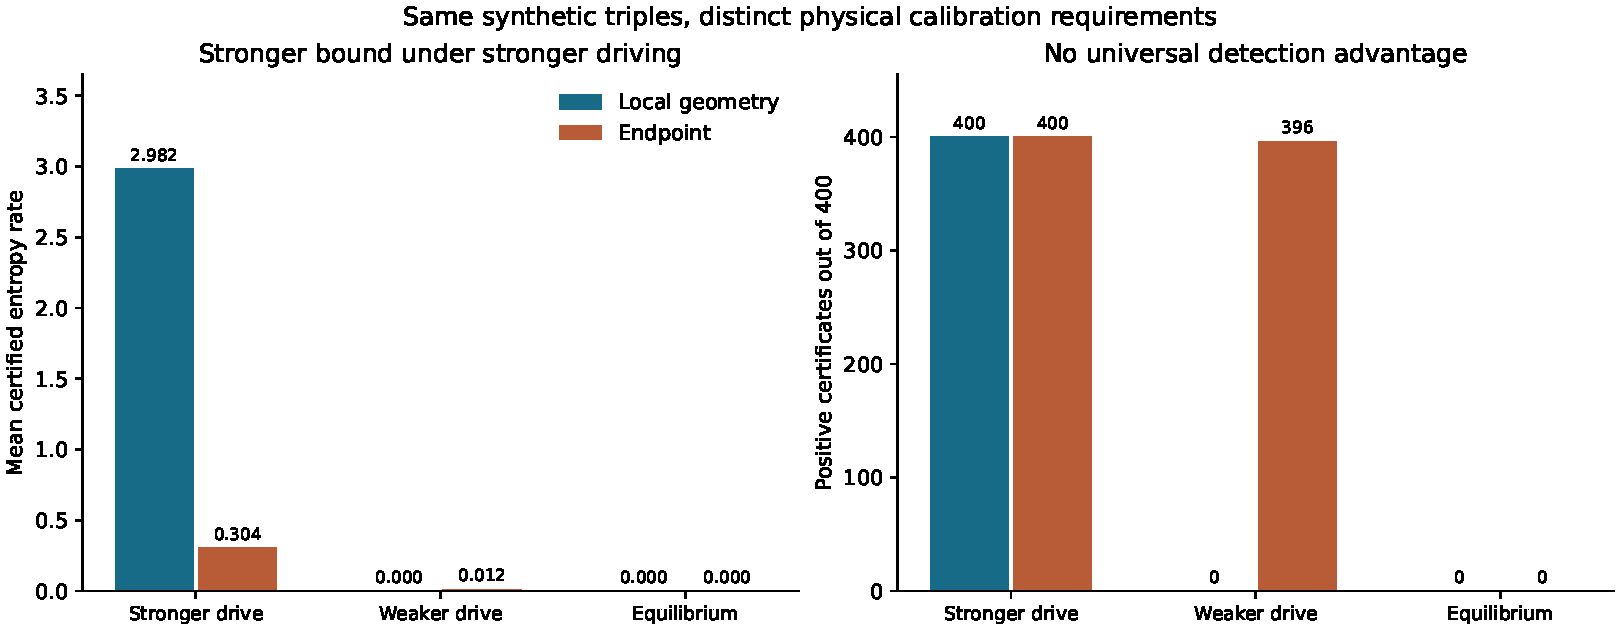
\includegraphics[width=\textwidth]{figures/observed_geometry.pdf}
\caption{The new calibration improves the strong-drive lower bound, while its
finite-time correction prevents a positive certificate for weaker driving.
The two methods use identical synthetic triples.}
\label{fig:og-comparison}
\end{figure}

In the driven case, the geometry certificate has a mean lower bound
$9.811$ times the endpoint mean, certifying on average $33.14\%$ of the actual
rate. The endpoint method certifies $3.38\%$. Neither method overestimates the
known rate in this bank. The Hoeffding geometry certificate is zero in all
1200 datasets: its broad worst-case score range incurs a sampling penalty of
about $24.38$, far larger than the driven score mean. The predeclared
empirical-variance inequality makes the finite-resolution result useful here.

The weakly driven case is an essential limitation. Keeping the same frequency
cap and generator bounds incurs a bias penalty too large for the geometry
certificate, while the endpoint method remains informative in 396 datasets.
A method that resolves the ideal path-law minimum therefore need not dominate
at a finite sampling interval with coarse derivative calibration. We do not
replace the common bounds with values computed from the hidden true frequency.
No equilibrium false positive occurs in this bank. These empirical counts
check implementation behavior; mathematical coverage still rests on the
physical and probabilistic assumptions, not on seeing zero violations.

\section{Resources, reproducibility and application limits}
Each dataset costs 600000 scalar readings, 200000 independent stationary
preparations and $2hn=16000$ units of modeled evolution time for either method.
The complete bank comprises 240 million triples. Preparation and reset time,
clock accuracy, exposure, calibration effort, detector energy and heat are
unmeasured. Equal modeled evolution time is not a claim of equal total
laboratory time or energy.

The release retains all 1200 exact aggregate records, their seeds, the frozen
contract and a full raw triple exemplar for each case. The NPZ archive uses
fixed entry timestamps. Producer checks verify score flooring against rational
arithmetic, pointwise-envelope inflation, uniform rounding penalties, integer
overflow handling, source bindings, aggregate consistency and seed replay.
The independent review rederives the formulas and audits the bank separately.

The practical output is a covered finite-data route to exploit an independently
justified diffusion-geometry envelope. It has not yet been validated for a noisy
laboratory sensor, dependent overlapping records, an uncertain physical clock,
or generator bounds learned from the same data. Those are additional access
and calibration problems, rather than implementation details that can be
assigned zero cost.

\chapter{A covered fallback on the same physical records}
\label{ch:og-combination}

The local-geometry certificate improves the strong-drive benchmark, but its
finite-step penalty removes all positive certificates in the weak-drive case.
The endpoint certificate retains sensitivity there. These complementary
responses suggest a practical composite inference rule. Its justification is
the established union bound; this composition introduces no new statistical
principle and requires no additional acquisition.

\section{Two certificates, one failure budget}
Let $L_G$ and $L_E$ be geometry and endpoint lower bounds computed on the
same fixed independent stationary triples, with component statistical failure
probabilities $\alpha_G$ and $\alpha_E$. Assume the two physical/calibration
contracts hold jointly. Then
\begin{equation}
 \mathbb P\{\max(L_G,L_E)>\sigma\}
 \le \mathbb P\{L_G>\sigma\}+\mathbb P\{L_E>\sigma\}
 \le \alpha_G+\alpha_E.
 \label{eq:og-combined-union}
\end{equation}
The scores may be arbitrarily dependent. The failure allocation and the two
component rules must be fixed for prospective use, or supplied by a separately
justified simultaneous procedure. Here $\alpha_G=\alpha_E=1/40$, so the covered
maximum has statistical failure probability at most $1/20$. A shared pre-test
calibration failure probability is counted once when one joint event validates
both contracts; independent calibration failures can instead be conservatively
summed before adding them. A same-test-data calibration event does not inherit
this guarantee automatically.

The geometry component uses the corrected score of
Chapter~\ref{ch:og-finite}, including the calibrated reading error and score
rounding. The endpoint component uses
\begin{equation}
 Z_s=-(sY_0-Y_{-h})(sY_0-Y_h),\qquad 0\le s\le1,
 \qquad Y_t\in[-1,1].
\end{equation}
Stationarity gives
$\mathbb E Z_s=-s^2 C(0)+2sC(h)-C(2h)$, with
$Z_s\in[-(1+s)^2,1]$. The same empirical-Bernstein construction, with its
uniform score-error correction, supplies a covered lower bound $d$ on the
positive endpoint defect. The seventh-edition physical bridge then yields
\begin{equation}
 L_E=\frac{\Phi(d)}h,\quad 0\le d<1,\qquad
 \Phi(u)=2\sqrt u\operatorname{atanh}\sqrt u,
\end{equation}
with the implementation retaining the existing rational outward enclosure and
its finite-entropy incompatibility handling. The constant follows from the
observable range $R=2$. The implementation requires the common normalized
readout contract; it does not silently use the same constants for a wider
sensor range.

\section{Retrospective reanalysis of the frozen bank}
The equal allocation was introduced after inspecting the primary benchmark.
The following is therefore a retrospective evaluation of a fixed composite
rule, not a new frozen confirmatory experiment. No timing, physical parameter,
record, generator cap or original result was changed. The newly computed
bounds use the exact stored sums and sums of squares from all $1{,}200$
datasets. The original individually valid $\alpha=0.05$ bounds remain in the
primary report; maximizing those original bounds would not by itself retain
a $0.05$ failure guarantee.

\begin{center}
\begin{tabular}{lrrr}
Scenario & Geometry at $0.025$ & Endpoint at $0.025$ & Covered maximum\\
\hline
Strong drive, $\sigma=9$ & $400/400$ & $400/400$ & $400/400$\\
Weak drive, $\sigma=1$ & $0/400$ & $383/400$ & $383/400$\\
Equilibrium, $\sigma=0$ & $0/400$ & $0/400$ & $0/400$\\
\end{tabular}
\end{center}
The geometry component wins every strong-drive dataset; its mean certified
lower bound is $2.887645$, compared with $2.982329$ at its original individual
$0.05$ allocation. The endpoint component supplies every positive weak-drive
result. Its mean bound is $0.00880994$, compared with $0.01196295$ at its
original allocation; detections fall from $396$ to $383$ out of $400$. This is
the observed cost of simultaneous coverage. No reported lower bound exceeds
the known generating entropy in these simulations, which is a numerical
check rather than a proof of coverage beyond the theorem's assumptions.

Every dataset still uses $200{,}000$ independent stationary triples,
$600{,}000$ endpoint readings and $16{,}000$ units of modeled evolution time.
Both scores reuse these same records, so those resources are counted once.
The physical cost of preparation, geometry and clock calibration, exposure,
resetting and energy remains additional. The combined result preserves the
strong-drive benefit while recovering much of the weak-drive endpoint
sensitivity. It does not dominate an individually allocated endpoint test at
every operating point, and it does not justify optimizing the allocation on
the same data without further simultaneous coverage.

\chapter{From ideal access to a physical detector}
\label{ch:dg-entry}

The preceding geometry theorem answers a realization question: what must
every admissible hidden diffusion dissipate to produce a given ideal
observation law? A detector changes the law available to the scientist.
Exposure averages a signal over time, sampling retains selected moments,
and read noise adds uncertainty. Those operations must be included before
an ideal-law theorem becomes an experimental claim.

This extension separates three questions. Does the complete detector law
still identify the ideal law? Can a finite experiment estimate the desired
property with a stated error? How do preparation, read precision, duration
and measurement energy change that error? Different answers to these
questions can hold for the same physical model.

\section{One target, several kinds of access}

Use the stationary cosine-circle family as a reference:
\[
 d\phi_t=\omega\,dt+\sqrt{2\gamma}\,dW_t,
 \qquad Y_t=\cos\phi_t,\qquad \gamma>0.
\]
Its ideal scalar law is reversible. Within the ordinary hidden-diffusion
class of the preceding chapters, its exact compatible minimum is
$\mathcal M=\omega^2/\gamma$. This target is a property of the ideal
law, rather than an attempt to count arbitrary unobserved dissipative
subsystems. The detector considered here retains an exposure average plus
calibrated additive noise.

\begin{center}
\begin{tabular}{p{0.29\textwidth}p{0.60\textwidth}}
\toprule
Available access & Supported conclusion\\
\midrule
Complete densely sampled law; known exposure and independent noise &
The ideal law can be identified under the stated mixing assumptions.
The inverse is an infinite limiting construction.\\[3pt]
Fixed sampling grid after known exposure &
Distinct mixing diffusion mechanisms can have identical complete sampled
laws; an explicit Gaussian example proves this ambiguity.\\[3pt]
Finite stationary trials at fixed positive read noise &
No uniformly finite upper confidence bound exists for the circle minimum
over an unbounded frequency class.\\[3pt]
Known binary hypotheses with fixed read precision &
Passive stationary trials require and suffice at order $\omega^4$;
oriented phase preparation changes this order to $\omega^2$.\\[3pt]
Read precision purchased through the declared law $\nu^2=\kappa/E$ &
Optimized passive and prepared measurement-energy requirements both have
order $\omega^2$. Other apparatus costs remain additional.\\
\bottomrule
\end{tabular}
\end{center}

The count comparison concerns the known pair $\omega$ and $2\omega$
along a specified resonant sequence, at fixed positive diffusion, exposure,
read-noise level and target error. It does not solve estimation over an
arbitrary frequency interval. Preparation means setting the actual phase
to $\pi/2$; selecting a scalar value $Y=0$ does not resolve the two possible
orientations and does not supply the same operation.

\section{Why the resource distinction matters}

Stationary preparation makes the first moment of the exposure vanish.
The leading contrast through a noisy detector then appears in a second
moment. Oriented preparation supplies a first-moment contrast. This familiar
statistical mechanism explains the different trial-count exponents in the
proved example. It is not presented as a new general information law.

The same example shows why a smaller number of trials is insufficient to
establish an energy advantage. Under the explicitly declared sensor model,
passive experiments can spend more energy on read precision and use fewer
trials. The two access classes then share the same measurement-energy
exponent. The result compares orders, not equal optimal constants, and
does not include preparation, resetting, maintaining the drive, exposure
overhead or computation in a total-energy optimum.

The population proofs, finite-access theorems, exact countermodel and
deterministic design table form one account. The new table contains evaluated
analytic bounds, not additional simulated or measured experiments. The
earlier frozen simulation bank remains a separate numerical validation of
the finite-resolution certificate. Independent internal review checks both
layers; external peer review and prospective detector calibration remain
open.

The next practical dependency is a detector-specific joint calibration
guarantee for local volatility and the short-time statistics used in the
entropy certificate. Existing motion-blur correction and noisy-diffusion
inference provide essential baselines. Their assumptions must be carried
through the physical entropy bound, including selection and dependence
between calibration and test records.

\chapter{What calibrated exposure preserves at the population level}
\label{ch:dg-recovery}

Finite exposure changes a diffusion observation before measurement noise is
added. In particular, a boxcar average of a continuous signal is continuously
differentiable and has zero quadratic variation. The local geometry theorem
therefore cannot be applied directly to an exposed trace as if it were the
original diffusion coordinate. The question here is different: does the
complete exposed observation law still determine the ideal law from which
that trace came?

Under the assumptions below, the answer is yes, even after a known independent
additive noise channel. The recovery uses dense temporal population access
and an infinite limiting reconstruction. It does not provide a stable
finite-data inverse or recover local quadratic variation by differentiating
noisy samples. The constituent deconvolution and averaging arguments are
established mathematical tools; historical priority is not asserted.

\section{Detector and access model}

Let $Y=(Y_t)_{t\in\mathbb R}$ be a real stationary continuous process,
bounded by a finite deterministic constant, and write $\mu=\mathbb E Y_0$.
Assume
\begin{equation}
 \operatorname{Cov}(Y_0,Y_t)\longrightarrow0
 \quad\hbox{as }|t|\longrightarrow\infty.
 \label{eq:dg-covariance-mixing}
\end{equation}
This condition is satisfied by a smooth bounded coordinate of a stationary
compact connected uniformly elliptic diffusion. A known exposure width
$\tau>0$ produces the causal boxcar signal
\begin{equation}
 Z_t=(A_\tau Y)_t
      :=\frac1\tau\int_{t-\tau}^tY_s\,ds.
 \label{eq:dg-exposure}
\end{equation}
Let $\mathcal T$ be a known countable dense subset of the real time axis.
At each distinct $t\in\mathcal T$, the retained measurement is
\begin{equation}
 B_t=Z_t+\xi_t,
 \label{eq:dg-readout}
\end{equation}
where the $\xi_t$ are independent of $Y$, independent across distinct
timestamps, and have a known probability law $\nu$. The known noise law
need not have finite variance or a nowhere-zero characteristic function for
the population uniqueness statement. Its independence and calibration are
part of the detector contract.

The accessible research object in this section is the complete joint law of
$(B_t)_{t\in\mathcal T}$, rather than one finite record. Repeated samples
of a finite collection of timestamps do not automatically supply this
infinite family of joint distributions. The clock, exposure rule, and noise
law are common to every model being compared.

\section{Noise removal as an identifiability statement}

\begin{lemma}[Known additive convolution on a bounded latent law]
\label{lem:dg-bounded-convolution}
Let $P$ and $Q$ be compactly supported probability laws on $\mathbb R^k$,
and let $N$ be any probability law on $\mathbb R^k$. If
$P*N=Q*N$, then $P=Q$.
\end{lemma}

\begin{proof}
The characteristic function $\widehat N$ is continuous and equals one at
the origin, so it is nonzero on some neighborhood of zero. The convolution
identity implies $\widehat P=\widehat Q$ on that neighborhood. Compact
support makes both characteristic functions real analytic on
$\mathbb R^k$ (indeed entire after complexification). Analytic uniqueness
therefore extends the equality to all real arguments. Uniqueness of
characteristic functions gives $P=Q$.
\end{proof}

Apply this lemma at any finite set of distinct timestamps, with the known
noise law $N=\nu^{\otimes k}$. Equality of the noisy record laws implies
equality of the corresponding finite-dimensional laws of $Z$. Since $Z$ is
continuous, its values on the countable dense set determine its law on
$C(\mathbb R)$, equipped with uniform convergence on compact intervals.
Thus the complete noisy law identifies the complete exposure law.

This proof does not divide by the noise characteristic function at its
zeros. It uses bounded latent support and uniqueness of analytic
continuation; it supplies no stability estimate for that continuation. If
bounded support is dropped, a standard sufficient replacement is a noise
characteristic function that is nowhere zero. These are different
identifiability contracts. Known correlated additive noise can also be
treated if its complete joint laws are supplied and remain independent of
the signal; knowing only its one-time marginal would not suffice.

\subsection{What infinitely dense independent readouts can recover}

For the iid noise contract, dense access permits a stronger statement that
does not require bounded signal amplitude. Let $Z$ have continuous finite
real-valued paths and let $B_t=Z_t+\xi_t$ be observed on the countable dense
set, with the same known iid noise independent of $Z$. Then the complete
continuous exposure path is a measurable function of the infinitely dense
noisy record, almost surely.

To prove this, fix a target $t$ in the dense set and a deterministic sequence
of distinct available timestamps $t_j\to t$. For any fixed real $u$, the
bounded complex observations satisfy
\begin{equation}
 \frac1n\sum_{j=1}^n e^{iuB_{t_j}}
 \longrightarrow e^{iuZ_t}\widehat\nu(u)
 \quad\hbox{almost surely}.
 \label{eq:dg-dense-noise-average}
\end{equation}
Conditioned on the entire continuous $Z$ path, the centered summands are
independent bounded variables. The independent-variable strong law applies
because the sum of their variances divided by $j^2$ is finite. Their average
conditional means converge to the right-hand side by continuity of $Z$.
The argument uses no moment of $\xi_t$.

Choose a countable sequence $u_k\to0$ with $u_k\ne0$. The known noise
characteristic function is nonzero for all sufficiently large $k$.
Dividing the limits in~\eqref{eq:dg-dense-noise-average} by
$\widehat\nu(u_k)$ determines $e^{iu_kZ_t}$, and
\[
 Z_t=\lim_{k\to\infty}
       \frac{\operatorname{Im}(e^{iu_kZ_t})}{u_k}
\]
removes the phase ambiguity. A countable intersection of probability-one
events recovers every dense-set $Z_t$; continuity supplies the full path.
All operations are limits of measurable coordinate functions, with an
arbitrary default on the null set where the limits fail.

Consequently the main injectivity theorem below also holds with boundedness
replaced by finite second moment, using this dense iid reconstruction and
the same covariance-decay assumption. The compact diffusion application
remains bounded. The proposition spends infinitely many independent
readouts in arbitrarily small time neighborhoods. It is not a claim that
faster sampling makes actual sensor errors independent: overlapping
exposures, photon reuse, memory, or correlated readout noise can invalidate
the stipulated iid contract. The earlier bounded-law convolution argument
is still useful for known correlated noise at the population-law level,
where pathwise separation from one continuous record need not hold.

\section{An explicit finite-window reconstruction and its limit}

Continuity of $Y$ gives the pathwise identity
\begin{equation}
 \tau Z'_t=Y_t-Y_{t-\tau}.
 \label{eq:dg-derivative}
\end{equation}
The derivative is a measurable functional of the ideal $C^1$ exposure path,
for example the limit of rational difference quotients. For $N\geq1$ set
\begin{equation}
 \mathcal R_N Z(t)
 :=\mathbb E Z_0+
 \tau\sum_{k=0}^{N-1}\left(1-\frac{k}{N}\right)Z'_{t-k\tau}.
 \label{eq:dg-triangular-reconstruction}
\end{equation}
Telescoping gives the exact relation
\begin{equation}
 \mathcal R_N Z(t)
 =Y_t-\left\{\frac1N\sum_{j=1}^NY_{t-j\tau}-\mu\right\}.
 \label{eq:dg-reconstruction-error}
\end{equation}
Only a window whose length grows as $N\tau$ is used at each finite $N$,
but exact derivatives of the exposed path are required.

\begin{theorem}[Dense-law injectivity through boxcar exposure and known noise]
\label{thm:dg-injectivity}
Within the bounded continuous stationary class satisfying
Equation~\eqref{eq:dg-covariance-mixing}, equality of the noisy dense-time
laws in~\eqref{eq:dg-readout}, for a common known boxcar width and noise
law, implies equality of the ideal continuous path laws of $Y$.
\end{theorem}

\begin{proof}
The preceding lemma identifies the common continuous law of $Z$.
Stationarity gives $\mathbb E Z_0=\mu$. By
Equation~\eqref{eq:dg-reconstruction-error},
\begin{align}
 \mathbb E|\mathcal R_N Z(t)-Y_t|^2
 &=\frac1{N^2}\sum_{i,j=1}^N
          \operatorname{Cov}(Y_0,Y_{(i-j)\tau})\notag\\
 &=\frac{\operatorname{Var}(Y_0)}N
   +\frac2{N^2}\sum_{j=1}^{N-1}(N-j)
                \operatorname{Cov}(Y_0,Y_{j\tau})
 \longrightarrow0.
 \label{eq:dg-mean-square-recovery}
\end{align}
For the last limit, bound the finite initial part of the covariance sum by
a constant times $N^{-1}$, and use arbitrarily small covariance on its
remaining tail. The same conclusion holds jointly at every finite set of
times, by summing their mean-square errors. The law of each
$\mathcal R_N Z$ is fixed by the common exposure law, so the limiting
finite-dimensional laws of $Y$ agree. Continuity again identifies the full
path laws.
\end{proof}

An explicitly calibrated covariance-decay bound gives a finite-window
population estimate. If
$|\operatorname{Cov}(Y_0,Y_t)|\leq C e^{-\kappa|t|}$ for $C<\infty$
and $\kappa>0$, then
\begin{equation}
 \mathbb E|\mathcal R_N Z(t)-Y_t|^2
 \leq\frac{C}{N}\coth(\kappa\tau/2).
 \label{eq:dg-reconstruction-rate}
\end{equation}
This controls truncation of an ideal derivative reconstruction. It does
not control estimation of $Z'$ from finitely many noisy or exposed readings.
For example, if a derivative approximation has root mean-square error at
most $\delta$ at each of the retained times, and the stationary mean has
error at most $\delta_\mu$, the triangle inequality gives only
\[
 \|\widehat{\mathcal R_N Z}(t)-Y_t\|_2
 \leq \sqrt{\frac C N\coth(\kappa\tau/2)}
       +\frac{\tau(N+1)}2\,\delta+\delta_\mu.
\]
Increasing the reconstruction window can amplify derivative error. Any
finite-data use must pay for both terms under an explicit detector model.

\section{The spectral obstruction and a derivative-free population inverse}

The exposure multiplier at frequency $\lambda$ is
\begin{equation}
 H_\tau(\lambda)
 =e^{-i\lambda\tau/2}\frac{\sin(\lambda\tau/2)}{\lambda\tau/2},
 \qquad H_\tau(0)=1.
 \label{eq:dg-transfer}
\end{equation}
It vanishes exactly at $\lambda=2\pi k/\tau$, $k\in\mathbb Z\setminus\{0\}$.
The decay assumption excludes spectral atoms at those frequencies. The
minimal spectral premise for recovering a particular $Y$ is that its
spectral measure assign zero mass to those zeros; full mixing is a convenient
sufficient assumption.

For completeness, the usual Landweber reconstruction gives a second proof
that does not explicitly differentiate $Z$. On the stationary $L^2$ shift
space let $A=A_\tau$ and $T=A^*A$, so $0\preceq T\preceq I$. Define
\begin{equation}
 \mathcal L_N Z
   =\sum_{j=0}^{N-1}(I-T)^jA^*Z.
 \label{eq:dg-landweber}
\end{equation}
Since $Z=AY$,
\[
 \mathcal L_N Z=[I-(I-T)^N]Y.
\]
The spectral theorem gives $L^2$ convergence to $Y$ exactly when $Y$ has no
component in $\ker A$. The kernel consists of the nonzero boxcar-resonant
spectral modes above; the stationary mean is preserved because $H_\tau(0)=1$.
Each iterate is a finite linear combination of finite-window averages of
$Z$ and is therefore a fixed measurable function of its continuous path.

This inverse is also not uniformly stable as $N\to\infty$. Its operator
norm is at most $\sqrt N$, because for $0\leq x\leq1$,
\[
 \sqrt{x}\sum_{j=0}^{N-1}(1-x)^j
 =\frac{1-(1-x)^N}{\sqrt x}
 \leq\min\{N\sqrt x,x^{-1/2}\}\leq\sqrt N.
\]
At $x=0$ the expression is defined by its zero limit for fixed $N$.
For a stationary $L^2$ perturbation of the entire input process, this bounds
its amplification by $\sqrt N$. It is not an assertion that a finite
collection of independent point-noise values forms a directly integrable
continuous error process.

The spectral bias is explicitly
\[
 \|\mathcal L_N AY-Y\|_2^2
 =\int(1-|H_\tau(\lambda)|^2)^{2N}\,d\mu_Y(\lambda).
\]
Vanishing mass at exact zeros ensures convergence; a useful finite-error
rate additionally needs quantitative control of spectral mass near the
zeros and at large frequencies. Injectivity alone supplies no such rate.

\section{Consequences for the compatible diffusion minimum}

Every admissible compact connected uniformly elliptic hidden diffusion in
the observed-geometry chapter has a bounded smooth detector and exponentially
decaying centered correlations. Consequently, if its ideal coordinate is
observed through the detector contract here, the complete noisy dense-time
law determines its ideal continuous observation law.

In particular, fix the noisy exposed law generated by the stationary
cosine-circle process with parameters $\gamma>0$ and $\omega$, with the
same calibrated detector channel used in all compatible models. Every
compatible admissible hidden diffusion then has the same ideal law as that
circle. The earlier attained minimum therefore remains
\begin{equation}
 \min\sigma=\omega^2/\gamma.
 \label{eq:dg-minimum-preserved}
\end{equation}
The circle with the stated detector is feasible, so this is an attained
minimum, not only a lower bound. The result concerns entropy production in
the target hidden diffusion, not the unmodeled energy consumed by the
detector or the readout process.

The identification uses infinitely rich population information. It does
not show that a finite noisy experiment can attain the same accuracy as a
noiseless high-bandwidth experiment. In particular, $Z$ itself has zero
quadratic variation. Local geometry is recovered only after an appropriate
limiting reconstruction of the ideal law, rather than by applying the
previous local formula directly to $Z$ or $B$.

\section{When the width itself is identifiable}

Here and in the preceding compatible-minimum statement, the diffusion
assumptions are those of the earlier observed-geometry class: a smooth compact
connected manifold without boundary, smooth coefficients and strictly positive
stationary density, uniform ellipticity, and ordinary reversal of the complete
hidden state. No unspecified boundary condition or generalized reversal is
included by the shorter phrase ``compact elliptic'' below.

Within the compact elliptic model class, a known boxcar shape has a further
population property: its width can be identified from the exposed law even
if that width was not initially supplied. Assume the detector is nonconstant.
Let $f$ now denote the centered detector, and use the complex
$L^2(\pi)$ inner product. The symmetric part of the generator has a
Poincar\'e gap, so its mean-zero semigroup decays exponentially and the
resolvent exists at every $i\lambda$, $\lambda\in\mathbb R$.
For $u=(i\lambda-L)^{-1}f$, the ideal power spectral density is
\begin{equation}
 S_Y(\lambda)
 =2\operatorname{Re}\langle f,(i\lambda-L)^{-1}f\rangle_\pi
 =2\int_M\nabla\overline u^{\mathsf T}D\nabla u\,d\pi
 >0.
 \label{eq:dg-positive-spectrum}
\end{equation}
The identity follows from $f=(i\lambda-L)u$ and skew-adjointness of the
stationary current term. The Dirichlet form vanishes only for constant $u$;
in the mean-zero subspace this would force $u=0$ and then $f=0$, contrary
to the nonconstant detector assumption.

The centered exposed spectrum is
$S_Z(\lambda)=|H_\tau(\lambda)|^2S_Y(\lambda)$. Its zero set is
therefore exactly the nonzero boxcar frequencies. The smallest positive
zero equals $2\pi/\tau$ and identifies $\tau$. Known-noise deconvolution
may first be used to identify the exposure law; no finite-variance noise
assumption is needed if the bounded-law uniqueness argument is used.
This proposition assumes the boxcar shape, nonconstant diffusion detector,
continuous population spectrum and calibrated time. A constant signal has
no such width information. Estimating an exact spectral zero from a finite
noisy record is a separate problem, and an unknown general response kernel
is not identified by this argument.

\section{Necessary distinctions}

The mathematical ingredients have substantial prior art. Landweber's 1951
iteration is an established inverse method. Known-error deconvolution with
characteristic-function zeros is treated, under quantitative assumptions,
by Hall and Meister (2007). Nakakita and Uchida (2020) already estimate an
unknown exposure-to-frame ratio for convolutionally observed diffusions in
a shrinking-exposure, increasing-duration regime. The fixed-width
full-law argument here is a different observation regime, not the first
inference of an unknown shutter parameter. Markov-generator resolvent
formulas for power spectra are also established; Gupta and Khammash (2022)
provide a close explicit use for stochastic reaction networks. The focused
primary-source audit is recorded separately in this research phase. These
comparisons leave historical priority for any narrower combination open.

A stationary periodic signal with uniform random phase at frequency
$2\pi/\tau$ is erased exactly by the boxcar. Such a process is stationary
and can be ergodic under the full continuous time-shift group while failing
mixing and ergodicity under the sampled $\tau$-shift. Continuous-flow
ergodicity alone is therefore not a sufficient replacement for the
assumptions used here.

A fixed discrete sampling grid also supplies less information than the
dense-time law in the theorem. Continuity does not reconstruct an exposed
path between grid points. Exact aliasing or different hidden dynamics can
survive fixed-grid exposure data, and no claim of injectivity for that
access model follows from this chapter.

Finally, the inverse has no uniform stability bound over all admissible
mixing signals. Boxcar multipliers become arbitrarily small near their
zeros and at high frequency. Additional bandwidth, dynamical, detector or
resource restrictions are needed for a useful finite-error conclusion.
Population identifiability, physical attainability, finite-data confidence,
and experimental energy are separate claims throughout this argument.

\chapter{Finite detector access to a sharp physical minimum}
\label{ch:dg-finite-access}

An ideal observation law can determine a physical minimum while a finite
apparatus record remains unable to bound that minimum from above. The
distinction can be quantified in the same circle family. At fixed exposure
and positive read-noise variance, passive stationary trials and trials with
an oriented phase preparation have different sample requirements for a
specified binary comparison. Allowing read precision to consume a declared
measurement energy changes that comparison again. This chapter proves all
three statements in one explicit detector model.

The target is the already attained minimum compatible with the ideal
cosine-circle law,
\begin{equation}
 \mathcal M(\omega)=\frac{\omega^2}{\gamma},\qquad \gamma>0.
 \label{eq:dg-minimum-target}
\end{equation}
It is not an upper bound on the actual entropy of every hidden realization:
an invisible independently dissipating subsystem would already rule out
that stronger interpretation under perfect access. Here the detector
obstructs inference of a functional that is sharply fixed by the ideal
observed law itself.

\section{One fixed exposure and its moments}

Let the target diffusion satisfy
\[
 d\phi_t=\omega\,dt+\sqrt{2\gamma}\,dW_t\pmod{2\pi}.
\]
An exposure of fixed length $\tau>0$ yields
\begin{equation}
 A_\omega=\frac1\tau\int_0^\tau\cos\phi_t\,dt,
 \qquad X_\omega=A_\omega+\xi,
 \qquad \xi\sim N(0,\nu^2),\quad\nu>0,
 \label{eq:dg-exposure-record}
\end{equation}
where the read noise is independent of the entire target trajectory.
The parameters $\gamma$, $\tau$, and $\nu$ are known and fixed unless a
different precision law is explicitly declared below. In every case
$|A_\omega|\leq1$.

For passive stationary trials, the initial phase is uniform and
$\mathbb E A_\omega=0$. Define $V(\omega)=\mathbb E A_\omega^2$.
The covariance
$\mathbb E[\cos\phi_0\cos\phi_t]
 =\tfrac12e^{-\gamma|t|}\cos(\omega t)$ gives
\begin{equation}
 V(\omega)=\frac1{\tau^2}\operatorname{Re}
 \left\{\frac\tau z-\frac{1-e^{-z\tau}}{z^2}\right\},
 \qquad z=\gamma-i\omega.
 \label{eq:dg-exposure-variance}
\end{equation}
This follows by integrating the covariance over the exposure square, or
equivalently by integrating
$\tau^{-2}(\tau-t)e^{-\gamma t}\cos(\omega t)$ over $0\leq t\leq\tau$.

For an explicit asymptotic comparison, use the resonant sequence
\begin{equation}
 \omega_m=2\pi m/\tau,\quad m=1,2,\ldots,
 \qquad a_0=1-e^{-\gamma\tau}>0.
 \label{eq:dg-resonant-family}
\end{equation}
At these frequencies,
\begin{equation}
 V(\omega)=
 \frac{(\gamma\tau+a_0)\omega^2
       +(\gamma\tau-a_0)\gamma^2}
      {\tau^2(\gamma^2+\omega^2)^2}
 \sim\frac{\gamma\tau+a_0}{\tau^2\omega^2}.
 \label{eq:dg-resonant-variance}
\end{equation}
In particular,
\begin{equation}
 \Delta_V(\omega):=|V(\omega)-V(2\omega)|
 \sim\frac{3(\gamma\tau+a_0)}{4\tau^2\omega^2}.
 \label{eq:dg-variance-gap}
\end{equation}
All asymptotic statements in this chapter fix the detector and confidence
constants and take $m\to\infty$ along this sequence.

Two moment bounds hold uniformly over the initial phase distribution,
and hence apply to both stationary and prepared trials. Set
\begin{align}
 H_2&=\frac{[2+\gamma\tau+\sqrt{2\gamma\tau}]^2}{\tau^2},\\
 H_4&=\frac{8[(2+\gamma\tau)^4+12\gamma^2\tau^2]}{\tau^4}.
 \label{eq:dg-ito-constants}
\end{align}
For $\omega\ne0$,
\begin{equation}
 \mathbb E A_\omega^2\leq\frac{H_2}{\omega^2},
 \qquad
 \mathbb E A_\omega^4\leq\frac{H_4}{\omega^4}.
 \label{eq:dg-ito-moments}
\end{equation}
To see this, It\^o's formula gives
\begin{equation}
 \omega\tau A_\omega
 =\sin\phi_\tau-\sin\phi_0
   +\gamma\int_0^\tau\sin\phi_s\,ds
   -\sqrt{2\gamma}\int_0^\tau\cos\phi_s\,dW_s.
 \label{eq:dg-ito-exposure}
\end{equation}
The bounded part has absolute value at most $2+\gamma\tau$. For
$M_t=\int_0^t\cos\phi_s\,dW_s$, It\^o isometry gives
$\mathbb E M_\tau^2\leq\tau$ and the fourth-moment identity gives
\[
 \mathbb E M_\tau^4
 =6\mathbb E\int_0^\tau M_s^2\cos^2\phi_s\,ds
 \leq6\int_0^\tau s\,ds=3\tau^2.
\]
Minkowski's inequality proves the second-moment bound. The elementary
inequality $(x+y)^4\leq8(x^4+y^4)$ proves the fourth-moment bound.
No independence between the bounded and martingale terms is assumed.

\section{A finite record cannot provide a uniformly finite upper bound}

Fix $n$ predetermined exposure windows, each of width $\tau$, from a
stationary trajectory. The windows may overlap and their latent exposure
values may be correlated. Let $P_\omega^{(n)}$ be the law of their noisy
records under independent Gaussian read errors, and let
$Q^{(n)}=N(0,\nu^2I_n)$. Convexity of relative entropy under Gaussian
mixing yields
\begin{equation}
 D(P_\omega^{(n)}\Vert Q^{(n)})
 \leq\frac{\mathbb E\|A_\omega^{(n)}\|^2}{2\nu^2}
 =\frac{nV(\omega)}{2\nu^2}
 \leq\frac{nH_2}{2\nu^2\omega^2}.
 \label{eq:dg-mixture-kl}
\end{equation}
Indeed, conditional on the exposure vector, the readout is Gaussian with
that vector as its mean and covariance $\nu^2I_n$. Its relative entropy
to $Q^{(n)}$ is the squared mean divided by $2\nu^2$; mixing can only
decrease the relative entropy. Pinsker's inequality therefore implies
$\operatorname{TV}(P_\omega^{(n)},Q^{(n)})\to0$ as
$\omega\to\infty$, whereas $\mathcal M(\omega)\to\infty$.

\begin{theorem}[Upper-confidence obstruction for the sharp minimum]
\label{thm:dg-upper-obstruction}
Suppose a measurable extended-valued statistic $U$ of this finite record
satisfies
\[
 P_\omega^{(n)}\{U\geq\mathcal M(\omega)\}\geq1-\alpha
 \quad\hbox{for every }\omega>0,
 \qquad 0<\alpha<1.
\]
Then $Q^{(n)}\{U=+\infty\}\geq1-\alpha$. In particular, no such
uniformly covered upper bound is finite almost surely under even one of the
finite-$\omega$ record laws. The conclusion concerns the fixed finite
detector design and unbounded frequency class just stated.
\end{theorem}

\begin{proof}
For every finite $K$, sufficiently large $\omega$ has
$\mathcal M(\omega)>K$, so
\[
 Q^{(n)}\{U>K\}
 \geq1-\alpha-\operatorname{TV}(P_\omega^{(n)},Q^{(n)}).
\]
Let $\omega\to\infty$ and then $K\to\infty$ to obtain the first
assertion. Each Gaussian mixture $P_\omega^{(n)}$ has a strictly positive
density everywhere on $\mathbb R^n$, and is therefore mutually absolutely
continuous with $Q^{(n)}$. If $U$ were finite almost surely under any one
$P_\omega^{(n)}$, it would also be finite almost surely under $Q^{(n)}$,
contradicting the first assertion.
\end{proof}

The pure-noise law is a limiting reference, not necessarily a finite-parameter
member of the model class. Accordingly, the theorem does not claim
$P_\omega^{(n)}\{U=+\infty\}\geq1-\alpha$ at every fixed $\omega$.
The general quantitative statement is
\[
 P_\omega^{(n)}\{U=+\infty\}
 \geq1-\alpha-\operatorname{TV}(P_\omega^{(n)},Q^{(n)}).
\]
A calibrated frequency or generator envelope removes the unbounded class
used in this argument. Adaptive timing, adaptive precision, or a growing
number of measurements needs its own sequential analysis; it is not included
in this fixed-design theorem.

\section{Matching passive sample requirements at fixed precision}

Now compare the known alternatives $\omega$ and $2\omega$ using
independent stationary trials, each with a fresh stationary preparation and
one exposure. Define $n^*_{\rm passive}(\omega,\epsilon)$ as the minimum
number of such trials needed for equal-prior binary error at most
$\epsilon\in(0,1/2)$. An upper construction below bounds each of the two
conditional errors by $\epsilon$, which is a stronger guarantee.

The zero stationary mean improves the mixture bound for independent trials.
Let $P$ be the one-record law of $A+\xi$, $Q=N(0,\nu^2)$, and let
$A'$ be an independent copy of $A$. Direct multiplication of Gaussian
likelihood ratios gives
\begin{equation}
 \chi^2(P\Vert Q)
 =\mathbb E e^{AA'/\nu^2}-1
 =\sum_{k=1}^\infty
       \frac{(\mathbb E A^k)^2}{k!\nu^{2k}}.
 \label{eq:dg-mixture-chi-square}
\end{equation}
Bounded $A$ justifies termwise expectation. Since $\mathbb E A=0$ and
$|\mathbb E A^k|\leq\mathbb E A^2=V$ for every $k\geq2$,
\begin{equation}
\chi^2(P\Vert Q)\leq C_{\nu,0} V^2,
 \qquad C_{\nu,0}=e^{1/\nu^2}-1-1/\nu^2>0.
 \label{eq:dg-stationary-chi-square}
\end{equation}
For the stationary circle the bound is stronger. Shifting every phase by
$\pi$ preserves its stationary path law and changes $A$ to $-A$.
All odd moments therefore vanish, and retaining only the even terms in
Equation~\eqref{eq:dg-mixture-chi-square} gives
\begin{equation}
 \chi^2(P\Vert Q)\leq C_\nu V^2,
 \qquad C_\nu=\cosh(1/\nu^2)-1.
 \label{eq:dg-symmetric-chi-square}
\end{equation}
The sharper circle constant is used in the count bounds below.
For independent trials, relative entropy tensorizes. Using
$D\leq\log(1+\chi^2)\leq\chi^2$ and the triangle inequality for total
variation,
\[
 \operatorname{TV}(P_\omega^{\otimes n},P_{2\omega}^{\otimes n})
 \leq\sqrt{\frac{nC_\nu}{2}}\{V(\omega)+V(2\omega)\}.
\]
The optimal equal-prior error is $(1-\operatorname{TV})/2$. Hence a necessary
sample count is
\begin{equation}
 n\geq
 \frac{2(1-2\epsilon)^2}
      {C_\nu\{V(\omega)+V(2\omega)\}^2}.
 \label{eq:dg-passive-necessary}
\end{equation}
The constant can be numerically weak, especially for small $\nu$; a bound
below one is vacuous as an integer-count constraint. The asymptotic order
remains informative at fixed positive $\nu$.

For a matching upper bound, use the sample mean of $X^2$ and put its threshold
midway between $\nu^2+V(\omega)$ and $\nu^2+V(2\omega)$. Gaussian moments
and $|A|\leq1$ give
\begin{align}
 \operatorname{Var}(X^2)
 &=\mathbb E A^4-V^2+4\nu^2V+2\nu^4\notag\\
 &\leq S_\nu(V):=(1+4\nu^2)V-V^2+2\nu^4.
 \label{eq:dg-square-variance}
\end{align}
Chebyshev's inequality then bounds each conditional error by $\epsilon$
whenever
\begin{equation}
 n\geq
 \left\lceil
 \frac{4\max\{S_\nu(V(\omega)),S_\nu(V(2\omega))\}}
      {\epsilon\,\Delta_V(\omega)^2}
 \right\rceil.
 \label{eq:dg-passive-sufficient}
\end{equation}
A simpler valid numerator is $4(1+6\nu^2+3\nu^4)$, obtained by bounding
$\mathbb E X^4$ directly. The more precise expression above improves
constants without changing the access or confidence criterion.

Equations~\eqref{eq:dg-resonant-variance}--\eqref{eq:dg-variance-gap}
and the two sample bounds prove
\begin{equation}
 n^*_{\rm passive}(\omega_m,\epsilon)=\Theta(\omega_m^4)
      =\Theta(\mathcal M(\omega_m)^2).
 \label{eq:dg-passive-rate}
\end{equation}
The constants may depend on fixed $\gamma$, $\tau$, $\nu$, and
$\epsilon$. This is a binary comparison along the declared sequence,
not a minimax theorem for estimating an arbitrary unknown frequency from
an arbitrary trajectory. Nonoverlapping windows from one stationary
trajectory are not automatically independent stationary preparations.

\section{Matching requirements with an oriented phase preparation}

Suppose each independent trial can instead start from the actual known
phase $\phi_0=\pi/2$, under both hypotheses. Its expectation during the
exposure is $\mathbb E\cos\phi_t=-e^{-\gamma t}\sin(\omega t)$.
At resonance, the one-record mean is
\begin{equation}
 \mu(\omega)=-\frac{a_0\omega}{\tau(\gamma^2+\omega^2)},\qquad
 \Delta_\mu(\omega)
 =\frac{a_0|\omega|\,|2\omega^2-\gamma^2|}
        {\tau(\gamma^2+\omega^2)(\gamma^2+4\omega^2)}
 \sim\frac{a_0}{2\tau|\omega|}.
 \label{eq:dg-prepared-mean}
\end{equation}
The gap is positive for sufficiently large resonant frequencies; at
$\omega^2=\gamma^2/2$ this particular mean test has zero gap and supplies
no discrimination guarantee.

Since $A\in[-1,1]$, its centered version is sub-Gaussian with variance proxy
one. Adding the independent Gaussian read noise gives proxy $1+\nu^2$.
The sample-mean midpoint test therefore bounds each conditional error by
$\epsilon$ with the sufficient count
\begin{equation}
 n\geq
 \left\lceil
 \frac{8(1+\nu^2)\log(1/\epsilon)}{\Delta_\mu(\omega)^2}
 \right\rceil.
 \label{eq:dg-prepared-sufficient}
\end{equation}

A lower bound of the same order follows without assuming stationarity.
The uniform second-moment bound~\eqref{eq:dg-ito-moments} and the
Gaussian-mixture relative-entropy inequality give, for any common fixed
phase-preparation rule,
\[
 D(P_\omega^{\otimes n}\Vert Q^{\otimes n})
 \leq\frac{nH_2}{2\nu^2\omega^2}.
\]
For the pair $\omega,2\omega$, Pinsker and the triangle inequality imply
\[
 \operatorname{TV}(P_\omega^{\otimes n},P_{2\omega}^{\otimes n})
 \leq\frac{3\sqrt{nH_2}}{4\nu|\omega|}.
\]
An equal-prior error at most $\epsilon$ consequently requires
\begin{equation}
 n\geq\frac{16\nu^2(1-2\epsilon)^2\omega^2}{9H_2}.
 \label{eq:dg-prepared-necessary}
\end{equation}
The construction and obstruction together prove
\begin{equation}
 n^*_{\rm prepared}(\omega_m,\epsilon)=\Theta(\omega_m^2)
         =\Theta(\mathcal M(\omega_m)).
 \label{eq:dg-prepared-rate}
\end{equation}

The preparation need not be a perfect point mass. A known initial phase
law with $\mathbb E\cos\phi_0=0$ and a fixed nonzero
$r=\mathbb E\sin\phi_0$ multiplies the mean in
Equation~\eqref{eq:dg-prepared-mean} by $r$, preserving the exponent with
a sufficient-count constant proportional to $r^{-2}$. Merely preparing
$Y_0=\cos\phi_0=0$ does not establish this condition: an equal mixture of
$\pi/2$ and $3\pi/2$ has $r=0$ and cancels the mean signal.

These prepared records are not stationary entropy-production records and are
not inserted into the stationary local-defect certificate. They distinguish
two generators whose stationary ideal laws have the target minima
$\mathcal M(\omega)$ and $4\mathcal M(\omega)$. A phase preparation is a
change in permitted access, with its own apparatus and energy requirements.

\section{What changes when read precision consumes energy}

The previous exponents count trials at fixed positive read-noise variance.
They are not total-energy exponents. To make that distinction explicit,
consider the following additional, declared sensor model:
\begin{equation}
 \nu_i^2=\frac{\kappa}{E_i},\qquad \kappa>0,
 \quad E_i>0,
 \label{eq:dg-sensor-energy-law}
\end{equation}
where $E_i$ is the measurement energy allocated to record $i$. This is an
assumed calibration law, not a universal thermodynamic law. The finite
energy schedule is fixed before the data, and read errors remain independent
of the target and each other. Preparation, reset, exposure duration, and
actuation costs are not included in $E_i$.

Let $E_{\rm meas}=\sum_iE_i$, and use the Gaussian reference with diagonal
variances $\kappa/E_i$. Conditional Gaussian relative entropy and
Equation~\eqref{eq:dg-ito-moments} imply
\begin{equation}
 D(P_\omega\Vert Q)
 \leq\sum_i\frac{E_i\mathbb E A_{\omega,i}^2}{2\kappa}
 \leq\frac{H_2E_{\rm meas}}{2\kappa\omega^2}.
 \label{eq:dg-energy-kl}
\end{equation}
This bound permits correlated latent exposures at predetermined windows,
provided each has the stated dynamics and duration. The initial phases can
follow the same fixed preparation rule under both hypotheses. The
corresponding pairwise Pinsker bound gives the necessary measurement energy
\begin{equation}
 \boxed{\displaystyle
 E_{\rm meas}\geq
 \frac{16\kappa(1-2\epsilon)^2\omega^2}{9H_2}.}
 \label{eq:dg-energy-necessary}
\end{equation}
The proof does not cover an energy schedule adaptively selected from noisy
records or an intervention that changes the dynamics during exposure.

Passive stationary trials can attain the same exponent by buying more
precision per record. Fix $c>0$ and use
$E_i=c\omega^2$ under both alternatives, so
$\nu_i^2=\kappa/(c\omega^2)$. This design is permitted because the
binary candidate pair is known. Let
\begin{equation}
 B_c=H_4+\frac{6\kappa H_2}{c}
             +\frac{3\kappa^2}{c^2}.
 \label{eq:dg-energy-fourth-constant}
\end{equation}
Under either hypothesis, the Gaussian fourth-moment expansion and
Equation~\eqref{eq:dg-ito-moments} give
\[
 \mathbb E X^4\leq\frac{B_c}{\omega^4}.
\]
The midpoint test of the sample mean of $X^2$ consequently has both errors
at most $\epsilon$ if
\begin{equation}
 n\geq
 \left\lceil\frac{4B_c}
       {\epsilon\,\omega^4\Delta_V(\omega)^2}\right\rceil.
 \label{eq:dg-energy-passive-sufficient}
\end{equation}
By Equation~\eqref{eq:dg-variance-gap}, the right-hand side remains
bounded along the high-frequency resonant sequence. Thus a bounded number
of passive trials, each with energy proportional to $\omega^2$, suffices.
Together with~\eqref{eq:dg-energy-necessary}, this establishes
\begin{equation}
 E^*_{\rm meas,passive}(\omega_m,\epsilon)=\Theta(\omega_m^2).
 \label{eq:dg-passive-energy-rate}
\end{equation}
Prepared trials at fixed $\nu$ already attain this measurement-energy
order, because each such readout has fixed energy $\kappa/\nu^2$ and
their required count is $\Theta(\omega^2)$. Therefore, under the declared
sensor law and allowing precision allocation,
\begin{equation}
 \begin{aligned}
 E^*_{\rm meas,prepared}(\omega_m,\epsilon)
   &=\Theta(\omega_m^2),\\
 E^*_{\rm meas,passive}(\omega_m,\epsilon)
   &=\Theta(\omega_m^2).
 \end{aligned}
 \label{eq:dg-energy-comparison}
\end{equation}
Both are of order $\mathcal M(\omega_m)$ at fixed $\gamma$; their optimal
constants and procedures have not been shown equal. Preparation does improve the fixed-precision
sample exponent; this model supplies no improvement in the optimized
measurement-energy exponent. A total-energy comparison would additionally
need calibrated preparation, reset, control, exposure, and timing costs.

\section{Operational scope and reproducible design}

At fixed precision, $n$ independent trials consume $n$ preparations,
$n$ exposed scalar readouts, and $n\tau$ units of declared evolution time.
The passive and prepared trial classes have different preparation access.
Under the precision-energy model, passive inference can instead use a
bounded trial count with increasing per-read energy. None of these
accountings identifies declared evolution time with total laboratory time
or with total energy.

The comparison closes a restricted operational problem: discrimination of
known candidate generators along a specified high-frequency family, with
fixed exposure and a declared observation channel. It is supported by exact
moment identities, Gaussian-mixture information bounds, and explicit tests.
It does not establish a universal data cap, an optimal estimator for every
unknown diffusion, or a new physical energy law. The elementary statistical
ingredients are established; any narrower novelty lies in the particular
physical target, access comparison, and assumptions, subject to prior-art
review. Numerical design tables evaluate these proved formulas and their
resource counts; they are not laboratory measurements or simulated detection
successes unless separately accompanied by such records.

\section{A reproducible design table}
\label{sec:dg-design-table}

Table~\ref{tab:dg-count-design} evaluates the preceding exact bounds at
$\gamma=\tau=1$, $\nu=1/2$, $\epsilon=1/10$ and
$\omega=2\pi m$. The alternatives are the known pair $\omega$ and
$2\omega$. Passive trials start independently from the uniform stationary
phase. Prepared trials start independently from the actual oriented phase
$\pi/2$. Each trial yields one exposed noisy scalar reading.

The passive necessary bound uses
$C_\nu=\cosh(1/\nu^2)-1$, justified by symmetry of the stationary exposure
law. Its sufficient bound uses the tighter variance expression
$S_\nu(V)=(1+4\nu^2)V-V^2+2\nu^4$. The prepared bounds are the information
lower bound and sub-Gaussian sample-mean construction stated above.
``Necessary'' means every decision rule in that trial class requires at least
that many records. ``Sufficient'' refers to the specified constructive test;
the gap between the columns is not a determination of the exact optimum.

\begin{table}[htbp]
\centering
\begin{tabular}{r|rr|rr}
\hline
 & \multicolumn{2}{c|}{Passive stationary} & \multicolumn{2}{c}{Prepared phase}\\
$m$ & Necessary & Sufficient & Necessary & Sufficient\\
\hline
1 & 20 & 9\,419 & 1 & 9\,939\\
2 & 298 & 99\,499 & 3 & 37\,215\\
4 & 4\,687 & 1\,395\,963 & 10 & 146\,407\\
8 & 74\,713 & 21\,559\,862 & 37 & 583\,200\\
16 & 1\,194\,326 & 341\,864\,087 & 148 & 2\,330\,376\\
32 & 19\,104\,937 & 5\,457\,459\,068 & 591 & 9\,319\,083\\
\hline
\end{tabular}
\caption{Numerical ceilings of the proved count thresholds. Values use
100-decimal-digit arithmetic and their displayed ceilings agree at 180 digits.
This is a deterministic evaluation of analytical bounds, not simulated
success counts. The numerical implementation does not provide interval-certified
rounding; the exact inequalities in the theorem are authoritative.}
\label{tab:dg-count-design}
\end{table}

A separate calculation in the independent review uses exact rational
inequalities to certify a finite separation at $m=32$: $10\,000\,000$
prepared exposures suffice, whereas $17\,000\,000$ passive stationary
exposures are insufficient for every decision rule in that trial class.
This conclusion uses coarse proved enclosures for $\pi$, exponentials and
logarithms; it does not rely on treating the table's numerical ceilings as
certified intervals.

For completeness, put $w_-=64(157/50)$ and $w_+=64(22/7)$.
The elementary inequalities
$157/50<\pi<22/7$, $8/3<e<11/4$, and $\log 10<7/3$ give
\[
 \Delta\mu\geq
 d_-:=\frac{(5/8)w_-(2w_-^2-1)}
 {(1+w_+^2)(1+4w_+^2)},\qquad
 \frac{10\log 10}{(\Delta\mu)^2}
 <\frac{70}{3d_-^2}<10\,000\,000.
\]
Also $C_\nu=\cosh4-1<28$ and
$V(\omega)+V(2\omega)<(5/4)(18/11)/w_-^2$, so the necessary passive
threshold exceeds
\[
 \frac{2(4/5)^2 w_-^4}{28\bigl((5/4)(18/11)\bigr)^2}
 >17\,000\,000.
\]
The final comparisons involve rational numbers only. The independent test
evaluates these inequalities with exact integer fractions.

\begin{figure}[htbp]
 \centering
 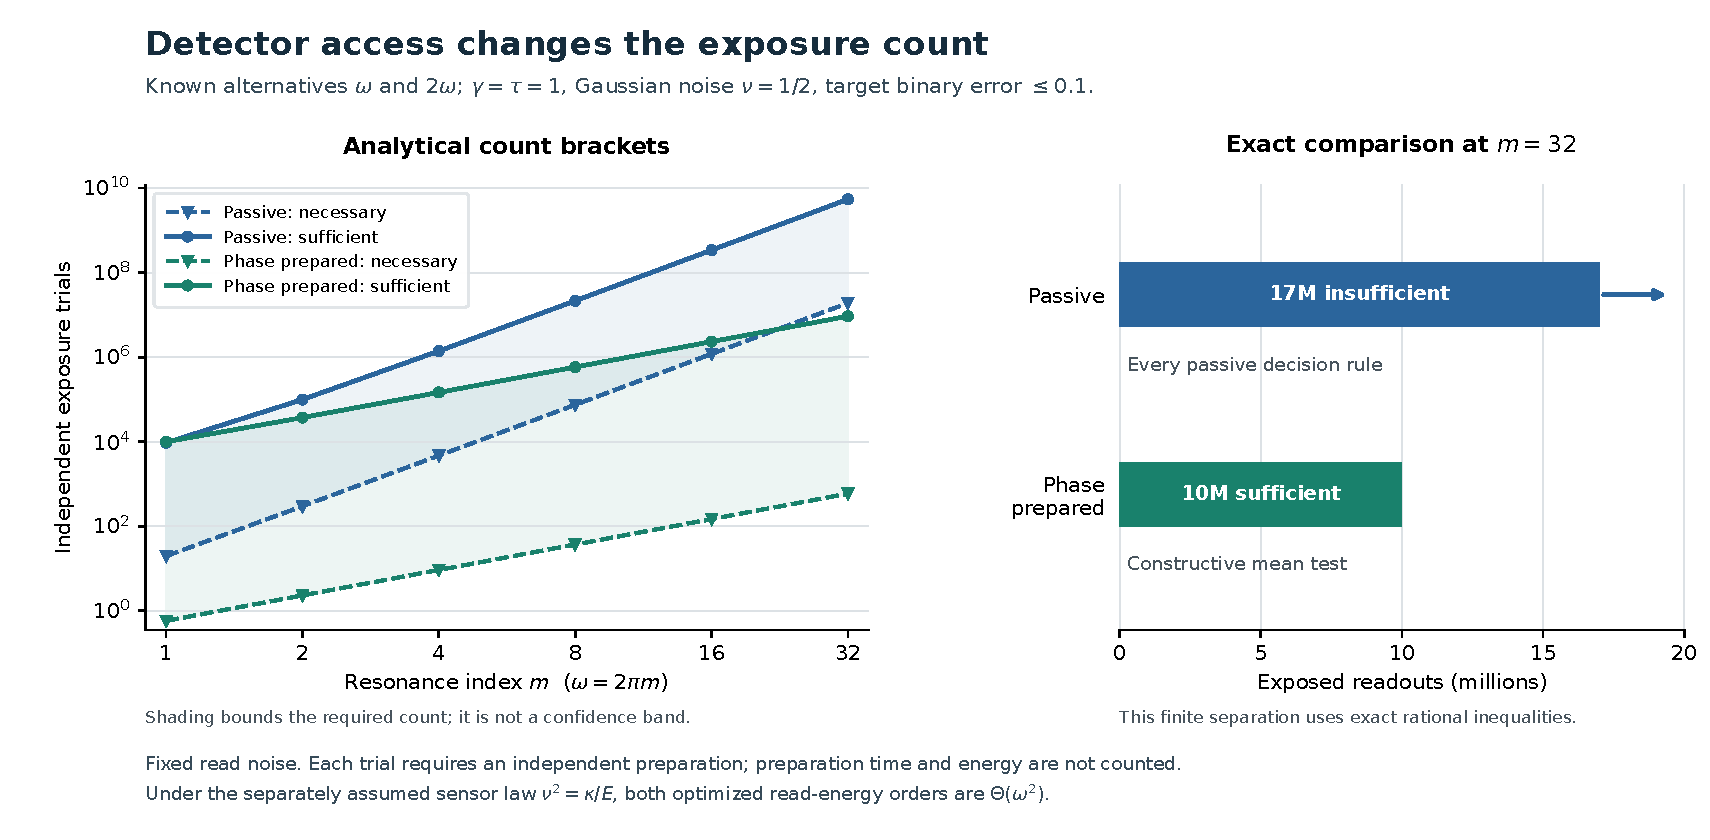
\includegraphics[width=\textwidth]{figures/detector_access.pdf}
 \caption{Analytical exposure-count bounds at fixed read noise. The shaded
 regions bracket the required number of trials; they are not statistical
 confidence bands. The right panel uses the separate exact finite-count
 certificate. Preparation and total apparatus energy are not matched.}
 \label{fig:dg-detector-access}
\end{figure}

The table makes the different fixed-precision count exponents visible.
At the smallest displayed frequency, the prepared constructive guarantee is
slightly more expensive than the passive constructive guarantee; the
asymptotic statement does not promise improvement at every finite parameter.
For a count $n$, both designs acquire $n$ exposed readouts, require $n$
independent preparations and spend $n\tau=n$ units of declared evolution
time. The preparations require different physical access. Their duration,
accuracy and energy have not been assigned a cost here.

These fixed-noise counts do not establish a total-energy advantage.
Under the separately assumed sensor law $\nu_i^2=\kappa/E_i$, optimizing
read precision permits both trial classes to reach the measurement-energy
order $\Theta(\omega^2)$, as proved above. Preparation, reset, driving,
exposure, timing and calibration costs remain separate. No universal
energy--precision law or apparatus performance is inferred from this table.

The implementation retains its exact formulas, 42-digit displays of the real
thresholds, numerical ceilings and source hash in \path{detector/design/results.json}.
Seven deterministic tests check the moments against complex integral formulas,
information-bound constants, constructive error inequalities, asymptotic
orders, precision stability, reproducibility and input guards.

\chapter[Exposure and fixed-rate sampling]{An exact ambiguity after exposure and fixed-rate sampling}
\label{ch:dg-fixed-grid}

A known exposure window does not remove the ambiguity caused by a fixed
sampling interval. This chapter constructs mixing diffusion models whose
complete exposed records agree at every integer time, although their
continuous signal laws and ordinary hidden entropy rates differ. Equality
holds for the entire sampled Gaussian law, so collecting more samples on
the same grid cannot resolve it.

The example uses smooth, uniformly elliptic Ornstein--Uhlenbeck diffusions
on Euclidean space and an unbounded linear detector. Its state space is
\emph{noncompact}. These assumptions differ from the compact, bounded-detector
class used for the earlier sharp minimum theorem. The conclusion concerns
an unbounded range of \emph{actual compatible hidden entropy rates}; no
claim about a change in the minimum compatible entropy follows from this
construction.

\section{An exposed Gaussian oscillator}

Choose units in which the decay rate, exposure width and sampling interval
are all one. Let
\[
 J=\begin{pmatrix}0&-1\\1&0\end{pmatrix},\qquad
 \omega_m=2\pi m,\qquad m\in\{0,1,2,\ldots\}.
\]
For $a>0$, take the stationary Ornstein--Uhlenbeck diffusion in two dimensions
\begin{equation}
 dX_t=(-I+\omega_mJ)X_t\,dt+\sqrt{2a}\,dW_t,
 \qquad X_0\sim N(0,aI).
 \label{eq:dg-ou-model}
\end{equation}
Its diffusion matrix is $aI\succ0$. Its invariant density is Gaussian,
its coefficients are smooth, and its dynamics mix exponentially. If
$Y_t$ is the first coordinate, then
\begin{equation}
 \operatorname{Cov}(Y_0,Y_t)
 =a e^{-|t|}\cos(\omega_mt).
 \label{eq:dg-ou-covariance}
\end{equation}
The measured sequence consists only of the boxcar averages
\begin{equation}
 Z_k=\int_{k-1}^{k}Y_t\,dt,\qquad k\in\mathbb Z.
 \label{eq:dg-ou-readout}
\end{equation}
Exposure is known exactly; no detector noise is needed for the ambiguity.

For a unit-variance oscillator ($a=1$), set
\[
 x_m=(2\pi m)^2,\qquad r=e^{-1},\qquad c_*=2(\cosh1-1).
\]
Direct integration of~\eqref{eq:dg-ou-covariance} gives
\begin{align}
 V_m:=\operatorname{Var}(Z_0)
 &=\frac{2[r+(2-r)x_m]}{(1+x_m)^2},\\
 F_m&=\frac{c_*(1-x_m)}{(1+x_m)^2},\qquad
 \operatorname{Cov}(Z_0,Z_k)=F_m e^{-|k|},\quad k\ne0.
 \label{eq:dg-ou-exposed-moments}
\end{align}
To verify the integration explicitly, put $\lambda_m=-1+i\omega_m$.
For $k\geq1$,
\begin{align*}
 V_m
 &=2\operatorname{Re}
    \frac{e^{\lambda_m}-1-\lambda_m}{\lambda_m^2},\\
 \operatorname{Cov}(Z_0,Z_k)
 &=\operatorname{Re}\left[
 e^{\lambda_m k}
 \frac{e^{\lambda_m}+e^{-\lambda_m}-2}{\lambda_m^2}\right].
\end{align*}
Since $e^{\lambda_m}=e^{-1}$ and
$e^{\lambda_m k}=e^{-k}$ at integer $k$, every member has the same sampled
exponential decay. The variance and its nonzero-lag coefficient retain the
frequency dependence displayed in~\eqref{eq:dg-ou-exposed-moments}.
For general $a$, both quantities are multiplied by $a$.

\section{Matching complete sampled laws}

\begin{theorem}[Known exposure does not identify a fixed-grid diffusion law]
\label{thm:dg-ou-ambiguity}
For every integer $n\geq2$, there are two stationary, exponentially mixing,
smooth uniformly elliptic diffusion models with the following properties:
\begin{enumerate}
 \item their known unit-width boxcar averages have identical complete
       probability laws on the integer grid;
 \item their continuous latent scalar laws differ;
 \item their ordinary hidden entropy rates are $8\pi^2$ and
       $8\pi^2n^2$, respectively.
\end{enumerate}
The first model has two hidden coordinates; the second has four. Their
state spaces are Euclidean and their scalar detectors are linear.
\end{theorem}

\begin{proof}
Let Model A be the $m=1$, $a=1$ oscillator. To construct the second model,
define $R_m=F_m/V_m$. As a function of $x\geq0$,
\[
 R(x)=\frac{c_*}{2}\frac{1-x}{r+(2-r)x},\qquad
 R'(x)=-\frac{c_*}{[r+(2-r)x]^2}<0.
\]
Thus $R_0>R_1>R_n$ whenever $n\geq2$. The coefficients
\begin{equation}
 A_0=\frac{V_1(R_1-R_n)}{(R_0-R_n)V_0},\qquad
 A_n=\frac{V_1(R_0-R_1)}{(R_0-R_n)V_n}
 \label{eq:dg-ou-positive-weights}
\end{equation}
are strictly positive. Their definitions imply the exact identities
\begin{equation}
 A_0V_0+A_nV_n=V_1,\qquad
 A_0F_0+A_nF_n=F_1.
 \label{eq:dg-ou-matching}
\end{equation}
Indeed, the first is the sum of the two complementary interpolation
weights multiplied by $V_1$; the second follows by multiplying them by
$R_0$ and $R_n$.

Let Model B$_n$ consist of two independent oscillators: an $m=0$
oscillator with stationary coordinate variance $A_0$, and an $m=n$
oscillator with stationary coordinate variance $A_n$. Observe the sum
of their first coordinates. The hidden diffusion matrix is
$\operatorname{diag}(A_0I_2,A_nI_2)\succ0$, so this is an admissible smooth
uniformly elliptic Euclidean diffusion. Independence and
\eqref{eq:dg-ou-matching} imply equality of the exposed variance and of
every nonzero-lag covariance with Model A. Both sampled sequences are
centered Gaussian. Every finite-dimensional Gaussian distribution is
determined by its mean and covariance matrix, so \emph{all} finite-dimensional
sampled laws agree, which establishes equality of the entire record laws.

The latent continuous covariance of Model B$_n$ is
\[
 e^{-|t|}\bigl[A_0+A_n\cos(2\pi nt)\bigr],
\]
whereas Model A has covariance $e^{-|t|}\cos(2\pi t)$. These functions
cannot agree: the trigonometric functions at frequencies $0$, $1$ and
$n\geq2$ are linearly independent, and both mixture coefficients are
positive. Hence the continuous scalar laws differ.

Finally, specify ordinary reversal of both hidden coordinates in each
oscillator. The Gaussian stationary density separates the drift in
\eqref{eq:dg-ou-model} into the reversible part $-X$ and current velocity
$v=\omega_mJX$. Therefore
\begin{equation}
 \sigma_m
 =\mathbb E\bigl[(\omega_mJX)^{\mathsf T}(aI)^{-1}
                         (\omega_mJX)\bigr]
 =2\omega_m^2.
 \label{eq:dg-ou-entropy}
\end{equation}
Model A has entropy $8\pi^2$. Entropy is additive for the independent
components of Model B$_n$: the zero-frequency component contributes zero,
and the $m=n$ component contributes $8\pi^2n^2$. This completes the proof.
\end{proof}

For $n=2$, the positive weights are approximately
\[
 A_0=0.0004577350937,\qquad A_2=3.8531460671.
\]
The latent variance is $1$ in Model A and approximately $3.8536038022$
in Model B$_2$. Nevertheless, both exposed integer-grid records have
variance approximately $0.07909835314$ and covariance
$-0.02550729842\,e^{-|k|}$ at nonzero integer lag $k$.
These decimal values illustrate the exact identities; they are not the
basis of the proof.

\section{What the ambiguity establishes}

Letting $n$ increase leaves the complete sampled observation law fixed
while the constructed compatible hidden entropy rates grow without bound.
Every individual model remains finite dimensional and uniformly elliptic,
but there is no common frequency or diffusion-coefficient bound across
the sequence. Such additional prior restrictions would define a different
identification problem. The entropy convention is also substantive:
\eqref{eq:dg-ou-entropy} uses ordinary reversal, not a reversal declaring
one oscillator coordinate odd.

The equality survives every common processing rule for the sampled record.
It also survives adding an independent detector-noise process having the
same specified law under both models. Further samples on the same grid
cannot distinguish the alternatives. Changing the observation times,
retaining the continuous exposed trace, or applying a physical intervention
changes the access contract and is not covered by the equivalence.

There is no conflict with continuous-law recovery under mixing. The
full continuously indexed exposed laws are more informative than their
integer-grid restrictions. The recovery theorem concerns the former;
Theorem~\ref{thm:dg-ou-ambiguity} concerns the latter. Nor does this
construction establish that the compact-class minimum-entropy theorem
extends to these noncompact OU models. Its conclusion is the stated
fixed-grid ambiguity and the absence of a finite upper bound on actual
compatible ordinary entropy within the declared OU family.

The companion implementation evaluates
\eqref{eq:dg-ou-exposed-moments}--\eqref{eq:dg-ou-positive-weights} and
records numerical covariance residuals and entropy values. Five tests
check the exposure formulas against independent integration, positivity
of the mixture coefficients, covariance matching, and entropy scaling,
and reject invalid indices. Those computations diagnose implementation
errors. Exact Gaussian-law equivalence for arbitrarily long records follows
from the analytic argument above; neither a finite covariance checklist
nor simulated data alone would establish it. No laboratory validation or
historical-priority claim is made for this construction.

\chapter{Learning the calibration that an entropy certificate needs}
\label{ch:dc-entry}

An inference method is usable only when its calibration assumptions can be
obtained or justified. The preceding detector chapter established when a
complete observation law retains the ideal diffusion information. A finite
experiment must also account for uncertainty in the detector and in the
diffusion scale. This chapter introduces a construction that does so, together
with a precise obstruction to removing all structural assumptions.

\section{The question answered here}

Suppose a bounded signal is recorded through a shutter and a noisy detector.
Can the same finite records both calibrate its local diffusion scale and
certify positive entropy production, without treating either a fitted scale or
a detector-noise estimate as exact?

The answer developed below is conditional on a specified local geometry:
\[
 |f|\leq1,\qquad \Gamma_f=\gamma(1-f^2),\qquad \gamma>0.
\]
The unknown constant $\gamma$ is estimated. The pointwise functional relation
is a premise. Hidden dimension, hidden drift and stationary density are not
fixed to the circle used in the numerical example. Uniform bounds on the
relevant first and second generator derivatives remain additional premises.
This distinction is substantive: a compact countermodel proves that finite
passive records cannot uniformly certify those global bounds over an
unrestricted smooth diffusion class.

\section{What each part of the experiment supplies}

Repeated detector readings of one exposure estimate powers of its underlying
signal through products of distinct readings. An ordinary power of one noisy
reading does not do this. Conditional independence of the detector
randomizations, a common conditional mean and a bounded output range are the
required noise assumptions; the method does not insert a known read-noise
variance.

A constant reference signal and a timed step reference cover a common
multiplicative gain and the width of a uniform shutter. These are actual
additional reference operations, with their own observations and costs.
They do not establish the local-geometry identity or the generator bounds.
A detector with an unknown offset, changing gain or dependent replica noise
requires a different contract.

Time-separated target records provide a finite-step estimate of the average
local diffusivity. The structural relation then converts this into a covered
bound on $\gamma$. A simultaneous region for fixed measured moments carries
its uncertainty through the entropy calculation. Calibration and testing can
use the same target records because their joint coverage is proved; neither
step is silently treated as certain.

\section{A hierarchy with a finite cost}

The polynomial weights
\[
 w_m(y)=1+y^2+\cdots+y^{2m}
\]
obey $w_m(f)\Gamma_f\leq\gamma$. They replace an inverse local-diffusivity
weight by a finite polynomial that independent replicas can measure. Order
$m$ uses $2m+2$ center readings and one reading at each endpoint. All readings,
including additional replicas, consume physical access.

For the stationary cosine-circle example, the ideal limit at order $m$
recovers the fraction
\[
 1-\frac{\binom{2m+2}{m+1}}{4^{m+1}}
\]
of the exact entropy minimum. This fraction tends to one. The constructive
consistency theorem accounts for an unknown diffusion scale, gain calibration,
finite time steps, shrinking exposure and increasing numerical precision.
It does not claim consistency at a fixed nonzero shutter width or practical
optimality of its conservative acquisition schedule.

The sharp result extends beyond a constant hidden current. Let a reversible
hidden process $Z$ modulate angular drift through $c(Z)$, while the measured
signal remains $\cos\phi$. Within the stated ordinary time-reversal class,
the compatible entropy minimum is exactly $\mathbb E[c(Z)^2]/\gamma$.
It can be positive even when $\mathbb E[c(Z)]=0$, and the complete measured
signal law is time-reversible. Thus mean circulation and observed temporal
asymmetry can both vanish while the observation and its local geometry still
force dissipation. This is an analytic extension; the simulation below uses
constant angular drift.

At a finite budget, more replicas and a higher polynomial order can reduce
performance. The implementation therefore retains the lower orders and
compares them under one simultaneous confidence event. Fixed linear contrasts
preserve correlations between measured moments before concentration; remaining
gain uncertainty is paid through the same covered region. Selecting the
largest covered certificate is justified by that event, rather than by an
uncorrected search through individually valid tests.

\section{How to read the extension}

The calibration-limit chapter explains why additional structure is necessary.
The constructive chapter gives the detector contract, the exposure error
bounds, the joint confidence theorem and the hierarchy. The virtual experiment
then evaluates the actual finite procedure, including its simpler comparator
and unsuccessful regimes. An independent audit checks the proofs and the
implementation; the literature chapter identifies the established inference
methods on which the construction depends.

The numerical experiments use a circle to generate records, but the reported
geometry certificates use the broader stated structural class. A fit that
assumes the complete circle dynamics would answer a different inverse problem.
The mathematical results, simulated observations and requirements for a future
physical experiment retain separate evidence status throughout.

\chapter[Joint detector calibration]{Joint detector calibration and an entropy certificate}
\label{ch:dc-calibration}

Finite detector records need not supply a pointwise volatility estimate in
order to certify dissipation.  Under an explicit structural relation between
the detector coordinate and its local diffusivity, simultaneous moment bounds
can instead calibrate the unknown geometric scale and a polynomial entropy
score.  The construction below accounts for exposure, independent replica
noise and a calibrated detector gain.  It does not infer the structural
relation itself from the records.

\section{Physical and acquisition assumptions}

The hidden process is a stationary smooth uniformly elliptic diffusion on a
smooth compact connected manifold without boundary, with positive smooth
stationary density $\pi$.  Reversal is ordinary hidden-state reversal.  Write
$L=S+A$, $L^\dagger=S-A$, $Af=v\cdot\nabla f$, and
\[
 \Gamma(f,g)=\nabla f^{\mathsf T}D\nabla g,\qquad
 e=v^{\mathsf T}D^{-1}v,\qquad \sigma=\mathbb E_\pi e.
\]
In this convention $d[f(X)]_t=2\Gamma_f(X_t)\,dt$.  For a smooth real
coordinate $f$ with $|f|\le1$, assume the pointwise identity
\begin{equation}
 \Gamma_f(x)=\gamma\bigl(1-f(x)^2\bigr),\qquad
 \gamma>0\text{ unknown and constant}.
 \label{eq:dc-shape}
\end{equation}
Hidden dimension and drift are otherwise unrestricted in the stated class.
An average relation, a stationary marginal or an estimated conditional mean
of $\Gamma_f$ is not a substitute for~\eqref{eq:dc-shape}.  The generator
bounds $M_{1,\pm},M_{2,\pm}$ from the finite-resolution chapter are retained:
\begin{align*}
 \|Lf\|_\infty&\le M_{1,+},&
 \|L^\dagger f\|_\infty&\le M_{1,-},\\
 \|L^2f\|_\infty&\le M_{2,+},&
 \|(L^\dagger)^2f\|_\infty&\le M_{2,-}.
\end{align*}
These are physical calibration assumptions.  Set
$M_*:=\min(M_{1,+},M_{1,-})$ and
$M_{2,*}:=\min(M_{2,+},M_{2,-})$.

Each independent stationary trial has nominal centers $-h,0,h$ and a common
causal uniform exposure
\begin{equation}
 A_t=\frac1\tau\int_{t-\tau}^t f(X_s)\,ds,
 \qquad 0\le\tau\le\tau_U\le h.
 \label{eq:dc-exposure}
\end{equation}
At $\tau=0$, interpret $A_t=f(X_t)$.  Acquire $K=2m+2$ center replicas and
one endpoint readout at each of $-h,h$.  Conditional on the entire hidden
path, all detector randomizations in a trial are independent and each
bounded readout $Z$ has mean $A_t$.  A binary shot with mean $A_t$ is an
example.  Conditional noise independence does not assert independent hidden
states.  Unknown gain is treated separately below.  Repeated powers of a
single noisy readout do not satisfy this replica contract.

\section{An exactly unbiased replica polynomial}

Let $e_k$ be the normalized elementary symmetric polynomial of the $K$
center readouts: the average of all products indexed by distinct
$k$-subsets.  Set $e_0=1$.  The replica assumptions imply
$\mathbb E[e_k\mid X_{\mathbb R}]=A_0^k$.
For fixed $\lambda\in\mathbb R$, put
\begin{align}
 b&=1-\lambda h,&
 \beta_g&=\frac h4(M_{2,+}+M_{2,-}),\\
 \beta_K&=\frac h2(M_{1,-}M_{2,+}+M_{1,+}M_{2,-}),&
 \beta&=2|\lambda|\beta_g+\beta_K.
 \label{eq:dc-beta}
\end{align}
Define the record score
\begin{equation}
 T_m=\frac1{h^2}\sum_{j=0}^m
 \left[-Z_-Z_+e_{2j}
       +b(Z_-+Z_+)e_{2j+1}-b^2e_{2j+2}\right]
       -\beta\sum_{j=0}^m e_{2j}.
 \label{eq:dc-replica-score}
\end{equation}
Its expectation is exactly the displayed polynomial in $A_-,A_0,A_+$.
Write $T_m^{\rm ideal}$ for that polynomial evaluated at
$Y_t=f(X_t)$ instead.

\begin{proposition}[Ideal polynomial inequality]
Under~\eqref{eq:dc-shape},
\begin{equation}
 \mathbb E T_m^{\rm ideal}\le\gamma\sigma.
 \label{eq:dc-polynomial-physical}
\end{equation}
\end{proposition}
\begin{proof}
Set $w_m(y)=\sum_{j=0}^m y^{2j}$ and $q(y)=-\lambda y$.  The uncorrected
ideal polynomial is
\[
 -w_m(Y_0)
 \left(q(Y_0)-\frac{Y_h-Y_0}{h}\right)
 \left(q(Y_0)-\frac{Y_{-h}-Y_0}{h}\right).
\]
The two-sided semigroup bounds in the finite-resolution chapter control its
conditional time-step bias by $2|q|\beta_g+\beta_K\le\beta$.  Conditional on
the complete center state, the corrected expectation is therefore at most
\[
 w_m(f)\{2qSf-q^2-(Sf)^2+(Af)^2\}
 =w_m(f)\{(Af)^2-(q-Sf)^2\}.
\]
Since $(Af)^2\le\Gamma_f e$ and
$w_m(f)\Gamma_f=\gamma(1-f^{2m+2})\le\gamma$, integration proves the claim.
The argument does not clip individual records or intermediate expectations.
\end{proof}

\section{A multitime moment bound for exposure}

\begin{lemma}[Bidirectional gap derivative]
For the stationary ordered moment
$F(t_1,\ldots,t_d)=\mathbb E\prod_i f(X_{t_i})$, its derivative in gap $j$
satisfies
\begin{equation}
 \left|\partial_{t_{j+1}-t_j}F\right|
 \le a_{d,j}:=
 \min\{j^2M_{1,-},(d-j)^2M_{1,+}\},\qquad 1\le j<d.
 \label{eq:dc-gap}
\end{equation}
The assertion includes one-sided limits at coincident times.
\end{lemma}
\begin{proof}
A backward semigroup word $g$ containing $k$ factors $f$ obeys
$\|g\|_\infty\le1$ and $\|Lg\|_{L^1(\pi)}\le k^2M_{1,+}$.
For the induction, semigroup application preserves this bound by stationary
$L^1$ contraction and commutation with $L$.  Multiplication uses
\begin{gather*}
 L(fg)=fLg+gLf+2\Gamma(f,g),\\
 \mathbb E\Gamma_f=-\mathbb E fLf\le M_{1,+},\qquad
 \mathbb E\Gamma_g=-\mathbb E gLg\le\|Lg\|_1.
\end{gather*}
The Cauchy inequality for $\Gamma$ gives the new bound
$B+M_{1,+}+2\sqrt{BM_{1,+}}$ when the old bound is $B$; if
$B\le(k-1)^2M_{1,+}$, the result is at most $k^2M_{1,+}$.
At a gap, the conditional product of preceding factors has absolute value
at most one.  Differentiating the suffix and integrating its generator in
$L^1(\pi)$ yields the $(d-j)^2M_{1,+}$ bound.  Applying the same argument
under stationary time reversal gives $j^2M_{1,-}$.  Smooth compactness
justifies the generator identities and differentiation.
\end{proof}

For arbitrary causal exposure supported in $[t_i-\tau,t_i]$, sorted
displacements from the nominal ordered times lie in $[-\tau,0]$, so each
gap changes by at most $\tau$.  Consequently a degree-$d$ product changes by
at most
\begin{equation}
 \tau\sum_{j=1}^{d-1}a_{d,j}.
 \label{eq:dc-support-blur}
\end{equation}
Products of exposure averages are integrals over auxiliary exposure times;
these integration variables do not imply independence of signal values.

Common uniform boxes give explicit sharper constants.  Suppose the nominal
windows do not overlap and have chronological multiplicities
$(p_1,\ldots,p_r)$, deleting zero entries, with $d=\sum_i p_i$.  Define
$B(p_1,\ldots,p_r)$ by summing the following contributions at each global
prefix $k$.  An internal gap of a cluster with $p$ factors contributes
\begin{equation}
 \frac{a_{d,k}}{p+1}.
 \label{eq:dc-internal-spacing}
\end{equation}
A gap between consecutive clusters with $p$ and $q$ factors contributes
\begin{equation}
 a_{d,k}\left[1-\frac1{p+1}-\frac1{q+1}
                  +\frac{2p!q!}{(p+q+1)!}\right].
 \label{eq:dc-cross-spacing}
\end{equation}
The resulting blur radius is $\tau_U B(p_1,\ldots,p_r)$; degrees zero and
one have radius zero.  To verify the formula, internal uniform order-statistic
spacings have mean $1/(p+1)$.  A cross-gap displacement divided by $\tau$ is
$U_{\min,q}-U_{\max,p}$.  Its positive part has expectation
\[
 \int_0^1t^p(1-t)^q\,dt=\frac{p!q!}{(p+q+1)!},
\]
while the mean of its negative is
$1-1/(p+1)-1/(q+1)$.  This yields its expected absolute value in
\eqref{eq:dc-cross-spacing}.  Integrate~\eqref{eq:dc-gap} along the segment
between the two nonnegative gap vectors and then average.

\section{Calibrating the geometric scale}

Let
\[
 C(t)=\mathbb E[Y_0Y_t],\quad D_0=\mathbb E A_0^2,\quad
 D_h=\mathbb E[A_0A_h],\quad q_0=\mathbb E\Gamma_f.
\]
Stationarity implies $C(-t)=C(t)$, $C'(0+)=-q_0$, $q_0\le M_*$ and
$|C''(t)|\le M_{2,*}$ for $t\ge0$, with a right derivative at zero.  Hence
\begin{align}
 0\le C(0)-D_0&\le\delta_0:=\frac{M_*\tau_U}{3},\\
 |D_h-C(h)|&\le\delta_h:=\frac{M_{2,*}\tau_U^2}{12}.
 \label{eq:dc-covariance-blur}
\end{align}
The first bound uses $C(t)\le C(0)$, the Lipschitz constant $M_*$ and
$\mathbb E|U-V|=\tau/3$ for two uniform exposure offsets.  The second uses
their centered difference, whose variance is $\tau^2/6$, in the Taylor
remainder; $h\ge\tau$ prevents passage through the covariance cusp.  The
same bound holds at $2h$.  A more precise identity is
$D_0=C(0)-q_0\tau/3+R_0$, with $|R_0|\le M_{2,*}\tau^2/12$; the displayed
bound avoids an unknown $q_0$ in the calibration envelope.

Write $\mathcal D(p_1,\ldots,p_r)$ for either valid general blur radius
above, optionally replacing a degree-two radius by $\delta_0$ for one window
and by $\delta_h$ for distinct windows separated by at least $h$.  Define
\begin{align}
 \delta_N={}&\frac1{h^2}\sum_{j=0}^m
 \bigl\{\mathcal D(1,2j,1)
 +|b|[\mathcal D(1,2j+1)+\mathcal D(2j+1,1)]
 +b^2\mathcal D(2j+2)\bigr\}\\
 &\quad+\beta\sum_{j=0}^m\mathcal D(2j).
 \label{eq:dc-score-blur}
\end{align}
Delete zero clusters before evaluation.  The last term accounts for blur of
the bias-correction moments.  The two cross terms need not have identical
bounds when the forward and adjoint caps differ.

The following three population quantities now have compatible directions:
\begin{align}
 P&=\mathbb ET_m-\delta_N\le\gamma\sigma,\\
 \overline A&=1-D_0-\delta_0\le A_{\rm true}:=1-C(0),\\
 \overline H&=\frac{D_0-D_h+\delta_0+\delta_h}{h}
                     +\frac{M_{2,*}h}{2}
                 \ge\gamma A_{\rm true}.
 \label{eq:dc-three-population}
\end{align}
The last inequality follows from
$|C(0)-C(h)-hq_0|\le M_{2,*}h^2/2$ and the exact relation
$q_0=\gamma(1-C(0))$.  This step uses neither an arcsine marginal nor a
local-volatility estimate.

\section{A simultaneous finite-record certificate}

\begin{theorem}[Joint geometry and score calibration]
Assume simultaneous bounds $p\le P$, $a\le\overline A$ and
$u\ge\overline H$ hold with probability at least $1-\alpha$ for the
declared acquisition.  Set
\begin{equation}
 \widehat L=
 \begin{cases}
 [p]_+[a]_+/u,&u>0,\\
 0,&u\le0,
 \end{cases}
 \label{eq:dc-certificate}
\end{equation}
marking the latter case inconclusive.  Then
$\Pr(\sigma\ge\widehat L)\ge1-\alpha$.  On the same confidence event, if
$a>0$, then $\gamma\le u/a$.
\end{theorem}
\begin{proof}
If $p,a>0$, then $A_{\rm true}>0$ and
$u\ge\gamma A_{\rm true}>0$.  Therefore
$pa/u\le\sigma a/A_{\rm true}\le\sigma$.  Otherwise the displayed lower
bound is zero.  The geometric upper bound follows from
$u\ge\gamma A_{\rm true}\ge\gamma a$.
\end{proof}

One construction covers the means of $T_m$, $e_2$ and
$(Z_-+Z_+)e_1/2$ simultaneously using the same independent trials.  Their
population means are respectively $\mathbb ET_m,D_0,D_h$.  Interval
arithmetic supplies the required lower and upper endpoints.  Unconditional
bounded-mean concentration for each statistic, followed by a declared union
bound, remains valid when the statistics share records.  There is no need
to split data merely because the geometric scale and the entropy score are
calibrated together.

For $|Z|\le B$, $|e_k|\le B^k$, so valid finite score ranges follow directly.
Hoeffding or a valid empirical-Bernstein inequality supplies the mean
intervals.  Numerical endpoints require outward enclosure.  A variance
estimate cannot be substituted into a theorem requiring a known variance.
Selecting $m$ or $\lambda$ from the same records is valid only if the
underlying moment region or a finite-family confidence event covers that
selection.  Applying an ordinary iid score inequality after an uncovered
coefficient selection would not establish the theorem's premise.

\section{Unknown detector gain and a physical reference protocol}

Suppose a raw bounded readout $R$ has mean $\kappa A_t$ conditional on the
hidden path, with unknown common constant $\kappa>0$.  A raw degree-$d$
product has mean $\kappa^d$ times its exposed moment.  Cover its raw mean and
project that interval over a simultaneously covered positive gain region;
this is different from inserting an estimated gain as if exact.
In the formulas of this gain-calibration section and the raw-contrast
projection below, $e_k$ denotes the elementary polynomial of the raw center
readouts $R$, before gain correction.

For example, the complete raw contrast
\begin{equation}
 S_j=\frac1{h^2}\left[-R_-R_+e_{2j}
       +b(R_-+R_+)e_{2j+1}-b^2e_{2j+2}\right]
 \label{eq:dc-gain-contrast}
\end{equation}
has homogeneous degree $2j+2$.  Its mean interval can be divided by
$\kappa^{2j+2}$ while retaining cancellations within the contrast.  The
degree-$2j$ bias-correction means are handled separately.  Signed endpoints
must be minimized or maximized over the gain interval: dividing every
endpoint by its lower gain is invalid for negative means.  A full joint
region may preserve the common gain across degrees; rectangular projection
is conservative.  If the gain region reaches zero, finite inverse bounds
may be unavailable and the procedure can abstain.

A concrete bounded reference protocol can calibrate both gain and exposure.
Feed the same detector a known constant signal one, whose mean readout is
$\kappa$.  Also feed a known step from zero to one at time zero.  If a
coarse metrological bracket permits a fixed reference time
$0<s<\tau_{\min}\le\tau$, the step's mean readout is
\begin{equation}
 p_{\rm step}=\kappa s/\tau.
 \label{eq:dc-step}
\end{equation}
Simultaneous bounded-mean confidence intervals yield the joint constraints
\[
 \kappa\in[\kappa_L,\kappa_U],\qquad
 p_{\rm step}\in[p_L,p_U],\qquad p_{\rm step}\tau=\kappa s.
\]
When $p_L>0$, a conservative exposure interval is
\begin{equation}
 \left[\frac{\kappa_Ls}{p_U},\frac{\kappa_Us}{p_L}\right]
 \label{eq:dc-shutter-region}
\end{equation}
intersected with the coarse bracket.  Without the ramp condition the correct
response is $\kappa\min(1,s/\tau)$, and that relation must be retained.
An empty region is an inconclusive/model-check flag.  A nonpositive lower
step mean can leave the exposure upper bound inconclusive.

These references require a known input shape, a known time origin and common
detector response between reference and target.  They do not validate
\eqref{eq:dc-shape} or the generator caps.  Cover all raw target and reference
means with one declared error allocation.  Dependence among statistics from
the same trials is harmless to a union bound; independence across the trials
used by each concentration inequality is still required.  Adaptive reference
design requires its own valid confidence argument.

\section{Retaining covariance before nuisance projection}

Intervals for separate polynomial components can discard useful cancellations.
A predetermined raw contrast can retain those cancellations before concentration,
while still allowing an uncertain gain afterward.  Choose a nominal
$\kappa_0>0$ as a predeclared fixed design constant, or using a pilot
independent of the inference records, and include in the same covered mean
vector, all $S_j$, the required $e_{2j}$, the calibration contrast, and
\begin{equation}
 R_\ell=\sum_{j=0}^{\ell}\frac{S_j}{\kappa_0^{2j+2}},
 \qquad 0\le\ell\le m.
 \label{eq:dc-predetermined-contrast}
\end{equation}
Here the $S_j$ include the $h^{-2}$ factor in
\eqref{eq:dc-gain-contrast}.  A confidence interval for $\mathbb ER_\ell$
is computed from its actual record variance or range, not by summing the
individual $S_j$ margins.  This is the established principle of concentrating
a fixed linear contrast before projecting nuisance uncertainty.

Suppose $\mathbb ES_j\in[L_j,U_j]$ and
$\mathbb ER_\ell\ge L_{R_\ell}$ on the common confidence event.  For
$d_j=2j+2$, define
\[
 I_j=[\kappa_U^{-d_j}-\kappa_0^{-d_j},
       \kappa_L^{-d_j}-\kappa_0^{-d_j}],\qquad
 c_j=\min\{xy:x\in\partial I_j,\ y\in\{L_j,U_j\}\}.
\]
The four-corner minimum is valid because a bilinear function on a rectangle
attains its extrema at corners.  For every gain in the covered interval,
\begin{equation}
 \sum_{j=0}^{\ell}\frac{\mathbb ES_j}{\kappa^{2j+2}}
 =\mathbb ER_\ell+
   \sum_{j=0}^{\ell}(\kappa^{-d_j}-\kappa_0^{-d_j})\mathbb ES_j
 \ge L_{R_\ell}+\sum_{j=0}^{\ell}c_j.
 \label{eq:dc-correlation-projection}
\end{equation}
Subtract the covered upper bound on
$\beta\sum_{j=0}^{\ell}\mathbb E e_{2j}/\kappa^{2j}$ and the appropriate
$\delta_N$ to obtain a lower bound for $P_\ell$.  The maximum of this bound
and the componentwise lower bound remains valid on the same event.  All
prefixes $\ell\le m$ use the same $K=2m+2$ genuine replicas: their elementary
averages remain unbiased.  Once the common confidence vector covers every
contrast actually used, choosing the largest certificate across these
prefixes spends no further error probability.  Adding an uncovered contrast
after inspecting the data would require additional justification.

\section{An endpoint entropy comparison}

The order-zero raw contrast also provides a comparison that does not require
the structural identity~\eqref{eq:dc-shape}.  Keep the stationary ordinary
diffusion and detector assumptions and let $0\le b\le1$.  Suppose the common
confidence event gives $s$ below the ideal, gain-corrected and blur-corrected
mean
\begin{equation}
 N_0=\frac{2bC(h)-C(2h)-b^2C(0)}{h^2}.
 \label{eq:dc-endpoint-target}
\end{equation}
This endpoint comparison subtracts the raw order-zero blur radius, but not
the $\beta$ penalty used by the derivative-based entropy score.  Then
\begin{equation}
 \sigma\ge\frac{2h^3[s]_+^2}{(2b+\sqrt2)^2}.
 \label{eq:dc-endpoint-baseline}
\end{equation}
This is the earlier reversible-support and entropy-bridge construction,
expressed in the current covariance normalization.

To check constants, compare $L$ with $S=(L+L^\dagger)/2$ using the same
stationary density, diffusion tensor and coordinate.  The diffusion
Girsanov identity gives
$D(P_L^{[0,t]}\Vert P_S^{[0,t]})=\sigma t/4$.  Pinsker and the bounded
endpoint product yield
$|C_L(t)-C_S(t)|\le\sqrt{\sigma t/2}$.  The zero-lag moments agree exactly,
and reversibility gives
\[
 2bC_S(h)-C_S(2h)-b^2C_S(0)
   =-\|(e^{hS}-bI)f\|_{L^2(\pi)}^2\le0.
\]
It follows that $h^2[N_0]_+\le(2b+\sqrt2)\sqrt{\sigma h/2}$, which proves
\eqref{eq:dc-endpoint-baseline}.  Exposure errors must be removed before
using the ideal zero-lag cancellation.  Both entropy bounds can be reported
on the same simultaneous confidence event.  Their difference then reflects
different physical inequalities, with detector and calibration access held
fixed, rather than a comparison against an uncorrected estimator.

\section[Sharp limiting hierarchy]{A sharp limiting hierarchy with unknown scale}

For the stationary circle
$d\phi=\omega\,dt+\sqrt{2\gamma}\,dW$ and $f=\cos\phi$, one has
$Sf=-\gamma f$ and $(Af)^2=\omega^2(1-f^2)$.  The zero-step weighted target
divided by $\gamma$ is exactly
\begin{equation}
 J_m(\lambda)=\frac{\omega^2}{\gamma}
       \bigl(1-\mathbb EY^{2m+2}\bigr)
 -\frac{(\lambda-\gamma)^2}{\gamma}
       \mathbb E[w_m(Y)Y^2].
 \label{eq:dc-hierarchy}
\end{equation}
For $\lambda=\gamma$, this increases to the attained compatible-law minimum
$\sigma=\omega^2/\gamma$, since
\[
 \mathbb EY^{2m+2}
 =\frac{\binom{2m+2}{m+1}}{4^{m+1}}=O(m^{-1/2}).
\]
A grid point with $|\lambda-\gamma|\le\eta$ loses at most
$(m+1)\eta^2/\gamma$.  A deterministic finite grid with simultaneous
coverage therefore permits choosing the largest certified lower bound
without knowing $\gamma$.  Independently, $u/a$ converges to $\gamma$ as
the moment error, exposure error divided by $h$, and $h$ vanish with
$C(0)<1$.

For clarity, a conservative sufficient sequence makes the statement
constructive and removes the need for an oracle choice of $\lambda$.  Use
raw target and reference readouts bounded by one, as in the binary detector
example.  Fix positive parameter envelopes for the circle and valid resulting generator
caps.  Suppose a known integer $B\ge0$ obeys
$\kappa\ge\kappa_{\min}\ge2^{-B}$.  In a fixed time unit, at stage $k$ take
\begin{equation}
 \begin{gathered}
 m=k,\qquad h_k=2^{-k},\qquad \tau_k\le2^{-4k},\\
 K_k=2k+2,\qquad n_k=n_{{\rm ref},k}=2^{(8B+16)k}.
 \end{gathered}
 \label{eq:dc-consistency-schedule}
\end{equation}
Use the finite grid $[0,k]\cap2^{-k}\mathbb Z$ for $\lambda$.  References
use a known coarse shutter bracket shrinking at the stated exposure scale,
so their upper exposure bound also has that order.  Allocate a fixed total
error probability over all covered means and grid scores, or a summable
stagewise allocation.  Eventually the grid contains a point within $2^{-k}$
of the fixed true $\gamma$.

The raw score ranges are at most a polynomial in $k$ times $2^{2k}$.
Correcting degree at most $2k+2$ for gain multiplies interval widths by at
most $2^{2B(k+1)}$.  A bounded-mean radius with the declared sample size is
therefore at most a polynomial in $k$ times $2^{-(2B+6)k}$; the logarithm
of the finite-family size is $O(k)$.  Gain uncertainty has the same
vanishing order up to fixed and polynomial factors, by differentiating
$\kappa^{-d}$ on the known positive gain interval.  The calibration
reference count is included in~\eqref{eq:dc-consistency-schedule}.

The generic exposure bound gives
$O(k^4\tau_k/h_k^2)=O(k^4 2^{-2k})$ for raw-score blur.  The bias-correction
blur is smaller.  Uniformly over the finite grid, the finite-step penalty
is $O(k^2 2^{-k})$.  The nearest grid point loses $O(k4^{-k})$ in
\eqref{eq:dc-hierarchy}, while the gamma upper bound converges to the true
$\gamma$.  Direct uniform concentration around the covered means now gives
\begin{equation}
 \begin{gathered}
 \max_{\lambda\text{ on the grid}}\widehat L_k
       \longrightarrow\sigma\quad\text{in probability},\\
 \sigma-\max\widehat L_k
       =O_{\mathbb P}(k^{-1/2})
       =O_{\mathbb P}((\log n_k)^{-1/2}).
 \end{gathered}
 \label{eq:dc-consistency}
\end{equation}
In the last expression the difference is signed; the stochastic error is
smaller than the displayed order.  This rate is a conservative sufficient
rate, not a minimax assertion.  Direct concentration proves convergence
even at a fixed advertised confidence level; coverage alone would not.

Numerical enclosure error must also vanish after degree and time-step
amplification.  For example, carrying certified elementary-operation
enclosures to $k^2+(4B+12)k$ binary digits is ample for the finite algebraic
construction just described.  This includes refining any logarithm-series
truncation and square-root enclosure, rather than only rounding a fixed
approximation to more digits.  An implementation that retains a fixed
absolute rounding floor remains a valid finite-stage certificate, but its
unchanged output is not asserted to satisfy~\eqref{eq:dc-consistency}.

This is an existence construction with increasing physical access, not a
practical acquisition recommendation.  It requires shrinking exposure,
increasing replica access and reference measurements.  Fixed positive
exposure is not removed by this finite-difference argument.  Reset and
reference energies remain separate acquisition costs.

\section{Sharpness with an unobserved stochastic drive}

The sharp hierarchy is not confined to constant angular drift.  Let $Z$ be
any smooth reversible uniformly elliptic diffusion on a compact connected
manifold without boundary, with generator $L_Z$ and positive smooth
stationary density $\pi_Z$.  For a smooth real function $c$ on that manifold,
consider the joint generator
\begin{equation}
 L=\gamma\partial_\phi^2+c(z)\partial_\phi+L_Z,
 \qquad \phi\in\mathbb S^1,\qquad \gamma>0.
 \label{eq:dc-modulated-generator}
\end{equation}
All coordinates are subject to ordinary, even-variable reversal.  The
stationary measure is $(d\phi/2\pi)\pi_Z(dz)$: the angular drift is
divergence-free with respect to the uniform angular measure, and $L_Z$
preserves $\pi_Z$.  The diffusion tensor is block diagonal with angular
entry $\gamma$.  Thus
\begin{equation}
 S=\gamma\partial_\phi^2+L_Z,\qquad
 A=c(z)\partial_\phi,\qquad
 \sigma=\frac{\mathbb E_{\pi_Z}c^2}{\gamma}.
 \label{eq:dc-modulated-entropy}
\end{equation}

\begin{proposition}[Sharp minimum under reversible hidden modulation]
For $f(\phi,z)=\cos\phi$, the full stationary scalar observation law is
time-reversible.  Nevertheless its minimum compatible entropy over the
ordinary compact hidden-diffusion class of the observed-geometry theorem is
exactly $\mathbb E_{\pi_Z}c^2/\gamma$.  The actual joint diffusion attains
that value.  The finite polynomial hierarchy has the same sharp limit and
the same ideal formula~\eqref{eq:dc-hierarchy}, with
$\omega^2$ replaced by $\mathbb E_{\pi_Z}c^2$.
\end{proposition}
\begin{proof}
Direct computation gives
\[
 \Gamma_f=\gamma(1-f^2),\qquad Sf=-\gamma f,\qquad
 Af=-c(z)\sin\phi.
\]
At stationarity $Z$ and $\phi$ are independent, and
$U=(f,\Gamma_f)$ contains only $Y=f$.  The conditional quantities in the
population observed-geometry theorem therefore satisfy
\begin{align*}
 g(Y)&=-\gamma Y,\\
 K(Y)&=\gamma^2Y^2
       -\mathbb E_{\pi_Z}c^2\,(1-Y^2).
\end{align*}
The integrated conditional bound is
\[
 \mathbb E\left[
 \frac{[g(Y)^2-K(Y)]_+}{\gamma(1-Y^2)}
       \boldsymbol 1_{\{|Y|<1\}}\right]
 =\frac{\mathbb E_{\pi_Z}c^2}{\gamma}.
\]
The excluded endpoints have zero stationary probability.  This functional is
fixed by the ideal continuous observation law, so it bounds every compatible
ordinary hidden diffusion from below.  Equation~\eqref{eq:dc-modulated-entropy}
provides a realization attaining it.

For reversibility of the observation, the reflection
$\mathcal R(\phi,z)=(-\phi,z)$ preserves the stationary measure, fixes $f$
and conjugates $L$ to $L^\dagger$.  Applying this reflection to the reversed
stationary hidden path thus restores its forward law without changing any
detector values.  All finite-dimensional distributions of $Y$ agree with
their time reverses.  Finally, stationarity and independence yield
\begin{align*}
 \frac1\gamma\mathbb E\left[
 w_m(Y)\{(Af)^2-(-\lambda Y-Sf)^2\}\right]
 &={}\frac{\mathbb E c^2}{\gamma}
       (1-\mathbb EY^{2m+2})\\
 &\quad-\frac{(\lambda-\gamma)^2}{\gamma}
       \mathbb E[w_m(Y)Y^2],
\end{align*}
which proves the hierarchy assertion.
\end{proof}

The same sufficient acquisition and precision schedule applies under valid
uniform generator and positive-gain envelopes: the stationary arcsine
marginal and ideal hierarchy formula are unchanged, while the finite-lag
and exposure bounds already hold for the general hidden class.

The generator calibration can also be written explicitly.  Let
$C=\|c\|_\infty$ and $G=\|L_Zc\|_\infty$.  Then
\begin{align}
 Lf&=-\gamma\cos\phi-c\sin\phi,\\
 L^2f&=(\gamma^2-c^2)\cos\phi
                  +(2\gamma c-L_Zc)\sin\phi.
 \label{eq:dc-modulated-caps}
\end{align}
The adjoint formulas reverse the sine terms.  Both first-order norms equal
$\sqrt{\gamma^2+C^2}$, and both second-order norms equal
\[
 \sup_z\sqrt{(\gamma^2-c(z)^2)^2+
                       (2\gamma c(z)-L_Zc(z))^2}.
\]
The simple choices $M_{1,\pm}=\gamma+C$ and
$M_{2,\pm}=(\gamma+C)^2+G$ consequently suffice.  For unknown parameters,
calibrated upper envelopes for these expressions are required, just as in
the main finite certificate; the records do not automatically certify them.

For an explicit zero-mean example take a second angle $z$,
$L_Z=\eta\partial_z^2$ with $\eta>0$, and $c(z)=\varepsilon\cos z$.
Then
\begin{equation}
 \begin{gathered}
 \mathbb E c=0,\qquad
 \sigma=\frac{\varepsilon^2}{2\gamma},\qquad
 M_{1,\pm}=\sqrt{\gamma^2+\varepsilon^2},\\
 M_{2,\pm}=\sqrt{(\gamma^2-\varepsilon^2)^2
                            +(2\gamma+\eta)^2\varepsilon^2}.
 \end{gathered}
 \label{eq:dc-zero-mean-drive}
\end{equation}
The last identity follows by maximizing the squared norm over
$c^2\in[0,\varepsilon^2]$; its derivative in $c^2$ is positive.  Mean angular
current vanishes, but nonzero conditional angular currents remain and the
ordinary-reversal entropy minimum is positive when $\varepsilon\ne0$.
This is an analytically verified family, not an additional simulation or
physical experiment.  Interpreting a hidden coordinate as odd under
physical reversal changes the admissible class and can change the entropy
target; that interpretation is not included here.

\section{Scope and failure modes}

The theorem calibrates a scale in a declared pointwise geometry.  It does not
learn arbitrary hidden diffusivity or global generator suprema from a finite
record.  Rare-state countermodels obstruct that stronger inference.  A
false structural identity, correlated detector randomization, an altered
reference response, nonstationary target records or uncharged trial
dependence invalidates the certificate.  A single noisy center value cannot
replace the distinct replicas.

Replica inference, confidence-region inversion and the semigroup and
Dirichlet identities used here are established tools.  The result assembled
here is their explicit finite-sample propagation into this entropy
functional and its polynomial limiting hierarchy.  The record count,
replica channels, references, exposure and evolution time are acquisition
resources.  Total energy requires a separate calibrated sensor and preparation
model; it is not inferred from the sample count.

\chapter[Limits of empirical calibration]{Why empirical averages cannot certify global calibration}
\label{ch:dc-calibration-limits}

A finite record can estimate the local fluctuations it samples without
controlling fluctuations in every hidden state. The distinction matters
when an entropy certificate requires a pointwise diffusivity envelope or
a supremum bound on generator derivatives. Smoothness of each possible
model, by itself, does not provide the common numerical constants needed
for that extrapolation.

This chapter proves a precise obstruction. Over a class of smooth compact
diffusions, any uniformly covered upper confidence bound for global local
diffusivity must be infinite with probability at least its nominal coverage,
even under a benign reference process. The result holds with a bounded
detector, known uniform stationary density, fixed hidden dimension, a common
ellipticity lower bound, and a common mixing gap. It even holds when the
complete hidden trajectory is observed continuously and without noise.
Two further constructions separate the regularity assumptions: an upper
bound on diffusivity does not bound $Lf$, and upper bounds on both
diffusivity and $Lf$ do not bound $L^2f$.

These are statements about global or stationary essential suprema.
They do not deny that an ideal continuous path determines local volatility
along that path. Every model constructed below is reversible and has zero
ordinary entropy production; no change in an ideal-law entropy minimum
is asserted.

\section{A compact diffusion with an arbitrarily high rare bump}

Let $(x,z)$ lie on the torus $\mathbb T^4=(\mathbb R/2\pi\mathbb Z)^4$,
where $z$ has three coordinates. Near the origin in its fundamental cube
$[-\pi,\pi]^3$, use the Euclidean norm $|z|$. Choose a smooth radial profile
$b$ satisfying
\[
 0\leq b\leq1,\qquad b(s)=1\ (0\leq s\leq\tfrac12),\qquad
 b(s)=0\ (s\geq1).
\]
One explicit choice on $1/2<s<1$ is
\begin{equation}
 b(s)=\frac{h(1-s)}{h(1-s)+h(s-1/2)},\qquad
 h(t)=\begin{cases}e^{-1/t},&t>0,\\0,&t\leq0.\end{cases}
 \label{eq:dc-bump-profile}
\end{equation}
Together with its constant pieces this profile is $C^\infty$. Being
constant near zero also makes $b(|z|/r)$ smooth at the origin.

For $M\geq1$ and $0<r\leq1/2$, set
\begin{equation}
 \begin{split}
 d_{M,r}(z)&=1+(M-1)b(|z|/r),\\
 L_{M,r}&=d_{M,r}(z)\partial_x^2+\Delta_z,\qquad
 D_{M,r}=\operatorname{diag}(d_{M,r},1,1,1),\\
 f(x,z)&=\cos x.
 \end{split}
 \label{eq:dc-rare-model}
\end{equation}
The bump is supported strictly inside the fundamental cube, so it extends
smoothly and periodically. In It\^o form the process satisfies
\[
 dx_t=\sqrt{2d_{M,r}(z_t)}\,dW_t^x,
 \qquad dz_t=\sqrt2\,dW_t^z,
\]
with independent Brownian components and coordinates taken modulo $2\pi$.
The detector lies in $[-1,1]$.

The normalized uniform density $\pi=(2\pi)^{-4}$ is stationary. Although
$d$ depends on $z$, its only nonconstant tensor entry is the $xx$ entry,
so $L=\operatorname{div}(D\nabla)$ and $L$ is self-adjoint in $L^2(\pi)$.
Each model is smooth, connected, compact and uniformly elliptic, with the
common lower bound $D\succeq I$. Its stationary current vanishes, giving
ordinary entropy rate $\sigma=0$.

The mixing gap does not deteriorate with the bump. For every smooth
mean-zero function $g$, the torus Poincar\'e inequality gives
\begin{equation}
 -\langle g,Lg\rangle_\pi
 =\mathbb E_\pi[d|\partial_xg|^2+|\nabla_zg|^2]
 \geq\mathbb E_\pi[|\nabla g|^2]
 \geq\mathbb E_\pi[g^2].
 \label{eq:dc-common-gap}
\end{equation}
Thus the $L^2$ spectral gap is at least one, and the mean-zero semigroup
contracts at least as fast as $e^{-t}$. The construction does not rely on
metastability or a disappearing lower ellipticity constant.

For the detector in~\eqref{eq:dc-rare-model}, direct calculation yields
\begin{align}
 \Gamma_f&=\nabla f^{\mathsf T}D\nabla f=d_{M,r}\sin^2x,\\
 Lf&=-d_{M,r}\cos x,\\
 L^2f&=(d_{M,r}^2-\Delta_zd_{M,r})\cos x.
 \label{eq:dc-rare-generator}
\end{align}
On the open plateau $|z|<r/2$, the coefficient is $M$ and all its
derivatives vanish. Consequently,
\begin{equation}
 \sup\Gamma_f=M,\qquad \|Lf\|_\infty=M,\qquad
 \|L^kf\|_\infty\geq M^k\quad(k\geq1).
 \label{eq:dc-diverging-targets}
\end{equation}
These global suprema equal their stationary essential versions where
appropriate: the coefficients are continuous and $\pi$ is positive on
every open set.

The mean local diffusivity can nevertheless remain close to its reference
value. The volume of the enclosing three-dimensional ball gives
\begin{equation}
 \frac12\leq\mathbb E_\pi[\Gamma_f]
 \leq\frac12+\frac{(M-1)r^3}{12\pi^2}.
 \label{eq:dc-mean-gamma}
\end{equation}
Indeed, $\mathbb E[\sin^2x]=1/2$ and the stationary mass of the bump
support is at most $(4\pi r^3/3)/(2\pi)^3$. With $r=M^{-2}$,
the global targets diverge while the mean tends to $1/2$. This is an
explicit reason that a sample average cannot substitute for a global
envelope.

\section{An explicit bound on encountering the rare region}

\begin{lemma}[Stationary hitting bound]
\label{lem:dc-hitting}
Let $z_t$ be stationary Brownian motion with generator $\Delta$ on
$\mathbb T^3$, and let
$\tau_r=\inf\{t\geq0:|z_t|\leq r\}$. For $0<r\leq1/2$ and $T\geq0$,
\begin{equation}
 \mathbb P(\tau_r\leq T)
 \leq\min\left\{1,\ r\left(\frac9{64}+6T\right)\right\}.
 \label{eq:dc-hitting-bound}
\end{equation}
\end{lemma}

\begin{proof}
Choose a smooth radial probability density $\rho_r$ supported on
$|y|<r/2$. Its scaled Newtonian potential is
\[
 p_r(z)=r\int_{\mathbb R^3}\frac{\rho_r(y)}{|z-y|}\,dy.
\]
It is smooth and nonnegative, with
$\Delta p_r=-4\pi r\rho_r\leq0$. The radial harmonic equation and unit
total mass imply $p_r(z)=r/|z|$ for $|z|\geq r/2$.
Inside that ball the radial potential is nonincreasing with radius, so
$p_r\geq p_r(r/2)=2$. In particular, $p_r\geq1$ on $|z|\leq r$.

Take $\chi(s)=1$ for $s\leq1$, $\chi(s)=0$ for $s\geq2$, and
\[
 \chi(s)=q(s-1)\quad(1<s<2),\qquad
 q(t)=1-10t^3+15t^4-6t^5.
\]
The first two derivatives vanish at the joins, making $\chi$ a
nonnegative $C^2$ cutoff. Differentiation gives
$\max_{[0,1]}|q''|=10\sqrt3/3<6$.
Define $u_r(z)=\chi(|z|)p_r(z)$ and extend it periodically.
Its support is contained in the radius-two ball, strictly inside the
fundamental cube. Thus $u_r$ is a nonnegative $C^2$ function on the torus
and is at least one on the target ball.

For $|z|\leq1$, its Laplacian is nonpositive. On $1<|z|<2$, the radial
identity in dimension three gives
\[
 \Delta\left(\frac{\chi(s)}s\right)=\frac{\chi''(s)}s,
 \qquad s=|z|.
\]
Hence $\Delta u_r\leq6r$ everywhere; outside radius two it is zero.
The initial stationary expectation satisfies
\begin{align*}
 \mathbb E[u_r(z_0)]
 &\leq\frac r{(2\pi)^3}
   \int\rho_r(y)\int_{|z|\leq2}\frac{dz}{|z-y|}\,dy\\
 &\leq\frac r{(2\pi)^3}
      \int_{|w|\leq2+r/2}\frac{dw}{|w|}
 =\frac{r(2+r/2)^2}{4\pi^2}
 \leq\frac{81r}{64\pi^2}<\frac{9r}{64}.
\end{align*}
Here $r\leq1/2$ and $\pi>3$ supply the final constants.
Dynkin's formula at the bounded stopping time $\tau_r\wedge T$ now gives
\[
 \mathbb P(\tau_r\leq T)
 \leq\mathbb E[u_r(z_{\tau_r\wedge T})]
 \leq\mathbb E[u_r(z_0)]+6rT
 \leq r\left(\frac9{64}+6T\right).
\]
Capping by one proves~\eqref{eq:dc-hitting-bound}. The cutoff needs only
$C^2$ regularity for this argument; the diffusion coefficients in the
model remain $C^\infty$.
\end{proof}

Let $\mathbb P_0$ denote the reference model $d=1$. Couple it with
\eqref{eq:dc-rare-model} using the same uniform initial state and Brownian
drivers. Their $z$ paths agree at all times. Their $x$ coefficients agree
outside the bump, so pathwise uniqueness gives identical full hidden
trajectories until $\tau_r$. Therefore
\begin{equation}
 \operatorname{TV}\!\left(
 \mathbb P_{M,r}^{\mathrm{full},[0,T]},
 \mathbb P_0^{\mathrm{full},[0,T]}\right)
 \leq\min\left\{1,r\left(\frac9{64}+6T\right)\right\}.
 \label{eq:dc-full-path-tv}
\end{equation}
This bound is independent of the bump height $M$ and applies to complete
continuous trajectories, not merely endpoint observations.

Every common observation channel contracts total variation. Thus the same
bound applies after retaining only $f$, integrating an exposure window,
adding common independent detector noise, or applying a common randomized
processing rule. For $N$ independent stationary records with durations
summing to $T_{\rm total}$, a union coupling gives
\begin{equation}
 \operatorname{TV}(\mathbb P_{M,r}^{\rm record},\mathbb P_0^{\rm record})
 \leq\min\left\{1,r\left(\frac{9N}{64}+6T_{\rm total}\right)\right\}.
 \label{eq:dc-multiple-records}
\end{equation}
All latent intervals used by an exposure must be included in these
durations. The access contract is passive stationary observation, not an
intervention that prepares the hidden system inside a known bump.

\section{The consequence for honest upper confidence bounds}

\begin{theorem}[A global diffusivity bound cannot be learned uniformly]
\label{thm:dc-upper-confidence}
Fix a finite passive protocol covered by~\eqref{eq:dc-multiple-records}
and $0<\alpha<1$. Let $U$ be a measurable statistic of its record, including
any common external randomization, taking values in $[0,+\infty]$.
If
\begin{equation}
 \mathbb P_{M,r}\{U\geq\sup\Gamma_f\}
 =\mathbb P_{M,r}\{U\geq M\}\geq1-\alpha
 \label{eq:dc-uniform-coverage}
\end{equation}
for every $M\geq1$ and $0<r\leq1/2$, then
\begin{equation}
 \mathbb P_0\{U=+\infty\}\geq1-\alpha.
 \label{eq:dc-trivial-bound}
\end{equation}
The same conclusion holds for a uniformly covered upper bound on
$\|Lf\|_\infty$ or $\|L^2f\|_\infty$ over this class.
\end{theorem}

\begin{proof}
For each fixed $M$, total variation and
\eqref{eq:dc-uniform-coverage} give
\[
 \mathbb P_0\{U\geq M\}\geq1-\alpha
 -\min\left\{1,r\left(\frac{9N}{64}+6T_{\rm total}\right)\right\}.
\]
Let $r\downarrow0$. The resulting lower bound $1-\alpha$ holds for every
$M$. Let integer $M$ increase without bound and apply continuity from above
of probability to obtain~\eqref{eq:dc-trivial-bound}.
For $\|Lf\|_\infty$ the target equals $M$; for $\|L^2f\|_\infty$ it is
at least $M^2$. The same argument applies.
\end{proof}

In particular, a bound finite almost surely under the reference cannot
have the stated uniform coverage. The obstruction concerns the breadth
of the model class. It does not invalidate a confidence bound derived
inside a separately justified parametric family.

The theorem also applies to a claimed pointwise envelope
$\widehat a(y)$ satisfying, with uniform confidence,
\[
 \Gamma_f(x,z)\leq\widehat a(f(x,z))\quad
 \hbox{for every hidden state }(x,z).
\]
At $x=\pi/2$ and $z$ in the plateau, this condition requires
$\widehat a(0)\geq M$. Thus a uniformly covered pointwise envelope must
satisfy $\mathbb P_0\{\widehat a(0)=+\infty\}\geq1-\alpha$.
If validity is asserted only stationary-almost-everywhere, the same
conclusion holds for continuous envelopes, by continuity and positivity
of the stationary density. For arbitrary measurable almost-everywhere
envelopes, their value at the null level $y=0$ cannot be inferred this way;
an integrated formulation would be needed.

A finite stopping rule does not remove the obstruction. For a common
nonanticipating passive rule with reference stopping time $S<\infty$
almost surely, coupled stopped records agree unless $\tau_r\leq K$ or
$S>K$. Their total variation is therefore bounded by
\[
 r\left(\frac9{64}+6K\right)+\mathbb P_0(S>K),\qquad K<\infty.
\]
First let $r\downarrow0$, then $K\to\infty$. The same reference convergence
and confidence argument follow. Infinite-time observation is not included
as a finite resource.

\section{A hierarchy of missing regularity assumptions}

The preceding family allows an unbounded diffusion coefficient. The next
two variants show that supplying an upper diffusion bound still does not
supply the generator bounds used to control finite-lag approximation.

\subsection{Bounded diffusion does not bound the first generator}

Let $N$ be a positive integer multiple of four, and define
\begin{equation}
 \begin{split}
 d_{N,r}(x,z)&=1+b(|z|/r)\frac{1+\sin(Nx)}2,\\
 L_{N,r}&=\partial_x(d_{N,r}\partial_x)+\Delta_z.
 \end{split}
 \label{eq:dc-bounded-first-generator}
\end{equation}
Now $I\preceq D\preceq2I$ uniformly. The divergence-form drift
$\partial_xd_{N,r}$ is part of the generator and is essential to its
uniform stationary density. The process remains reversible, and
\eqref{eq:dc-common-gap} still proves a spectral gap at least one.
The $z$ dynamics are unchanged; outside the same rare ball, both the
$x$ drift and diffusion match the reference. Thus the full-path coupling
bounds remain valid.

For $f=\cos x$,
\[
 Lf=-d_{N,r}\cos x-\frac N2 b(|z|/r)\cos(Nx)\sin x.
\]
At $x=\pi/2$ and $z$ in the plateau, $\cos(Nx)=1$, giving $Lf=-N/2$.
Consequently,
\begin{equation}
 \Gamma_f\leq2,\qquad \|Lf\|_\infty\geq N/2.
 \label{eq:dc-bounded-first-target}
\end{equation}
Taking $N\to\infty$ and $r=N^{-2}$ makes the target diverge while the
finite-record law converges to the reference. The confidence argument
therefore remains valid for $\|Lf\|_\infty$ even when both lower and
upper diffusion bounds are known.

\subsection{Bounded diffusion and first generator do not bound the second}

Return to~\eqref{eq:dc-rare-model} and fix $M=2$. Then
$I\preceq D\preceq2I$ and
$\sup\Gamma_f=\|Lf\|_\infty=2$ for every $r$.
For the explicit profile~\eqref{eq:dc-bump-profile}, differentiating at
$s=3/4$ gives
\[
 b(3/4)=\tfrac12,\qquad b'(3/4)=-8,\qquad b''(3/4)=0.
\]
The radial Laplacian in three dimensions therefore satisfies
\[
 \Delta_3b(3/4)=b''(3/4)+\frac{2b'(3/4)}{3/4}=-\frac{64}{3}.
\]
At $x=0$ and $|z|=3r/4$, equation~\eqref{eq:dc-rare-generator} gives
\begin{equation}
 L^2f=\frac94+\frac{64}{3r^2},\qquad
 \|L^2f\|_\infty\geq\frac94+\frac{64}{3r^2}.
 \label{eq:dc-bounded-second-target}
\end{equation}
This diverges as $r\downarrow0$, while the observation law still approaches
the reference. Hence no useful uniformly finite upper confidence bound
for $\|L^2f\|_\infty$ follows merely from known bounds on $D$ and $Lf$.
Additional regularity constants are substantive assumptions, not
consequences of individual smoothness.

\section{Interpretation and reproducible checks}

The obstruction is extrapolation to hidden regions that a finite passive
record need not visit. If the bump is encountered, ideal continuous access
can reveal its increased volatility. If it is not encountered, even the
full hidden trajectory can agree exactly with the reference under the
coupling. There is no conflict with quadratic-variation reconstruction of
$\Gamma_f(X_t)$ at observed times.

The examples also clarify what can change the conclusion: a bounded
parametric family, known spatial derivative bounds, controlled preparation,
or an independently justified envelope can exclude the alternatives.
A common lower ellipticity bound, stationary density and mixing gap do
not do so. The strengthened variants retain an upper diffusion bound as
well and still separate the first and second generator requirements.
All models have $\sigma=0$; the result concerns calibration assumptions,
not hidden dissipation or a new entropy minimum.

For scale, the main family at $T=1$ and $r=M^{-2}$ has the exact analytic
record-distance upper bound $(393/64)M^{-2}$. At $M=10,100,1000$ this is
approximately $0.06140625$, $0.0006140625$ and $0.000006140625$,
respectively, while the global diffusivity supremum is $M$.
These are evaluations of the proved formulas, not simulated experiments.

The companion program implements the smooth profile and evaluates the
coupling and mean-volatility formulas. Eleven checks cover the cutoff
curvature, radial Laplacian identity, generator composition, independent
radial integration, the strengthened variants and input contracts.
Numerical outputs are non-outward-rounded diagnostics: a very small
positive mean-volatility margin can disappear under floating-point
rounding. The analytic formulas and proofs, rather than those rounded
values or a finite collection of simulations, establish the claims.
Internal independent review is distinct from external peer review or
laboratory validation; no historical priority is asserted here.

\chapter{A frozen detector-calibration experiment}
\label{ch:dc-experiment}

The finite certificate was evaluated on $1{,}600$ independently seeded
synthetic datasets, with unknown detector gain, exposure width and diffusion
scale carried through the inference.  The driven case produced a positive
geometry certificate in all $400$ repetitions; equilibrium produced none.
The acquisition is expensive: each dataset represents more than $80$ million
detector readings.  Higher polynomial order did not improve the selected
bound in this design.  These results demonstrate a working finite inference
chain under its declared assumptions, with its sampling and calibration
costs retained.  They are not laboratory observations or an efficiency claim.

\section{The frozen acquisition and inference}

The data-producing process was the stationary circle diffusion
$d\phi_t=\omega\,dt+\sqrt{2\gamma}\,dW_t$, observed through
$f=\cos\phi$.  Three uniform exposure windows start at $0,h,2h$ and have
width $\tau$.  Each binary detector output $R\in\{-1,1\}$ has conditional
mean $\kappa A$, where $A$ is the average of $f$ over its window.  The two
endpoint windows have one readout each; the center has four conditionally
independent readouts of the same exposure.  Translating all window times
makes this the causal-boxcar convention of the preceding theorem, without
changing its stationary moment law.
The detector is noninvasive in this model.  No noise variance is supplied
to inference; bounded outputs and the conditional replica contract justify
the moment calculation.

The design was fixed at
\[
 h=7/200=0.035,\quad \lambda=1,\quad m_{\max}=1,
 \quad\kappa_0=0.9,\quad n=13{,}333{,}333.
\]
Every dataset also has $100{,}000$ constant-signal references and $100{,}000$
step references.  The constant reference has mean $\kappa$; the step is read
$s=1/500{,}000$ after its known transition and has mean $\kappa s/\tau$.
Inference starts from $\kappa\in[0,1]$ and
$\tau\in[1/200{,}000,1/50{,}000]$.  It receives the common physical bounds
$M_{1,+}=M_{1,-}=4$ and $M_{2,+}=M_{2,-}=13$.

The gain and width supplied to the simulator are not supplied as exact
inference inputs.  The diffusion scale is likewise unknown to the
certificate: its upper bound comes from the covered twin and lag moments.
The pointwise identity $\Gamma_f=\gamma(1-f^2)$ and the generator caps remain
assumptions.  The inference does not fit the complete circle model or
substitute its arcsine marginal as a measured second moment.

\begin{table}[htbp]
\centering
\begin{tabular}{lrrrrr}
\hline
Case & $\gamma$ & $\omega$ & $\kappa$ & $10^5\tau$ & $\sigma$\\
\hline
Driven & 1 & 3 & 0.9 & 1 & 9\\
Equilibrium & 1 & 0 & 0.9 & 1 & 0\\
Weak drive & 1 & 1 & 0.9 & 1 & 1\\
Changed calibration & 0.5 & 3 & 0.8 & 1.5 & 18\\
\hline
\end{tabular}
\caption{Simulator parameters and exact entropy $\sigma=\omega^2/\gamma$.
Each case has $400$ datasets.  The changed-calibration case uses fresh
references with altered gain, exposure and diffusion; it is not an
uncalibrated change of detector between target and reference.}
\label{tab:dc-benchmark-cases}
\end{table}

Two-sided empirical-Bernstein intervals cover the fixed target-statistic
vector at total failure allocation $0.04$.  Bounded reference-mean intervals
receive allocation $0.01$.  The resulting $0.05$ per-dataset allowance covers
gain and shutter projection, the geometry scale, and selection among the
predeclared order-zero and order-one bounds.  The fixed nominal-gain
contrasts retain covariance before calibration projection; componentwise
bounds are also retained, and their covered maximum is reported.

The endpoint bound~\eqref{eq:dc-endpoint-baseline} uses the same records,
reference intervals and simultaneous event.  Here $b=1-\lambda h=0.965$.
It is an established reversible-support and entropy-bridge comparison.  It
does not require the pointwise geometry identity, so it has broader
structural scope.  Comparing the two values measures what the additional
geometry assumption provides in these examples; it does not establish
dominance under identical assumptions or against all inference methods.

\section{A finite-law simulator with an explicit error charge}

The retained six-bit law is a finite exposure-moment polynomial:
\begin{equation}
 \Pr(R=r)=2^{-6}\mathbb E\prod_{i=1}^{6}
                (1+\kappa r_i A_{w(i)}).
 \label{eq:dc-bit-law}
\end{equation}
The simulator computes the needed integrated Fourier moments, rather than
approximating a Brownian path on a time grid.  A closed system with $140$
real states supplies the moments through total degree six.  Rational Taylor
actions enclose the exposure and free-gap semigroups; if
$x=t\|G\|_\infty$, the degree-$N$ action remainder is bounded by
\[
 \|v\|_\infty\,3^{\lceil x\rceil}\frac{x^{N+1}}{(N+1)!}.
\]
Input uncertainty, exposure normalization and event-polynomial coefficients
are propagated explicitly.  In the driven case the exposure stages use
Taylor degree $15$ and the gaps degree $58$.

The resulting law is rounded to a nonnegative $63$-bit dyadic probability
vector summing exactly to one.  Conditional center exchangeability collapses
the $64$ labeled outcomes to $20$ categories: left sign, center plus-count,
and right sign.  These counts retain all predeclared symmetric statistics;
they would not support an arbitrary later score that distinguishes labeled
center channels.  Integer-CDF sampling avoids floating probability thresholds.
Independent uniform random bits are the ideal sampling assumption; the
implementation uses NumPy $2.3.5$ and PCG64 pseudorandom streams.

The exact rational total-variation charges include Taylor enclosure,
dyadic rounding, all target records and both reference batches.  Rounded
upward decimal bounds per dataset are
\[
 1.308\,10^{-11},\quad 1.717\,10^{-11},\quad
 1.067\,10^{-11},\quad 1.141\,10^{-11}
\]
in the order of Table~\ref{tab:dc-benchmark-cases}.  The full bank's product-law
charge is below $2.093\,10^{-8}$.  Thus transferring a per-dataset probability
statement between the ideal model and the sampled dyadic law adds its
specified charge.  These bounds concern the probability-law approximation;
they do not certify hardware or the literal randomness of a deterministic
pseudorandom generator.

\section{Results, inclusion checks and negative controls}

\begin{table}[htbp]
\centering
\small
\begin{tabular}{lrrrr}
\hline
Case & Geometry positive & Mean lower & Endpoint positive & Mean lower\\
\hline
Driven & $400/400$ & $0.57735$ & $400/400$ & $8.1640\,10^{-5}$\\
Equilibrium & $0/400$ & $0$ & $0/400$ & $0$\\
Weak drive & $0/400$ & $0$ & $27/400$ & $6.8211\,10^{-9}$\\
Changed calibration & $395/400$ & $0.59905$ & $400/400$ & $6.9611\,10^{-5}$\\
\hline
\end{tabular}
\caption{Observed synthetic detection counts and mean lower bounds.  The
geometry and endpoint bounds use the same detector records but different
structural assumptions.  No method exceeded the true entropy in these runs.}
\label{tab:dc-benchmark-outcomes}
\end{table}

The geometry lower bounds in the driven case have median $0.57649$ and
empirical $2.5$th--$97.5$th percentiles $[0.29974,0.84860]$.  Under changed
calibration the median is $0.59490$; the corresponding percentiles are
$0.05523$ and $1.14799$.  These are descriptive quantiles across repeated
datasets, not confidence intervals for the true entropy.  The mean
certificates represent only about $6.4\%$ and $3.3\%$ of the respective
entropies $9$ and $18$, despite the large acquisition quota.

\begin{table}[htbp]
\centering
\small
\begin{tabular}{lrrrr}
\hline
Case & Target event & Gain/width inclusion & Finite $\gamma$ bounds & Mean upper\\
\hline
Driven & $400/400$ & $400/400$ & $400/400$ & $1.69770$\\
Equilibrium & $399/400$ & $400/400$ & $400/400$ & $1.53917$\\
Weak drive & $399/400$ & $400/400$ & $400/400$ & $1.55591$\\
Changed calibration & $397/400$ & $400/400$ & $400/400$ & $1.20801$\\
\hline
\end{tabular}
\caption{Independent replay of the simultaneous target-mean event,
reference-region inclusion and geometric-scale output.  Every finite
$\gamma$ upper bound covered its simulator value; there were no unbounded
geometry abstentions.  The target event missed five times in total without
causing an entropy overshoot.}
\label{tab:dc-benchmark-coverage}
\end{table}

All $1{,}600$ count records were independently reconstructed and replayed.
The target mean-event inclusion check used rational law enclosures and had
no unresolved enclosure-boundary cases.  Calibration inclusion and entropy
overshoot checks are separate: failure of a sufficient simultaneous event
need not cause the final lower bound to overshoot.

The equilibrium control gives no positive result, as required for a useful
check against obvious false positives.  The weak-drive case is an equally
important negative result for sensitivity: the geometry certificate is zero
throughout, while the endpoint certificate is positive in $27$ runs.  Under
changed calibration the endpoint method also returns five more positive
results.  The geometry method therefore does not dominate even this one
broader-class comparator in detection frequency.

A transparent derived fallback is to report the maximum of the geometry and
endpoint lower bounds.  Under the narrower geometry contract, both hold on
the already covered event, so this maximum requires no additional error
allocation.  Its positive counts are $400,0,27,400$ in the four cases.
This is a deterministic combination made after the frozen benchmark, not a
change to its per-method outputs or a separately preregistered experiment.

Zero overshoots in $400$ independent repetitions do not prove zero failure
probability.  Under the ideal repeated-sampling model, their one-sided
$95\%$ binomial upper bound is $1-0.05^{1/400}\simeq0.00746$, separately for
each case and method.  This diagnostic is not a simultaneous guarantee
across the comparisons.  The finite-sample coverage claim comes from the
preceding theorem and implementation, not from the observed frequencies.

\section{What the higher-order and design comparisons did not show}

The selected prefix was order zero in every dataset.  Order one improved
neither the final driven result nor the changed-calibration result.  Retaining
covariance did help its own unselected estimate: in the driven case the
order-one mean rose from $0.02109$ for the componentwise calculation to
$0.06497$ for the fixed-contrast projection.  Both remained below the selected
order-zero bound.  The sharp infinite hierarchy is a theorem; useful
finite-resource gains from its higher orders were not demonstrated here.

Before freezing the experiment, deterministic population calculations
examined lags and replica counts.  At $h=0.035$, under a ceiling of $80$
million target readouts, two, four and six center replicas permit respectively
$20{,}000{,}000$, $13{,}333{,}333$ and $10{,}000{,}000$ stationary records.
The corresponding population-moment values inserted into the confidence
formula were $0.54161$, $0.55834$ and $0.50535$, with order zero selected in
all three.  All designs add $200{,}000$ reference readouts.  The prospective
calculation used target/reference allocations $0.025/0.025$, distinct from
the final $0.04/0.01$ allocation.

Those numbers are design diagnostics, not confidence-certified outcomes,
power estimates or additional sampled experiments.  They show why comparing
replicas at fixed record count would conceal extra readout costs.  Earlier
$h=0.02$ diagnostics returned zero for the strong-drive geometry score at
two and ten million target records, and higher orders remained zero even at
fifty million.  A separately retained design with narrower exposure and
tighter supplied generator caps looked better, but changed the apparatus
contract and was not used for the primary experiment.  Its gains cannot be
attributed to the estimator alone.

\begin{figure}[htbp]
\centering
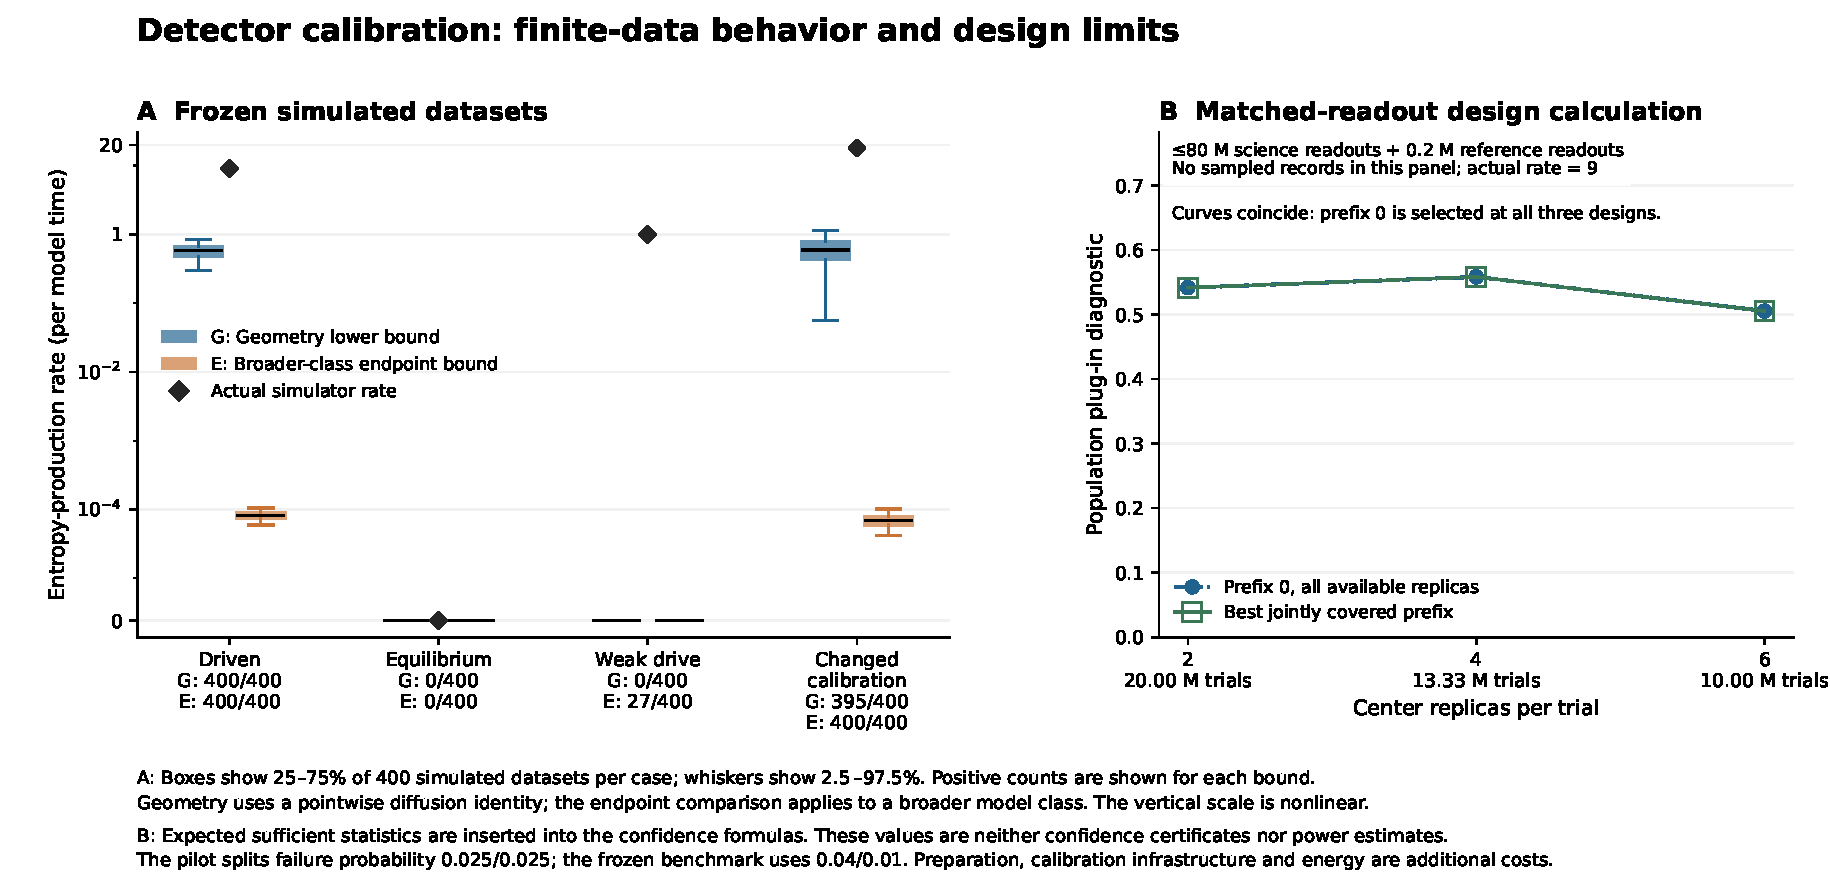
\includegraphics[width=\linewidth]{figures/detector_calibration.pdf}
\caption{Left: distributions over the $400$ simulated datasets in each case,
with boxes at the interquartile range and whiskers at empirical $2.5$th and
$97.5$th percentiles; the vertical axis uses a symmetric logarithmic scale.
Black diamonds mark the simulator entropy.
The endpoint bound has broader structural validity than the geometry bound.
Right: the separate prospective population diagnostic at matched target
readout ceilings, with the additional reference readings counted.  This
panel contains no random experimental outcomes or confidence certificates.}
\label{fig:dc-benchmark}
\end{figure}

\section{Acquisition costs and reproducibility}

Each dataset uses $79{,}999{,}998$ target readings, $200{,}000$ reference
readings and $80{,}199{,}998$ readings in total.  It requires
$13{,}333{,}333$ independent stationary preparations and $200{,}000$ controlled
reference preparations.  Four center shots share one physical exposure;
they still count as four detector readings.  There are $39{,}999{,}999$
target windows and $200{,}000$ reference windows.

The summed modeled target evolution duration is $n(2h+\tau)$:
$933{,}466.64333$ model-time units for the first three cases and
$933{,}533.309995$ for changed calibration.  The summed target exposure
durations are respectively $399.99999$ and $599.999985$; reference exposure
durations add $2$ and $3$.  These are sums over independent acquisitions,
not wall-clock durations or measured energy.  Stationary preparation, reset,
replica construction, clock calibration and shutter-control costs remain
unmeasured.  Fast categorical simulation does not make those physical
preparations inexpensive.

The authoritative files in \texttt{experiment/} are \texttt{contract.json},
\texttt{benchmark.json}, the compressed sufficient counts
\texttt{benchmark\_counts.json.gz}, and the first-generation
clock record \texttt{benchmark\_run.json}.  The contract binds
simulator, certifier and benchmark source hashes.  It was frozen on
2026-10-13 at 01:45:27 UTC; generation started at 01:45:40 and completed at
01:48:01 with four workers.  The choices preceding this freeze are retained
as prospective population diagnostics, not concealed as a preselected
universal design.  No stochastic pilot target records were used.

The seed rule is
$1032026400000+100000\,i+10\,r+s$ for case index $i$, repetition $r$ and
stream $s\in\{0,1,2\}$ for target, gain and step records.  Exact counts,
law enclosures, source bindings and the independent replay provide the
reproduction chain.  The stochastic-drive family proved in the preceding
chapter was not simulated in this bank.  Its analytic result and this
constant-drift detector benchmark remain distinct evidence.

\chapter{Completing access to stationary channel currents}
\label{ch:graph-access}

Conservation turns some inaccessible currents into measurable combinations of
other currents. It also has a definite limit: conservation of the aggregate
flow cannot determine how distinct physical channels divide that flow. This
chapter separates those two situations and gives exact sensor designs and
independently checkable uncertainty certificates.

The graph, its physical channels, and their assignment to pairs of states are
assumed known. The results do not reconstruct unknown hidden topology. They
specialize established linear observability, max-flow/min-cut, and spanning-tree
methods to a declared current-measurement contract. Conservation-based sensor
placement and measured cotrees have substantial prior literature, including
Bagajewicz and S\'anchez (2000) and He (2013); no priority claim is made for these
graph primitives. The purpose is to connect them explicitly to channel access,
sharp error guarantees, and physical realizability.

\section{The observation contract}

Let $G=(V,E)$ be a finite undirected multigraph without self-loops. Each physical
channel $e$ has an arbitrary reference orientation $u_e\to v_e$. Parallel edges
represent different transition mechanisms between the same pair of states.
The incidence matrix $B\in\mathbb R^{V\times E}$ has $-1$ at a channel's tail
and $+1$ at its head. A stationary current vector belongs to
\begin{equation}
 \mathcal J=\ker B.
 \label{eq:graph-current-class}
\end{equation}
Reference orientation is bookkeeping: every component of $j\in\mathcal J$
may be positive, negative, or zero. Initially, the model class imposes no
activity, rate, affinity, or current ceiling. Such additional restrictions can
change the sharp uncertainty bounds below.
The minimum-cut formulas require an incidence matrix. A general chemical
stoichiometric balance matrix need not have that form; it requires the more
general linear-identification and robust-recovery formulation rather than an
automatic application of these graph formulas.

A sensor for channel $s$ supplies either its exact native current $j_s$ or a
number $z_s$ with a justified bound $|z_s-j_s|\leq\epsilon_s$. The apparatus
need not observe the full state trajectory. This distinction matters: complete
state-resolved jump trajectories already identify aggregate transition rates
and their aggregate currents, subject to statistical uncertainty. The problem
here concerns sparse current access, including local intervention sensors that
report selected physical-channel currents.

Every impossibility or minimax statement is relative to the retained sensor
records. Richer raw observations may contain additional information. A sensor's
construction, calibration, and resource accounting must be supplied separately;
assigning an edge a cost does not by itself give that cost an energy meaning.

For a vertex set $U$, write
\begin{equation}
 \sigma_U(e)=\mathbf 1\{u_e\in U\}-\mathbf 1\{v_e\in U\}.
\end{equation}
Summing $Bj=0$ over the vertices of $U$ gives
\begin{equation}
 \sum_{e\in E}\sigma_U(e)j_e=0.
 \label{eq:graph-cut-conservation}
\end{equation}
Fix a target $e_0:u\to v$. For $u\in U$ and $v\notin U$, let
$C(U)=\{e\ne e_0:\sigma_U(e)\ne0\}$. This is the corresponding $u$--$v$
cut in $G\setminus\{e_0\}$.

\section{Exact identification and the minimum additional access}

\begin{theorem}[A target current requires a measured separating cut]
\label{thm:graph-target-identification}
Let $S\subseteq E\setminus\{e_0\}$ be the channels observed exactly. The
following conditions are equivalent:
\begin{enumerate}
 \item $j_S=j'_S$ implies $j_{e_0}=j'_{e_0}$ for every $j,j'\in\mathcal J$.
 \item $e_0$ is a bridge in $G\setminus S$.
 \item $S$ separates $u$ from $v$ in $G\setminus\{e_0\}$.
 \item Some $U$ containing $u$ and excluding $v$ satisfies $C(U)\subseteq S$.
\end{enumerate}
Whenever these conditions hold,
\begin{equation}
 j_{e_0}=-\sum_{s\in C(U)}\sigma_U(s)j_s.
 \label{eq:graph-target-estimator}
\end{equation}
\end{theorem}

\begin{proof}
Suppose a path from $v$ to $u$ remains after deleting $S$ and $e_0$. Send one
unit of signed flow along that path, and one unit along $e_0$ from $u$ to $v$.
The resulting vector $h$ obeys $Bh=0$, $h_S=0$, and $h_{e_0}=1$. Thus $j=0$
and $j'=h$ have identical sensor records and different target currents.
Identification is impossible.

If no such path remains, let $U$ be the component of $u$ after those deletions.
Then $v\notin U$, and every original crossing edge except $e_0$ belongs to
$S$. Equation~\eqref{eq:graph-cut-conservation}, with $\sigma_U(e_0)=1$,
gives~\eqref{eq:graph-target-estimator}. It determines the target from the
record. The existence of the alternative path is exactly the failure of $e_0$
to be a bridge in $G\setminus S$, proving all equivalences.
\end{proof}

An original bridge has stationary current zero. The theorem then requires no
sensor: conservation already fixes its current. Parallel channels must not be
collapsed before applying the theorem. A second unsensed channel between $u$
and $v$ supplies an alternative path of length one and hence an ambiguity.

\begin{corollary}[Minimum additional sensing cost]
\label{cor:graph-minimum-cost}
Give each eligible nontarget channel a nonnegative acquisition cost $c_s$.
Other channels cannot be selected. The minimum total cost of an exact indirect
target measurement is
\begin{equation}
 \min_{U:\,u\in U,\,v\notin U}\ \sum_{s\in C(U)}c_s,
 \label{eq:graph-installation-cut}
\end{equation}
where a cut containing an ineligible channel has infinite cost. If direct
measurement of $e_0$ is also allowed, take the smaller of its cost and the
indirect optimum.
\end{corollary}

\begin{proof}
Every successful sensor set contains $C(U)$ for some admissible $U$, by
Theorem~\ref{thm:graph-target-identification}. Nonnegative costs make its
total cost at least that of this cut. Conversely, measuring exactly the edges
of a minimum cut supplies the estimator~\eqref{eq:graph-target-estimator}.
\end{proof}

This is an ordinary minimum-cut computation with a scientific interpretation.
Its optimality is for the supplied sensor menu and additive cost model. It
does not assert that the menu contains every physically possible experiment.

\section{A sharp error bound, including nonlinear estimators}

Let $S$ now supply noisy current estimates
\begin{equation}
 z_s=j_s+\eta_s,\qquad |\eta_s|\leq\epsilon_s,\qquad s\in S.
 \label{eq:graph-box-record}
\end{equation}
The full Cartesian error box is allowed. This is an adversarial uncertainty
set, not an assumption of probabilistic independence. Define the deterministic
minimax radius
\begin{equation}
 R_S=\inf_f\ \sup_{\substack{j\in\ker B\\|\eta_s|\leq\epsilon_s}}
       \left|f(j_S+\eta)-j_{e_0}\right|,
 \label{eq:graph-minimax-definition}
\end{equation}
where $f$ ranges over all estimators, including nonlinear ones.

\begin{theorem}[The exact radius is an error-weighted cut]
\label{thm:graph-exact-radius}
Under~\eqref{eq:graph-current-class} and~\eqref{eq:graph-box-record},
\begin{equation}
 R_S=\min_{\substack{U:\,u\in U,\,v\notin U\\C(U)\subseteq S}}
                 \sum_{s\in C(U)}\epsilon_s.
 \label{eq:graph-exact-radius}
\end{equation}
The value is $+\infty$ when there is no admissible cut. For a finite minimum,
the signed cut-sum estimator attains the radius globally.
\end{theorem}

\begin{proof}
For any admissible cut, use
$f(z)=-\sum_{s\in C(U)}\sigma_U(s)z_s$. Subtracting the exact conservation
identity shows that its error is a signed sum of the $\eta_s$. Its absolute
value is at most $\sum_{s\in C(U)}\epsilon_s$. Minimizing over cuts gives the
upper bound.

For the matching lower bound, remove $e_0$. Give each sensor edge capacity
$\epsilon_s$ in either direction, and every unobserved edge infinite
capacity. If a finite separating cut exists, undirected max-flow/min-cut gives
a signed flow of value $R$ from $v$ to $u$, where $R$ is the right side
of~\eqref{eq:graph-exact-radius}. Close the flow with current $R$ on $e_0$.
The resulting circulation $h$ satisfies
\begin{equation}
 Bh=0,\qquad h_{e_0}=R,\qquad |h_s|\leq\epsilon_s\quad(s\in S).
 \label{eq:graph-dual-witness}
\end{equation}
Both $j=h$ with errors $\eta=-h_S$ and $j=-h$ with errors $\eta=h_S$ produce
the identical record $z=0$. Their target values are $R$ and $-R$. Any single
estimate $f(0)$ has error at least $R$ in one of the two cases. This lower
bound applies to every estimator and matches the upper bound.

For completeness, the infinite-capacity construction can be made finite. If
there is no entirely unobserved $v$--$u$ path, assign every unobserved edge a
capacity strictly larger than $\sum_{s\in S}\epsilon_s$. At least one cut
uses only sensor edges, so a minimum cut never crosses an unobserved edge.
The finite-capacity max-flow theorem therefore gives exactly the required
flow. If an entirely unobserved path does exist, the unit circulation in the
proof of Theorem~\ref{thm:graph-target-identification} can be scaled without
bound while leaving every sensor record unchanged. Then $R_S=+\infty$.
\end{proof}

The theorem explains why averaging redundant sensors need not improve a
worst-case box guarantee. It does not prohibit statistical improvement under a
specified noise law or an uncertainty set that excludes the least-favorable
error combinations. Known rate or activity bounds can also reduce the sharp
radius by restricting the allowed currents.

\paragraph{A certificate requiring no optimization.}
A finite certificate consists of a vertex cut $U$ and a circulation $h$. A
checker verifies $C(U)\subseteq S$, the identities and bounds
in~\eqref{eq:graph-dual-witness}, and
$h_{e_0}=\sum_{s\in C(U)}\epsilon_s$. These checks establish matching lower
and upper bounds without trusting or rerunning the search algorithm. An
infinite certificate instead supplies $Bh=0$, $h_{e_0}=1$, and $h_S=0$.

\section{Aggregate access and the internal channel obstruction}

Partition the physical channels into bundles $\mathcal B$, one for each
unordered pair of endpoint states. Choose one canonical orientation per bundle.
Let $A$ take signed bundle sums, so $k=Aj$ is the vector of aggregate currents
and
\begin{equation}
 B=\bar B A,
 \label{eq:graph-bundle-factorization}
\end{equation}
where $\bar B$ is the incidence matrix of the underlying simple graph.
Suppose bundle totals are known exactly for $T\subseteq\mathcal B$, and
individual channels are sensed exactly for $S\subseteq E$. These aggregate
readings are treated as already available. If their calibration errors are
nonzero, a robust linear-observation formulation is needed instead of silently
using the exact identities below.

Write $r_b=|b\setminus S|$ for the number of unsensed channels in bundle $b$.
Form a graph $H$ on all vertices $V$, including isolated vertices, with one
edge for each bundle $b\notin T$ having $r_b>0$. Let $c(H)$ denote its number
of connected components.

\begin{theorem}[Two distinct sources of current ambiguity]
\label{thm:graph-mixed-access}
The homogeneous ambiguity space
\begin{equation}
 \mathcal N=\{h:Bh=0,\ A_T h=0,\ h_S=0\}
\end{equation}
has dimension
\begin{equation}
 \dim\mathcal N
 =\sum_{b\in\mathcal B}\max(r_b-1,0)
       +|E(H)|-|V|+c(H).
 \label{eq:graph-mixed-dimension}
\end{equation}
An unsensed target $e_0$ in bundle $b_0$ is identifiable if and only if
\begin{equation}
 r_{b_0}=1
 \quad\hbox{and}\quad
 \bigl(b_0\in T\ \hbox{or $b_0$ is a bridge of $H$}\bigr).
 \label{eq:graph-mixed-target}
\end{equation}
\end{theorem}

\begin{proof}
After imposing $h_S=0$, each nonempty unsensed bundle has $r_b$ free channel
coordinates. Taking its signed sum maps these coordinates onto one aggregate
coordinate. The kernel of that map has dimension $r_b-1$. Because bundles have
disjoint channel coordinates, their internal kernels form a direct sum of
dimension $\sum_b\max(r_b-1,0)$.

Known aggregate variations vanish. All remaining aggregate variations must
satisfy conservation on $H$, by~\eqref{eq:graph-bundle-factorization}; hence
they belong to $\ker B_H$. Conversely, choose one unsensed representative
channel in each nonempty bundle. Any circulation on $H$ can be lifted by
assigning its aggregate current, with the appropriate orientation sign, to
that representative and assigning zero to every other channel. Known bundle
variations remain zero, and $Bh=\bar BAh=0$. The map from $\mathcal N$ onto
$\ker B_H$ is therefore surjective, with exactly the internal kernel described
above. The dimension formula follows from
$\dim\ker B_H=|E(H)|-|V|+c(H)$.

If $r_{b_0}\geq2$, one can change the target and compensate on another
unsensed channel in the same bundle. Choose the signs so that their aggregate
variation is zero. This changes $h_{e_0}$ while preserving all supplied
measurements and conservation, so the target is unidentifiable. If
$r_{b_0}=1$, the target variation equals the aggregate variation of $b_0$ up
to orientation. It vanishes when $b_0\in T$. Otherwise, it vanishes for every
circulation on $H$ precisely when $b_0$ is a bridge, by
Theorem~\ref{thm:graph-target-identification}. This proves both directions
of~\eqref{eq:graph-mixed-target}.
\end{proof}

The first term in~\eqref{eq:graph-mixed-dimension} is ambiguity between
physical channels sharing the same endpoints. The second is circulation
ambiguity among unknown aggregate edges. The decomposition need not select a
preferred representative channel, but its dimension and target criterion are
independent of that choice.

In particular, if every aggregate current is known, then $\ker A\subseteq\ker
B$ by~\eqref{eq:graph-bundle-factorization}. Conservation supplies no further
constraint on the internal split. It cannot distinguish two physical channels
whose currents change oppositely while leaving the aggregate unchanged. This
is a necessary-access obstruction: some measurement or intervention must
distinguish those channels, unless additional physical assumptions already
fix their relation.

\section{Constructive completion with mixed access}

\begin{proposition}[Minimum indirect access for one target]
\label{prop:graph-mixed-completion}
Assume all nontarget channels can be sensed at nonnegative costs $c_e$, and
the exact aggregate readings in $T$ are already available. A minimum-cost
indirect sensor set for target $e_0\in b_0$ is obtained as follows:
\begin{enumerate}
 \item Sense every other channel in $b_0$.
 \item If $b_0\in T$, stop.
 \item Otherwise, build the simple graph of bundles not in $T$, remove
       $b_0$, and give each other bundle the cost
       $C_b=\sum_{e\in b}c_e$.
 \item Find a minimum cut between the endpoints of $b_0$ and sense every
       physical channel in every bundle crossing that cut.
\end{enumerate}
\end{proposition}

\begin{proof}
Every other channel in $b_0$ must be sensed: otherwise the internal two-channel
ambiguity in Theorem~\ref{thm:graph-mixed-access} survives. These costs are
unavoidable. If the target aggregate is known, the forced sensors already
determine the target by subtraction.

If the target aggregate is unknown, it must become a bridge of the residual
unknown-bundle graph. A nontarget bundle disappears from that graph exactly
when all its physical channels are sensed, at cost $C_b$. Partially sensing a
bundle leaves at least one channel able to carry its arbitrary aggregate
variation. By Theorem~\ref{thm:graph-target-identification}, every successful
design must therefore remove the bundles of a separating cut. Its additional
cost is at least the minimum cut cost. Sensing all channels on that minimum cut
makes the target a bridge and attains the bound. These bundles are disjoint
from $b_0$, so their costs add to the forced parallel-channel costs.
\end{proof}

\begin{proposition}[Minimum access for every physical-channel current]
\label{prop:graph-all-targets}
Suppose every channel has a nonnegative sensing cost. Define
$w_b=\max_{e\in b}c_e$. The minimum total cost for recovering every current,
given exact aggregate access on $T$, is
\begin{equation}
 \sum_{e\in E}c_e
 -\sum_{b\in T}w_b
 -\max_{F\text{ forest in }\mathcal B\setminus T}\ \sum_{b\in F}w_b.
 \label{eq:graph-all-target-optimum}
\end{equation}
A maximum-weight spanning forest of the unknown-bundle graph supplies an
optimal design.
\end{proposition}

\begin{proof}
Full recovery requires zero ambiguity dimension in
Theorem~\ref{thm:graph-mixed-access}. Thus at most one channel may remain
unsensed in each bundle, and the unknown bundles retaining such a channel must
form a forest. Conversely, these two conditions make both terms of the
dimension formula zero and hence suffice.

To maximize saved sensing cost, retain a maximum-cost unsensed channel in
each known-total bundle; these choices impose no cycle constraint. For an
unknown-total bundle that is retained, the best saved cost is also $w_b$.
The set of retained unknown bundles must be a forest, so a maximum-weight
forest maximizes their total savings. Subtracting both savings from the cost
of sensing all channels gives~\eqref{eq:graph-all-target-optimum}. Nonnegative
weights allow a maximizing forest to be extended to a spanning forest in
each component without decreasing its weight.
\end{proof}

With no aggregate access, this reduces to the familiar measured-cotree rule
on the physical multigraph. With every aggregate known, one maximum-cost
channel per bundle can be left unsensed, but all other channel splits require
individual information. The algorithms are exact for their declared access
and price assumptions; uncertain aggregate measurements or unavailable
channels require the corresponding constraints to be retained explicitly.

\section{The ambiguity witnesses are realizable by positive rates}

Allowing signed currents does not require negative transition rates.

\begin{proposition}[Realization at a prescribed stationary distribution]
\label{prop:graph-physical-realization}
Let $j\in\ker B$ be finite, and let $\pi$ be any strictly positive probability
distribution on $V$. Choose $t_e>|j_e|/2$ for every channel and define
\begin{equation}
 q_e(u_e,v_e)=\frac{t_e+j_e/2}{\pi_{u_e}},\qquad
 q_e(v_e,u_e)=\frac{t_e-j_e/2}{\pi_{v_e}}.
 \label{eq:graph-rate-realization}
\end{equation}
The resulting bidirectional channel rates are strictly positive. Their sum
defines a continuous-time Markov chain with stationary distribution $\pi$ and
channel currents exactly $j$. If the support graph is connected, the chain is
irreducible.
\end{proposition}

\begin{proof}
The strict traffic inequality makes both numerators positive. The stationary
forward and reverse channel fluxes are respectively $t_e+j_e/2$ and
$t_e-j_e/2$, whose difference is $j_e$. Summing their net contributions at
each vertex gives $Bj=0$, so incoming and outgoing stationary fluxes balance.
Setting generator diagonals to minus outgoing rates therefore gives
$\pi Q=0$. Connected bidirectional support makes every state reachable from
every other state and hence makes the chain irreducible.
\end{proof}

A finite pair of least-favorable currents $h$ and $-h$ can use the same $\pi$
and the same traffic $t_e>|h_e|/2$. Thus the sharp-error witnesses can have
identical stationary occupations and positive finite rates. An unbounded
impossibility result uses arbitrarily large finite rates across the model
class, not an infinite rate in an individual model. A fixed physical device
may impose traffic, fuel, or affinity limits that restrict this class. Fixed
chemical stoichiometry and fixed reservoirs also introduce constraints not
encoded by conservation alone.

\section{Worked example and reproducible interface}

Consider states $A,B,C,D$ and six physical channels:
\begin{equation}
 e_0:A\to B,\quad p:A\to B,\quad
 a:A\to C,\quad b:B\to C,\quad c:C\to D,\quad d:D\to A.
\end{equation}
Suppose only $p,a,d$ are measured, with respective error radii
$1/100$, $1/50$, and $3/100$. The cut $U=\{A\}$ gives
\begin{equation}
 \widehat j_{e_0}=-z_p-z_a+z_d,\qquad R=\frac{3}{50}.
\end{equation}
The following matching circulation certifies sharpness:
\begin{equation}
 (h_{e_0},h_p,h_a,h_b,h_c,h_d)
 =\left(\frac3{50},-\frac1{100},-\frac1{50},
                  \frac1{20},\frac3{100},\frac3{100}\right).
\end{equation}
It obeys conservation, reaches the target error radius, and respects all
sensor error bounds. Its two signs can be realized by
\eqref{eq:graph-rate-realization} with common stationary occupations.

If all five bundle totals are instead known exactly, one ambiguity remains:
the split between $e_0$ and $p$. Reading $p$ resolves it. Conservation alone
cannot. For a separate exact sensing-cost example, assign costs
$c_p=2,c_a=3,c_b=4,c_c=5,c_d=6$. The minimum indirect design for $e_0$ measures
$p$ and $b$, at total cost $6$. Conservation gives $j_{e_0}=-j_p+j_b$.
This acquisition-price example and the preceding error-radius example use
different declared inputs; their numbers must not be interpreted as the same
resource quantity.

The implementation is in \texttt{code/graph\_access.py}. It accepts exact
integers, rational strings, or \texttt{Fraction} values and rejects floating
point capacities. Its main interfaces are:
\begin{description}
 \item[\texttt{target\_cut}] Finds a minimum cut for supplied acquisition
 costs or sensor-error capacities, returning a cut and matching circulation.
 \item[\texttt{verify\_target\_cut}] Checks the certificate directly,
 without invoking an optimization algorithm.
 \item[\texttt{mixed\_observability}] Returns the internal-channel and
 network-cycle ambiguity dimensions and all identifiable target channels.
 \item[\texttt{target\_completion}] Returns a minimum indirect sensor set
 with exact aggregate access; direct measurement of the target is excluded.
 \item[\texttt{all\_target\_completion}] Returns an optimal full-current
 design using the maximum-weight forest construction.
 \item[\texttt{realize\_currents}] Constructs positive rational channel
 rates at a prescribed strictly positive stationary distribution.
\end{description}
The rational example certificates and rate realization are saved in
\texttt{results/graph\_access.json}. Reproduction commands are
\begin{verbatim}
python code/graph_access.py
python -m unittest discover -s tests -p test_graph_access.py -v
\end{verbatim}

Author tests compare cut values with exhaustive vertex partitions, mixed
observability with an independent rational rank calculation, and both sensor
designs with exhaustive subsets. Separate internal review additionally checked
2,197 mixed-observation configurations, 65 completion instances, and 160 cut
cases. These checks support the implementation; the proofs establish the
general results. External peer review and experimental validation remain
separate requirements.

\chapter{Precision, calibration, and acquisition energy}
\label{ch:access-resources}

An intervention can make a current identifiable while leaving its numerical
value too uncertain to be useful. Conversely, a very precise instrument can
remain blind to the desired distinction. Experimental design must address both
questions: which observations determine the target, and which attainable error
bounds make the answer useful?

This chapter connects those questions for conserved currents. It first treats
shared calibration errors, then optimizes a declared relation between sensor
precision and acquisition energy. A sharp change occurs when irreducible
calibration errors are admitted: a design problem solvable by one minimum cut
becomes NP-complete in general. We nevertheless obtain inexpensive certificates
that bound the optimum and sometimes determine it exactly.

The ingredients---linear-programming duality, max-flow/min-cut, H\"older's
inequality, and supporting hyperplanes---are established mathematics. Their
role here is to provide a connected, checkable experimental-design method.
The energy results are conditional on an explicit sensor contract. They are
not universal thermodynamic lower bounds.

\section{Recovering a target in the presence of shared nuisance}

Let $j\in\mathbb R^m$ denote a vector of currents and let $Bj=0$ encode known
conservation laws. For a graph incidence matrix, a column has $-1$ at the tail
and $+1$ at the head of its oriented edge. Negative currents are permitted;
the orientation only fixes the sign convention. Suppose the available
observations satisfy
\begin{equation}
 y=Hj+A\eta+e,\qquad |e_i|\leq\varepsilon_i,
 \label{eq:res-observation}
\end{equation}
where $\eta\in\mathbb R^k$ is an unknown fixed calibration nuisance. Its effect
across observations is the known matrix $A$. The scientific target is $b^Tj$.

Throughout this section, the admissible parameter space is the entire linear
space $\ker B$, the nuisance is unrestricted, and the error set is the full
coordinatewise box. These assumptions define the minimax claim. Bounded
traffic, known affinities, correlated errors, or prior parameter bounds can
change the sharp answer.

\begin{theorem}[Constrained linear minimax recovery]
\label{thm:res-nuisance}
Under \eqref{eq:res-observation}, the minimum, over all estimators, of the
worst-case absolute error is
\begin{align}
 R
 &=\min_{w,\phi}\ \sum_i\varepsilon_i|w_i|
 &&\text{subject to }H^Tw+B^T\phi=b,\quad A^Tw=0,
 \label{eq:res-primal}\\
 &=\max_{h,z}\ b^Th
 &&\text{subject to }Bh=0,\quad |Hh+Az|\leq\varepsilon.
 \label{eq:res-dual}
\end{align}
If the constraints in \eqref{eq:res-primal} have no solution, $R=+\infty$.
Otherwise the finite optima are attained, and an optimal estimator is $w^Ty$.
\end{theorem}

\begin{proof}
The identities in \eqref{eq:res-primal} give
$w^Ty-b^Tj=w^Te$, whose absolute value is at most
$\sum_i\varepsilon_i|w_i|$. For any feasible $(h,z)$ in
\eqref{eq:res-dual}, the two parameter pairs $(j,\eta)=(h,z)$ and $(-h,-z)$
produce the same observation $y=0$ when their errors are respectively
$-(Hh+Az)$ and $Hh+Az$. Their targets are $b^Th$ and $-b^Th$, so every
estimator incurs maximum error at least $|b^Th|$. Linear-programming duality
equates the two bounds. Equivalently, append the exact observations $Bj=0$
to \eqref{eq:res-observation} and apply linear optimal recovery to $(j,\eta)$.
If the primal identities are infeasible, the annihilator alternative provides
$Bh=0$, $Hh+Az=0$, and $b^Th\ne0$. Scaling this direction proves unbounded
ambiguity. Finite-dimensional linear programs attain their finite optima,
including the cases of redundant constraints and zero error radii.
\end{proof}

The certificate contains the estimator weights $(w,\phi)$ and the
least-favorable perturbation $(h,z)$. Checking linear identities, error bounds,
and equality of the two objective values establishes optimality without
rerunning the optimizer. The small exact solver supplied with this release
enumerates supports and vertices; that implementation is intended for examples,
not large-scale general linear programming.

\paragraph{A shared bias can be cancelled; an arbitrary bias cannot.}
On an oriented triangle, conservation gives $j_1=j_2=j_3=J$. Consider
\[
 y_1=J+\eta+e_1,\qquad y_2=-J+\eta+e_2.
\]
The estimator $(y_1-y_2)/2$ has exact worst-case error
$(\varepsilon_1+\varepsilon_2)/2$. For radii $1/10$ and $1/5$, the result is
$3/20$. If both responses are $J+\eta$, the current remains unidentifiable.
It also remains unidentifiable if the two offsets are independently unknown.
The useful operation is a physical response change that reverses the current
contribution while preserving the shared offset. Negating an existing recorded
number reverses both contributions and creates no additional access.

\paragraph{The lower-bound currents can have positive physical rates.}
For a connected bidirectional network, fix any positive stationary distribution
$\pi$. Given a finite circulation $j$, choose symmetric edge traffics
$t_e>|j_e|/2$. On an edge $e:u\to v$, set
\[
 q^e_{uv}=\frac{t_e+j_e/2}{\pi_u},\qquad
 q^e_{vu}=\frac{t_e-j_e/2}{\pi_v}.
\]
All rates are positive, $\pi$ is stationary by conservation, and the channel
current is $j_e$. A least-favorable pair $\pm h$ can use the same $\pi$ and
the same traffics $t_e>|h_e|/2$. Thus the circulation lower bound does not rely
on negative transition rates. This construction does not imply that every
fixed device with bounded rates can realize the entire current space.

\section{The exact uncertainty of one hidden current}

Let $e_0:u\to v$ be an edge whose current cannot be measured directly. Remove
that edge from the graph. Some remaining edges have sensor records
$y_e=j_e+e_e$, with $|e_e|\leq\varepsilon_e$; other edges are unobserved.
The errors jointly range over the full box. No probabilistic independence
assumption is involved.

\begin{proposition}[Current uncertainty as a minimum cut]
\label{prop:res-current-cut}
Over the full circulation space, the exact minimax absolute error for $j_{e_0}$
is the minimum $u$--$v$ cut capacity in the graph without $e_0$, assigning
capacity $\varepsilon_e$ to a measured edge and infinite capacity to an
unobserved edge. An unobserved $u$--$v$ path makes the error unbounded. If
$e_0$ is a bridge, its stationary current is zero and needs no measurement.
\end{proposition}

\begin{proof}
Conservation expresses the target current as a signed sum of the other currents
crossing any separating cut. A cut containing only measured edges therefore
gives an estimator with error at most the sum of its radii. A maximum flow from
$v$ to $u$ through the remaining graph, closed by a flow through $e_0$, gives a
circulation $h$ with $|h_e|\leq\varepsilon_e$ on every measured edge. The pair
$\pm h$ has a common possible record and target separation $2h_{e_0}$.
Max-flow/min-cut equates these bounds. An entirely unobserved return path
supports an arbitrarily scaled invisible circulation. A bridge cannot carry
a nonzero conserved current.
\end{proof}

The same minimum-cut algorithm can optimize installation cost, error, or a
transformed parameter for acquisition energy. These are different inputs and
different scientific claims. An error capacity must not be interpreted as an
energy cost merely because the same graph algorithm processes it.

\section{A declared relation between precision and acquisition energy}

Assume that an available sensor has the calibrated error contract
\begin{equation}
 \varepsilon_e(E_e)
 =\delta_e+\sqrt{\frac{a_e}{E_e}}
 =\delta_e+\sqrt{\frac{q_e^3}{E_e}},
 \qquad q_e=a_e^{1/3}>0,\quad \delta_e\geq0,
 \label{eq:res-energy-law}
\end{equation}
where $E_e>0$ is acquisition energy in consistently declared units. The floor
$\delta_e$ represents an error that additional acquisition energy cannot
remove under this contract. Zero allocation means no reading and hence
unbounded uncertainty.

Equation \eqref{eq:res-energy-law} is an input to the design problem. It must
be justified for the estimated \emph{current}, including the response model
that converts a detector output into that current. A square-root uncertainty
law for raw photon or transition counts does not by itself establish the same
law after an uncertain dynamical inversion. Finite pulses, poorly known gains,
and systematic response errors can produce different exponents or additional
floors.

The optimization below concerns fixed sensor selections and nonadaptive,
continuous energy allocations. Integer record counts, power limits, minimum
pulse durations, and history-dependent acquisition require additional
constraints. Preparation, control, reset, calibration, installation, and
thermal-support energy are additional unless explicitly included in $E_e$.

If \eqref{eq:res-energy-law} describes a simultaneous confidence envelope
valid with probability at least $1-\alpha$, the resulting target-error bound
has that same confidence. Marginal guarantees for individual sensors do not
automatically give a joint guarantee. If the envelope is conservative, the
optimum below is the optimum certified by the declared adversarial box; it
need not be the minimum energy of every physically conceivable experiment.

\begin{theorem}[Optimal allocation on a cut]
\label{thm:res-cut-allocation}
For a nonempty sensor cut $C$, define
\[
 Q_C=\sum_{e\in C}q_e,\qquad
 \Delta_C=\sum_{e\in C}\delta_e.
\]
The minimum acquisition energy giving target-current error at most $\tau>0$
through that cut is
\begin{equation}
 E_C^*=\frac{Q_C^3}{(\tau-\Delta_C)^2},\qquad \tau>\Delta_C.
 \label{eq:res-cut-energy}
\end{equation}
It is attained by
\begin{equation}
 E_e=\frac{Q_C^2q_e}{(\tau-\Delta_C)^2},\qquad
 \varepsilon_e=\delta_e+
       \frac{(\tau-\Delta_C)q_e}{Q_C}.
 \label{eq:res-allocation}
\end{equation}
No finite energy suffices if $\tau\leq\Delta_C$. An empty cut has zero cost.
\end{theorem}

\begin{proof}
Put $x_e=\sqrt{q_e^3/E_e}>0$. Feasibility requires
$\sum_{e\in C}x_e\leq\tau-\Delta_C$. H\"older's inequality gives
\[
 Q_C=\sum_{e\in C}
       \left(\frac{q_e^3}{x_e^2}\right)^{1/3}x_e^{2/3}
 \leq\left(\sum_{e\in C}E_e\right)^{1/3}
       \left(\sum_{e\in C}x_e\right)^{2/3}.
\]
This proves the lower bound in \eqref{eq:res-cut-energy}, and
\eqref{eq:res-allocation} attains equality.
\end{proof}

\begin{corollary}[Global sensor and energy design]
\label{cor:res-global-energy}
Under the full circulation and box-error model, the optimum over fixed
allocations, arbitrary sensor subsets, and all estimators is
\begin{equation}
 E^*=\min_C\frac{Q_C^3}{(\tau-\Delta_C)^2},
 \label{eq:res-global-energy}
\end{equation}
where the minimum ranges over sensor-only separating cuts with
$\Delta_C<\tau$, with the bridge exception assigned zero energy.
\end{corollary}

\begin{proof}
Every successful allocation has some separating cut whose summed error is
at most $\tau$, by Proposition~\ref{prop:res-current-cut}. Its total acquisition
energy is at least the optimal allocation on that cut. Conversely, a cut
estimator with \eqref{eq:res-allocation} attains the displayed value.
\end{proof}

The formula also supplies a finite-energy feasibility test. Let $\rho$ be the
minimum cut sum of $\delta_e$, with unavailable sensors assigned infinite
capacity. For a nonbridge target with strictly positive $a_e$, finite energy
is possible exactly when $\tau>\rho$. At $\tau=\rho$, more acquisition can
approach the floor but cannot attain it at finite energy.

\begin{remark}[Other calibrated precision exponents]
The allocation argument is not specific to a square-root law. For a declared
contract $\varepsilon_e=\delta_e+(a_e/E_e)^{1/p}$ with $p>0$, put
$q_e=a_e^{1/(p+1)}$. The same H\"older argument gives
$E_C^*=Q_C^{p+1}/(\tau-\Delta_C)^p$ and
$E_e=Q_C^p q_e/(\tau-\Delta_C)^p$.
This algebraic extension does not establish which exponent a physical sensor
obeys. The exact allocation software in this release implements $p=2$.
\end{remark}

\section{An efficient exact case and a complexity boundary}

\subsection{Zero calibration floors}
If every $\delta_e=0$, minimizing \eqref{eq:res-global-energy} amounts to
minimizing $Q_C$. Thus one minimum cut with edge capacities $q_e$ gives
\begin{equation}
 E^*=\frac{\left(\min_C\sum_{e\in C}q_e\right)^3}{\tau^2}.
 \label{eq:res-ideal-energy}
\end{equation}
The cut chooses the sensors and \eqref{eq:res-allocation} chooses their
precision. A matching flow certifies that no alternative sensor set can have
less energy under the contract.

For rational $q_e$ and $\tau$, all quantities in this certificate are rational.
Equivalently, the input sensor family has $a_e=q_e^3$. General cube roots require
algebraic or certified interval arithmetic; the exact implementation does not
silently round them. The checker verifies the graph, capacity bounds,
conservation, cut--flow equality, and the allocation identities, against the
externally supplied sensor parameters.

\subsection{Irreducible calibration floors}
Consider the following decision problem. Given a graph, target edge, available
sensors with rational $q_e>0$ and $\delta_e\geq0$, rational accuracy $\tau>0$,
and rational acquisition budget $L\geq0$, does a fixed allocation achieve
worst-case target error at most $\tau$ with total energy at most $L$?

\begin{theorem}[Floor-aware design complexity]
\label{thm:res-floor-hardness}
For binary-encoded rational inputs, this decision problem is NP-complete.
NP-hardness holds even when all nontarget sensors are available, all calibration floors
are positive, every cut is feasible at finite energy, and the graph is a target
edge plus parallel two-edge paths with distinct internal vertices.
\end{theorem}

\begin{proof}
A separating cut is a polynomial-size witness. Compute its rational $Q_C$ and
$\Delta_C$ and check
\[
 \tau>\Delta_C,\qquad Q_C^3\leq L(\tau-\Delta_C)^2.
\]
The corresponding allocation has polynomial encoding length. An empty cut is
handled separately. Thus the decision problem is in NP.

For hardness, reduce PARTITION on positive integers $v_1,\ldots,v_n$ whose sum
is $V$. Set $\beta=V$. For each $i$, introduce the path $s$--$i$--$t$, with
sensor parameters
\[
 (q,\delta)=(\beta,\beta+v_i)
 \quad\text{on }s\text{--}i,\qquad
 (q,\delta)=(\beta+v_i,\beta)
 \quad\text{on }i\text{--}t.
\]
The target is the direct edge $s$--$t$. Every separating cut in the graph
without the target chooses one edge from each path. If $S$ indexes its
second-edge choices, then
\[
 Q=n\beta+\sum_{i\in S}v_i,\qquad
 \Delta=n\beta+V-\sum_{i\in S}v_i,
 \qquad Q+\Delta=K=2n\beta+V.
\]
Set
\[
 Q_*=n\beta+\frac V2,\qquad
 \tau=K-\frac{Q_*}{3},\qquad
 L=\frac{9Q_*}{4}.
\]
All numbers have polynomial bit length. Every cut has
$\tau-\Delta=Q-Q_*/3>0$, because $Q\geq nV>Q_*/3$. Its energy is
\[
 f(Q)=\frac{Q^3}{(Q-Q_*/3)^2}.
\]
The exact factorization
\[
 4x^3-9Q_*(x-Q_*/3)^2=(x-Q_*)^2(4x-Q_*)
\]
shows that $f(x)\geq9Q_*/4$ for $x>Q_*/3$, with equality exactly at $x=Q_*$.
There is therefore a feasible cut with energy at most $L$ precisely when
$\sum_{i\in S}v_i=V/2$. This completes the reduction.
\end{proof}

The reduction establishes NP-hardness through PARTITION; it does not establish
strong NP-hardness or rule out useful approximation, pseudopolynomial methods,
or tractable subclasses. It separates an efficiently checkable design from
an efficient general search for the optimum. The result also does not mean
that scientific access is uncomputable.

Budgeted terminal-cut problems already have a substantial complexity literature.
For example, Aissi and Mahjoub's treatment of minimum $s$--$t$ cuts with budget
constraints discusses related hardness results and earlier work.\footnote{Primary
manuscript: \url{https://www.lamsade.dauphine.fr/~mahjoub/Papers/Paper-Aissi-Mahjoub-2023.pdf}.}
The direct reduction above addresses the particular nonlinear
precision--energy objective used here; it is not a claim to have discovered
the hardness of multiobjective cuts.

\section{Global certificates when exact design is difficult}

Computational hardness does not prevent a useful guarantee on a proposed
design. For any chosen rational support parameter $\lambda>0$, assign capacities
\begin{equation}
 c_e(\lambda)=3\lambda^2q_e+2\lambda^3\delta_e,
 \label{eq:res-support-capacity}
\end{equation}
and let $W(\lambda)$ be their minimum cut value.

\begin{proposition}[Supporting-cut energy bracket]
\label{prop:res-support}
The optimum floor-aware acquisition energy obeys
\begin{equation}
 E^*\geq\max\{0,W(\lambda)-2\tau\lambda^3\}.
 \label{eq:res-support-bound}
\end{equation}
If a minimum cut returned for \eqref{eq:res-support-capacity} satisfies
$\Delta_C<\tau$, its allocation in \eqref{eq:res-allocation} provides a feasible
upper bound. Matching bounds certify global optimality.
\end{proposition}

\begin{proof}
For a feasible cut, write $s=\tau-\Delta_C>0$ and $x=Q_C/s$. Then
\[
 \frac{Q_C^3}{s^2}
 -\left(3\lambda^2Q_C-2\lambda^3s\right)
 =s(x-\lambda)^2(x+2\lambda)\geq0.
\]
Minimizing the supporting expression $3\lambda^2Q_C-2\lambda^3s$ over all cuts gives
$W(\lambda)-2\tau\lambda^3$. Allowing infeasible cuts in that minimum can
only lower it, so it remains a valid lower bound. Energy is also nonnegative.
The upper bound follows from the explicit feasible allocation.
\end{proof}

One max-flow computation supplies the lower-bound certificate. Its flow and
cut can be checked without rerunning the optimization. Repeating this procedure
for a declared finite set of support parameters gives the maximum certified
lower bound and the minimum feasible upper bound encountered. This is a
supporting-hyperplane bound, not a general exact solution of the NP-complete
problem.

The hardness construction also supplies a useful failure control. At
$\lambda=3/2$, the weights of $q_e$ and $\delta_e$ coincide. The lower bound is
exactly the PARTITION threshold $L$ for every instance. If the integers have no
equal partition, the true optimum is strictly larger. Thus a valid global
lower bound need not be attainable by any physical sensor cut.

\section{A complete design example}

Consider three vertices $s,a,t$. Besides the inaccessible target $s$--$t$,
there is one edge from $s$ to $a$ and two parallel physical channels from $a$
to $t$. Let
\[
 q_{\rm single}=4,\qquad q_{\rm pair,1}=1,\qquad
 q_{\rm pair,2}=2,\qquad \tau=\frac1{10}.
\]
The two possible sensor cuts are the single first edge or the pair of parallel
channels. With zero floors, the single sensor costs $6400$ acquisition units.
The pair costs $2700$ when its energies are $900$ and $1800$, giving error
radii $1/30$ and $1/15$. Requiring equal error radii $1/20$ instead costs $3600$.

Now give the paired sensors floors $3/50$ and $1/50$, retaining a zero floor
for the single sensor. The pair requires $67500$ units to attain the same target
accuracy. The optimum switches to the single sensor at $6400$.

\begin{center}
\begin{tabular}{lr}
\toprule
Design at target error $1/10$ & Acquisition energy\\
\midrule
Zero floors: optimal sensor and precision choice & $2700$\\
Zero floors: equal precision on the optimal pair & $3600$\\
Zero floors: fewest-sensor choice & $6400$\\
Nonzero paired floors: retaining the former pair & $67500$\\
Nonzero paired floors: revised optimal choice & $6400$\\
\bottomrule
\end{tabular}
\end{center}

At support parameter $\lambda=40$, one supporting cut certifies matching lower
and upper values of $6400$ for the floor-aware problem. This example illustrates
why measurement count, precision allocation, and calibration robustness are
different design objectives. Its values are exact results for a constructed
model, not measurements of an experimental device.

\subsection{Executable example and independent checking}
From the release's \texttt{code} directory, the following example constructs
the ideal design and checks its certificate:
\begin{verbatim}
from constructive_access.completion.graph_access import Edge, Graph
from constructive_access.completion.robust_completion import (
    minimum_ideal_energy, verify_ideal_energy,
    floor_energy_bound, verify_floor_energy_bound,
)

g = Graph(("s", "a", "t"), (
    Edge("target", "s", "t"),
    Edge("single", "s", "a"),
    Edge("pair_1", "a", "t"),
    Edge("pair_2", "a", "t"),
))
q = {"single": 4, "pair_1": 1, "pair_2": 2}
design = minimum_ideal_energy(g, "target", q, "1/10")
checked = verify_ideal_energy(g, "target", q, "1/10", design)
assert checked["total_energy"] == "2700"

floor = {"single": 0, "pair_1": "3/50", "pair_2": "1/50"}
bracket = floor_energy_bound(g, "target", q, floor, "1/10", 40)
checked = verify_floor_energy_bound(
    g, "target", q, floor, "1/10", bracket
)
assert checked["lower_energy"] == "6400"
assert checked["upper_energy"] == "6400"
\end{verbatim}

The generic nuisance interface provides two separate calls:
\begin{verbatim}
certificate = robust_target_certificate(model)
checked = verify_robust_certificate(model, certificate)
\end{verbatim}
The model fields specify conservation, observations, nuisance coefficients,
the target, and error radii. The checker tests the primal and dual identities
against that supplied model. Exact inputs are integers,
rational strings, or Python \texttt{Fraction} values; floating-point inputs
are rejected.

The test suite includes shared and independent bias, inaccessible targets,
bridge targets, zero error, corrupted certificates, calibration-induced sensor
choice reversal, PARTITION instances, comparisons with exhaustive cut search,
and strict lower-bound gaps. Its purpose is to test both successful design
and the conditions under which a conclusion must be withheld. Physical use
additionally requires validation of the observation and energy contracts.

\chapter{Interfaces that preserve experimental meaning}
\label{completion:composition}

A local equivalence certificate is useful in a larger apparatus only when
the allowed coupling respects what that certificate preserves. This chapter
states a finite classical interface contract, proves its error propagation,
and gives an exact refinement algorithm. The ingredients are established
stochastic lumpability, intertwining and partition refinement. Their role
here is to make modular use of access certificates checkable.

\section{Joint outcome and interface state}
A finite classical instrument has nonnegative matrices $M_{a,y}$ with
$\sum_yM_{a,y}$ stochastic. Let $C$ be an $n\times k$ row-stochastic
interface, and $B_{a,y}$ a $k$-state instrument with the same actions and
outcomes. Define the local defect
\[
 \epsilon_a(x)=\frac12\sum_{y,z}
       |(M_{a,y}C-CB_{a,y})_{xz}|.
\]
The defect includes both the recorded outcome and the state passed to later
operations. Agreement of immediate readout probabilities alone is not enough.
Preparations, couplings, controls and readout updates belong to the contract.

\begin{theorem}[Adaptive composition bound]
Let $P,Q$ be the complete terminal-record laws of the concrete and quotient
instruments under the same finite adaptive policy tree, with respective
initial rows $\mu,\nu$. At each internal history $h$, let
$\mu_h=\mu M_h$ be the unnormalized concrete branch row and $a(h)$ its
chosen action. Then
\[
 \operatorname{TV}(P,Q)\leq
 \min\left\{1,\operatorname{TV}(\mu C,\nu)
                  +\sum_h\mu_h\epsilon_{a(h)}\right\}.
\]
In particular, exact intertwining $M_{a,y}C=CB_{a,y}$ and matching interface
preparations imply identical records for every permitted finite adaptive
policy, including outcome-dependent stopping.
\end{theorem}
\begin{proof}
For a quotient branch row $\nu_h$, put $d_h=\mu_hC-\nu_h$. At an action $a$,
\[
 d_{hy}=\mu_h(M_{a,y}C-CB_{a,y})+d_hB_{a,y}.
\]
Nonnegativity gives
$\sum_y\|\mu_h(M_{a,y}C-CB_{a,y})\|_1\leq2\mu_h\epsilon_a$.
Outcome normalization gives
$\sum_y\|d_hB_{a,y}\|_1\leq\|d_h\|_1$.
Sum through the tree, retaining every outcome and stopped branch. The leaf
probability difference is $d_h\mathbf1$ because $C\mathbf1=\mathbf1$.
Half the sum of absolute leaf probability differences proves the claim.
\end{proof}

The defect sum is an expected accumulated error under the concrete model;
it can improve on horizon times a uniform worst-case defect. Exact
intertwining is a sufficient contextual certificate. It is not asserted to
characterize every trace-equivalent pair.

\section{Independent components and new couplings}
For product instruments with product interface $C_1\otimes C_2$, the local
joint defect at a state pair obeys
\[
 \epsilon_{12}\leq\epsilon_1+\epsilon_2-\epsilon_1\epsilon_2.
\]
Maximally couple each pair of normalized outcome/interface distributions
independently. Both agree with probability at least
$(1-\epsilon_1)(1-\epsilon_2)$, proving the bound. For several factors use
$1-\prod_i(1-\epsilon_i)$. A subsequent adaptive context is covered by the
preceding theorem if every added interaction also has a checked joint defect.

Matching local preparation marginals does not establish matching joint
preparations. The distributions $(00+11)/2$ and $(01+10)/2$ have identical
one-bit marginals; a controlled-NOT followed by target-bit readout identifies
their parity perfectly. Joint interface equality must be established,
for example through an independently justified product preparation.

\section{Constructing a sufficient deterministic interface}
Given an initial observation partition $\mathcal P_0$, repeatedly split each
block according to the signature
\[
 \left(\sum_{j\in B}M_{a,y}(i,j)\right)_{a,y,B\in\mathcal P}.
\]
\begin{proposition}
The iteration terminates after at most $n-|\mathcal P_0|$ strict rounds and
returns the coarsest deterministic Markov interface refining $\mathcal P_0$
for all declared instruments and all initial preparations.
\end{proposition}
\begin{proof}
Each strict round increases the number of blocks. At termination, states in
one block send the same outcome/transition mass to every target block, exactly
the required intertwining identity for the deterministic partition matrix.
Any stable refinement of the current partition must separate unequal
signatures, since each current block is a union of refined blocks. Induction
shows that every stable refinement refines every iteration, and hence the
terminal partition. This proves coarseness as well as closure.
\end{proof}

The software exports the forced refinements and independently checks every
split and final closure. Minimality refers to deterministic Markov interfaces;
it does not imply a smallest linear realization or a cheapest physical sensor.
An algorithm naming a finer hidden block does not supply physical access to it.

In the four-state model $(h,o)$, passive readout sees only $o$. Preparations
$(0,0)$ and $(1,0)$ are passively identical. Adding the allowed reversible
logical coupling $(h,o)\mapsto(h,o\mathbin{\mathrm{XOR}}h)$ makes a subsequent
visible readout distinguish them. The coarsest interface expands from two
states to four. This illustrates an actual change in permitted access, while
making no claim that physical implementation of the logical gate costs zero
energy. A second example has identical immediate output laws but different
hidden updates; its later records separate. The joint defect detects that
failure of a readout-only calibration.

The exact implementations are in
\path{constructive_access/completion/composition.py}; reproducible examples
and independent checks accompany the source. No theorem in this chapter is
claimed for arbitrary quantum couplings or unmodeled shared environments.

\chapter{Complete application patterns}
\label{ch:applications}

The examples in this chapter use the same sequence of questions. What is the
target? Which distinct mechanisms fit all presently accessible evidence?
Which permitted intervention changes that equivalence? How large is the
resulting contrast after calibration error? What experiment and resource
boundary support the conclusion? This order is useful across disciplines
because each answer constrains the next. The physical ingredients remain
different. All numerical results here are exact or certified model
calculations, not new laboratory measurements.

\section{Separating chemical channels hidden by an occupancy trace}
\label{sec:applications-chemistry}

Consider two states $A,B$ connected by two distinct chemical channels.
Channel one has forward/backward rates $(a,b)$ and channel two $(c,d)$,
all strictly positive. An ideal occupancy detector sees
\begin{equation}
 k=a+c,\quad \ell=b+d,\qquad
 Q=\begin{pmatrix}-k&k\\\ell&-\ell\end{pmatrix},\qquad
 \varpi=\frac1{k+\ell}(\ell,k).
 \label{eq:applications-chemical-model}
\end{equation}
The target may be the channel-one net current, its forward throughput, or
total entropy production. These are different quantities:
\begin{equation}
 J_1=\varpi_Aa-\varpi_Bb=\frac{ad-bc}{k+\ell},\qquad
 \Phi_1^+=\varpi_Aa,\qquad J_2=-J_1.
\end{equation}
With channel-resolved local detailed balance,
\begin{equation}
 \frac{\dot S_{\rm tot}}{k_B}
   =J_1\log\frac{\varpi_Aa}{\varpi_Bb}
    +J_2\log\frac{\varpi_Ac}{\varpi_Bd}
   =J_1\log\frac{ad}{bc}.
 \label{eq:applications-chemical-entropy}
\end{equation}
The rates encode a chemostatted effective model. Reservoir identities and
chemical free energies are additional physical information
\cite{physics-rao}.

\subsection{An exact obstruction and the intervention it requires}

The rates $(2,2,2,2)$ and $(3,1,1,3)$ give the same complete occupancy
generator, with $k=\ell=4$. Every occupancy-path law from a common preparation
therefore agrees. Their native channel-one currents are respectively zero
and one, and their entropy rates are zero and $2\log3$ in $k_B$ per model
time. This ambiguity survives ideal continuous observation; collecting more
of the same record cannot resolve it.

Adding the same state-level generator $L$ to both hypotheses leaves their
aggregate generators equal. Coupling the same controller to that additive
channel also leaves the complete controlled occupancy model equal. The gate
in Chapter~\ref{ch:continuous} exposes differences between generators hidden
by a detector. It cannot expose a decomposition difference when the full
permitted generators already coincide. The appropriate extra access must
act differently on the two physical channels.

Suppose a calibrated intervention multiplies both directions of channel one
by a known $r>0$, $r\ne1$, while leaving channel two unchanged. The observed
rates at baseline and under intervention obey
\begin{equation}
 k_0=a+c,\quad k_1=ra+c,\qquad
 \ell_0=b+d,\quad \ell_1=rb+d.
\end{equation}
Consequently
\begin{align}
 a&=\frac{k_0-k_1}{1-r},&c&=\frac{k_1-rk_0}{1-r},\nonumber\\
 b&=\frac{\ell_0-\ell_1}{1-r},&d&=\frac{\ell_1-r\ell_0}{1-r},
 \label{eq:applications-chemical-inverse}\\
 J_1&=\frac{k_0\ell_1-\ell_0k_1}{(1-r)(k_0+\ell_0)}.
 \label{eq:applications-chemical-current}
\end{align}
This is the linear response fingerprint
$F_r=\left(\begin{smallmatrix}1&1\\r&1\end{smallmatrix}\right)$ applied
separately to forward and backward rates. Its rank answers exact
identifiability. Its inverse conditioning answers practical precision.

At $(a,b,c,d)=(3,1,1,3)$ and $r=1/2$, the perturbed totals are
$(k_1,\ell_1)=(5/2,7/2)$, and Eq.~\eqref{eq:applications-chemical-inverse}
recovers every native rate. The intervention changes the stationary
distribution to $(7/12,5/12)$ and the actual perturbed current to $2/3$.
It estimates the native current through a calibrated intervention model;
it does not preserve physiology automatically.

\subsection{A finite precision claim}

If each total-rate response has deterministic absolute error at most
$\varepsilon$ and $r$ is known, the worst-case absolute error of the
reconstructed $a$ is $2\varepsilon/|1-r|$. The upper bound follows directly
from Eq.~\eqref{eq:applications-chemical-inverse}; opposite endpoint errors
attain it. At $\varepsilon=0.01$, choosing
$r=0.5,0.9,0.99,0.999$ gives error $0.04,0.2,2,20$ respectively. Exact rank
alone therefore does not establish a useful assay. An independently
calibrated second intervention can improve conditioning: the response rows
$(1,1),(1/2,1),(2,1)$ reconstruct $a$ with weights
$(0,-2/3,2/3)$, giving worst-case error $1/75$ at the same response precision.

An explicit uncertain-selectivity example uses the simultaneous calibration
box
\begin{align}
 k_0,\ell_0&\in[3.99,4.01],& k_1&\in[2.49,2.51],\nonumber\\
 \ell_1&\in[3.49,3.51],&r&\in[0.49,0.51].
\end{align}
Equation~\eqref{eq:applications-chemical-current} has the sharp range
\begin{equation}
 J_1\in[193/204,\ 207/196]\simeq[0.9461,1.0561].
 \label{eq:applications-chemical-interval}
\end{equation}
With the other coordinates held fixed, the expression is linear-fractional
in each coordinate and has positive denominator. Its extrema over the box
therefore occur among the 32 vertices. Exact vertex evaluation also checks
strict positivity of the reconstructed rates. Bounding the positive current
and the cycle-affinity logarithm separately gives the conservative entropy
interval $[1.946079453,2.483272369]$ in $k_B$ per model time. This entropy
interval need not be the sharp joint range. The rate box is a calibration
premise; a confidence statement additionally needs its simultaneous coverage.

For a real biochemical cycle, the decisive work is to validate channel
selectivity, off-target effects, bidirectional scaling, the effective state
space, and detector time resolution. Molecular counts or concentration and
volume are needed to convert single-system turnover into molar flux. A
fluorescent binding reporter is not automatically the required selective
reaction. Known chemical affinities can also reduce an ambiguity that exists
when only occupancy rates are known; the analysis must include those priors.
High-order fluorescence correlations and dynamic isotope-flux methods are
established tools \cite{physics-qian,physics-young}. This calculation specifies
a complementary native-rate identification experiment, with a failure
control at $r=1$ and a quantitative selectivity requirement.

\section[Quantum access and hidden bias]{Quantum access: a symmetry obstruction and two ways to change it}
\label{sec:applications-xx}

The original quantum benchmark concerns a boundary-driven three-spin chain.
It is useful because a target can remain hidden after one enlarges the
instrument class substantially. It does not model coherent gate error in a
quantum processor; that separate target is treated in the next section.

Let $s^-=|0\rangle\langle1|$, $s^+=(s^-)^\dagger$, and
$n=s^+s^-=(I-Z)/2$. In units $\hbar=1$, define
\begin{align}
 H&=g\sum_{j=1}^2(s_j^+s_{j+1}^-+s_{j+1}^+s_j^-),\nonumber\\
 \mathcal L_\delta(\rho)
 &=-i[H,\rho]+\gamma\sum_{j\in\{1,3\}}
 \big[(1-f_j)\mathcal D[s_j^-](\rho)+f_j\mathcal D[s_j^+](\rho)\big],
 \label{eq:applications-xx}\\
 \mathcal D[A](\rho)&=A\rho A^\dagger-\tfrac12\{A^\dagger A,\rho\},
 \quad f_1=\tfrac12+\delta,\quad f_3=\tfrac12-\delta,
 \quad |\delta|<\tfrac12,\quad g,\gamma>0.\nonumber
\end{align}
Each record begins in its unique stationary state $\rho_\delta$. Both raising
and lowering operators act at the ends. Their commutant has the form
$I\otimes A\otimes I$, and commutation with the connected Hamiltonian forces
$A$ to be scalar; the finite dynamics is irreducible with a faithful unique
stationary state. An accessible operation acts only on site two unless stated
otherwise. All ancillary states and experiment rules are independent of the
unknown bias.

\subsection{An exact accessible-effect closure}

Central population measurements have projectors $P_s=(I+sZ_2)/2$.
More generally consider instruments with real diagonal central Kraus operators
$K=\alpha I+\beta Z_2$, with their outcome sums trace preserving. Define
the Pauli strings
\begin{align}
 B_0&=III,&B_1&=IZI,\nonumber\\
 B_2&=-IXY+IYX+XYI-YXI,\nonumber\\
 B_3&=IIZ+ZII-XZX-YZY,&
 B_4&=IZZ+ZZI-XIX-YIY.
\end{align}
The span of these five observables is preserved by $\mathcal L_\delta^*$.
With columns giving the images of basis observables, its matrix is
\begin{equation}
 C=\begin{pmatrix}
 0&0&0&0&0\\0&0&-4g&0&0\\0&g&-\gamma/2&-2g&0\\
 0&0&2g&-\gamma&0\\0&0&0&0&-\gamma
 \end{pmatrix}.
 \label{eq:applications-xx-closure}
\end{equation}
For $a_K=\alpha^2+\beta^2$, $b_K=2\alpha\beta$ and
$c_K=\alpha^2-\beta^2$, the adjoint outcome map $O\mapsto KOK$ has matrix
\begin{equation}
 M_K=\begin{pmatrix}
 a_K&b_K&0&0&0\\b_K&a_K&0&0&0\\0&0&c_K&0&0\\
 0&0&0&a_K&b_K\\0&0&0&b_K&a_K
 \end{pmatrix}.
\end{equation}
These identities follow by Pauli multiplication and contain no $\delta$.
The stationary expectation vector obeys $C^{\mathsf T}v=0$, $v_0=1$.
The lower block has determinant $4g^2\gamma^2$, so
$v=(1,0,0,0,0)^{\mathsf T}$. Every record probability is therefore a product
of $e^{tC}$ and outcome matrices evaluated between this vector and the
identity observable. It is independent of $\delta$.

This proves complete blindness to both magnitude and orientation for that
instrument class, including adaptive times and almost surely finite
stopping: each terminal branch has the same probability. A central bit flip
is outside the real diagonal Kraus class. Arbitrary complex diagonal Kraus
operators have not been included in the closure. Measurements are invasive:
inserting an unrecorded population measurement can change later statistics.
The records at different schedules are thus different experiments, rather
than samples of one undisturbed classical trajectory.

\subsection{Magnitude can be activated; orientation has a stronger obstruction}

At $g=\gamma=1$, an $X_2$ readout, evolution for $t$, and another $X_2$ readout
give
\begin{equation}
 p_{++}^{XX}(\delta,t)-p_{++}^{XX}(0,t)
     =\frac4{25}\delta^2t^2+O_\delta(t^3).
 \label{eq:applications-xx-mag}
\end{equation}
A population readout, immediate $X_2$ bit flip independent of its result,
evolution for $t$, and another population readout instead give
\begin{equation}
 p_{++}^{ZXZ}(\delta,t)-p_{++}^{ZXZ}(0,t)
     =-\frac{16}{25}\delta^2t^2+O_\delta(t^3).
\end{equation}
These coefficients can be checked without numerical fitting. The exact
stationary solution is
\begin{align}
 8\rho_\delta={}&III+\tfrac{2\delta}{5}(IIZ-ZII)
 +\tfrac{4\delta}{5}(-IXY+IYX-XYI+YXI)\nonumber\\
 &-\tfrac{16\delta^2}{25}(IZZ+XIX+YIY+ZZI)
   -\tfrac{4\delta^2}{25}ZIZ\nonumber\\
 &+\tfrac{8\delta^2}{25}(-XYZ+YXZ+ZXY-ZYX).
 \label{eq:applications-xx-state}
\end{align}
Substitution verifies unit trace and $\mathcal L_\delta(\rho_\delta)=0$.
Expanding the two completely positive instrument expressions through
$t^2$ gives coefficients $(1/2,0,-1/4+4\delta^2/25)$ for $XX$ and
$(0,0,1/2-16\delta^2/25)$ for $ZXZ$. At a sufficiently small fixed positive
$t$, all four outcome probabilities have positive zero-bias limits.
Their divergence from the zero-bias law is consequently
$\Theta(\delta^4)$, with independent-record fixed-error cost
$\Theta(\delta^{-4})$. A magnitude signal does not imply a sign signal.

Let $S$ exchange sites one and three, and let
$\mathcal S(\rho)=S\rho S$. Equal exchange bonds imply
\begin{equation}
 \mathcal L_{-\delta}\mathcal S=\mathcal S\mathcal L_\delta,
 \qquad \rho_{-\delta}=S\rho_\delta S.
 \label{eq:applications-xx-symmetry}
\end{equation}
Every central operation commutes with $\mathcal S$. By induction, the
unnormalized states on each outcome branch under opposite biases remain
related by $S$ and have equal trace. Replacing $S$ by $S\otimes I_A$ includes
arbitrary center--ancilla instruments, coherent control during evolution,
feedback and stopping. Thus every central-only protocol remains blind to
the orientation $+\delta$ versus $-\delta$. This is the operational symmetry
principle familiar from quantum identification
\cite{physics-burgarth,physics-guta}, instantiated with explicit stationary
preparation. Ancillas already correlated with the hidden reservoirs would
change the access contract.

One way to break the obstruction is to change the physical bonds to known
positive values $l,r$. Solving the stationary covariance equations then gives
\begin{equation}
 \langle n_2\rangle=\frac12+\delta\frac{l^2-r^2}{l^2+r^2}.
 \label{eq:applications-xx-asymmetry}
\end{equation}
For a short derivation, the single-particle covariance satisfies
$\dot A=-i[h,A]-\{\Gamma,A\}/2+P$, where $h$ has adjacent entries $l,r$,
$\Gamma=\operatorname{diag}(\gamma,0,\gamma)$, and
$P=\operatorname{diag}(\gamma(1/2+\delta),0,\gamma(1/2-\delta))$.
The stationary current and central occupation solve
\[
 J=\frac{8\delta\gamma l^2r^2}
 {(l^2+r^2)[\gamma^2+2(l^2+r^2)]},\qquad
 A_{22}=\tfrac12+\delta-
 \frac{J[\gamma^2+2(l^2+r^2)]}{4\gamma l^2}.
\]
Substitution proves Eq.~\eqref{eq:applications-xx-asymmetry}.
With $l=g(1+\eta)$ and $r=g(1-\eta)$, the Bernoulli shifts are
$\pm 2\delta\eta/(1+\eta^2)$ and their KL divergence is
$32\delta^2\eta^2/(1+\eta^2)^2+O(\delta^4\eta^4)$.
Unknown bond asymmetry would be a nuisance parameter confounded with bias.
Changing bonds and re-preparing stationarity costs a physical resource;
the sign activation does not come from center-only computation.

\section{Targeted coherent-error diagnosis without full tomography}
\label{sec:applications-qubit}

For a processor diagnostic, choose two explicit single-qubit alternatives:
\begin{equation}
 U=aI-ibX,\quad a^2+b^2=1,\qquad
 \mathcal U(\rho)=U\rho U^\dagger,\quad
 \mathcal P(\rho)=a^2\rho+b^2X\rho X.
\end{equation}
Follow each call by known depolarization with Bloch retention $\lambda$.
The channels have equal average fidelity and equal ideal gate-independent
randomized-benchmarking decay parameter. Preparing $|0\rangle$ and making
one $Z$ readout after one call also agrees. A phase-sensitive readout separates
the coherent rotation from the stochastic alternative. This does not imply
equality of all randomized-benchmarking records; unitarity and related methods
already diagnose noise coherence \cite{physics-wallman}.

Take $a=399/401$, $b=40/401$, $\lambda=19/20$ and
$\cos\vartheta=a^2-b^2$, $\sin\vartheta=2ab$. Starting on the $Z$ axis,
the stochastic alternative has zero $Y$ expectation after any number of
calls. The coherent alternative rotates the Bloch vector by $m\vartheta$
and contracts it by $\lambda^m$. A suitable calibrated phase-sensitive
readout therefore has probability gap
\begin{equation}
 \Delta_m=\frac12\lambda^m|\sin(m\vartheta)|.
\end{equation}
Assume per-hypothesis preparation, known rotation and readout discrepancy
at most $10^{-3}$, and per-call half-diamond discrepancy at most $10^{-4}$.
The record discrepancy is at most $10^{-3}+m10^{-4}$. A certified gap is
\begin{equation}
 g_m=\Delta_m-2(10^{-3}+m10^{-4}).
\end{equation}
For $g_m>0$, thresholding the average binary outcome at the midpoint gives
per-hypothesis error at most $\exp(-Mg_m^2/2)$ with fresh independent
preparations. Taking $M=\lceil5/g_m^2\rceil$ makes this smaller than $0.1$.
The exact rational menu search over $m=1,\ldots,80$ yields
\begin{center}
\small
\begin{tabular}{rrrr}
\hline
Calls per record & Sufficient records & Unknown-channel calls & Role\\
\hline
1&590&590&single-call baseline\\
4&60&240&least call count in this menu\\
7&44&308&largest nominal gap in this menu\\
\hline
\end{tabular}
\end{center}
The count optimum and contrast maximum differ. These are sufficient counts
under a declared bound, not an exact optimal test or a total energy comparison.
Preparations, calibrated pulses, readouts and computation remain separate
resources. Dephasing after every unknown-channel call, combined with
$Z$-only preparation and detection and no intervening coherent control,
is an exact negative control: the two accessible models then coincide.

This approach can support targeted monitoring of a promised finite local
dictionary. If there are $B$ independent calibrated blocks, a fixed number
of candidate types per block, and a uniform positive witness gap $g$, a
union allocation of error $\delta/B$ gives call cost of order
$B\log(B/\delta)/g^2$ for fixed-depth witnesses. This assumes independent
fresh records and excludes unmodeled cross-talk and memory. It does not
characterize arbitrary $n$-qubit channels at constant cost: their Hermitian
representation dimension is $4^n$, and their interior parameter count is
$16^n-4^n$.

Even a fixed small dimension cannot bound the required precision cost.
Consider replacer channels producing diagonal qubit states with probabilities
$1/2\pm\epsilon$, $0<\epsilon\leq1/4$. A two-action prepare/readout word
distinguishes them, but the single-output divergence is
\begin{equation}
 D=2\epsilon\log\frac{1+2\epsilon}{1-2\epsilon}\leq16\epsilon^2.
\end{equation}
Any strategy using at most $N$ calls, including collective output measurements
and feedback, is a hypothesis-independent processing of $N$ fresh commuting
output states. Product additivity and data processing imply total variation
at most $\sqrt{8N}\epsilon$. Error at most $\delta<1/2$ consequently requires
\begin{equation}
 N\geq\frac{(1-2\delta)^2}{8\epsilon^2}.
\end{equation}
At $\epsilon=1/1024$ and $\delta=0.1$, this is at least $83887$ calls.
The bound concerns a maximum call count, not an expected stopping time.
A short algebraic witness and reliable diagnosis are distinct achievements.

\section{Ramsey sensing with an unknown fixed readout offset}
\label{sec:applications-ramsey}

An effective two-level Ramsey sensor has the model
\begin{equation}
 p(+\mid\omega,b,t,\phi)
 =\frac12+b+\frac C2 e^{-t/T_2^*}\cos(\omega t+\phi).
 \label{eq:applications-ramsey}
\end{equation}
Here $b$ is an unknown offset that remains fixed throughout the experiment.
The target is the sign of $\omega$, not its local differential sensitivity.
For an NV implementation, the effective channel, fluorescence contrast,
preparation, microwave phases, relaxation and detector response require
independent calibration \cite{physics-degen}.

The finite benchmark uses four equally weighted hypotheses:
$\omega=\pm\vartheta/\tau$, $b=\pm1/20$, with
$\cos\vartheta=4/5$, $\sin\vartheta=3/5$, $C=4/5$ and
$e^{-\tau/T_2^*}=4/5$. The 16 actions choose $t=k\tau$, $k=1,\ldots,4$,
and phase $\phi\in\{0,\pi/2,\pi,3\pi/2\}$. Each record costs $k+2$ time
ticks, including overhead. All probabilities are rational. The signal map
is a valid rotation and dephasing channel; the offset and contrast define
valid binary effect operators. Conditional on the same fixed $(\omega,b)$,
fresh preparations are independent. Redrawing $b$ independently every shot
would define a different experiment.

For unnormalized hypothesis weights $z_h$, the terminal sign-decision loss is
\begin{equation}
 L(z)=\min\left\{\sum_{\omega_h<0}z_h,
                       \sum_{\omega_h>0}z_h\right\}.
\end{equation}
With remaining budget $B$, the exact recursion is
\begin{equation}
 V(z,B)=\min\left\{L(z),\quad
   \min_{a:c_a\leq B}\sum_{y\in\{+,-\}}
       V\big((z_hp_h(y\mid a))_h,B-c_a\big)\right\}.
 \label{eq:applications-ramsey-bellman}
\end{equation}
Positive action costs make the tree finite. This is a Bayes classification
objective over four fixed candidates; it is not a continuous-nuisance
minimax or a Fisher-information optimum. A cosine-only probe can have
positive local Fisher information and remain exactly blind to the global
alternatives $+\omega$ and $-\omega$.

At maximum budget 12 ticks, the optimal risk is
$9754517453/61035156250=0.159818013949952$. The best fixed sequence attains
the same value. Early stopping reduces expected duration in that example,
but there is no benefit from feedback-dependent probe choice. At budget
15, the adaptive risk is $0.157898013949952$, whereas exhaustive comparison
with all 1500 admissible nonadaptive multisets gives $0.159818013949952$.
The absolute advantage is exactly $6/3125=0.00192$. This comparison matches
maximum duration, not expected duration or physical heating.

The small exact improvement supplies a reproducible decision-design benchmark.
Adaptive Ramsey sensing has experimental precedents
\cite{physics-bonato,physics-delange}. To use this construction on a device,
replace the hypothetical four-point model with calibrated candidates or
envelopes, include drift and readout memory if present, and compare protocols
at the same inference target and complete resource boundary. Refocusing a
DC signal and same-axis static noise removes both. Ideal sign modulation
also does not remove white Markov dephasing. Noncommuting operations and
asymmetric timing are tools for a specified signal model, not universal
filters for biological noise.

\section[Hidden energy expenditure]{Why complete computation does not imply complete energy inference}
\label{sec:applications-energy}

A final example supplies a limit that every proposed energy-diagnostic
application must respect. Let the accessible state $X$ be a two-state chain,
and let $Z$ be an independent unobserved three-state cycle. Its clockwise
rate is $1+r$, its counterclockwise rate is one, and $r\geq0$. The hidden
stationary law is uniform. With a visible control $a$ the joint generator is
\begin{equation}
 G_r^a=Q_a\otimes I+I\otimes R_r.
\end{equation}
Preparations, controls and detectors act on $X$ alone; the hidden state is
initially uniform. For $B=I\otimes\mathbf1$, the intertwining identity
\begin{equation}
 G_r^aB=BQ_a
 \label{eq:applications-hidden-energy}
\end{equation}
implies $e^{tG_r^a}B=Be^{tQ_a}$. Visible instruments and reset maps obey the
corresponding identities. Multiplication proves equality of every finite
accessible record law for all $r$. Conditioning on each history extends the
equality to causal policies, including noncommuting visible controls. Thus
even complete optimization over that access cannot learn $r$.

Yet the hidden entropy-production rate is
\begin{equation}
 \frac{\dot S_{\rm hidden}}{k_B}=r\log(1+r).
\end{equation}
Under an isothermal local-detailed-balance realization, restoring a rate
scale $\kappa$ gives net fuel power
$k_BT_b\kappa r\log(1+r)$, unbounded across this family in the absence of a
fuel or rate bound. Gross supply is at least the net power. All visible
records are identical while physical expenditure can differ without bound.
This proves a target-specific nonidentifiability result, rather than a
failure of an inference algorithm.

Forward/reverse relative entropy of a coarse record can provide a lower
bound on entropy production under the relevant assumptions
\cite{physics-roldan}. Exact reconstruction is possible in some more
restricted settings, including particular observed-edge unicyclic networks
\cite{physics-vandermeer}. Neither statement makes every coarse detector a
complete heat meter. Landauer's principle constrains specified erasure
operations under its thermodynamic premises \cite{physics-landauer}; it does
not turn a current witness into a route that automatically attains the bound.

The practical route for AI hardware is a targeted diagnostic coupled to
independently calibrated fuel, power, or heat measurements. A useful claim
would identify a particular waste mechanism, intervene upon it, and verify
lower total expenditure at matched computational performance. The access
framework determines which diagnostic distinctions are possible and what
additional measurement is necessary. Optimization of the physical hardware
then needs a causal model of performance and expenditure.

\section{What transfers across the examples}

Chemical channel ambiguity, a quantum reflection symmetry, readout-offset
uncertainty, and a hidden dissipative cycle are physically different. Their
common structure is an equivalence of accessible record laws. A successful
intervention changes that equivalence for the target; a reliable experiment
also makes the contrast exceed calibration and sampling error.

The examples supply different remedies. Selective chemistry changes a rate
fingerprint. Bond asymmetry breaks a quantum symmetry. A phase-sensitive
readout preserves coherent information. Adaptive Ramsey design allocates a
finite duration among globally useful probes. Independent physical energy
measurement adds a distinction absent from the computational record. None
of these remedies follows merely from increasing the complexity of an
algorithm applied to unchanged evidence.

These are usable model-level application patterns. Deploying any one of them
requires a declared target and candidate class, calibrated instruments and
preparations, a checked finite-error decision rule, a matched comparison, and
an explicit resource boundary. That common contract is the contribution of
the integrated subject to scientific practice; successful physical transfer
must be demonstrated separately for each apparatus.

\chapter{A complete target-specific scientific workflow}\label{workflow:suite}

The pairwise algebraic engine answers whether two mechanisms can be separated. Many experiments involve several plausible mechanisms, some of which agree on the property of interest. Reconstructing every mechanism would then solve a harder problem than the scientific question requires. This chapter closes that interface with a finite-family design and inference procedure.

\section{Compatible models are the common output}
Let $\Theta$ be a model family and $g:\Theta\to\mathcal G$ the target. A data-dependent set $C_t\subseteq\Theta$ contains the mechanisms still compatible with the accessible evidence at time $t$. Define the retained target set
\[
 T_t=g(C_t).
\]
A scalar target gives an interval or a more general subset of the real line; a discrete scientific question gives a set of labels. The output need not identify a single mechanism.

\begin{theorem}[Target and resource composition]\label{workflow:composition}
Suppose a fixed true mechanism $\theta_*$ belongs to the declared family. Let $G$ be a joint calibration event with $P(G^c)\le\delta$. Suppose
\[
 P\{G\ \text{and}\ \theta_*\notin C_t\ \text{for some }t\}\le\alpha.
\]
An output made only when it is valid for every target in the nonempty set $g(C_t)$ is invalid at some time with probability at most $\alpha+\delta$. If a resource certificate additionally gives $P\{G\text{ and }W>B\}\le\beta$, then the probability of any invalid output or expenditure above $B$ is at most $\alpha+\beta+\delta$.
\end{theorem}
\begin{proof}
On $G$, if $\theta_*\in C_t$, then $g(\theta_*)\in g(C_t)$ and every output valid for that whole set is valid for the actual target. Thus an invalid output on $G$ implies the coverage failure in the premise. The first assertion follows by adding $P(G^c)$. For the second, take a union with the resource failure on $G$. Calibration failure is added once. No independence between the data, resource expenditure and calibration event is needed.
\end{proof}
The premise is an unconditional intersection bound. Conditioning an otherwise valid concentration inequality on a favorable calibration event does not automatically supply it. The adequacy chapter gives one construction using predictable tests; externally fixed valid record-law envelopes give another. An empty set triggers abstention, not a vacuous claim that every target has been proved. The theorem composes guarantees but does not establish that the family contains reality.

\section{A finite experiment menu}
Let $H$ be a finite candidate set, with target labels $g(h)$. Each available experiment $e$ has a finite complete record alphabet $\mathcal Y_e$, a nominal law $p_{h,e}$ for every candidate, and a nonnegative selection charge $c_e$. Suppose the actual law under candidate $h$ belongs to the whole-record total-variation ball
\[
 \operatorname{TV}(\widetilde p_{h,e},p_{h,e})\le\eta_{h,e}.
\]
Preparation, measurement backaction, control errors and detector effects must be included in this record-law envelope or separately transferred into it. A bound on an isolated readout probability is not a substitute.

For a pair $i,j$ with different target labels, the event
\[
 A_{ij,e}=\{y:p_{i,e}(y)>p_{j,e}(y)\}
\]
attains the nominal total-variation difference. Its robust separation is
\[
 d_{ij,e}=\operatorname{TV}(p_{i,e},p_{j,e})-\eta_{i,e}-\eta_{j,e}.
\]
If $d_{ij,e}>0$, the declared event probability intervals are disjoint under the two candidates. If the bound is nonpositive, this event does not provide a positive robust separation. Additional structure in the calibration set can support a stronger conclusion than independent TV balls; the present algorithm uses only the stated balls.

A suite $S$ covers the target if every cross-target pair has a positive gap for at least one $e\in S$. Selecting a minimum-charge suite is the finite weighted set-cover problem
\[
 \min_{S\subseteq\mathcal E}\sum_{e\in S}c_e
 \quad\text{subject to}\quad
 \forall i,j:g(i)\ne g(j),\ \exists e\in S:d_{ij,e}>0.
\]
This is established combinatorial optimization. The implementation uses exact dynamic programming on covered pair masks, with explicit pair and state caps. A cap violation is an unsupported-size error, not an impossibility certificate. The objective counts each selected experiment once. Optimizing its repeated execution, elapsed time or full energy is a different problem.

If the menu does not cover the target, the software names the unresolved pairs. This is an obstruction for the declared robust menu. It does not establish that all physically possible experiments fail, nor that the target is unidentifiable under a more precise calibration model.

\section{From the suite to a finite-error target decision}
If every candidate has the same target, no acquisition is needed within that family. Otherwise assign every cross-target pair to one covering experiment. Retain the associated events, merging duplicate events within an experiment, and discard any experiment assigned no pair. Let $L>0$ be the number of retained event tests. For each chosen experiment, choose
\[
 r_e=\frac14\min\{d_{ij,e}:\text{the pair is assigned to }e\}.
\]
The implementation chooses an integer $k$ and record counts $n_e$ satisfying
\[
 \frac{2L}{2^k}\le\alpha,\qquad
 n_e=\left\lceil\frac{k}{2r_e^2}\right\rceil.
\]
These are sufficient, conservative bounds. They use exact rational arithmetic rather than a floating-point logarithm. Since $\exp(1)>2$, Hoeffding's inequality gives
\[
 2\exp(-2n_er_e^2)\le\frac{2}{2^k}.
\]
The nominal laws, events, radii and suite are fixed before the classification records are collected. Within each experiment, the records must be independent and identically distributed under one fixed mechanism. Different experiments need not be mutually independent for the following union bound. If calibration data determine the inputs, the same iid premise must hold conditional on that pre-acquisition information, and the joint calibration event must bound these conditional record laws. Integrating the conditional concentration guarantee then gives the intersection bound on $G$ required by Theorem~\ref{workflow:composition}; conditioning on an arbitrary favorable event is not sufficient.

For each retained event $A$, let $\widehat p_e(A)$ be its frequency. Retain candidate $h$ precisely when, for every retained event,
\[
 |\widehat p_e(A)-p_{h,e}(A)|\le\eta_{h,e}+r_e.
\]

\begin{theorem}[Finite-family target decision]\label{workflow:finiteerror}
Suppose the selected suite covers every cross-target pair and the finite-family and record-law assumptions above hold. With probability at least $1-\alpha$, the retained set contains the fixed true candidate and all retained candidates share its target. Returning that target when the retained set is nonempty, and abstaining when it is empty, has probability at most $\alpha$ of either an incorrect target or an empty retained set. A jointly bounded calibration failure adds once as in Theorem~\ref{workflow:composition}.
\end{theorem}
\begin{proof}
For each event, Hoeffding bounds the difference between empirical frequency and its actual probability by $r_e$ except with probability at most $2/2^k$. The union bound over $L$ events has probability at most $\alpha$. On the complementary event, the actual record-law calibration bound and the triangle inequality retain the true candidate.

For any two retained candidates $i,j$ with different targets, examine their assigned event and experiment. Their nominal event probabilities differ by more than $\eta_{i,e}+\eta_{j,e}+2r_e$, since $d_{ij,e}\ge4r_e>2r_e$. But both candidates' retention would force the difference to be at most that quantity, by applying the triangle inequality through the same empirical frequency. This is a contradiction. Consequently, any nonempty retained set has a single target; on the simultaneous concentration event it is the true target. The failure assertion follows.
\end{proof}
The algorithm cannot recover an erased distinction between mechanisms that share the same target and the same laws. It does not need to do so. Nor does all-rejected abstention prove that a particular alternative model is correct. It identifies a failed inference attempt that warrants checking the contract.

\section{A reproducible five-model example}
Five candidate mechanisms have two target labels, ``even'' and ``odd''. Their binary-record probabilities are:
\begin{center}
\begin{tabular}{lcccc}
\toprule
Model & Target & Left probe & Right probe & Direct probe\\
\midrule
A & even & $1/4$ & $1/4$ & $1/4$\\
A copy & even & $1/4$ & $1/4$ & $1/4$\\
B & even & $3/4$ & $3/4$ & $1/4$\\
C & odd & $1/4$ & $3/4$ & $3/4$\\
D & odd & $3/4$ & $1/4$ & $3/4$\\
\bottomrule
\end{tabular}
\end{center}
A copy is operationally identical to A. The left probe alone leaves A and C unresolved; the right probe alone leaves A and D unresolved. Together they separate every cross-target pair. If the left and right selection charges are one each and the direct probe charge is three, the exact minimum suite is left plus right, with charge two.

\begin{figure}[htbp]
\centering
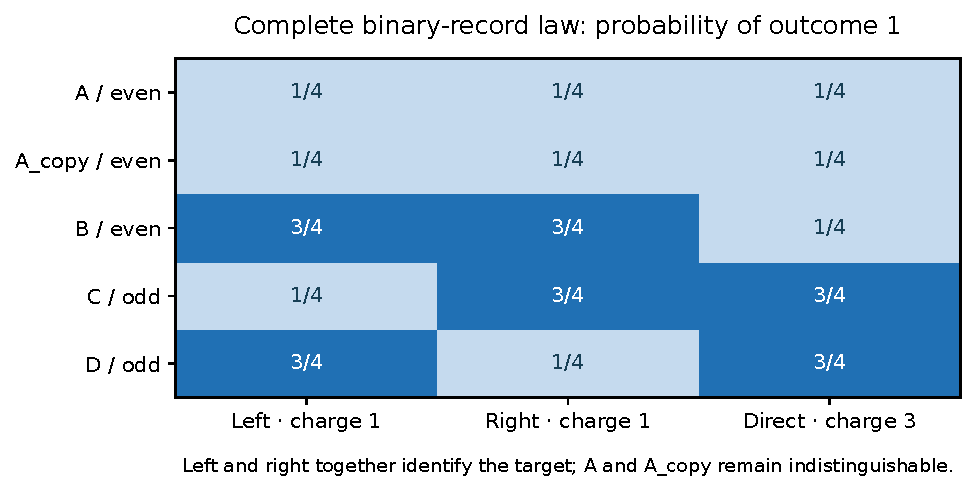
\includegraphics[width=0.88\textwidth]{suite_laws.pdf}
\caption{The complete laws in the finite-menu tutorial. The selected pair of probes resolves the target label while leaving two mechanisms indistinguishable. Every displayed probability is specified analytically.}
\label{workflow:figure}
\end{figure}

Set every whole-record TV radius to $1/100$ and the sampling failure budget to $1/20$. The robust gaps are $12/25$, the selected sampling radii are $3/25$, and the implementation allocates 278 records to each of the two experiments: 556 records in total. Deliberately synthetic frequencies near $1/4$ for both probes retain A and A copy and report ``even''. The complete mechanism remains unidentified. If both TV radii of a pair increase to $1/4$, its nominal half-unit contrast no longer gives positive separation; the robust menu reports the unresolved pairs.

Run the example after installation:
\begin{verbatim}
python examples/suite_tutorial.py --output results/suite_tutorial.json
\end{verbatim}
The JSON includes every nominal law, radius, selected event, record count, retained model and limitation. The supplied counts are synthetic and test the inference interface; they are not simulated discoveries or laboratory measurements.

\section{Using a result in the laboratory}
A useful deployment proceeds through one chain of evidence. First write the physical contract and the target. Then test structural access: either produce an equivalence certificate or generate a candidate experiment. Next verify that calibration leaves a nonzero target-relevant gap. Choose the statistical objective and repetition or feedback policy, and translate the proposed operations into a complete resource ledger. Execute the protocol only after this mapping is justified. Finally retain the models or target values compatible with the actual records, and report abstention or model failure when required.

A result becomes transferable when another group can substitute its calibrated model, run the same checks, execute the returned protocol, and reproduce the promised target coverage or error rate. Different laboratories need not share microscopic mechanisms. They must share the mathematical interface and justify its assumptions for their apparatus.

The next extensions should preserve that standard. Continuous parameter families require validated optimization or analytic envelopes. Large quantum devices require locality, sparsity or other justified structure. Nonstationary experiments require conditional predictions or explicit drift models. Resource comparisons require matched objectives and complete physical accounting. These are clear mathematical and experimental tasks, rather than claims already established by the finite examples.

\chapter{The reference implementation}
\label{toolkit:chapter}

The accompanying package turns a precisely specified comparison into a
portable algebraic certificate and a complete experimental plan. Its public
entry point begins with the scientific question, the two target labels, the
available interventions, and the preparation. The program does not infer
these ingredients from a dataset. A scientist supplies them and can inspect
every consequence reported by the calculation.

Version 0.10.0 retains a strict JSON workflow for two finite classical
instruments with rational coefficients. A second, Python-level interface
exposes finite linear representations, continuous-time approximation,
bounded adaptive design, and sequential model checks. These interfaces have
different hypotheses; their availability in one package does not silently
extend the scope of the JSON workflow.

\section{Install and run the first comparison}

From the root of the released reference package, use Python 3.10 or later:
\begin{verbatim}
python -m pip install .
constructive-access analyze examples/passive.json -o passive-report.json
constructive-access analyze examples/active.json -o active-report.json
constructive-access verify examples/active.json active-report.json
\end{verbatim}
The installation requires SymPy and mpmath. The portable algebra checker itself uses
only Python's standard library. For an existing environment with the
dependencies installed, the same commands are available through
\texttt{python -m constructive\_access}. No code imports from an earlier
research directory or requires an unreleased local file.

The passive example has two hidden states, initial distribution
$(1/2,1/2)$, and the same state-revealing read operation under each candidate.
All passive transcript laws coincide. The program returns an exact
equivalence certificate; collecting more passive records does not change
that model conclusion.

The active example also permits an unobserved drive. Its transition matrix
has both rows equal to $(3/4,1/4)$ under candidate 0 and $(1/4,3/4)$ under
candidate 1. Reading costs one operation, driving costs two, and fresh
preparation costs one additional operation per complete record. The
least-action-charge distinguishing experiment is drive followed by read.
It has action charge 3 and total declared charge 4 per record. Its complete
two-outcome laws are
\[
 P_0=(3/4,1/4),\qquad P_1=(1/4,3/4).
\]
The reported total variation is $1/2$ and the one-record equal-prior Bayes
error is $1/4$. The outward-rounded affinity calculation certifies 12
independent complete records as sufficient for average error at most
$1/10$, with declared batch charge 48. This is a sufficient count, not a
minimum sample count. Neither the operation charge nor its minimum is a
measured energy consumption.

The witness contains an action--outcome word, but the implemented experiment
retains \emph{all} outcomes of the associated action sequence. A drive is
not repeated for free until a desired outcome occurs. The report lists the
complete normalized law, making that distinction inspectable.

\section{What a contract contains}

\texttt{load\_contract} accepts a file path, a JSON-compatible mapping, or a
validated contract. It rejects floating-point model coefficients, duplicate
JSON keys, unsupported fields, invalid probability kernels, negative
charges, and mismatched action/outcome alphabets. Integers and exact
rational strings such as \texttt{"1/3"} are accepted. Decimals written as
strings are interpreted as the exact rational number they specify, without
a claim that the physical coefficient is exact.

Each contract contains the following information:
\begin{itemize}
\item A question, target name, and two distinct target labels, ordered with
the candidate models.
\item Two normalized classical instruments: a row initial distribution and
one nonnegative substochastic matrix for each recorded outcome of each
action. Outcome matrices sum to a row-stochastic matrix for each action.
Missing probability mass must be represented by an explicit recorded
outcome, such as abort.
\item A declared additive action charge, units, resource interpretation,
per-record overhead, calibration statement, and included and excluded
items. Energy is an allowed interpretation of a calibrated bound, never
an inference from the word length.
\item A preparation description and an explicit declaration of whether
complete records are independently and identically prepared.
\item A desired equal-prior average error, rational precision settings, and
a cap on explicit transcript enumeration.
\item Optionally, a deterministic finite automaton restricting complete
action sequences. Its transitions cannot depend on postselected outcomes.
\item Optionally, a whole-record total-variation calibration radius for
each candidate, a joint calibration failure probability, and the stated
justification for those inputs.
\end{itemize}

The canonical contract hash binds these assumptions and target meanings to
the report. It identifies the supplied specification. It does not establish
the provenance of a physical calibration, authenticate a laboratory, or
prove that the candidate family contains the true mechanism.

\section{Separate synthesis from checking}

The Python entry points are:
\begin{verbatim}
from constructive_access import load_contract, analyze, verify_report

contract = load_contract("examples/active.json")
report = analyze(contract)
verification = verify_report(contract, report)
assert verification["verified"]
\end{verbatim}
Analysis builds a paired linear representation, runs an exact
charge-priority span search, exports its filtered closure identities, and
checks them. A witness is minimal in the lexicographic order
\((\hbox{additive action charge},\hbox{word length})\).
The report checker independently reconstructs the paired model from the
caller-supplied contract and checks every required expansion identity.
It does not rerun the witness search, compute ranks, or trust the
synthesizer's history. It then reevaluates the complete selected experiment
and its reported statistical quantities. Modified conclusions, unsupported
fields in the report, altered probabilities, missing closure identities,
and certificates for a substituted model fail this check.

There are three distinct mathematical outputs. An equivalence certificate
proves equality for every permitted finite protocol in the declared model.
A witness proves a nonzero probability contrast. A finite-error bound
provides a sufficient number of repeated complete records under its stated
sampling assumptions. A nonzero contrast is not perfect discrimination.

The transcript cap is a computational guard, not an observability theorem.
If explicit enumeration exceeds it, the program retains the exact access
certificate and returns \texttt{transcript\_limit\_exceeded}; it does not
issue a statistical plan. If iid preparation is not declared, the program
reports one-record quantities without a repeated-record guarantee.

\section{Calibration can change the operational answer}

Run the uncertainty example with:
\begin{verbatim}
constructive-access analyze examples/calibrated.json -o calibrated.json
constructive-access analyze examples/calibration_gap_closed.json
\end{verbatim}
The first example assumes whole-record TV radii $1/100$ under both
candidates and a joint calibration failure probability $1/100$. These are
illustrative assumptions, not measurements. For the event
$E=\{y:P_0(y)>P_1(y)\}$, the program evaluates
\[
 a=\max\{0,P_0(E)-r_0\},\qquad
 b=\min\{1,P_1(E)+r_1\},\qquad g=a-b.
\]
When $g>0$, classify using the empirical event frequency with threshold
$(a+b)/2$. Conditional on pre-acquisition calibration information, each
fixed actual hypothesis must produce iid classification records. A
simultaneous calibration event certifies the corresponding conditional
whole-record laws. Classification records cannot be reused to choose or
calibrate the event or threshold.

For a conditional error allocation $\alpha$, the exact implementation
chooses an integer $M$ satisfying
\[
 \frac{Mg^2}{2}\ge L\ge\log(1/\alpha).
\]
Here $L$ is a rational upper enclosure obtained by range reduction and the
positive series
\[
 \log x=2\sum_{k=0}^{n-1}\frac{z^{2k+1}}{2k+1}+R_n,
 \quad z=\frac{x-1}{x+1},\quad
 0\le R_n\le\frac{2z^{2n+1}}{(2n+1)(1-z^2)}
\]
after reducing $x$ to $[1,2]$. Hoeffding's inequality gives a conditional
error at most $\alpha$ for each hypothesis. Adding the stated joint
calibration failure probability gives the unconditional bound. There is no
claim that this conservative event test is optimal.

The supplied example has $g=12/25$, threshold $1/2$, and $M=21$. Its
conditional allocation is $9/100$, and the unconditional bound is
$1/10$. Declared batch charge is 84 operations, including the stated
preparation overhead. The negative control increases both radii to $1/4$;
the robust gap closes and the program returns
\texttt{calibration\_gap\_not\_certified}. This failure concerns the
specified uncertainty certificate. It does not prove that every possible
physical experiment fails.

\section{Advanced interfaces and their boundaries}

The top-level Python package also exposes the following preserved
implementations:
\begin{description}
\item[Finite instruments.] Use \texttt{RationalInstrument} for a normalized
classical instrument. Use \texttt{LinearRepresentation} for a general
weighted representation, and \texttt{ActionDFA} for an action grammar.
The functions \path{compare_models}, \path{minimum_cost_witness}, and
\path{experiment_law} support direct finite-model work. A signed linear
representation is not automatically a physical quantum instrument; a
separate complete-positivity and normalization justification is required.
\item[Continuous time.] \texttt{certified\_wait} encloses a finite CTMC
transition by an exact rational stochastic approximation and a row-TV
error. \texttt{protocol\_tv\_radius} and
\texttt{robust\_word\_gap} propagate the stated approximation error.
Equality of approximate transition laws cannot prove equality of the true
continuous-time laws.
\item[Adaptive design.] \texttt{optimal\_design} optimizes the declared
two-hypothesis classical Bayes risk under a finite integer budget and a
mandatory finite horizon. \texttt{best\_fixed\_design} supplies a matched
open-loop comparison. These routines do not optimize arbitrary quantum
policies or unknown physical models.
\item[Sequential adequacy.] \texttt{AdequacyMonitor},
\texttt{Interval}, and \texttt{interval\_bet} maintain e-process evidence
against declared conditional predictive envelopes. Their validity requires
the appropriate conditional predictions at every step; stationary marginal
intervals cannot be substituted.
\item[Linear targets.] \texttt{identify\_linear\_target} checks the
row-space criterion for a known fingerprint matrix.
\texttt{minimax\_certificate} and
\texttt{verify\_minimax\_certificate} compute and check exact
primal--dual recovery bounds for small rational instances over the full
positive parameter orthant with a coordinatewise deterministic error box.
The generator uses vertex enumeration and is not presented as a scalable
general linear-programming solver.
\item[Counting-channel energy.] \texttt{count\_cap} and
\texttt{verify\_count\_cap} produce and check a rational Chernoff
envelope under a separately supplied predictable compensator bound.
\texttt{declared\_energy\_cap} combines a checked count cap with a
gross-work-per-event bound and an apparatus bound in the same physical
unit. The compensator, work, and apparatus assumptions must be justified
separately from observation-law calibration.
\end{description}
The finite-family experiment-suite workflow is described separately in this
reference. It addresses target-specific design across multiple candidates;
the two-model JSON command remains deliberately explicit about its smaller
input class.

For a concrete linear recovery example:
\begin{verbatim}
from constructive_access import minimax_certificate, verify_minimax_certificate

F = [[1, 1], ["1/2", 1]]
b = [1, 0]
epsilon = ["1/100", "1/100"]
certificate = minimax_certificate(F, b, epsilon)
assert certificate["absolute_error"] == "1/25"
assert verify_minimax_certificate(F, b, epsilon, certificate)["verified"]
\end{verbatim}
This deterministic minimax guarantee assumes a known intervention response
matrix and the specified full error box. It does not certify that a
biochemical reporter implements the declared selective intervention.
For a counting-channel illustration, \texttt{count\_cap(10, "1/100")}
returns 22. With gross event work at most $3/2$ and apparatus work at most
4 in the same unit, the conservative declared energy cap is 37. The example
does not establish those physical input bounds from sensor data.

\section{Reproduction and provenance}

The package contains source-level provenance for every preserved module in
\path{constructive_access/_vendor/PROVENANCE.json}, including the
original SHA-256, the vendored SHA-256, and any import-path substitution.
Source copies are independent of earlier release directories. No software
license is invented or implied by this packaging step.

The workflow tests exercise passive equivalence, active witnesses, charge
minimality checking, zero-charge actions, action grammars, complete
transcript normalization, calibration gap closure, non-iid declarations,
enumeration limits, malformed exact inputs, report forgery, model
substitution, and command-line failure handling. The independent review
tests supplement these with separately derived examples. Run the complete
original workflow test collection using:
\begin{verbatim}
python -m unittest discover -s tests -v
\end{verbatim}
Passing these checks establishes reproducibility for the supported software
contracts. It does not establish a sensor calibration, a successful
laboratory intervention, an unmodeled dissipation estimate, or community
acceptance of the proposed framework.

\section{Response and access-completion modules}
The \path{constructive_access.completion} subpackage adds six modules:
\texttt{physical\_access}, \texttt{quantum\_completion},
\texttt{pulse\_test}, \texttt{graph\_access},
\texttt{robust\_completion}, and \texttt{composition}.
Their contracts and examples appear in the corresponding chapters.
\begin{verbatim}
python examples/completion_tutorial.py \\
    --output results/completion_tutorial.json
python verify.py
python research/clean_reproduction.py
\end{verbatim}
The first command uses the installed package to verify the qubit response
threshold, construct the calibrated three-arm test, and certify both an
energy lower and upper bound of 6400 in the declared model units. The full
reproduction additionally runs producer tests and separate adversarial checks,
regenerates exact certificates and numerical illustrations, and builds this
reference. The clean reproduction builds an offline wheel, installs it in a
separate environment, and checks scientific outputs against the source run.
The software can check a supplied physical contract; it cannot establish an
apparatus calibration or an experimental result by executing a model.

\section{Calibrated explanations and sequential experiments}
The \path{constructive_access.robust} subpackage adds exact physical response
bounds, protected clock design, fixed and anytime statistical tests, and
counts-to-explanation inference. Run the complete installed example with
\begin{verbatim}
python examples/robust_tutorial.py --output results/robust_tutorial.json
\end{verbatim}
The explanation routine receives an already specified preparation, detector,
clock and calibration contract. Its synthetic demonstration is labeled in both
source and output. For actual data the record count must be fixed before
collection, or the separate time-uniform inference method must be used.
The sequential betting fraction and null envelope must be selected before the
current random preparation arm and clock are drawn. Marginal clock agreement
without independence from the physical trajectory is insufficient.

The same example certifies the arbitrary-preparation realization-size witness
and its 6000-record four-arm design. The functions
\texttt{encode\_dimension}, \texttt{dimension\_plan}, and
\texttt{verify\_dimension} preserve the distinction between a complete
witness-error radius and a single arm's error. The quantum certificate uses
exact rational preparations and an independently checked open-system model.


\section{Classical realization and thermodynamic certificates}
The \path{constructive_access.frontier} subpackage exposes five separate
contracts: \texttt{hierarchy}, \texttt{spectral}, \texttt{limits},
\texttt{thermodynamic}, and \texttt{energy\_certificate}. Run their installed
examples together with
\begin{verbatim}
python examples/frontier_tutorial.py --output results/frontier_tutorial.json
\end{verbatim}
The tutorial checks three finite-noise state requirements, an Erlang-clock
certificate, a matching cyclic classical model, a reversible approximation,
a synthetic-count entropy bound, and the continuous-moment curvature witness.
These are different access contracts, not interchangeable black-box tests.

For example, the following inference accepts two predeclared independent-pair
counts. The numbers below are synthetic:
\begin{verbatim}
from fractions import Fraction as F
from constructive_access.frontier import thermodynamic

result = thermodynamic.from_counts(
    5000, 2560, 5000, 3680,
    F(1, 50), F(1, 20), F(8, 5), F(21, 10))
assert result["rate_lower"] > 0
\end{verbatim}
The two lags are $8/5$ and $21/10$ in declared time units, the one-sided
probability radius is $1/50$, and the joint sampling failure allowance is
$1/20$. An entropy interpretation requires stationary sampling, common
homogeneous dynamics, noninvasive fixed readout and ordinary time reversal.
Sampling counts do not validate those physical assumptions.

For a positive-integer lag menu, \texttt{energy\_certificate.certify} accepts
simultaneous probability intervals and positive rational scores. Its exported
certificate records all inputs, a continuous polynomial normalizer bound and
a directed lower bound on relative-entropy separation. The function
\texttt{verify} recalculates that certificate against separately supplied
inputs. It is a deterministic recheck, not a second proof implementation.
Independent tests separately check generator models and polynomial bounds.
The optional \texttt{design} score proposer requires NumPy and SciPy; it is
followed by exact continuous-domain checking. A failed or weak proposal cannot
be interpreted as evidence of equilibrium.

The complete cumulative test and figure collection is run by
\texttt{python verify.py}; \texttt{--skip-pdf} omits typesetting only.
Source provenance binds all five packaged modules to their preserved phase
sources. No previous release directory is required. None of these certificate
functions discovers an apparatus's hidden-state count, reversal parity or
thermodynamic embedding from an undeclared dataset.


\section{Virtual laboratories and apparatus-aware inference}
The \path{constructive_access.virtual} subpackage adds exact contrast and
dependent-record confidence interfaces, timing and exposure controls, and
numerical laboratories for thermodynamic and qubit experiments. Simulations
require the optional numerical dependencies:
\begin{verbatim}
python -m pip install '.[simulation]'
python examples/virtual_tutorial.py --output results/virtual_tutorial.json
\end{verbatim}
The tutorial exercises the installed mathematical interfaces without replaying
the production simulations. The complete frozen simulation contracts are in
\path{virtual/contracts}. Standalone producer scripts and raw retained records
are in \path{virtual/code} and \path{virtual/results}. A full
\texttt{python verify.py} replay regenerates all model experiments, matched
comparisons, exact countermodels, figures and the reference. The separate clean
reproduction installs a wheel and compares scientific outputs byte for byte.

All parameters in these virtual laboratories are illustrative. The simulator knows a hidden
mechanism to evaluate coverage and power; the inference functions do not receive
that mechanism. Exact concentration certificates, numerical physical evolution,
Monte Carlo intervals and measured physical evidence are separately labeled.
Chapter~\ref{ch:ci-empirical} separately reanalyzes published measurements;
those data are included with attribution and an explicit inference limit.

\section{Calibrated inference and public-data reanalysis}
The \path{constructive_access.calibrated} subpackage supplies calibrated
moment supports, nonlinear certificates, activity bounds, dissipation
countermodels, sequential replay, common-block confidence and bounded analog
inference. Run the installed tutorial with
\begin{verbatim}
python examples/calibrated_tutorial.py --output results/calibrated_tutorial.json
\end{verbatim}
Each function retains its own physical and sampling contract. In particular,
stationary marginal records, independent pairs, dependent common blocks and
predictable batches do not share interchangeable confidence corrections.
The nonlinear primal upper bound concerns an observational relaxation, not
an upper bound on physical entropy production. A null upper endpoint in the
resolved-jump entropy helper means positive infinity.

The empirical extra installs HDF5 support. The three licensed, unmodified
measurement files live in \path{calibrated/data/source_audit}; the wheel does
not embed them. Standalone loader and analysis commands reproduce the data
audit and exploratory analysis without network access. Hash and schema
checks precede numerical reads. Neither embedded Python objects nor pickled
force models are evaluated. The empirical chapter records which unavailable
calibrations prevent a thermodynamic certificate.

\chapter{Research lineage, scope, and routes to application}
\label{researchmap:chapter}

\section{The subject and its place in existing science}

Constructive access concerns a concrete experimental question: given a target
property, a class of possible mechanisms, and an apparatus, which conclusions
can be justified, and what additional experiment would justify more?
The apparatus includes preparation, interventions, timing, detection, retained
records, and resource limits. Its mathematical object is the family of
transcript laws produced by the permitted protocols. This formulation supplies
a common language for systems whose underlying physics can be quite different.

This subject lies at the intersection of system identification, statistical
decision theory, controlled stochastic models, quantum characterization, and
thermodynamic inference. Each has a substantial history. Aggregated Markov
models and their indistinguishable realizations were studied in ion-channel
kinetics \cite{p_kienker,p_larget}. Finite linear representations and equivalence
algorithms originate in automata and realization theory
\cite{f_tzeng,f_kiefer,f_thon}. Observable operator models and predictive state
representations already replace inaccessible coordinates by predictions of
future experiments \cite{f_jaeger,f_littman}. A predictive coordinate need not
name a unique molecule, hidden conformation, or physical degree of freedom.

The classical--quantum linear correspondence is also established. Quantum
finite-state equivalence uses finite-dimensional operator spaces
\cite{f_wang,p_faigle}; a recent unified treatment constructs canonical
generalized hidden Markov representations for classical and quantum models
\cite{p_riechers}. The present use of an accessible effect space inherits that
lineage. Similarly, risk-based comparison of experiments and optimal recovery
provide established foundations for deciding which distinctions matter and
how errors limit recovery \cite{f_blackwell,p_donoho}.

The contribution developed in this reference is an explicit chain from those
foundations to a checkable experimental conclusion. A user specifies a
physical access model and a target; obtains an obstruction or a distinguishing
protocol; verifies its algebraic certificate; assigns calibration and sampling
errors; and states the physical resource boundary under which the conclusion
holds. The same chain includes abstention when the supplied model class fails
or the remaining models disagree about the target. The particular model
results and software artifacts are useful parts of that chain. Their status
is recorded separately from the established general principles.

\section{How the earlier results fit together}

The initial boundary question asked when a local observation must display an
arrow of time inherited from driving elsewhere. A finite ring made the
boundary mechanism explicit: one connection carries the driving, while a
binary detector reports a region. This separated three targets that an
informal arrow-of-time argument can conflate: a driven hidden dynamics,
irreversibility of the recorded process, and incompatibility of that recording
with every equilibrium explanation.

In the four-state adjacent-region example, the recording can be reversible
even when the ring is driven; on the specified reciprocal branch an explicit
equilibrium realization produces the same complete recording. Larger-ring
classifications, detector placement, and weak-drive response orders then
showed that access depends on geometry and acquisition. Retaining timestamps
or changing readout spacing can change the leading information order without
changing the hidden physical process. These are exact classifications of the
stated models, rather than statements about the existence of time.

The next step changed access through interventions. In the driven triangle,
each constant-control singleton record is blind to current orientation,
whereas a sequence of two controls produces a current-dependent return
contrast. An autonomous reversible kinetic gate provides a second route: a
binary three-time correlation acquires a leading term proportional to the
controlled edge current and the gate profile's Dirichlet form. The gate's own
steady channel entropy contribution can vanish while the source remains
driven. Preparation, sensing, and control implementation still require their
own accounting.

The quantum branch showed why the target must remain explicit. For the
specified three-site chain, one family of central instruments conceals the
bias magnitude, while a larger family exposes it. Reflection symmetry still
conceals the sign under every permitted central-only protocol. A calibrated
spatial asymmetry changes that conclusion. Magnitude, orientation, and a
complete microscopic model are different identification tasks.

The finite-instrument formulation subsequently provided a common algebraic
interface for these examples. Its cost certificates concern the cheapest
nonzero witness under a prescribed additive charge. Robust testing and
finite-budget decision design concern reliable inference. These objectives
require separate calculations: a very cheap nonzero witness may have much
worse reliable-decision cost than a more informative experiment.

The channel-resolved application studies expose a further distinction between an
inaccessible state and an inaccessible transition channel. Two reaction
mechanisms can have the same full state generator yet different physical
currents and dissipation. Adding the same state-level control preserves that
equivalence. A calibrated channel-selective intervention can remove it in the
worked two-channel model. This is a more precise rule for choosing access
than the suggestion that any temporal modulation reveals hidden dynamics.

Table~\ref{researchmap:lineage} summarizes the retained role of each stage.
The machine-readable provenance record binds individual inherited claims to
their source and result hashes; the table is a reading map, not a count of
discoveries.

\begin{table}[htbp]
\centering\small
\begin{tabular}{p{0.23\textwidth}p{0.67\textwidth}}
\hline
Stage & Retained contribution to the reference\\
\hline
Boundary and detector models & Explicit source, sensor, equilibrium mimics,
sampling effects, and response-order examples.\\[2pt]
Controlled hidden currents & Interventions that alter observable distinction;
control placement and preparation failure cases.\\[2pt]
Autonomous equilibrium gate & Current--correlation identity, triangle
activation criterion, and the cost of hiding the controller record.\\[2pt]
Finite instruments & A common exact representation, finite equivalence
test, witness synthesis, and bounded decision design.\\[2pt]
Certification and adequacy & Independently checked cost certificates,
conditional prediction tests, calibrated abstention, and energy tails.\\[2pt]
Physical diagnostic models & Selective channel identification, targeted
quantum diagnosis, fixed-nuisance sensing, and hidden-energy obstructions.\\
\hline
\end{tabular}
\caption{The dependency structure of the research. Each row supplies a
different part of the experimental argument.}
\label{researchmap:lineage}
\end{table}

The subsequent stages extend this chain in two directions. Compatible-model
results turn evidence into requirements on hidden state count, preparation and
sustained dissipation, with explicit equilibrium countermodels. The virtual
laboratories establish how timing, detector exposure and serial dependence
alter those certificates. The calibrated-inference chapters then improve
statistical use of detector moments, analog records and sequential acquisition,
while proving limits on total-dissipation reconstruction. Their joint
calibration test treats the extra measurement directly as part of the final
scientific contrast. The public-data chapter tests this chain against an
actual observation format and records precisely where calibration remains
insufficient.

\section{What is established, and what is specific to this work}

Three-time correlation tests of nonequilibrium and current inference predate
this work \cite{physics-qian}. Equilibrium kinetic coupling can also carry trajectory
information \cite{p_barato}. The specific gate result here is the factorized
coefficient, its controlled assumptions, the triangle converse, and the stated
information-order comparison. The general-network coefficient supplies a
sufficient activation condition; a vanishing coefficient need not imply
complete invisibility. Historical priority for this precise combination
remains open.

The independent cost checker verifies explicit filtered closure identities,
including those needed to exclude every cheaper word. Its useful distinction
is the exported proof obligation: a user can check the claimed objective
without trusting the search history. Exact equivalence, invariant-space
certificates, and weighted witness methods already exist
\cite{f_kiefer,f_thon}. The implementation does not establish that its supplied
matrices describe an apparatus, nor does it convert arbitrary charges into
joules.

The adequacy layer uses established nonnegative betting processes
\cite{caWaudbySmithRamdas2024,p_intervals}. Its application obligation is to supply valid
conditional prediction envelopes under the actual interventions and histories.
That is stronger than supplying stationary averages. The selective-response
criterion and its deterministic error bounds use linear identifiability and
optimal-recovery geometry. Their exact certificates make the assumptions and
the amplification of calibration error visible.

Recent thermodynamic inference already extracts kinetic information from
partially observed transitions, including periodically driven systems
\cite{p_maier}. Care is needed when applying thermodynamic time reversal after
coarse observation: a physically justified reversal operation and a defined
observation map are part of the model \cite{p_dieball}. This reference's
instantaneous finite-state detectors have an explicit reversal convention;
extensions to milestoned, filtered, or history-dependent detector outputs
must re-establish the relevant correspondence.

Adaptive quantum design also has experimental precedents
\cite{p_stace,physics-bonato}. The worked quantum and Ramsey calculations here
provide transparent small models, explicit alternative hypotheses, and
matched decision objectives. They are reference calculations against which
an implementation can be checked. Demonstrating a hardware advantage
requires comparison with appropriate existing methods on the same device.

\section{A practical standard for extending the subject}

A new application should identify the target before selecting its mathematics.
For a current, the target must name the physical channel and its units. For a
quantum fault, it must name a justified error dictionary and the operations
permitted during diagnosis. For a sensor, it must specify whether the task is
sign discrimination, local parameter precision, tracking, or a decision with
unequal consequences. For energy inference, it must state whether the target
is native-channel free-energy dissipation, gross supplied work, or total
apparatus consumption.

The minimum useful transfer includes a negative control. Examples are a
channel decomposition that produces the same state record, a control family
that preserves a quantum symmetry, an insufficiently selective intervention,
or a missing candidate that forces abstention. A successful case should then
change exactly the access assumption responsible for that failure and predict
the resulting effect before evaluating new data.

Four external milestones would establish practical maturity in a new setting:
\begin{enumerate}
\item An independent specialist checks the theorem, the software contract,
and the closest prior methods for the stated model class.
\item Independent calibration and physical measurements test the preparation,
intervention, detector, memory, and resource assumptions.
\item A comparison holds the scientific objective, error criterion, and full
resource boundary fixed; an increase in contrast alone is insufficient.
\item A second implementation or apparatus reproduces the prediction and
tests at least one intended transfer beyond the development example.
\end{enumerate}
These are measurable acceptance conditions. The present release supplies
mathematical derivations, executable models, and internal adversarial checks.
It also includes the exploratory published-data reanalysis in
Chapter~\ref{ch:ci-empirical}, which identifies concrete apparatus-calibration
gaps. It contains no new laboratory measurements, empirical entropy
validation or external peer-review decisions.

\section{Extensions with a clear scientific payoff}

Several extensions now have a precise starting point. A validated nonlinear
response family can replace the linear selective-response model, provided
identifiability and uncertainty propagation are proved for that family.
Chapter~\ref{ch:continuous} supplies a finite CTMC adapter. Extensions
beyond that finite-model, finite-menu contract to continuous controls or
infinite-dimensional dynamics must also carry approximation error into
the final decision bound, rather than report only solver tolerance. A structured many-body
model can reduce computational burden, provided the structure is physically
justified and the bound includes deviations from it. Detector memory, drift,
and correlated preparation can be handled by enlarging the state or by
conditional envelopes that actually cover those effects.

Chapter~\ref{completion:composition} now supplies a finite classical composition contract and a constructive deterministic interface refinement. Beyond that scoped result, composition remains a concrete research direction. Individually
uninformative components can become informative when the allowed coupling
changes their transcript laws; combining records that remain jointly
equivalent cannot do so. A useful composition theorem must specify the joint
preparation, shared hidden variables, allowed couplings, and target. This
distinguishes a real increase in experimental capability from merely adding
more components or more processing.

The broad claim is therefore an operational one: scientific conclusions can
be organized around what specified experiments preserve, erase, and expose.
The constructive finite theory makes a substantial part of that question
computable and reviewable. Further generality is earned by extending those
interfaces and proving their contracts, with the physical interpretation
checked in each new setting.

\section{Relation to earlier work and the next physical test}
\label{sec:completion-positioning}

The contribution of access completion is a chain of usable certificates:
identify an inaccessible target, specify the additional physical operation,
bound what its data can establish, and expose the assumptions under which the
conclusion fails. Several links in this chain are established mathematics.
Separating those foundations from the results derived here makes the proposed
physical test easier to assess and reproduce.

\paragraph{Established foundations.}
Conservation-law sensor placement, spanning-tree constructions, cost, and
precision constraints have a substantial earlier
literature~\cite{ac_bagajewicz,ac_he,ac_xu}. The cotree and target-cut results
are explicit network-flow specializations. Perturbation design based on
graph-theoretic identifiability also predates this work~\cite{ac_gross}.
Target-specific allocation belongs to optimal experimental
design~\cite{ac_elfving,ac_harman}; adding resource constraints to terminal cuts
has established complexity consequences~\cite{ac_aissi}. The particular
calibration-floor objective studied here therefore requires its stated error
model and direct proof. It is not a universal thermodynamic energy law.
Likewise, lumpability and approximate trace guarantees underpin the classical
interface construction~\cite{ac_buchholz,ac_bian}. Quantum equivalence under
composition has its own established theory~\cite{ac_lalire,ac_deng}.

\paragraph{The precise response result.}
Stationary barrier-response identities are
established~\cite{ac_aslyamov_response,ac_aslyamov_static}.
Finite-amplitude stationary formulas already include parallel physical
channels~\cite{ac_bao_nonlinear}; transient response relations are also
available~\cite{ac_zheng}. Monotonicity of a stationary response as a barrier
strength varies~\cite{ac_floyd} concerns a different variable from the pulse
duration used here. First-passage response theory supplies further close
connections~\cite{ac_liang_budget,ac_bao_firstpassage}.

The candidate extension is the following all-time statement. Starting from
native stationarity, suppress one bidirectional physical channel by a fixed
factor $r<1$ while holding the other rates fixed. For a singleton endpoint
detector, the response factors as
\begin{equation}
 \Delta p_j(t)=-(1-r)J_e H_{ij}^{r}(t),
 \qquad H_{ij}^{r}(t)>0\quad(t>0).
\end{equation}
The first-hit proof uses the strong Markov property and ordinary occupation
potentials, within established Markov potential theory~\cite{ac_coolen}.
Its useful consequence is a current-sign certificate at every positive pulse
duration, with explicit bounds using only endpoint exit-rate ceilings.
It does not require reconstructing the hidden network. A protected coarse
detector also qualifies when a separately justified entrance-gateway condition
holds; arbitrary aggregation does not preserve the conclusion.

The driven-qubit calculation gives an exact parameter boundary at which this
classical response restriction fails. Connections between coherent dynamics
and failure of classical stochastic descriptions are already well
developed~\cite{ac_smirne,ac_prech}. Here the distinguishing feature is the
specified intervention and endpoint-response inequality. The result rejects
the calibrated classical model class; its assumptions cannot be inferred
from two response averages alone.

\paragraph{Priority and evidence limits.}
The proofs and computational certificates establish the stated mathematical
claims within their models. They establish neither historical priority nor
laboratory performance. The particularly close sensor-design article by
Prakash~\cite{ac_prakash} was available only through primary metadata and
indexed excerpts in this audit. The higher-cumulant response article of Bao
and Liang~\cite{ac_bao_higher} was inspected at abstract level only. Their full
texts remain necessary overlap checks. The search of older finite-time
potential-kernel results is also incomplete. A detailed source map records
which full texts, sections, or abstracts were inspected. These physical-response examples have no new empirical validation or external
peer-review decision. Chapter~\ref{ch:ci-empirical} separately reports an
exploratory reanalysis of published optical-tweezer measurements.

\paragraph{The next validation gate.}
The highest-leverage physical test is a controlled two-level platform with
independently adjustable incoherent excitation and decay channels. It should
first establish stationary preparation, population-readout calibration and
leakage bounds; then independently verify that the pulse rescales both rates
of the selected channel while leaving the Hamiltonian and other channels
within declared tolerances. This calibration is part of the experiment,
not an assumption justified by fitting the desired sign reversal.

The measurement then compares native and pulsed endpoint populations at two
prespecified durations, with randomized acquisition order and independent
repreparation. The incoherent control should obey the classical sign
restriction. Increasing the calibrated coherent-drive ratio across the
derived threshold should produce the predicted reversed response. Sampling,
preparation, drift, detector, and intervention error budgets must be small
enough that the two response intervals exclude zero with opposite signs.
Repeating the experiment with deliberately nonselective control or coarse
readout tests the documented failure modes rather than merely reproducing
the favorable case.

Passing this gate would validate a practical way to test a structural model
assumption using a small set of interventions. It would also determine which
parts of the calibration dominate sensitivity. A failure would locate a
specific mismatch between the physical platform and the model. Either
outcome is more informative than projecting the framework directly onto
unresolved problems of large-scale computing or biological flux.

\section{Positioning and physical interpretation}

The principal extension in this phase is a quantitative treatment of a
coarse detector whose natural entrance distribution need not coincide with the
reference preparation. A departure from ideal occupation ordering then has a
measurable consequence: any admissible classical explanation must provide enough
entrance mismatch, sufficiently rapid crossings of the observed boundary, or
both. The comparison is against a specified set of physical capabilities, rather
than against a fitted list of hidden networks.

Let $B$ be the detected region, let the reference preparation lie in $B$, and let
the comparison preparation lie outside it. Write $H(T)$ for the difference of
their expected cumulative occupations in $B$. In the reset-conditioned theorem,
$\eta$ bounds the total-variation mismatch between the first-entrance law and
the reference reset law, conditional on the entrance time. With the stated
uniform entry and exit intensity bounds $a,b$, define
\[
 A_c(T)=\int_0^T e^{-ct}\,dt,\qquad
 G_{a,b}(T)=\int_0^T e^{-bs-a(T-s)}\,ds.
\]
The sharp envelope is
\[
 H(T)\ge G_{a,b}(T)
 -\eta\{T-A_a(T)-A_b(T)+G_{a,b}(T)\}.
\]
Sharpness means attainability within the declared mathematical class; it does
not imply that an arbitrary apparatus realizes an extremizer. If the braces
are positive, a calibrated upper confidence bound on $H(T)$ gives a necessary
lower bound on $\eta$ for any classical explanation satisfying the chosen rate
caps. It gives neither an upper bound on the actual mismatch nor a unique hidden
mechanism.

At $\eta=1$, the envelope reduces to
$H(T)\ge A_a(T)+A_b(T)-T$. This endpoint requires only the relevant survival
envelopes and remains valid for history-dependent and time-dependent classical
processes satisfying the conditional hazard bounds. The intermediate
$0\le\eta<1$ theorem additionally uses its stated reset and continuation
conditions; the broader endpoint scope must not be transferred to it without
those conditions. Here $a$ and $b$ are caps on crossing intensities. They are not
the average total jump activity, heat production, or energy expenditure.

Classical speed and no-jump bounds are established. Shiraishi, Funo and Saito
relate distributional motion to dissipation and dynamical activity
\cite{rrShiraishi2018}; Hasegawa and Nishiyama derive concentration and response
bounds using no-jump probabilities \cite{rrHasegawa2024}. The present inverse
problem concerns a difference between two occupation experiments, with an
explicit reset-defect parameter and a saturating construction. Coarse-grained
memory and its effect on inference are also established concerns
\cite{rrBlom2024}. No claim of historical priority follows from these
comparisons. The contribution offered for review is this particular sharp
envelope, its operational interpretation, and the calibrated implementation.

Physical use requires evidence for the caps over the histories and preparations
covered by the test. An observed mean switching rate is insufficient. A hidden
entrance distribution cannot generally be certified from a binary detector
alone; when independent reset information is unavailable, the $\eta=1$ envelope
is the applicable conservative alternative. Preparation errors, detector drift,
timing discretization and finite-sample uncertainty must be included before
inverting the bound. A violation excludes the calibrated class. It does not by
itself establish quantum dynamics or identify the failed assumption. No
apparatus-specific validation of these requirements has yet been performed.

\subsection{Dimension rather than an assumed reset interface}

A complementary interpretation replaces reset and rate information with a
bound on hidden state count. Let $C_0$ denote the contrast between two arbitrary
preparations measured immediately, and $C_T$ their contrast with the same binary
detector at an independent uniform time in $[0,T]$. Every common homogeneous
classical Markov realization with at most three states obeys
\[
 |C_0-C_T|\leq1.
\]
The detector may have any fixed state-dependent response probability in $[0,1]$.
Measuring the immediate contrast removes the need to assume perfect extremal
preparations. The protected-sign rule follows when $C_0=1$. A violating qubit
example and a four-state classical construction distinguish quantum
attainability from the minimum classical realization size at this scalar
statistic. They do not characterize the full quantum record or exclude
classical explanations of unrestricted size.

Dynamical dimension inference already has a substantial literature. In
particular, delayed-data and spectral methods establish classical/quantum
dimension separations \cite{rrWolf2009}, while repeated-operation null tests
provide experimentally implemented alternatives \cite{rrBialecki2024}.
Temporal memory witnesses also predate this work
\cite{rrBudroni2019,rrVieira2022}. The proposed distinction is a finite-window
integrated inequality with an exact three-state threshold and a four-state
construction, under its stated preparation and evolution assumptions. Historical
priority and an experimental advantage over these methods remain unresolved.

Those assumptions supply real information. With two unrestricted preparations,
general prepare-and-measure data can always use two classical messages
\cite{rrGallego2010}; the stronger state count here depends on requiring a
single homogeneous continuous-time evolution and a common detector. Hidden
controller or environmental states that affect the evolution belong in the
classical realization being counted.

\chapter{Relation to established results and the remaining contribution}
\label{ch:rf-positioning}

The useful question is not whether partial observations can hide a mechanism.
That obstruction is established. The question pursued here is what a finite,
calibrated temporal record forces \emph{every compatible model} to contain or
expend. The answer depends on the experimental contract: a common dynamics,
repeatable preparation, detector, accessible times and an explicitly stated
classical or quantum comparison class. These conditions belong to the theorem,
not merely to its interpretation.

The work combines three tasks that are often separated: exclusion of models
with too few states, exclusion of stationary equilibrium explanations, and
constructive examples showing when neither conclusion is justified. The
specific mathematical and computational results should be evaluated on their
own statements. A shared presentation does not establish a new physical law,
a complete classification of hidden dynamics, or priority over the literatures
below.

\section{State number, positive realization and finite records}

Wolf and P\'erez-Garc\'ia already derived dimension information from observable
dynamics, including noisy Hankel-rank witnesses and a damped-qubit example
with arbitrarily large classical dimension requirements \cite{rrWolf2009}.
Their spectral argument uses stochastic eigenvalue restrictions originating
in work including Dmitriev--Dynkin and Karpelevich
\cite{rfDmitriev1946,rfKarpelevich1951}. An unbounded classical--qubit gap or a
frequency-to-decay state bound is therefore established prior work. Statistical
detection matrices also infer observable stochastic dimension from noisy data
\cite{rfSuccar2024}.

The extra issue is \emph{positive realization}: a scalar signal can have small
ordinary linear rank while requiring a much larger probabilistic realization.
The established positive-realization literature makes this distinction
explicit \cite{rfBenvenuti2022}. A nonnegative matrix factorization is a
necessary condition for a finite temporal model; it need not supply a common
stochastic semigroup realizing every time. Conversely, a low ordinary rank
cannot certify a small positive realization.

Two finite-record constructions address this gap here. The random-clock
construction supplies a quantitative distance from all generators below a
specified state number, allowing unknown preparation, unknown fixed detector
and arbitrarily large hidden rates. It does not infer an exact pole. The
antichain construction uses a finite temporal probability matrix and an
explicit positive-noise margin. The conservative record count of the first
construction is part of its result; existence of a finite test does not imply
experimental efficiency.

The antichain ingredient has especially close precedents. The exact
support-based inverse-central-binomial bound follows from established Boolean
rank and nonnegative-rank arguments \cite{rfDeCaen1981,rfGillis2020} and has
already been applied to quantum preparation--measurement tables
\cite{rfShahandeh2024}. Heinosaari and collaborators use the same sinusoidal
matrix, up to normalization, to demonstrate unbounded quantum advantage; they
also establish a stronger exact rank for the seven-point instance
\cite{rfHeinosaari2024}. The candidate addition here is the analytic tolerance
for nonzero diagonal entries, its single repeated-channel temporal realization,
and a specified finite-count rejection rule. It is not the first sinusoidal
matrix, quantum advantage or application of Sperner's theorem.

Temporal memory and environment-dimension witnesses provide another relevant
body of work \cite{rrVieira2022,rfVieira2024}. Their measurement sequences can
be invasive. A fresh preparation with one endpoint measurement imposes a
different contract, so numerical comparisons require matching the operations,
reset assumptions and counted memory. Quantum counting-process precision is
also connected to finite memory \cite{rfOlamaei2026}; an external randomized
endpoint clock is not itself a first-tick counting process.

\section{Classical approximation identifies the limit of the contract}

The Poisson smoothing operator used by the classical compiler is the
established Sz\'asz--Mirakjan construction \cite{rfSzasz1950}. Its approximation
properties are not new. The role of the compiler is to expose the resources
that can remain unobserved: enough hidden states, fast transitions and a
specially prepared initial state can approximate a finite collection of
prepare--wait--read curves over a bounded interval. An explicit finite Markov
implementation, error budget and adaptive-record comparison make that
obstruction usable in the present inference problem.

This yields a necessary distinction. A finite experiment can exclude every
model below a state bound while failing to exclude the union over all state
bounds. It can also reveal an expensive preparation without forcing persistent
stationary dissipation. A claim that the same finite trace disproves all
classical explanations would erase precisely the degrees of freedom that the
compiler constructs.

\section{Dissipation, reversible comparison and preparation}

Thermodynamic restrictions on coherence and temporal correlations are
established. They include affinity--coherence constraints, cross-correlation
asymmetry bounds, oscillation bounds and correlation-time inequalities
\cite{rfBarato2017,rfOhga2023,rfShiraishi2023,rfDechant2023,rfKolchinsky2024}.
Their resource definitions matter: cycle affinity, stationary entropy
production, activity and an eigenmode's weight are different quantities.
Recent work further emphasizes these distinctions
\cite{rfGu2026,rfShiraishi2026}. Finite-lag cross-correlation bounds are also
under active development \cite{rfRaux2026}.

The reversible comparison used here is not a new operation. Additive
reversibilization has an established information-geometric interpretation
\cite{rfChoi2024}, and the Jensen--Shannon/Jeffreys inequality underlying the
quarter-factor estimate is established \cite{rfCrooks2011}. The inspected,
unrefereed October 2026 manuscript \cite{rfHidden2026} already states the exact
trajectory bound
\[
 D(\mathbb P_Q^{[0,t]}\Vert\mathbb P_{(Q+Q^*)/2}^{[0,t]})
 \le t\sigma/4
\]
and uses reversible persistence restrictions to derive an
architecture-independent dissipation certificate. Its uninterrupted residence
observations differ from endpoint equality observations here. Its existence
precludes presenting the comparison inequality as an original discovery;
its unrefereed status means it does not independently validate this work.

The operational contribution pursued here uses the common positive spectral
measure of several endpoint autocorrelations. It certifies distance from that
moment set while propagating finite counts and detector calibration into an
entropy-production lower bound. A dual polynomial supplies a checkable lower
certificate, which a numerical best fit alone cannot provide. Binary
endpoint-pair records can be time-reversal symmetric even when their dependence
on lag violates the reversible spectral restrictions. The inference concerns
compatibility with a specified equilibrium model class, rather than an observed
pairwise current.

A further preparation--maintenance extension uses the standard adiabatic and
nonadiabatic decomposition of entropy production \cite{rfEsposito2010}. Initial
relative entropy and subsequent housekeeping dissipation are already known
physical resources. The candidate result is their combined lower constraint
from an accessible departure from equilibrium temporal laws. No claim is made
that the decomposition, initial nonequilibrium free energy, or data processing
is newly discovered.

Randomized observation times themselves also have close prior art. A recent
unrefereed manuscript uses two randomized clocks to identify fully observed
generators and studies the sampling cost of rejecting hidden equilibrium
explanations \cite{rfAznagulov2026}. This strengthens the need to state the
specific finite-record certificate, comparison class and error guarantee,
rather than claim first use of random clocks for hidden dynamics.

\section{What has and has not been established}

This part provides theorem statements, proofs and reproducible synthetic
examples. Independent mathematical checks and exact arithmetic support their
internal validity. The candidate additions are the particular robust temporal
certificates, their resource consequences and the construction of matching
obstructions under weaker experimental contracts. The literature audit
identifies their closest known ingredients and overlapping results. It does
not prove historical originality.

Applications to a physical apparatus require evidence for homogeneous dynamics,
preparation, readout, stationarity where invoked, and the relevant time-reversal
convention. In particular, even-state Markov entropy bounds do not apply without
modification to equilibrium systems with odd momentum variables or invasive
quantum measurements. No new empirical data or independent peer review is
reported. A practical next application should test an explicit laboratory
contract and compare against an existing method on the same records, rather
than infer engineering solutions from the breadth of the formalism.

\chapter{What the virtual laboratory establishes}
\label{ch:vl-positioning}

The virtual laboratory tests whether the inference procedure works when records
are generated through a physical model and an imperfect measurement process.
It separates the hidden process, apparatus and statistical analysis. This makes
it possible to locate a failure: a detector can erase a signal, a clock can
change the model class, a reset can leave dependence between trials, or a
confidence calculation can overstate the evidence. Each calls for a different
correction.

The results have two levels. The proofs specify conditions under which a
certificate is valid. The simulations measure the operating characteristics
of particular implementations under specified data laws. Agreement between an
independent simulator and an analytical prediction verifies the numerical
model. Establishing that an apparatus obeys that model requires physical
measurements. This distinction follows established verification and validation
practice \cite{vlOberkampf2002}.

\section{The experimental contract includes the apparatus}

A temporal trace is generated jointly by dynamics, preparation, detector and
clock. A fixed imperfect detector can often be included in an unknown response
function. A detector that changes with the selected waiting time generally
cannot. Fixed preparation errors can similarly be absorbed into an unknown
initial state, whereas an unrecorded preparation variable correlated with the
controls can enlarge the hidden state space.

This distinction makes a useful robustness question precise: does an
imperfection leave the null class unchanged, merely weaken detection power,
or change the class the theorem describes? The laboratory includes examples
of all three. A counterfeit signal produced by setting-dependent readout is
a demonstration of a missing apparatus assumption. It is not evidence against
a theorem that explicitly requires a fixed detector.

Practical dimension witnesses and processor characterization already have a
substantial experimental literature. Hendrych and collaborators demonstrated
preparation--measurement dimension witnesses \cite{vlHendrych2012}. Gate set
tomography jointly characterizes states, operations and measurement
\cite{vlNielsen2021}. Proctor and collaborators detected and tracked drift in
processor experiments \cite{vlProctor2020}. These results support checking
apparatus stability and retaining acquisition timestamps. They do not establish
those conditions for the illustrative apparatus used here.

The rates, decoherence ratios and readout errors in this laboratory are
\emph{illustrative parameters}. They are not calibrated performance figures
for a superconducting, trapped-ion, photonic or spin platform. A physical
implementation would need joint evidence for its coherence, drive stability,
reset, detector and clock under the intended protocol. A favorable ratio of
frequency to damping alone is insufficient.

\section{Finite-data dissipation inference has close precedents}

Hidden dissipation can already be inferred from apparently time-symmetric
observations. Skinner and Dunkel established such bounds through optimization
over compatible hidden models and applied their framework to biological data
\cite{vlSkinner2021}. Waiting-time methods supply related information
\cite{vlSkinnerWaiting2021}. Finite-sample uncertainty in kinetic inference has
also been treated directly \cite{vlBebon2023}.

The effects of imperfect resolution and finite statistics are particularly
close to the study by Fritz, Ertel and Seifert \cite{vlFritz2025}. Their
comparisons show that finite-data estimates can exceed the underlying entropy
production and that finer resolution need not improve performance at a fixed
observation duration. The practical issue addressed here is therefore a
certified lower confidence bound under an explicit observation contract.

For fresh binary endpoint records, the single-lag floor, monotonicity
constraint, full reversible moment set and predeclared linear contrast use
the same accessible data. Comparisons among them can match record count,
confidence and exposure. A waiting-time estimator requires observed events
that this contract does not supply. Full tomography likewise asks a different
inference question with a richer menu of operations. Neither is a fair
performance baseline if its required observations are withheld.

Combining observables to tighten thermodynamic bounds is established
\cite{vlDechant2021}. The specific improvement studied here compiles a
polynomially certified equilibrium constraint into a single contrast with a
finite-count guarantee. Its validity depends on selecting the contrast before
the held-out records are examined. Optimizing it on those same records requires
an additional selection correction.

\section{Timing errors have different mathematical effects}

Positive exponential mixtures are a standard consequence of reversible
spectral theory \cite{vlAldousFill2002}. Random-time semigroups and their
functional calculus belong to classical subordination theory
\cite{vlSchilling2012}. The timing results here apply those structures to the
measurement contract.

For independent, identically distributed nonnegative time increments $X_j$,
\[
 \mathbb E\!\left[e^{Q(X_1+\cdots+X_k)}\right]
 =\left(\mathbb E[e^{QX_1}]\right)^k.
\]
The same finite hidden state space therefore supports a common stochastic
channel. Both the repeated-channel dimension certificate and the reversible
spectral restrictions survive this type of timing uncertainty.

A common random scale, $T_k=kV$, has a different consequence. For each
reversible spectral mode, $\mathbb E[e^{-\lambda kV}]$ is the $k$th moment of
$x=e^{-\lambda V}$ on $[0,1]$. It preserves the equilibrium moment set. It need
not preserve the same finite-state channel representation: mixing two clock
speeds can turn one decaying mode into two. The clock contributes unobserved
memory if its realization is not retained.

Arbitrary setting-dependent timing laws do not inherit either guarantee
merely because their mean is correct or their errors are bounded. The relevant
condition is the entire family of Laplace profiles used in the theorem. This
provides an apparatus design rule: specify the joint timing mechanism before
assigning it a statistical error bar.

The denominator in a dissipation-rate certificate must also describe physical
exposure. Expected actual waiting time, nominal time and a maximum duration
are different resource statements. An unbounded clock with finite mean has no
pathwise duration cap. Ordinary integration over a detector exposure window
also requires its own observation model; it cannot automatically be replaced
by a randomly selected endpoint.

\section{Dependence is handled through a declared reset guarantee}

Independent trials make binomial intervals appropriate
\cite{vlClopper1934}. Chronological records can instead remain dependent after
an imperfect reset. The dependent-record extension uses a uniform bound on the
conditional bias of each bounded observation relative to its target
probability. Conditional moment-generating-function bounds then control the
fluctuations around those conditional means, and the reset bias enters as a
separate deterministic allowance.

This is an application of established concentration machinery
\cite{caHoeffding1963,vlHoward2021}; mixing-based Markov concentration also has
an extensive theory \cite{vlPaulin2015}. The physical content lies in justifying
the conditional-bias bound. A known worst-case mixing or minorization bound can
supply it after a specified blind waiting interval. A fitted correlation time
from a short record does not establish that uniform condition.
Chapter~\ref{ch:ci-dependence} supplies a separate common-block argument
under a calibrated hidden-process contraction bound.

The supplied argument specifies predictable settings and fixed per-setting
quotas. It does not automatically cover unrestricted data-dependent stopping.
Chapter~\ref{ci:sequential} implements a separate anytime construction
using established confidence-sequence ideas~\cite{vlHoward2021}, conditional
mean bounds and predictable acquisition. It does not license optional
stopping for this fixed-quota result.

\section{Matched design and reproducible evaluation}

The simulation plan separates design data from evaluation data, fixes the
analysis before held-out trials, and retains unsuccessful regimes. This follows
standard simulation methodology \cite{vlMorris2019}. The report should identify
the generated model, accessible records, target quantity, competing methods,
performance measures and random seeds. Independent implementations should
cross-check physical propagation and statistical evaluation where possible.

A scalar contrast can reduce the loss from demanding simultaneous confidence
for every coordinate. Allocating samples in proportion to coefficient size,
and adjusting by the square root of per-record cost, follows classical optimal
stratified allocation \cite{vlCochran1977}. Its use here provides a direct
connection between the chosen physical witness and the measurement budget;
the allocation principle itself is established.

Finite simulation repetitions have uncertainty of their own. If no failures
occur in $R$ independent repetitions, the one-sided $95\%$ exact binomial upper
limit on the failure probability is $1-0.05^{1/R}$. A reported zero count must
therefore retain that uncertainty. Power comparisons on common records should
use paired outcomes, while comparisons with different acquisition menus must
state the additional access and exposure.

The contribution of this laboratory is an auditable bridge from model theorem
to executable protocol: it identifies which imperfections preserve a
certificate, quantifies the resulting confidence and power, and gives explicit
counterexamples when an assumption is removed. Physical validation, external
review and historical priority remain separate stages of evidence.

\chapter{Calibrated inference in context}
\label{ch:ci-positioning}

\section{What stronger access adds}

The distinction between detecting irreversibility and determining total
entropy production is central to thermodynamic inference. Optimizing over
hidden models compatible with observations is established
\cite{ciEhrich2021,ciNitzan2023}. Coarse descriptions can omit microscopic
currents \cite{ciBusiello2019}. An experimentally useful result must therefore
specify which lower bound follows from the recorded evidence, which extra
calibration tightens it, and which unobserved changes leave that evidence
unchanged. A numerical minimum over a chosen hidden architecture is not a
proof of the minimum over every physical realization.

Stationary means and variances are physical information. Fixing them can shrink
a permissible correlation class. This use of calibration does not introduce
a new spectral theorem: reversible autocorrelations already have positive
spectral measures \cite{vlAldousFill2002}. The contribution to assess is the
resulting finite-observation certificate, including uncertainty in the
calibration itself. The zero-lag response of two separate noisy readouts
must not silently be replaced by the square of a single recorded value.

\section{Closest thermodynamic comparators}

Correlation-based entropy bounds are an active subject
\cite{rfShiraishi2023,rfDechant2023,rfRaux2026}. The Raux--Maier--Seifert
preprint studies cross-correlation asymmetry and optimizes observable shifts
and lag. Its numerator vanishes when both observables are the same; the
single-observable moment constraints used here answer a different measurement
question. Comparisons require the same observables and statistical budget,
not merely a common underlying simulated process.

The variance sum rule gives a particularly relevant physical comparison
\cite{ciVSR2024,ciVSRProofs2024}. For overdamped steady dynamics, its full
version uses displacement and force statistics together with mobility and
thermal calibration. Its solvable switching-trap example already diagnoses
strong nonequilibrium through position-correlation curvature. Consequently,
a finite-lag curvature certificate would strengthen the observation and
uncertainty treatment of an established effect. It would not constitute its
first discovery. Force-assisted reconstruction is a valuable benchmark when
those additional measurements are retained.

Finite resolution and finite statistics can alter the performance and bias
of entropy estimators \cite{vlFritz2025}. The present comparisons should retain
these errors and report a lower confidence bound, rather than identify a
positive fitted value with a certified physical quantity.

Activity calibration connects the path-divergence bridge to classical
divergence comparisons. Normalizing stationary directed edge fluxes by the
total jump activity gives two probability distributions related by edge
reversal. Their Jensen--Shannon divergence is the relative-entropy rate to
the additive reversibilization divided by activity; their half-Jeffreys
divergence $[D(P\Vert R)+D(R\Vert P)]/2$ is entropy production divided by
activity. Linear and nonlinear comparisons
between these divergences already exist \cite{ciCrooks2008,ciFalasco2022},
and sharp $f$-divergence comparison is a developed subject
\cite{ciGuntuboyina2014}. The activity-calibrated envelope proved here is
positioned as a precise specialization and operational composition with the
record certificate; its proof does not establish historical priority over
that literature. Full-path equality does not imply equality after a noisy
endpoint observation.

The converse inference boundary also has established foundations.
Lumpability can preserve an observed Markov law while microscopic mechanisms
vary \cite{ac_buchholz}. Resolving a single bidirectional edge can recover
the complete steady entropy production in a unicyclic network
\cite[Sec.~V.2]{ciHarunari2022}. This asymptotic identifiability does not by
itself provide a finite-sample upper confidence bound when reverse events
can be arbitrarily rare. The fixed-graph constructions in this part make
that distinction quantitative.

\section{Statistical tools and their conditions}

Reverse information projections, log-optimal e-variables, and composite-null
safe testing are established constructions
\cite{ciGrunwald2024,ciLarsson2025}. General constraint-generated null
hypotheses have an extensive dual theory \cite{ciLarsson2026}. Using a
calibrated reversible moment set as the null is an application of that theory.
The mathematical and software questions here are whether its infinite family
of physical constraints is represented soundly and whether the numerical
certificate can be independently checked.

An e-variable valid for one stationary marginal distribution cannot simply be
multiplied over an arbitrarily dependent trajectory. Conditional validity or
a valid trajectory-level construction is required. Likewise, data-dependent
selection of a contrast needs a held-out record, predictable construction, or
an explicit selection correction.

For stationary Markov chains, Fan, Jiang and Sun give a Hoeffding inequality
with dependence penalty $(1+\rho)/(1-\rho)$ when the mean-zero transition
operator has norm at most $\rho<1$ \cite{ciFan2021}. This applies to bounded
functions and does not require reversibility. Such a calibrated contraction
bound can replace long blind gaps. A lagged observation pair, however, is a
function of a path segment, and its appropriate block-chain contraction must
be justified. The observed autocorrelation of one detector does not bound
mixing of every hidden degree of freedom.

\section{Public experimental records and the transfer boundary}

Two primary datasets were audited. The switching-trap data accompanying the
variance sum rule list timestamps, position and force measurements
\cite{ciVSRData2024}. Their documented apparatus and model make them a
promising future comparison. The raw archive download was unavailable in
this audit; metadata, the source manuscript with supplementary material, and
the companion analysis notebook were accessible. No result from those
unretrieved trajectories is claimed.

Selected records from the optical feedback-trap study of Bryan and colleagues
were downloaded \cite{ciBryan2022,ciBryanData2022}. The repository distinguishes
experimental trajectories from simulations. Its files called
\texttt{groundtruth} contain simultaneous lower-noise measurements, not exact
latent positions. They support a reproducible detector and data-format audit.
The selected harmonic-well experiments are described as using an optical
tweezer without feedback; feedback generates other potentials in the same
study. The authors' code documents a nominal $10\,\mu\mathrm{s}$ sampling
interval, but the selected files contain no per-sample timestamps.
Stationary preparation, hidden-state mixing, clock error and detector
calibration still require an explicit contract before an entropy-production
confidence statement can be transferred to these records. Descriptive
statistics of the downloaded measurements are kept separate from such a
certificate.

A successful reanalysis would be evidence about published measurements under
a documented model and calibration. It would not be a new measurement of the
apparatus, nor a measurement of the unrecorded energy expenditure of its
laser, controller, and detector.

\chapter{Positioning the direct correlation result}
\section{Relation to existing thermodynamic inference}
\label{sec:pa-prior-art}

The central practical question is how much dissipation is forced by a specified
observation law. Optimizing over hidden models compatible with observations is
an established approach. Ehrich constructs compatible masked Markov models and
minimizes their entropy production \cite{ciEhrich2021}; the inversion assumes
the correct hidden-state number. Nitzan, Ghosal and Bisker formulate an
optimization over a specified CTMC topology using observed transitions and
waiting-time moments \cite{ciNitzan2023}. Their moment hierarchy progressively
tightens the compatible-model bound. Their numerical experiments with a
smaller hidden topology do not establish a universal reduction to that topology;
the paper explicitly leaves that question open.

This distinction matters for interpreting computations. A feasible physical
model provides an upper bound on the \emph{minimum compatible dissipation}.
It need not bound the dissipation of the actual system from above. Conversely,
a local numerical minimum in a selected architecture need not provide a
valid lower bound over a larger physical model class. The direct correlation
certificate developed here and the solvable circulant optimization serve
different purposes: the former is valid without a specified hidden graph,
whereas the latter resolves an explicitly restricted realization problem.

\subsection{The particular role of a scalar finite-lag defect}

Reversible autocorrelation functions have positive spectral measures, and their
log-convexity follows from Cauchy--Schwarz. Those facts predate this work.
Thermodynamic information in correlation functions is also well established.
Ohga, Ito and Kolchinsky relate cross-correlation asymmetry to cycle affinity
\cite{rfOhga2023}. Shiraishi bounds fluctuation oscillations by entropy
production \cite{rfShiraishi2023}. Van Vu, Vo and Saito extend entropy and
affinity bounds to finite-time cross-correlations \cite{paVu2024}.
In particular, their equation~(13) bounds a squared cross-asymmetry divided by
autocorrelation decay. Their Appendix~D, equations~(112)--(117), uses the
contraction of path relative entropy to the joint endpoint law. Raux, Maier
and Seifert give another arbitrary-lag bound for two-observable
cross-asymmetry \cite{rfRaux2026}; the consulted version is a preprint.

With one common observable, the numerator of each of these two-observable
asymmetry tests vanishes. The finite-lag construction here instead uses
\[
 \Delta_s=-s^2 C(0)+2sC(t)-C(2t).
\]
Writing the stationary transition operator as $P_t=H_t+B_t$, with $H_t$
self-adjoint and $B_t$ skew-adjoint, gives
\[
 \Delta_s=\|B_t f\|_\pi^2-\|(H_t-sI)f\|_\pi^2.
\]
Thus a quantity available from one scalar autocorrelation bounds an
unobserved antisymmetric response from below. The subsequent conversion to
dissipation uses established relative-entropy contraction and bounded-response
inequalities. The contribution to be assessed is this particular finite-lag
combination and its calibrated confidence procedure. It is neither a new
data-processing inequality nor the first use of correlations for thermodynamic
inference.

The sharper nonlinear conversion also has an established statistical ingredient.
With the convention
$J(P,Q)=[D(P\Vert Q)+D(Q\Vert P)]/2$, Sason's Proposition~4 states
\[
 \min_{\operatorname{TV}(P,Q)=z}J(P,Q)=2z\operatorname{atanh}z
 \qquad (0\leq z<1)
\]
\cite{paSason2015}. Applying this inequality to conditional transition laws,
then averaging with the appropriate convexity argument, is distinct from
claiming the divergence inequality itself. General sharp-divergence and
thermodynamic-response results provide further context
\cite{ciGuntuboyina2014,ciFalasco2022}.

Time-symmetric scalar fluctuations already support other entropy estimators.
The variance sum rule and its proofs derive a lower bound using the initial
curvature of displacement variance in overdamped Langevin dynamics, with
calibrated diffusion coefficients \cite{ciVSR2024,ciVSRProofs2024}. Full
force-assisted measurements can yield an equality. The present bounded
observable uses specified nonzero lags and a stationary Markov-semigroup
identity; it does not require estimating a derivative at zero. These are
different access assumptions, and neither method should be described as
universally stronger without a comparison under matched access and errors.

\subsection{Circulant optima and the limits of a spectral interpretation}

The thermodynamic cost of coherent oscillations has an extensive literature.
The affinity-and-topology constraint of Barato and Seifert
\cite{rfBarato2017} and its proof by Ohga and coworkers
\cite{rfOhga2023} must be distinguished from an entropy-production bound
using a relaxation eigenvalue alone. Gu proves
\[
 \sigma\geq \eta\,\frac{\omega^2}{\gamma},
 \qquad
 \eta=\frac{\|v\|_{2,\pi}^2}{\|v\|_\infty^2},
\]
for an oscillatory eigenmode $v$ with eigenvalue $-\gamma+i\omega$
\cite{rfGu2026}. In that paper, Section~V explicitly treats arbitrary
translation-invariant jump processes on a ring, establishes $\eta=1$ for
Fourier modes, and gives the nearest-neighbor ring formulas. The drift-diffusion
limit on a circle attains $\sigma=\omega^2/\gamma$ there. That continuum
envelope and its saturation are established results. The finite-size
minimization over all allowed circulant displacements is a more specific
optimization problem, whose proof is supplied in this work.

Kolchinsky derives a dissipation-coherence inequality from a condition on
phase-current fluctuations and proves it in the weak-noise Gaussian regime,
with some extensions beyond Gaussian fluctuations \cite{paKolchinsky2026}.
This is not an unconditional eigenvalue-only theorem for arbitrary finite
Markov networks. Shiraishi's counterexample retains a finite oscillatory
eigenvalue while making its driven part increasingly rare, with stationary
entropy production tending to zero \cite{rfShiraishi2026}. The consulted
counterexample is an unrefereed preprint. It illustrates why observable
amplitude and stationary population cannot be removed from a universal
inference claim. The scalar $\Delta_s$ preserves those weights.

\subsection{Temporal access, uncertainty and implementation}

Sampling a continuous-time system at a fixed interval can leave its generator
ambiguous. System aliasing and the associated matrix-logarithm branches are
established identification problems \cite{paYue2021}. The circle diffusion
construction makes their thermodynamic consequence explicit: different drifts
can produce the same sampled transition kernel while dissipating very
different amounts. A finite set of irregular lags requires a separate
finite-precision analysis. Approximate aliases from simultaneous Diophantine
approximation concern a fixed finite timing menu and a bounded record length;
they do not automatically establish an impossibility result for continuously
randomized timing, unlimited records or every adaptive experiment. Randomized
clocks under detector deadtime are studied in the recent spectral-access
preprint \cite{rfAznagulov2026}.

The analog acquisition scheme combines standard conditional-variance
identities, bounded-observation concentration and direct use of the measured
record. Its value is an explicit interface between the detector contract,
calibration uncertainty and a physical lower bound. A squared noisy reading
has second moment $B=\mathbb{E}Z^2$, while the latent conditional mean has
$A=\mathbb{E}(\mathbb{E}[Z\mid X])^2\leq B$. They are different quantities.
The sign of the calibration coefficient makes that distinction usable in a
conservative joint inequality, while retaining its potential loss of power.
The implementation and acquisition-matched simulations evaluate this complete
procedure; they do not replace laboratory validation.

The primary sources checked in this audit do not state the precise scalar
finite-lag entropy certificate and joint analog procedure presented here.
That finding supports a focused contribution claim, while leaving historical
priority to broader specialist review. A formal result within the stated
stationary classical models does not establish a new law for arbitrary
quantum, inertial or nonstationary systems.

\chapter{Positioning the observed-geometry result}
\label{ch:og-literature}

The new access contract belongs to kinetic inference and the variance-sum-rule
line of work. Symmetric fluctuations can already reveal dissipation under
appropriate overdamped assumptions. Minimum dissipation among compatible
hidden models is also an established inference objective. The contribution
to assess here is a conditional diffusion-geometry bound and its sharp
compatible-realization consequence for a specified complete observed law.

\section{The closest curvature identity}
Di Terlizzi's force-free kinetic formula expresses stationary entropy in
Cartesian overdamped coordinates with constant diffusion through covariance
curvature and the score of the stationary density
\cite{ogDiTerlizzi2025}. For diagonal diffusion, its component identity is
\begin{equation}
 \sigma_i=-\frac{C_i''(0)}{D_i}
       +D_i\,\mathbb E[(\partial_i\log\pi(X))^2].
 \label{eq:og-prior-traffic}
\end{equation}
The paper's Eqs.~(15)--(18) derive partial-observation bounds from positive
traffic components. Its full-state identity also gives a useful marginal
corollary. When differentiation under the hidden-coordinate integral is
valid and boundary terms vanish,
\[
 \mathbb E[\partial_i\log\pi(X)\mid X_i=y]
       =\partial_y\log p_i(y).
\]
Conditional Jensen therefore yields
\begin{equation}
 \sigma_i\ge -\frac{C_i''(0)}{D_i}
       +D_i\,\mathbb E[(\partial_y\log p_i(X_i))^2].
 \label{eq:og-marginal-prior-corollary}
\end{equation}
This is a direct corollary of an established identity. It is the signed,
constant-diffusion specialization of the present conditional argument, before
taking a positive part locally. We do not claim a new underlying
curvature--score identity.

The present result retains more local information: a nonlinear detector
$f$, its instantaneous quadratic variation $V=\Gamma_f(X)$, and the
conditional combination $g^2-K$ before averaging. On the cosine circle,
$g^2/V$ and $K/V$ have divergent separate averages near the endpoints,
whereas $(g^2-K)/V$ is finite. Truncation and cancellation before integration
are essential. Treating this as the subtraction of two finite global
averages would be incorrect. The transformation $\arccos Y$ also produces
folding endpoints; a globally smooth constant-diffusion coordinate formula
does not automatically apply to it.

The earlier variance sum rule relates displacement curvature, force variance
and dissipation \cite{ciVSR2024,ciVSRProofs2024}; the latter reference gives
the entropy identity explicitly in Sec.~3.3, Eq.~(30). Harada--Sasa instead
relates dissipation to correlation and response spectra
\cite{ogHaradaSasa2005}. Its perturbation-response access differs from the
passive conditional statistics used here. These established methods remain
appropriate when their respective measurements and physical assumptions
are available.

\section{Standard ingredients and the extra information retained}
The drift decomposition, generator adjoint and stationary diffusion entropy
are standard. Da Costa and Pavliotis give these explicitly in
Propositions~3.7 and~3.12 and Theorem~4.1; their Sec.~6.2 distinguishes
ordinary reversal from reversal with a phase-space involution
\cite{ogDaCosta2023}. That distinction is required here. Observing an even
scalar does not prove that all hidden degrees of freedom have even parity.

Short-time current optimization already attains diffusion entropy when the
appropriate current is available \cite{ogOtsubo2020}. Stochastic force
inference already uses finite-basis regression, estimates spatially varying
diffusion, and handles hidden variables through conditional projection
\cite{ogFrishman2020}. Its Appendix~E expressly limits the projected entropy
to observable currents. The present conditional past--future product retains
information that is absent from the mean projected current of a reversible
scalar law.

There is a related access distinction. Regression of squared increments on
$Y$ estimates a conditional average of the hidden local diffusivity.
It need not recover the pathwise coordinate $V=\Gamma_f(X)$ used in the
weighted theorem. Replacing one by the other without a pointwise bound is
not justified by a successful regression fit.

The completed-square inequality $2qg-q^2\le g^2$ is elementary
least-squares duality. Density-score matching has a long history, including
Hyv\"arinen's integration-by-parts formulation
\cite{ogHyvarinen2005}. The regression test function for a conditional drift
is not automatically a density score. Neither duality nor the use of an
independent training sample is claimed as a new mathematical principle.

\section{The compatible-model minimum}
Ehrich minimizes entropy over hidden Markov transition matrices reproducing
observable jump statistics, with an explicit minimum in Eq.~(51) and a
comparison to reversed-record information in Eq.~(52)
\cite{ciEhrich2021}. His discussion identifies the dependence on the assumed
number of hidden states. Nitzan, Ghosal and Bisker formulate full
waiting-time-law compatibility and a moment hierarchy in Eqs.~(16)--(18),
assuming a specified underlying topology \cite{ciNitzan2023}. Their
topology-reduction extension is tested numerically and retained as an open
universal question.

The cosine-law theorem addresses a different instance: every compatible
finite-dimensional smooth ordinary-reversal hidden diffusion in the stated
class must obey the same local observed-path identities, and the circle
attains the resulting lower bound. Its force is the absence of a prescribed
hidden dimension or architecture within that class. It does not enlarge the
claim to jumps, generalized reversal, noisy detectors or equality of a few
covariance values.

The scalar Gaussian reversal obstruction discussed by Lucente and colleagues
\cite{physics-lucente} concerns what a scalar record and broader equilibrium
realizations can establish. The cosine law is non-Gaussian, and the current
minimum explicitly restricts the realization class. A reversible observed
law need not have a reversible generator within every chosen class of hidden
models. Reversed-record KL and minimum compatible physical dissipation are
therefore different quantities.

\section{What finite-resolution validation adds}
Di Terlizzi's numerical procedure fits sums of exponentials to correlations
and studies exclusion of noise-contaminated small lags; stochastic force
inference also treats sampling and localization errors
\cite{ogDiTerlizzi2025,ogFrishman2020}. Those are useful practical precedents.
A uniform finite-lag remainder and a lower confidence guarantee for a frozen
triple statistic are separate obligations. Generator-derivative envelopes,
sensor calibration and independent acquisitions must be stated explicitly;
they are not automatically learned from a coarse trace. A successful
simulation using known calibration constants demonstrates a conditional
procedure, not universal data-only recovery.

The audit consulted primary equations and supplements. Inspection notes and
source locations are retained in \path{geometry/research/sources.json}.
The audit does not certify historical priority.
External review and physical experiments remain independent steps. The
claim advanced here is a specific mathematical and computational extension
with an explicit access contract, not a new universal law of matter.

\chapter{Positioning calibrated detector access}
\label{ch:dg-literature}

The detector results join an established inverse-problem literature to a
specific thermodynamic inference target. Exposure correction, deconvolution,
noisy volatility estimation and inference of dissipation from imperfect
records all have substantial prior work. The contribution to assess is the
connection proved here: the sharp compatible-model minimum can survive a
calibrated detector at the complete-law level while its finite-data
measurement requirements diverge. The matching count and detector-energy
bounds concern stated binary experiments, not an unrestricted inference
problem or a new law of measurement energy.

\section{Exposure inversion and what its zeros mean}
Landweber iteration is a classical inverse method
\cite{dgLandweber1951}. Its application to the boxcar filter in
Chapter~\ref{ch:dg-recovery} is standard spectral regularization. A zero
of the transfer function loses an exact component only when the signal's
spectral measure gives that zero positive mass. Covariance decay excludes
the resonant atoms relevant here. Recovery from the complete continuous
law can therefore hold despite isolated filter zeros, without providing a
bounded inverse or stable reconstruction from finitely many measurements.
The explicit averaging inverse and its error bound make this distinction
checkable; fixed-grid aliasing remains a separate obstruction.

Known-error deconvolution also has a substantial theory when the error
characteristic function has zeros. Hall and Meister's ridge construction
and rate bounds treat such cases under quantitative assumptions
\cite{dgHall2007}, especially their Theorems~4.2--4.3. Those zeros are in
the Fourier variable dual to measurement amplitude, whereas shutter zeros
are in temporal frequency. They are different operators. The bounded-law
convolution argument here uses analytic uniqueness; it neither introduces a
new general deconvolution principle nor supplies stable analytic
continuation. Dense independent readouts are an additional access assumption,
not a consequence of knowing a sensor's one-time error distribution.

The generator-resolvent identity used for the spectrum is also established;
Gupta and Khammash give an explicit Markov-process version in
Eqs.~(6)--(9) \cite{dgGupta2022}. The narrower observation here combines
that identity with strict ellipticity to identify a boxcar width from its
population spectral zeros. It assumes a known boxcar shape, calibrated
time and the specified diffusion class. No unknown-kernel or finite-record
spectral-zero estimator is established.

\section{Diffusion inference through cameras and noisy observations}
Berglund derives the shutter and localization-error statistics of free
Brownian tracking, including Fisher information and the effect of the
illumination profile \cite{dgBerglund2010}. Vestergaard, Blainey and
Flyvbjerg develop covariance estimators, calibration corrections and
finite-sample confidence calculations for that model
\cite{dgVestergaard2014}; see Sec.~III~C and Appendix~C. These give a
strong practical baseline. Comparing a proposed detector correction only
with naive realized variance would understate existing capabilities.

Integrated-diffusion estimation predates those camera applications.
Gloter's Theorem~3.1 and Remark~3.2 show the factor $2/3$ in quadratic
variation computed from successive shrinking boxcar averages
\cite{dgGloter2000}. Nakakita and Uchida estimate an unknown
exposure-to-frame ratio from quadratic-variation ratios and consistently
estimate diffusion and drift parameters under explicit assumptions
\cite{dgNakakita2020}, Theorems~1--4. Their exposure width shrinks with
the frame interval, while total observation duration grows. Unknown
shutter calibration is therefore an established research topic. The
fixed-width, complete-law result here concerns a different regime.

For noisy point observations, pre-averaging estimates integrated volatility
with a stable central limit theorem \cite{dgJacod2009}, Theorem~3.1.
Hoffmann, Munk and Schmidt-Hieber estimate the entire possibly random
volatility path using pre-averaging and adaptive wavelets
\cite{dgHoffmann2012}, Theorems~2.9 and~2.12. These results require their
noise, regularity and asymptotic sampling assumptions. They do not directly
supply the pathwise geometry $V=\Gamma_f(X)$, jointly with the conditional
short-time statistics in this volume, under fixed nonzero shutter exposure.
Averaging a continuous path over that fixed width gives zero ordinary
quadratic variation. Its replacement by a point-sample model, or replacement
of $V$ by $\mathbb E[V\mid Y]$, would require a separate justification.

\section{Noisy thermodynamic inference}
Stochastic force inference already treats diffusion estimation, projected
currents and measurement errors \cite{ogFrishman2020}. The force-free
kinetic approach also examines the treatment of noise-contaminated short
lags \cite{ogDiTerlizzi2025}. Their relation to the population geometry
bound is discussed in Chapter~\ref{ch:og-literature}.

Gingrich and colleagues directly study thermodynamic inference from noisy
single-molecule records \cite{dgGingrich2026}. In Sec.~II of the inspected
preprint, Eq.~(13) expresses the noisy two-point law using a memoryless
measurement kernel; Eq.~(15) inverts that transformation when its matrix
is invertible. Eqs.~(19)--(22) relate finite-block time-reversal information
to lower bounds through data processing. The measured record generally
has memory, and increasing temporal resolution alone can worsen particular
estimates in the presence of noise. These are close precedents for the
present access distinction.

That memoryless detector model does not include shutter convolution or
calibration of local quadratic variation. Moreover, deconvolving a
sampled transition law does not by itself identify its continuous-time
generator. A matrix-log reconstruction requires its own uniqueness
conditions; it cannot remove the fixed-grid aliases exhibited here.
The present target is also distinct from the noisy record's reversed-path
KL: it is the minimum ordinary-reversal diffusion entropy among models
compatible with the ideal law. The stated realization and detector classes
are indispensable to that conclusion.

\section{The Gaussian testing mechanism is established}
The second-moment method for Gaussian location mixtures is standard in
statistical testing \cite{caLeCamYang2000}. Cai and Wu's Lemma~3 in the
inspected preprint states the precise identity used here, attributing it
to Ingster and Suslina \cite{dgCai2020}. For independent copies $A,A'$
and Gaussian read error of variance $\nu^2$, it gives
\[
 \chi^2\!\left(\mathcal L(A+\xi)\,\Vert\,N(0,\nu^2)\right)
 =\mathbb E e^{AA'/\nu^2}-1
 =\sum_{k\geq1}\frac{(\mathbb E A^k)^2}{k!\nu^{2k}}
\]
when boundedness justifies the expansion. A zero signal mean removes the
$k=1$ term. An oriented preparation can restore mean information; stationarity
and sign symmetry can leave only even moments. This familiar distinction
between mean and variance information is the mechanism behind the different
fixed-precision count exponents. It is not a new Gaussian-channel principle.

The restricted result proved here connects that mechanism to exact exposure
moments and the sharp ideal-law dissipation minimum, obtaining matching
orders for a specified high-frequency binary family. Allowing precision to
consume energy under the declared law $\nu^2=\kappa/E$ changes the comparison:
the passive and prepared detector-energy orders agree even though their
fixed-precision count orders differ. This conclusion depends on that sensor
law and omits preparation, reset and control energy. Neither equal optimal
constants nor a universal total-energy limit is asserted.

\section{The remaining experimental bridge}
The next practical obligation is a finite-data joint confidence statement
for the detector-corrected local geometry and the entropy statistic, with
shutter, noise and regularity calibration errors propagated through both.
An inverse at the level of complete laws is insufficient. A useful benchmark
must match duration, exposure, readout precision and preparation access,
and must include the established corrected estimators above.

The source ledger records the primary versions and equation locations
inspected for this comparison. This targeted audit does not establish
historical priority or exhaust the literature. The results support a
specific, reproducible extension of an existing inference programme;
external mathematical review and physical validation remain separate steps.

\chapter[Calibration: prior work and scope]{Calibration, replicated measurements and the limits of extrapolation}
\label{ch:dc-literature}

The calibration extension addresses a specific inference problem. A bounded
observable has the pointwise geometry
\begin{equation}
 \Gamma_f=\gamma(1-f^2),\qquad |f|\leq1,
 \label{eq:dc-literature-structure}
\end{equation}
with an unknown positive scale $\gamma$. Independent detector randomizations
provide repeated readings of the same latent exposure. Constant and timed-step
reference signals constrain a common multiplicative gain and a uniform shutter
width. A finite collection of jointly covered moments then gives an entropy
lower bound, including uncertainty in those calibration quantities. The
structural identity and the supplied generator bounds remain premises of the
physical model. The reference measurements do not establish either premise.

Several ingredients have substantial precedents. The result should be assessed
as their explicit connection to this structural entropy problem, including its
bias bounds, finite-data coverage and failure cases. Neither the use of
replicas, confidence-set projection nor a search of the literature establishes
priority for the complete construction.

\section{What repeated readings identify}

Deconvolution with repeated measurements is established statistical theory.
Delaigle, Hall and Meister~\cite{dcDelaigle2008}, Section~2.1,
equations~(2.1)--(2.4), use repeated additive measurements of one latent
variable to estimate the error characteristic function and then the signal
density. Their particular construction assumes a real, nowhere-zero error
characteristic function; Theorems~3.1--3.3 compare risks with known-error
procedures under smoothness restrictions. More recently,
Capitao-Miniconi, Gassiat and Leh\'ericy~\cite{dcCapitao2025}, Theorem~1,
identify the signal and two independent error laws up to translation under a
signal Laplace-transform condition that includes bounded signals. Their
identification theorem does not require error moments, symmetry or
nonvanishing characteristic functions. Their quantitative estimation results,
including Proposition~2, impose additional class restrictions.

The present acquisition uses a simpler finite-moment consequence of
conditional independence. If each bounded readout $Z_r$ has conditional mean
$A$, the common latent exposure, then
\begin{equation}
 \mathbb E\!\left[\prod_{r=1}^{k}Z_r\,\middle|\,\text{hidden path}\right]
 =A^k
 \label{eq:dc-literature-replica}
\end{equation}
for distinct independent detector randomizations. This identity also covers
conditionally unbiased shot readouts whose distribution depends on $A$;
it does not require an independent additive-noise representation. Boundedness
supplies finite-sample concentration. With unrestricted unknown tails,
unbiased products alone would supply no such uniform numerical guarantee.

These are genuine repeated observations of the same exposure, not independent
systems with the same marginal distribution, and not copies of one stored
number. Shared sensor errors can invalidate the factorization. Repeating an
exposure does not undo its temporal averaging. For the stationary cosine
circle, the one-time marginal is independent of both angular drift and
diffusion scale, so repetitions at one instant cannot identify those dynamics.
The temporal moments and reference signals are additional physical access.

\section{From covered moments to a covered entropy bound}

Inference through moment restrictions remains useful when point identification
fails. Kato, Sasaki and Ura~\cite{dcKato2021}, Theorem~1 and equation~(3),
derive linear restrictions from repeated additive measurements without
requiring the inversion used in conventional deconvolution. Their Theorem~2
gives uniform coverage of at least $1-\alpha-Cn^{-c}$ under specified class
assumptions. This is a quantitative guarantee, although its class-dependent
constants and approximation conditions are not an immediately usable exact
$\alpha$-level guarantee for the present detector.

Here the target statistics form a declared finite family. Bounded-mean
inequalities~\cite{caHoeffding1963,ogMaurer2009} and a joint error allocation
cover the target and reference moments simultaneously. Optimizing over the
resulting nuisance region is legitimate because that region contains the
true quantities on the same event. Sharing records across moments does not
invalidate a union bound; treating a score fitted to those records as though
it had been fixed in advance would require a separate argument. Confidence-set
mapping itself is standard. For example, S\"ohl and Trabs~\cite{dcSohl2016},
equation~(3.6) and Proposition~3.4, transfer an invariant-density confidence
set through the map from density to drift.

The geometric step specific to this construction is the finite polynomial
hierarchy
\begin{equation}
 w_m(f)=\sum_{j=0}^{m}f^{2j},\qquad
 w_m(f)\Gamma_f=\gamma\bigl(1-f^{2m+2}\bigr)\leq\gamma.
 \label{eq:dc-literature-hierarchy}
\end{equation}
This replaces division by the vanishing factor $1-f^2$ with estimable
polynomial moments. At degree $m$, the specified score uses $2m+2$ independent
center readouts. Temporal second moments cover the unknown scale $\gamma$;
replicated higher moments provide the weighted entropy score. The argument
does not substitute a conditional mean diffusivity for a pointwise geometry.
On the cosine-circle model the ideal hierarchy approaches its full entropy
rate. The constructive approach with estimated calibration also increases
replica access, shrinks the time step and shutter width, and increases the
number of trials. It is not a claim of useful sample complexity or consistency
at fixed positive exposure.

\section{Appropriate detector and diffusion baselines}

Berglund~\cite{dgBerglund2010} and Vestergaard, Blainey and
Flyvbjerg~\cite{dgVestergaard2014} derive the effects of localization error
and motion blur on free-Brownian trajectories. Vestergaard et al.,
Section~III~C and Appendix~C, provide covariance estimators and finite-sample
distribution and confidence calculations. These are substantive baselines,
not merely uncorrected mean-square-displacement fits. In their centered
increment model, fixed frame spacing $\Delta$ gives
\begin{equation}
 \begin{split}
 \mathbb E[(\Delta x_n)^2]&=2D\Delta+2q,\qquad
 \mathbb E[\Delta x_n\Delta x_{n+1}]=-q,\\
 q&=\sigma_{\mathrm{loc}}^2-2DR\Delta.
 \end{split}
 \label{eq:dc-literature-brownian}
\end{equation}
Thus diffusion can be estimated without separately identifying the blur
coefficient $R$ and localization variance from these increments. Gaussianity
makes the covariance the complete centered increment law. This confounding
statement is specific to that observation model.

For confinement, Calderon~\cite{dcCalderon2016}, Section~II~A,
equations~(1)--(10), derives a likelihood for a blurred Ornstein--Uhlenbeck
trajectory with localization error, retaining the correlation between
transition noise and exposure noise. The exposure time is supplied; drift,
confinement, diffusion and localization parameters are estimated. Nakakita and
Uchida~\cite{dgNakakita2020}, Theorem~1, instead estimate an unknown
exposure-to-frame ratio in a shrinking-exposure, increasing-duration regime;
their model does not include the general independent localization-noise
channel considered here. Lind\'en et al.~\cite{dcLinden2017}, Methods
equation~(6), use an image model and a Laplace approximation to obtain
pointwise localization uncertainty, with camera-noise calibration supplied.
That method requires pixel information beyond a retained scalar readout.

A free-Brownian covariance estimator is a suitable control for the
free-Brownian acquisition model. It is not an estimator of the same entropy
target for a bounded cosine observation of a circulating circle. A comparison
on that target requires an adapted circle forward model, matched observations
and resources, and uncertainty calculations for its target functional.
Likewise, an Ornstein--Uhlenbeck likelihood is a confined calibration control,
not a hidden-circle entropy estimator without adaptation.

The constant and step references in the present protocol supply independent
metrological information. A common gain $\kappa$ gives mean $\kappa$ on the
unit reference and mean $\kappa\min(1,s/\tau)$ on a unit step read at known
time $s>0$ through a causal uniform shutter of width $\tau$. Inferring
$(\kappa,\tau)$ from these covered means is ordinary calibration. Its role
here is to propagate a joint nuisance region through the entropy certificate.
Common response between reference and target, known reference shape and time
origin, and the uniform shutter model are explicit assumptions; they are not
learned from the target trajectory alone.

\section{Entropy inference and the scope of empirical calibration}

Noise-aware inference of diffusion, currents and entropy already exists.
Frishman and Ronceray~\cite{ogFrishman2020}, equations~(12)--(14) and
Appendices~E--G, treat diffusion and force inference, localization corrections,
projection and uncertainty. Gingrich et al.~\cite{dgGingrich2026}, Section~II,
equations~(13), (15) and (19)--(22), treat noisy thermodynamic inference using
a known memoryless error kernel. Neither comparison warrants claiming that
noise correction or entropy inference starts here. A projected scalar current
can vanish for the reversible cosine record while a bound conditional on the
admissible hidden diffusion geometry is positive: these are different targets.
Known-kernel pair-law recovery also does not establish unrestricted
continuous-time generator identification from a fixed sampling grid.

Conversely, fixed-grid observations are informative in important restricted
classes. Gobet, Hoffmann and Rei\ss~\cite{dcGobet2004}, Section~3 and
Theorems~2.4--2.5, estimate drift and diffusion of a reflected scalar diffusion
on a compact interval using its self-adjoint transition operator and Sobolev
regularity assumptions. Their result prevents a blanket claim that all
fixed-grid diffusion inference is impossible. S\"ohl and
Trabs~\cite{dcSohl2016}, Assumption~3.1, impose drift regularity and recurrence
conditions for their scalar constant-volatility model. Their adaptive bands
add the self-similarity condition in Assumption~4.1; Theorem~4.6 gives
asymptotic coverage and shrinking sup-norm diameter. These are structured
positive results, not permission to replace a required numerical envelope by
an empirical average.

Chapter~\ref{ch:dc-calibration-limits} supplies the complementary failure
case: rare smooth regions can make global diffusivity or generator suprema
arbitrarily large while leaving finite-duration trajectory laws arbitrarily
close. Its confidence consequence uses the standard transfer of probabilities
through total variation~\cite{caLeCamYang2000}. The construction retains
fixed dimension, a common ellipticity lower bound and a common mixing gap;
every individual model is smooth, but the class has no common regularity
envelope. The obstruction concerns unseen global suprema, even with ideal
continuous observations. It neither contradicts pathwise local-volatility
recovery nor identifies the same problem as adaptation of confidence bands
over smoothness classes. All those countermodels are reversible.

The resulting scope is concrete. Supplied geometry and regularity, genuine
replicas, temporal moments and calibrated references can support a computable
finite-data entropy certificate with simultaneous nuisance coverage.
Unsupported global extrapolation cannot. Numerical experiments can test the
implementation and show when a certificate is informative; they do not
validate the physical premises or constitute an empirical discovery. The
primary-source audit records the inspected versions and exact comparison
points without asserting an exhaustive novelty search.

\backmatter
\begin{thebibliography}{99}
\bibitem{f_blackwell} D. Blackwell, Equivalent comparisons of experiments, \emph{Ann. Math. Statist.} \textbf{24}, 265--272 (1953), \href{https://doi.org/10.1214/aoms/1177729032}{doi:10.1214/aoms/1177729032}.

\bibitem{f_tzeng} W.-G. Tzeng, A polynomial-time algorithm for the equivalence of probabilistic automata, \emph{SIAM J. Comput.} \textbf{21}, 216--227 (1992), \href{https://doi.org/10.1137/0221017}{doi:10.1137/0221017}.

\bibitem{f_kiefer} S. Kiefer, A. S. Murawski, J. Ouaknine, B. Wachter, and J. Worrell, On the complexity of equivalence and minimisation for $\mathbb Q$-weighted automata, \emph{Log. Methods Comput. Sci.} \textbf{9}(1:8) (2013), \href{https://doi.org/10.2168/LMCS-9(1:8)2013}{doi:10.2168/LMCS-9(1:8)2013}.

\bibitem{f_notes} S. Kiefer, \emph{Notes on Equivalence and Minimization of Weighted Automata}, \href{https://arxiv.org/abs/2009.01217}{arXiv:2009.01217} (2020).

\bibitem{f_thon} M. Thon and H. Jaeger, Links between multiplicity automata, observable operator models and predictive state representations---a unified learning framework, \emph{JMLR} \textbf{16}, 103--147 (2015), \href{https://jmlr.org/papers/v16/thon15a.html}{primary article}.

\bibitem{f_jaeger} H. Jaeger, Observable operator models for discrete stochastic time series, \emph{Neural Comput.} \textbf{12}, 1371--1398 (2000), \href{https://doi.org/10.1162/089976600300015411}{doi:10.1162/089976600300015411}.

\bibitem{f_littman} M. L. Littman, R. S. Sutton, and S. Singh, Predictive representations of state, \emph{Advances in Neural Information Processing Systems 14} (2002), \href{https://papers.neurips.cc/paper/1983-predictive-representations-of-state.pdf}{primary article}.

\bibitem{f_wang} Q. Wang, J. Liu, and M. Ying, Equivalence checking of quantum finite-state machines, \emph{J. Comput. Syst. Sci.} \textbf{116}, 1--21 (2021), \href{https://doi.org/10.1016/j.jcss.2020.08.004}{doi:10.1016/j.jcss.2020.08.004}.

\bibitem{f_petreczky} M. Petreczky, Realization theory for linear and bilinear switched systems: a formal power series approach, \emph{ESAIM COCV} \textbf{17}, 410--445 (2011), \href{https://doi.org/10.1051/cocv/2010014}{doi:10.1051/cocv/2010014}.

\bibitem{f_bastug} M. Ba\c{s}tu\u{g}, M. Petreczky, R. Wisniewski, and J. Leth, Reachability and observability reduction for linear switched systems with constrained switching, \emph{Automatica} \textbf{74}, 162--170 (2016), \href{https://doi.org/10.1016/j.automatica.2016.08.002}{doi:10.1016/j.automatica.2016.08.002}.

\bibitem{f_rote} G. Rote, Probabilistic finite automaton emptiness is undecidable for a fixed automaton, \emph{MFCS 2025}, LIPIcs \textbf{345}, 86:1--86:18, \href{https://doi.org/10.4230/LIPIcs.MFCS.2025.86}{doi:10.4230/LIPIcs.MFCS.2025.86}.

\bibitem{f_basu} S. Basu, R. Pollack, and M.-F. Roy, \emph{Algorithms in Real Algebraic Geometry}, 2nd ed. (Springer, 2006), \href{https://doi.org/10.1007/3-540-33099-2}{doi:10.1007/3-540-33099-2}.

\bibitem{f_nemcova} J. N\v{e}mcov\'a, Structural identifiability of polynomial and rational systems, \emph{Math. Biosci.} \textbf{223}, 83--96 (2010), \href{https://doi.org/10.1016/j.mbs.2009.11.002}{doi:10.1016/j.mbs.2009.11.002}.

\bibitem{caLeCamYang2000}
L. Le Cam and G. L. Yang,
\emph{Asymptotics in Statistics: Some Basic Concepts}, 2nd ed.
Springer, 2000. doi:10.1007/978-1-4612-1166-2.

\bibitem{caBoyd2004}
S. Boyd and L. Vandenberghe,
\emph{Convex Optimization}. Cambridge University Press, 2004,
Chapter 5. doi:10.1017/CBO9780511804441.

\bibitem{caBhattacharyya1943}
A. Bhattacharyya,
On a measure of divergence between two statistical populations defined by their
probability distributions,
\emph{Bulletin of the Calcutta Mathematical Society} \textbf{35}, 99--109 (1943).

\bibitem{caHoeffding1963}
W. Hoeffding,
Probability inequalities for sums of bounded random variables,
\emph{Journal of the American Statistical Association} \textbf{58}, 13--30 (1963).
doi:10.1080/01621459.1963.10500830.

\bibitem{caWatrous2018}
J. Watrous,
\emph{The Theory of Quantum Information}. Cambridge University Press, 2018.
doi:10.1017/9781316848142.

\bibitem{caBellman1957}
R. Bellman,
\emph{Dynamic Programming}. Princeton University Press, 1957.

\bibitem{caVille1939}
J. Ville,
\emph{\'Etude critique de la notion de collectif}.
Gauthier-Villars, Paris, 1939.

\bibitem{caWaudbySmithRamdas2024}
I. Waudby-Smith and A. Ramdas,
Estimating means of bounded random variables by betting,
\emph{Journal of the Royal Statistical Society, Series B}
\textbf{86}, 1--27 (2024). doi:10.1093/jrsssb/qkad009.

\bibitem{caBremaud1981}
P. Br\'emaud,
\emph{Point Processes and Queues: Martingale Dynamics}.
Springer, 1981. ISBN 978-0-387-90536-5.

\bibitem{physics-schnakenberg} J. Schnakenberg, Network theory of microscopic and macroscopic behavior of master equation systems, \emph{Rev. Mod. Phys.} \textbf{48}, 571--585 (1976), \href{https://doi.org/10.1103/RevModPhys.48.571}{doi:10.1103/RevModPhys.48.571}.

\bibitem{physics-polettini} M. Polettini, Nonequilibrium thermodynamics as a gauge theory, \emph{EPL} \textbf{97}, 30003 (2012), \href{https://doi.org/10.1209/0295-5075/97/30003}{doi:10.1209/0295-5075/97/30003}.

\bibitem{physics-uniformization} N. M. van Dijk, S. P. J. van Brummelen, and R. J. Boucherie, Uniformization: Basics, extensions and applications, \emph{Performance Evaluation} \textbf{118}, 8--32 (2018), \href{https://doi.org/10.1016/j.peva.2017.09.008}{doi:10.1016/j.peva.2017.09.008}.

\bibitem{physics-lucente} D. Lucente et al., Inference of time irreversibility from incomplete information: Linear systems and its pitfalls, \emph{Phys. Rev. Research} \textbf{4}, 043103 (2022), \href{https://doi.org/10.1103/PhysRevResearch.4.043103}{doi:10.1103/PhysRevResearch.4.043103}.

\bibitem{physics-qian} H. Qian and E. L. Elson, Fluorescence correlation spectroscopy with high-order and dual-color correlation to probe nonequilibrium steady states, \emph{Proc. Natl. Acad. Sci. USA} \textbf{101}, 2828--2833 (2004), \href{https://doi.org/10.1073/pnas.0305962101}{doi:10.1073/pnas.0305962101}.

\bibitem{physics-rao} R. Rao and M. Esposito, Nonequilibrium thermodynamics of chemical reaction networks: wisdom from stochastic thermodynamics, \emph{Phys. Rev. X} \textbf{6}, 041064 (2016), \href{https://doi.org/10.1103/PhysRevX.6.041064}{doi:10.1103/PhysRevX.6.041064}.

\bibitem{physics-young} J. D. Young, INCA: a computational platform for isotopically non-stationary metabolic flux analysis, \emph{Bioinformatics} \textbf{30}, 1333--1335 (2014), \href{https://doi.org/10.1093/bioinformatics/btu015}{doi:10.1093/bioinformatics/btu015}.

\bibitem{physics-burgarth} D. Burgarth and K. Yuasa, Identifiability of open quantum systems, \emph{Phys. Rev. A} \textbf{89}, 030302(R) (2014), \href{https://doi.org/10.1103/PhysRevA.89.030302}{doi:10.1103/PhysRevA.89.030302}.

\bibitem{physics-guta} M. Gu\c{t}\u{a} and J. Kiukas, Equivalence classes and local asymptotic normality in system identification for quantum Markov chains, \emph{Commun. Math. Phys.} \textbf{335}, 1397--1428 (2015), \href{https://doi.org/10.1007/s00220-014-2253-0}{doi:10.1007/s00220-014-2253-0}.

\bibitem{physics-wallman} J. J. Wallman, C. Granade, R. Harper, and S. T. Flammia, Estimating the coherence of noise, \emph{New J. Phys.} \textbf{17}, 113020 (2015), \href{https://doi.org/10.1088/1367-2630/17/11/113020}{doi:10.1088/1367-2630/17/11/113020}.

\bibitem{physics-degen} C. L. Degen, F. Reinhard, and P. Cappellaro, Quantum sensing, \emph{Rev. Mod. Phys.} \textbf{89}, 035002 (2017), \href{https://doi.org/10.1103/RevModPhys.89.035002}{doi:10.1103/RevModPhys.89.035002}.

\bibitem{physics-bonato} C. Bonato et al., Optimized quantum sensing with a single electron spin using real-time adaptive measurements, \emph{Nature Nanotechnology} \textbf{11}, 247--252 (2016), \href{https://doi.org/10.1038/nnano.2015.261}{doi:10.1038/nnano.2015.261}.

\bibitem{physics-delange} G. de Lange, D. Rist\`e, V. V. Dobrovitski, and R. Hanson, Single-spin magnetometry with multipulse sensing sequences, \emph{Phys. Rev. Lett.} \textbf{106}, 080802 (2011), \href{https://doi.org/10.1103/PhysRevLett.106.080802}{doi:10.1103/PhysRevLett.106.080802}.

\bibitem{physics-roldan} E. Rold\'an and J. M. R. Parrondo, Estimating dissipation from single stationary trajectories, \emph{Phys. Rev. Lett.} \textbf{105}, 150607 (2010), \href{https://doi.org/10.1103/PhysRevLett.105.150607}{doi:10.1103/PhysRevLett.105.150607}.

\bibitem{physics-vandermeer} J. van der Meer, B. Ertel, and U. Seifert, Thermodynamic inference in partially accessible Markov networks: A unifying perspective from transition-based waiting time distributions, \emph{Phys. Rev. X} \textbf{12}, 031025 (2022), \href{https://doi.org/10.1103/PhysRevX.12.031025}{doi:10.1103/PhysRevX.12.031025}.

\bibitem{physics-landauer} R. Landauer, Irreversibility and heat generation in the computing process, \emph{IBM J. Res. Dev.} \textbf{5}, 183--191 (1961), \href{https://doi.org/10.1147/rd.53.0183}{doi:10.1147/rd.53.0183}.

\bibitem{p_kienker} P. Kienker, Equivalence of aggregated Markov models of ion-channel gating, \emph{Proc. R. Soc. Lond. B} \textbf{236}, 269--309 (1989), \href{https://doi.org/10.1098/rspb.1989.0024}{doi:10.1098/rspb.1989.0024}. Abstract and metadata inspected; full text unavailable in this research session.

\bibitem{p_larget} B. Larget, A canonical representation for aggregated Markov processes, \emph{J. Appl. Prob.} \textbf{35}, 313--324 (1998). \href{https://doi.org/10.1239/jap/1032192850}{doi:10.1239/jap/1032192850}.

\bibitem{p_faigle} U. Faigle and A. Sch\"onhuth, Efficient tests for equivalence of hidden Markov processes and quantum random walks, \emph{IEEE Trans. Inf. Theory} \textbf{57}, 1746--1753 (2011). \href{https://doi.org/10.1109/TIT.2011.2104511}{doi:10.1109/TIT.2011.2104511}; \href{https://arxiv.org/abs/0808.2833}{arXiv:0808.2833}.

\bibitem{p_barato} A. C. Barato, D. Hartich, and U. Seifert, Information-theoretic versus thermodynamic entropy production in autonomous sensory networks, \emph{Phys. Rev. E} \textbf{87}, 042104 (2013), \href{https://doi.org/10.1103/PhysRevE.87.042104}{doi:10.1103/PhysRevE.87.042104}. Equilibrium example: \href{https://arxiv.org/html/1212.3186v3}{final preprint v3}, Sec. V.

\bibitem{p_intervals} Y. Fan, Z. Jiao, and R. Wang, Testing the mean and variance by e-processes, \emph{Biometrika} \textbf{112}(1), asae049 (2025), \href{https://doi.org/10.1093/biomet/asae049}{doi:10.1093/biomet/asae049}.

\bibitem{p_riechers} P. M. Riechers and T. J. Elliott, Identifiability and minimality bounds of quantum and post-quantum models of classical stochastic processes, \href{https://arxiv.org/abs/2509.03004v1}{arXiv:2509.03004v1} (2025).

\bibitem{p_donoho} D. L. Donoho, Statistical estimation and optimal recovery, \emph{Ann. Stat.} \textbf{22}, 238--270 (1994), \href{https://doi.org/10.1214/aos/1176325367}{doi:10.1214/aos/1176325367}.

\bibitem{p_maier} A. M. Maier, J. Deg\"unther, J. van der Meer, and U. Seifert, Inferring kinetics and entropy production from observable transitions in partially accessible, periodically driven Markov networks, \emph{J. Stat. Phys.} \textbf{191}, 104 (2024), \href{https://doi.org/10.1007/s10955-024-03315-7}{doi:10.1007/s10955-024-03315-7}.

\bibitem{p_dieball} C. Dieball and A. Godec, Perspective: Time irreversibility in systems observed at coarse resolution, \emph{J. Chem. Phys.} \textbf{162}, 090901 (2025), \href{https://doi.org/10.1063/5.0251089}{doi:10.1063/5.0251089}.

\bibitem{p_stace} T. M. Stace et al., Optimized Bayesian system identification in quantum devices, \emph{Phys. Rev. Applied} \textbf{21}, 014012 (2024), \href{https://doi.org/10.1103/PhysRevApplied.21.014012}{doi:10.1103/PhysRevApplied.21.014012}.

% Additional references for the access-completion edition.
% Insert inside the bibliography environment after the unified bibliography.
% Reading limits and unresolved access gaps are in research/sources.json.

\bibitem{ac_bagajewicz}
M. Bagajewicz and M. S\'anchez,
Cost-optimal design of reliable sensor networks,
\emph{Computers \& Chemical Engineering} \textbf{23}, 1757--1762 (2000),
\href{https://doi.org/10.1016/S0098-1354(99)00324-5}{doi:10.1016/S0098-1354(99)00324-5}.

\bibitem{ac_he}
S.-x. He,
A graphical approach to identify sensor locations for link flow inference,
\emph{Transportation Research Part B} \textbf{51}, 65--76 (2013),
\href{https://doi.org/10.1016/j.trb.2013.02.006}{doi:10.1016/j.trb.2013.02.006}.

\bibitem{ac_xu}
X. Xu, H. K. Lo, A. Chen, and E. Castillo,
Robust network sensor location for complete link flow observability under uncertainty,
\emph{Transportation Research Part B} \textbf{88}, 1--20 (2016),
\href{https://doi.org/10.1016/j.trb.2016.03.006}{doi:10.1016/j.trb.2016.03.006}.

\bibitem{ac_prakash}
O. Prakash,
An exact algebraic graph-theoretic framework for cost-optimal sensor placement
in large-scale flow processes,
\emph{Computers \& Chemical Engineering}, 109863 (2026),
\href{https://doi.org/10.1016/j.compchemeng.2026.109863}{doi:10.1016/j.compchemeng.2026.109863}.

\bibitem{ac_gross}
T. Gross and N. Bl\"uthgen,
Identifiability and experimental design in perturbation studies,
\emph{Bioinformatics} \textbf{36}, i482--i489 (2020),
\href{https://doi.org/10.1093/bioinformatics/btaa404}{doi:10.1093/bioinformatics/btaa404}.

\bibitem{ac_elfving}
G. Elfving,
Optimum Allocation in Linear Regression Theory,
\emph{Annals of Mathematical Statistics} \textbf{23}, 255--262 (1952),
\href{https://doi.org/10.1214/aoms/1177729442}{doi:10.1214/aoms/1177729442}.

\bibitem{ac_harman}
R. Harman and T. Jur\'ik,
Computing $c$-optimal experimental designs using the simplex method of linear programming,
\emph{Computational Statistics \& Data Analysis} \textbf{53}, 247--254 (2008),
\href{https://doi.org/10.1016/j.csda.2008.06.023}{doi:10.1016/j.csda.2008.06.023}.

\bibitem{ac_aissi}
H. Aissi and A. R. Mahjoub,
On the minimum $s$--$t$ cut problem with budget constraints,
\emph{Mathematical Programming} \textbf{203}, 421--442 (2024),
\href{https://doi.org/10.1007/s10107-023-01987-9}{doi:10.1007/s10107-023-01987-9}.

\bibitem{ac_aslyamov_response}
T. Aslyamov and M. Esposito,
Nonequilibrium Response for Markov Jump Processes: Exact Results and Tight Bounds,
\emph{Physical Review Letters} \textbf{132}, 037101 (2024),
\href{https://doi.org/10.1103/PhysRevLett.132.037101}{doi:10.1103/PhysRevLett.132.037101}.

\bibitem{ac_aslyamov_static}
T. Aslyamov and M. Esposito,
General Theory of Static Response for Markov Jump Processes,
\emph{Physical Review Letters} \textbf{133}, 107103 (2024),
\href{https://doi.org/10.1103/PhysRevLett.133.107103}{doi:10.1103/PhysRevLett.133.107103}.

\bibitem{ac_bao_nonlinear}
R. Bao and S. Liang,
Nonlinear Response Identities and Bounds for Nonequilibrium Steady States,
\href{https://arxiv.org/abs/2412.19602v6}{arXiv:2412.19602v6}
(2024; revision 2 March 2026).

\bibitem{ac_zheng}
J. Zheng and Z. Lu,
Mutual linearity in and out of stationarity for Markov jump processes:
A trajectory-based approach,
\emph{Physical Review E} \textbf{114}, 014126 (2026),
\href{https://doi.org/10.1103/tvqj-7ddn}{doi:10.1103/tvqj-7ddn};
\href{https://arxiv.org/abs/2604.06162v2}{arXiv:2604.06162v2}.

\bibitem{ac_floyd}
C. Floyd, A. R. Dinner, and S. Vaikuntanathan,
Local imperfect feedback control in non-equilibrium biophysical systems
enabled by thermodynamic constraints,
\href{https://arxiv.org/abs/2507.07295v2}{arXiv:2507.07295v2}
(2025; revision 25 May 2026).

\bibitem{ac_liang_budget}
S. Liang and R. Bao,
A Universal Control Budget for First-Passage Kinetics,
\href{https://arxiv.org/abs/2608.06368v2}{arXiv:2608.06368v2} (2026).

\bibitem{ac_bao_firstpassage}
R. Bao and S. Liang,
Exact First-Passage Time Response Theory from Steady-State Response,
\href{https://arxiv.org/abs/2608.11202v1}{arXiv:2608.11202v1} (2026).

\bibitem{ac_bao_higher}
R. Bao and S. Liang,
Exact Finite Response of Higher-Order Statistics in Nonequilibrium Networks,
\emph{Chinese Physics Letters} \textbf{43}, 100002 (2026),
\href{https://doi.org/10.1088/0256-307X/43/10/100002}{doi:10.1088/0256-307X/43/10/100002}.

\bibitem{ac_coolen}
P. Coolen-Schrijner and E. A. van Doorn,
The deviation matrix of a continuous-time Markov chain,
\emph{Probability in the Engineering and Informational Sciences}
\textbf{16}, 351--366 (2002),
\href{https://doi.org/10.1017/S0269964802163066}{doi:10.1017/S0269964802163066}.

\bibitem{ac_smirne}
A. Smirne, D. Egloff, M. Garc\'ia D\'iaz, M. B. Plenio, and S. F. Huelga,
Coherence and non-classicality of quantum Markov processes,
\emph{Quantum Science and Technology} \textbf{4}, 01LT01 (2019),
\href{https://doi.org/10.1088/2058-9565/aaebd5}{doi:10.1088/2058-9565/aaebd5}.

\bibitem{ac_prech}
K. Prech, P. P. Potts, and G. T. Landi,
Role of Quantum Coherence in Kinetic Uncertainty Relations,
\emph{Physical Review Letters} \textbf{134}, 020401 (2025),
\href{https://doi.org/10.1103/PhysRevLett.134.020401}{doi:10.1103/PhysRevLett.134.020401}.

\bibitem{ac_buchholz}
P. Buchholz,
Exact and ordinary lumpability in finite Markov chains,
\emph{Journal of Applied Probability} \textbf{31}, 59--75 (1994),
\href{https://doi.org/10.2307/3215235}{doi:10.2307/3215235}.

\bibitem{ac_lalire}
M. Lalire,
Relations among quantum processes: bisimilarity and congruence,
\href{https://arxiv.org/abs/quant-ph/0603274v1}{arXiv:quant-ph/0603274v1} (2006).

\bibitem{ac_deng}
Y. Deng and Y. Feng,
Open Bisimulation for Quantum Processes,
\emph{Lecture Notes in Computer Science} \textbf{7604}, 119--133 (2012),
\href{https://doi.org/10.1007/978-3-642-33475-7_9}{doi:10.1007/978-3-642-33475-7\_9}.

\bibitem{ac_bian}
G. Bian and A. Abate,
On the Relationship between Bisimulation and Trace Equivalence in an
Approximate Probabilistic Context,
\href{https://doi.org/10.1007/978-3-662-54458-7_19}{doi:10.1007/978-3-662-54458-7\_19}
(2017); extended version
\href{https://arxiv.org/abs/1701.04547v3}{arXiv:1701.04547v3}.

% New references for the response-robustness phase.
% Coolen-Schrijner--van Doorn and Zheng--Lu already appear in the preceding edition.
\bibitem{rrLambert2010}
N. Lambert, C. Emary, Y.-N. Chen, and F. Nori,
``Distinguishing Quantum and Classical Transport through Nanostructures,''
\emph{Physical Review Letters} \textbf{105}, 176801 (2010).
\href{https://doi.org/10.1103/PhysRevLett.105.176801}{doi:10.1103/PhysRevLett.105.176801}.

\bibitem{rrLi2012}
C.-M. Li, N. Lambert, Y.-N. Chen, G.-Y. Chen, and F. Nori,
``Witnessing Quantum Coherence: from solid-state to biological systems,''
\emph{Scientific Reports} \textbf{2}, 885 (2012).
\href{https://doi.org/10.1038/srep00885}{doi:10.1038/srep00885}.

\bibitem{rrZhou2015}
Z.-Q. Zhou, S. F. Huelga, C.-F. Li, and G.-C. Guo,
``Experimental Detection of Quantum Coherent Evolution through the Violation
of Leggett--Garg-Type Inequalities,''
\emph{Physical Review Letters} \textbf{115}, 113002 (2015).
\href{https://doi.org/10.1103/PhysRevLett.115.113002}{doi:10.1103/PhysRevLett.115.113002}.

\bibitem{rrGuo2026}
Q. Guo, B. Du, and R. Ma,
``Entangling superconducting qubits via energy-selective local reservoirs,''
\emph{Physical Review Research} \textbf{8}, 033175 (2026).
\href{https://doi.org/10.1103/mr1g-zqtq}{doi:10.1103/mr1g-zqtq}.

\bibitem{rrGarcia2020}
G. Garc\'{i}a-P\'{e}rez, M. A. C. Rossi, and S. Maniscalco,
``IBM Q Experience as a versatile experimental testbed for simulating open quantum systems,''
\emph{npj Quantum Information} \textbf{6}, 1 (2020).
\href{https://doi.org/10.1038/s41534-019-0235-y}{doi:10.1038/s41534-019-0235-y}.

\bibitem{rrPavlides2012}
M. G. Pavlides and J. A. Wellner,
``Nonparametric estimation of multivariate scale mixtures of uniform densities,''
\emph{Journal of Multivariate Analysis} \textbf{107}, 71--89 (2012).
\href{https://arxiv.org/abs/1005.1352}{arXiv:1005.1352}.

\bibitem{rrMueller2016}
M. M. M\"uller, S. Gherardini, and F. Caruso,
``Stochastic quantum Zeno-based detection of noise correlations,''
\emph{Scientific Reports} \textbf{6}, 38650 (2016).
\href{https://doi.org/10.1038/srep38650}{doi:10.1038/srep38650}.

\bibitem{rrShiraishi2018}
N. Shiraishi, K. Funo, and K. Saito,
``Speed Limit for Classical Stochastic Processes,''
\emph{Physical Review Letters} \textbf{121}, 070601 (2018).
\href{https://doi.org/10.1103/PhysRevLett.121.070601}{doi:10.1103/PhysRevLett.121.070601}.

\bibitem{rrHasegawa2024}
Y. Hasegawa and T. Nishiyama,
``Thermodynamic Concentration Inequalities and Trade-Off Relations,''
\emph{Physical Review Letters} \textbf{133}, 247101 (2024).
\href{https://doi.org/10.1103/PhysRevLett.133.247101}{doi:10.1103/PhysRevLett.133.247101}.

\bibitem{rrBlom2024}
K. Blom, K. Song, E. Vouga, A. Godec, and D. E. Makarov,
``Milestoning estimators of dissipation in systems observed at a coarse resolution,''
\emph{Proceedings of the National Academy of Sciences} \textbf{121}, e2318333121 (2024).
\href{https://doi.org/10.1073/pnas.2318333121}{doi:10.1073/pnas.2318333121}.

\bibitem{rrKuntz2019}
J. Kuntz, P. Thomas, G.-B. Stan, and M. Barahona,
``The Exit Time Finite State Projection Scheme: Bounding Exit Distributions
and Occupation Measures of Continuous-Time Markov Chains,''
\emph{SIAM Journal on Scientific Computing} \textbf{41}, A748--A769 (2019).
\href{https://doi.org/10.1137/18M1168261}{doi:10.1137/18M1168261}.

\bibitem{rrWolf2009}
M. M. Wolf and D. Perez-Garcia,
``Assessing Quantum Dimensionality from Observable Dynamics,''
\emph{Physical Review Letters} \textbf{102}, 190504 (2009).
\href{https://doi.org/10.1103/PhysRevLett.102.190504}{doi:10.1103/PhysRevLett.102.190504}.

\bibitem{rrGallego2010}
R. Gallego, N. Brunner, C. Hadley, and A. Ac\'in,
``Device-Independent Tests of Classical and Quantum Dimensions,''
\emph{Physical Review Letters} \textbf{105}, 230501 (2010).
\href{https://doi.org/10.1103/PhysRevLett.105.230501}{doi:10.1103/PhysRevLett.105.230501}.

\bibitem{rrBudroni2019}
C. Budroni, G. Fagundes, and M. Kleinmann,
``Memory cost of temporal correlations,''
\emph{New Journal of Physics} \textbf{21}, 093018 (2019).
\href{https://doi.org/10.1088/1367-2630/ab3cb4}{doi:10.1088/1367-2630/ab3cb4}.

\bibitem{rrVieira2022}
L. B. Vieira and C. Budroni,
``Temporal correlations in the simplest measurement sequences,''
\emph{Quantum} \textbf{6}, 623 (2022).
\href{https://doi.org/10.22331/q-2022-01-18-623}{doi:10.22331/q-2022-01-18-623}.

\bibitem{rrBialecki2024}
T. Bia{\l}ecki, T. Rybotycki, J. Batle, and A. Bednorz,
``Quantum dimension witness with a single repeated operation,''
\emph{Physical Review A} \textbf{109}, L020201 (2024).
\href{https://doi.org/10.1103/PhysRevA.109.L020201}{doi:10.1103/PhysRevA.109.L020201}.

% Bibliography fragment. Include inside the parent thebibliography environment.
\bibitem{rfDmitriev1946}
N. Dmitriev and E. Dynkin,
``On characteristic roots of stochastic matrices,''
\emph{Izvestiya Akademii Nauk SSSR, Seriya Matematicheskaya}
\textbf{10}(2), 167--184 (1946).
\url{https://www.mathnet.ru/eng/im3595}.

\bibitem{rfKarpelevich1951}
F. I. Karpelevich,
``On the characteristic roots of matrices with nonnegative elements,''
\emph{Izvestiya Akademii Nauk SSSR, Seriya Matematicheskaya}
\textbf{15}(4), 361--383 (1951).
\url{https://www.mathnet.ru/eng/im3317}.

\bibitem{rfBenvenuti2022}
L. Benvenuti, ``Minimal positive realizations: A survey,''
\emph{Automatica} \textbf{143}, 110422 (2022).
\href{https://doi.org/10.1016/j.automatica.2022.110422}{doi:10.1016/j.automatica.2022.110422}.

\bibitem{rfGillis2020}
N. Gillis, \emph{Nonnegative Matrix Factorization}
(SIAM, Philadelphia, 2020), especially Lemma 3.17 and Theorems 3.18, 3.20.
\href{https://doi.org/10.1137/1.9781611976410}{doi:10.1137/1.9781611976410}.

\bibitem{rfDeCaen1981}
D. de Caen, D. A. Gregory and N. J. Pullman,
``The Boolean rank of zero-one matrices,'' in
\emph{Proceedings of the Third Caribbean Conference on Combinatorics and Computing},
edited by C. C. Cadogan (University of the West Indies, 1981), pp. 169--173.
Bibliographic details checked through \cite{rfGillis2020}; original not accessed.

\bibitem{rfShahandeh2024}
F. Shahandeh, T. Yianni and M. Doosti,
``Characterizing Contextuality via Rank Separation with Applications to Cloning,''
\href{https://arxiv.org/abs/2406.19382}{arXiv:2406.19382} (2024).
Unrefereed version consulted.

\bibitem{rfHeinosaari2024}
T. Heinosaari, O. Kerppo, L. Lepp\"aj\"arvi and M. Pl\'avala,
``Simple information-processing tasks with unbounded quantum advantage,''
\emph{Physical Review A} \textbf{109}, 032627 (2024).
\href{https://doi.org/10.1103/PhysRevA.109.032627}{doi:10.1103/PhysRevA.109.032627}.

\bibitem{rfVieira2024}
L. B. Vieira, S. Milz, G. Vitagliano and C. Budroni,
``Witnessing environment dimension through temporal correlations,''
\emph{Quantum} \textbf{8}, 1224 (2024).
\href{https://doi.org/10.22331/q-2024-01-10-1224}{doi:10.22331/q-2024-01-10-1224}.

\bibitem{rfSuccar2024}
R. Succar, A. Boldini and M. Porfiri,
``Detecting hidden states in stochastic dynamical systems,''
\emph{Physical Review Research} \textbf{6}, 013149 (2024).
\href{https://doi.org/10.1103/PhysRevResearch.6.013149}{doi:10.1103/PhysRevResearch.6.013149}.

\bibitem{rfSzasz1950}
O. Sz\'asz, ``Generalization of S. Bernstein's Polynomials to the Infinite Interval,''
\emph{Journal of Research of the National Bureau of Standards}
\textbf{45}, 239--245 (1950).
\href{https://doi.org/10.6028/jres.045.024}{doi:10.6028/jres.045.024}.

\bibitem{rfBarato2017}
A. C. Barato and U. Seifert,
``Coherence of biochemical oscillations is bounded by driving force and network topology,''
\emph{Physical Review E} \textbf{95}, 062409 (2017).
\href{https://doi.org/10.1103/PhysRevE.95.062409}{doi:10.1103/PhysRevE.95.062409}.

\bibitem{rfOhga2023}
N. Ohga, S. Ito and A. Kolchinsky,
``Thermodynamic Bound on the Asymmetry of Cross-Correlations,''
\emph{Physical Review Letters} \textbf{131}, 077101 (2023).
\href{https://doi.org/10.1103/PhysRevLett.131.077101}{doi:10.1103/PhysRevLett.131.077101}.

\bibitem{rfShiraishi2023}
N. Shiraishi, ``Entropy production limits all fluctuation oscillations,''
\emph{Physical Review E} \textbf{108}, L042103 (2023).
\href{https://doi.org/10.1103/PhysRevE.108.L042103}{doi:10.1103/PhysRevE.108.L042103}.

\bibitem{rfDechant2023}
A. Dechant, J. Garnier-Brun and S.-i. Sasa,
``Thermodynamic bounds on correlation times,''
\emph{Physical Review Letters} \textbf{131}, 167101 (2023).
\href{https://doi.org/10.1103/PhysRevLett.131.167101}{doi:10.1103/PhysRevLett.131.167101}.

\bibitem{rfKolchinsky2024}
A. Kolchinsky, N. Ohga and S. Ito,
``Thermodynamic bound on spectral perturbations, with applications to oscillations and relaxation dynamics,''
\emph{Physical Review Research} \textbf{6}, 013082 (2024).
\href{https://doi.org/10.1103/PhysRevResearch.6.013082}{doi:10.1103/PhysRevResearch.6.013082}.

\bibitem{rfChoi2024}
M. C. H. Choi and G. Wolfer,
``Systematic Approaches to Generate Reversiblizations of Markov Chains,''
\emph{IEEE Transactions on Information Theory} \textbf{70} (2024).
\href{https://doi.org/10.1109/TIT.2023.3304685}{doi:10.1109/TIT.2023.3304685}.
Preprint: \href{https://arxiv.org/abs/2303.03650}{arXiv:2303.03650}.

\bibitem{rfCrooks2011}
G. E. Crooks and D. A. Sivak,
``Measures of trajectory ensemble disparity in nonequilibrium statistical dynamics,''
\emph{Journal of Statistical Mechanics: Theory and Experiment}, P06003 (2011).
\href{https://doi.org/10.1088/1742-5468/2011/06/P06003}{doi:10.1088/1742-5468/2011/06/P06003}.

\bibitem{rfEsposito2010}
M. Esposito and C. Van den Broeck,
``Three faces of the second law. I. Master equation formulation,''
\emph{Physical Review E} \textbf{82}, 011143 (2010).
\href{https://doi.org/10.1103/PhysRevE.82.011143}{doi:10.1103/PhysRevE.82.011143}.

\bibitem{rfRaux2026}
P. Raux, A. M. Maier and U. Seifert,
``Lower bounds on entropy production from dynamical correlation functions,''
\href{https://arxiv.org/abs/2608.03619}{arXiv:2608.03619} (2026).
Unrefereed version consulted.

\bibitem{rfGu2026}
J. Gu, ``Dissipation-coherence tradeoff for stochastic oscillations,''
\emph{Physical Review E} \textbf{113}, 064130 (2026).
\href{https://doi.org/10.1103/zxw1-zdb7}{doi:10.1103/zxw1-zdb7}.

\bibitem{rfShiraishi2026}
N. Shiraishi, ``Second largest eigenvalue does not bound stationary entropy production,''
\href{https://arxiv.org/abs/2609.34352}{arXiv:2609.34352v1} (28 September 2026).
Unrefereed preprint.

\bibitem{rfAznagulov2026}
M. Aznagulov,
``The Spectral Cost of Detecting Nonequilibrium at Finite Temporal Resolution,''
\href{https://arxiv.org/abs/2609.37205}{arXiv:2609.37205v1} (29 September 2026).
Unrefereed preprint; primary PDF inspected.

\bibitem{rfHidden2026}
Anonymous, ``An architecture-independent dissipation floor for alternating-renewal observations,''
Evidence Press research candidate v1.1 (3 October 2026).
\url{https://evidencepress.org/releases/hidden-dissipation-floor/}.
\href{https://github.com/ipitchford/hidden-dissipation-floor/releases/tag/v1.1.0-candidate}{Tagged release and inspected manuscript}.
Unrefereed. The manuscript gives DOI \texttt{10.5281/zenodo.23118474};
its registration metadata was inaccessible during this audit.

\bibitem{rfOlamaei2026}
B. Olamaei, F. Meier, C. Budroni, P. Bakhshinezhad and G. Vitagliano,
``Least Variable Quantum Counting Processes,''
\href{https://arxiv.org/abs/2608.26240}{arXiv:2608.26240} (26 August 2026).
Unrefereed preprint; abstract and metadata inspected.

% Additional bibliography fragment for the cumulative reference.
\bibitem{vlMorris2019}
T. P. Morris, I. R. White and M. J. Crowther,
``Using simulation studies to evaluate statistical methods,''
\emph{Statistics in Medicine} \textbf{38}, 2074--2102 (2019).
\href{https://doi.org/10.1002/sim.8086}{doi:10.1002/sim.8086}.

\bibitem{vlOberkampf2002}
W. L. Oberkampf and T. G. Trucano,
``Verification and validation in computational fluid dynamics,''
\emph{Progress in Aerospace Sciences} \textbf{38}, 209--272 (2002).
\href{https://doi.org/10.1016/S0376-0421(02)00005-2}{doi:10.1016/S0376-0421(02)00005-2}.

\bibitem{vlFritz2025}
J. H. Fritz, B. Ertel and U. Seifert,
``Entropy estimation for partially accessible Markov networks based on imperfect observations:
Role of finite resolution and finite statistics,''
\emph{Physical Review E} \textbf{111}, 044106 (2025).
\href{https://doi.org/10.1103/PhysRevE.111.044106}{doi:10.1103/PhysRevE.111.044106}.

\bibitem{vlSkinner2021}
D. J. Skinner and J. Dunkel,
``Improved bounds on entropy production in living systems,''
\emph{Proceedings of the National Academy of Sciences USA}
\textbf{118}, e2024300118 (2021).
\href{https://doi.org/10.1073/pnas.2024300118}{doi:10.1073/pnas.2024300118}.

\bibitem{vlSkinnerWaiting2021}
D. J. Skinner and J. Dunkel,
``Estimating Entropy Production from Waiting Time Distributions,''
\emph{Physical Review Letters} \textbf{127}, 198101 (2021).
\href{https://doi.org/10.1103/PhysRevLett.127.198101}{doi:10.1103/PhysRevLett.127.198101}.

\bibitem{vlBebon2023}
R. Bebon and A. Godec,
``Controlling Uncertainty of Empirical First-Passage Times in the Small-Sample Regime,''
\emph{Physical Review Letters} \textbf{131}, 237101 (2023).
\href{https://doi.org/10.1103/PhysRevLett.131.237101}{doi:10.1103/PhysRevLett.131.237101}.

\bibitem{vlAldousFill2002}
D. Aldous and J. A. Fill,
\emph{Reversible Markov Chains and Random Walks on Graphs},
unfinished monograph (2002), Chapter 3, Section 3.5.
\url{https://www.stat.berkeley.edu/~aldous/RWG/Book_Ralph/Ch3.S5.html}.

\bibitem{vlSchilling2012}
R. L. Schilling, R. Song and Z. Vondra\v{c}ek,
\emph{Bernstein Functions: Theory and Applications}, second edition
(De Gruyter, Berlin, 2012), Chapter 13.
\href{https://doi.org/10.1515/9783110269338}{doi:10.1515/9783110269338}.

\bibitem{vlHoward2021}
S. R. Howard, A. Ramdas, J. McAuliffe and J. Sekhon,
``Time-uniform, nonparametric, nonasymptotic confidence sequences,''
\emph{Annals of Statistics} \textbf{49}, 1055--1080 (2021).
\href{https://doi.org/10.1214/20-AOS1991}{doi:10.1214/20-AOS1991}.

\bibitem{vlPaulin2015}
D. Paulin,
``Concentration inequalities for Markov chains by Marton couplings and spectral methods,''
\emph{Electronic Journal of Probability} \textbf{20}, no. 79, 1--32 (2015).
\href{https://doi.org/10.1214/EJP.v20-4039}{doi:10.1214/EJP.v20-4039}.

\bibitem{vlClopper1934}
C. J. Clopper and E. S. Pearson,
``The use of confidence or fiducial limits illustrated in the case of the binomial,''
\emph{Biometrika} \textbf{26}, 404--413 (1934).
\href{https://doi.org/10.1093/biomet/26.4.404}{doi:10.1093/biomet/26.4.404}.

\bibitem{vlHendrych2012}
M. Hendrych, R. Gallego, M. Mi\v{c}uda, N. Brunner, A. Ac\'in and J. P. Torres,
``Experimental estimation of the dimension of classical and quantum systems,''
\emph{Nature Physics} \textbf{8}, 588--591 (2012).
\href{https://doi.org/10.1038/nphys2334}{doi:10.1038/nphys2334}.

\bibitem{vlProctor2020}
T. Proctor, M. Revelle, E. Nielsen, K. Rudinger, D. Lobser, P. Maunz,
R. Blume-Kohout and K. Young,
``Detecting and tracking drift in quantum information processors,''
\emph{Nature Communications} \textbf{11}, 5396 (2020).
\href{https://doi.org/10.1038/s41467-020-19074-4}{doi:10.1038/s41467-020-19074-4}.

\bibitem{vlNielsen2021}
E. Nielsen, J. K. Gamble, K. Rudinger, T. Scholten, K. Young and R. Blume-Kohout,
``Gate Set Tomography,'' \emph{Quantum} \textbf{5}, 557 (2021).
\href{https://doi.org/10.22331/q-2021-10-05-557}{doi:10.22331/q-2021-10-05-557}.

\bibitem{vlDechant2021}
A. Dechant and S.-i. Sasa,
``Improving Thermodynamic Bounds Using Correlations,''
\emph{Physical Review X} \textbf{11}, 041061 (2021).
\href{https://doi.org/10.1103/PhysRevX.11.041061}{doi:10.1103/PhysRevX.11.041061}.

\bibitem{vlCochran1977}
W. G. Cochran, \emph{Sampling Techniques}, third edition
(Wiley, New York, 1977), ISBN 978-0-471-16240-7.

% New references only. Existing cumulative keys are reused in positioning.tex.
\bibitem{ciFan2021}
J. Fan, B. Jiang and Q. Sun,
``Hoeffding's Inequality for General Markov Chains and Its Applications to Statistical Learning,''
\emph{Journal of Machine Learning Research} \textbf{22}(139), 1--35 (2021).
\url{https://jmlr.org/papers/v22/19-479.html}. Theorem 1.

\bibitem{ciLarsson2025}
M. Larsson, A. Ramdas and J. Ruf,
``The numeraire e-variable and reverse information projection,''
\emph{Annals of Statistics} \textbf{53}, 1015--1043 (2025).
\href{https://doi.org/10.1214/24-AOS2487}{doi:10.1214/24-AOS2487}.

\bibitem{ciLarsson2026}
M. Larsson, A. Ramdas and J. Ruf,
``Testing Hypotheses Generated by Constraints,''
\emph{Mathematics of Operations Research}, advance publication (12 May 2026).
\href{https://doi.org/10.1287/moor.2025.1129}{doi:10.1287/moor.2025.1129}.
Primary text consulted: \href{https://arxiv.org/abs/2504.02974v5}{arXiv:2504.02974v5}.

\bibitem{ciGrunwald2024}
P. Gr\"unwald, R. de Heide and W. Koolen,
``Safe testing,''
\emph{Journal of the Royal Statistical Society, Series B}
\textbf{86}, 1091--1128 (2024).
\href{https://doi.org/10.1093/jrsssb/qkae011}{doi:10.1093/jrsssb/qkae011}.

\bibitem{ciEhrich2021}
J. Ehrich,
``Tightest bound on hidden entropy production from partially observed dynamics,''
\emph{Journal of Statistical Mechanics: Theory and Experiment}, 083214 (2021).
\href{https://doi.org/10.1088/1742-5468/ac150e}{doi:10.1088/1742-5468/ac150e}.

\bibitem{ciNitzan2023}
E. Nitzan, A. Ghosal and G. Bisker,
``Universal bounds on entropy production inferred from observed statistics,''
\emph{Physical Review Research} \textbf{5}, 043251 (2023).
\href{https://doi.org/10.1103/PhysRevResearch.5.043251}{doi:10.1103/PhysRevResearch.5.043251}.

\bibitem{ciBusiello2019}
D. M. Busiello, J. Hidalgo and A. Maritan,
``Entropy production for coarse-grained dynamics,''
\emph{New Journal of Physics} \textbf{21}, 073004 (2019).
\href{https://doi.org/10.1088/1367-2630/ab29c0}{doi:10.1088/1367-2630/ab29c0}.

\bibitem{ciVSR2024}
I. Di Terlizzi, M. Gironella, D. Herr\'aez-Aguilar, T. Betz,
F. Monroy, M. Baiesi and F. Ritort,
``Variance sum rule for entropy production,''
\emph{Science} \textbf{383}, 971--976 (2024).
\href{https://doi.org/10.1126/science.adh1823}{doi:10.1126/science.adh1823}.

\bibitem{ciVSRProofs2024}
I. Di Terlizzi, M. Baiesi and F. Ritort,
``Variance sum rule: proofs and solvable models,''
\emph{New Journal of Physics} \textbf{26}, 063013 (2024).
\href{https://doi.org/10.1088/1367-2630/ad4fb9}{doi:10.1088/1367-2630/ad4fb9}.

\bibitem{ciVSRData2024}
I. Di Terlizzi et al.,
``Data from: Variance sum rule for entropy production,''
Dryad dataset (26 February 2024).
\href{https://doi.org/10.5061/dryad.h44j0zpsw}{doi:10.5061/dryad.h44j0zpsw}.

\bibitem{ciBryan2022}
J. S. Bryan IV, P. Basak, J. Bechhoefer and S. Press\'e,
``Inferring potential landscapes from noisy trajectories of particles within an optical feedback trap,''
\emph{iScience} \textbf{25}, 104731 (2022).
\href{https://doi.org/10.1016/j.isci.2022.104731}{doi:10.1016/j.isci.2022.104731}.

\bibitem{ciBryanData2022}
 J. S. Bryan IV, P. Basak, J. Bechhoefer and S. Press\'e,
``Data for `Inferring potential landscapes from noisy particle trajectories within an optical feedback trap',''
Zenodo dataset (2022).
\href{https://doi.org/10.5281/zenodo.6680673}{doi:10.5281/zenodo.6680673}.

\bibitem{ciCrooks2008}
G. E. Crooks,
``Inequalities between the Jensen--Shannon and Jeffreys divergences,''
Technical Note 004, version 2 (2008).
\url{https://threeplusone.com/pubs/on_jensenshannon.pdf}.

\bibitem{ciFalasco2022}
G. Falasco, M. Esposito and J.-C. Delvenne,
``Beyond thermodynamic uncertainty relations: nonlinear response,
error-dissipation trade-offs, and speed limits,''
\emph{Journal of Physics A: Mathematical and Theoretical}
\textbf{55}, 124002 (2022).
\href{https://doi.org/10.1088/1751-8121/ac52e2}{doi:10.1088/1751-8121/ac52e2}.

\bibitem{ciGuntuboyina2014}
A. Guntuboyina, S. Saha and G. Schiebinger,
``Sharp inequalities for $f$-divergences,''
\emph{IEEE Transactions on Information Theory} \textbf{60}, 104--121 (2014).
\href{https://doi.org/10.1109/TIT.2013.2288674}{doi:10.1109/TIT.2013.2288674}.

\bibitem{ciHarunari2022}
P. E. Harunari, A. Dutta, M. Polettini and \'{E}. Rold\'an,
``What to Learn from a Few Visible Transitions' Statistics?,''
\emph{Physical Review X} \textbf{12}, 041026 (2022).
\href{https://doi.org/10.1103/PhysRevX.12.041026}{doi:10.1103/PhysRevX.12.041026}.

\bibitem{ciBlackwell1947}
D. Blackwell,
``Conditional Expectation and Unbiased Sequential Estimation,''
\emph{Annals of Mathematical Statistics} \textbf{18}, 105--110 (1947).
\href{https://doi.org/10.1214/aoms/1177730497}{doi:10.1214/aoms/1177730497}.

\bibitem{ciGirsanov1960}
I. V. Girsanov,
``On Transforming a Certain Class of Stochastic Processes by Absolutely
Continuous Substitution of Measures,''
\emph{Theory of Probability \& Its Applications} \textbf{5}, 285--301 (1960).
\href{https://doi.org/10.1137/1105027}{doi:10.1137/1105027}.

\bibitem{ciSeifert2012}
U. Seifert,
``Stochastic thermodynamics, fluctuation theorems and molecular machines,''
\emph{Reports on Progress in Physics} \textbf{75}, 126001 (2012).
\href{https://doi.org/10.1088/0034-4885/75/12/126001}{doi:10.1088/0034-4885/75/12/126001}.

\bibitem{paVu2024}
T. Van Vu, V. T. Vo and K. Saito,
``Dissipation, quantum coherence, and asymmetry of finite-time cross-correlations,''
\emph{Physical Review Research} \textbf{6}, 013273 (2024).
\href{https://doi.org/10.1103/PhysRevResearch.6.013273}{doi:10.1103/PhysRevResearch.6.013273}.

\bibitem{paSason2015}
I. Sason,
``Tight Bounds for Symmetric Divergence Measures and a Refined Bound for Lossless Source Coding,''
\emph{IEEE Transactions on Information Theory} \textbf{61}, 701--707 (2015).
\href{https://doi.org/10.1109/TIT.2014.2387065}{doi:10.1109/TIT.2014.2387065}.

\bibitem{paYue2021}
Z. Yue, J. Thunberg, L. Ljung, Y. Yuan and J. Gon\c{c}alves,
``System Aliasing in Dynamic Network Reconstruction: Issues on Low Sampling Frequencies,''
\emph{IEEE Transactions on Automatic Control} \textbf{66}, 5788--5801 (2021).
\href{https://doi.org/10.1109/TAC.2020.3042487}{doi:10.1109/TAC.2020.3042487}.

\bibitem{paKolchinsky2026}
A. Kolchinsky,
``Elementary derivation of the dissipation-coherence bound for stochastic oscillators,''
\emph{Physical Review E} \textbf{114}, L012104 (2026).
\href{https://doi.org/10.1103/yj2t-frgz}{doi:10.1103/yj2t-frgz}.

% New references only; seventh-edition canonical keys are reused elsewhere.
\bibitem{ogMaurer2009}
A. Maurer and M. Pontil,
``Empirical Bernstein Bounds and Sample Variance Penalization,''
\emph{Proceedings of the 22nd Annual Conference on Learning Theory} (2009).
Primary text inspected: \href{https://arxiv.org/abs/0907.3740v1}{arXiv:0907.3740v1},
Theorem~4.

\bibitem{ogDiTerlizzi2025}
I. Di Terlizzi,
``Force-Free Kinetic Inference of Entropy Production,''
\emph{Physical Review Letters} \textbf{135}, 237101 (2025).
\href{https://doi.org/10.1103/fsph-437v}{doi:10.1103/fsph-437v}.
Primary text inspected: \href{https://arxiv.org/abs/2502.07540v2}{arXiv:2502.07540v2}.

\bibitem{ogHaradaSasa2005}
T. Harada and S.-i. Sasa,
``Equality Connecting Energy Dissipation with a Violation of the
Fluctuation-Response Relation,''
\emph{Physical Review Letters} \textbf{95}, 130602 (2005).
\href{https://doi.org/10.1103/PhysRevLett.95.130602}{doi:10.1103/PhysRevLett.95.130602}.

\bibitem{ogDaCosta2023}
L. Da Costa and G. A. Pavliotis,
``The entropy production of stationary diffusions,''
\emph{Journal of Physics A: Mathematical and Theoretical}
\textbf{56}, 365001 (2023).
\href{https://doi.org/10.1088/1751-8121/acdf98}{doi:10.1088/1751-8121/acdf98}.

\bibitem{ogOtsubo2020}
S. Otsubo, S. Ito, A. Dechant and T. Sagawa,
``Estimating entropy production by machine learning of short-time fluctuating currents,''
\emph{Physical Review E} \textbf{101}, 062106 (2020).
\href{https://doi.org/10.1103/PhysRevE.101.062106}{doi:10.1103/PhysRevE.101.062106}.

\bibitem{ogFrishman2020}
A. Frishman and P. Ronceray,
``Learning Force Fields from Stochastic Trajectories,''
\emph{Physical Review X} \textbf{10}, 021009 (2020).
\href{https://doi.org/10.1103/PhysRevX.10.021009}{doi:10.1103/PhysRevX.10.021009}.

\bibitem{ogHyvarinen2005}
A. Hyv\"arinen,
``Estimation of Non-Normalized Statistical Models by Score Matching,''
\emph{Journal of Machine Learning Research} \textbf{6}, 695--709 (2005).
\url{https://jmlr.org/papers/v6/hyvarinen05a.html}.

% New detector-geometry references. Earlier canonical keys are reused.
\bibitem{dgLandweber1951}
L. Landweber,
``An iteration formula for Fredholm integral equations of the first kind,''
\emph{American Journal of Mathematics} \textbf{73}(3), 615--624 (1951).
\href{https://doi.org/10.2307/2372313}{doi:10.2307/2372313}.
Historical method attribution; original fulltext not inspected in this audit.

\bibitem{dgHall2007}
P. Hall and A. Meister,
``A ridge-parameter approach to deconvolution,''
\emph{Annals of Statistics} \textbf{35}(4), 1535--1558 (2007).
\href{https://doi.org/10.1214/009053607000000028}{doi:10.1214/009053607000000028}.
Primary text inspected: \href{https://arxiv.org/abs/0710.3491}{arXiv:0710.3491}.

\bibitem{dgGupta2022}
A. Gupta and M. Khammash,
``Frequency spectra and the color of cellular noise,''
\emph{Nature Communications} \textbf{13}, 4305 (2022).
\href{https://doi.org/10.1038/s41467-022-31263-x}{doi:10.1038/s41467-022-31263-x}.
Primary main text inspected:
\href{https://pmc.ncbi.nlm.nih.gov/articles/PMC9314361/}{PMC9314361}.

\bibitem{dgBerglund2010}
A. J. Berglund,
``Statistics of camera-based single-particle tracking,''
\emph{Physical Review E} \textbf{82}, 011917 (2010).
\href{https://doi.org/10.1103/PhysRevE.82.011917}{doi:10.1103/PhysRevE.82.011917}.
Primary text inspected:
\href{https://tsapps.nist.gov/publication/get_pdf.cfm?pub_id=905460}{NIST author PDF}.

\bibitem{dgVestergaard2014}
C. L. Vestergaard, P. C. Blainey and H. Flyvbjerg,
``Optimal estimation of diffusion coefficients from single-particle trajectories,''
\emph{Physical Review E} \textbf{89}, 022726 (2014).
\href{https://doi.org/10.1103/PhysRevE.89.022726}{doi:10.1103/PhysRevE.89.022726}.
Primary text inspected:
\href{https://backend.orbit.dtu.dk/ws/files/90238574/PhysRevE.89.022726.pdf}{DTU institutional PDF}.

\bibitem{dgGloter2000}
A. Gloter,
``Discrete sampling of an integrated diffusion process and parameter estimation
of the diffusion coefficient,''
\emph{ESAIM: Probability and Statistics} \textbf{4}, 205--227 (2000).
\href{https://doi.org/10.1051/ps:2000105}{doi:10.1051/ps:2000105}.
Primary text inspected:
\href{https://numdam.org/item/PS_2000__4__205_0/}{Numdam published article}.

\bibitem{dgNakakita2020}
S. H. Nakakita and M. Uchida,
``Inference for Convolutionally Observed Diffusion Processes,''
\emph{Entropy} \textbf{22}(9), 1031 (2020).
\href{https://doi.org/10.3390/e22091031}{doi:10.3390/e22091031}.
Primary main text inspected:
\href{https://pmc.ncbi.nlm.nih.gov/articles/PMC7597089/}{PMC7597089}.

\bibitem{dgJacod2009}
J. Jacod, Y. Li, P. A. Mykland, M. Podolskij and M. Vetter,
``Microstructure noise in the continuous case: The pre-averaging approach,''
\emph{Stochastic Processes and their Applications}
\textbf{119}(7), 2249--2276 (2009).
\href{https://doi.org/10.1016/j.spa.2008.11.004}{doi:10.1016/j.spa.2008.11.004}.
Primary text inspected:
\href{https://www.stat.uchicago.edu/~mykland/paperlinks/JLMPV.pdf}{author manuscript},
cover dated December 1, 2007.

\bibitem{dgHoffmann2012}
M. Hoffmann, A. Munk and J. Schmidt-Hieber,
``Adaptive wavelet estimation of the diffusion coefficient under additive error measurements,''
\emph{Annales de l'Institut Henri Poincar\'e, Probabilit\'es et Statistiques}
\textbf{48}(4), 1186--1216 (2012).
\href{https://doi.org/10.1214/11-AIHP472}{doi:10.1214/11-AIHP472}.
Primary text inspected:
\href{https://arxiv.org/abs/1007.4622v2}{arXiv:1007.4622v2}.

\bibitem{dgGingrich2026}
T. R. Gingrich, O. A. Igoshin, A. B. Kolomeisky and D. E. Makarov,
``Thermodynamic inference from noisy single-molecule time series,''
\emph{Journal of Chemical Physics} \textbf{165}(12), 124124 (2026).
\href{https://doi.org/10.1063/5.0354355}{doi:10.1063/5.0354355}.
Primary text inspected:
\href{https://arxiv.org/abs/2606.23619v1}{arXiv:2606.23619v1};
publication metadata checked against
\href{https://pubmed.ncbi.nlm.nih.gov/42808480/}{PubMed 42808480}.

\bibitem{dgCai2020}
T. T. Cai and Y. Wu,
``Statistical and computational limits for sparse matrix detection,''
\emph{Annals of Statistics} \textbf{48}(3), 1593--1614 (2020).
\href{https://doi.org/10.1214/19-AOS1860}{doi:10.1214/19-AOS1860}.
Primary text inspected:
\href{https://arxiv.org/abs/1801.00518v1}{arXiv:1801.00518v1},
Lemma~3 (Gaussian location-mixture identity, attributed there to Ingster and Suslina).

% New calibration references; existing dg*, og* and ca* keys are reused.
\bibitem{dcDelaigle2008}
A. Delaigle, P. Hall and A. Meister,
``On deconvolution with repeated measurements,''
\emph{Annals of Statistics} \textbf{36}(2), 665--685 (2008).
\href{https://doi.org/10.1214/009053607000000884}{doi:10.1214/009053607000000884}.
Primary text inspected:
\href{https://arxiv.org/abs/0804.0713v1}{arXiv:0804.0713v1}.

\bibitem{dcCapitao2025}
J. Capitao-Miniconi, E. Gassiat and L. Leh\'ericy,
``Deconvolution of repeated measurements corrupted by unknown noise,''
\emph{Electronic Journal of Statistics} \textbf{19}(2), 4141--4173 (2025).
\href{https://doi.org/10.1214/25-EJS2415}{doi:10.1214/25-EJS2415}.
Primary text inspected:
\href{https://www.imo.universite-paris-saclay.fr/~elisabeth.gassiat/repeated.pdf}{author PDF},
HAL hal-04685944v2, July 15, 2025; journal metadata checked separately.

\bibitem{dcKato2021}
K. Kato, Y. Sasaki and T. Ura,
``Robust inference in deconvolution,''
\emph{Quantitative Economics} \textbf{12}(1), 109--142 (2021).
\href{https://doi.org/10.3982/QE1643}{doi:10.3982/QE1643}.
Primary text inspected:
\href{https://www.econstor.eu/bitstream/10419/253609/1/qe1643.pdf}{published PDF via EconStor}.

\bibitem{dcCalderon2016}
C. P. Calderon,
``Motion blur filtering: A statistical approach for extracting confinement
forces and diffusivity from a single blurred trajectory,''
\emph{Physical Review E} \textbf{93}, 053303 (2016).
\href{https://doi.org/10.1103/PhysRevE.93.053303}{doi:10.1103/PhysRevE.93.053303}.
Primary text inspected:
\href{https://arxiv.org/abs/1510.06062v2}{arXiv:1510.06062v2}.

\bibitem{dcLinden2017}
M. Lind\'en, V. \'Curi\'c, E. Amselem and J. Elf,
``Pointwise error estimates in localization microscopy,''
\emph{Nature Communications} \textbf{8}, 15115 (2017).
\href{https://doi.org/10.1038/ncomms15115}{doi:10.1038/ncomms15115}.
Primary main text inspected:
\href{https://pmc.ncbi.nlm.nih.gov/articles/PMC5418599/}{PMC5418599};
supplement not audited in this phase.

\bibitem{dcGobet2004}
E. Gobet, M. Hoffmann and M. Rei\ss,
``Nonparametric estimation of scalar diffusions based on low frequency data,''
\emph{Annals of Statistics} \textbf{32}(5), 2223--2253 (2004).
\href{https://doi.org/10.1214/009053604000000797}{doi:10.1214/009053604000000797}.
Primary text inspected:
\href{https://arxiv.org/abs/math/0503680v1}{arXiv:math/0503680v1}.

\bibitem{dcSohl2016}
J. S\"ohl and M. Trabs,
``Adaptive confidence bands for Markov chains and diffusions: Estimating the
invariant measure and the drift,''
\emph{ESAIM: Probability and Statistics} \textbf{20}, 432--462 (2016).
\href{https://doi.org/10.1051/ps/2016017}{doi:10.1051/ps/2016017}.
Primary text inspected:
\href{https://www.numdam.org/item/10.1051/ps/2016017.pdf}{published PDF via Numdam}.

\end{thebibliography}
\end{document}
